\documentclass[a4paper,12pt,twoside]{report}
\usepackage[left=3.0cm,right=2.0cm,top=2.5cm,bottom=3cm]{geometry}

\usepackage{graphicx}
\usepackage{verbatim}
\usepackage{latexsym}
\usepackage{mathchars}
\usepackage{setspace}

\input{blocked.sty}
\input{uhead.sty}
\input{boxit.sty}
\pagestyle{empty}

\setlength{\parskip}{2ex plus 0.5ex minus 0.2ex}
\setlength{\parindent}{0pt}

\makeatletter  %to avoid error messages generated by "\@". Makes Latex treat "@" like a letter

\linespread{1.5}
\def\submitdate#1{\gdef\@submitdate{#1}}

\def\maketitle{
  \begin{titlepage}{
    %\linespread{1.5}
    \Large 
    Imperial College London \\
    %\linebreak
    Department of Physics
    \rm
    \vskip 3in
    \Large \bf \@title \par
  }
  \vskip 0.3in
  \par
  {\Large \@author}
  \vskip 4in
  \par
  Submitted to Imperial College London in partial fulfilment 
  \linebreak
  of the requirements for the degree of
  Doctor of Philosophy in Physics.
  \linebreak
  \linebreak
  \@submitdate
  \vfil
  \end{titlepage}
}

\def\titlepage{
  \newpage
  \centering
  \linespread{1}
  \normalsize
  \vbox to \vsize\bgroup\vbox to 9in\bgroup
}
\def\endtitlepage{
  \par
  \kern 0pt
  \egroup
  \vss
  \egroup
  \cleardoublepage
}

\def\abstract{
  \begin{center}{
    \Large\bf Abstract}
  \end{center}
  \small
  %\def\baselinestretch{1.5}
  \linespread{1.5}
  \normalsize
}
\def\endabstract{
  \par
  \clearpage
  \thispagestyle{empty}
  \cleardoublepage
}

\newenvironment{declaration}{
  \cleardoublepage
  \begin{center}{
    \Large \bf Statement of originality}
  \end{center}
  \small
  \linespread{1.5}
  \normalsize
}{\cleardoublepage}
\def\enddeclaration{
  \par
}

\newenvironment{acknowledgements}{
  \cleardoublepage
  \begin{center}{
    \Large \bf Acknowledgements}
  \end{center}
  \small
  \linespread{1.5}
  \normalsize
}{\cleardoublepage}
\def\endacknowledgements{
  \par
}

\newenvironment{declarationcopyright}{
  \cleardoublepage
  \begin{center}{
    \Large \bf  Copyright declaration}
  \end{center}
  \small
  \linespread{1.5}
  \normalsize
}{\cleardoublepage}
\def\enddeclarationcopyright{
  \par
  \clearpage
  \thispagestyle{empty}
  \cleardoublepage
}



\def\preface{
    \pagenumbering{roman}
    \pagestyle{plain}
    \doublespacing
}

\def\body{
    \cleardoublepage   
    \pagestyle{fancy}
    \fancyhf{}
    \fancyhead[LE]{\thepage\hfill\nouppercase{\rightmark}}
    \fancyhead[RO]{\nouppercase{\rightmark}\hfill\thepage}
    %\fancyhead[L]{\nouppercase{\rightmark}}
    %\fancyhead[R]{\thepage}
    \singlespacing
    \tableofcontents
    %\pagestyle{plain}
    \clearpage
    \thispagestyle{empty}
    \cleardoublepage
    %\pagestyle{uheadings}
    \listoffigures
    \clearpage
    %\pagestyle{plain}
    \cleardoublepage
    %\pagestyle{uheadings}
    \listoftables
    \clearpage
    %\pagestyle{plain}
    \cleardoublepage
    %\pagestyle{uheadings}
    \chapter*{Glossary of terms, abbreviations, and acronyms}
\markboth{Glossary of terms, abbreviations, and acronyms}{Glossary of terms, abbreviations, and acronyms}

\begin{spacing}{1.5}
\begin{longtable}[l]{p{0.28\textwidth} p{0.68\textwidth}}
    \textbf{2p2h} & Two-particle-two-hole interaction resulting in two nucleons in the final state \\
        \textbf{$A$} & Mass number of a given nucleus referring to the number of nucleons (protons + neutrons) \\
        \textbf{$A$-dependence} & Nuclear dependence \\
        \textbf{ADC} & \textbf{A}nalog-to-\textbf{D}igital \textbf{C}onverter of the signal \\
        \textbf{AGKY} & \textbf{A}ndreopoulous-\textbf{G}allagher-\textbf{K}ehayias-\textbf{Y}ang model describing the hadronisation process in GENIE \\
        \textbf{Baffle} & Graphite-aluminum tube designed to partially degrade mis-steered beams to protect other components of the beamline \\
        \textbf{Calorimetric spline} & Piecewise calorimetric correction applied to reconstructed recoil energy to account for deposition in passive material, limited containment, and invisible energy deposits in the detector from particles such as neutrons    \\
        \textbf{CC} & \textbf{C}harged-\textbf{C}urrent interaction wherein (anti)neutrino exchanges a $W^{\pm}$ boson, converting into its coupled charged lepton \\
        \textbf{CP} & \textbf{C}harge-\textbf{P}arity symmetry  \\
        \textbf{DAQ} & \textbf{D}ata \textbf{A}c\textbf{Q}uisition, the system that receives raw data from the detector, digitises them, and stores them on disk \\
        \textbf{`Daisy petal'} & One of the 12 transverse bins in which the hexagonal cross-section of the scintillator tracker is divided for the flux and differential cross-section calculation \\
        \textbf{`Daisy reweight'} & Linear combination of the scintillator distributions extracted in 12 `daisy petals' to match the flux of the scintillator tracker to that of a given nuclear target in cross-section ratios  \\
        \textbf{DCNN} & \textbf{D}eep \textbf{C}onvolutional \textbf{N}eural \textbf{N}etwork used in this work to reconstruct the interaction vertex  \\
        \textbf{DIS} & \textbf{D}eep \textbf{I}nelastic \textbf{S}cattering interaction channel in which a high-energetic (anti)neutrino interacts with the constituents of nucleons, producing a hadronic shower  \\
        \textbf{Downstream} & Relative position with respect to the (anti)neutrino beam referring to a position \textit{in} the direction of the beam   \\
        \textbf{DUNE} & \textbf{D}eep \textbf{U}nderground \textbf{N}eutrino \textbf{E}xperiment, predominantly argon-based future neutrino oscillation experiment  \\
        \textbf{ECAL} & \textbf{E}lectromagnetic \textbf{CAL}orimeter designed to contain electromagnetic showers  \\
        \textbf{EMC effect} & \textbf{E}uropean \textbf{M}uon \textbf{C}ollaboration effect; one of the observed nuclear modifications to structure functions describing depletion in the bound nucleon cross-section ratio in the $0.3 \lesssim x \lesssim 0.7$   \\ 
        \textbf{FEB} & \textbf{F}ront-\textbf{E}nd \textbf{B}oard; electronics board attached on top of a PMT that digitises the output signal from the PMT \\
        \textbf{Fermi motion} & Isotropic initial state movement of nucleons inside the nuclear environment \\
        \textbf{FHC} & \textbf{F}orward \textbf{H}orn \textbf{C}urrent configuration of the magnetic horns in the beamline, resulting in neutrino-dominated beam  \\
        \textbf{FSI} & \textbf{F}inal \textbf{S}tate \textbf{I}nteractions that particles produced by (anti)neutrino interactions with nucleons inside the nucleus can undergo prior to exiting the nucleus \\
        \textbf{G4NuMI} & \textbf{G}EANT\textbf{4} package for simulation of the \textbf{NuMI} beamline  \\
        \textbf{Gate} & MINERvA's data-taking period of 16~$\mu$s   \\
        \textbf{GENIE} & \textbf{G}enerates \textbf{E}vents for \textbf{N}eutrino \textbf{I}nteraction \textbf{E}xperiments; (anti)neutrino-nucleus interaction simulation, also known as event generator, used to model (anti)neutrino interactions and make predictions  \\
        \textbf{GENIEXSecExtract} & MINERvA's cross-section validation tool, which is external to the analysis framework \\
        \textbf{GEANT4} & \textbf{GE}ometry \textbf{AN}d \textbf{T}racking software used for detector geometry and particle propagation through the detector modelling \\
        \textbf{HCAL} & \textbf{H}adronic \textbf{CAL}orimeter designed to contain hadronic showers   \\
        \textbf{Horn} & Parabolic focusing and charge-sign selecting magnet used in the (anti)neutrino beamline setup \\
        \textbf{ID} & \textbf{I}nner \textbf{D}etector  \\
        \textbf{Inclusive} & Considering all final states, i.e.~all (anti)neutrino interaction modes \\
        \textbf{INTRANUKE} & Intranuclear cascade simulation used in GENIE to model FSI  \\
        \textbf{KNO} & \textbf{K}oba-\textbf{N}ielsen-\textbf{O}lesen phenomenological model used in GENIE's AGKY hadronisation model to describe the hadronisation process for events with lower invariant mass \\
        \textbf{LE} & \textbf{L}ow \textbf{E}nergy regime of the NuMI beam and corresponding MINERvA data-taking period with (anti)neutrino flux with(anti)neutrino energy peak of $\sim$3~GeV  \\
        \textbf{LFG} & \textbf{L}ocal \textbf{F}ermi \textbf{G}as model for the initial state of the nucleons inside the nucleus taking into account the local density at the interaction vertex \\
        \textbf{MAT} & \textbf{M}INERvA \textbf{A}nalysis \textbf{T}oolkit used in MINERvA analyses mainly handling the propagation of systematic uncertainties \\
        \textbf{ME} & \textbf{M}edium \textbf{E}nergy regime of the NuMI beam and corresponding MINERvA data-taking period with (anti)neutrino flux with(anti)neutrino energy peak of $\sim$6~GeV\\
        \textbf{MEC} & \textbf{M}eson \textbf{E}xchange \textbf{C}urrent correlating nucleons inside the nuclear environment via an exchange of virtual mesons, often pions\\
        \textbf{MC} & \textbf{M}onte \textbf{C}arlo simulation refers to the (anti)neutrino interaction simulation  \\
        \textbf{Migration} & Process of smearing of the reconstructed kinematics of an event from its true kinematics due to finite detector resolution and imperfect reconstruction described by migration matrix  \\
        \textbf{MINERvA} & \textbf{M}ain \textbf{I}njector \textbf{N}eutrino \textbf{E}xpe\textbf{R}iment to study \textbf{$\nu$}--\textbf{A} interactions, a dedicated cross-section experiment  \\
        \textbf{MINOS} & \textbf{M}ain \textbf{I}njector \textbf{N}eutrino \textbf{O}scillation \textbf{S}earch, a neutrino oscillation experiment; in the context of this work often refers to its near detector only, which was positioned downstream of the MINERvA detector  \\
        \textbf{ML} & \textbf{M}achine \textbf{L}earning, refers to the technique used to reconstruct the interaction vertex \\
        \textbf{Module} & MINERvA's detector tracking unit which refers to two planes of scintillator strips  \\
        \textbf{MIP} & \textbf{M}inimum \textbf{I}onising \textbf{P}article such as (anti)muon   \\
        \textbf{NC} & \textbf{N}eutral-\textbf{C}urrent interaction wherein (anti)neutrino exchanges a $Z$ boson with no charge transfer and leaves the interaction without changing to its paired charged lepton \\
        \textbf{NEUT} & Another (anti)neutrino event generator predominantly used in Japanese experiments, such as the neutrino oscillation experiment T2K  \\
        \textbf{Nuclear target} & Passive material interlaid between the active scintillator planes in MINERvA consisting of combinations of carbon, iron, and lead in the context of this work (there is also a water and helium target)  \\
        \textbf{NuMI} & \textbf{N}eutrinos ({$\bm{\nu}$}) at the \textbf{Main} \textbf{I}njection; (anti)neutrino beam production setup at Fermilab   \\
        \textbf{OD} & \textbf{O}uter \textbf{D}etector   \\
        \textbf{PDFs} & \textbf{P}arton \textbf{D}istribution \textbf{F}unctions describing the distribution of partons within the nucleus  \\
        \textbf{PMNS matrix} & \textbf{P}ontecorvo-\textbf{M}aki-\textbf{N}akagawa-\textbf{S}akata mixing matrix relating the neutrino mass eigenstates and the neutrino flavour eigenstates, describing neutrino oscillation  \\
        \textbf{PMT} & \textbf{P}hoto\textbf{M}ultiplier \textbf{T}ube with 64 channels converting the collected light into charge \\
        \textbf{Plane} & MINERvA's detector tracking unit made of scintillator strips, with either $X$, $U$, or $V$ orientation of the scintillator strips (parallel to the $y$-axis, 60$^{\circ}$ clockwise and anticlockwise, respectively)   \\
        \textbf{Plastic} & Refers to the hydrocarbon scintillator used to make the active tracker region or the scintillator planes in between the nuclear targets  \\
        \textbf{Playlist} & Lists of MINERvA runs and subruns that correspond to a specific detector configuration during a data-taking period \\
        \textbf{POT} & \textbf{P}rotons \textbf{O}n \textbf{T}arget; a metric used to characterise the integrated luminosity of the (anti)neutrino beam \\
        \textbf{PPFX} & \textbf{P}ackage to \textbf{P}redict the \textbf{F}lu\textbf{X} used to constrain flux predictions by external data and evaluate systematic uncertainties  \\
        \textbf{PYTHIA/JETSET} & Standard tool for generation of high-energy collisions, spanning models for few-body hard processes to complex multihadronic final states used in GENIE's AGKY hadronisation model to describe the hadronisation process for events with higher invariant mass \\
        \textbf{Recoil} & Refers to either the total outgoing hadronic system in an interaction, or more specifically to its energy \\
        \textbf{RES} & \textbf{RES}onant pion production interaction channel in which the (anti)neutrino is energetic enough to excite a nucleon into a baryon resonance which then decays, most often to pions \\
        \textbf{RFG} & \textbf{R}elativistic \textbf{F}ermi \textbf{G}as model for initial state of the nucleons inside the nucleus, treating nucleons as a collection of non-interacting fermions in a constant nuclear potential \\
        \textbf{RHC} & \textbf{R}everse \textbf{H}orn \textbf{C}urrent configuration of the magnetic horns in the beamline, resulting in antineutrino-dominated beam   \\
        \textbf{RPA} & \textbf{R}andom \textbf{P}hase \textbf{A}pproximation accounting for long-range correlations in (anti)neutrino-nucleus scattering, arising from the polarisation of the nuclear medium by the electroweak propagator \\
        \textbf{SF} & \textbf{S}pectral \textbf{F}unction model for the initial state of the nucleons inside the nucleus, taking into account two- and three-body nucleon-nucleon interactions, thereby modifying the available nuclear quantum states \\
        \textbf{Shadowing} & Suppression of the cross-section of bound nucleons due to destructive interference of hadronic fluctuations of the intermediate boson that multiple-scatter off surface nucleons at $x \lesssim 0.1$ compared to a free nucleon  \\
        \textbf{SIS} & \textbf{S}hallow \textbf{I}nelastic \textbf{S}cattering referring to the transition region between RES and DIS interaction channels with non-resonant pion production and multi-pion final states, defined by \mbox{$(m_N + m_{\pi}) < W < 2$ GeV/$c^2$} and $Q^2$ around 1 (GeV/$c$)$^2$ \\
        \textbf{SM} & \textbf{S}tandard \textbf{M}odel of particle physics, categorising all elementary particles and describing three out of the four known fundamental forces (excluding gravity)  \\
        \textbf{Smearing} & Describes the process that results in a difference between the actual kinematics of the physics that occurred, and the kinematics of the physics measured (reconstructed) in the detector due to finite detector resolution and imperfect reconstruction    \\
        \textbf{SRC} & \textbf{S}hort-\textbf{R}ange \textbf{C}orrelations between nucleons arising from brief overlaps of their wavefunctions  \\
        \textbf{Strips} & Triangular scintillator bars which make up one scintillator plane, the basic MINERvA tracking unit  \\
        \textbf{SuSA} & Super-scaling model based on phenomenon shown by electron-nucleus scattering data, in the context of this wok refers to an alternative 2p2h model \\
        \textbf{TDC} & \textbf{T}ime-to-\textbf{D}igital \textbf{C}onverter of the signal timing  \\
        \textbf{Time slice} & Time window with a variable length within the gate in which reconstruction steps are performed  \\
        \textbf{true/truth} & Direct output of the simulated prediction of the (anti)neutrino event generator (no reconstruction) \\
        \textbf{Unfolding} & Process of reverting the smearing of reconstructed distribution and estimating the true distribution from the measured smeared spectrum in order to report detector-independent cross-section  \\
        \textbf{Upstream} &  Relative position with respect to the (anti)neutrino beam referring to a position \textit{against} the direction of the beam \\
        \textbf{Valencia model} & Refers to a model used to describe 2p2h and RPA \\
        \textbf{Warping study} & Unfolding study using simulations that have been reweighted to depict alternative physics models, exaggerate features of the underlying distributions, or capture differences in the shapes of distributions between the data and the original underlying simulation to evaluate model dependence in unfolding \\
        \textbf{WLS} & \textbf{W}ave\textbf{L}ength-\textbf{S}hifting; usually refers to a fibre that can change the wavelength of the collected light \\
\end{longtable}
\end{spacing}

    %\pagestyle{plain}
    \clearpage
    \thispagestyle{empty}
    \cleardoublepage
    \pagestyle{uheadings}
    \pagenumbering{arabic}
    \doublespacing
}

\makeatother  %to avoid error messages generated by "\@". Makes Latex treat "@" like a letter

\newcommand{\ipc}{{\sf ipc}}

\newcommand{\Prob}{\bbbp}
\newcommand{\Real}{\bbbr}
\newcommand{\real}{\Real}
\newcommand{\Int}{\bbbz}
\newcommand{\Nat}{\bbbn}

\newcommand{\NN}{{\sf I\kern-0.14emN}}   % Natural numbers
\newcommand{\ZZ}{{\sf Z\kern-0.45emZ}}   % Integers
\newcommand{\QQQ}{{\sf C\kern-0.48emQ}}   % Rational numbers
\newcommand{\RR}{{\sf I\kern-0.14emR}}   % Real numbers
\newcommand{\KK}{{\cal K}}
\newcommand{\OO}{{\cal O}}
\newcommand{\AAA}{{\bf A}}
\newcommand{\HH}{{\bf H}}
\newcommand{\II}{{\bf I}}
\newcommand{\LL}{{\bf L}}
\newcommand{\PP}{{\bf P}}
\newcommand{\PPprime}{{\bf P'}}
\newcommand{\QQ}{{\bf Q}}
\newcommand{\UU}{{\bf U}}
\newcommand{\UUprime}{{\bf U'}}
\newcommand{\zzero}{{\bf 0}}
\newcommand{\ppi}{\mbox{\boldmath $\pi$}}
\newcommand{\aalph}{\mbox{\boldmath $\alpha$}}
\newcommand{\bb}{{\bf b}}
\newcommand{\ee}{{\bf e}}
\newcommand{\mmu}{\mbox{\boldmath $\mu$}}
\newcommand{\vv}{{\bf v}}
\newcommand{\xx}{{\bf x}}
\newcommand{\yy}{{\bf y}}
\newcommand{\zz}{{\bf z}}
\newcommand{\oomeg}{\mbox{\boldmath $\omega$}}
\newcommand{\res}{{\bf res}}
\newcommand{\cchi}{{\mbox{\raisebox{.4ex}{$\chi$}}}}
%\newcommand{\cchi}{{\cal X}}
%\newcommand{\cchi}{\mbox{\Large $\chi$}}

% Logical operators and symbols
\newcommand{\imply}{\Rightarrow}
\newcommand{\bimply}{\Leftrightarrow}
\newcommand{\union}{\cup}
\newcommand{\intersect}{\cap}
\newcommand{\boolor}{\vee}
\newcommand{\booland}{\wedge}
\newcommand{\boolimply}{\imply}
\newcommand{\boolbimply}{\bimply}
\newcommand{\boolnot}{\neg}
\newcommand{\boolsat}{\!\models}
\newcommand{\boolnsat}{\!\not\models}


\newcommand{\op}[1]{\mathrm{#1}}
\newcommand{\s}[1]{\ensuremath{\mathcal #1}}

% Properly styled differentiation and integration operators
\newcommand{\diff}[1]{\mathrm{\frac{d}{d\mathit{#1}}}}
\newcommand{\diffII}[1]{\mathrm{\frac{d^2}{d\mathit{#1}^2}}}
\newcommand{\intg}[4]{\int_{#3}^{#4} #1 \, \mathrm{d}#2}
\newcommand{\intgd}[4]{\int\!\!\!\!\int_{#4} #1 \, \mathrm{d}#2 \, \mathrm{d}#3}

% Large () brackets on different lines of an eqnarray environment
\newcommand{\Leftbrace}[1]{\left(\raisebox{0mm}[#1][#1]{}\right.}
\newcommand{\Rightbrace}[1]{\left.\raisebox{0mm}[#1][#1]{}\right)}

% Funky symobols for footnotes
\newcommand{\symbolfootnote}{\renewcommand{\thefootnote}{\fnsymbol{footnote}}}
% now add \symbolfootnote to the beginning of the document...

\newcommand{\normallinespacing}{\renewcommand{\baselinestretch}{1.5} \normalsize}
\newcommand{\mediumlinespacing}{\renewcommand{\baselinestretch}{1.2} \normalsize}
\newcommand{\narrowlinespacing}{\renewcommand{\baselinestretch}{1.0} \normalsize}
\newcommand{\bump}{\noalign{\vspace*{\doublerulesep}}}
\newcommand{\cell}{\multicolumn{1}{}{}}
\newcommand{\spann}{\mbox{span}}
\newcommand{\diagg}{\mbox{diag}}
\newcommand{\modd}{\mbox{mod}}
\newcommand{\minn}{\mbox{min}}
\newcommand{\andd}{\mbox{and}}
\newcommand{\forr}{\mbox{for}}
\newcommand{\EE}{\mbox{E}}

\newcommand{\deff}{\stackrel{\mathrm{def}}{=}}
\newcommand{\syncc}{~\stackrel{\textstyle \rhd\kern-0.57em\lhd}{\scriptstyle L}~}

\def\coop{\mbox{\large $\rhd\!\!\!\lhd$}}
\newcommand{\sync}[1]{\raisebox{-1.0ex}{$\;\stackrel{\coop}{\scriptscriptstyle
#1}\,$}}

\newtheorem{definition}{Definition}[chapter]
\newtheorem{theorem}{Theorem}[chapter]

\newcommand{\Figref}[1]{Figure~\ref{#1}}
\newcommand{\fig}[3]{
 \begin{figure}[!ht]
 \begin{center}
 \scalebox{#3}{\includegraphics{figs/#1.ps}}
 \vspace{-0.1in}
 \caption[ ]{\label{#1} #2}
 \end{center}
 \end{figure}
}

\newcommand{\figtwo}[8]{
 \begin{figure}
 \parbox[b]{#4 \textwidth}{
 \begin{center}
 \scalebox{#3}{\includegraphics{figs/#1.ps}}
 \vspace{-0.1in}
 \caption{\label{#1}#2}
 \end{center}
 }
 \hfill
 \parbox[b]{#8 \textwidth}{
 \begin{center}
 \scalebox{#7}{\includegraphics{figs/#5.ps}}
 \vspace{-0.1in}
 \caption{\label{#5}#6}
 \end{center}
 }
 \end{figure}
}

% fancy header for line in the header
\usepackage{fancyhdr}% http://ctan.org/pkg/fancyhdr

% Clickable table of content
\usepackage{hyperref}
\hypersetup{
    colorlinks,
    citecolor=black,
    filecolor=black,
    linkcolor=black,
    urlcolor=black
}

% Paragraph setting
\usepackage[export]{adjustbox}
%\usepackage{indentfirst}
\usepackage{parskip}
% Change the value to adjust the spacing
\setlength{\parskip}{1pt} 

% indent everything
\setlength{\parindent}{20pt}

% Other packages
\usepackage{amsmath}
\usepackage{relsize}
\usepackage{accents}
\newcommand*{\bbar}[1]{\accentset{[-]}{#1}}
\newcommand*{\pbar}[1]{\accentset{(-)}{#1}}
\clubpenalty=9999
\widowpenalty=9999
\raggedbottom 
\usepackage[all]{nowidow}
\usepackage[british]{babel}
\usepackage{cite}
\usepackage{subfig}
\usepackage{multirow}
\usepackage{tabularx,ragged2e}
    \newcolumntype{L}{>{\raggedright\arraybackslash}X}
\usepackage{rotating}
\usepackage{tikzpagenodes}
\usepackage[title, titletoc]{appendix}
\usepackage{amssymb}
\usepackage{bm}
\usepackage{notoccite}
\usepackage{longtable}
\usepackage{setspace}
% ===============================================================================================
% ===================================== THESIS HERE =============================================
% ===============================================================================================
\begin{document}

% Title
\title{\LARGE {\bf Measurement of Nuclear Dependence in Inclusive Antineutrino Scattering}\\
 \vspace*{6mm}
}
% Author
\author{Ane\v{z}ka KLUSTOV\'{A}}
% Date
\submitdate{April 2024}

\normallinespacing
\maketitle

% Preface  - roman page count
\preface
%\addcontentsline{toc}{chapter}{Abstract}

\begin{abstract}
% Text of the Abstract. No more than 300 words.
% pT
% Bjorken x 7%-9%
% x ratio less than 5%
\vspace{15pt}

One of the fundamental questions in physics is the matter-antimatter asymmetry of the Universe, which is being explored through charge-parity violation searches in neutrino oscillation experiments. The next-generation oscillation experiments, such as DUNE, entering the intensity and precision frontiers, need to constrain the systematic uncertainties arising from our understanding of (anti)neutrino-nucleus scattering to within a few percent to achieve their physics goals. MINERvA, a dedicated (anti)neutrino-nucleus scattering experiment, plays a crucial role in constraining these uncertainties. This thesis presents MINERvA's first high-statistics direct measurement of nuclear dependence in charged-current inclusive antineutrino scattering on carbon, hydrocarbon, iron, and lead as a function of antimuon transverse momentum $p_{\text{T}}$ and Bjorken $x$.

The analysis utilises interactions with a mean antineutrino energy of approximately $\sim$6~GeV, which have a reconstructed $\mu^{+}$ with a scattering angle less than 17$^\circ$ relative to the antineutrino beam and an antimuon energy of 2--20 GeV. The measured per-nucleon differential cross-sections are reported with a precision of 7--9\%, while the cross-section ratios of carbon, iron, and lead to hydrocarbon have uncertainties of about 5\% or less. The measured cross-sections for iron and lead indicate strong suppression at low $p_{\text{T}}$ and Bjorken $x$, along with an enhancement of the cross-section at high $p_{\text{T}}$. These effects are observed to be more pronounced with the increasing size of the target nucleus and are not reproduced by the underlying simulation prediction. Comparisons to alternative models used in current (anti)neutrino interaction generators are included, showing some improvements in the modelling over the base prediction model, yet they are still unable to fully reproduce the observed nuclear dependence in this analysis.

Importantly, the analysis provides a direct test of nuclear effects in inclusive antineutrino scattering, with the main contributions coming from resonant pion production, deep inelastic scattering, and the transition region between these two interaction channels, which will be the major contributors in DUNE. This measurement also represents one of the largest antineutrino datasets in this energy regime analysed to date. 

\end{abstract}
\cleardoublepage

\begin{declaration}
  declaration here.
  What was done before
  What did I do
\end{declaration}
\cleardoublepage

\begin{declarationcopyright}
\vspace{15pt}
`The copyright of this thesis rests with the author. Unless otherwise indicated, its contents are licensed under a Creative Commons Attribution-Non Commercial 4.0 International Licence (CC BY-NC).
Under this licence, you may copy and redistribute the material in any medium or format. You may also create and distribute modified versions of the work. This is on the condition that: you credit the author and do not use it, or any derivative works, for a commercial purpose.

When reusing or sharing this work, ensure you make the licence terms clear to others by naming the licence and linking to the licence text. Where a work has been adapted, you should indicate that the work has been changed and describe those changes.
Please seek permission from the copyright holder for uses of this work that are not included in this licence or permitted under UK Copyright Law.'

\vspace{20pt}
\begin{flushright}
  \textit{
    Ane\v{z}ka Klustov\'{a}
  } 
\end{flushright}
\end{declarationcopyright}
\cleardoublepage

%\addcontentsline{toc}{chapter}{Acknowledgements}

\begin{acknowledgements}
\vspace{15pt}
This work was funded by the Imperial College London President's PhD Scholarship.

First and foremost, I would like to thank my supervisors Morgan Wascko and Abbey Waldron. Morgan, thank you for always being the sound (and fun!) voice cheering me on when needed. I wouldn't have ended up at Imperial having the best time during these past four years if it wasn't for you. Abbey, thank you for regularly listening to all of my physics and non-physics ramblings throughout this process, and always providing excellent insight and pushing me in the right direction. You were both indispensable in my journey to becoming an independent researcher while making sure I maintained the much-needed work-life balance. I struggle to imagine being matched with better supervisors. 

The supervisor list, however, does not end there.~My MINERvA work would be impossible without the excellent guidance of Deborah Harris and Jeff Nelson.~Deborah, thank you for sharing your in-depth knowledge of MINERvA and beyond with me, and all the interesting studies our talks resulted in. They have made me a better scientist, and they have undoubtedly improved this analysis. Jeff, thank you for all your advice and endless expertise when it came to doing an inclusive measurement. While my work on DUNE is not included in this thesis, I would like to extend my thanks to Patrick Dunne, my honorary supervisor at Imperial. Patrick, thank you for giving me so much responsibility when it came to TOAD, and most importantly, for providing valuable advice in my efforts to navigate the academic environment. I also need to thank Cheryl Patrick who first introduced me to neutrinos and without whom I wouldn't have begun this journey.

It takes a village to produce a thesis on a neutrino cross-section. I feel so privileged to have been part of such a great and friendly family of scientists that make up the MINERvA collaboration. From trips to Fermilab with sing-alongs in the Users' Center to dinners at NuInt, I am so grateful for all the physics discussions and adventures with all of you. David Last, Andrew Olivier, Amy Filkins, Maria Mehmood, Zubair Ahmad Dar, Vaniya Ansari, Sayeed Akhter, Prameet Gaur, Christian Nguyen, Jeffrey Kleykamp, Dan Ruterbories, Kevin McFarland, Steve Manly, Laura Fields, Rik Gran, Jorge Morfin and many many others, thank you!

I would also like to thank my fellow students and other members of the Imperial group, both present and past, who made the day-to-day life at Imperial incredibly rewarding and entertaining. Special thanks to Liban Warsame, Naseem Khan, Ed Atkin, Ioannis Xiotidis, Tiago Alves, Tailin Zhu, Yassine Alj Hakim, Charlie Naseby, Alie Craplet, Marvin Pfaff, Lauren Anthony, Minoo Kabirnezhad, Clarence Wret, and Mark Scott. I am looking forward to continuing my work at Imperial with you. Here is to more trips to Queen's Arms!

To all of my friends in London and around the world, thank you for supporting me throughout this endeavour and pretending so well to be interested in neutrinos almost as much as I am. A massive thank you also goes to everybody `back home' rooting for me from the sidelines.

Denisa, while I do not expect you to read this thesis, I hope you know that I could not have done this without you. To be fair, you probably know as much as I do, having listened to all my presentations throughout the years anyway.

Finally, mum and dad, we made it! I owe you everything.

%I would like to express (whatever feelings I have) to:

%\begin{itemize}
%% \item My supervisor
% \vspace*{3mm}
% \item My second supervisor
% \vspace*{3mm}
% \item Other researchers
% \vspace*{3mm}
% \item My family and friends
%\end{itemize}

\end{acknowledgements}
%\clearpage

\narrowlinespacing

\vspace*{4mm}

`I think I did pretty well, considering I started out with nothing but a bunch of blank paper.'\\
\\
\emph{Steve Martin}

\normallinespacing
 
% Body of the thesis
% All chapters come here
\renewcommand{\listfigurename}{List of figures}
\renewcommand{\listtablename}{List of tables}
\body
\pagestyle{fancy}% Change page style to fancy
\renewcommand{\chaptermark}[1]{%
\markboth{\chaptername
\ \thechapter.\ #1}{}}
\fancyhf{}% Clear header/footer
% this would be chapter mark left and section mark right
%\fancyhead[R]{\bfseries \rightmark}
%\fancyhead[L]{\bfseries \leftmark}
%\renewcommand{\chaptermark}[1]{\markboth{#1}{}}
%\renewcommand{\sectionmark}[1]{\markright{#1}}
%\fancyhead[L]{\chaptername{} \thechapter }
%\fancyhead[LE]{\nouppercase{\rightmark}}
%\fancyhead[RO]{\nouppercase{\leftmark}}
\fancyhead[LE]{\thepage\hfill\nouppercase{\rightmark}}
\fancyhead[RO]{\nouppercase{\rightmark}\hfill\thepage}
%\fancyhead[LE]{\thepage\hfill}
%\fancyhead[RO]{\hfill\thepage}

\renewcommand{\sectionmark}[1]{\markright{\thesection.~#1}}
\renewcommand{\chaptermark}[1]{%
  \markboth{Chapter \thechapter{}: #1}{Chapter \thechapter{}: #1}%
}
\renewcommand{\headrulewidth}{0.1pt}% Default \headrulewidth is 0.4pt

% Include individual chapters
% https://www.overleaf.com/learn/latex/Headers_and_footers#Using_the_fancyhdr_package

% start chapter on odd pages
\chapter{Introduction and motivation}

\label{ch:introduction}

\section{Introduction}

Motivation and Objectives here.

\section{Neutrino oscillations}

\section{Long-baseline oscillation experiments}

\section{Importance of cross-sections to oscillations experiments}

\section{Cross-sections as a probe of nuclear effects}

\clearpage
\thispagestyle{empty}
\hfill
\clearpage
\chapter{Theory of (anti)neutrino scattering}

\label{ch:theory}

\section{Introduction}

Text of the Background.

\section{Inclusive (anti)neutrino scattering}
\section{Scattering from heavy nuclei}
\section{Multi-nucleon effects}
\section{Final state interactions}

\chapter{MINERvA experiment}
\label{ch:minerva}

\begin{tikzpicture}[remember picture,overlay]
    \node[anchor=east,inner sep=0pt] at (current page text area.east|-0,5cm) {
\includegraphics[height=4cm]{03minerva/figures/minerva_pride.jpeg}};
\end{tikzpicture}
    
\vspace{-30pt}
MINERvA (Main Injector Neutrino ExpeRiment to study $\nu$--A interactions) was an experiment specifically designed to perform self-contained studies of nuclear dependence in (anti)neutrino scattering. Operational from 2009 until the conclusion of its physics run in 2019, the experiment was situated in the MINOS near detector hall at Fermi National Accelerator Laboratory (Fermilab). At its core was the MINERvA detector, which was exposed to muon (anti)neutrinos from the high-intensity Neutrinos at the Main Injection (NuMI) beam. An integral part of the experiment involved using the data from the MINOS (Main Injector Neutrino Oscillation Search) near detector, utilized as a (anti)muon spectrometer, to constrain the momenta of (anti)muons generated by charged-current (anti)neutrino interactions within the MINERvA detector. This chapter delves into these three components of the experiment enabling the high-precision measurements of (anti)neutrino interactions, with a particular focus on the aspects relevant to the measurement presented in this work.

\vspace{-5pt}
\section{NuMI beamline}\label{sec:NuMI}
% numi beam description 2-16: https://www.sciencedirect.com/science/article/pii/S016890021501027X
% Neutrino flux prediction thesis: Aliaga: https://web.archive.org/web/20190427031702id_/https://scholarworks.wm.edu/cgi/viewcontent.cgi?article=1036&context=etd
% Amit bashyal thesis (antineutrino measurement): https://lss.fnal.gov/archive/thesis/2000/fermilab-thesis-2021-03.pdf

The Neutrinos at the Main Injector (NuMI) beamline \cite{numiTDR_osti_1156372, numi2016_ADAMSON2016279} is a conventional accelerator neu\-trino source originally constructed to supply muon (anti)neutrinos for the long-baseline neutrino oscillation experiment MINOS \cite{MINOS:1998kez, MINOS_PhysRevLett.97.191801}. It was later upgraded to provide a higher-intensity beam for its successor, NOvA \cite{NOVA_2005nova}. The (anti)neutrinos are produced via decays of charged pions and kaons, which, in turn, are created from protons striking a graphite target. A~schematic of the NuMI beamline starting from the graphite target is depicted in Figure~\ref{fig:numi}. The MINERvA experiment spanned both the MINOS and NOvA configuration of the NuMI beamline, with peak (anti)neutrino energies of $\sim$3~GeV and $\sim$6~GeV, respectively. These are referred to as the low energy~(LE) and medium energy~(ME) regimes. The measurement described in this work utilises the ME~antineutrino dataset exclusively, which is reflected in the description of the NuMI configuration. Both the instrumentation of the NuMI beamline and the simulation prediction of the NuMI flux are discussed.

\begin{figure}[t!] 
    \vspace{-5pt}
    \centering
    {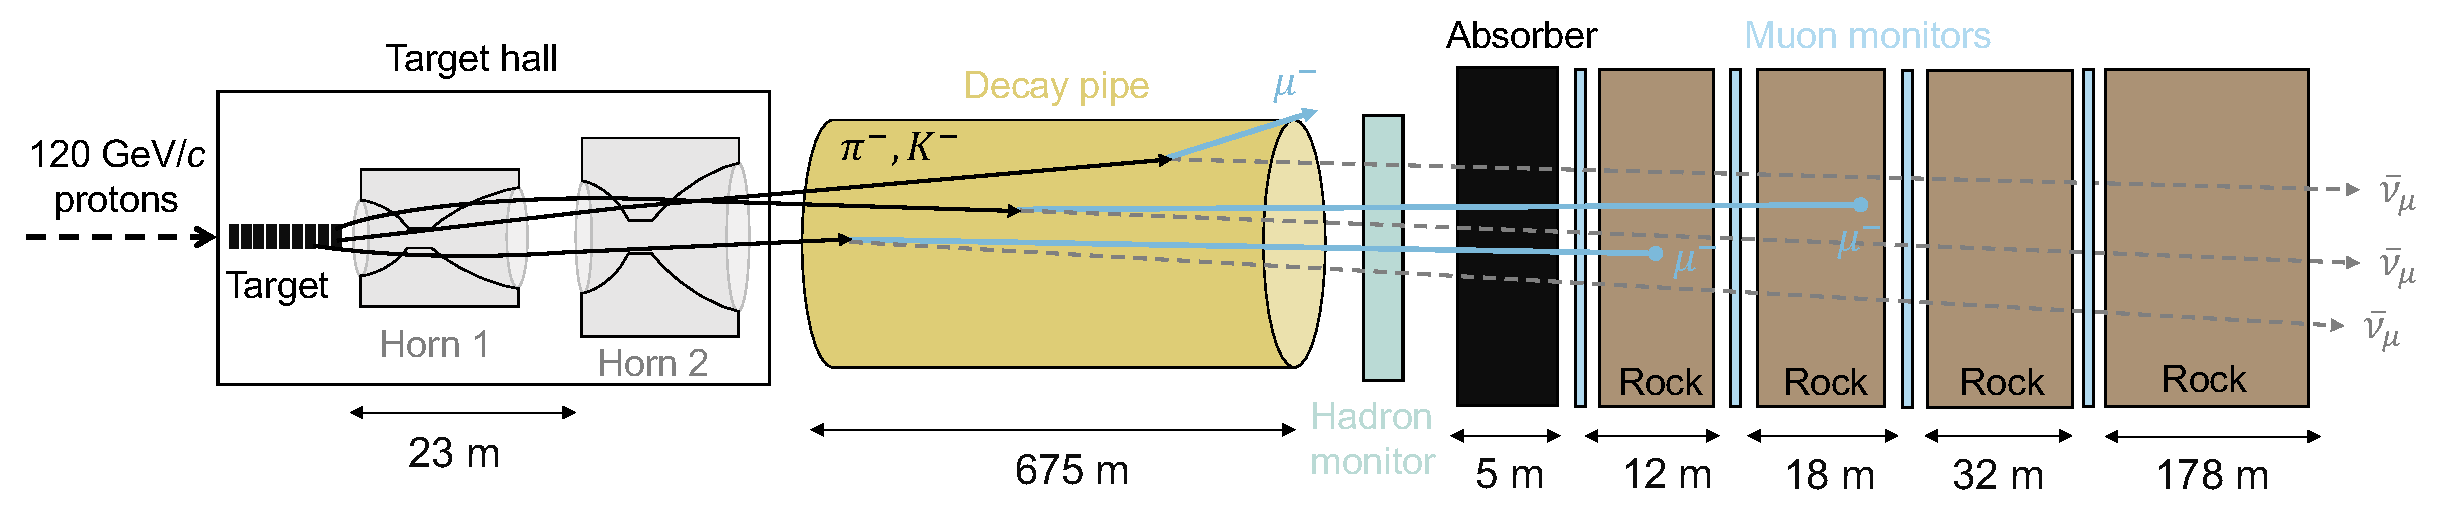
\includegraphics[width=1.\textwidth]{03minerva/figures/numiBeamline.pdf}}%
    \caption{Schematic illustrating the components of the NuMI beamline at Fermilab in the medium energy reverse horn current configuration, drawn based on the information provided in Refs.\cite{numi2016_ADAMSON2016279,TiceThesis2014}. }
    \label{fig:numi}
\end{figure}

\subsection{Instrumentation}

The NuMI beamline hardware and operations are in detail described in Ref.~\cite{numi2016_ADAMSON2016279}. First, protons from hydrogen ions undergo incremental acceleration in Fermilab's proton accelerator complex \cite{fnalAccelerator_Convery:2018ltx}, including the linear accelerator (Linac) and Booster synchrotron, ultimately reaching the final beam energy of 120~GeV in the Main Injector synchrotron accelerator.~Subsequently, these protons are extracted and directed onto the~graphite target in approximately 10~$\mu$s long windows, referred to as spills. Upon the extraction from the MI, the proton beam is also bent 3.343$^\circ$ (58.87~mrad) downwards towards the MINOS far detector in Minnesota.

Compared to the LE era, the beam intensity was increased from 400 kW to more than 700 kW in the ME era by placing more protons in the same spill and reducing the spill cycle time to 1.33~seconds from the original 2.2 seconds. The ME configuration delivered around 4.9$\times 10^{13}$ protons on target~(POT)\footnote{The number of protons on target (POT) is a metric used to characterise the integrated luminosity of the (anti)neutrino beam.} during each spill, resulting in the total data exposure of $1.12 \times 10^{21}$~POT recorded by MINERvA and used for this measurement.  The total number of POT collected by MINERvA over its physics run both in the LE and ME era is summarised in Table \ref{table:pot}.

\begin{table}[t!]
    \vspace{-10pt}
    \centering
    \begin{tabular}{c c c}
    \hline \\ [-1.5 ex]
    \multirow[c]{2}{*}{Regime}& \multicolumn{2}{c}{Mode (POT)} \\
    & Neutrino-dominated & Antineutrino-dominated\\ [0.5ex] % inserts table %heading
    \hline
    \hline \\[-1.8ex]
    Low (LE) $\sim$3~GeV & $4.0\times 10^{20}$ & $1.7 \times 10^{20}$ \\ 
    Medium (ME) $\sim$6~GeV & $10.6 \times 10^{20}$ & $11.2 \times 10^{20}$ \\
    \hline
    \end{tabular}

    \caption{The number of protons on target recorded by MINERvA in the low and medium energy regime for both neutrino and antineutrino-dominated beams.}
    \label{table:pot}
\end{table}


% To talk about the numi beam + angle
%https://lss.fnal.gov/archive/2015/pub/fermilab-pub-15-253-ad-fess-nd.pdf
% Upgrade to fermilab beam line for NOvA ,where I got the numbr  for the parameters
%https://ieeexplore.ieee.org/stamp/stamp.jsp?tp=&arnumber=4440873

Prior to reaching the graphite target, the proton beam is collimated by passing through a hole in the so-called baffle---a graphite-aluminum tube designed to partially degrade mis-steered beams to protect other components of the beamline. The proton beam size is about $\sim$1~mm upon impinging onto the 1.2~metres long (about 2.5 proton interaction lengths) graphite target. The target is made out of 50 narrow fins to dissipate heat and reduce the probability of reinteraction of produced hadrons, which are mounted on steel pipes providing water cooling and contained within a helium-filled vessel.

The final state particles produced by the proton beam hitting the target, mostly pions and kaons, are charge-sign selected and focused in a forward direction by two 3~metres long parabolic magnetic horns made of aluminum.~The choice of the horn current direction, whether it is forward horn current (FHC) or reverse horn current (RHC), determines the selection of positive or negative charged hadrons, ultimately resulting in a neutrino or antineutrino-dominated beam, respectively.~The RHC configuration is shown in Figure~\ref{fig:horns}. The horns increase the hadron flux in the desired energy range and provide flexibility in choosing that energy based on their configuration. The ME~spectra with the (anti)neutrino energy peak of $\sim$6~GeV was achieved by increasing the distance between the target and the first horn, and the first horn and the second horn compared to the LE configuration.\enlargethispage{2\baselineskip}~During the antineutrino-dominated runs used in this measurement, the magnetic field was generated by a~$-200$~kA electric horn current into the horns. 

\begin{figure}[t!] 
    \vspace{-10pt}
    \centering
    {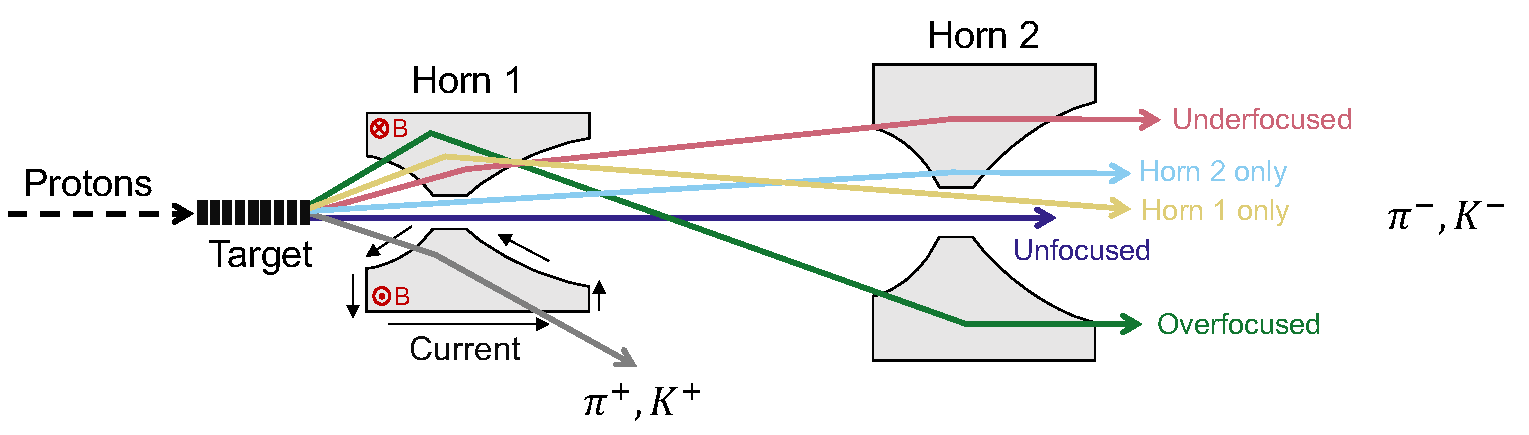
\includegraphics[width=1.\textwidth]{03minerva/figures/horns.pdf}}%
    \caption{Schematic of the working principle of the magnetic horns for the reverse horn current configuration indicating some possible trajectories, drawn based on the information provided in Ref.~\cite{AliagaSoplin:2016shs}. }
    \label{fig:horns}
\end{figure}

The first focusing horn perfectly focuses less than 10\% of charged hadrons producing antineutrinos, implying that the majority of hadrons require correction from the second focusing horn \cite{Bashyal:2021tzd}. Figure~\ref{fig:flux_focusComponents} illustrates the resulting antineutrino flux in both the ME configuration (used in this work's measurement) and the LE~configuration for comparison. Below 20~GeV, most antineutrinos are produced by pion decays, while antineutrinos produced from kaons dominate the high-energy tail. The bump observed at less than 1~GeV arises from low-energy antineutrinos produced by charged hadrons originating from outside the target. The rising part of the flux spectrum primarily originates from antineutrinos produced by charged pions that were initially overfocused by the first horn but subsequently corrected by the second horn. Conversely, the descending part of the flux corresponds to antineutrinos generated by underfocused charged pions, which are corrected by the second horn. 

\begin{figure}[t!] 
    \vspace{-5pt}
    \centering
    {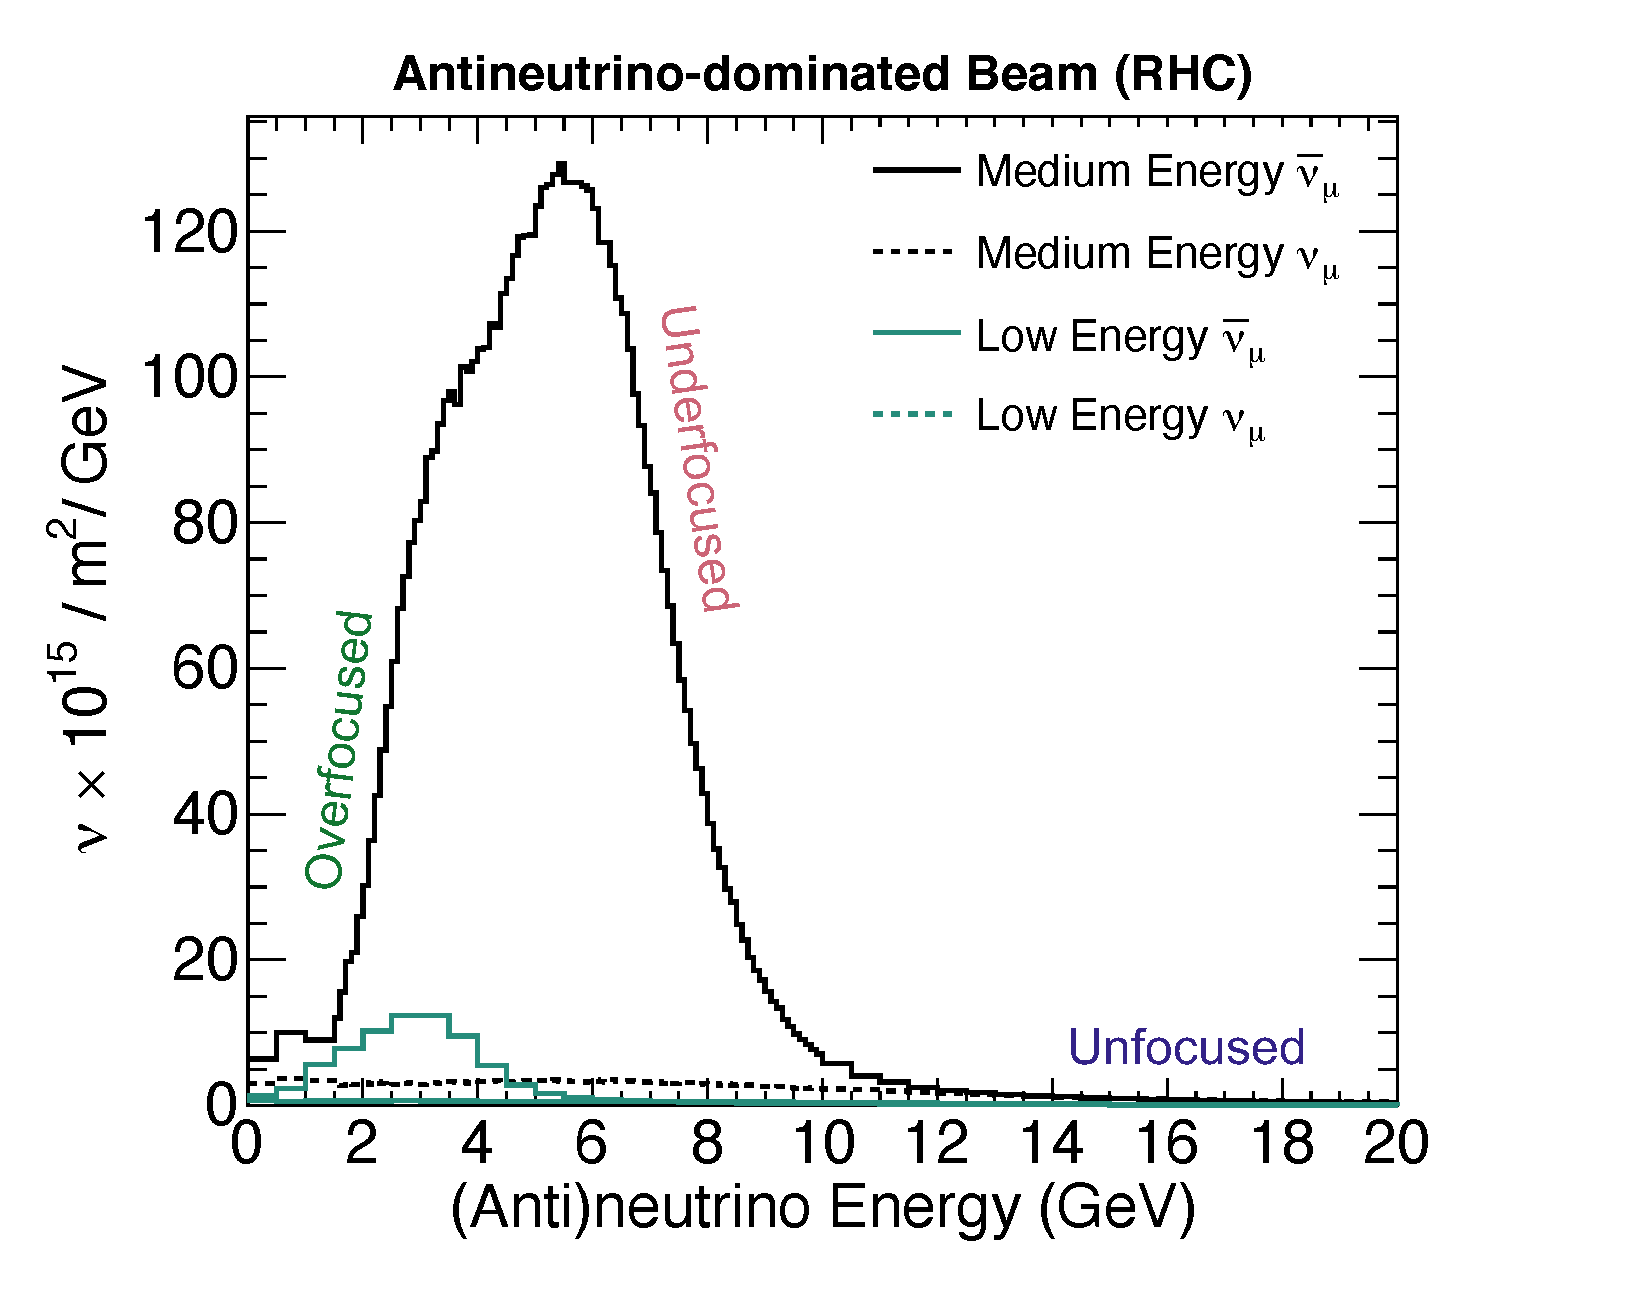
\includegraphics[width=.72\textwidth]{03minerva/figures/RHCflux_focusComponents.pdf}}%
    \caption{Distributions of (anti)neutrino fluxes in the medium and low energy regimes are depicted for the reverse horn current configuration at the MINERvA detector. These distributions represent the energy distributions of (anti)neutrino interactions per unit area. The solid lines represent the primary antineutrino contribution, while the dashed lines indicate neutrino contamination in the antineutrino-dominated beam. The contributions of specific antineutrino parent-focusing components are colour-coded to illustrate their trajectories in Figure~\ref{fig:horns}.}
    \label{fig:flux_focusComponents}
\end{figure}


Overall, the first horn predominantly focuses low-momentum charged pions, leading to the production of low-energy antineutrinos in comparison to the second horn. The inclusion of the second focusing horn significantly enhances the focusing, contributing to an increase of almost 50\% in the ME configuration \cite{Bashyal:2021tzd}. Some high-energy hadrons that are perfectly aligned with the magnetic horns can pass through without being charge-selected. Consequently, some of these hadrons decay into neutrinos, contributing to the contamination of the antineutrino-dominated beam, particularly at higher energies.

Focused negatively charged hadrons enter the 675~metres long decay pipe filled with helium to limit interactions with the hadron beam.~As they traverse the decay pipe, the hadrons primarily decay into muon antineutrinos via modes such as $\pi^{-}\rightarrow \mu^{-}\bar{\nu}_{\mu}$ with a~branching ratio exceeding 99\% and $K^{-}\rightarrow \mu^{-}\bar{\nu}_{\mu}$ with a branching ratio of 63.5\% \cite{numi2016_ADAMSON2016279,Workman:2022ynf}. The muon antineutrino beam is contaminated by $\nu_{\mu}$, $\nu_{e}$, and $\bar{\nu}_{e}$ due to other decay modes such as $K^{-}\rightarrow e^{-}\bar{\nu}_{e}\pi^{0}$ or $\pi^{-}\rightarrow \mu^{-}\bar{\nu}_{\mu} \rightarrow e^{-}\bar{\nu}_{e}\nu_{\mu}\bar{\nu}_{\mu}$ \cite{Workman:2022ynf}. Any remaining undecayed hadrons are detected by the hadron monitor and absorbed in the downstream\footnote{Downstream and upstream indicate positions relative to the beam direction, where downstream is in the direction of the beam, and upstream is against it.} hadron absorber made of aluminium, steel, and concrete. The only particles left in the beam---muons and antineutrinos---travel through 240~metres of dolomite rock interlaid  with four muon monitors as depicted in Figure~\ref{fig:numi}.\enlargethispage{2\baselineskip} 
The rock acts as a muon shield stopping the residual muons and allowing the antineutrinos to pass downstream to the MINOS near detector hall, which housed the MINERvA detector, located about 1~kilometre from the target. Some antineutrinos interact with the rock, creating additional antimuons referred to as rock muons, which could travel downstream to the MINERvA detector as well.
% rock muon - what they are
% Upgrade to fermilab beam line for NOvA ,where I got the number for the parameters
%https://ieeexplore.ieee.org/stamp/stamp.jsp?tp=&arnumber=4440873
% bunch is created around a particle which goes around the synchrotron with the frequency synced with the RF cavity
% beam description
% https://inspirehep.net/files/de0505656dd53c8c966da8531af0b55a
%hydrogen ions (H$^-$) are first accelerated to 400~MeV in the linear accelerator (Linac) and then converted into protons by passing through a carbon foil, which strips off the extra electrons going into the Booster, where they are subsequently further accelerated to 8~GeV. 

% https://lss.fnal.gov/archive/2015/pub/fermilab-pub-15-253-ad-fess-nd.pdf


\subsection{Simulation and characterisation}

% ME focusing uncertainties
% https://minerva-docdb.fnal.gov/cgi-bin/sso/ShowDocument?docid=16092
% ME hadron production uncertainties 
% page 228 - downloaded as eps and converted to pdf from 
% https://minerva-docdb.fnal.gov/cgi-bin/sso/ShowDocument?docid=12026

Precise knowledge of the (anti)neutrino flux produced by the NuMI beamline is crucial for (anti)neutrino cross-section measurements. In addition to determining the number of (anti)neutrinos that interacted in the detector, understanding how many were initially present in the beam is essential, as indicated in Equation~\ref{eq:xsec1D} in the following chapter. However, understanding the (anti)neutrino beam is challenging, primarily due to the complex processes involved in hadron production and the focusing components of the beamline. MINERvA addresses this challenge by employing a calculated \textit{a priori} flux, i.e. simulated flux adjusted using external hadron production data with varying parameters related to both hadron production and focusing to incorporate relevant systematic uncertainties. Direct flux measurements are also possible \cite{Loiacono2010} but are limited to an accuracy of 15\% due to poorly constrained backgrounds and detector uncertainties. 


The NuMI beam is simulated using the G4NuMI package, which is based on the GEANT4 (GEometry ANd Tracking) software version 9.4.p02~\cite{Geant4_AGOSTINELLI2003250,Geant4_1610988}, incorporating detailed geometrical models of the beamline.~The G4NuMI package, initially developed for MINOS \cite{Pavlovic2008, Koskinen2009, Loiacono2010}, was subsequently improved by MINERvA \cite{AliagaSoplin:2016shs, PhysRevD.94.092005}. It covers the entire process from the 120 GeV/$c$ protons impinging onto the graphite target to focused charged hadrons decaying into (anti)neutrinos, predicting the number, flavour, and momentum distributions. The underlying phenomenological hadronic models FRITIOF precompound \cite{Andersson:1986gw, Nilsson-Almqvist:1986ast} and Bertini cascade \cite{Bertini1963_PhysRev.131.1801,Guthrie:1968ue, Bertini1969_PhysRev.188.1711,BERTINI1971670} implemented in the FTFP\_BERT package of GEANT4 to predict the hadrons produced by the proton-carbon interactions were, however, shown to disagree with external hadron production data \cite{AliagaSoplin:2016shs}.
Therefore, MINERvA developed the Package to Predict the Flux (PPFX) \cite{AliagaSoplin:2016shs,Aliaga_2014} to constrain these models using external experimental data. 


%The PPFX primarily uses the NA49 \cite{Alt_2007} and the MIPP \cite{PhysRevD.90.032001} pion production datasets, which are corrected to the NuMI appropriate energy scale using the FLUKA simulation \cite{Ferrari:2005zk, BOHLEN2014211}. The NA49 experiment at CERN measured the pion production on a thin, i.e.~a~few percent of interaction length, carbon target using a 158~GeV/$c$ proton beam \cite{Alt_2007}. The MIPP experiment measured pion production on a replica of the LE NuMI target (about 2~proton interaction lengths) using a 120 GeV/$c$ protons \cite{PhysRevD.90.032001}. Additional datasets are also employed in the PPFX to constrain kaon and nucleon production, as well as the absorption of particles in beamline materials as described in detail in Ref.~\cite{PhysRevD.94.092005}.

% MIPP not used because thick target constraint doesn't agree with low nu method

The PPFX primarily uses the NA49 \cite{Alt_2007} pion production dataset, which is corrected to the NuMI appropriate energy scale using the FLUKA simulation \cite{Ferrari:2005zk, BOHLEN2014211}. The NA49 experiment at CERN measured the pion production on a thin, i.e.~a~few percent of interaction length, carbon target using a 158~GeV/$c$ proton beam \cite{Alt_2007}. \enlargethispage{1\baselineskip}Additional datasets are also employed in the PPFX to constrain kaon and nucleon production, as well as the absorption of particles in beamline materials as described in detail in Ref.~\cite{PhysRevD.94.092005}. Uncertainties from each of these datasets are incorporated in the hadron production correction reweight of the base simulation. For interactions with no available data, the uncertainty is evaluated using the spread of various hadronic models in GEANT4. 

\begin{figure}[t!] 
    \vspace{-20pt}
    \centering
    {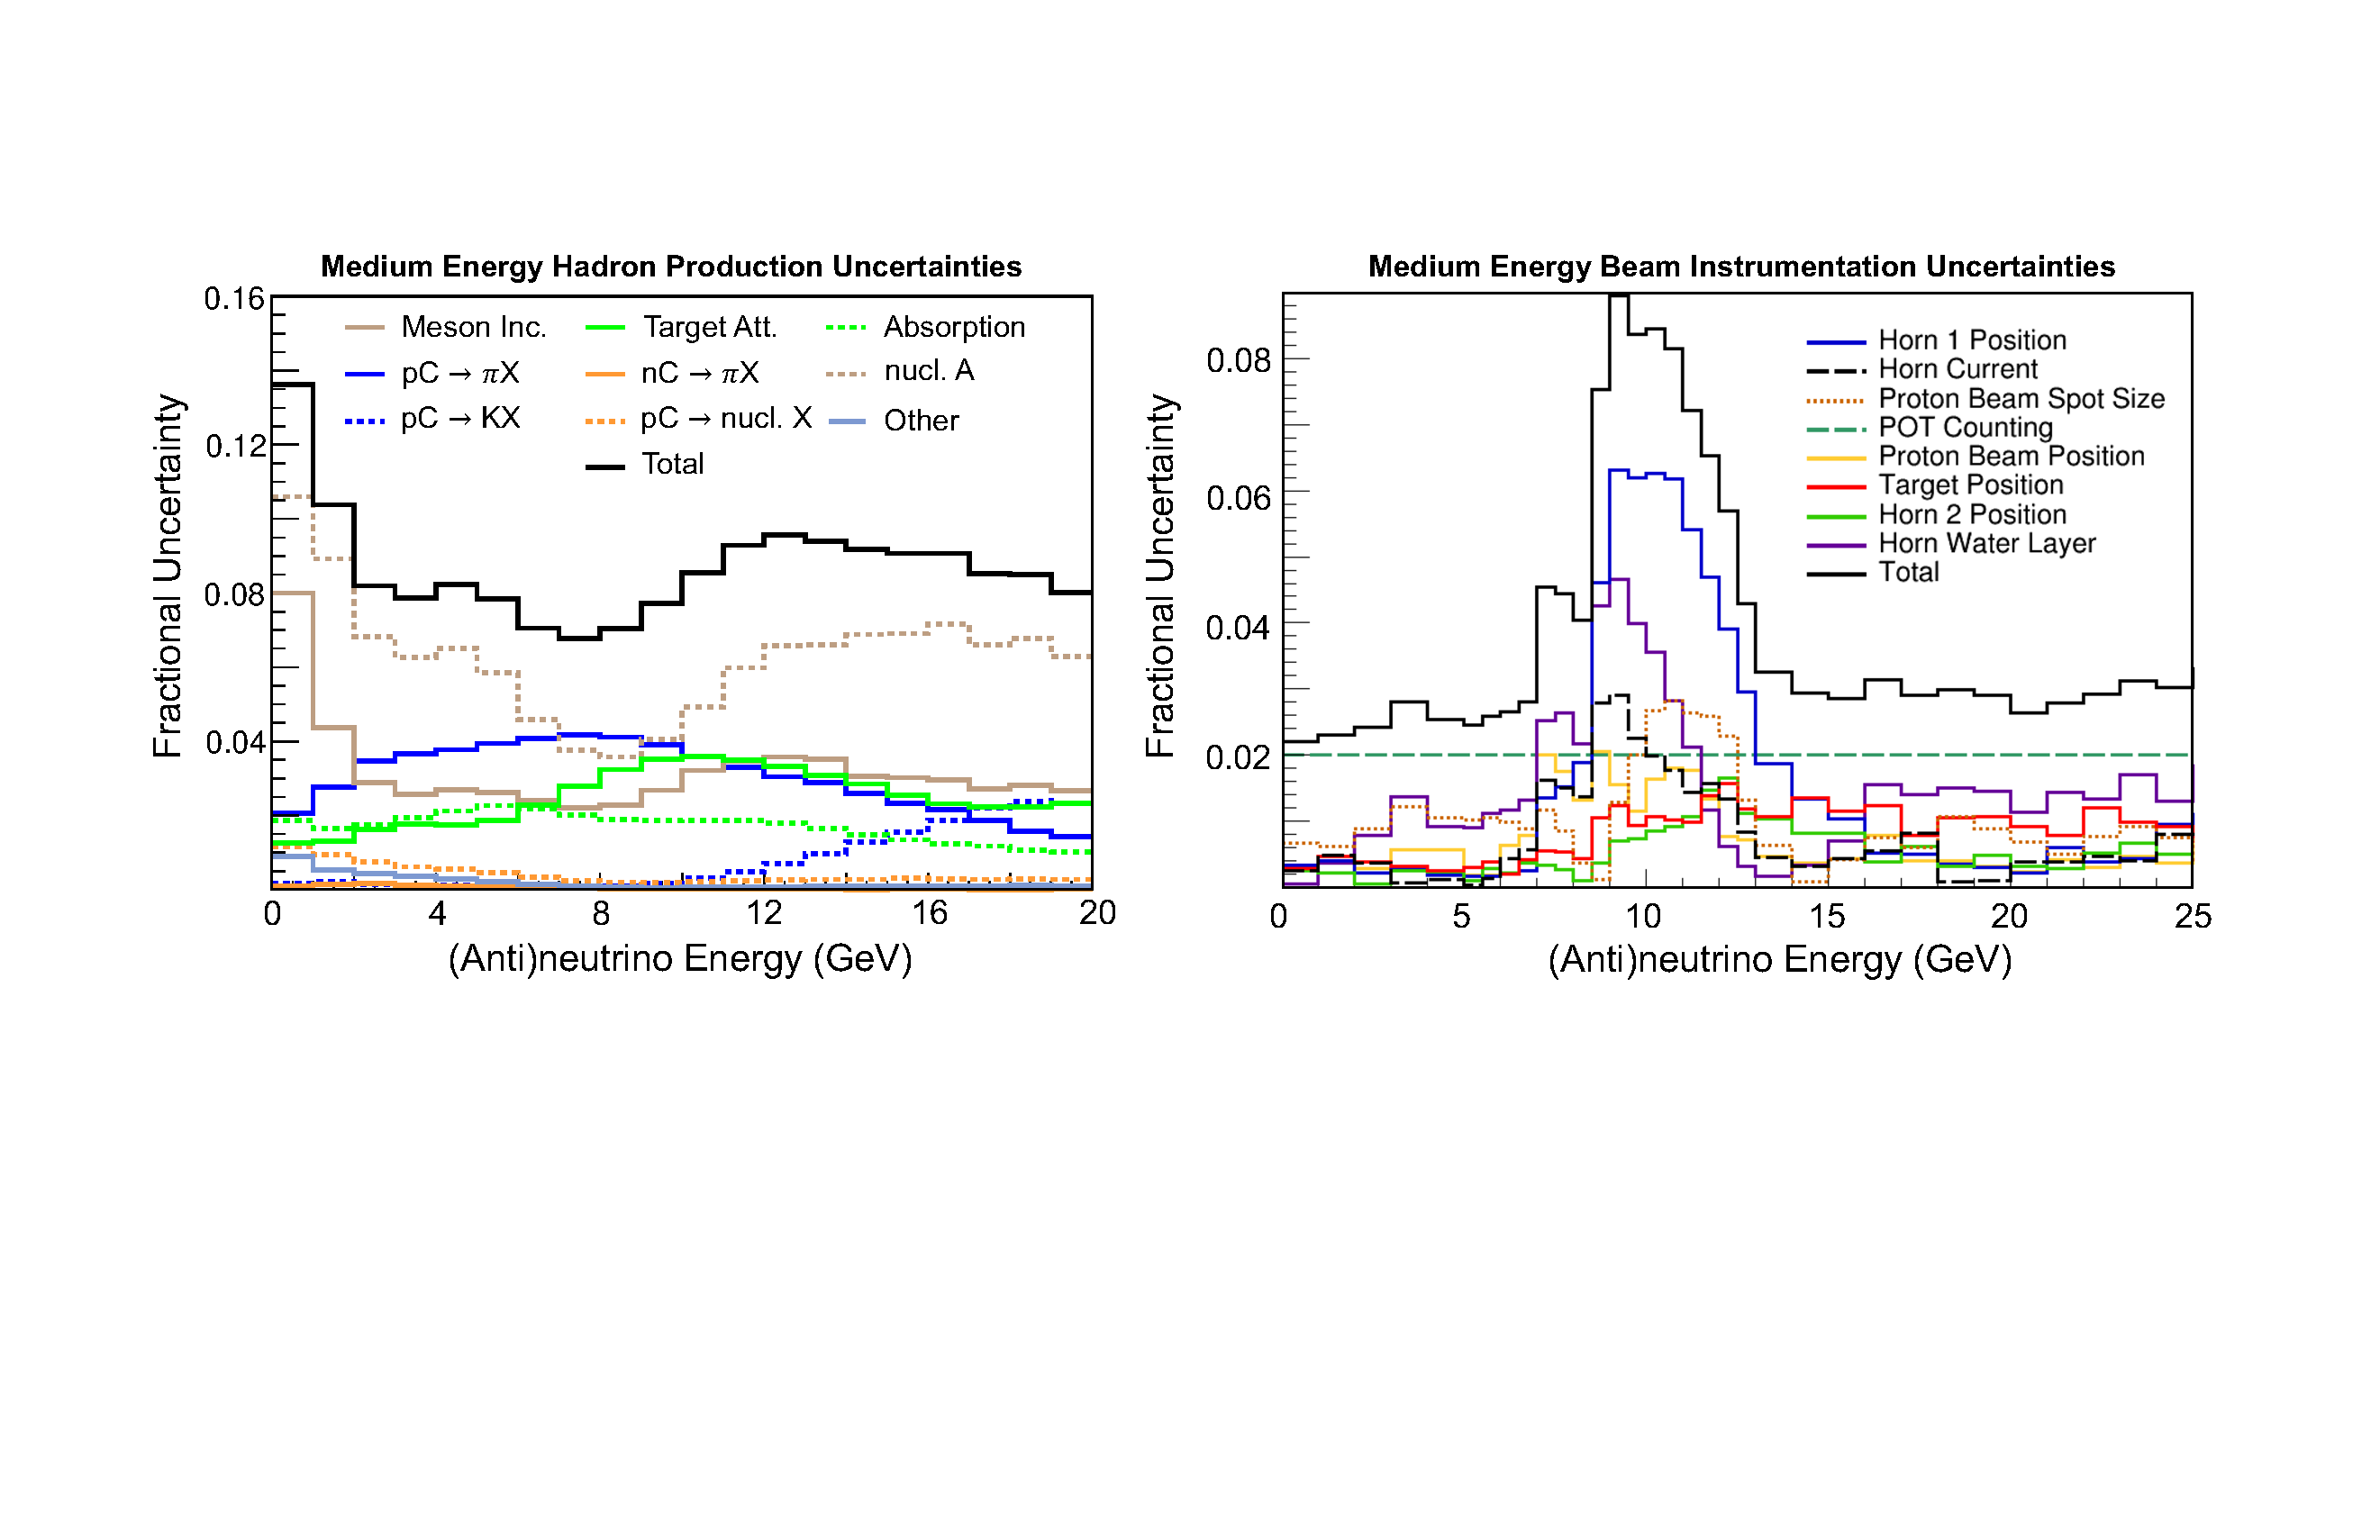
\includegraphics[width=1\textwidth]{03minerva/figures/ppfx_unc.pdf}}%
    \caption{PPFX uncertainties on the NuMI medium energy flux. Left: Flux uncertainty from different hadron interaction categories modified from Ref.~\cite{AliagaSoplin:2016shs}. Note that `Meson Inc.' refers to the uncertainty of mesons interacting on any material in the beamline, `Target Att.' and `Absorption' are the uncertainties due to the absorption of particles in the target and other materials, respectively, `nucl. A' represents mainly nucleons interacting in material that is not carbon, and `Other' includes any other interactions. Right: Beam geometry and focusing uncertainties modified from Ref~\cite{Messerly:2019itw}. `Baffle Scraping' represents the uncertainty on the tails of the proton beam interacting with the baffle.}
    \label{fig:ppfx_unc}
\end{figure}

The hadron production uncertainties are then propagated to the (anti)neutrino energy distribution using a so-called multiverse method \cite{MAT_Messerly_2021}.~A collection of 100 flux predictions, referred to as universes, is created by randomly sampling from a multidimensional Gaussian distribution centred on the default parameter values of hadron production cross-sections varied within their uncertainties and taking into account correlations between the parameters. The spread of the universes in each bin provides the \textit{a priori} flux uncertainties arising from the hadron production, as depicted in Figure~\ref{fig:ppfx_unc} for the NuMI beam in medium energy.

Furthermore, PPFX also enables the implementation of uncertainties arising from beamline instrumentation, such as the position of the target relative to the horn, the current applied to the magnetic horns, or the residual water layer on horns due to cooling. \enlargethispage{1\baselineskip}These uncertainties can be evaluated similarly to the hadron production uncertainties and are also depicted in Figure~\ref{fig:ppfx_unc} for the NuMI beam in medium energy. Overall, the flux uncertainty is dominated by hadron production, except in the falling edge of the (anti)neutrino distribution, where focusing uncertainties dominate. Additionally, MINERvA also improves the flux through \textit{in-situ} measurements of processes with known cross-sections, as discussed in Chapter~\ref{ch:dataAsimulation}.


\section{MINERvA detector}\label{sec:MINERvAdetector} 

\begin{figure}[b!] 
    \centering
    {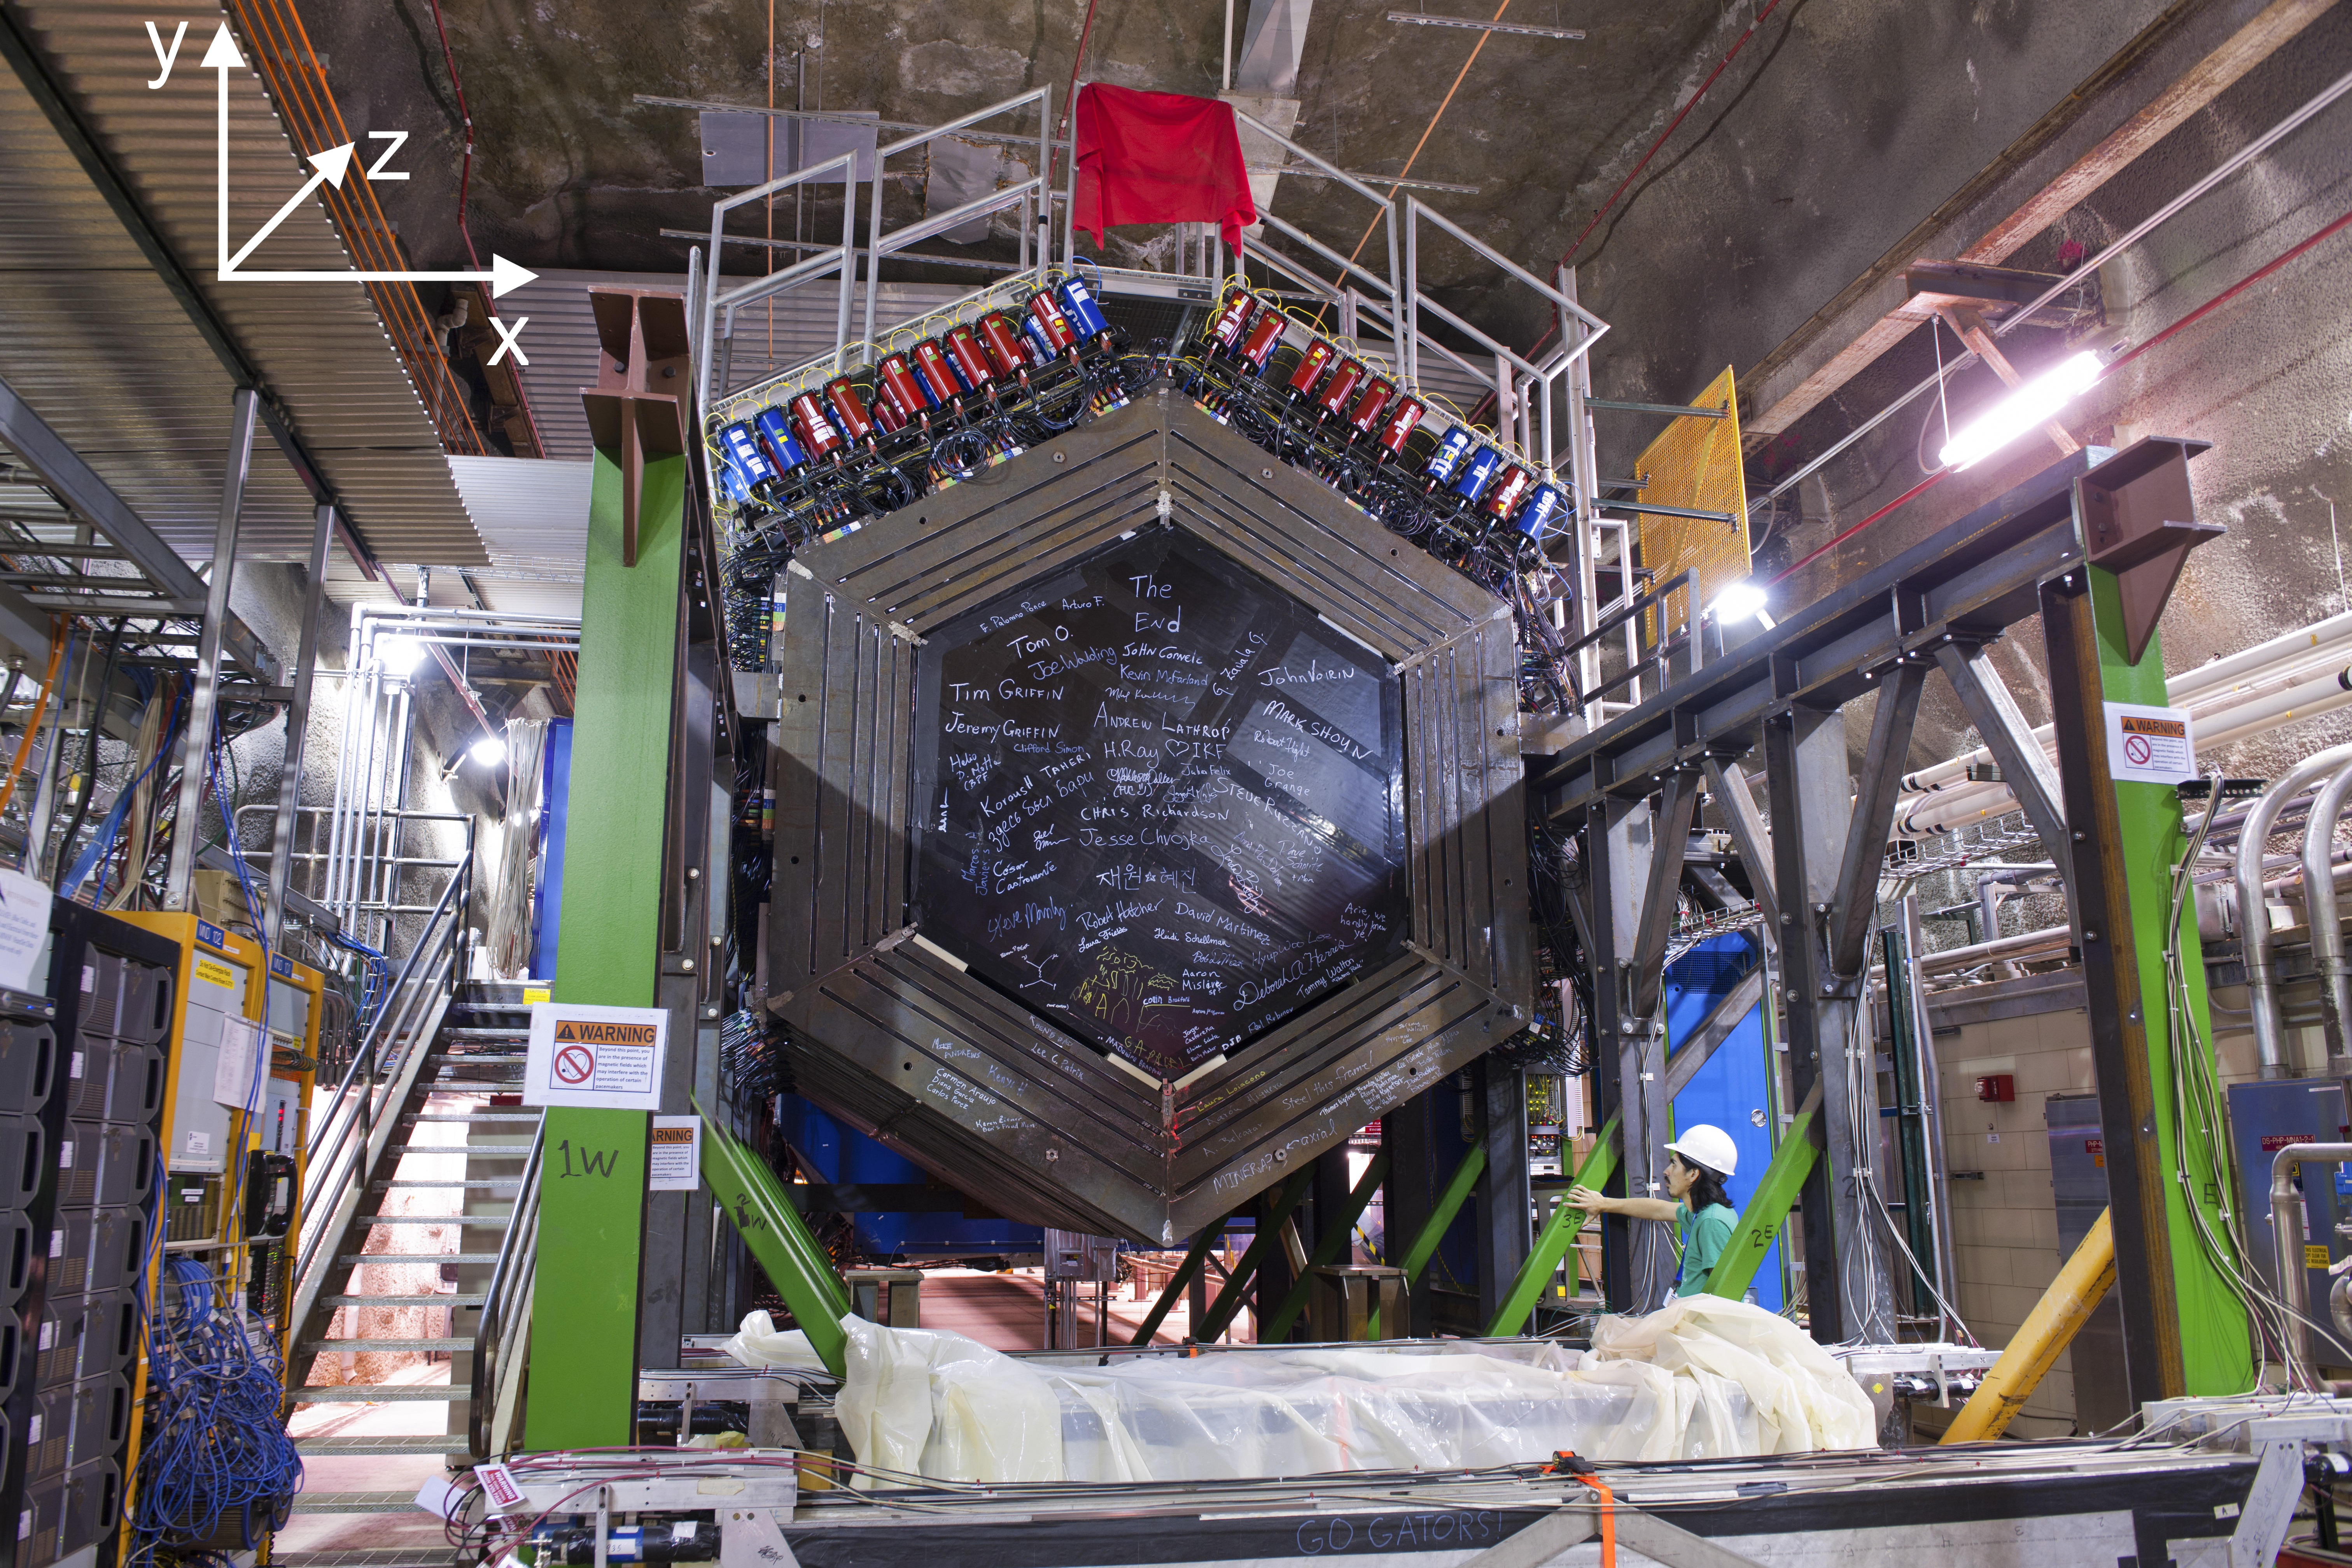
\includegraphics[width=0.9\textwidth]{03minerva/figures/minerva_photo.jpg}}%
    \caption{Photo of the front view of the MINERvA detector showing the last installed module. The signed black plane is the inner detector, while the metal frame around is the outer detector. The red and blue cylinders on the top of the detector depict the optical readout system. Permission to reuse granted by Fermilab Creative Services. Credit: Reidar Hahn, Fermilab.}
    \label{fig:detectorPhoto}
\end{figure}


The MINERvA detector~\cite{Aliaga_2014} was located approximately 100~metres underground in the MINOS near detector hall and about 1~kilometre away from the graphite target of the NuMI beamline. As shown in Figure~\ref{fig:detectorPhoto}, MINERvA itself was a hexagonal detector made of an inner detector part in black that is mounted within a metal outer detector frame. On the top of the frame, there was an optical readout system in red and blue. \enlargethispage{1.5\baselineskip}The detector design and methods of operations were fundamental in enabling MINERvA to identify and study (anti)neutrino interactions.

Akin to other particle detectors, MINERvA worked like a very fast camera, capturing `snapshots' in both space and time of the energy deposited in the detector by particles resulting from interactions between (anti)neutrinos and the detector material. An example of such a `snapshot', referred to as an event, is shown in Figure~\ref{fig:eventDisplayDIS}. MINERvA's detection capability depended on two key elements: first, the use of finely segmented solid plastic scintillator technology for the active regions, enabling the measurement of energy deposits; and second, fast timing resolution ($\sim$5 ns) to distinguish overlapping events within a single spill, determining how quickly and frequently MINERvA could capture these `snapshots'.


\begin{figure}[t!] 
    \vspace{-15pt}
    \centering
    {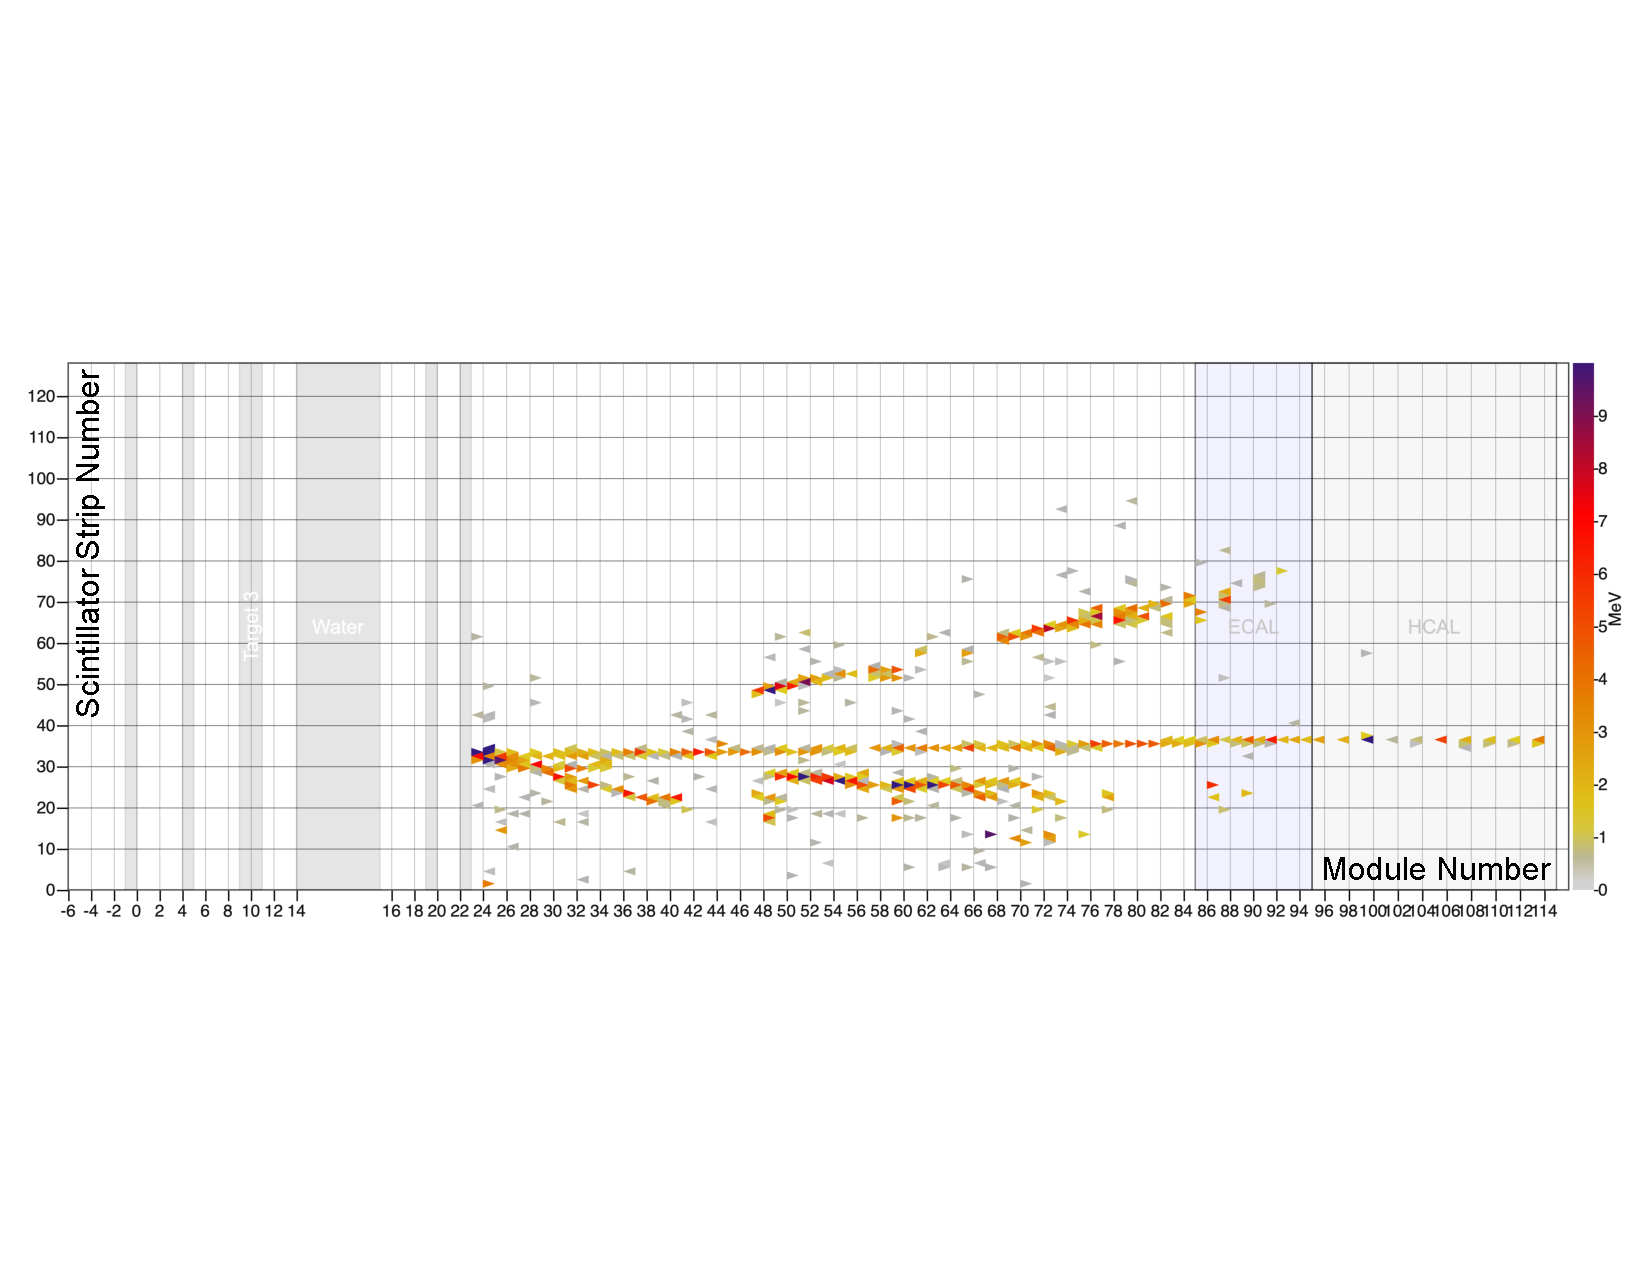
\includegraphics[width=1\textwidth]{03minerva/figures/dis_eventDisplay_new.pdf}}%
    \caption{Simulated antineutrino deep inelastic scattering (DIS) interaction in the MINERvA detector. The antineutrino interacts with a lead nucleus in target 5, producing an antimuon (the longest track) and multiple hadrons showers. The individual triangles are the energy deposits with their colour representing the size of the deposit.~The $x$-axis depicts the detector module number along the general direction of the beam. }
    \label{fig:eventDisplayDIS}
    \vspace{-2pt}
    %$\mu^{+}$ 3 protons, 2 $\pi^{0}$ and neutron
\end{figure}

MINERvA used a right-handed coordinate system with an origin at the centre of the detector, which is superimposed on the front view of the detector in Figure~\ref{fig:detectorPhoto}. In this system, the $z$-axis pointed downstream along the central axis of the detector, $y$-axis was pointed upwards, and the $x$-axis was directed to the left from the perspective of the beam. The (anti)neutrino beam itself, therefore, pointed 3.34$^{\circ}$ downwards in the $y$-$z$~plane. 

Figure~\ref{fig:detectorView} shows a schematic of the complete side view of the detector. As depicted, the upstream part of the inner detector consisted of the nuclear target region including carbon, iron, lead and water interleaved between the plastic scintillator planes, enabling the study of nuclear effects in (anti)neutrino interactions.\enlargethispage{2\baselineskip}~The main fiducial volume comprised the central tracking region, composed purely of finely segmented plastic scintillator planes to resolve and identify multi-particle final states, as well as track low-energy particles with energies greater than about 100~MeV. 

\begin{figure}[t!] 
    \vspace{-8pt}
    \centering
    {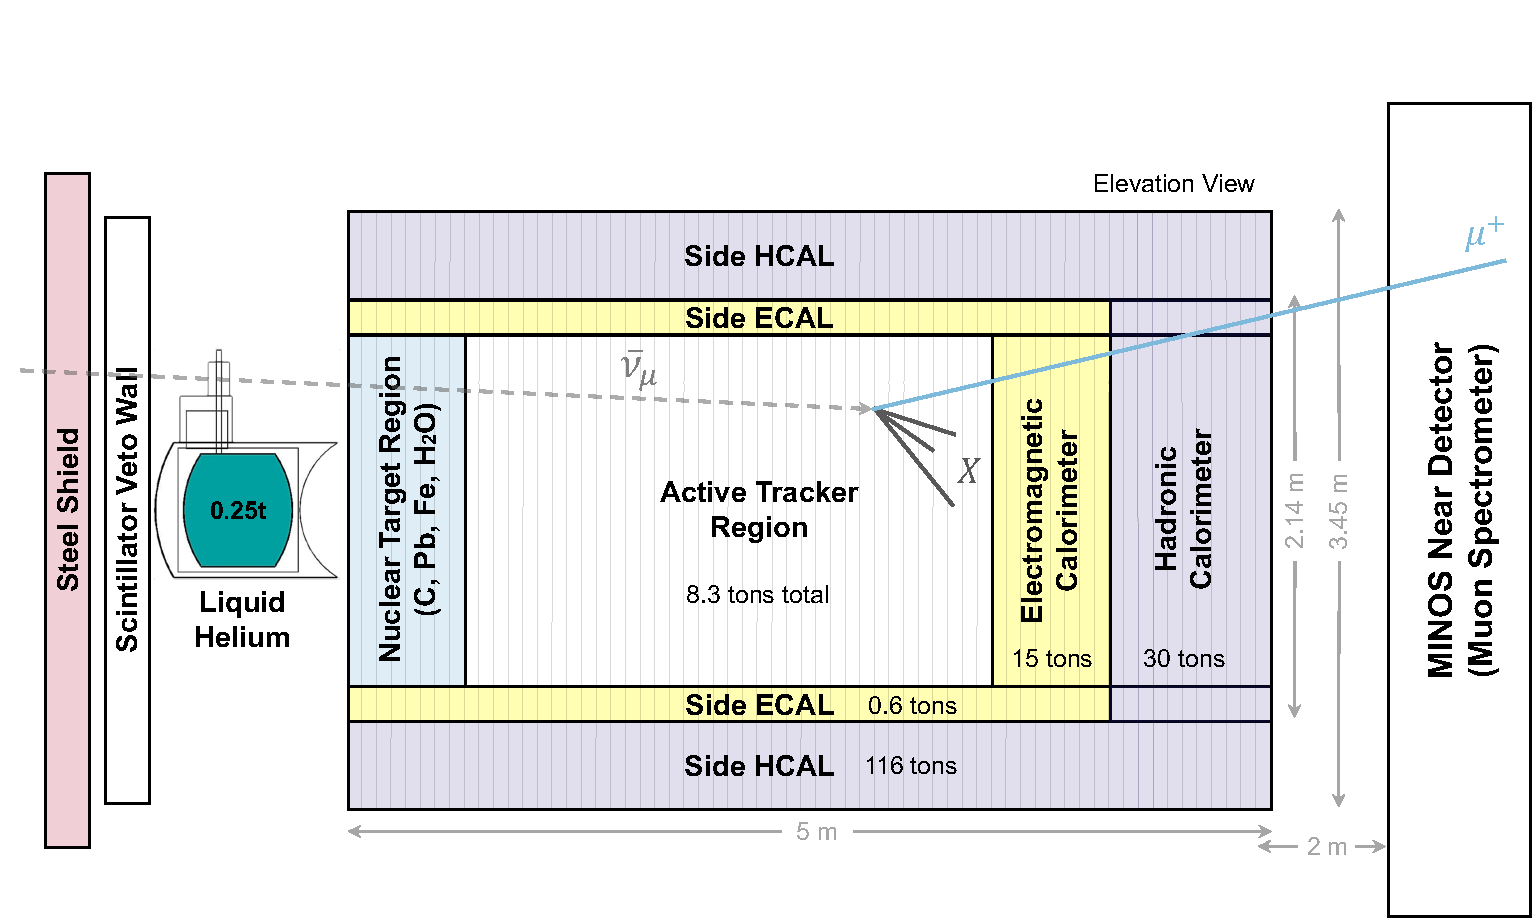
\includegraphics[width=1\textwidth]{03minerva/figures/minerva_view.pdf}}%
    \caption{Schematic side view of the MINERvA detector. Modified from Ref.~\cite{Aliaga_2014}.}
    \label{fig:detectorView}
\end{figure}

To contain electromagnetic showers and high-energy hadronic final states in the direction of the beam, the tracker was followed by alternating layers of lead--scintillator and steel--scintillator in the sampling electromagnetic (ECAL) and hadronic calorimeter (HCAL), respectively. Additionally, the outermost 15~cm of each ID plane was covered by steel side ECAL to reduce the amount of energy leaving the ID in the $x$-$y$~plane. For full containment and also acting as a support structure, the ID was surrounded by the outer detector (OD) lead hadronic calorimeter with four embedded scintillator strips visible in Figure~\ref{fig:detectorPhoto}.

MINERvA was able to tag the highly-energetic rock muons before they entered the detector and reject low-energy hadrons produced in the rock using a veto wall upstream of the main detector, consisting of a steel shield and scintillator. Between the veto wall and the front face of the main body of the detector, there was a liquid helium target in an aluminium cryostat, offering opportunities to measure (anti)neutrino interactions with somewhat less complicated and more easily predicted nuclear effects than heavier targets. The MINOS near detector, located downstream of the main MINERvA detector, functioned as a spectrometer for (anti)muons that were not contained within the MINERvA detector. This is further discussed in Section~\ref{sec:MINOS}.

% add plane numbers
% 20 ECAL
% 10 HCAL

\subsection{Scintillator planes}

Each hexagonal plane of the ID was made of 127 triangular solid scintillator strips of variable lengths of $\mathcal{O}$(1~m) stacked in the $x$-$y$~coordinate plane. Depending on the arrangement of the strips, there were three possible plane orientations, $X$, $U$, and $V$, referred to as views, which are illustrated in Figure~\ref{fig:scintillator}. The $X$-view consisted of scintillator strips running in parallel to the $y$-axis, whereas $U$- and $V$-view had strip arrangement rotated 60$^{\circ}$ clockwise and anticlockwise from the $X$-view, respectively. Figure~\ref{fig:scintillator} also shows the stacking of different views in the detector, where each $X$-view is alternately followed by either a $U$- or $V$-view. A so-called tracking module is formed by two planes, either $XU$ or $XV$. Although typically only two orthogonal planes (along with the time dimension) are required for three-dimensional reconstruction, the three different views provided an opportunity to mitigate potential ambiguities in reconstructed hit associations seen when multiple tracks traverse two orthogonal planes. 


\begin{figure}[b!] 
    \vspace{-5pt}
    \centering
    {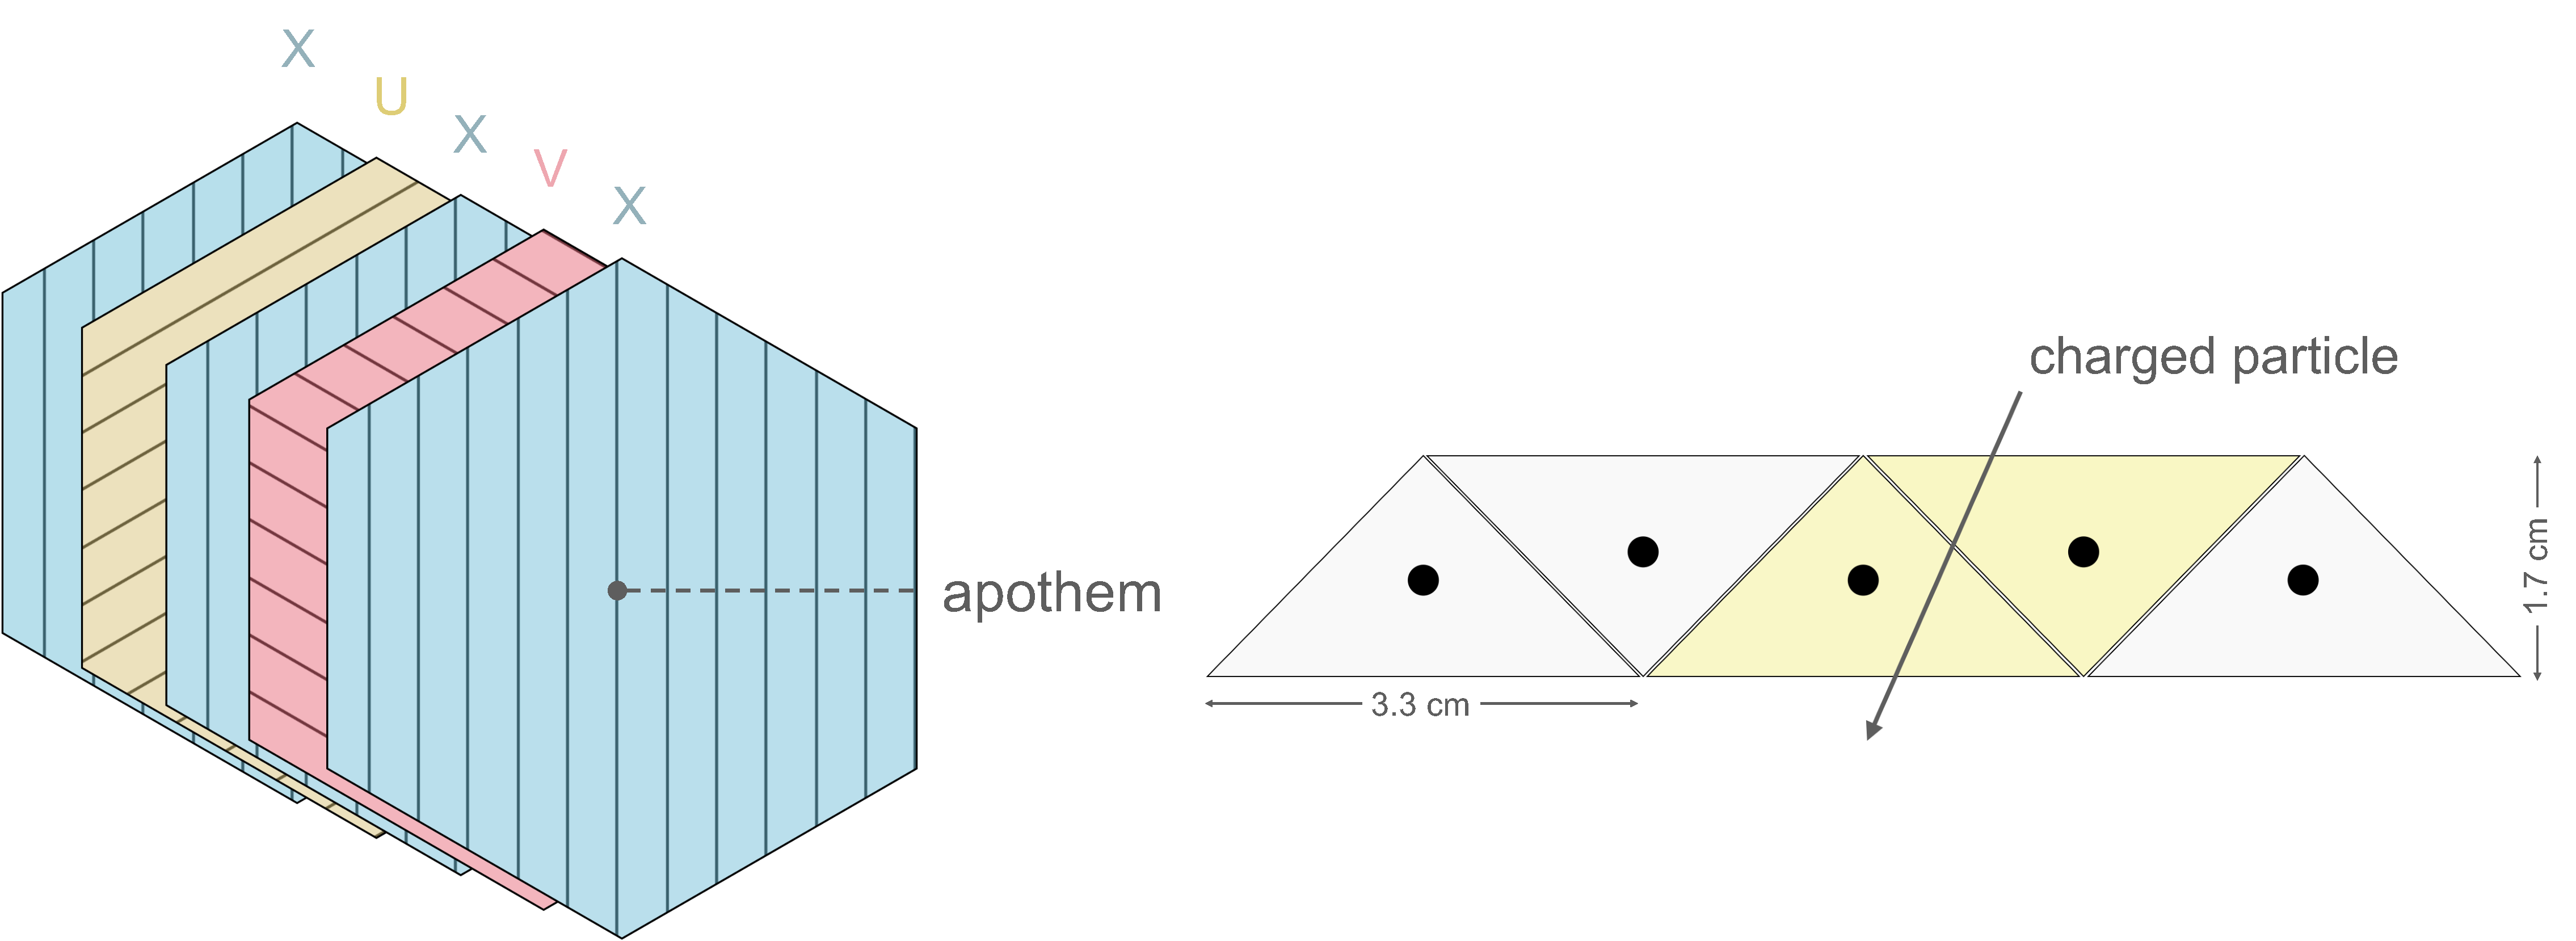
\includegraphics[width=1\textwidth]{03minerva/figures/scintillator.pdf}}%
    \caption{Left: Diagram of the three views of scintillator planes and their stacking in the detector. Right: Cross-section of the configuration of triangular scintillator strips, i.e. bars, making up one scintillator plane, showing the impact of a charged particle passing through.}
    \label{fig:scintillator}
\end{figure}


The individual scintillator strips, primarily made of doped polystyrene, i.e. hydrocarbon (CH), were glued and sealed together light-tight with epoxy to prevent light leaks. Additionally, polycarbonate sheets were applied to enhance the overall rigidity of the assembly. Each scintillator strip was also coated by reflective titanium dioxide for optical isolation. \enlargethispage{1\baselineskip}Figure~\ref{fig:scintillator} demonstrates that the triangular strips were overlaid in such a way that a charged particle passing through a plane would deposit energy and hence create a scintillation signal, i.e.~blue light, in at least two scintillator strips. The scintillation light was collected via wavelength shifting (WLS) fibres at the centre of each strip further discussed in Section~\ref{sec:opticalReadout}. 

Note that in contrast to the ID, the scintillator strips embedded in the OD were rectangular with bigger cross-sections.

\subsection{Nuclear target region}

MINERvA's unique capability to perform self-contained measurements of nuclear dependence in (anti)neutrino scattering stems from the nuclear target region. It was composed of five solid passive, i.e. not instrumented, targets made of transverse segments of carbon~(C), iron~(Fe), and lead~(Pb), interlaid with tracking modules (made of two scintillator planes each) as depicted in Figure~\ref{fig:targetRegion}. While the geometry of the individual targets may seem complex, it, for example, allowed for the investigation of acceptance differences at various regions of the detector due to the MINOS near detector acceptance constraint discussed later on in Section~\ref{sec:MINOS}. Furthermore, the patterns were chosen so that (anti)neutrinos that did not interact within the nuclear target region would traverse approximately the same amount of material throughout the target region, irrespective of their trajectory in the $y$-$z$~plane. 

\begin{figure}[t!] 
    \vspace{-5pt}
    \centering
    {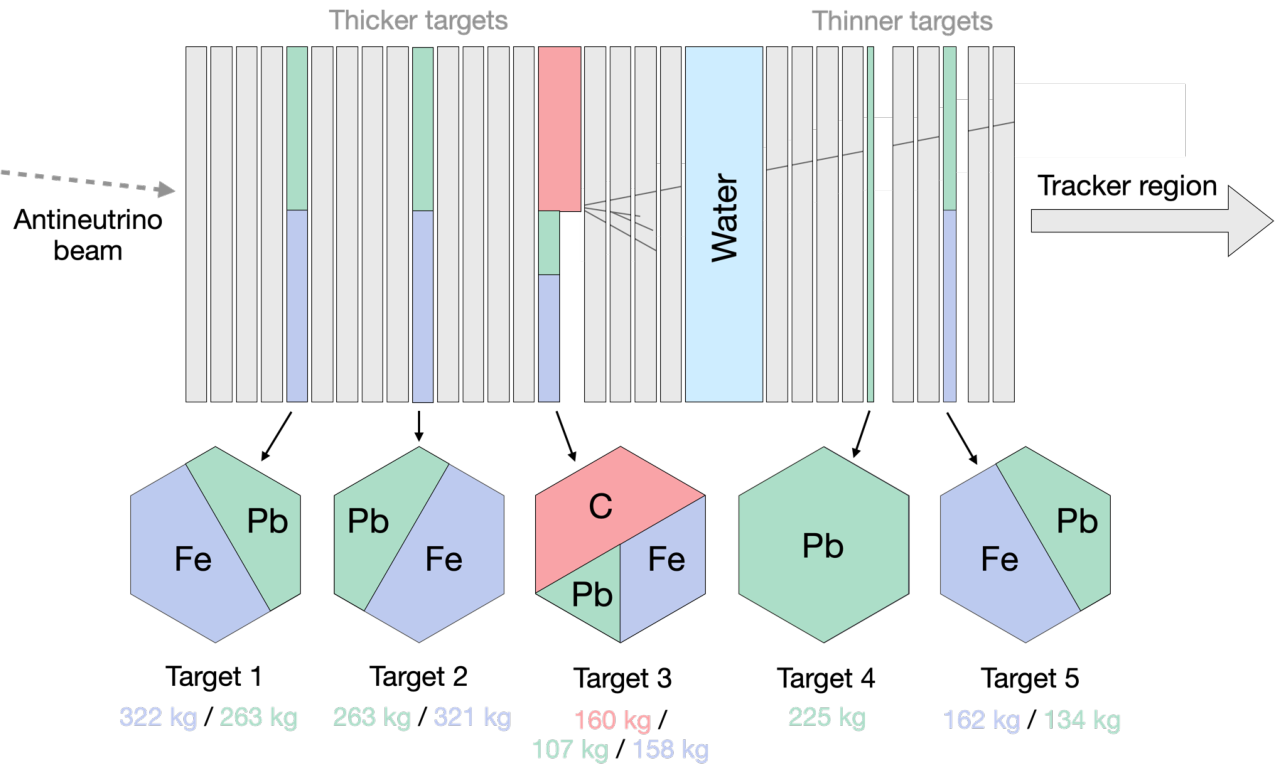
\includegraphics[width=1\textwidth]{03minerva/figures/targetRegion.pdf}}%
    \vspace{10pt}
    \caption{Diagram of the nuclear target region in the MINERvA detector. The individual target cross-sections are depicted looking downstream of the detector. The fiducial mass information was taken from Ref.~\cite{Aliaga_2014}.}
    \label{fig:targetRegion}
\end{figure}

Figure~\ref{fig:targetRegion} also shows the geometrical division of the individual target planes into different materials as visible when looking downstream of the detector. Both targets 1 and~2 were composed of roughly 60\% iron and 40\% lead in terms of fiducial area, with a plane thickness of about 2.6~cm (about one tracking module). However, they contained nearly the same amount of fiducial mass of iron and lead. The orientation of iron and lead in target 2 was flipped horizontally, i.e.~reflected around the $y$-axis, with respect to target 1. As the most upstream target, target 1 was affected by a limited number of upstream tracking planes used to identify particles produced outside the MINERvA detector, particularly the rock muons. This aspect is relevant in the context of this work's measurement discussed later in Section~\ref{sec:eventSelection}.

Target 3 consisted of 50\% carbon, approximately 33\% iron and 17\% lead, i.e. 1/3 iron and 1/6 lead, respectively, allowing for detailed studies of nuclear dependence in (anti)neutrino scattering within one target. The carbon provided valuable cross-validation for the (anti)neutrino interaction cross-sections in plastic scintillator (hydrocarbon) and vice versa, as they are expected to be approximately the same. In general, (hydro)carbon data was crucial for comparison with results from other experiments such as T2K~\cite{t2k_ABE2011106}. Target 3 was the thickest of all the solid targets to ensure sufficient fiducial mass for the light carbon. The iron and lead parts had the same thickness as in targets 1 and 2, while the carbon component was about 7.6~cm thick. All materials were aligned at the upstream end, resulting in an air gap downstream of the iron and lead components. 

Target 4, the thinnest in the series (comprising less than 1/3 of a tracker module), was constructed using pure lead to ensure the conversion of any produced photons from either upstream or downstream targets. The chosen thickness, approximately 1.5 radiation lengths, allowed photons to initiate a shower but not enough to be fully contained. This strategy improved event containment in the upstream targets and concurrently reduced noise from photons (or $\pi^0$s and neutrons), minimising potential confusion in tracker reconstruction and event selection. Its reduced thickness resulted in an air gap between the target and the first downstream scintillator plane. 

Target 5, located directly upstream of the fully active tracking region, had the same shape as target 1 but only half of its thickness (about half of a tracker module). It was designed for the study of lower-energy particles and particle multiplicities, benefiting from enhanced tracking and energy resolution. Similar to targets 3 and 4, there was an air gap between target 5 and the following tracker module, which also allowed for better spatial separation of low-energy final state particles. 

Placing thicker targets upstream was done to minimise interference with particles resulting from interactions in downstream targets, thereby optimising the reconstruction of (anti)neutrino interactions and their exclusive final states.

In addition, there was a water target located between the solid targets 3 and 4. It consisted of a circular neoprene balloon filled with (liquid) water suspended on a circular steel frame and held in place with sheets made of polyamide synthetic fibre. The water target thickness varied between 17~cm at the edge of the balloon to 24~cm at the centre of the balloon, with the water volume measured when the target was emptied. The water target is not included in this work's measurement, similar to the helium target described earlier.

In general, each target was separated by four tracking modules, except target 4 and target 5, which were separated by only two tracking modules. \enlargethispage{1\baselineskip} Figure~\ref{fig:targetRegion} demonstrates how the active layers between the targets enabled the identification of the location of (anti)neutrino interactions and tracking of final state particles. 

\subsection{Optical readout and data acquisition}\label{sec:opticalReadout}

A wavelength-shifting (WLS) fibre embedded in the centre of each scintillator strip absorbed the produced blue scintillation light, re-emitting it inside the fibre as green. The WLS fibres then directed the light out of the detector, connecting to clear optical fibres. The shifted green light was reflected internally within the fibre as it travelled, minimising the signal reduction, while the end of the fibre not pointed towards the readout system was mirrored to reflect the light back.

The clear optical fibres from adjacent scintillator strips were grouped in sets of eight. Eight sets of these optical fibre groups were connected to one photomultiplier tube (PMT) with 64 channels, i.e., an 8×8 array of pixels, which converted the collected light into charge. The fibres were interleaved in such a way that the light signal from adjacent scintillator strips did not go into adjacent pixels of the PMT to prevent signal cross-talk. The PMT converted collected photons into photoelectrons via the photoelectric effect on its photocathode, wherein light incident on a metal surface with energy above the material's binding energy ejected electrons. Subsequently, the electrons were multiplied going through a chain of dynodes with high potential differences between succeeding dynodes. Electrons collided with each anode, producing more electrons, which eventually reached the anode end of the tube, resulting in a sharp current pulse that was easily measurable. 

MINERvA had about $\sim$500~PMTs totalling approximately~32~000 channels. Each PMT was enclosed in a light-tight cylindrical steel enclosure visible on top of the detector in Figure~\ref{fig:detectorPhoto}. Each PMT was read out by one front-end board (FEB), which performed the timing and pulse-height signal digitisation, so-called time-to-digital (TDC) and analog-to-digital (ADC) conversion. MINERvA's readout was synchronised with the NuMI beam spill timing. The readout window, referred to as the gate, was 16~$\mu$s long, starting 0.5~$\mu$s before the beam spill and adding an extra 5.5~$\mu$s after the beam arrived to include delayed activity from (anti)neutrino-produced meson decays. MINERvA also triggered on beam-off data every $\sim$1500~beam spills to measure the beam-off background and calibrate the detector. Note that channels had a 20~ns long reset time after being fired, rendering them essentially dead to any incoming signals. A full description of the MINERvA data acquisition (DAQ) system can be found in Ref.~\cite{DAQ_PERDUE2012179}.

\section{Calibration}\label{sec:calibration}

A detector calibration allowed retrieving information from the ADC and TDC counts obtained from the DAQ system needed for further physical interpretation. For example, the ADC counts represented energy deposits but were essentially only digits without proper conversion to energy.~Calibration also addressed various effects that could introduce biases to these conversions.~MINERvA, therefore, calibrated the various detector components both \textit{ex-situ} prior to installation in the detector and \textit{in-situ} during its run, as described in detail in Ref.~\cite{Aliaga_2014}.%Similarly, TDC counts require adjustment for relative timing offsets among various detector parts.

In order to be able to convert ADC counts back to charge in reconstruction, all FEBs were bench-tested outside the detector using the same (known) charge injection, producing a response correction factor for each of the FEBs. Furthermore, the attenuation differences of the WLS fibres in different parts of the scintillator strip were measured \textit{ex-situ} using radioactive sources, resulting in attenuation corrections as a function of the position of the energy deposit. 
% to map the ADC-to-charge conversion response curve used in reconstruction.

\textit{In-situ} calibrations were necessary to characterise time-dependent effects. The pedestal ADC count, originating from the inherent background noise levels of the readout electronics and PMTs, as well as background detector activity (such as cosmic rays and radioactivity), was measured during beam-off triggers roughly twice a day. In addition, the photoelectron multiplication strength, known as gain, of the PMTs was measured using a light injection system with a constant light source between each NuMI spill. This calibration process aimed to account for gain variation due to PMT ageing. 

%that generated roughly one photoelectron in each channel. 

During the detector run, numerous MINERvA calibrations also made use of rock muons. Muons, being minimum ionising particles, generally exhibit a consistent and well-understood energy deposition pattern in a detector. For example, rock muon tracks were used to identify dead strips in the detector, or to correct for variations in light yields between different scintillator strips, ensuring a uniform energy response throughout the detector. Rock muons were also instrumental in correcting the absolute energy scale of the detector by comparing muon peak energy deposits in both data and simulation. This correction factor, derived from the data-to-simulation ratio, evolved over time to compensate for scintillator and WLS fibre ageing. 

% timing
Finally, timing information was calibrated to account for the finite time it took for light to travel from the detector to the PMT, considering the length of the optical fibre. Additionally, a rock muon sample enabled the correction of time slewing caused by scintillator decay times, which are dependent on energy deposits, and any remaining channel-to-channel offsets between FEBs.

%The time of each hit is compared with the truncated mean time of hits on the track to form a residual, taking into account the travel time of the muon and previous timing calibrations. The calibration moves the center the peak of the hit time residual to 0. A separate time calibration accounts for the time offset between FEBs.


% NOT TALK ABOUT: 
% cross-talk: identified as signal measured in channels that were not traversed by the muon but sit on the same PMT as channels that were traversed by the muon.
% plane alignment
% target position

%Finally, the nuclear target position in the simulation described in Chapter~\ref{ch:dataAsimulation} based on a measurement survey at the edge of the detector was adjusted using events with two or more reconstructed tracks in data and simulation. This was done using the point of closet approach to be reconstructed within a nuclear target.  

\section{MINOS near detector}\label{sec:MINOS}

\begin{figure}[b!] 
    \centering
    {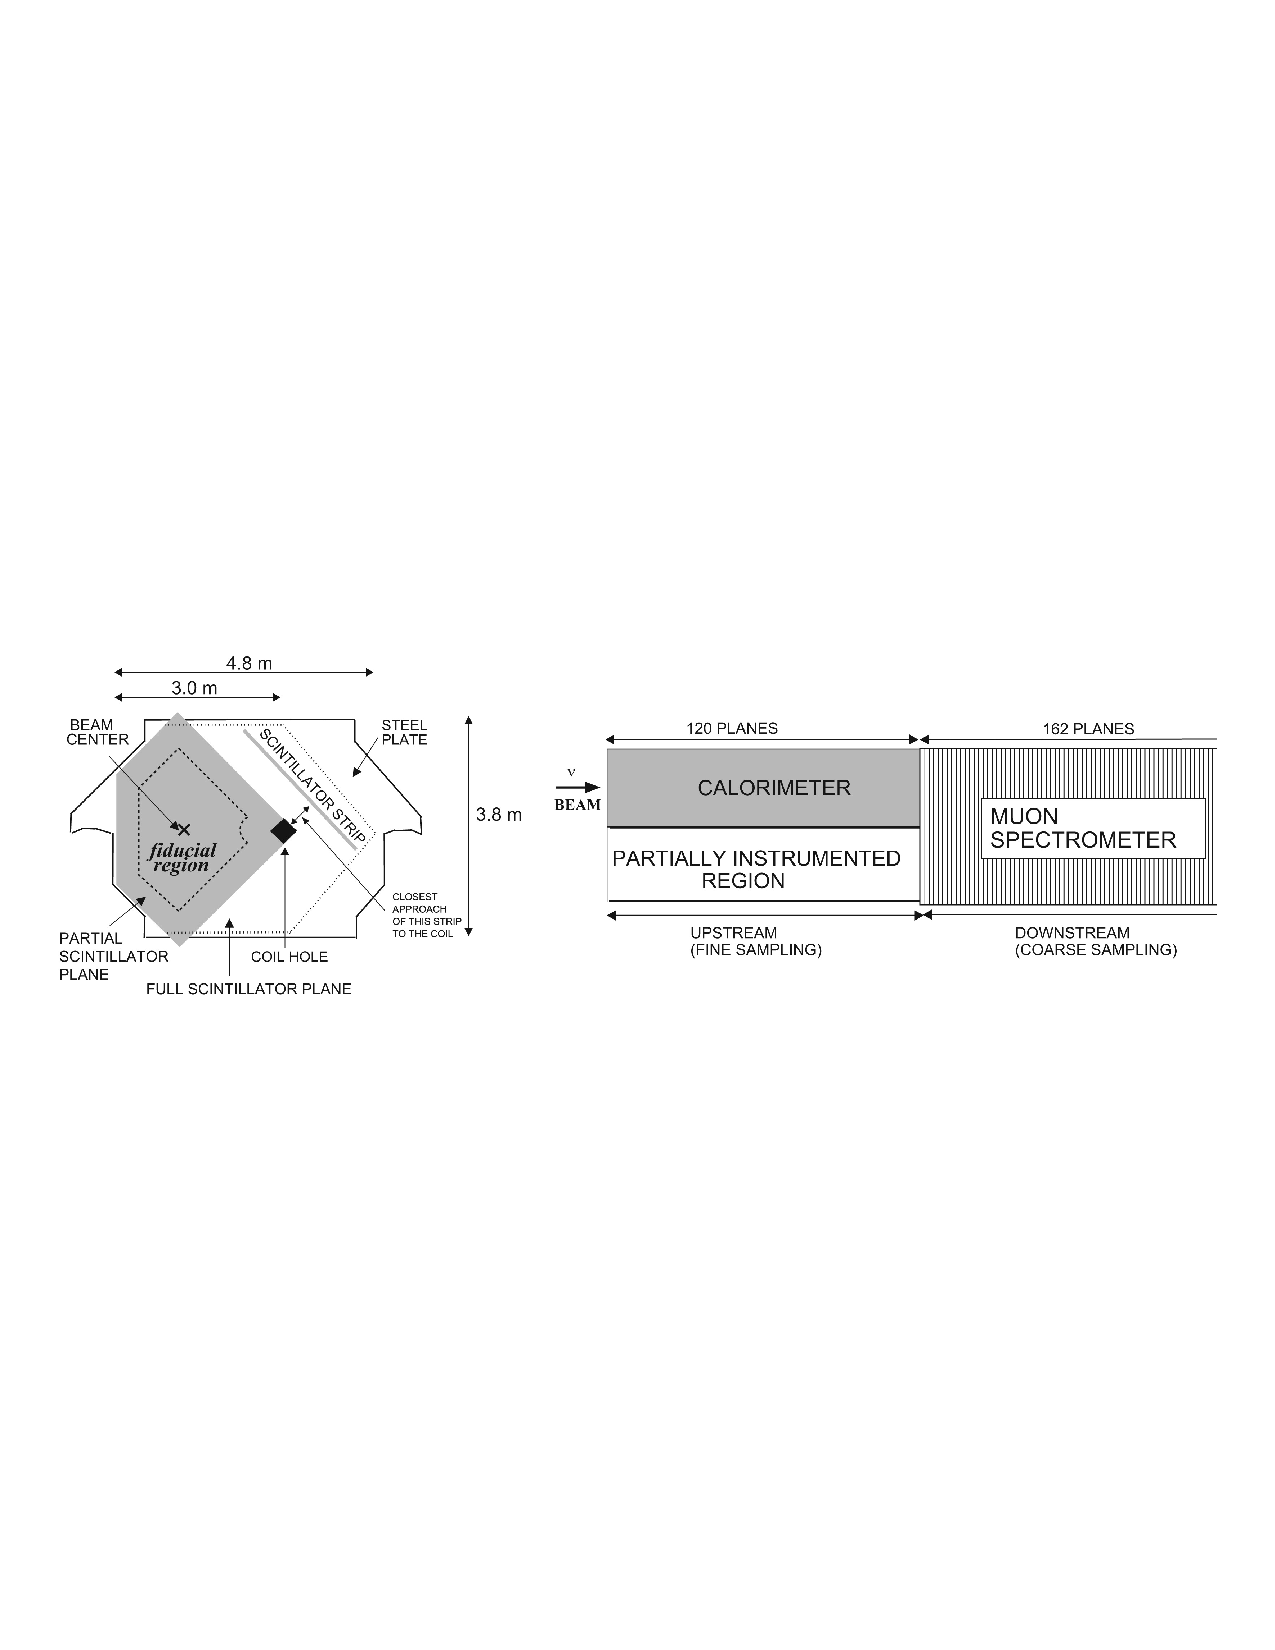
\includegraphics[width=1.\textwidth]{03minerva/figures/minos.pdf}}%
    \caption{Schematic view of the MINOS near detector. Left: Transverse view of the plane configuration looking downstream. The shaded area shows a partially instrumented active scintillator plane while the dotted line shows the outline of a fully instrumented scintillator plane. The black square represents the coil hole. Right: Top view of the MINOS near detector showing the partially instrumented calorimeter region and the muon spectrometer. Note that the partially instrumented region has a full coverage every fifth plane (like the muon spectrometer). Reprinted with permission from the MINOS collaboration \cite{PhysRevD.81.072002}. Copyright (2024) by the American Physical Society.}
    \label{fig:minos}
\end{figure}


While the design of the MINERvA detector allowed for tracking low-energy charged particles, the majority of GeV-scaled (anti)muons produced in charged-current interactions were not contained within the detector. Therefore, the physics program of the MINERvA experiment relied on the MINOS near detector shown in Figure~\ref{fig:minos} \cite{minos_MICHAEL2008190}, which was positioned 2~metres downstream of the MINERvA detector's hadron calorimeter. Crucially, although somewhat similar in design to the MINERvA HCAL, the MINOS near detector was magnetised, i.e. acting as (anti)muon spectrometer. This setup enabled precise momentum reconstruction of (anti)muons exiting the MINERvA detector volume in the forward direction.

The MINOS near detector \cite{minos_MICHAEL2008190} was a sampling calorimeter consisting of alternating planes of magnetised steel and segmented plastic scintillator, oriented in two different views to enable 3D reconstruction. The toroidal magnetic field of approximately 1.3~T was generated by a current-carrying coil spanning the entire length of the detector, as depicted in Figure~\ref{fig:minos}. Surrounding the coil, there was also a small region without the scintillator rendering this region effectively dead, which is not shown in the schematic. This aspect motivates part of the selection in this measurement, as discussed later on in Chapter~\ref{ch:analysis1D}. The optical readout system used the same PMTs as MINERvA. 

As a~charged \mbox{particle--—whether} it be an antimuon or a muon, aligning with MINERvA's scope of interest--—travelled through MINOS, it was deflected by the magnetic field. The momentum of the (anti)muon was then determined using the range and curvature of the track, while the direction of the curvature was used to specify its charge, i.e. whether it was a muon or an antimuon \cite{ospanov2008measurement}. In the context of this work, the latter is important for background removal from neutrinos produced in the antineutrino-dominated beam mode. A more detailed discussion about the reconstruction by range and curvature is included in Chapter~\ref{ch:Reconstruction}.

Considering the position and transverse dimensions of the MINOS detector relative to the MINERvA detector, the angular coverage of (anti)muons was constrained.~Specifically, (anti)muons generated as far upstream as the nuclear target region relevant for this measurement were reconstructed only if they were produced within a maximum angle of~17$^\circ$ relative to the beam. This is later demonstrated in Section~\ref{ch:efficiency}.



\chapter{Nuclear dependence of antineutrino cross-section}

%It enables a direct comparison of the impact of nuclear effects on antineutrino scattering, as well as the strong dynamics of the nucleon and nucleus that affect these interactions. 
\vspace{-10pt}
\label{ch:measurement}
This thesis presents the first high-statistics simultaneous measurement of charged-current inclusive muon antineutrino differential cross-sections on carbon, hydrocarbon, iron, and lead as a function of antimuon transverse momentum $p_{\text{T}}$ and Bjorken $x$. Inclusive analysis in this case refers to an analysis considering all final states, i.e., all antineutrino interaction modes. The measurement uses data taken by the MINERvA experiment with peak antineutrino energy of~$\sim$6~GeV. It enables a direct comparison of the impact of nuclear effects in antineutrino scattering since the cross-sections are extracted employing identical techniques, within the same detector, and with the same antineutrino beam. Additionally, this measurement expands the antineutrino data sets, which are crucial for studying CP violation. 

This chapter focuses on the specific motivation for such measurement, as well as the general process of extracting the cross-section in the variables of interest. The data and the simulation sample, their reconstruction, and the analysis procedure itself are detailed in the subsequent chapters.


\section{Motivation for the measurement}

In 2014, MINERvA presented its first EMC-like measurement of inclusive charged-current neutrino scattering on carbon, hydrocarbon, iron and lead taken during the low-energy regime with peak neutrino energy of $\sim$3~GeV \cite{Tice_PhysRevLett.112.231801}. The cross-section ratios of iron-to-hydrocarbon and lead-to-hydrocarbon as a function of reconstructed Bjorken $x$ are shown in Figure~\ref{fig:emcLike}, exhibiting relative depletion at low $x$ and enhancement at large $x$, neither of which are predicted by the simulation prediction. These discrepancies increase with the size of the nucleus. At low $x$, the result suggested that the shadowing model based on charged-lepton scattering used in the prediction does not capture the shadowing in neutrino scattering well, and larger suppression may be required. The disagreement at high~$x$ was ascribed to the omission of multi-nucleon processes such as 2p2h in the simulation prediction.

\begin{figure}[b!]
    \centering
    \vspace{-5pt}
    {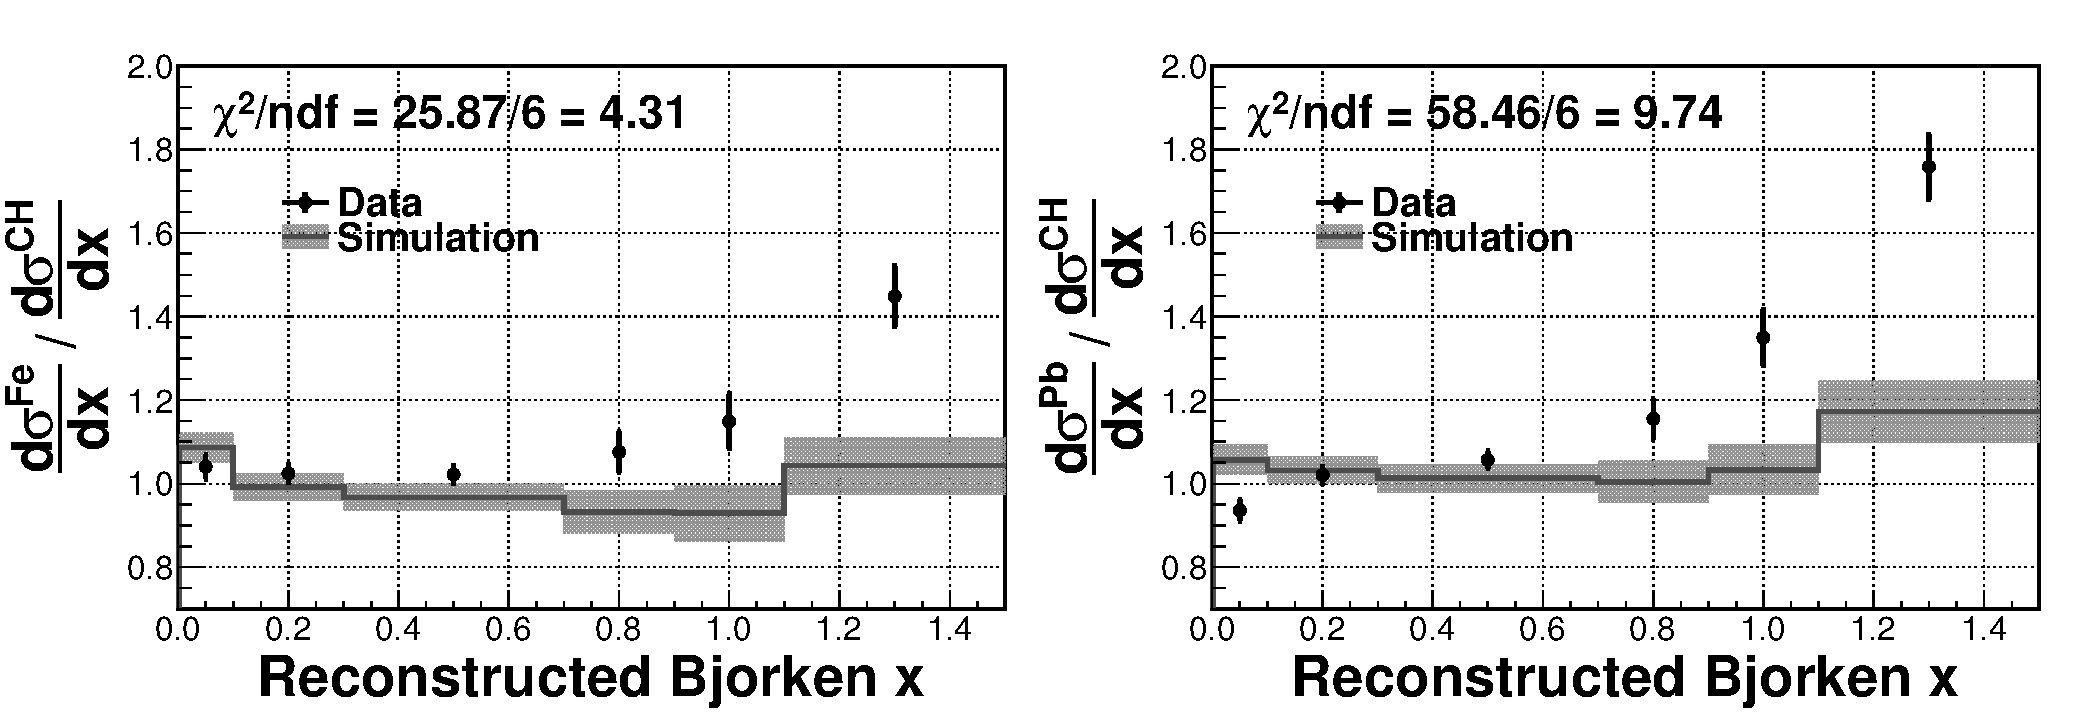
\includegraphics[width=1\textwidth]{04measurement/figures/emcLike.pdf}}%
    \vspace{5pt}
    \caption{MINERvA's measurement of iron-to-hydrocarbon (left) and lead-to-hydrocarbon (right) ratios of inclusive charged-current neutrino cross-sections per nucleon as a function of reconstructed Bjorken $x$. Reprinted with permission from Ref.~\cite{Tice_PhysRevLett.112.231801}. ~Copyright (2024) by the American Physical Society.}
    %[short caption] {long caption}
    \label{fig:emcLike}
\end{figure}

At the time, a similar analysis for inclusive antineutrino cross-section on different nuclear targets was impossible due to low statistics of antineutrino interactions in the low-energy sample. However, as a result of the long period of antineutrino operation of the NuMI beam in medium energy, MINERvA collected a high-statistics sample of antineutrino interactions that enables such investigation. Furthermore, the underlying simulation used in the measurement has undergone several improvements such as including the multi-nucleon scattering, possibly impacting the prediction for the high $x$ region. The full description of the simulation prediction used in the measurement presented in this thesis is included in Chapter~\ref{ch:dataAsimulation}. In addition, this analysis also benefits from improvements in the reconstruction of the interaction vertex crucial for distinguishing on which nucleus the interaction occurred, which are further elaborated on in Chapter~\ref{ch:Reconstruction}.

Notably, the 2014 neutrino analysis was also reported in terms of the reconstructed Bjorken~$x$ due to the inability to deconvolute the detector effects from the measurement \cite{TiceThesis2014}. Thanks to improvements in interaction modelling, reconstruction techniques, increased statistics in the sample, and rigorous unfolding studies (detailed in Section \ref{sec:migration_unfolding}), this medium-energy antineutrino analysis can now estimate the cross-section in terms of the true Bjorken $x$. This allows for reporting a detector-independent cross-section, which is valuable for interpretation in the context of various theoretical and phenomenological studies, as well as for comparisons with results from other experiments. Furthermore, the results are also reported in terms of the well-reconstructed antimuon transverse momentum $p_{\text{T}}$, which can be related to the four-momentum transfer squared in the interaction. 

% SRC

\begin{figure}[t!]
    \centering
    {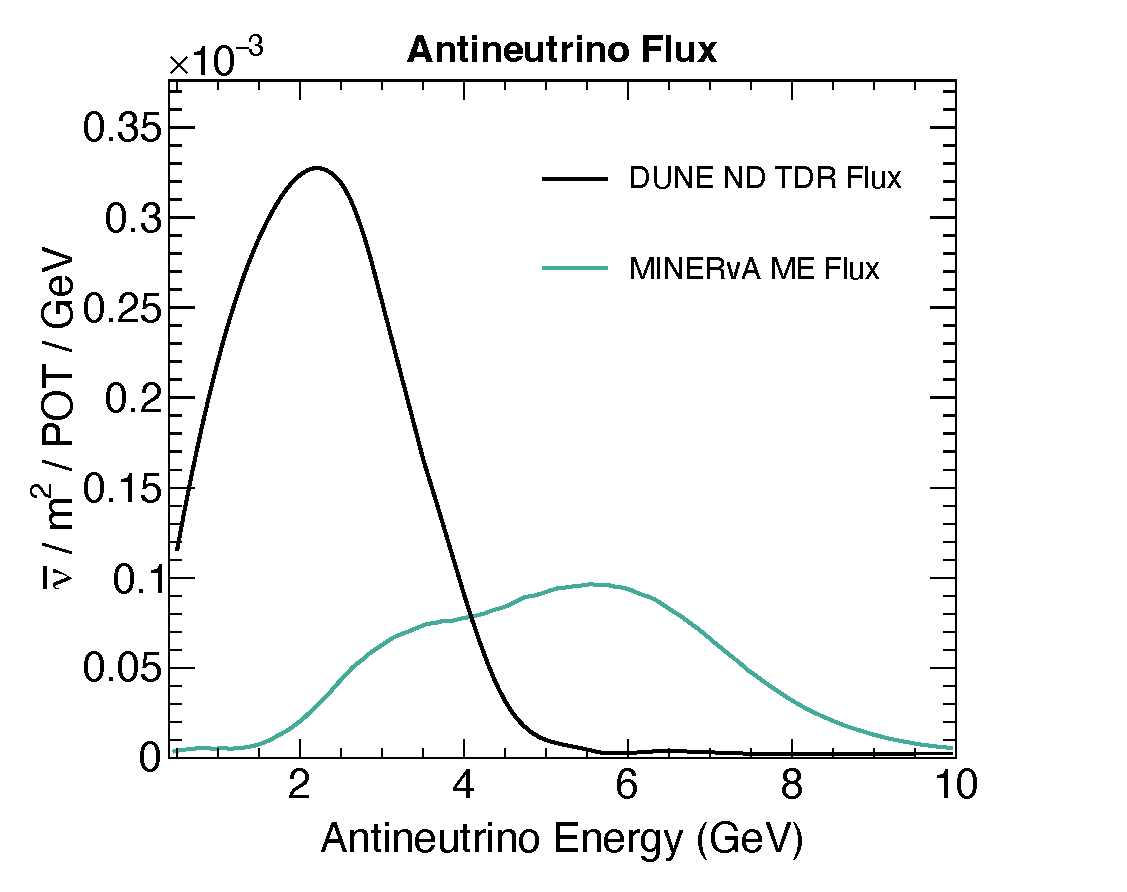
\includegraphics[width=0.75\textwidth]{04measurement/figures/antinu_flux.pdf}}%
    \caption{Comparison of the expected antineutrino flux at the DUNE near detector~(ND) according to ND Technical Design Report (TDR)~\cite{abi2020deep} and the MINERvA medium energy antineutrino flux in the 0--10 GeV range of antineutrino energy.~Note the significant overlap at the upper end of antineutrino energy.}
    %[short caption] {long caption}
    \label{fig:fluxDune}
\end{figure}

Due to the kinematic phase space spanned by the MINERvA medium energy dataset, the measurement presented in this work is predicted to be dominated by the resonant pion production, deep inelastic scattering, and the transition region between these two interaction modes, i.e. the shallow inelastic scattering. Understanding of the (anti)neutrino interactions and the nuclear effects in this energy regime is particularly important for the future oscillation experiment DUNE. This is demonstrated in Figure~\ref{fig:fluxDune} showing the expected antineutrino flux seen by the DUNE near detector compared to the MINERvA medium energy antineutrino flux utilised in this analysis, with a significant overlap corresponding to the energies where these higher-energy interaction modes are expected (cf. Figure~\ref{fig:totalXsecEnu} in Chapter~\ref{ch:theory}). 

Importantly, the (anti)neutrino scattering in DUNE will occur primarily on argon \cite{abi2020deep}. While experiments measuring (anti)neutrino cross-sections on argon exist, e.g. MicroBooNE~\cite{Acciarri_2017}, they generally probe lower-energy regions dominated by the quasi-elastic scattering. MINERvA is the only experiment that can provide direct high-statistics measurements of nuclear dependence across various nuclei in the kinematic regime dominated by these higher-energy interaction modes. Therefore, MINERvA measurements, including this one, are crucial for refining our understanding and modelling of the impact that nuclear effects have on these interaction modes, enabling the interpolation to interactions on argon. The NOvA experiment \cite{NOVA_2005nova} is also able to study these interaction channels at slightly lower energies but on a scintillator only. 

More generally, this antineutrino measurement also expands the available antineutrino datasets in the energy regime relevant to the oscillation experiments, aiding in the refinement of antineutrino interaction modelling necessary for CP violation searches. Large antineutrino datasets are somewhat rare compared to their neutrino counterparts \cite{Workman:2022ynf}, primarily due to the extended time required for collecting antineutrino scattering data. This stems from the production process of the antineutrino beam, where negatively charged pions (that decay to antineutrinos) are less likely to be produced from the protons-carbon interactions \cite{numi2016_ADAMSON2016279}. Additionally, antineutrino cross-sections are lower than those for neutrinos, as shown in Figure~\ref{fig:totalXsecEnu}.



, and they predominantly span either the quasi-elastic (e.g. T2K) or the very high-energy deep inelastic region \cite{Workman:2022ynf}. %Measurements in the $1$ GeV $<E_\bar{\nu}> < 10 $ GeV have been made by for example by MINOS on iron, 
% https://pdg.lbl.gov/2023/reviews/rpp2022-rev-nu-cross-sections.pdf

\begin{figure}[t!]
    \centering
    {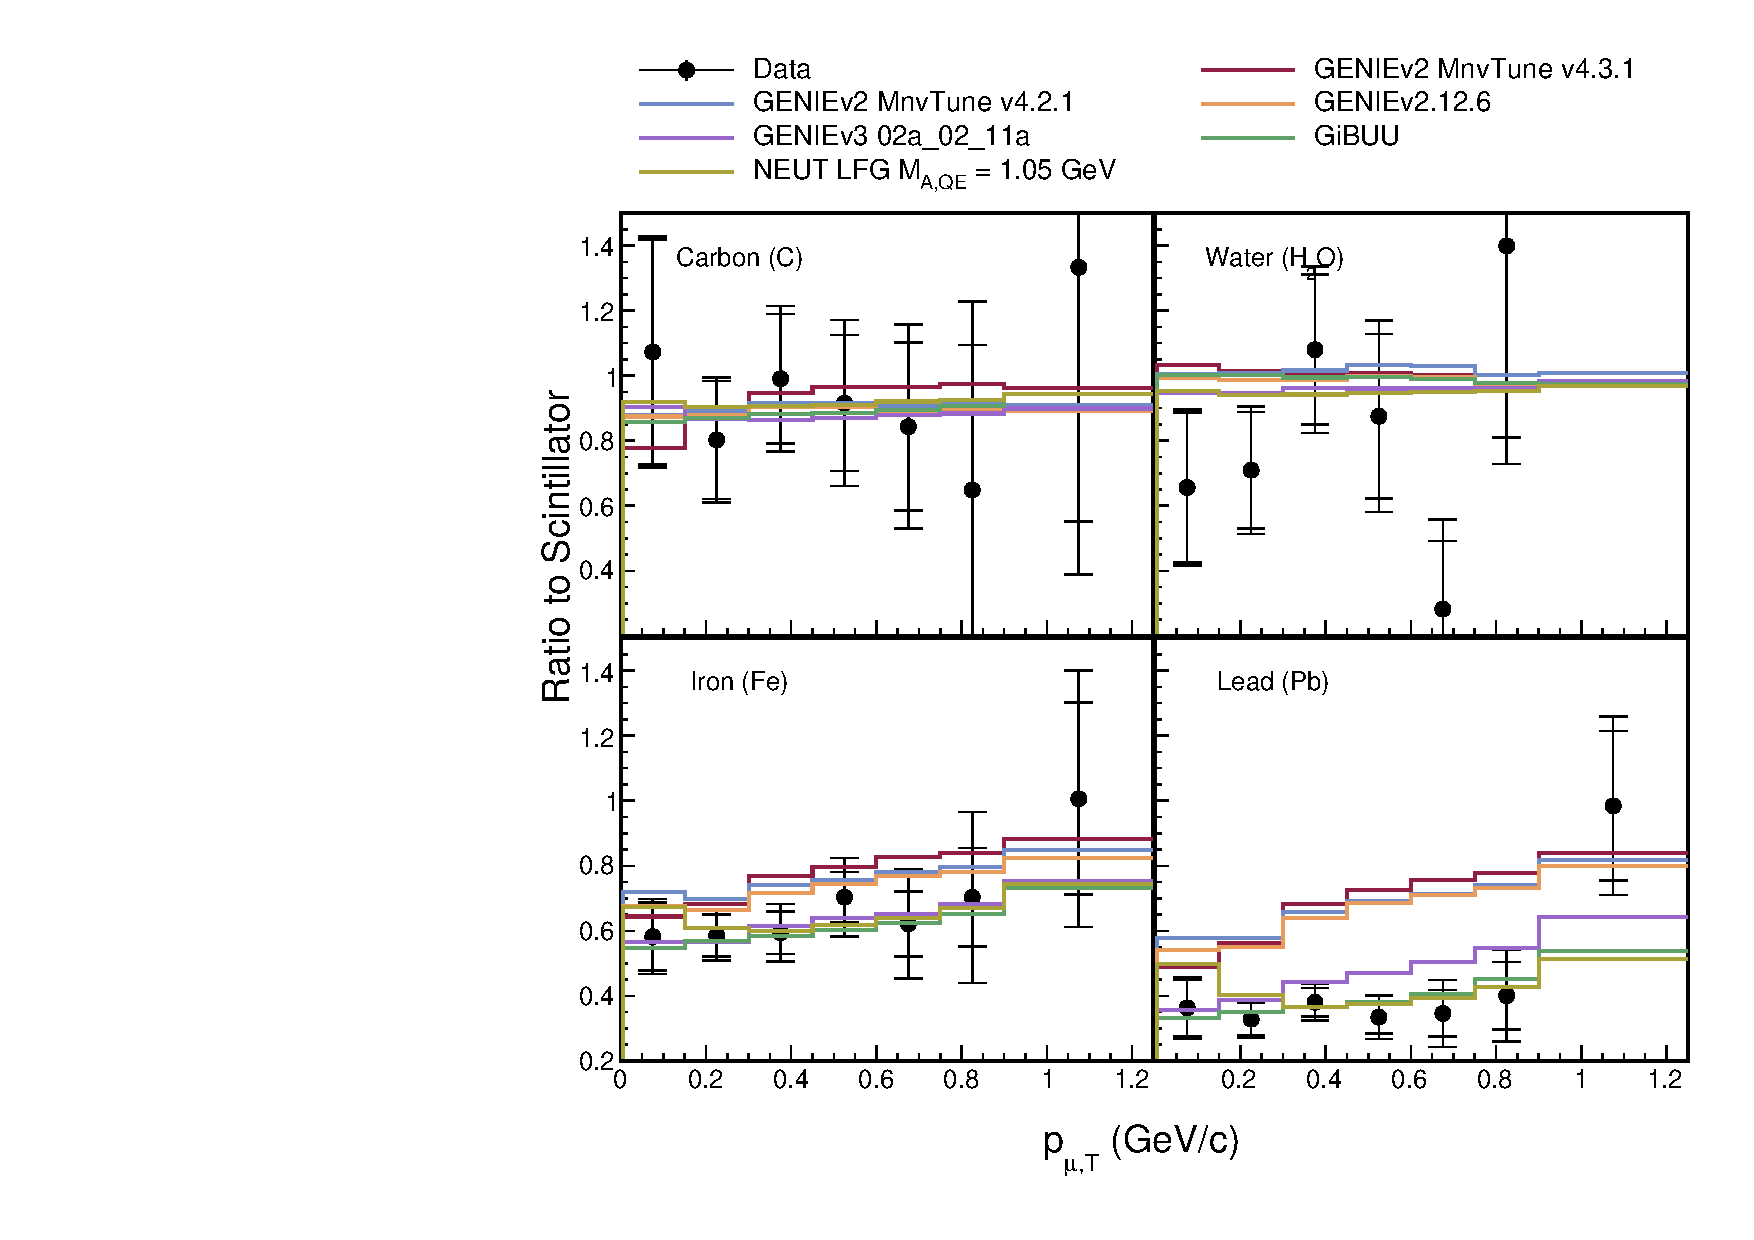
\includegraphics[width=0.8\textwidth]{04measurement/figures/aaronCC1pi.pdf}}%
    \vspace{5pt}
    \caption{MINERvA measurement of cross-section ratios for carbon, water, iron, and lead to the scintillator, i.e. hydrocarbon, for neutrino-induced charged-current single $\pi^+$ production in medium energy as a function of muon transverse momentum $p_{\text{T}}$ compared to various neutrino simulation predictions. Note that all of them are discrepant for either one or more nuclei with data showing low $p_{\text{T}}$ ($\sim Q^2$) suppression increasing with the size of the nucleus compared to the underlying simulation indicated by GENIEv2 MnvTune v4.3.1. Reprinted with permission from Ref.~\cite{Bercellie2023_PhysRevLett.131.011801}.~Copyright (2024) by the American Physical Society.}
    %[short caption] {long caption}
    \label{fig:aaronCC1pi}
\end{figure}

Finally, due to the dominant contribution from the single-pion production channel, this analysis allows for an inclusive investigation of the behaviour observed in MINERvA's measurement of neutrino-induced single-pion production across various nuclei \cite{Bercellie2023_PhysRevLett.131.011801}, as shown in Figure~\ref{fig:aaronCC1pi}, but in the antineutrino mode. 

% minerva medium energy of CC1pi + showed need for strong suppression at low Q^2 of
% this analysis enables its study in antineutrino mode


\section{How to measure the cross-section}
\begin{comment}

- MINERvA's medium energy analysis of charged-current single pion production showed a need for large suppression at low Q^2 
- see the need for a suppression of the
pion production prediction at low 𝑄2.

minerva run completed, but data continues to be analysed 
measurements help improve theoretical interaction models, essential components of neutrino oscillation programs
\end{comment}

The probability that a certain interaction process occurs is parameterised as a cross-section and can be thought of as the effective area subtended by the target particle to an incident beam \cite{perkins_2000}. This measurement reports flux-integrated differential cross-sections per nucleon on particular nuclei, namely carbon, hydrocarbon, iron, and lead. The cross-section distributions are discretised into a finite number of bins of a quantity of interest, defined in order to obtain a statistically significant sample in each of them, and are extracted as follows,
\begin{equation}
    \label{eq:xsec1D}
    {\left(\frac{d\sigma}{dx}\right)}_{\alpha} = \frac{\Sigma_{j} \tilde{U}_{j\alpha}(N_{\text{data}, j} - N^{\text{bkg}}_{\text{data}, j})}{E_{\alpha} T_{\text{nucleons}} \Phi \Delta x_{\alpha} \text{POT}} \hspace{2pt}.
\end{equation}

In the above, the left-hand side corresponds to the cross-section in bin $\alpha$ with respect to a quantity $x$. In this analysis, this quantity can either be antimuon transverse momentum $p_{\text{T}}$ or Bjorken~$x$.~To distinguish between the true value of the variable of interest, in which the final detector-independent cross-section is reported, and its reconstructed value, the bin containing the true value is labelled as $\alpha$, while the bin containing the reconstructed value is represented by $j$. The difference between the true bin and the reconstructed bin arises from the complex nature of the antineutrino interactions and the imperfect reconstruction, further explained in the following chapters.

$N_{\text{data}, j}$ is the number of reconstructed events of interest in bin $j$ and $N_{\text{data},j}^{\text{bkg}}$ is the estimated number of background events. The background-subtracted selected events correspond to the signal. Therefore, in this analysis, it is the number of all charged-current antineutrino interactions that occurred in a specific target material with certain kinematic constraints discussed in Chapter~\ref{ch:analysis1D}. $\tilde{U}_{j\alpha}$ represents the so-called unfolding process which tries to
remove the smearing of the reconstructed distribution to report the cross-section in the true quantities $\alpha$. Efficiency correction $\epsilon_{\alpha}$ takes into account the signal events that were lost due to detector acceptance and imperfect reconstruction. 

Furthermore, the differential cross-section is normalised to the flux prediction integrated over all bins, $\Phi$, the number of nucleons in a given material, $T_{\text{nucleons}}$, the bin width of the corresponding bin, $\Delta x$, to make it differential, and the number of protons on the target, POT, which is the metric used to characterize the integrated luminosity of the antineutrino beam. Note that all these individual steps of the cross-section extraction are described in detail in Chapter~\ref{ch:analysis1D}.

Finally, similar to the MINERvA analysis in Figure~\ref{fig:emclike}, the cross-section ratios of the nuclear target (A) to scintillator tracker (CH) are reported to minimise the dependence on the underlying antineutrino flux, as well as to cancel out some shared reconstruction and antineutrino interaction modelling effects. While the cross-section ratios are taken directly from the calculated cross-sections according to Equation~\ref{eq:xsec1D}, the ratios approximately correspond to
\vspace{-5pt}
\begin{equation}
    \left( \frac{d\sigma^\text{A}}{dx} \mathlarger{\mathlarger{\mathlarger{/}}} \frac{d\sigma^{\text{CH}}}{dx} \right)_{\alpha} \approx \mathlarger{\sum_j} \frac{\tilde{U}_{\alpha j}^\text{A}(N_{\text{data}, j}^\text{A}- N_{\text{data},j}^{\text{bkg},\text{A}})\epsilon_{\alpha}^{\text{CH}}T^{\text{CH}}}{\tilde{U}_{\alpha j}^{\text{CH}}(N_{\text{data}, j}^{\text{CH}}- N_{\text{data},j}^{\text{bkg},\text{CH}})\epsilon_{\alpha}^{\text{A}} T^{\text{A}}} \hspace{2pt}.
    \label{xsecs_ratios}
\end{equation}

\section{Variables of interest}

The final cross-section and cross-section ratio results are reported in terms of the antimuon transverse momentum $p_{\text{T}}$ and Bjorken $x$. The muon transverse momentum variable is well-reconstructed and can be related to the four-momentum transfer. The Bjorken x variable directly considers hadronic final states and is used to describe nuclear modifications to a bound nucleon cross-section compared to a free nucleon

How to relate

\begin{comment}

- why important
- signal definition
- other analyses
- define muon pT
- define Bjorken x
- x greater than 1 region
- why cross-section ratios
\end{comment}

\clearpage
\thispagestyle{empty}
\hfill
\clearpage
\chapter{Data and simulation samples}

\label{ch:dataAsimulation}
\vspace{-20pt}
In this measurement, I use MINERvA data collected during antineutrino-dominated medium energy (ME) physics runs with the antineutrino flux peaked near $6$ GeV, recorded between June 29th, 2016 and February 26th, 2019. The measurement utilises the minervame5A, \mbox{minervame6A--6J} `playlists', which are lists of MINERvA runs and subruns that correspond to a specific detector configuration. This amounts to the total data exposure of $1.12 \times 10^{21}$ protons on \mbox{target (POT).} 

The analysis employs Monte Carlo (MC) simulation to try to describe the underlying antineutrino interaction physics, estimate backgrounds, characterise detector inefficiencies, evaluate systematic uncertainties, and perform various other studies. It corresponds to the detector configuration of the data-taking periods described above. The simulated MC POT is equivalent to more than \mbox{$4 \times$ data POT}, i.e. $4.96 \times 10^{21}$ POT, to reduce the statistical fluctuations in the simulation. In order to compare the simulation to data, the simulation distributions are scaled by the ratio of the data POT to the simulated MC POT, so-called POT-normalised. 

The MC encapsulates the simulation of the NuMI antineutrino beam, the antineutrino interactions in the nucleus, the environment of the nucleus itself and how it affects particles exiting it, and the propagation of the final-state particles through the MINERvA detector. For further discussion in Chapter~\ref{ch:analysis1D}, it is important to emphasise that antineutrino interactions are only simulated in the nuclear targets and tracker of the MINERvA detector, excluding the electromagnetic and hadronic calorimeter.

\section{Flux simulation} \label{sec:fluxSimulation}
% say that flux simulation is described in the NuMI chapter
% in-situ measurements
% nuclear target correction
% Combined constraint: https://arxiv.org/pdf/2209.05540.pdf
% Neutrino mode: https://journals.aps.org/prd/pdf/10.1103/PhysRevD.100.092001
% IMD: https://arxiv.org/abs/2107.01059

\begin{figure}[b!]
  \centering
  {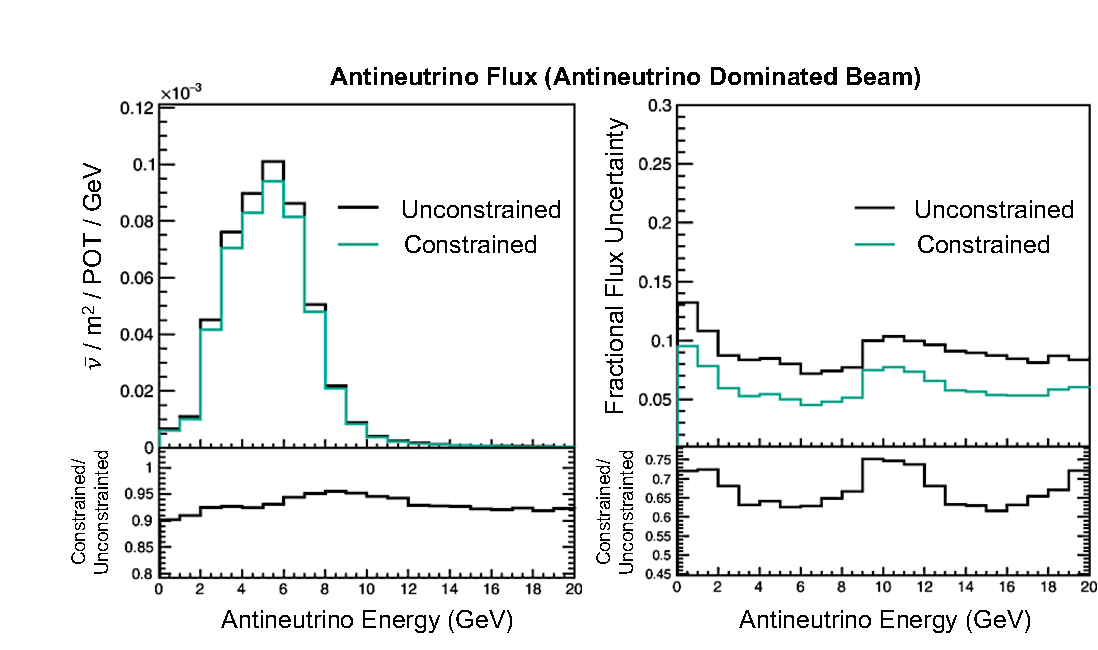
\includegraphics[width=1\textwidth]{05dataAsimulation/figures/fluxConstraint.pdf}}%
  \caption{Left: Predicted antineutrino flux in bins of antineutrino energy before and after constraining the \textit{a priori} model using the (anti)-neutrino electron scattering and inverse muon decay \textit{in-situ} measurements. Right: Fractional flux uncertainty on the predicted antineutrino flux before and after the constraint. Plots adapted from Ref.~\cite{Zazueta2023_PhysRevD.107.012001}. }
  %[short caption] {long caption}
  \label{fig:fluxConstraint}
\end{figure}
  

The simulation begins with the base antineutrino flux simulation constrained by external hadron production data described in Section~\ref{sec:NuMI}. The flux model in this analysis is further improved by \textit{in-situ} measurements of processes with known cross-sections, specifically the (anti)neutrino-electron elastic scattering \cite{Valencia2019_PhysRevD.100.092001,Zazueta2023_PhysRevD.107.012001} and inverse muon decay \cite{Ruterbories2021_PhysRevD.104.092010}.

% can be both muon neutrino (CC t-channel) and electron neutrino (NC and CC s-channel)
The (anti)neutrino-electron elastic scattering, $\nu e^{-}\rightarrow\nu e^{-}$, is a well understood, purely leptonic process. Therefore, its cross-section can be predicted to a very high precision using the Standard Model electroweak theory. The (anti)neutrino-electron elastic scattering events are relatively rare with cross-section three orders of magnitude smaller than (anti)neutrino-nucleus scattering. However, due to their distinct experimental signature of very forward electromagnetic showers with no other activity, they can be selected with only a few background events.\enlargethispage{2\baselineskip}~The discrepancies between the data and MC in the electron energy spectrum can be interpreted as mismodelling of the flux distribution, providing a constraint on the normalisation of the flux and thus the peak of the flux.~MINERvA measured the (anti)neutrino-electron elastic scattering electron energy spectra in both ME neutrino and antineutrino dominated beams physics runs \cite{Valencia2019_PhysRevD.100.092001,Zazueta2023_PhysRevD.107.012001}. 

The inverse muon decay (IMD), $\nu_{\mu}e^{-}\rightarrow\mu^{-}\nu_{e}$, is another leptonic process which was measured by MINERvA in order to constrain the flux \cite{Ruterbories2021_PhysRevD.104.092010}. It can be identified by a very forward-going high-energy muon. IMD has (anti)neutrino energy threshold of \mbox{$\approx 11$ GeV}. Hence, it provides insight into the high-energy tail of the flux, in which phase space is mostly dominated by (anti)neutrinos produced by underfocused or unfocused $K^+$ \mbox{and $\pi^{+}$}. 

This analysis uses MINERvA's combined flux constraint of (anti)neutrino-electron scattering and IMD \cite{Zazueta2023_PhysRevD.107.012001} whose impact is shown in Figure \ref*{fig:fluxConstraint}. The single normalisation constraint was extracted using Bayes' theorem, where the posterior probability is given by the prior flux prediction multiplied by the likelihood of the electron spectra measurement given the \textit{a priori} model. The \textit{a priori} flux uncertainty is estimated using the multiverse method \cite{MAT_Messerly_2021}, where an ensemble of flux predictions, so-called universes, is created by varying flux parameters within their uncertainties. The procedure takes into account the correlations between the predictions of the number of events. 

The flux simulation is then reweighted by the ratio of the weighted average of post-constraint flux universes to the weighted average of pre-constraint fluxes. The procedure results in predictions from universes with poor data agreement to be weighted down, which reduces the uncertainty (spread of the universes). In antineutrino dominated beam, the antineutrino energy range integrated flux uncertainty is reduced from $7.8\%$ to $4.7\%$ \cite{Zazueta2023_PhysRevD.107.012001} as shown in Figure \ref*{fig:fluxConstraint} and is further discussed in Chapter~\ref{ch:systematics}.

\subsection{Nuclear target flux} \label{sec:nuclear_target_flux}

% Figures:
% calculated flux in targets + ratio (antineutrinos)
% point to neutrinos in a reference
% Flux in individual petals figure
% Figure of the individual petals in a hexagon
% Regularisation curve for targets in the back-up
% back-up: antineutrino energy flux in 2D rebinning
% weights before and after in the back-up for carbon, maybe get others 
% table of chi2 in the back-up

While the antineutrino beam is focused as described in Section~\ref{sec:NuMI}, the transverse distribution of the beam is relatively wide. Additionally, due to the downward pointing of the NuMI beam with respect to MINERvA, this also affects the flux seen by the detector as a function of the longitudinal position.\enlargethispage{1\baselineskip} The flux distribution described above provides an accurate representation of the averaged flux in the active tracker region and correctly accounts for these effects. However, the complex geometry of the nuclear target region, as detailed in Section~\ref{sec:MINERvAdetector}, with varying transverse positions of different materials within individual targets, particularly off-centre of the detector and, consequently, off-centre of the beam, is expected to introduce variations in both shape and normalisation of the flux compared to the tracker.

The nuclear target flux differences in the neutrino beam were first taken into consideration in cross-section calculations in Refs.~\cite{KleykampThesis2021, KleykampCCQE_PhysRevLett.130.161801} with applied neutrino-electron elastic scattering flux constraint only. To enable flux-independent comparisons between nuclear targets, i.e.~the nuclear target-to-scintillator cross-section ratios as discussed in Chapter~\ref{ch:measurement}, the procedure in Refs.~\cite{KleykampThesis2021, KleykampCCQE_PhysRevLett.130.161801} extracts the scintillator tracker cross-section in different transverse regions of the MINERvA fiducial volume. It is then weighted so that the summed scintillator cross-section has the same effective flux as the target flux.

\begin{figure}[b!]
  \centering
  \vspace{5pt}
  {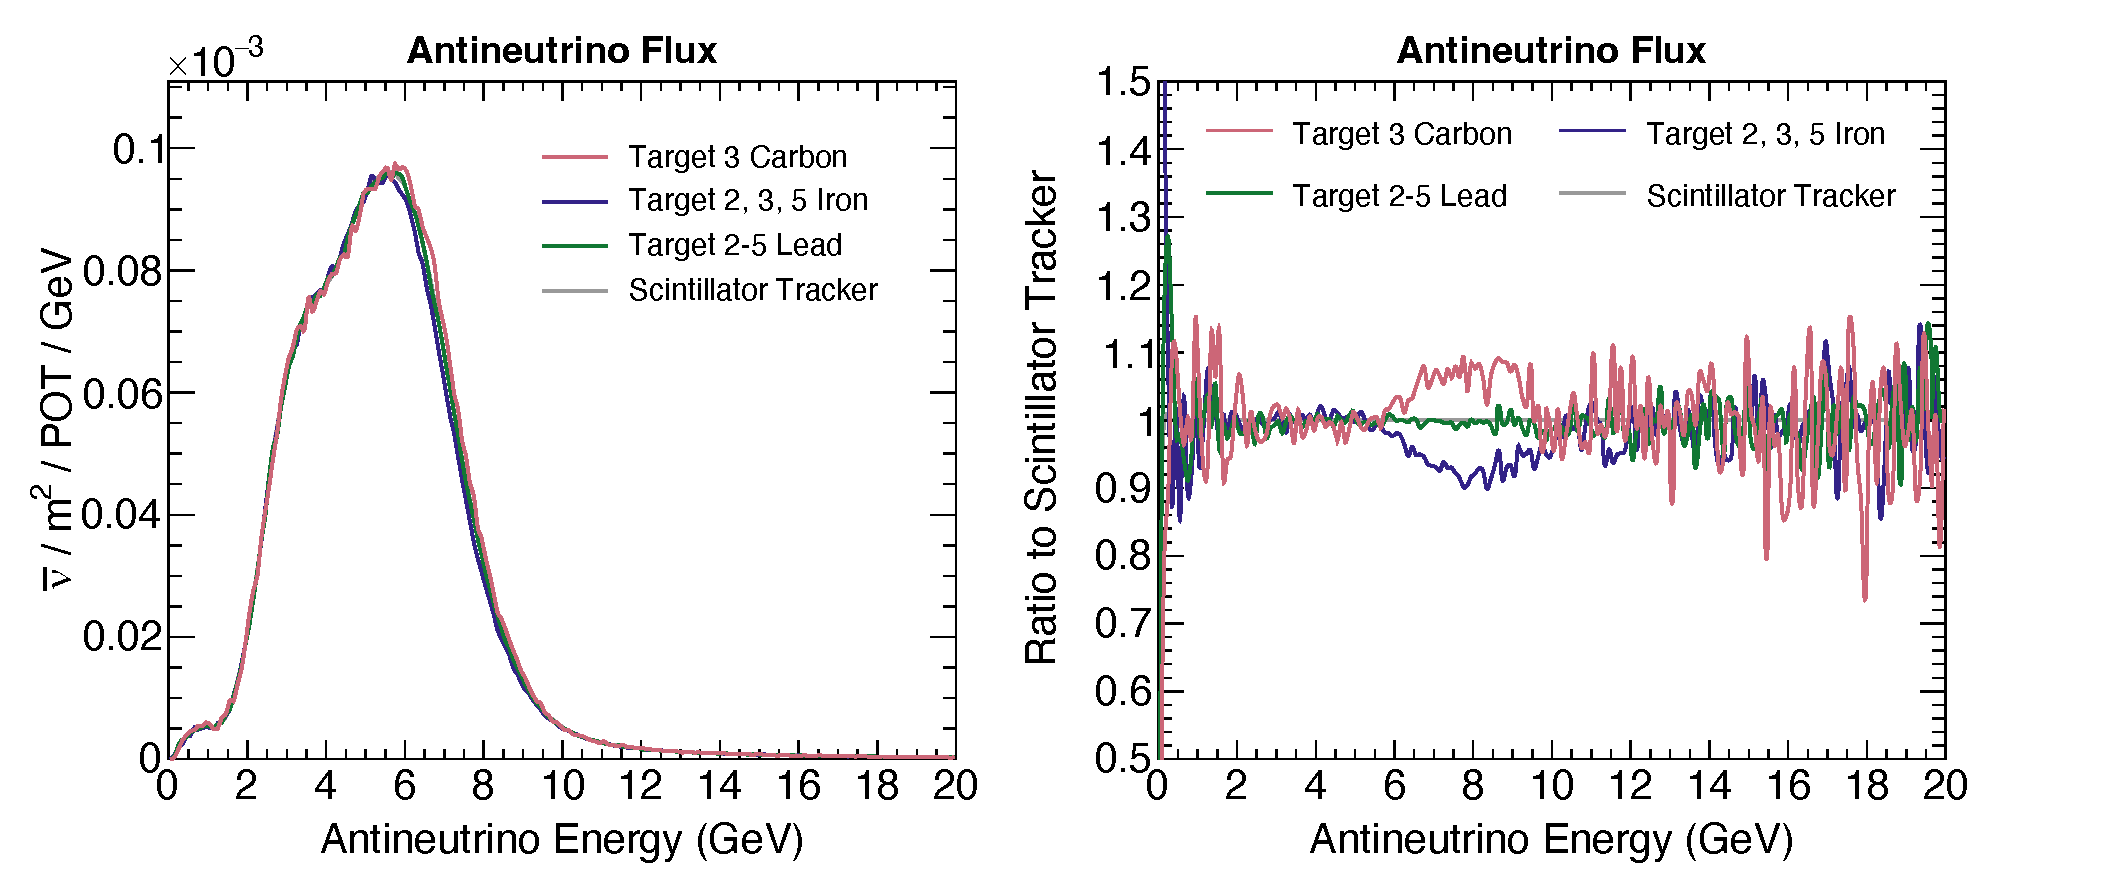
\includegraphics[width=1.01\textwidth]{05dataAsimulation/figures/nuclearFlux.pdf}}%
  \caption{Left: Calculated antineutrino flux for carbon, iron, and lead compared to the scintillator tracker flux. Right: Nuclear target-to-scintillator tracker flux ratio illustrating the flux differences in the 6--10~GeV region.}
  %[short caption] {long caption}
  \label{fig:nuclearFlux}
\end{figure}

I extended the procedure to the antineutrino flux with MINERvA's combined flux constraint of (anti)neutrino-electron scattering and IMD, and simultaneously reimplemented the neutrino flux with this new flux constraint as well. The antineutrino fluxes for each nuclear target (or combined nuclear targets of the same material) were calculated, as detailed in Appendix~\ref{ch:appendix_NuclearTargetFlux}, using the true information from the simulation.\enlargethispage{1\baselineskip}

Figure~\ref{fig:nuclearFlux} depicts the calculated antineutrino fluxes for the combined nuclear targets used in this work and their ratios to the scintillator tracker flux distribution. Generally, the nuclear target fluxes differ by up to 10\% in the 6--10~GeV region (the falling edge of the flux peak). If the average position of the target is above the centre of the beam, as is the case for carbon, the nuclear target flux is higher than that for the scintillator. Conversely, if the average position of the target is below the centre of the beam, as is the case for the combination of iron targets, the nuclear target flux is lower than that for the scintillator. The combination of lead targets has approximately the same centre of mass and shape as the tracker, thus resulting in a flat lead-to-scintillator flux ratio.

\begin{figure}[b!]
  \centering
  \vspace{-10pt}
  {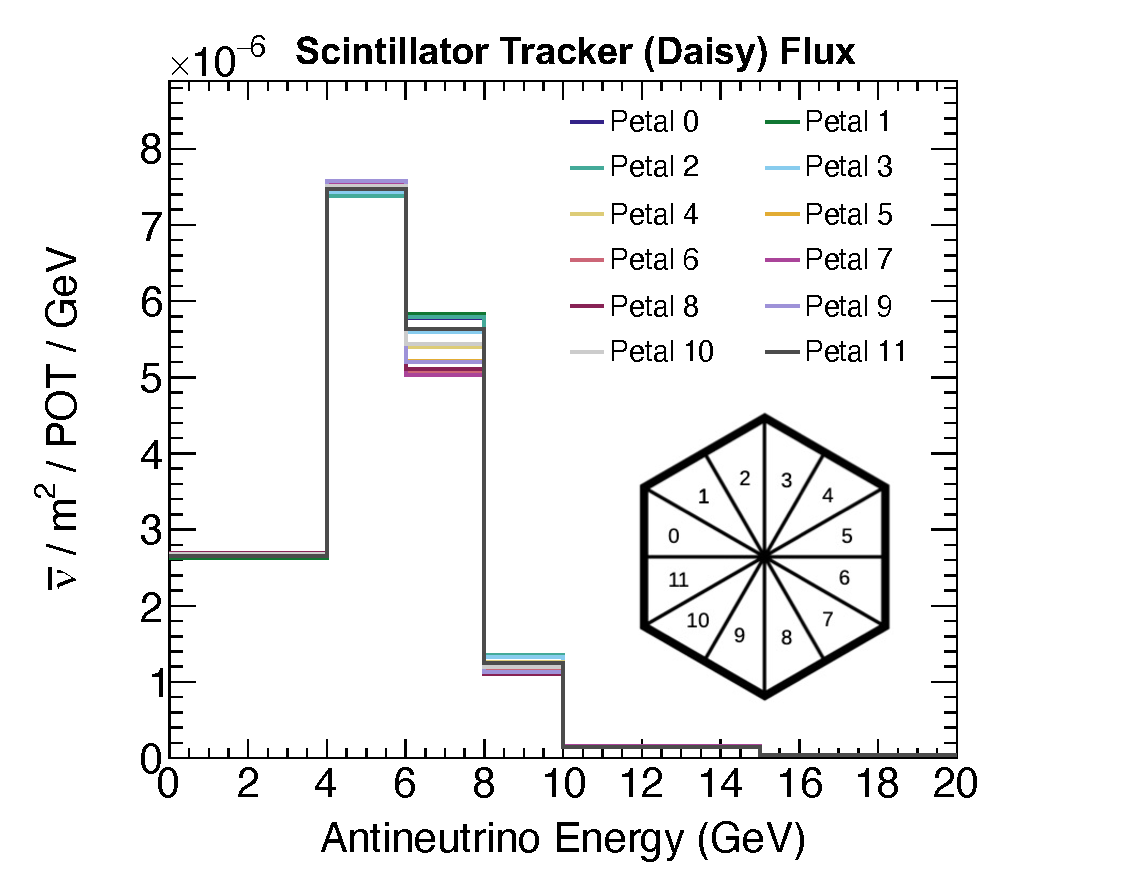
\includegraphics[width=0.8\textwidth]{05dataAsimulation/figures/daisyPetals.pdf}}%
  \caption{Antineutrino scintillator tracker flux for each ‘daisy petal' as a function of antineutrino energy. The hexagon insert illustrates petal positions when looking downstream of the detector.}
  %[short caption] {long caption}
  \label{fig:daisyPetals}
\end{figure}

Similarly to the nuclear target fluxes, the scintillator tracker flux can be extracted in~12~transverse bins referred to as ‘daisy petals', as illustrated in Figure~\ref{fig:daisyPetals}.~A~linear combination of these ‘daisy petal' fluxes is then taken to create an effective scintillator tracker flux that matches that of the nuclear target combination.\enlargethispage{1.5\baselineskip}~The weights for the individual petals are calculated using a regularised $\chi^{2}$ fit and later applied to the efficiency-corrected ‘daisy petal' distributions in the analysis procedure detailed in Chapter~\ref{ch:analysis1D}. Specifics of this so-called ‘daisy' reweight technique are also further described in Appendix~\ref{ch:appendix_NuclearTargetFlux}.


\section{Antineutrino simulation}
% MINERvA tune v4.3.0
% GENIE 2.12.5 with Valencia RPA applied to QE (RFG), non-resonant pion
% production reductuon to 43%, low recoil fit (LE) applied to Valencia 2p2h (50% enhancement integrated over phase space)
% Full pion bubble chamber fit (CCNormREs increased to 1.15 and MaRES set to 0.94 + correlations)
% CC1pi+ lowQ2 pion production syppression (ME) + normalization of COH using the angle and energy of the pion with highest kinetic energy
% - applied to resonant and DIS events with W < 1.4 GeV with single pion multiplicity - antineutrino case applied to pi- instead of pi+
% Resonant and DIS the larget contribution to the inclusive ME sample

% Nuclear model
% Interacion model
% Quasi-elastic scattering
 % Valencia RPA
% Multi-nucleon scattering
    % Valencia 2p2h 
    % LE Fit
% Pion production
  % Resonant pion production 
    % Full pion bubble chamber fit
  % Non-resonant pion production
    % Non-resonant pion production reduction
  % Coherent pion production
    % normalization
% Deep inelastic scattering
% Final state interactions

MINERvA uses the (anti)neutrino interaction event generator GENIE (Generates Events for Neutrino Interaction Experiments) version 2.12.6 \cite{genie_ANDREOPOULOS201087,genie_andreopoulos2015}. It models how often (anti)neu\-tri\-nos from NuMI interact with nuclei in MINERvA and what are the underlying interaction physics processes. It also models the nuclear environment of the nucleus and how it affects the initial (anti)neutrino interaction as well as the final-state kinematics, i.e. what particles are produced in the final state. Furthermore, this analysis uses a variety of modifications to the baseline antineutrino simulation to better describe MINERvA data. These are applied as weights to each event, effectively scaling the probability of the event occurring based on the fit to the experimental data.
% GENIE https://arxiv.org/abs/0905.2517
% GENIE https://arxiv.org/abs/1510.05494

\subsection{Nuclear model}

As the incoming antineutrino in most cases interacts with the constituents of the nucleus~(nucleons or quarks), the simulations need to account for the effects of the nuclear environment. GENIE models the nucleus as a relativistic Fermi gas (RFG) \cite{RFG_SMITH1972605}, where nucleons are confined to a potential well with walls at the nuclear radius. RFG treats the nucleons within a nucleus as independent particles (so-called impulse approximation). The nucleons inside the nucleus have a nucleus-specific flat momentum distribution between~0~and the Fermi momentum $p_{\text{F}}$ in the ground state, determined from inclu\-sive electron scattering, and binding energy $E_{\text{B}}$. The $E_{\text{B}}$ refers to the energy needed to sepa\-rate a bound nucleon from the nucleus. 

% before corrections
%needed to bring a bound nucleon on-shell and separate it from the remnant nucleus, or for the nucleus to be excited to a~higher-energy bound state. 

% RFG https://www.sciencedirect.com/science/article/pii/0550321372900405

Because nucleons are fermions, they must obey the Pauli exclusion principle resulting in Pauli blocking. In quasi-elastic interactions, the final-state nucleon has to have momentum above $p_{\text{F}}$, which significantly suppresses the cross-section at low $Q^{2}$. To account for short-range correlations between the nucleons, i.e.~interactions between the nucleons inside the nucleus, which can lead to a momentum greater than $p_{\text{F}}$, the simulation contains Bodek-Ritchie high-momentum tail \cite{BodekRitchie1981_PhysRevD.24.1400}.
% Bodek Ritchie tail https://link.aps.org/doi/10.1103/PhysRevD.24.1400

Other nuclear models are relevant in the context of certain antineutrino interaction processes and are discussed below.
%M.Martini et al. A Unified approach for nucleon knock-out, coherent and incoherent pion production in neutrino interactions with nuclei. Phys. Rev. C 80:065501 (2009).
%GENIE models the nucleus as a relativistic Fermi gas (RGF) Martini et al.

%Adapted from Carlos A. Bertulani, Nuclear physics in a nutshell,
%Princeton University Press, 2007, p. 473


\subsection{Interaction model}
As described in Chapter~\ref{ch:theory}, different types of antineutrino interactions occur at different antineutrino energies. Due to the inclusive nature of this analysis, all antineutrino interaction modes contribute to the final cross-section. However, the higher-energy inelastic components such as resonant pion production and deep inelastic scattering will be dominant in the ME sample. The antineutrino interaction model described below will be referred to as MINERvA tune v4.3.0.


\subsubsection{Quasi-elastic scattering}
Quasi-elastic interactions are simulated using the Llewellyn-Smith formalism \cite{LLEWELLYNSMITH1972261}, which factorises the cross-section as a function of the four-momentum transfer squared, $Q^2$. The quasi-elastic vector form factors are modelled using the BBBA05 parametrization~\cite{BRADFORD2006127} of the electromagnetic form factors from electron scattering experiments. The axial form factor uses the dipole form with an axial mass of $M_{A}^{\text{QE}} = 0.99$ GeV/$c^2$. In addition, MINERvA's low energy low recoil neutrino analysis shown in Figure \ref{fig:LElowRecoil_2p2hRPA} demonstrated suppression of data in the low $Q^2$ region possibly due to long-range correlations in the nucleus \cite{Rodrigues2016_PhysRevLett.116.071802}. To address this, MINERvA modifies the baseline simulation as a function of energy and three-momentum transfer based on the random phase approximation (RPA) part of the Valencia model~\cite{RPANieves2004_PhysRevC.70.055503, gran2017model}.

\begin{figure}[b!]
  \centering
  {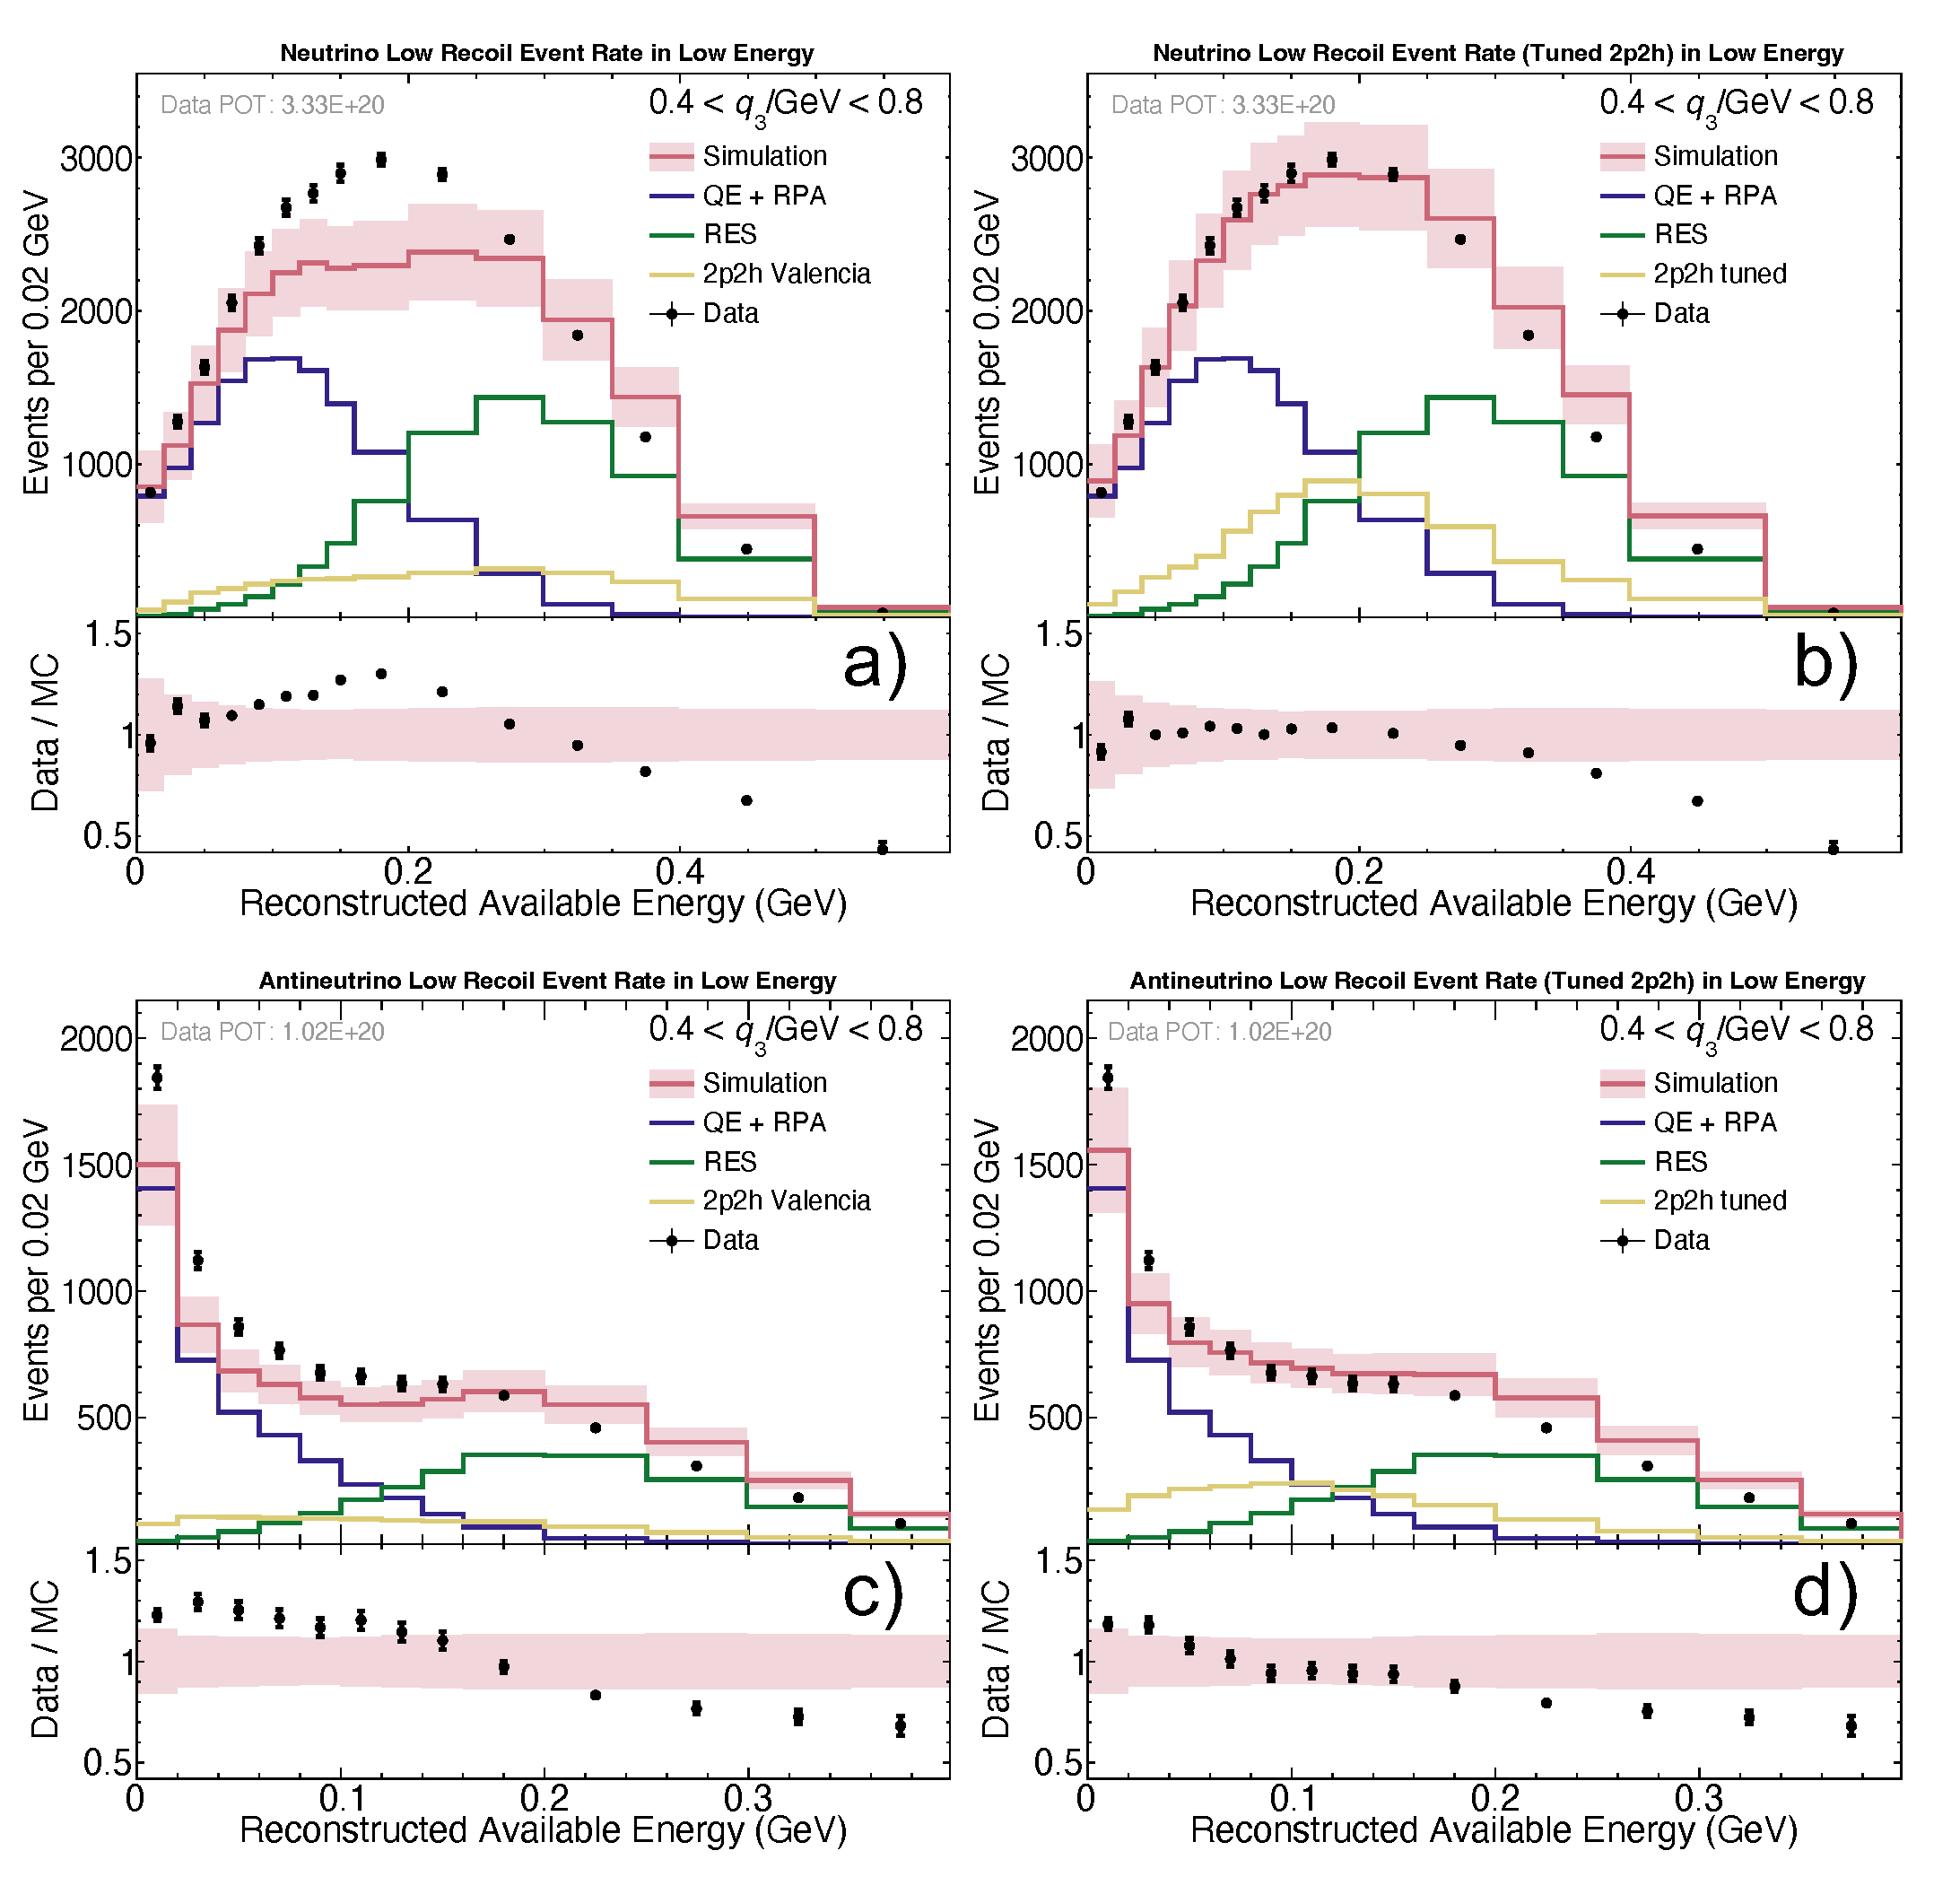
\includegraphics[width=1.01\textwidth]{05dataAsimulation/figures/LElowRecoil_2p2hRPA.pdf}}%
  \caption{MINERvA measurements of neutrino \cite{Rodrigues2016_PhysRevLett.116.071802} and antineutrino \cite{Gran2018_PhysRevLett.120.221805} low-recoil scattering in low energy as a function of reconstructed available energy, motivating the addition of RPA and 2p2h modification.~Note that the available energy corresponds to the visible recoil energy in the detector. a)~Low energy low recoil neutrino comparison of simulated and measured event rate with visible data and simulation discrepancy. b)~Improved simulation with enhanced 2p2h events shows better agreement with data. c)~Equivalent analysis in antineutrino mode compared to the base simulation. d)~Improved simulation in the antineutrino mode using the fit of the 2p2h enhancement from the neutrino mode, i.e. b), also shows better agreement with data. Furthermore, the distributions demonstrate the need for the random phase approximation (RPA) suppression in the quasi-elastic process (QE).}
  %[short caption] {long caption}
  \label{fig:LElowRecoil_2p2hRPA}
\end{figure}

% LLewellyn-Smith: https://www.sciencedirect.com/science/article/abs/pii/0370157372900105
% BBBA05: https://www.sciencedirect.com/science/article/pii/S0920563206005184
% Rodrigues: https://journals.aps.org/prl/abstract/10.1103/PhysRevLett.116.071802
% RPA Valencia model: https://arxiv.org/abs/nucl-th/0408005
% RPA Valencia model procedure: https://arxiv.org/abs/1705.02932


\subsubsection{Multi-nucleon scattering}
\label{subsec:2p2h}
Multi-nucleon scattering, specifically the 2p2h interaction, is simulated using the Valencia 2p2h model~\cite{2p2hNieves2011_PhysRevC.83.045501,2p2hGran2013_PhysRevD.88.113007,2p2hschwehr2017genie}. However, based on MINERvA's low energy recoil neutrino analysis~\cite{Rodrigues2016_PhysRevLett.116.071802}, the cross-section is increased in specific regions of energy and three-momentum transfer as shown in Figure \ref*{fig:LElowRecoil_2p2hRPA}.\enlargethispage{1\baselineskip} This results in 2p2h rate enhancement by 50\% over the nominal prediction when integrated over all phase space. Figure \ref*{fig:LElowRecoil_2p2hRPA} also shows the equivalent analysis in the antineutrino mode \cite{Gran2018_PhysRevLett.120.221805} and how the 2p2h tune (fit to neutrino data only) naturally improves the simulation prediction for the data. \vspace{20pt}



% Valencia 2p2h model: https://arxiv.org/abs/1102.2777
% Valencia 2p2h model: https://arxiv.org/abs/1307.8105
% Valencia 2p2h model in GENIE: https://arxiv.org/abs/1601.02038

% Low recoil analysis: https://journals.aps.org/prl/abstract/10.1103/PhysRevLett.116.071802
% 2p2h enahncement: https://journals.aps.org/prl/abstract/10.1103/PhysRevLett.120.221805

\subsubsection{Pion production}
\label{subsec:pionProduction}
% OG Rein-Seghal: https://www.pas.rochester.edu/~ksmcf/rein-sehgal/rein-sehgal.pdf
% GENIE documentation: https://arxiv.org/pdf/1510.05494.pdf
% How specifically imlemented and what resonances are omitted from R-S; https://journals.aps.org/prd/pdf/10.1103/PhysRevD.100.072005
% Note the resonances omitted are delta 1600 and N 1990 (quoted as 1970 in the original paper): https://pdg.lbl.gov/2011/listings/rpp2011-list-N-1990-F17.pdf
% P. Stowell's thesis is pretty good too: https://etheses.whiterose.ac.uk/22623/1/thesis.pdf

GENIE simulates the charged and neutral single pion production via baryon resonances using the Rein-Seghal (RS) model \cite{REIN198179} up to the hadronic invariant mass cut of $W$~=~1.7~GeV/$c^2$ \cite{genie_ANDREOPOULOS201087, genie_andreopoulos2015}. Out of the 18 resonances in the RS model, only 16 are included in GENIE due to $\Delta$(1600) and $N$(1990) having ambiguous experimental signatures at the time of implementation \cite{genie_ANDREOPOULOS201087, genie_andreopoulos2015}. It also does not include interference terms between the resonances and the lepton masses in the cross-section calculation. However, the effect of the latter is taken into account in calculating the phase space limits. 

%\begin{table}[ht]
%  \caption{Nonlinear Model Results}
%  \centering
%  \begin{tabular}{c c c c}
%  \hline\hline
%  Case & Method\#1 & Method\#2 & Method\#3 \\ [0.5ex] % inserts table %heading
%  \hline
%  1&50&837&970 \\
%  2&47&877&230 \\
%  3&31&25 &415 \\
%  4 & 35 & 144 & 2356 \\
%  5 & 45 & 300 & 556 \\ [1ex]
%  \hline
%  \end{tabular}
%  \label{table:nonlin}
%\end{table}

% Rein-Seghal: https://www.sciencedirect.com/science/article/abs/pii/0003491681902426?via%3Dihub
% P33 and(1640) and F17(1970) from RS model are not in GENIE: https://genie-docdb.pp.rl.ac.uk/DocDB/0000/000002/003/man.pdf p 26
% This corresponds to
% Delta 3/2 around 1630
% N 7/2 around 1970
% N has isospin of 1/2
% Delta has an isospin of 3/2

\begin{figure}[b!]
  \centering
  {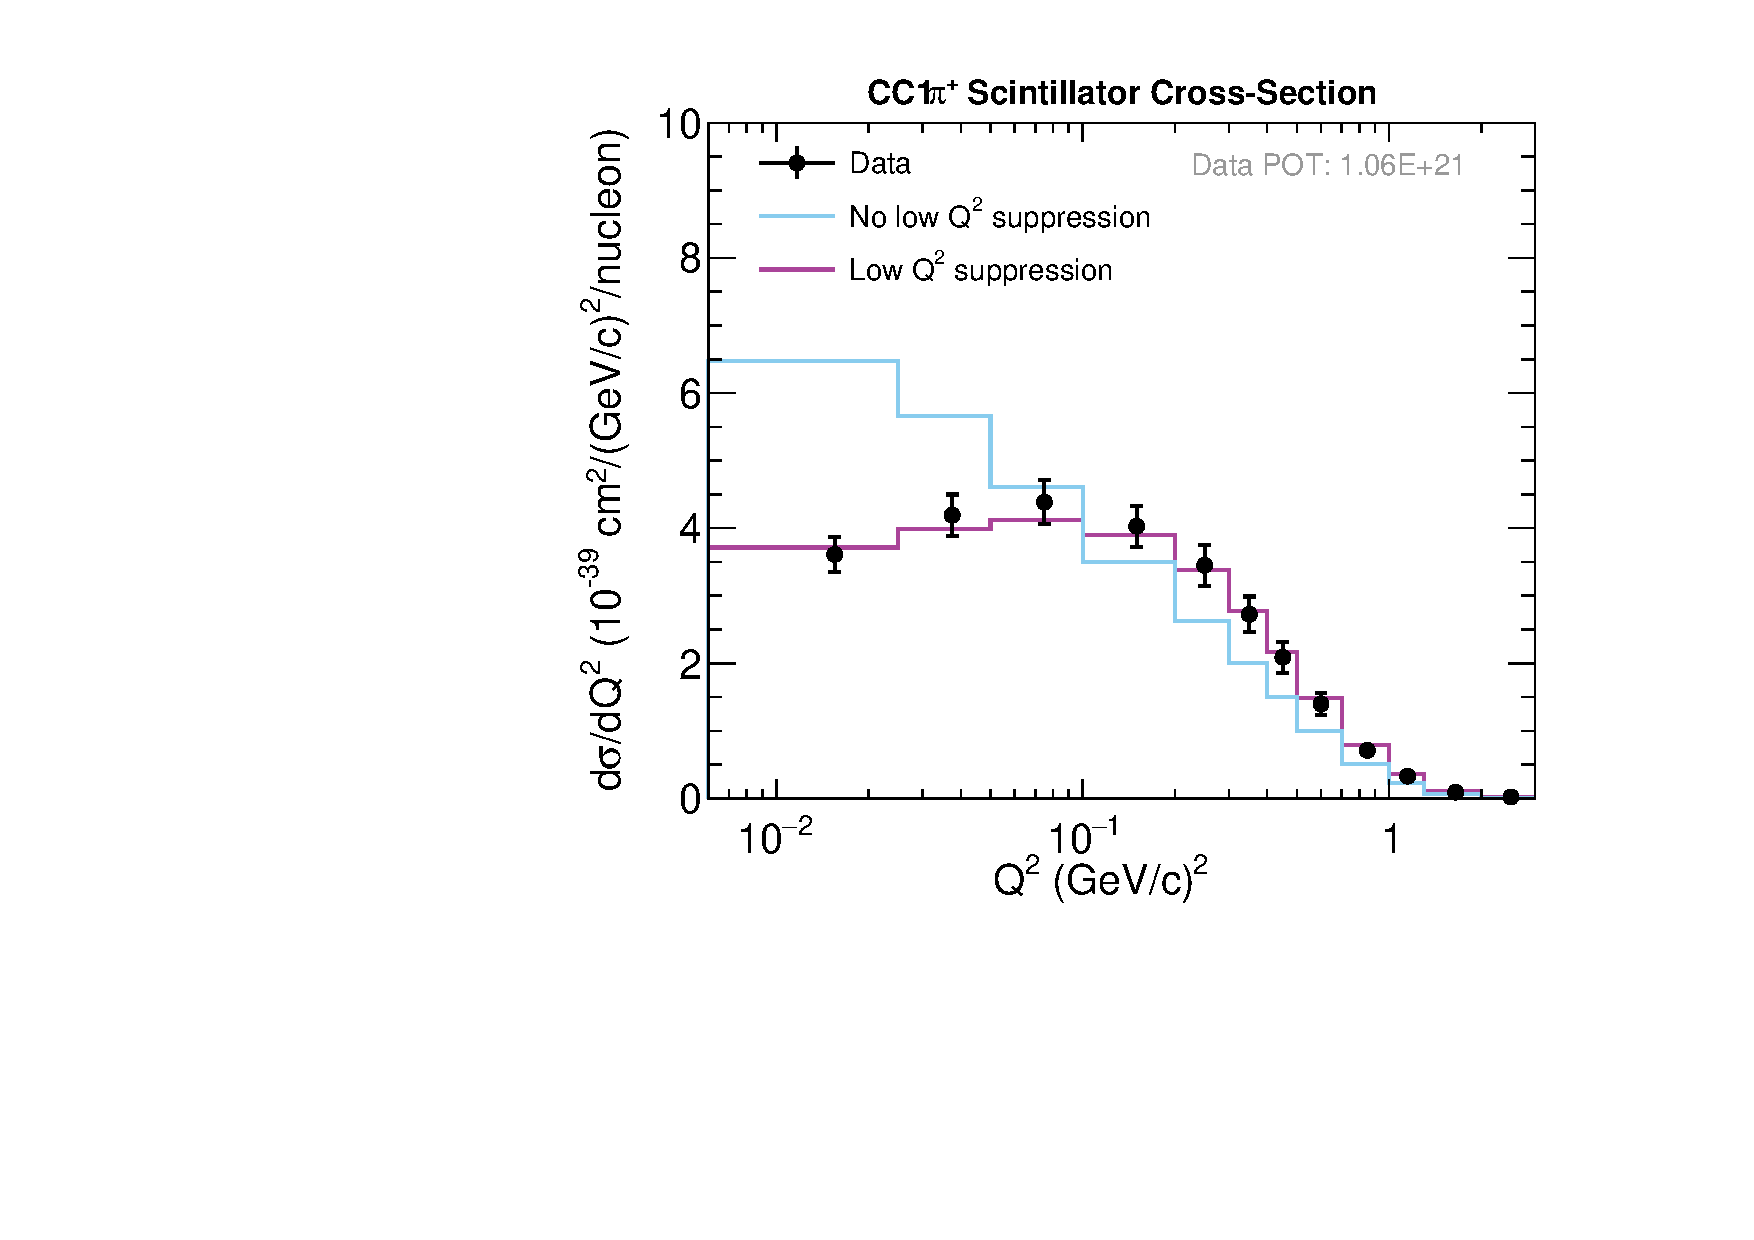
\includegraphics[width=0.8\textwidth]{05dataAsimulation/figures/lowQsup_xsec.pdf}}%
  \caption{Charged-current single pion cross-section measurement on the scintillator (data points) as a function of the four-momentum transfer squared, $Q^2$, compared to the simulation without and with the low $Q^2$ suppression. The simulated cross-section with the low $Q^2$ suppression shows better agreement with the data. Plot uses the medium energy CC1$\pi^{+} $ result \cite{Bercellie2023_PhysRevLett.131.011801}.}
  %[short caption] {long caption}
  \label{fig:lowQsup}
\end{figure}


MINERvA reweights its resonant single pion production cross-section based on a reanalysis of the deuterium bubble chamber measurements of single pion production taken by Argonne and Brookhaven National Laboratories (ANL, BNL) \cite{ANL_PhysRevD.25.1161, BNL_PhysRevD.34.2554}. The reanalysis constrained the resonant axial mass to $M_{A}^{\text{RES}} = 0.94$ GeV/$c^2$ (from its nominal value of $1.12$~GeV/$c^2$ \cite{genie_ANDREOPOULOS201087, genie_andreopoulos2015}), and set the resonant normalisation parameter to 1.15 \cite{pion_Rodrigues_2016}. 

% ANL data: https://journals.aps.org/prd/abstract/10.1103/PhysRevD.25.1161s
% BNL data: https://journals.aps.org/prd/abstract/10.1103/PhysRevD.34.2554
% reanalysis of ANL/BNL: https://arxiv.org/abs/1601.01888

% Coherent is low Q2 ~ low pT^2
The subdominant process of coherent pion production is simulated in GENIE using the coherent pion RS model \cite{coherent_REIN198329} including lepton mass terms \cite{coherentMass_REIN2007207}. It is further reweighted in both energy and the angle of a pion with the highest kinetic energy to agree with MINERvA's recent measurement of coherent pion production \cite{Ramirez2023_PhysRevLett.131.051801}. 
% Rein-Seghal coherent: https://www.sciencedirect.com/science/article/pii/0550321383900901
% RS mass correction: https://www.sciencedirect.com/science/article/pii/S0370269307012580
% MINERvA measurement: https://journals.aps.org/prl/abstract/10.1103/PhysRevLett.131.051801


% M. A. Ramirez et al. (MINERvA), ““νμ-Induced CC Coherent π+ Production from C, CH, Fe and Pb nuclei in the MINERvA Detector” (manuscript in preparation),” (2022), “νμ-Induced CC Coherent π+ Production from C, CH, Fe and Pb nuclei in the MINERvA Detector” (manuscript in preparation).
% Transition region
% Brian's thesis was useful!!! ("transition region#\")

The non-resonant pion production represents part of the transition region between the resonance (RES) and deep inelastic scattering (DIS) depicted in Figure \ref{fig:WdistribGENIE}. In GENIE, it is modelled by the scaled Bodek-Yang model \cite{BodekYang_2003, BODEK2005113} for DIS described later in this section. It is added incoherently to the resonant pion production in the region restricted by the mass of $\Delta^{++}(1232)$ resonance and \mbox{$W <$ 1.7 GeV/$c^2$} \cite{genie_ANDREOPOULOS201087,genie_andreopoulos2015}. DIS interactions with resonance-like final states such as 1$\pi$ and $2\pi$ are suppressed to avoid double counting. Additionally, MINERvA reduces the contribution of non-resonant pion production to~43\%~of its nominal value based on the ANL/BNL data reanalysis \cite{pion_Rodrigues_2016}.

% Bodek-Yang: https://arxiv.org/abs/hep-ex/0210024
  
  
Furthermore, this analysis reweights its single pion production, both resonant and non-resonant, with $\pi^-$ in final states in the \mbox{$W <$ 1.4 GeV/$c^2$} region. It applies low $Q^2$ suppression based on the medium energy charged-current 1$\pi^+$ analysis result \cite{Bercellie2023_PhysRevLett.131.011801} as shown in Figure \ref{fig:lowQsup} to events on all nuclei except hydrogen, assuming the suppression comes from interactions in the nucleus.

% Aaron's reweight: https://arxiv.org/abs/2209.07852

% Pion production
  % Resonant pion production 
    % Full pion bubble chamber fit
  % Non-resonant pion production
    % Non-resonant pion production reduction
  % Coherent pion production
    % normalization


\subsubsection{Deep inelastic scattering}

\begin{figure}[b!]
  \centering
  {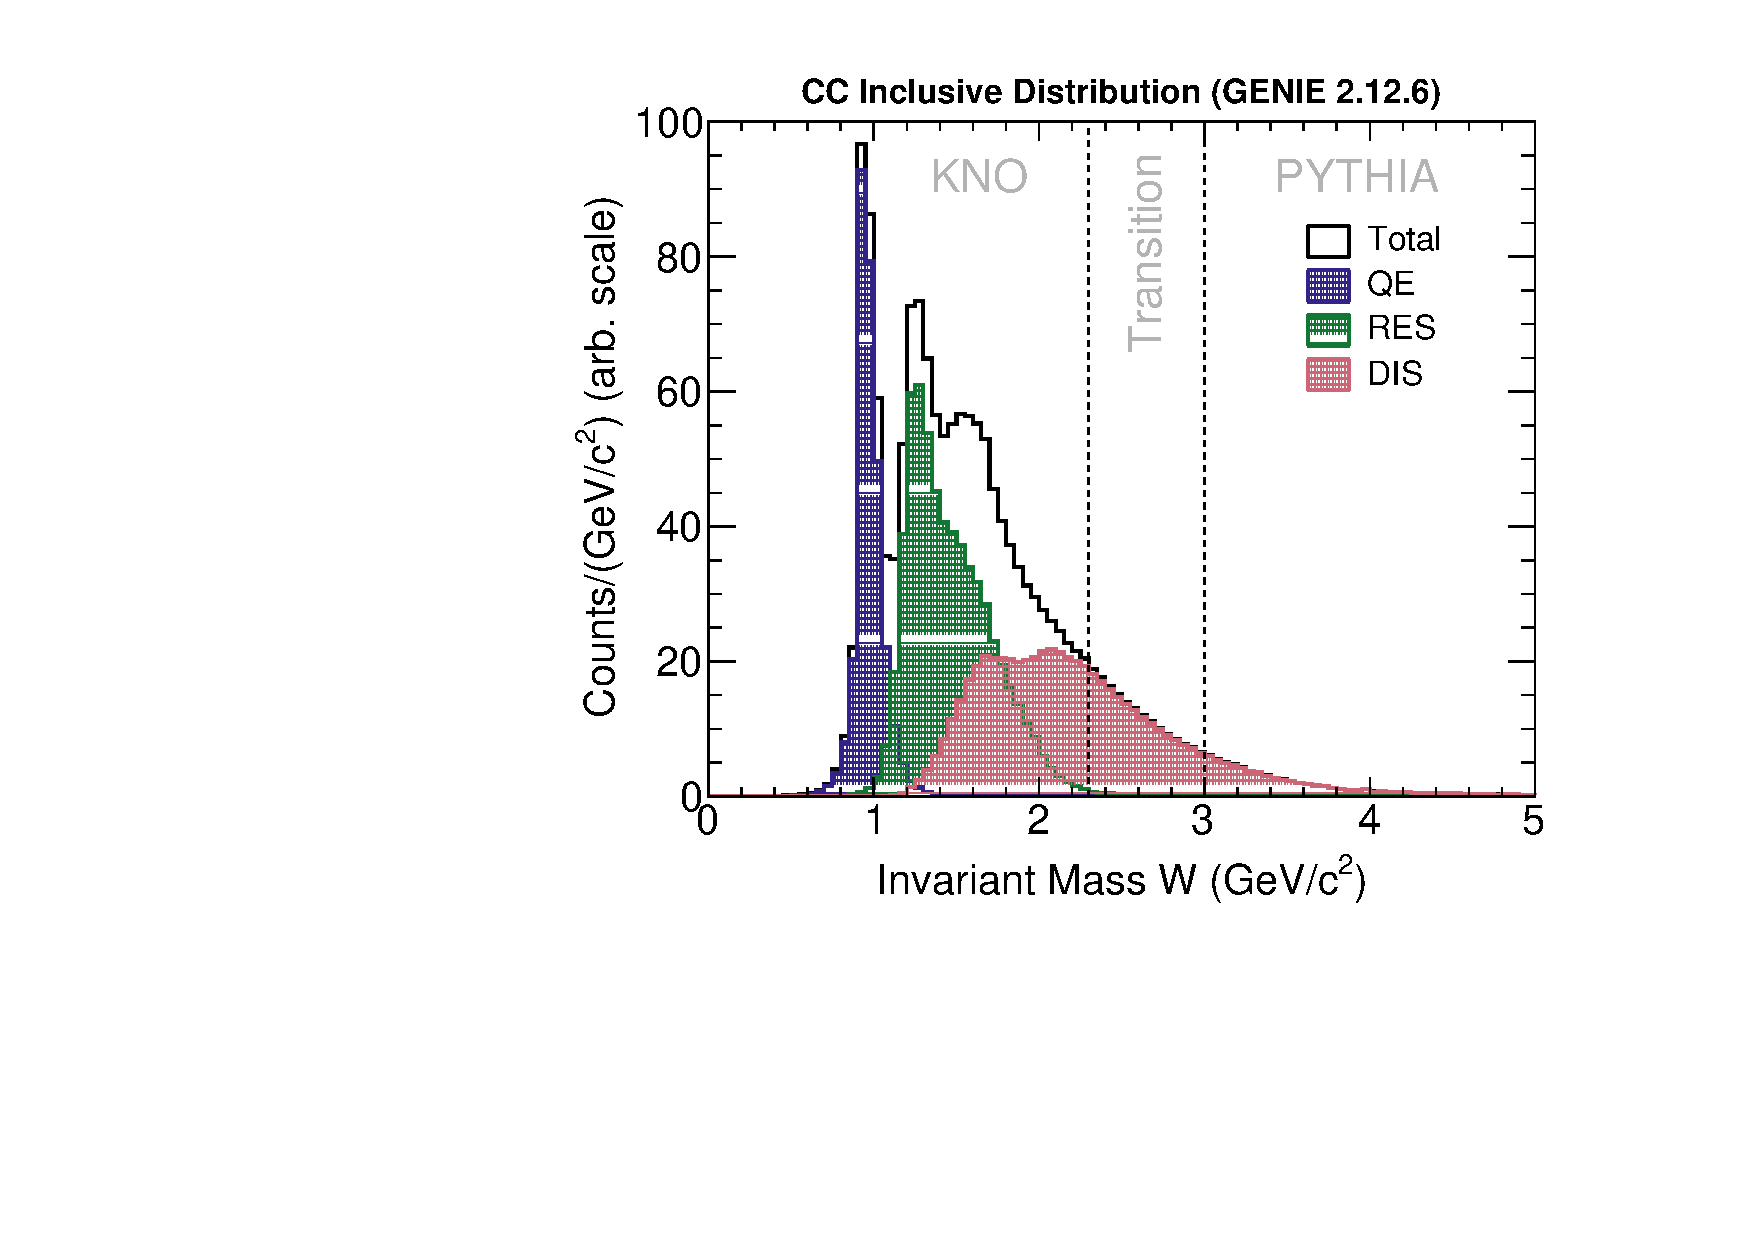
\includegraphics[width=0.8\textwidth]{05dataAsimulation/figures/WdistribGENIE.pdf}}%
  \caption{Invariant mass distribution $W$ of the charged-current antineutrino inclusive interactions on scintillator in GENIE 2.12.6, using the MINERvA antineutrino flux. The left blue region shows quasi-elastic scattering (QE), the middle green region represents resonance interactions (RES), and the right red region is deep inelastic scattering (DIS). The overlap between RES and DIS represents the transition region. The dashed lines split the $W$~distribution into the KNO-only region on the left, the PYTHIA-only region on the right, and the transition region in the middle. }
  %[short caption] {long caption}
  \label{fig:WdistribGENIE}
\end{figure}

% W distribution of ν µ-water target interaction in GENIE. For the flux, we use an atmospheric ν µ neutrino spectrum. Left red hatched region is quasi-elastic scattering, middle hatched region is resonance interactions, and right green hatched region is from DIS. The W distribution can be splitted to three regions, KNO scaling-baased model only region, PYTHIA only region, and the transtion region.

In contrast to the community definition of the DIS kinematic region of \mbox{$W >$ 2 GeV/$c^2$} and \mbox{$Q^2 >$ 1 (GeV/$c$)$^2$}, GENIE treats any non-resonant inelastic events as DIS. The antineutrino initially interacts with a single quark which then proceeds to hadronise, resulting in multiple hadrons in the final state. 

GENIE's DIS cross-section is calculated at the fully partonic level, accounting for the Bodek-Yang non-perturbative corrections to parton distribution functions (PDFs) as $Q^2$ decreases \cite{BodekYang_2003, BODEK2005113}, such as in the non-resonant pion production transition region described above. The Bodek-Yang model \cite{BodekYang_2003, BODEK2005113} also modifies the nuclear structure functions to incorporate nuclear effects as a function of Bjorken $x$, reflecting differences between nuclear and free nucleon structure functions, such as shadowing. Specifically, it utilises the parameterisations of charged lepton DIS measurements of $F_2^{\text{d}}/F_2^{\text{free}}$ and $F_2^{\text{Fe}}/F_2^{\text{d}}$, treating the axial and vector modifications equivalently. The same correction is applied to all nuclei.
%Bodek-Yang: https://arxiv.org/abs/hep-ex/0210024

%https://www.sciencedirect.com/science/article/pii/S0920563202017553
%Target mass correction is a kinematic correction where the mass of the target modifies the scattering kinematics and therefore the DIS structure functions. The higher twist correction is a dynamic correction due to non-perturbative parton-parton correlations. 

%https://arxiv.org/abs/0904.4043
The Andreopoulous-Gallagher-Kehayias-Yang (AGKY) model describes the hadronisation process in GENIE \cite{AGKY_Yang_2009}. In the AGKY model, the Koba-Nielsen-Olesen (KNO) model~\cite{KNO_KOBA1972317} is used for the \mbox{$W_{\text{min}} \leq $ 2.3 GeV/$c^2$} invariant mass, whereas the PYTHIA/JET\-SET~\cite{Pythia_Sjostrand_2001} program is utilised in the \mbox{$W_{\text{max}} > $ 3.0 GeV/$c^2$} region. The transition region $W_{\text{min}} < W \leq W_{\text{max}}$ is smooth as the fraction of PYTHIA hadronised events increases from 0\% to 100\% (and vice versa for KNO).

% AGKY: https://arxiv.org/abs/0904.4043
% KNO: https://www.sciencedirect.com/science/article/abs/pii/0550321372905512
% PYTHIA/JETSET: https://arxiv.org/abs/hep-ph/0010017

The KNO phenomenological model \cite{KNO_KOBA1972317} uses an empirical expression tuned to the Fermilab 15-foot bubble chamber neutrino-nucleon data to determine the hadron multiplicity \cite{AGKY_Yang_2009}. It selects particle content up to the multiplicity, generally a nucleon and any number of kinematically available low-mass mesons, e.g. $\pi$ and $K$. Finally, it partitions the available invariant mass $W$ among the generated hadrons to assign momenta. 

PYTHIA/JETSET \cite{Pythia_Sjostrand_2001} is a standard tool for the generation of high-energy collisions tuned to the BEBC data, spanning models for few-body hard processes to complex multihadronic final states. In the AGKY model, the PYTHIA region is not accessed until neutrino energy of approximately 3~GeV, and its contribution is equal to the one of KNO at around 9~GeV \cite{AGKY_Yang_2009}.
% Lund fragmentation function
% contains a library of hard pro- cesses and models for initial- and final-state parton showers, multiple parton-parton interactions, beam remnants, string fragmentation and particle decays.
% Tuned by NUX (MC generator for NOMAD)

%make figure like this 
%https://www.google.com/url?sa=i&url=https%3A%2F%2Fwww.researchgate.net%2Ffigure%2Fcolor-online-W-distribution-of-n-m-water-target-interaction-in-GENIE-For-the-flux-we_fig1_269635957&psig=AOvVaw3zlHm07k8xdJM4BFVcNKjs&ust=1700841191881000&source=images&cd=vfe&opi=89978449&ved=0CBIQjRxqFwoTCICvnqq92oIDFQAAAAAdAAAAABAE


\subsection{Final-state interactions}

Final-state interactions (FSI) occur as particles produced via the initial interaction traverse the nucleus to exit it. These interactions can change the final-state particle kinematics as well as the number of particles seen in the final state. GENIE models the FSI of nucleons and pions using intranuclear cascade simulation called INTRANUKE \cite{OGIntranuke_PhysRevD.45.743, RevisionIntranuke}. This analysis uses the effective data-driven model $hA$ \cite{genie_ANDREOPOULOS201087, genie_andreopoulos2015}. 

% OG intranuke: https://journals.aps.org/prd/abstract/10.1103/PhysRevD.45.743
% Revised intranuke: https://www.actaphys.uj.edu.pl/fulltext?series=Reg&vol=40&page=2445

The $hA$ implementation simulates the full cascade from a single effective interaction. It relies on the mean free path of the hadron to determine the probability that the FSI occurs. The interaction type, such as absorption, charge-exchange, elastic or inelastic scattering, relies on the external data, specifically cross-sections of ${\pi}^{+}$ and $p$ on \mbox{${}^{56}$Fe~\cite{genie_ANDREOPOULOS201087,genie_andreopoulos2015}}. Cross-sections are scaled by $A^{2/3}$ to predict FSI for other nuclei, and the isospin symmetry can be utilised to allow for predictions for $n$, $\pi^0$, and $\pi^-$. Furthermore, GENIE applies the FSI to the hadronic products of the interactions only, therefore the final-state muons are not affected.


%S. Dytman. INTRANUKE-hA. In AIP Conf Proc, volume 896, pages 178{184, 2007.
%https://arxiv.org/pdf/1510.05494.pdf

\begin{figure}[b!]
  \centering
  {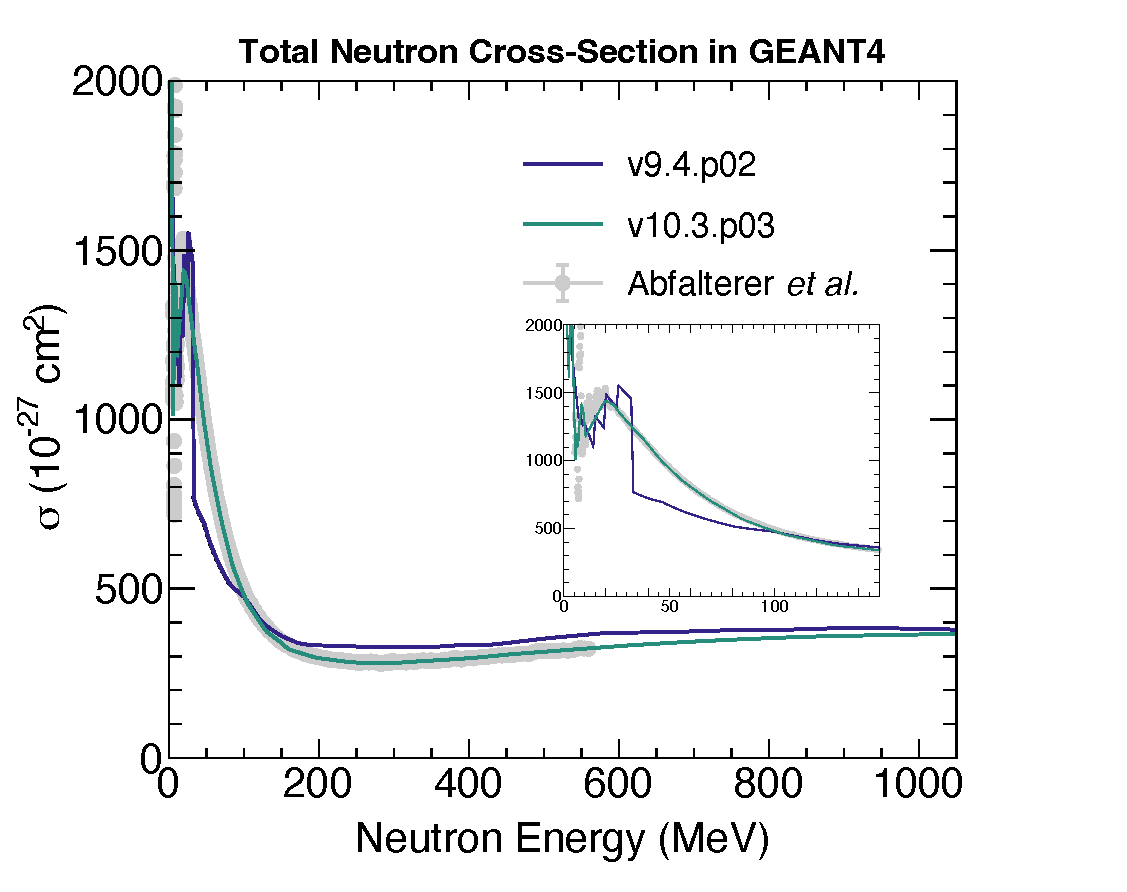
\includegraphics[width=0.8\textwidth]{05dataAsimulation/figures/totalNeutronXsec_wcloseup.pdf}}%
  \caption{Total neutron cross-section simulated by two different versions of GEANT4, v9.4.p02 and v10.3.p03, with overlayed Abfalterer \textit{et al.}~data~\cite{Abfalterer_PhysRevC.63.044608}. The older version of GEANT4 v9.4.p02 simulation shows significant disagreement with the Abfalterer \textit{et al.} data, whereas the newer version v10.3.p03 agrees with the data well. The insert shows the low neutron energy (0--200 MeV) behaviour of the two simulations versus data. }
  %[short caption] {long caption}
  \label{fig:neutronXsec}
\end{figure}

\section{Detector simulation}
Detector simulation models the propagation and the energy loss of the final-state particles through the MINERvA detector. Furthermore, it also accounts for the incidental activity in the detector via data overlay and employs the readout simulation to convert the energy deposits to simulated hits which can then be reconstructed.

\subsection{Particle propagation}
\label{sec:particleProp}

Particle propagation through the MINERvA detector uses the GEANT4 (GEometry ANd Tracking) software version 9.4.p02~\cite{Geant4_AGOSTINELLI2003250, Geant4_1610988}. The GEANT4 simulation proceeds in steps to determine if and how the final-state particles interact with a detailed description of MINERvA's geometry. The steps within a material are proposed by randomly sampling from the interaction length distributions implied by the interaction cross-sections for each process that applies to the particle. Based on the shortest step length, the particle either interacts or moves into a new material. Similarly, if an interaction produces secondary particles, their propagation is also simulated by GEANT4.

% Geant4: https://www.sciencedirect.com/science/article/pii/S0168900203013688
% Geant4: https://ieeexplore.ieee.org/document/1610988

The majority of interactions producing visible particles in the MINERvA detector come from the inelastic interactions. The inelastic hadron interactions in the detector use the QGSP\_BERT physics list, which employs the Bertini cascade (BERT) \cite{Bertini1963_PhysRev.131.1801,Guthrie:1968ue, Bertini1969_PhysRev.188.1711,BERTINI1971670} for particles with momentum less than \mbox{10 GeV/$c$} \cite{BertiniGeant4_heikkinen2003bertini}. For hadrons with momentum larger than \mbox{10 GeV/$c$}, GEANT4 uses the quark-gluon string precompound (QGSP) \cite{QGSP_folger2003string}. Other processes such as electromagnetic interactions or particle decays use the default modules of GEANT4. The particle propagation simulation ends with energy deposits and their associated timings along the track and at the end of the interaction step.

% Bertini cascade 1963: https://journals.aps.org/pr/abstract/10.1103/PhysRev.131.1801
% Bertini cascade 1968: https://www.sciencedirect.com/science/article/pii/0029554X68900542?via%3Dihub
% Bertini cascade 1969: https://journals.aps.org/pr/abstract/10.1103/PhysRev.188.1711
% Bertini cascade 1971: https://www.sciencedirect.com/science/article/pii/037594747190710X?via%3Dihub
% GEANT4 Bertini cascade: https://arxiv.org/abs/nucl-th/0306008v1
% QGSP in  GEANT4: https://arxiv.org/abs/nucl-th/0306007 

% Neutron is CV
% proton and pion just systematics
% neutron vs proton vs pion vs elastic
% reweight for neutron inelastic cross section
Furthermore, MINERvA reweights the events to modify the total neutron cross-section to match the Abfalterer \textit{et al.} \cite{Abfalterer_PhysRevC.63.044608} high-precision neutron scattering data which the newer versions of GEANT4 such as 10.3.p03 agree with \cite{Elkins2019_PhysRevD.100.052002}. The two GEANT4 total neutron cross-section simulations are compared to the Abfalterer \textit{et al.} data in Figure \ref{fig:neutronXsec}. The neutron interaction cross-section is increased via weighting up events with shorter tracks and weighting down events with longer tracks (and vice versa) while keeping the total number of (anti)neutrino events constant. A similar technique is used to evaluate the systematic uncertainties of the proton, pion and neutron interaction cross-sections and is further discussed in Chapter~\ref{ch:systematics}.


% MINERvA neutron reweight: https://journals.aps.org/prd/pdf/10.1103/PhysRevD.100.052002
% Abfalterer data: https://journals.aps.org/prc/abstract/10.1103/PhysRevC.63.044608

% MINERvA comparison Abfalterer vs Geant4: https://minerva-docdb.fnal.gov/cgi-bin/sso/RetrieveFile?docid=16284&filename=Kleykamp_2017-10-11_XsecNeutronOnX.pdf&version=3

% Systematics!! For example, for total inelastic cross-section for protons and pions, the variation is 10\% in carbon and hydrocarbon, 15\% in iron and 20\% in lead. Similarly, the neutron interaction cross-section is reweighted 
%https://minerva-docdb.fnal.gov/cgi-bin/sso/RetrieveFile?docid=7532&filename=dytman-hadr-uncert-27apr12.pdf&version=2


\subsection{Data overlay}
Additional effects such as particles produced in the rock between the NuMI beam and the detector, and overlapping (anti)neutrino interactions are not directly simulated. Instead, the MC hits are overlaid with data corresponding to random beam spills appropriate to the time periods in the simulation \cite{dataOverlay,TiceThesis2014}. The inserted data is flagged, ensuring it is not considered a signal candidate in the analysis.

% Internal MINERvA doc: https://minerva-docdb.fnal.gov/cgi-bin/sso/ShowDocument?docid=6032
% Tice thesis for data overlay/detector simulation: https://rucore.libraries.rutgers.edu/rutgers-lib/42462/

\subsection{Readout simulation}

Both the true deposits and timing need to be decalibrated to reconstruct the MC using the same methods as the data. First, all dead channels coming from the data overlay detector readout window are masked from the readout to account for the detector dead time and dead channels \cite{MarshallThesis2016}. 

% Marshall thesis dead channels: https://inspirehep.net/files/fd4468d48e6f7305f39526329836cf52
% Marshall internal detector simulation 101: https://minerva-docdb.fnal.gov/cgi-bin/sso/ShowDocument?docid=11234}

The energy deposited in the scintillator is converted into light yield using Birks' law \cite{Birks:1951boa}. The number of photoelectrons incident on the photomultiplier tube (PMT), which takes into account the attenuation of light in the fibres and additional smearing, is amplified using the gain of the PMT. The simulation also includes electronic noise and cross-talk. Finally, the photoelectrons are translated into raw ADC counts using the known analog-to-digital response \cite{WolcottThesis2015}.

% Wolcott thesis energy deposits to ADCs: https://www.osti.gov/biblio/1226351/

The simulated hit time is decalibrated by rounding to the nearest resolution width of the front-end-board (FEB) clock time. The known FEB offset and the travel time of photons to the PMT given the location of the hit along the scintillator strip is also added to the hit time and further smeared \cite{MarshallThesis2016}. 

% Marshall thesis time decalibration: https://inspirehep.net/files/fd4468d48e6f7305f39526329836cf52

% Birks law: https://iopscience.iop.org/article/10.1088/0370-1298/64/10/303
% Cross-talk



%the propagation and interaction or decay of the final state particles through the MINERvA detector.
 %This also includes simulating any secondary particles produces %from these interactions.

%This includes simulation o


%particle propagation
%data overlay
%readout simnulation
%mic track mathich efficiency weight
%particle  propagation weight





%- GENIE neutrino interaction simulation 
%- MINERvA interaction model reweighting
%- Detector simulation
%- simulation - reconstructed MC, truth
%- model 

\clearpage
\thispagestyle{empty}
\hfill
\clearpage
\chapter{Reconstruction}

\label{ch:Reconstruction}

Reconstruction involves converting energy deposits, or hits, along with their positions and timings—calibrated as described in Section~\ref{sec:calibration}—into physical quantities essential for the physics interpretation. Since the completion of its physics run, part of MINERvA's data preservation efforts \cite{dataPreservation_fine2020}, in which I have been involved, was to integrate reconstruction tools across various analyses and produce unified files containing both low- and high-level reconstructed objects used in all current and future analyses. Recently, the first iteration of these files, passing validation studies, has been produced and is used in this measurement.

This chapter focuses on the individual components of the common MINERvA reconstruction tool relevant for measuring nuclear dependence in antineutrino scattering. Therefore, in addition to the low-level grouping of hits in time and space, the reconstruction of the antimuon---specifically its track, direction, and momentum---is discussed. Furthermore, the reconstruction of the hadronic recoil system, i.e., energy in the detector not associated with the antimuon, needed for calculating Bjorken $x$ as defined in the previous chapter is also described. Finally, as the accurate placement of the interaction vertex is crucial for studying how antineutrinos interact with different materials, MINERvA's machine-learning technique for doing so is briefly reviewed. Note that both the data and the simulation sample are reconstructed this way.

% time slicing
% time and energy calibrated
% hit clustering

\section{Hit clustering by time and position}

Multiple antineutrino and other particle interactions could occur during one data-taking period, i.e.~a 16~$\mu$s gate, of the MINERvA detector. To distinguish each interaction in time, hits within each gate are initially clustered in 24~ns time windows, referred to as slices, if their total energy deposition surpasses the threshold of 10 photoelectrons. This threshold corresponds to 2/3 of the signal over a plane for a normally incident minimum ionizing particle, such as a rock muon. The time slice is then extended forward to incorporate additional hits until the threshold requirement is no longer met, resulting in variable-length time slice windows. All subsequent reconstruction steps are performed within these time slices.

[Include a figure of color-coded time slices here]

Thereafter, hits within a plane that are 'touching' each other are grouped into clusters of various sizes based on total energy deposits, categorized as low activity, trackable, heavy-ionizing, or superclusters. These clusters are then subjected to further reconstruction processes, involving track finding for the antimuon and summing all other hits for the recoil system. Clusters are corrected for cross-talk and are excluded from consideration after being used in the reconstruction process. Each cluster is utilised only once. 

[Include a figure illustrating the clusters]


\section{Antimuon information}
% useful: Amy's thesis: https://scholarworks.wm.edu/cgi/viewcontent.cgi?article=7271&context=etd
% Description: https://minerva-docdb.fnal.gov/cgi-bin/sso/RetrieveFile?docid=10017&filename=Minerva101-2015-Reconstruction.pdf&version=2

% Muon track reco
Any antineutrino interactions in the MINERvA detector can be identified by the produced antimuon. An (anti)muon, being a minimum ionising particle (MIP), leaves a distinctive signature of a long straight track in the detector. As described in Ref.~\cite{Aliaga_2014}, the reconstruction starts with finding trackable and heavy-ionising clusters forming a straight track in a minimum of three planes in each of the three views. Any additional clusters with slope and intercept consistent with this straight-track topology are added in each view.

The two-dimensional (2D) candidate tracks from each view are combined into a three-dimensional (3D) track if they are compatible to form a straight line. Due to the aforementioned three-plane requirement for the 2D candidates and the plane configuration of the MINERvA detector, as discussed in Section~reference[], the 3D track must span at least eleven planes in total. Subsequently, the track is fitted using Kalman filter [cite Kalman filter], considering the potential multiple scattering of the (anti)muon track. %It minimizes the local $\chi^2$ of the sum of the distance between the cluster position and the estimated track parameters, including track angle and position. The resulting straight track is projected upstream and downstream, including any clusters along this projection. 
Any super-cluster included in this way is subdivided into smaller clusters, ensuring the cluster energy aligns with that of a MIP---otherwise, they are removed and accounted for as a part of the recoil system. The fitted (anti)muon track has a resolution of 3~mm \cite{Aliaga_2014}.

% MINOS matching
For the antineutrino interaction to be considered in this work's measurement, the antimuon must have its charge (positive to be identified as antimuon) and its momentum measured by the MINOS spectrometer---various details and constraints of the MINERvA--MINOS combination are discussed in Chapter~\ref{sec:MINOS}. Therefore, the antimuon track found in the MINERvA detector must be matched to the one found in the MINOS spectrometer within a 200~ns time window. The tracks are matched if the difference between the end-point of MINERvA track projected upstream and the start of the MINOS spectrometer track (and vice versa) is less than 40~cm. The (anti)muon track reconstruction in the MINOS near detector has similar steps to the MINERvA reconstruction.

% Muon momentum recontruction
The antimuon momentum in the MINOS spectrometer is reconstructed either by range or curvature, utilising the magnetic field. Typically, (anti)muons with momenta up to 6~GeV/$c$ were contained within MINOS and were thus reconstructed by range, i.e.~total energy loss through interactions, with momentum resolution of 5\%\cite{Aliaga_2014, PhysRevD.81.072002}. In order to reconstruct (anti)muons originating from interactions in the MINERvA detector, they had to enter MINOS and penetrate at least 25.4~cm into it, requiring a minimum (anti)muon momentum of about 2~GeV/$c$ \cite{Aliaga_2014}. (Anti)muons with higher momenta were reconstructed by curvature with 10\% momentum resolution \cite{PhysRevD.81.072002}. Specifically, the antimuon momentum $p_{\text{MINOS}}$ measured in the MINOS spectrometer  by curvature is proportional to the magnetic field $B$ over the measured radius $R$ of the curvature, 
\begin{equation}
    \label{eq:momByCurvature}
    p_{\text{MINOS}} \text{ }[\text{MeV}/c] = \frac{0.3B\text{ }[\text{kGauss}]}{R\text{ }[\text{cm}]} \hspace{5pt}.
\end{equation}
% systematics MINOS
%The additional systematic uncertainties on muon momenta measured by curvature are 0.6\% for muons with momenta greater than 1 GeV/c and 2.5\% for those less than 1 GeV/c. The range and curvature uncertainties for muons measured by curvature are added in quadrature to obtain the total muon momentum uncertainty for muons measured by curvature of 2.1\% (3.1\%) for muons with momenta above (below) 1 GeV.
In addition to the antimuon momentum measured by MINOS, the total antimuon momentum also accounts for the energy loss while traversing the MINERvA detector, i.e. $p_{\text{total}} = p_{\text{MINOS}} + p_{\text{MINERvA}}$.

% systematics MINERvA
% The reconstructed energy loss in Minerva has two sources of uncertainty. The first source is the parameters of the Bethe Bloch equation, which varies the energy by 30 MeV for tracks that start in the active tracker region and 40 MeV for tracks that start in the nuclear target region. The second source is the material assay, which can vary the energy by 11 MeV for tracks that start in the active tracker region and 17 MeV for tracks that start in the nuclear target region.

The antimuon track reconstruction, i.e., determining the direction and momentum of the antimuon, is performed in the detector coordinates, which differ from the antineutrino beam coordinates as defined in Chapter~\ref{ch:minerva}. To express quantities with respect to the incoming antineutrino beam, the antimuon momentum vector in the detector coordinates is rotated 3.34$^{\circ}$ downwards in the $y$-$z$ plane to align with the beam coordinates. Subsequently, the transverse antimuon momentum $p_{\text{T}}$ is calculated using the rotated antimuon momentum vector, and it is, therefore, perpendicular to the beam direction, as illustrated in Figure~[make figure of the perpendicular pT].

%which is perpendicular to the beam direction is then reconstructed as
%\begin{equation}
%    \label{eq:pRotationX}
%    %\vspace{
%    p_x' = p_x, 
%\end{equation}
%\vspace{-38pt}
%\begin{equation}
%    \label{eq:pRotationY}
%    %\vspace{
%   p_y' = \cos (\theta_{\text{beam}}) p_y - \sin (\theta_{\text{beam}}) p_z,
%\end{equation}
%\vspace{-30pt}
%\begin{equation}
%    \label{eq:pRotationZ}
%   %\vspace{
%    p_z' = \sin (\theta_{\text{beam}}) p_y + \cos %(\theta_{\text{beam}}) p_z \hspace{5pt}.
%\end{equation}
%The transverse antimuon momentum $p_{\text{T}}$ which is perpendicular to the beam direction is then reconstructed as
%\begin{equation}
%    \label{eq:pTreco}
%    %\vspace{
%    p_\text{T} = \sqrt{p_x^2 + p_y'^2} \hspace{5pt}.
%\end{equation}

% NOTE
% beam direction facing 3.34 degrees downwards in the yz plane, hence rotation by 3.34 around x to get from the detector coordiante to the beam coordinates
% Rx(theta) = [ 1       0            0
%               0   cos(theta)   -sin(theta)
%               0   sin(theta)    cos(theta)  ]


\section{Recoil energy}
% calorimetric correction Anne Norrick: https://scholarworks.wm.edu/etd/1550153893/ (thesis)
% calorimetric correction Anne Norrick technote: 
% Devan: full detail %https://minerva-docdb.fnal.gov/cgi-bin/sso/RetrieveFile?docid=7712&filename=calorimetry-note.pdf&version=2
% depth mainly based on Amy
% https://scholarworks.wm.edu/etd/1681950288/


Any remaining clusters in the detector not associated with the antimuon track contribute to the hadronic recoil system, which is relevant for the calculation of Bjorken $x$ (excluding low-activity clusters identified as cross-talk). However, the recoil energy deposited by these clusters must be corrected to account for energy loss in the passive material of the detector. This process of estimating the energy of the hadronic recoil system is known as calorimetry. 

Specifically, the total energy of the non-antimuon clusters per subdetector is corrected by the sampling frequency\footnote{Sampling frequency is defined as the ratio of the energy deposited by an incident MIP in the active part of the detector divided by the sum of energies deposited by an incident MIP in the active and passive part.} of the given subdetector, also taking into account that the active scintillator planes are not fully active, as described in Chapter~\ref{ch:minerva}.\enlargethispage{2\baselineskip} The calorimetrically reconstructed recoil energy corrected for passive material overall is then the sum of these corrected subdetector energies. In the nuclear target region, the calorimetric correction is done cluster by cluster to account for the amount of passive material through which the resulting particles travel; for example, particles produced in target 1 traverse more passive material than those produced in target 5. In addition, if clusters are located only on one side of the target, the sampling frequency is calculated using half of the width of the passive target. A more detailed description of MINERvA's calorimetric correction can be found in Refs.~[cite]. 


%The calorimetrically reconstructed recoil energy corrected for passive material $E_{\text{recoil}}^{\text{reco, pmc}}$ is calculated as
%\begin{equation}
%    \label{eq:recoRecoil1}
%    %\vspace{
%    E_{\text{recoil}}^{\text{reco, pmc}} = \sum_{i}^{\text{subdetector}}\left( \frac{E_i}{f^{\text{sampling}}}\right) \times \text{scintillator active fraction}
%\end{equation}
%where the sum is performed over the individual subdetectors $i$ of the MINERvA detector and $E_i$ represents the total energy of the non-antimuon clusters in that subdetectors, and the $f_{i}$ term is the sampling frequency of the subdetector.  The expression also takes into account that the active scintillator planes are not fully active, as described in Chapter~\ref{ch:minerva}.

% f_sampling is (Eactive)/(Eactive+EAbsorber)
% sampling freqency page 11: https://cds.cern.ch/record/692252/files/ep-2003-075.pdf

% also binding energy of the struck nucleon within the nucleus
% or energy leakage out of the side of the detector.
Moreover, MINERvA also applies an additional calorimetric correction considering any differences between the above-corrected reconstructed recoil energy and the true recoil energy based on the true information available in the simulation, defined as the difference between the true antineutrino and true antimuon energy. This correction accounts for the loss of visible energy due to final state interactions (FSI), neutral particles, and other effects. Since these effects cannot be disentangled in an inclusive analysis, the correction is somewhat dependent on the underlying understanding of their behaviour encoded in the simulation. In this measurement, this is particularly relevant as antineutrino scattering produces final-state neutrons, whose kinetic energy cannot be reconstructed. Furthermore, this correction is energy dependent. Higher energy processes can have more significant FSI, produce more neutral particles in final states, etc. Therefore, it is applied bin-by-bin as a spline correction.~Historically, this correction process was carried out at the reconstruction level for each analysis separately. However, to support the new data preservation analysis files enabling all current and future analyses, I implemented this process on the post-reconstruction level within the high-level MINERvA Analysis Toolkit~(MAT) \cite{MAT_Messerly_2021}. This also allows for future improvements of these corrections using simulations with improved interaction models if necessary. 

In particular, this additional spline correction is calculated by the fractional 

applied as a multiplicative factor to the reconstructed recoil energy corrected for passive material. 



- true recoil energy directly from the simulation as the difference between the known antineutrino and antimuon energy
-  reconstruction more complex combining clusters not attached to antimuon in each materila, correcting them based on the fraction of the passive material in that region 
- passive matrial correction pont to Anne's thesis
- normalisation correction found by comparing true and the reconstructed sum
- correction to account for neutral particles such as neutrons by fitting  polyline the fractional difference between the calorimeric and true recoil energy such that the average difference is 0
- splines between 0 and 50 GeV

%This is calculated by looking at the fractional energy resolution of the calorimetric energy in bins of true recoil energy in the simulation. 


%A test beam program which used a scaled down version of the MINERvA detector in a charged particle beam was used to validate the calibration of the calorimetric response to single particles. It showed agreement between the data and simulation of particle interactions to within 4\% [72].


[ADD migration matrix with and without the correction]




%- calorimetric spline correction
%- passive material correction

\section{Interaction vertex}

%All events reconstructed using the machine-learning vertexing technique discussed in Chapter~{ch:Reconstruction} are by default so-called MINOS-matched events. This refers to interactions for which the antimuon track observed in the MINERvA detector was matched to the track observed in the MINOS spectrometer. The MINOS spectrometer is used to select positively charged muons, i.e. antimuons, based on the curvature of the track in the magnetic field. 



%\section{ML}


%https://minerva-docdb.fnal.gov/cgi-bin/sso/RetrieveFile?docid=16995&filename=MachineLearningVertexing.pdf&version=1



\chapter{Differential cross-section calculation}

\label{ch:analysis1D}
\vspace{-10pt}
This chapter delineates the specific steps I performed to extract the cross-section for MINERvA's first measurement of nuclear dependence in inclusive antineutrino scattering in medium energy. The analysis utilises data from an exposure of $1.12 \times 10^{21}$ protons on target (POT), and the simulation sample detailed in Chapter~\ref{ch:dataAsimulation}. Both the data and simulation were reconstructed using the techniques described in Chapter~\ref{ch:Reconstruction}. The differential cross-sections for carbon, hydrocarbon (scintillator), iron, and lead were determined using Equation~\ref{eq:xsec1D} for muon transverse momentum $p_{\text{T}}$ and Bjorken $x$. Additionally, the nuclear target to scintillator cross-section ratios were calculated using the matching flux technique discussed in Section~\ref{sec:nuclear_target_flux}. The results of this analysis are shown and discussed in Chapter~\ref{ch:results}, with the systematic uncertainties detailed in Chapter~\ref{ch:systematics}.

\iffalse
\fi
\section{Event selection}
\label{sec:eventSelection}

Event selection refers to a process of counting the number of interactions passing a set of selection cuts according to the analysis signal definition while taking into account the reconstruction capabilities of the detector. In this case, it ensures the cross-section is extracted for the charged-current interaction type inclusive sample of antineutrino scattering in a specific material. It is the first step of the cross-section extraction represented by $N_{\text{data}, j}$ in the Equation~\ref{eq:xsec1D} in Chapter~\ref{ch:measurement}.

The events considered in this analysis must meet the following criteria:
\begin{itemize}
    \item Charged-current antineutrino interaction producing an antimuon $\mu^{+}$
    \item Interaction occurring in a specific material, i.e. carbon, hydrocarbon iron, or lead
    \item Antimuon energy between 2 and 20 GeV
    \item Antimuon angle less than 17$^\circ$ with respect to the beam direction
\end{itemize}
The phase-space cuts included in the signal definition are determined by the detector's ability to reconstruct the antimuon, as discussed later.~It is also important to note that these selection criteria were also employed to compare the cross-section results with the corresponding samples from different (anti)neutrino event generators in Chapter~\ref{ch:results}.

Utilising the reconstructed data and the simulation sample from Chapter~\ref{ch:Reconstruction}, which comprises all MINERvA reconstructable MINOS-matched events, the same set of reconstruction cuts was applied to both samples. These cuts were aimed at identifying events that match the signal definition mentioned above, based on their reconstructed properties. Additionally, the reconstruction cuts serve to eliminate background events (i.e. non-signal events) and aid in the selection of events whose kinematics can be reconstructed while minimizing systematic uncertainties arising from the detector's reconstruction capabilities, as well as flux and interaction modelling. Most of these reconstruction cuts are shared across all MINERvA analyses as they stem from the MINERvA detector and the MINOS spectrometer designs. 

\begin{table}[b!]
    \centering

    \begin{tabular}{c c c c}
    \hline \\ [-1.5 ex]
    Target & Material & Number of events in data & Predicted purity (\%) \\ [0.5ex] % inserts table %heading
    \hline
    \hline
    2 & Iron & 75 786 & 84.4 \\
      & Lead & 68 559 & 86.4 \\
    \hline
    3 & Carbon & 56 760 & 81.7 \\
      & Iron & 36 647 & 84.0 \\
      & Lead & 22 809 & 87.0 \\
    \hline
    4 & Lead & 65 469 & 75.9 \\
    \hline
    5 & Iron & 52 247 & 78.7\\
      & Lead & 35 068 & 81.6 \\
    \hline
    Tracker & Scintillator & 1 823 367 & 98.9 \\
    \hline
    \end{tabular}

    \caption{Number of antineutrino data events reconstructed and selected in all relevant targets of different materials and the scintillator tracker of the MINERvA detector, and the predicted purity of the selection based on the simulation.}
    \label{table:selectedEvents}
\end{table}


Furthermore, although the final cross-section results are reported for various materials, most of the analysis steps treat individual targets of different materials separately. This separation is necessitated by the distinct efficiencies of the various target and material combinations discussed later on in Section~\ref{ch:efficiency}, which result from their positions in the detector. Therefore, this is also taken into account in the list of reconstruction cuts, which is as follows:
\begin{enumerate}
    \item The antimuon detected in the MINOS spectrometer must have a positive curvature to ensure an $\bar{\nu}_{\mu}$ interaction occurred, i.e. $(q/p) > 0$, where $q$ is the antimuon's charge and $p$ its momentum.
    \item The high-energy antimuon reconstructed by curvature in the MINOS spectrometer must have a curvature significance at least 5$\sigma$ to reduce the tails of the muon energy resolution spread \cite{Joel_HighMomMuons}, i.e. $(q/p)/\sigma_{q/p} \geq 5$, where $\sigma_{q/p}$ is the error on the curvature.
    % this  (q\p)/sigma (sigma is the error on q\p)
    \item The antimuon track must be contained within the fiducial volume of the MINOS spectrometer and cannot cross MINOS coil hole described in Chapter~\ref{ch:minerva}, i.e.~the event track must fall within the radial distance of \mbox{$210~\text{mm} < R_{\text{event}} < 2500~\text{mm}$ \cite{Joel_HighMomMuons, MINOS:1998kez}.}
    % https://minerva-docdb.fnal.gov/cgi-bin/sso/ShowDocument?docid=10154
    \item The interaction vertex must be within the fiducial volume of the MINERvA detector. This is bounded by a hexagon with an $850$ mm apothem in the $x$-$y$ plane, and for mixed targets, the vertex must be located more than $25~\text{mm}$ away from the boundary between the different materials \cite{Aliaga_2014}.
    \item The event must not contain any dead channels, i.e.~channels insensitive to new energy deposits, induced by previous interactions in the path projected upstream of the muon track. This is to avoid rock muons whose tracks are partially lost due to the dead time from being confused with fiducial events \cite{Aliaga_2014}.
    % https://www.sciencedirect.com/science/article/pii/S0168900214000035
    \item The event is excluded if the highest machine-learning probability for vertex placement falls below 20\% to eliminate instances where the network may be uncertain, maintaining a consistent and statistically significant contribution with similar pass rates for both data and simulation \cite{Klustova_MLsys}.
    % https://minerva-docdb.fnal.gov/cgi-bin/sso/ShowDocument?docid=29420
    \item For hydrocarbon (scintillator), the $z$ position of the machine-learning (ML) vertex must be in the tracker region, i.e. $5980~\text{cm} \geq z \geq 8422~\text{cm}$. For carbon, iron, and lead, the $z$ position of the interaction vertex must be located within the passive target 2, 3, 4, or 5 as described in Chapter~\ref{ch:Reconstruction}, and in the region of the $x$-$y$~plane corresponding to the respective material as discussed in Chapter~\ref{ch:minerva}. Target 1 is excluded from this analysis due to contamination from rock muons. As the most upstream target, it has only a small number of upstream tracking planes, making it challenging to distinguish an interaction in this target from a rock muon solely based on the antimuon track.
    % ML vertexing https://minerva-docdb.fnal.gov/cgi-bin/sso/ShowDocument?docid=16995
    \item The energy of the antimuon must be within the range of 2 to 20 GeV. The lower limit ensures that the antimuon possesses enough energy to traverse through the MINERvA detector and cross multiple planes in the MINOS spectrometer to form a track. Meanwhile, the upper limit serves to minimize neutrino contamination in the sample, particularly from unfocused high-energy mesons that have not undergone charge selection. Crucially, the 20 GeV cut-off is imposed due to an incomplete understanding of the flux modelling beyond this threshold.
    % cite Brian? 
    \item The angle of the antimuon with respect to the antineutrino beam must be less than~17$^\circ$.~This requirement is driven by the steep decline in the acceptance of the MINOS spectrometer for larger scattering angles, especially for interactions occurring in the most upstream nuclear targets. This is demonstrated in the $p_{\text{T}}$ efficiency plots, where $p_{\text{T}}$ serves as a direct proxy for the antimuon angle, later on in Section~\ref{ch:efficiency}.   
\end{enumerate}
Included in Appendix~\ref{ch:appendix_eventSelection} is an illustrative comparison showcasing the impact of each of these cuts on target 5 lead and the scintillator tracker in both data and simulation.

\iffalse
Target 5 Lead Data vs MC
MINOS matched events:
Antimuon:
5 sigma:
MINOS fiducial:
MINERvA fiducial:
Dead channels:
ML probability:
Tracker or Target + material:
Energy:
Angle:
\fi

The number of antineutrino events reconstructed and selected in all relevant targets of different materials and the scintillator tracker of the MINERvA detector is listed in Table~\ref{table:selectedEvents}.~In total, this measurement utilises an extensive dataset of antineutrino interactions: 56 760 in carbon, 164 680 in iron, \mbox{191 905} in lead, and 1 823 367 in hydrocarbon (scintillator tracker).~For comparison, this represents approximately $10\times$~more statistics than those in the MINERvA neutrino analysis in nuclear targets in low energy \cite{Tice_PhysRevLett.112.231801}, as mentioned in Section~\ref{ch:measurement}. Most importantly, it constitutes the largest sample of antineutrino interactions on various materials in the same beam ever analysed to date. 

\begin{figure}[t!] 
    \centering
    {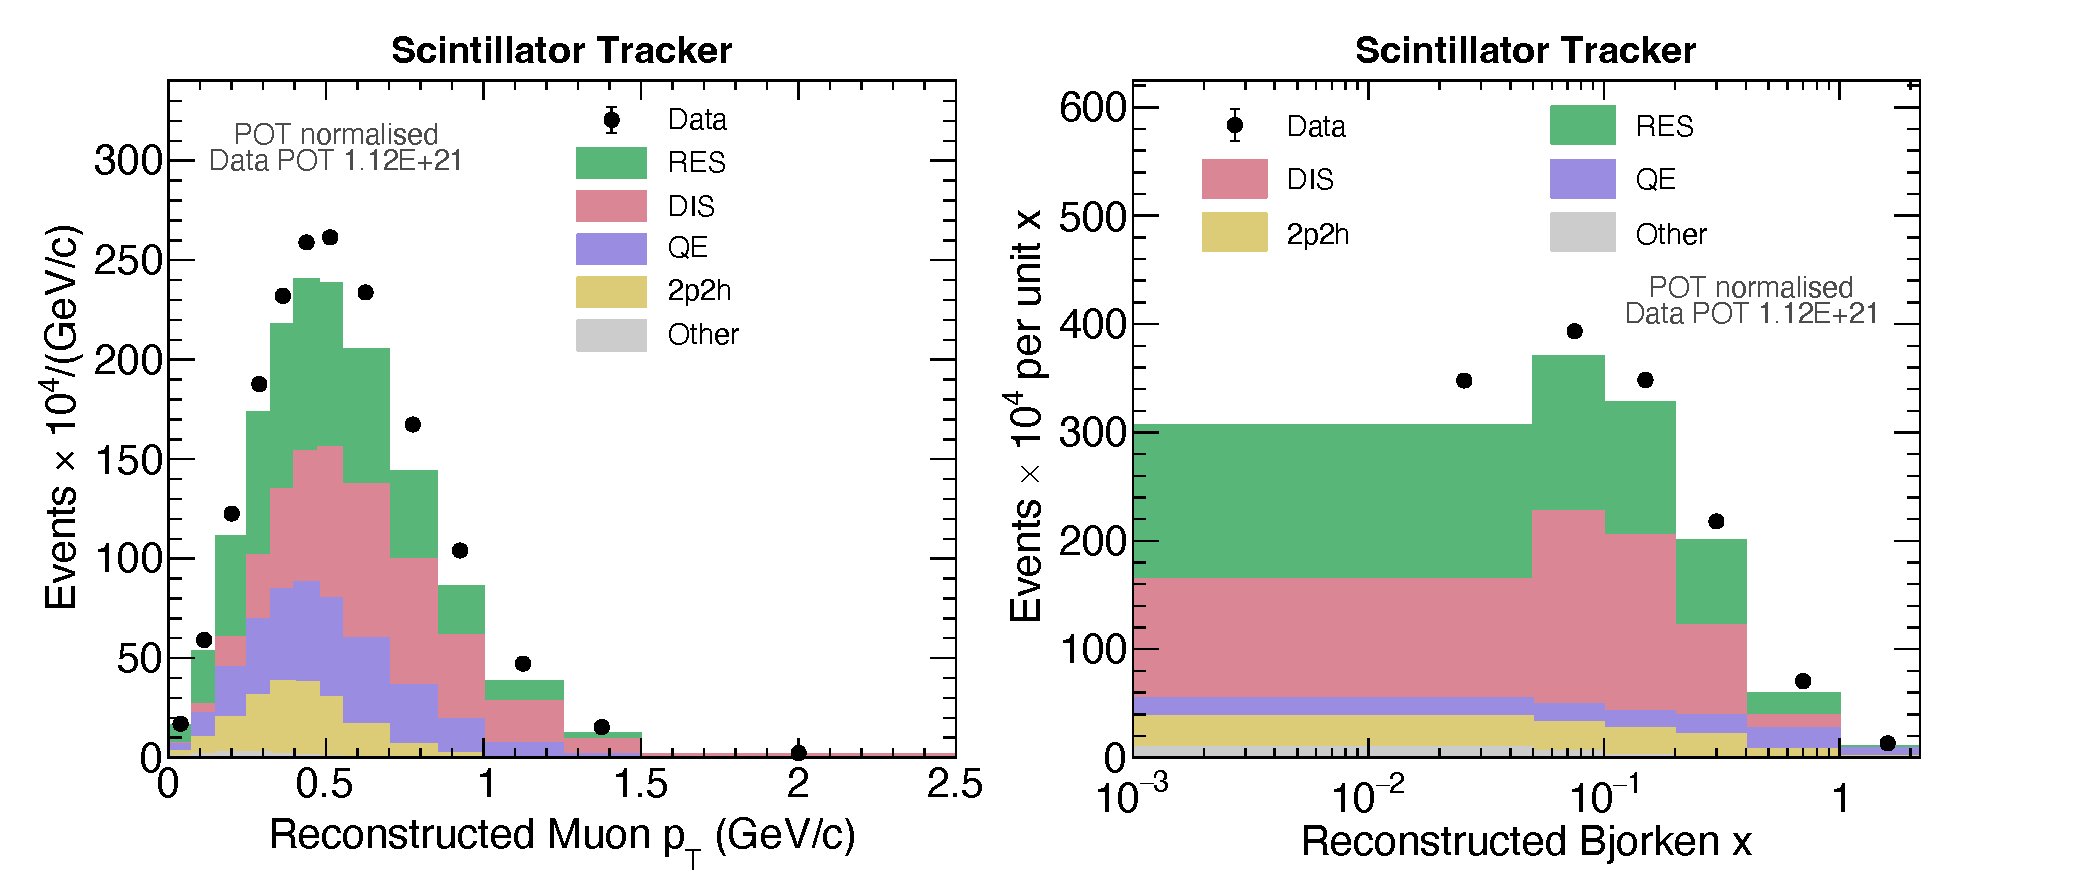
\includegraphics[width=1.\textwidth]{07analysis1D/figures/eventSelection_intType_tracker_pTx.pdf}}%
    \caption{Selected event distributions in the scintillator tracker for both antimuon $p_{\text{T}}$ (left) and Bjorken $x$ (right). The distributions are bin-width and POT normalised. The black points represent the data with its statistical uncertainty, while the simulation is broken down into the various interaction channels stacked in the descending order of their contribution:~resonant pion production (RES), deep inelastic scattering (DIS), quasi-elastic scattering (QE), 2p2h interaction (2p2h), and Other. The simulation visibly underpredicts the data in the scintillator tracker.}
    \label{fig:eventSelection_intType_tracker_pTx}
\end{figure}

Figure~\ref{fig:eventSelection_intType_tracker_pTx} displays the bin-width normalised distributions of selected events in the scintillator tracker for both variables of interest: muon $p_{\text{T}}$ and Bjorken $x$. Bin-width normalisation in this context means that each bin is divided by its own width. Therefore, the actual content of the bin is the number read off the $y$-axis (with $10^4$ included) multiplied by the bin width. The bin edges of antimuon $p_{\text{T}}$ and Bjorken $x$ are listed in Table~\ref{table:bindEdges}. The determination of bin edges involved optimizing the diagonal of a migration matrix explained in Section~\ref{sec:migration_unfolding}. This optimization aimed to retain the interesting $x > 1$ bin in the Bjorken $x$ distribution, as discussed in Chapter~\ref{ch:measurement}, while the lower bin boundary was approximately set using the definition of Bjorken $x$ in Chapter~\ref{ch:measurement} and the value of the lowest $p_{\text{T}}$ bin. Additionally, the $p_{\text{T}}$ distribution was truncated at 2.5 GeV/$c$ due to limitations of the MINOS acceptance, as demonstrated in the $p_{\text{T}}$ efficiency plots in Section~\ref{ch:efficiency}.

The simulation prediction for the scintillator tracker in Figure~\ref{fig:eventSelection_intType_tracker_pTx} is categorized by various interaction types. Given that this inclusive analysis utilises antineutrino data collected during the medium-energy (ME) physics runs of the MINERvA detector, where the antineutrino flux peaks near $6$ GeV, the predominant interaction types are resonant pion production and deep inelastic scattering.~Across all targets of various materials, resonant pion production contributes, on average, around 38\% to the sample, while deep inelastic scattering makes up about 32\%. Quasi-elastic scattering and 2p2h interaction constitute approximately 18\% and 11\% of the sample, respectively. Other interaction types, including coherent pion production and others, contribute less than 1\% combined. An example of the nuclear target 5 lead distribution with the simulation broken down into various interaction types is also included in Appendix~\ref{ch:appendix_eventSelection}.

\begin{table}[t!]
    \centering
    \small

    \begin{tabularx}{1\textwidth}{p{0.125\textwidth} p{0.028\textwidth} p{0.048\textwidth} p{0.038\textwidth} p{0.038\textwidth} p{0.046\textwidth} p{0.028\textwidth} p{0.046\textwidth} p{0.036\textwidth} p{0.028\textwidth} p{0.036\textwidth} p{0.026\textwidth} p{0.033\textwidth} p{0.026\textwidth} p{0.023\textwidth}}
    \hline \\ [-1.5 ex]
    Variable & \multicolumn{14}{c}{Bin edges} \\ [0.5ex] % inserts table %heading
    \hline
    \hline
    $p_{\text{T}}$ (GeV/$c$) & 0.0 & 0.075 & 0.15 & 0.25 & 0.325 & 0.4 & 0.475 & 0.55 & 0.7 & 0.85 & 1.0 & 1.25 & 1.5 & 2.5 \\
    \hline
    Bjorken $x$ & \multicolumn{2}{c}{0.001}  & \multicolumn{2}{c}{0.05}  & \multicolumn{2}{c}{0.1}  & \multicolumn{2}{c}{0.2}  & \multicolumn{2}{c}{0.4}  & \multicolumn{2}{c}{1.0}  & \multicolumn{2}{c}{2.2}  \\
    \hline
    \end{tabularx}
    \caption{Bin edges of the antimuon $p_{\text{T}}$ and Bjorken $x$ histograms used in this analysis.}
    \label{table:bindEdges}
\end{table}

The aforementioned reconstruction cuts may not exclusively isolate signal events, leading to a contamination of the data sample by background events—--interactions that exhibit a similar signature to signal events in the detector and are misidentified as such. To estimate the level of contamination in the reconstructed data sample, the simulation with known true information can be utilised. The metric that does that is called predicted purity, defined as
\begin{equation}
    \label{eq:purity}
    %\vspace{-10pt}
    \text{Purity} = \frac{\text{Signal events in the reconstructed sample}}{\text{All events in the reconstructed sample}} \hspace{5pt}.
\end{equation}
The analysis predicted purity for all relevant targets of different materials and the scintillator tracker of the MINERvA detector is listed in Table~\ref{table:selectedEvents}. The nuclear target purity averages around 82\%, while the scintillator tracker purity is almost 99\%. 
% target average: 82.4625

\begin{figure}
    \centering
    {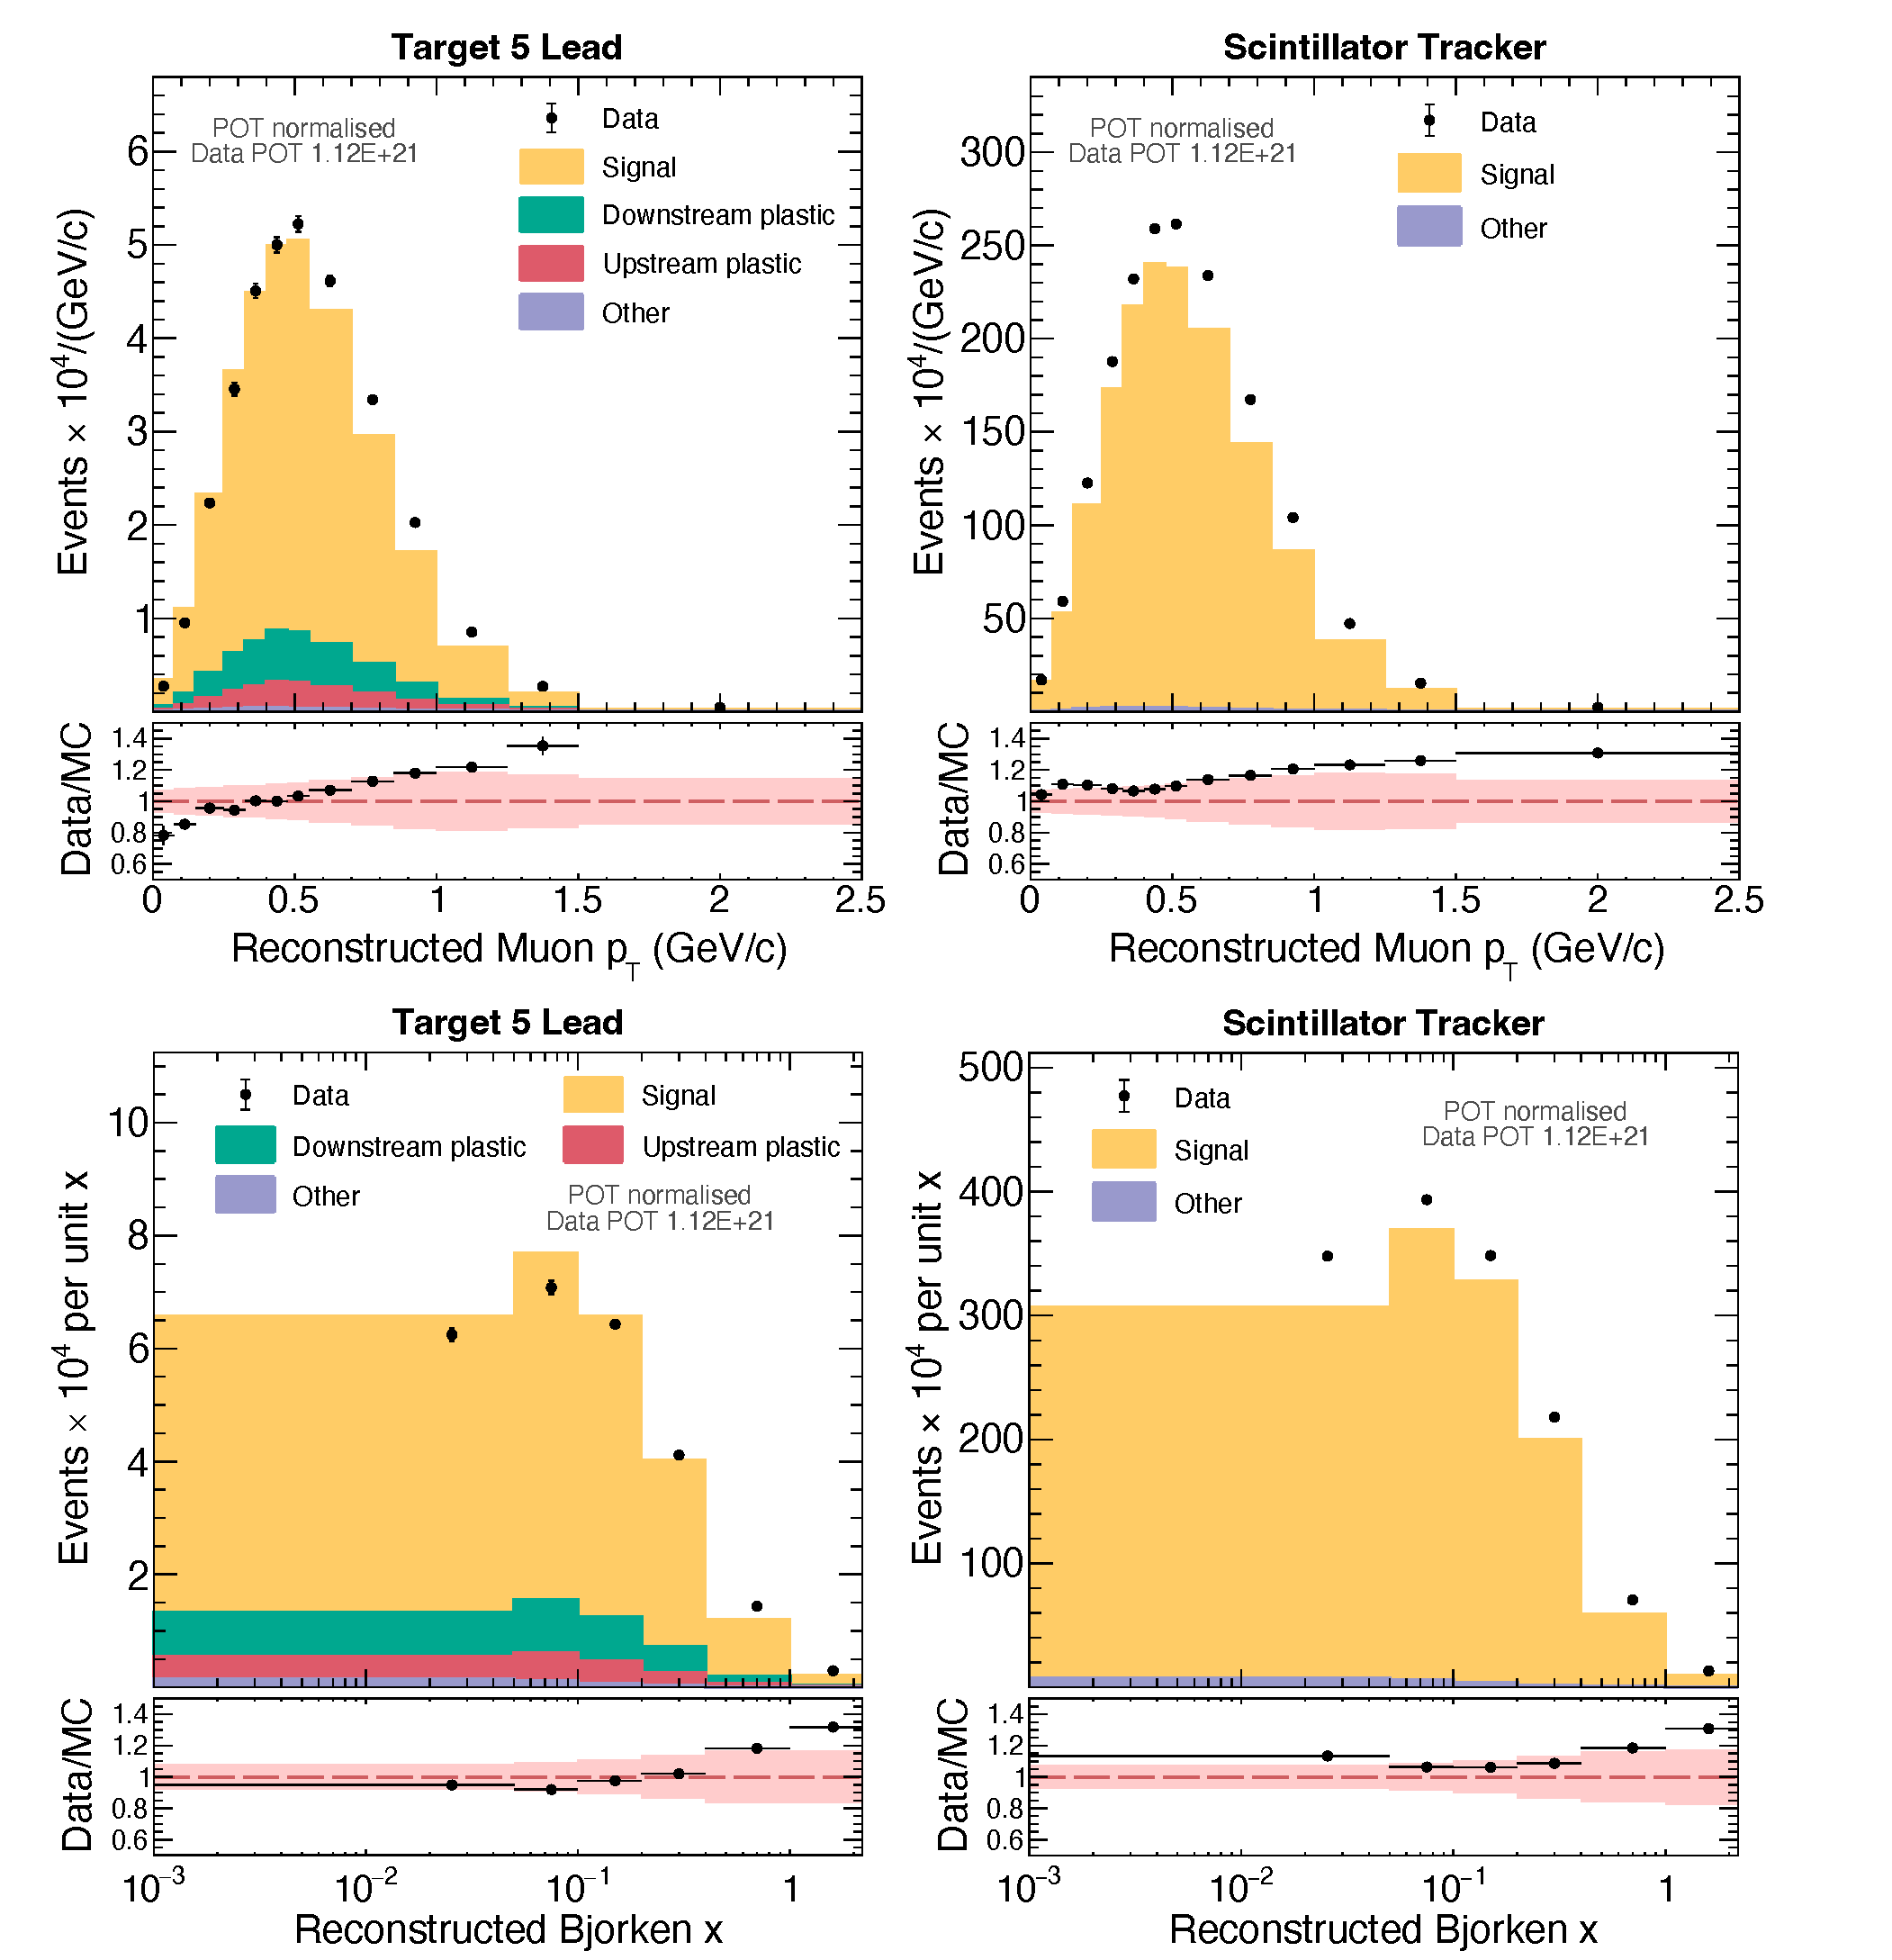
\includegraphics[width=1.\textwidth]{07analysis1D/figures/eventSelection_bkg_ratio_t5z82_tracker_pTx.pdf}}%
    \caption{Selected event distributions in target 5 lead (left panel) and the scintillator tracker (right panel) for both antimuon $p_{\text{T}}$ (top) and Bjorken $x$ (bottom). The distributions are bin-width and POT normalised. In the top panel of each plot, the black points represent the data with its statistical uncertainty, while the simulation is broken down into various sources of signal and background stacked in the descending order of their contribution. The bottom panel shows the data-to-simulation ratio. The solid band around the dashed line at 1 represents the systematic uncertainty on the simulation, while the black points carry the statistical uncertainty of the ratio. The horizontal lines on individual points indicate the bin width.}
    \label{fig:eventSelection_bkg_ratio_t5z82_tracker_pTx}
\end{figure}

Figure~\ref{fig:eventSelection_bkg_ratio_t5z82_tracker_pTx} illustrates a simulated breakdown of background in the reconstructed distribution for target 5 lead and the scintillator tracker, in both $p_{\text{T}}$ and Bjorken $x$. As depicted, the lower purity in targets, compared to the scintillator tracker, is a result of interactions reconstructed within the target that, in reality, occurred in the surrounding scintillator planes upstream (`Upstream plastic') and downstream (`Downstream plastic') of the relevant target. The `Other' category for targets combines events from different materials---for instance, in target 5 lead, it could include events from target 5 iron---and neutrino events contaminating the reconstructed charged-current antineutrino events. In the scintillator tracker, it combines the neutrino events with those from outside the tracker region instead. In both cases, it constitutes approximately 1\% of the reconstructed sample. The reconstruction cuts effectively eliminate any neutral current events. 

%Table~\ref{table:selectedEvents} also shows that the purity of nuclear target 4 and 5 is slightly lower than for the other targets. This is because they are thinner than the other nuclear targets as described in Chapter~\ref{ch:minerva}. Consequently, more events from the surrounding scintillator planes are prone to be misreconstructed in these thinner targets. 

It is also crucial to emphasize that there are no background events originating from outside the $x$--$y$ fiducial volume, the antimuon angle or the antimuon energy range depicted in Figure~\ref{fig:eventSelection_bkg_ratio_t5z82_tracker_pTx}. However, these backgrounds are appropriately accounted for in the final cross-section results through efficiency correction, allowing for their migration in and out of the sample during the unfolding procedure explained in Section~\ref{sec:migration_unfolding}. In practice, this involves applying the reconstruction cuts on the fiducial volume, energy, and angle range without utilizing the true information of the simulation for these aspects in the background subtraction, migration matrix, and efficiency numerator. The true information requirement is only included in the efficiency denominator.

Furthermore, the data-to-simulation ratio in Figure~\ref{fig:eventSelection_bkg_ratio_t5z82_tracker_pTx} serves as an initial indicator of how well the simulation predicts the data. While the simulation is tuned to encompass the latest measurements of neutrino pion production at MINERvA as described in Chapter~\ref{ch:dataAsimulation}, both the $p_{\text{T}}$ and Bjorken $x$ for target 5 lead and the scintillator tracker data distributions show a disagreement with the prediction, albeit in different ways.~All other selected event distributions with the background breakdown and the data-to-simulation ratios for the remaining nuclear targets of different materials are included in Appendix~\ref{ch:appendix_eventSelection}. 

The data distributions for the carbon-heavy scintillator tracker in both ${p_{\text{T}}}$ and Bjor\-ken~$x$ are generally higher than predicted by the simulation.~Nevertheless, the data mostly falls within the systematic uncertainties of the simulation prediction, except for the high ${p_{\text{T}}}$ and Bjorken $x$ region. The individual sources contributing to the systematic uncertainty band are discussed in Chapter~\ref{ch:systematics}. Similarly, the data distributions for target~3 carbon are also higher than the simulation prediction. The heavier iron targets show some agreement with the prediction at low ${p_{\text{T}}}$ and Bjorken $x$, but they are still underpredicted by the simulation at mid-to-high values of ${p_{\text{T}}}$ and Bjorken $x$. The data for the heavy lead targets exhibits a significant overprediction at low ${p_{\text{T}}}$ and Bjorken $x$, while still underpredicting the high ${p_{\text{T}}}$ and Bjorken $x$ region. In summary, the selected event distributions already indicate a significant nuclear dependence in antineutrino scattering which is not modelled by the simulation, especially in the low ${p_{\text{T}}}$ and Bjorken $x$ regions.

\begin{figure}[t!] 
    \centering
    {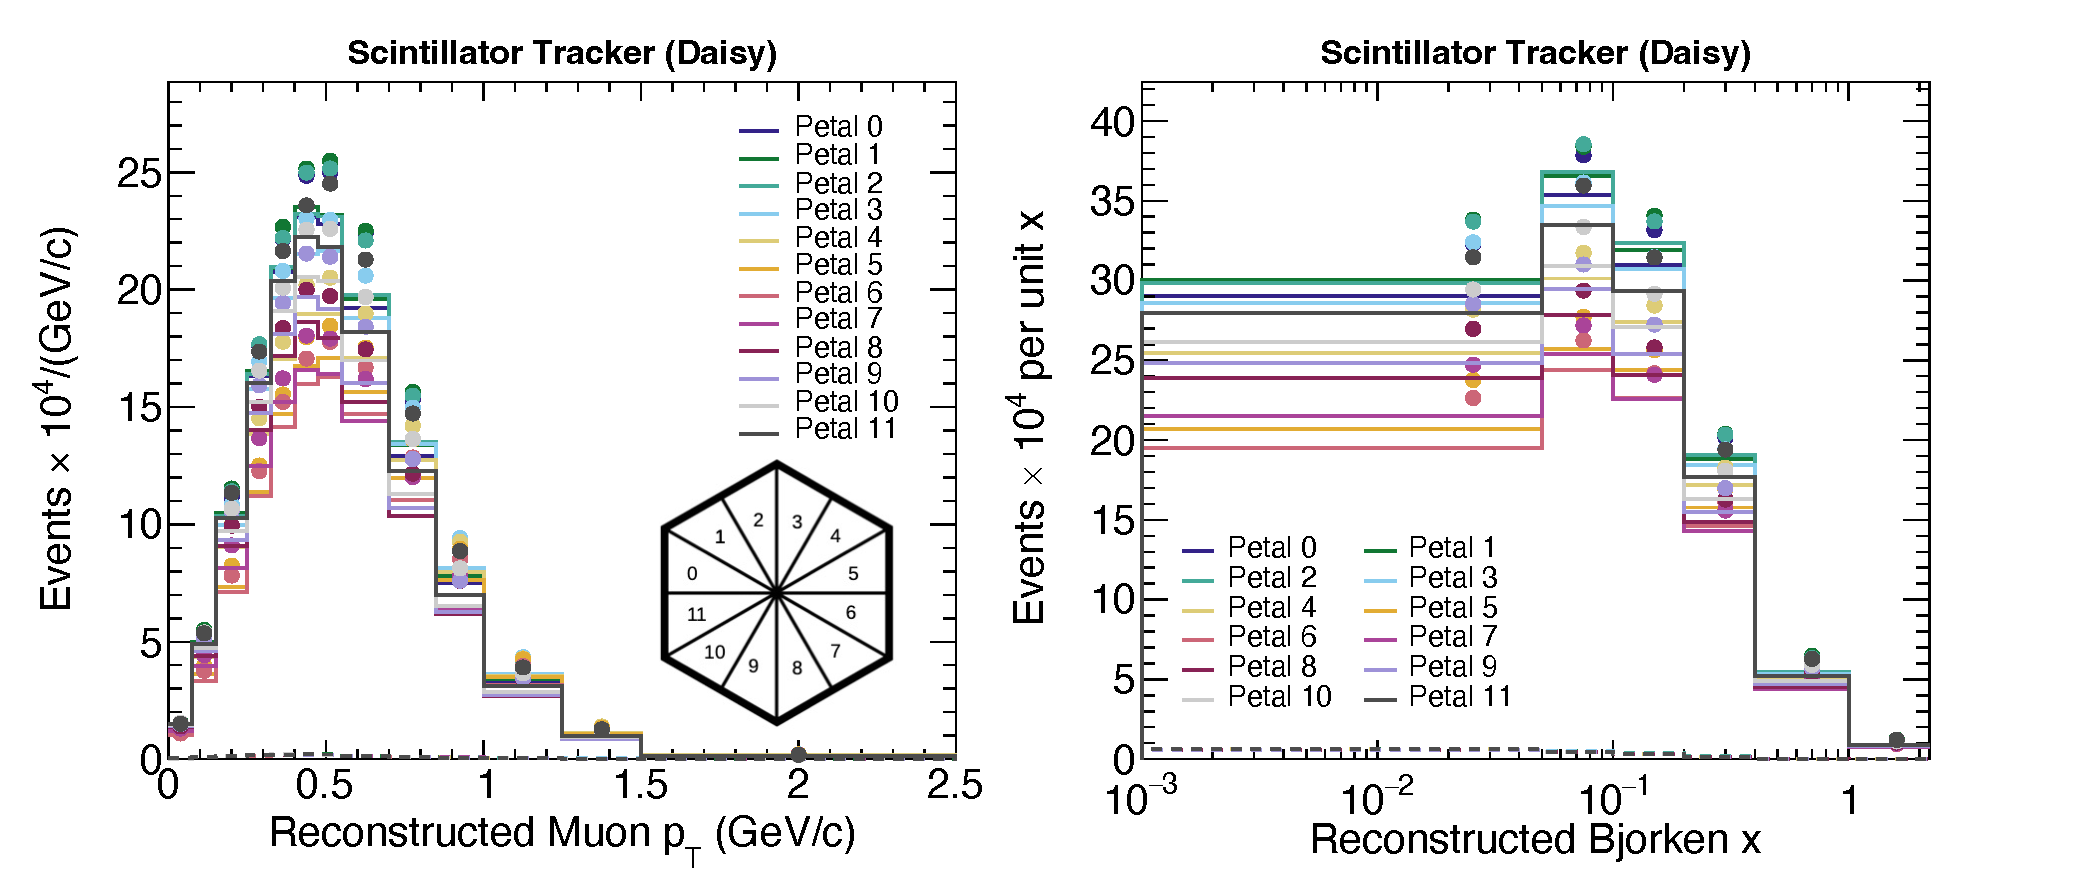
\includegraphics[width=1.\textwidth]{07analysis1D/figures/eventSelection_daisy_pTx.pdf}}%
    \caption{Selected event distribution for the scintillator tracker in `daisy petals' both in antimuon ${p_{\text{T}}}$ (left) and Bjorken $x$ (right). The simulation prediction for individual petals is depicted using coloured solid lines described in the legend, while the dashed lines show the simulated background prediction. For clarity, the uncertainty on the simulation is not shown. The corresponding points represent the data with its statistical uncertainty.~The hexagon insert illustrates petal positions looking downstream of the detector. }
    \label{fig:eventSelection_daisy_pTx}
\end{figure}

Finally, it is important to note that the scintillator tracker event distribution is also selected in 12 geometrical bins, referred to as ‘daisy petals’, as illustrated in Figure~\ref{fig:eventSelection_daisy_pTx} for both ${p_{\text{T}}}$ and Bjorken $x$. This extraction is essential for determining nuclear target-to-scintillator cross-section ratios using the matching flux technique discussed in Section~\ref{sec:nuclear_target_flux}. The number of events selected in each ‘daisy petal’ reflects the direction of the antineutrino beam traversing the detector. Additionally, ‘daisy petals' 5–7 experience a relative reduction in the number of events due to the MINOS coil cut.

\iffalse
Efficiency denominator - includes true angle cut and fiducial volume cut (x,y + separation). Angle and fiducial volume events are allowed to migrate in and out of the sample - efficiency corrected.
\fi
\newpage
\section{Background subtraction} \label{sec:bkgSubtraction}
% Here is a little trick because I am currently troubled with an issue 
% the cross-section for carbon when combine plastic sidebands and then 
% subtract vs use each plastic sideband separately and then combined background 
% subtracted stuff looks different
% Hence use: sidebands from the combined sidebands
% Background subtracted stuff from the seprate distributions so it's consistent... (somewhat lmao)
% Bkgs stuff from: /minerva/data/users/anezkak/10-25-2023_v430_p4/1D/combined/BackgroundSubtracted
% Sideband plots from: /minerva/data/users/anezkak/11-28-2023_v430_p4_combinedPlastic/1D/combined/PlasticSidebands


\newpage
\section{Migration and unfolding}
\label{sec:migration_unfolding}

\begin{figure}[b!] 
    \centering
    {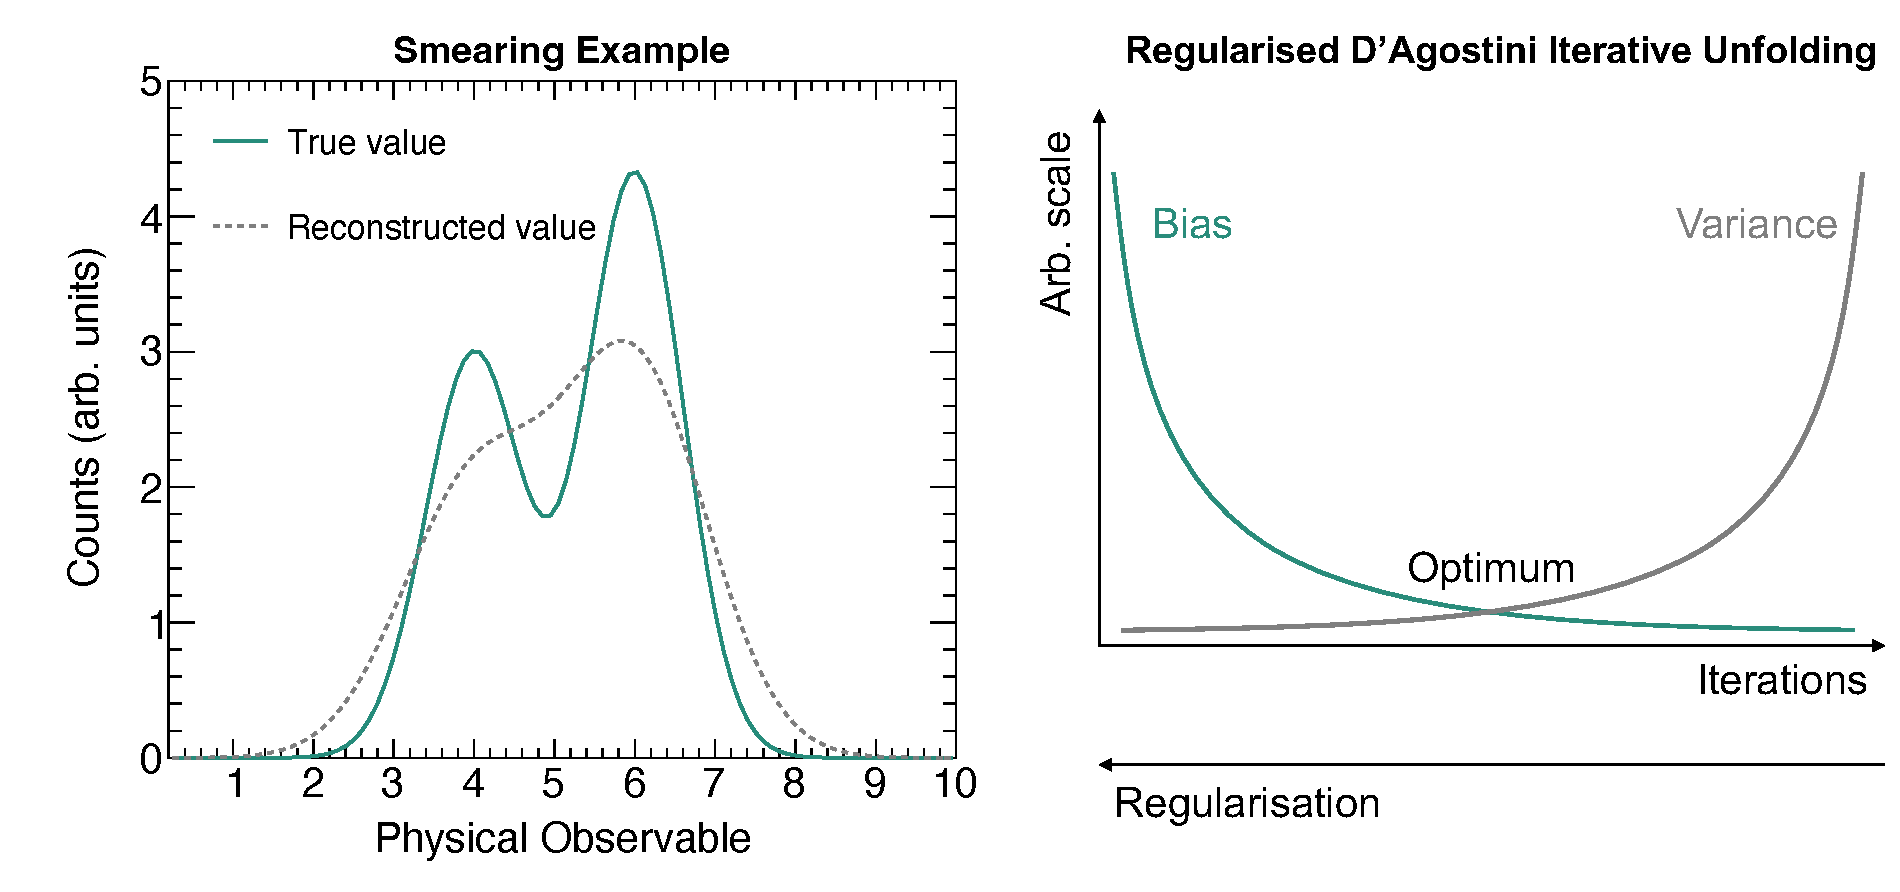
\includegraphics[width=1.\textwidth]{07analysis1D/figures/unfoldingExplanation_demo.pdf}}%
    \caption{Left: Smearing example of a two-component Gaussian model. The true histogram (solid line) shows more prominent peaks than the reconstructed histogram (dashed line) Right: Demonstration of the bias-variance trade-off in regularised D'Agostini iterative unfolding. Increasing the number of iterations leads to a less regularised solution with more variance. In practice, more variance also means that the statistical and systematic uncertainties increase rapidly. }
    % Intensities of the Poisson processes for the Gaussian mixture model data. Figure (a) shows the intensity function f of the true Poisson process and Figure (b) the intensity function h of the smeared Poisson process obtained by convolving the true intensity with a Gaussian of standard deviation σn = 1.2
    %[short caption] {long caption}
    \label{fig:unfolding_demo}
\end{figure}

Background-subtracted distributions offer the most accurate estimates of signal rates in reconstructed quantities. However, finite detector resolution and imperfect reconstruction may lead to deviations in the reconstructed kinematics of an event from its true kinematics, as demonstrated in Figure~\ref{fig:unfolding_demo}.~Put simply, there can be a difference between the actual physics that occurred and the physics that was measured. This effect, referred to as smearing, results in some events being reconstructed---or, in other words, migrated---into an adjacent or more distant bin than where they belong, smearing out the fine structure. The extent of this migration depends on how much lower or higher the reconstructed value is compared to the true value. The simulation sample, which contains both the true generated and the reconstructed information about the simulated events, is used to estimate the amount of smearing in data via a so-called migration matrix. 

%The migration matrix \textbf{$\text{K}^{\text{MC}}$} can be represented as a two-dimensional histogram relating the vector of bins of the true distribution $\boldsymbol{\lambda}$ on the $y$-axis and the vector of bins of the reconstructed distribution $\textbf{\text{n}}$ on the $x$-axis such as 
%\vspace{-10pt}
%\begin{equation}
%    \label{eq:smearing}
%    \vspace{-10pt}
%    n_{j} = \Sigma_{\alpha} K_{\alpha j}^\text{MC} %\lambda_{\alpha},
%\end{equation}
%using the known mapping.
The migration matrix can be represented as a two-dimensional histogram relating bin~$\alpha$ of the true generated distribution on the $y$-axis to bin $j$ of the reconstructed distribution on the $x$-axis, $U_{j\alpha}$. The more diagonal the matrix is, the less smeared the reconstructed distribution is. Examples of migration matrices for target~5 lead and the scintillator tracker in both $p_{\text{T}}$ and Bjorken $x$ are shown in the Figure~\ref{fig:migration_lead_tracker_pTx}. It is important to note that the migration matrices also consider underflow and overflow bins, which include values below or above the lowest and highest bin boundaries. This accounts for smearing in and out of the sample; however, these bins are not explicitly shown in Figure~\ref{fig:migration_lead_tracker_pTx}. All other migration matrices for passive targets and the scintillator tracker divided in the geometrical bins, i.e. `daisy petals', are included in Appendix~\ref{ch:appendix_migrationMatrices}.

\begin{figure}[b!] 
    \centering
    {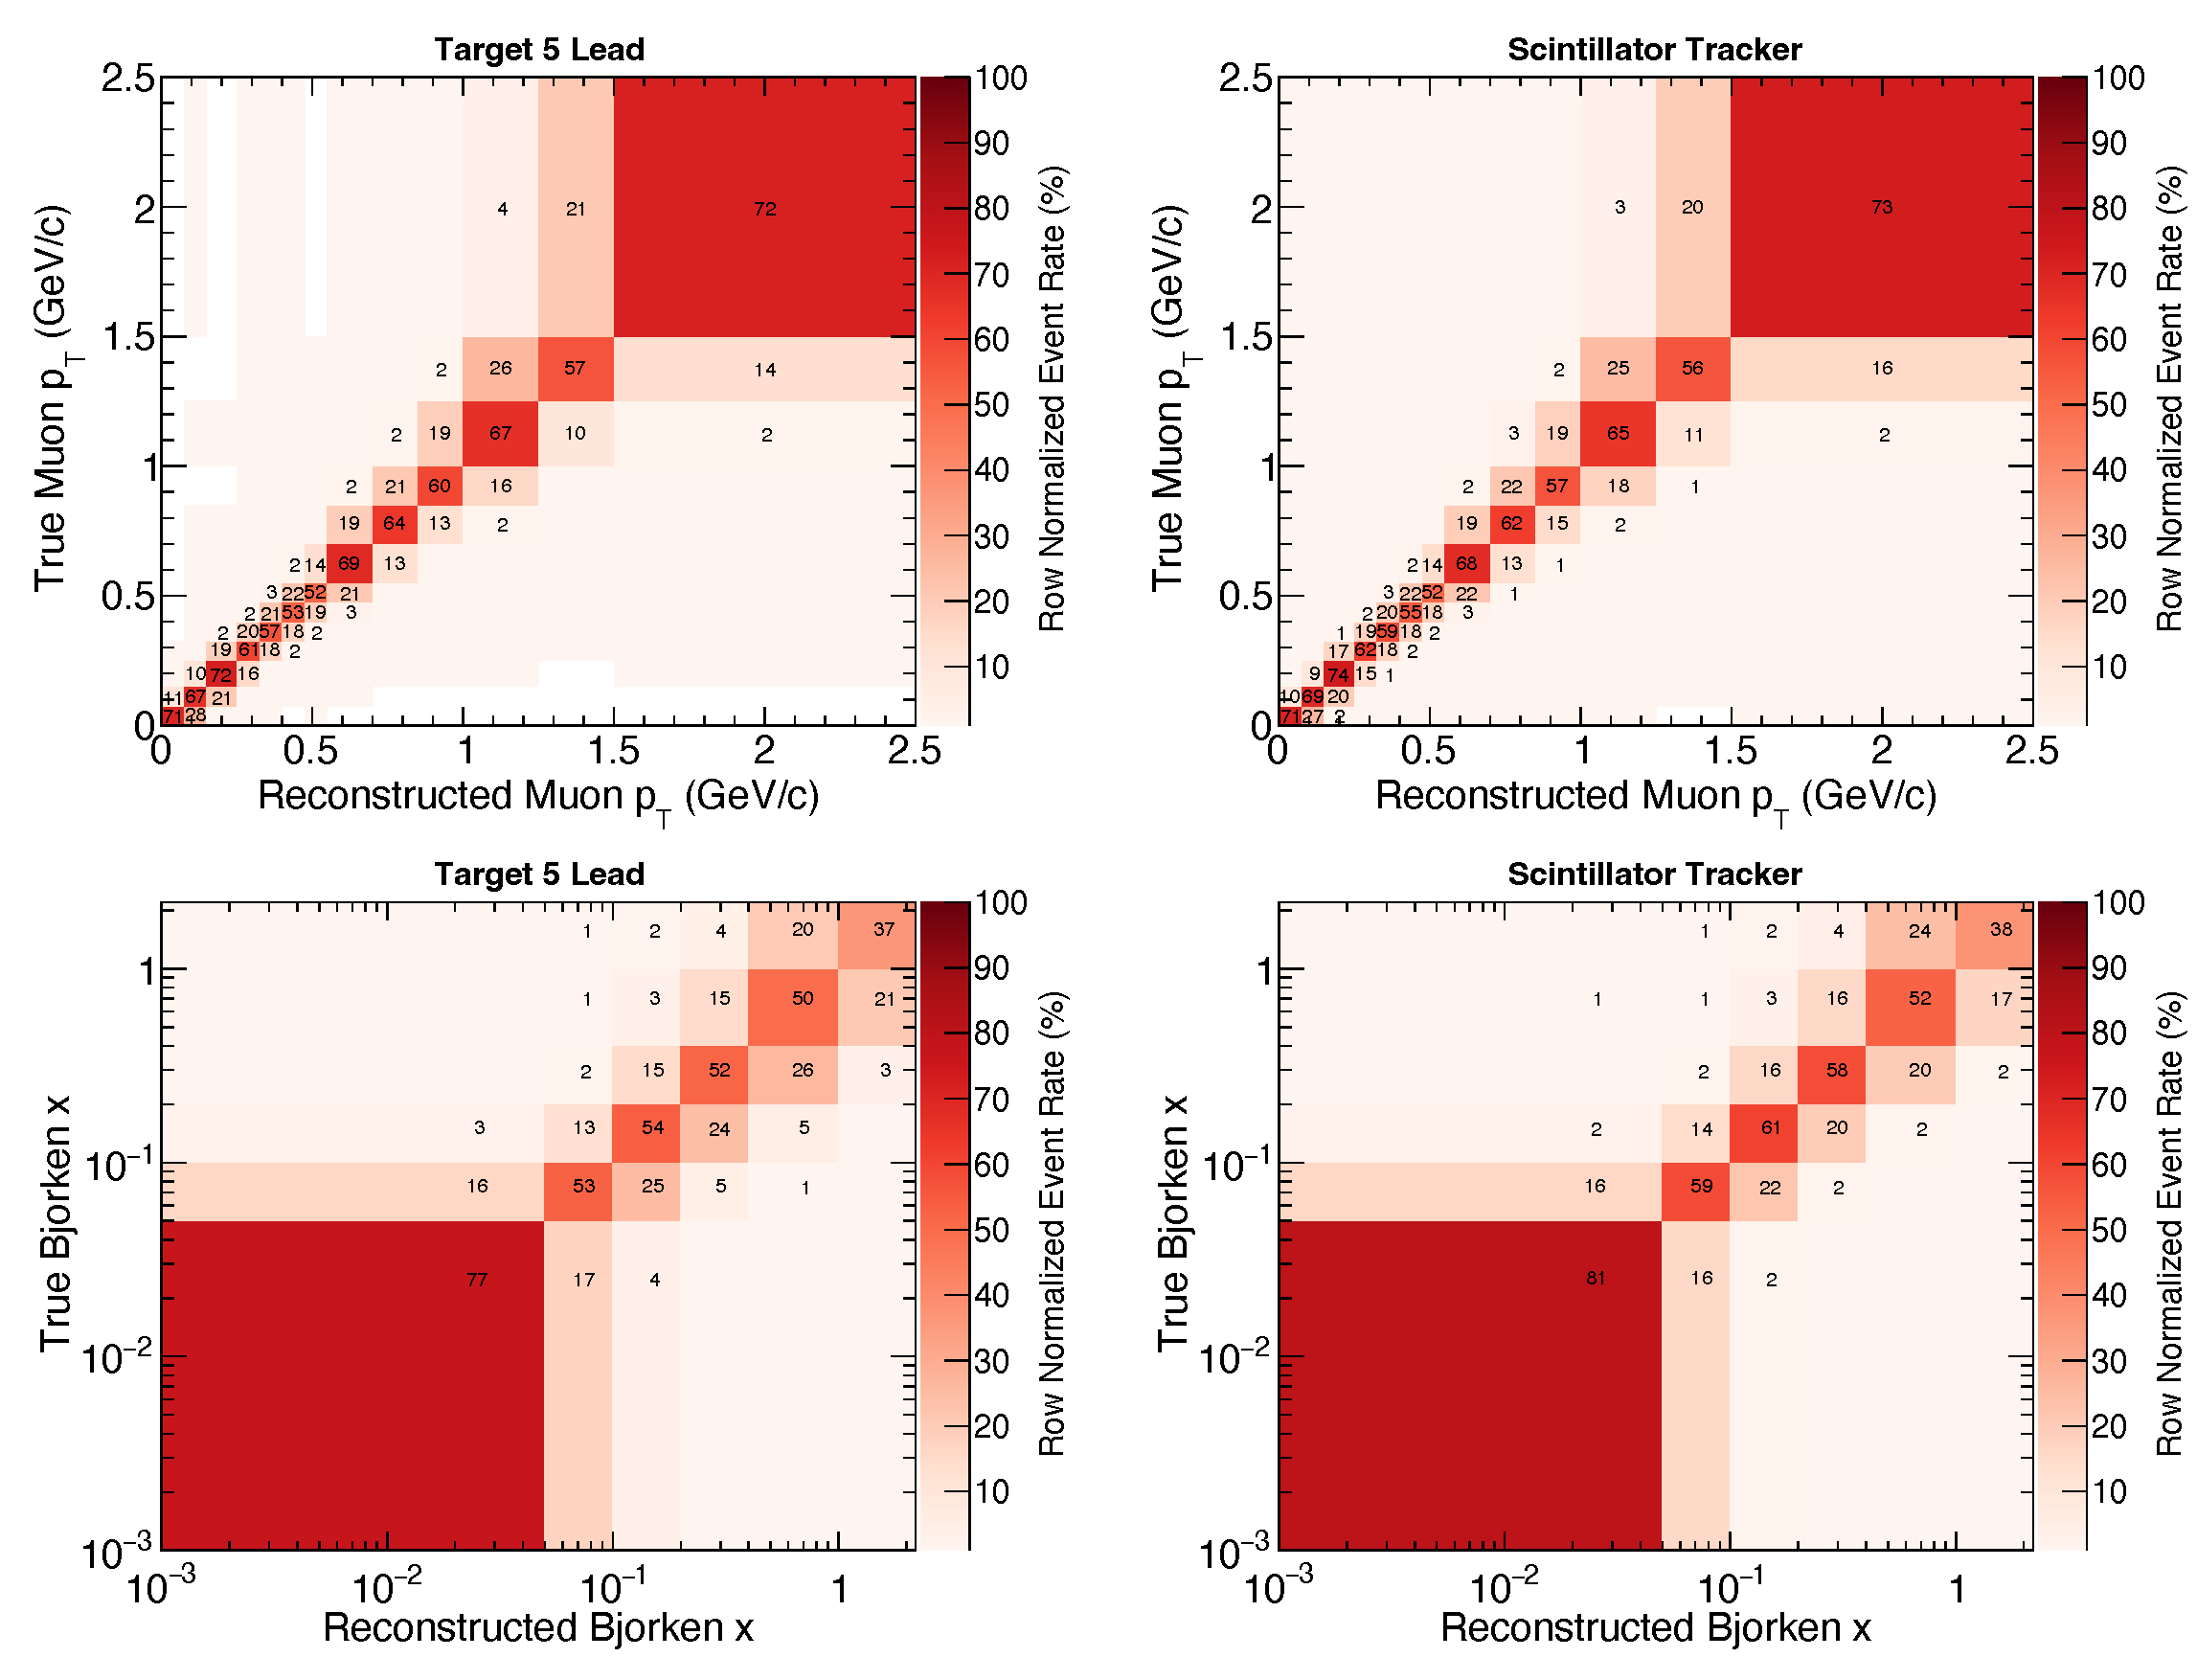
\includegraphics[width=1\textwidth]{07analysis1D/figures/migration_lead_tracker_pTx.pdf}}%
    \caption{Row-normalised migration matrices for target 5 lead (left panel) and scintillator tracker (right panel) both in $p_{\text{T}}$ (top) and Bjorken $x$ (bottom). Each row of the migration matrix is normalised to 1 to represent the probability that an event generated in a given bin $\alpha$ will be reconstructed in a bin $j$.}
    %[short caption] {long caption}
    \label{fig:migration_lead_tracker_pTx}
\end{figure}

The $p_{\text{T}}$ distribution is primarily smeared by the finite muon momentum resolution of the detector, stemming from the size of the scintillator strips affecting the length of particle tracks. On the other hand, the Bjorken $x$ distribution smearing likely arises from the calorimetric correction used to estimate the invisible energy from neutrons in the hadronic recoil energy reconstruction, as described in Chapter~\ref{ch:Reconstruction}. In addition, the region with $x > 1$, discussed in Chapter~\ref{ch:measurement}, is already inherently challenging at the true simulation level.~Events in this region predominantly originate from intranuclear scattering, and may not necessarily include other physics contributions such as short-range correlations indicated by electron-scattering data~\cite{CLAS:PhysRevLett.96.082501,SRC:annurev}. Therefore, caution is exercised when working with this particular bin. In general, the migration matrices are more diagonal in the scintillator tracker than in the passive target region due to better tracking (more active material). 


%and relying on the simulation to estimate the smearing effects in the data.
% needs a reference for electron-scattering
% My x > 1 region studies:
% https://minerva-docdb.fnal.gov/cgi-bin/sso/RetrieveFile?docid=29951&filename=collabMeeting_December2021.pdf&version=1
% https://minerva-docdb.fnal.gov/cgi-bin/sso/RetrieveFile?docid=29808&filename=October-2021_update_inclusives.pdf&version=1
% annual review

In order to report a detector-independent cross-section, the smearing of the reconstructed distribution must be reversed. The process of estimating the true distribution from the measured smeared spectrum is called unfolding. Unfolding the distributions is crucial for future reinterpretations of the result, combinations with other experiments, and aiding the understanding of various physics models. In the cross-section extraction Equation~\ref{eq:xsec1D}, the unfolding process is denoted by $\Sigma_{j} \tilde{U}_{j\alpha}$ acting on bin $j$ of the background subtracted reconstructed distribution.

% UNFOLDING IS AN ILL POSED PROBLEM
% Cowan, G. Statistical Data Analysis (Oxford University Press Distribution Services North Kettering Business Park Hipwell Road Kettering Northants NN14 1UA, 1998).
% https://indico.cern.ch/event/107747/contributions/32645/attachments/24317/35000/blobel.pdf
\begin{comment}
\begin{figure}[b!] 
    \centering
    {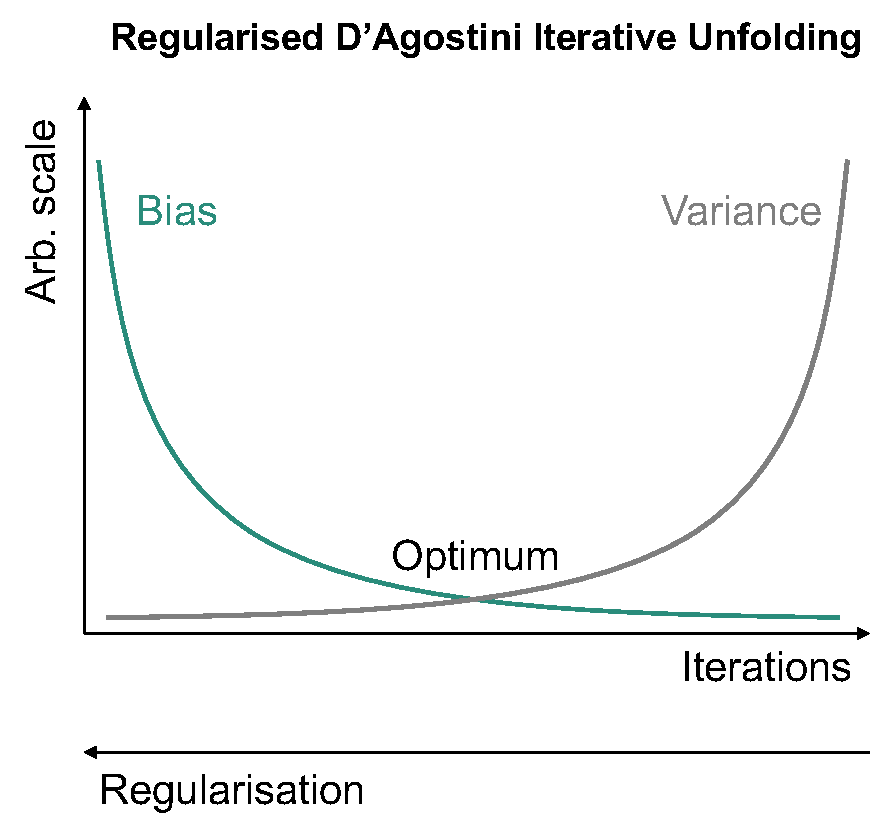
\includegraphics[width=0.8\textwidth]{07analysis1D/figures/unfoldingExplanation.pdf}}%
    \caption{Demonstration of the bias-variance trade-off in regularised D'Agostini iterative unfolding. Increasing the number of iterations leads to a less regularised solution with more variance. In practice, more variance also means that the statistical and systematic uncertainties increase rapidly. }
    %[short caption] {long caption}
    \label{fig:unfolding_explanation}
\end{figure}
\end{comment}

Unfolding could be achieved by inverting the migration matrix, which is, however, not always invertible. Moreover, unfolding is, by definition, an ill-posed problem as small changes in the measured distribution can lead to significant fluctuations in the true distribution, i.e.~large variance \cite{blobel2002unfolding}. Introducing regularisation in the unfolding process can address this issue by trading off some variance for a controlled amount of bias\footnote{Bias is defined as the difference between the expected value of the unfolded result and the true unmeasured expected value, which in the simulation is the true generated value.}. Similar to other MINERvA results, this analysis uses the D'Agostini iterative regularisation method~\cite{DAgostini:1994fjx,DAgostini:2010hil} implemented in the RooUnfold package~\cite{Adye:2011gm} in ROOT~\cite{ROOT_Brun:1997pa}, where the regularisation parameter is the number of iterations, as illustrated in Figure~\ref{fig:unfolding_demo}.
% Kevin McFarland:
%https://minerva-docdb.fnal.gov/cgi-bin/sso/RetrieveFile?docid=15224&filename=Unfolding%20MINERvA.pdf&version=2
% Kuusela unfolding
% https://infoscience.epfl.ch/record/220015?ln=en

%Uy=lambda
% lambda is truth
% y is measured data
% U is the migration matrix
% simulation-truth dependent. unfolding matrix is iteratively improved and applied to the data to give and improved estimate
The $(k+1)$th iteration of the D'Agostini method is determined by 
\vspace{-10pt}
\begin{equation}
    \label{eq:unfolding}
    \vspace{10pt}
    \lambda_{\alpha}^{(k+1)} = \frac{\lambda_{\alpha}^{(k)}}{\sum_{j=1}^N U_{j\alpha}} \mathlarger{\sum}_{j=1}^N \frac{U_{j\alpha}y_j}{\sum_{\beta=1}^P U_{j\beta}\lambda_{\beta}^{(k)}},
\end{equation}
where $U_{j\alpha}$ is the simulation-based migration matrix, $\lambda_{\alpha}^{(k)}$ represents the vector of bins of the true distribution at iteration $k$, and $y_{j}$ is the vector of bins of the reconstructed distribution.~In RooUnfold, the initial prior $\boldsymbol{\lambda}^{(0)}$ is the simulation prediction of the true distribution, i.e. $\boldsymbol{\lambda}^{(0)}$ = $\boldsymbol{\lambda}^{\text{MC}}$~\cite{Adye:2011gm}.~A more detailed description of the method can be found in the Appendix~\ref{ch:appendix_unfolding}.

In practice, the unfolding procedure is independently applied to both the central value histogram and all systematic universes. Since any statistical variation in the reconstructed distribution can be interpreted as a smearing of the fine structure of the true distribution, unfolding the distribution using many iterations results in the statistical and systematic uncertainties increasing rapidly. Therefore, it is crucial to determine the optimal number of iterations demonstrated in Figure~\ref{fig:unfolding_demo}, balancing the aforementioned reduction of bias while keeping variance minimal.~MINERvA analyses find this number of iterations via so-called warping studies.

Unfolding the underlying simulation with the migration matrix based on that simulation would result in perfect unfolding in one iteration, leading to maximum modelling bias. Therefore, warping studies involve the unfolding of fake data, referred to as `warped models'. These warped models are simulations that have been reweighted to depict alternative physics models, exaggerate features of the underlying distributions, or capture differences in the shapes of distributions between the data and the original underlying simulation. The reconstructed distributions of warped models, where the truth is known, are unfolded using a migration matrix based on the original underlying simulation. The number of iterations is then determined by looking at the least number of iterations required for $\chi^2$, defined as 
%\vspace{-10pt}
\begin{equation}
    \label{eq:unfolding}
    %\vspace{-10pt}
    \chi^2= \sum_{\alpha, \beta} \left( \lambda^{(k)}-\lambda \right)_{\beta}V^{-1}_{\beta\alpha}\left( \lambda^{(k)}-\lambda \right)_{\alpha},
\end{equation}
to stabilise near minimum, i.e.~the number of degrees of freedom of the distribution. Here, $ \lambda^{(k)}$ is the unfolded distribution after $k$ iterations in bin $\alpha$ or $\beta$, $\lambda$ is the true value of the distribution and $V$ is the unfolding covariance matrix.

\begin{table}[b!]
    \centering

    \begin{tabular}{c p{10cm}}
    \hline\\ [-1.5 ex]
    Warped Model & Description \\ [0.5ex] % inserts table %heading
    \hline\hline\\[-1.7ex]
    Resonant $M_{A}^{\text{RES}}$ nominal & Resonant axial mass $M_{A}^{\text{RES}}$ and CCResNorm in the Rein-Seghal model described in \ref{subsec:pionProduction} are set to their GENIE nominal values, i.e. $M_{A}^{\text{RES}}$ = $1.12$~GeV/$c^2$  and CCResNorm = 1.0 \\ % 3.78413e+29 \\
    \hline
    Non-resonant pion production & Non-resonant pion production reduction described in Section~\ref{subsec:pionProduction} is varied within its $1\sigma$, i.e.~reduction to 47\% of its nominal value (rather than to 43\%) \\
    \hline
    Valencia 2p2h enhancement off & Nominal Valencia 2p2h model, i.e.~the 50\% enhancement over the nominal prediction of Valencia 2p2h described in Section~\ref{subsec:2p2h} is not used \\ %9.59755e+28 \\
    \hline
    SuSA 2p2h & Valencia 2p2h is reweighted to the Super-Scaling Approximation (SuSA) 2p2h model~\cite{PhysRevD.94.093004} according to Refs.~\cite{PhysRevD.101.033003,SuSAreweight_MINERvA} (without the 2p2h enhancement)\\%4.27675e+29 \\
    \hline
    Bjorken $x$ ratio & Central value is reweighted according to a fitted smooth function to the background subtracted data/MC ratio in the tracker, i.e.~1st-degree polynomial as a function of true Bjorken~$x$ with a constant value equal to the ratio value of the centre of the last bin above the centre of the last bin (1.6).
     \\ %3.23478e+30 \\
    \hline
    Antineutrino energy ratio & Same as above except using a fitted 3rd-degree polynomial as a function of true antineutrino energy, constant and equal to the ratio value of the centre of the last bin above the centre of the last bin (19~GeV). \\ %3.23478e+30 \\
    \hline
    \end{tabular}

    \caption{List of warped models used to determine to number of iterations of the D'Agostini unfolding.}
    \label{table:warpingList}
\end{table}

Warping studies are performed purely as statistical studies, meaning only the central values of reconstructed distributions are considered. To address statistical fluctuations, central values of warped models are used to generate 100 Poisson-distributed statistical universes with a mean of the number of warped model entries in each bin, and the distributions are unfolded in each of these statistical universes. The list of conducted warping studies can be found in Table~\ref{table:warpingList}.

Pion production is one of the largest contributions to this medium-energy antineutrino-inclusive sample. Therefore, two warped models affecting the pion production---`Resonant $M_{A}^{\text{RES}}$ nominal' and `Non-resonant pion production' listed in Table~\ref{table:warpingList}---were chosen to investigate the potential unfolding instabilities and to assess the model dependence on the underlying simulation. Furthermore, two different models for the 2p2h sample were tested, specifically the base Valencia 2p2h (`Valencia 2p2h enhancement off') and the alternative 2p2h model based on the Super-Scaling Approximation (`SuSA 2p2h')~\cite{PhysRevD.94.093004}. The choice of these models was motivated particularly by the impact of neutrons in final states from the 2p2h interaction on the high Bjorken $x$ distribution.~Finally, the two last warped models listed in the Table~\ref{table:warpingList} are data/MC ratio warps. These warps were implemented to examine potential unfolding issues arising from differences between the underlying simulation and the data, a critical consideration given that data unfolding relies on the simulation.
% My warping studies
% March 2023
% https://minerva-docdb.fnal.gov/cgi-bin/sso/RetrieveFile?docid=31540&filename=11-03-2023-collabMeeting.pdf&version=1
% June 2023
% https://minerva-docdb.fnal.gov/cgi-bin/sso/RetrieveFile?docid=31766&filename=presentation.pdf&version=1
% August
% https://minerva-docdb.fnal.gov/cgi-bin/sso/RetrieveFile?docid=31913&filename=2023-08-04-unfolding_x_v430.pdf&version=2
%https://minerva-docdb.fnal.gov/cgi-bin/sso/RetrieveFile?docid=31954&filename=2023-08-24-update.pdf&version=1 


The warping studies in Table~\ref{table:warpingList} were conducted for each kinematic distribution in every target. The same warping studies were also replicated for each of the geometrical bins, referred to as `daisy petals', of the scintillator tracker distribution used in the nuclear target to scintillator cross-section ratios using the matching flux technique discussed in Section~\ref{sec:nuclear_target_flux}.~Generally, the warping studies showed that the passive target region requires one more iteration to unfold than the scintillator tracker. However, to maintain consistency across various materials for each kinematic distribution, the number of iterations was standardized across all warping studies. All antimuon $p_{\text{T}}$ distributions were unfolded with 3 iterations of the D'Agostini unfolding, and all Bjorken $x$ distributions were unfolded with 9 iterations as listed in the Table~\ref{table:unfoldingIterations}.

\begin{table}[b!]
    \centering

    \begin{tabular}{c c}
    \hline \\ [-1.5 ex]
    Variable & Number of iterations \\ [0.5ex] % inserts table %heading
    \hline\hline
    $p_{\text{T}}$ & 3 \\ %9.59755e+28 \\
    %\hline
    Bjorken $x$ & 9 \\ % 3.78413e+29 \\
    \hline
    \end{tabular}

    \caption{Number of iterations used in the D'Agostini unfolding of antimuon $p_{\text{T}}$ and Bjorken~$x$ determined by the warping studies to extract final cross-sections.}
    \label{table:unfoldingIterations}
\end{table}

\begin{figure}[b!] 
    \centering
    {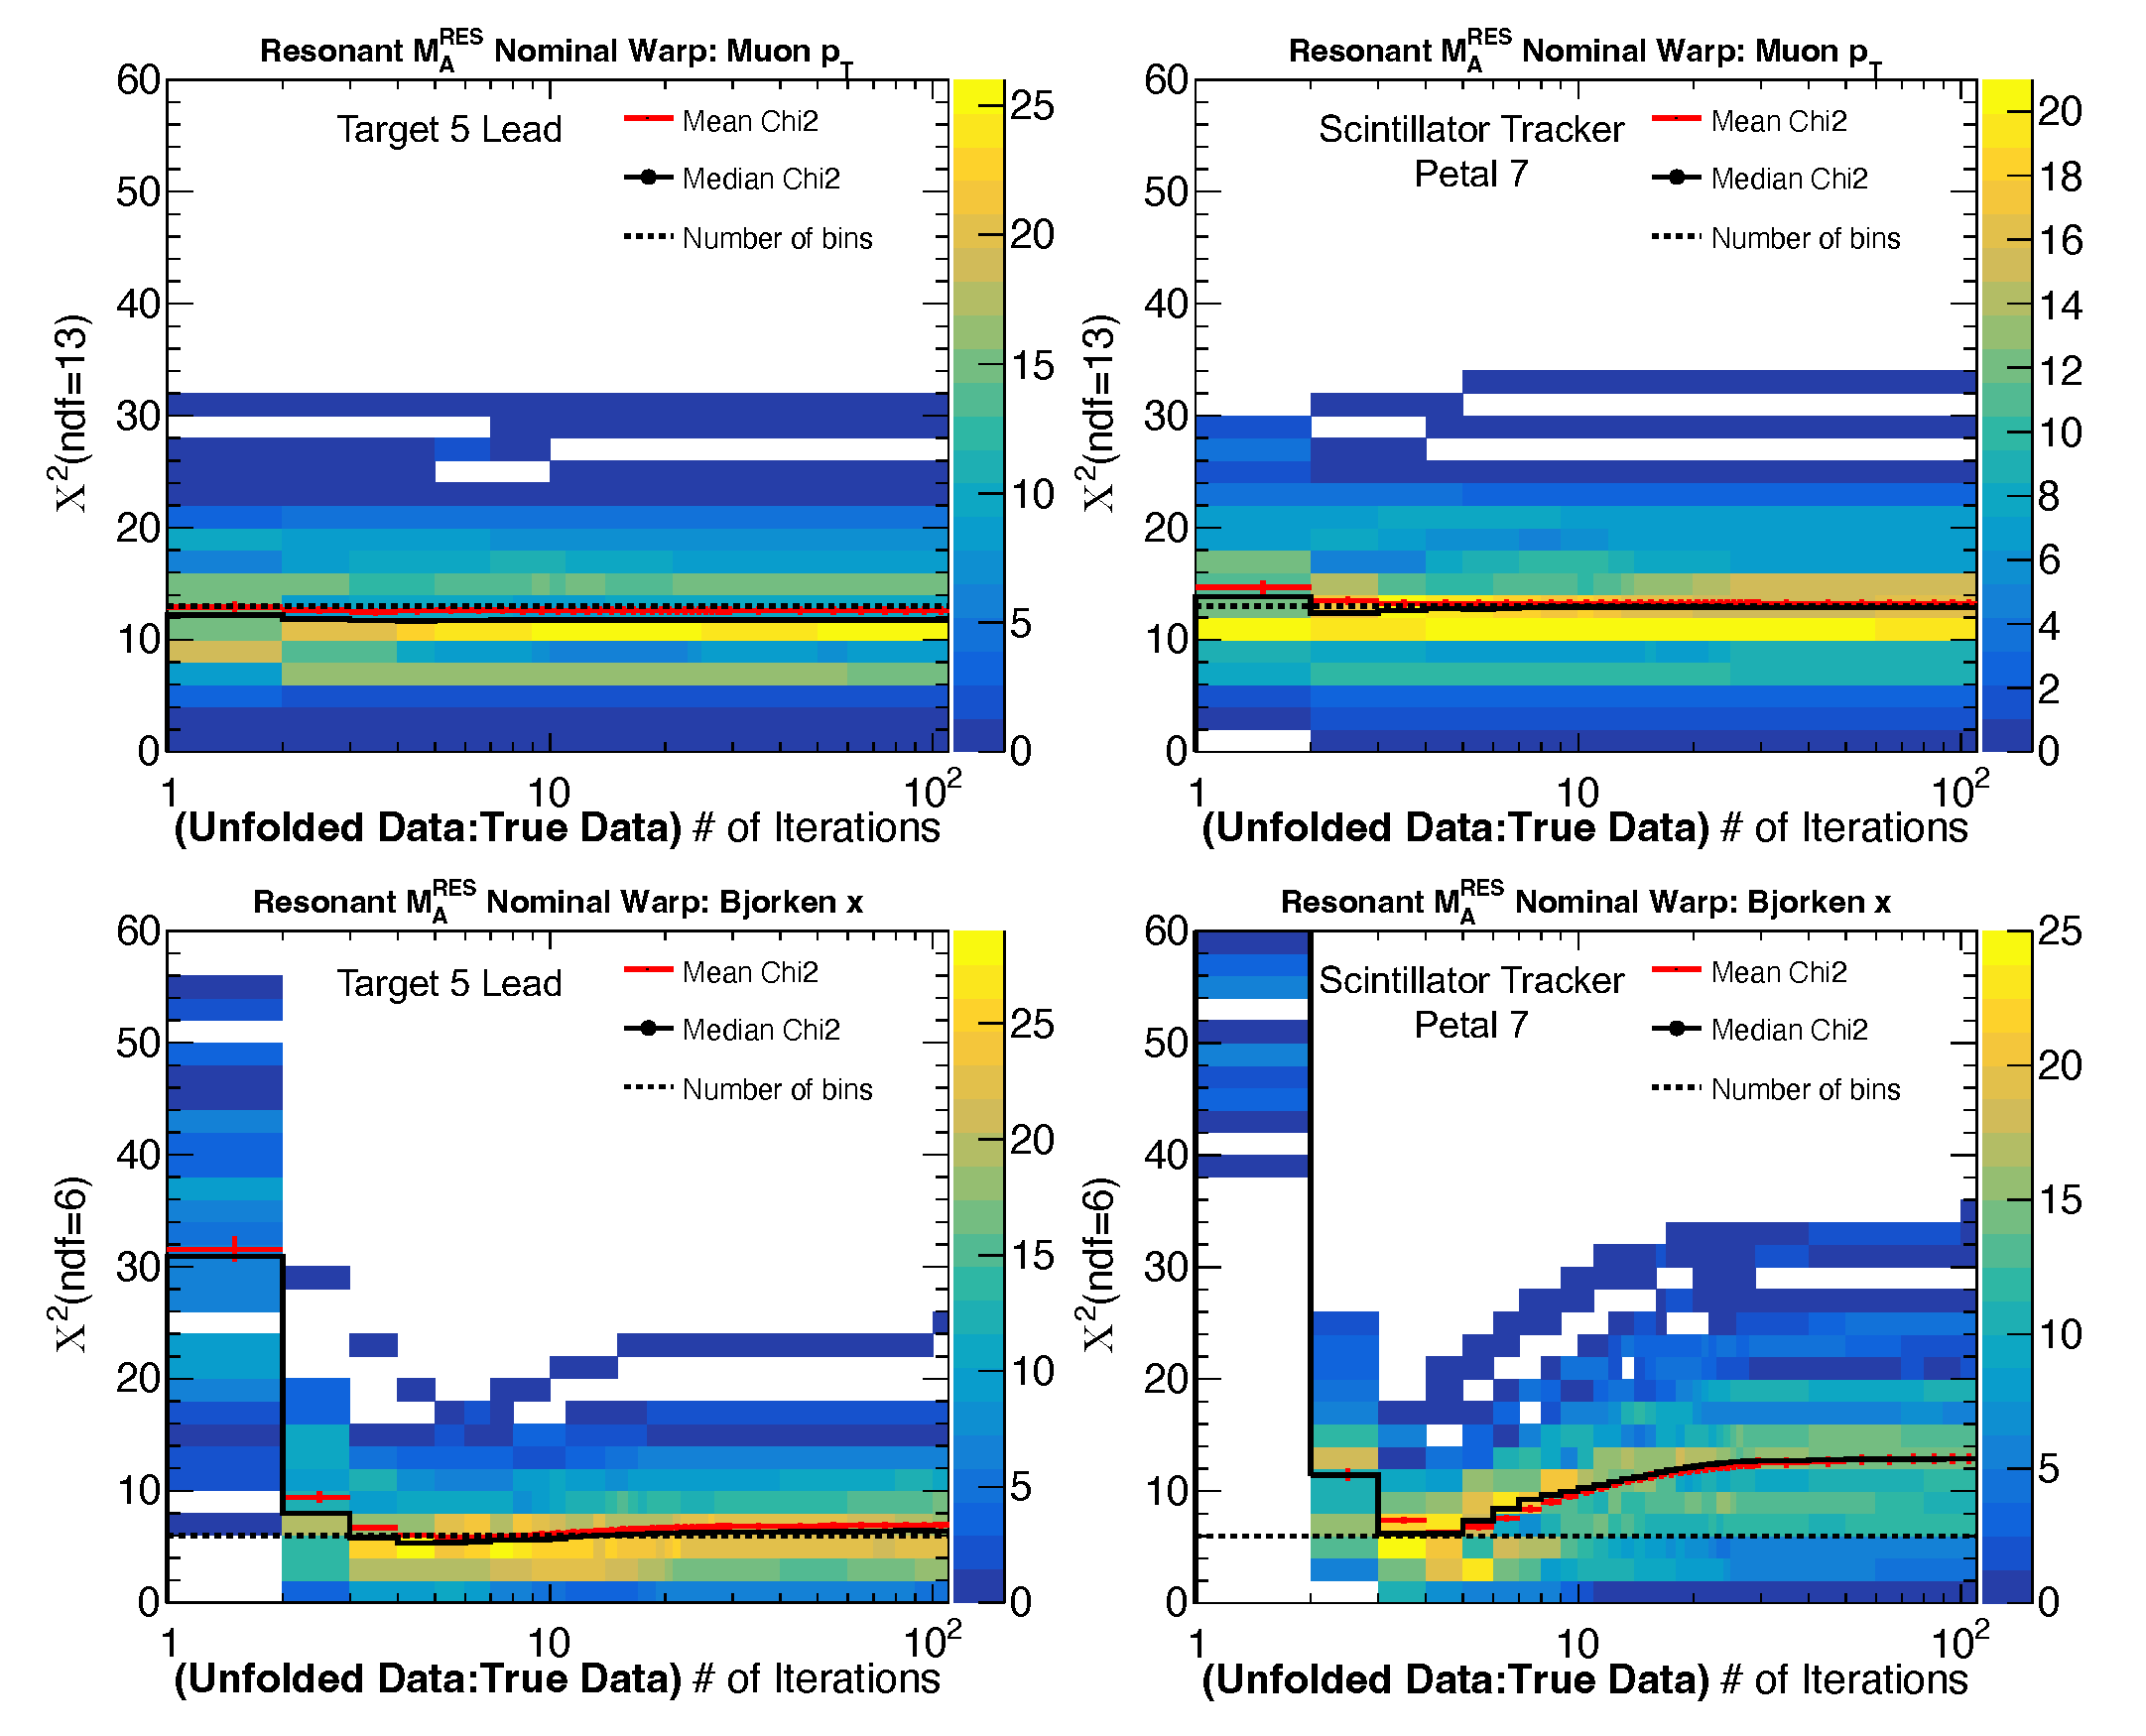
\includegraphics[width=1\textwidth]{07analysis1D/figures/maresWarp_lead5tracker7_pTx.pdf}}%
    \caption{The 'Resonant $M_{A}^{\text{RES}}$ nominal' warping study conducted for target 5 lead (left panel) and the scintillator tracker petal 7 (right panel) in both antimuon $p_{\text{T}}$ (top) and Bjorken $x$ (bottom). Each heatmap displays the calculated $\chi^2$ between the unfolded and true distribution of the warped model as a function of the number of iterations for each of the 100 Poisson throws. The solid lines represent the median and mean $\chi^2$, while the dashed line indicates the number of bins or degrees of freedom (ndf). In $p_{\text{T}}$, the median $\chi^2$ quickly approaches the ndf, signalling minimal bias. In contrast, the median $\chi^2$ for Bjorken $x$ converges to the ndf more gradually. The bottom right heatmap for the scintillator tracker petal 7 exhibits a 'check-mark' shape, indicating convergence to a minimum and then a slight divergence. This pattern prompted further investigation into potential model dependence.}
    %[short caption] {long caption}
    \label{fig:warpingMaRes}
\end{figure}

An example of the `Resonant $M_{A}^{\text{RES}}$ nominal' warping study for target 5 lead and the scintillator tracker petal 7 both in antimuon $p_{\text{T}}$ and Bjorken $x$ is shown in Figure~\ref{fig:warpingMaRes}. While the median $\chi^2$ for $p_{\text{T}}$ is not very far off from the number of degrees of freedom to begin with and converges almost immediately, the Bjorken $x$ median $\chi^2$ has the typical shape of a warping study---each iteration brings the $\chi^2$ closer to the number of degrees of freedom. Furthermore, the scintillator tracker petal 7 distribution in Bjorken $x$ has a `check-mark' shape, where the median $\chi^2$ dips to a minimum at the number of degrees of freedom and then slightly diverges to about twice the number of degrees of freedom over several iterations. To investigate the potential model dependence (and given this is not a blind analysis), the data cross-section was extracted with the warped model as an alternative central value employing the standard cross-section extraction procedure described in this chapter with 9 iterations of unfolding for Bjorken $x$ as listed in the Table~\ref{table:unfoldingIterations}. The data cross-section unfolded with this alternative model was compared to the cross-section extracted with the original simulation to show that the central values of the alternative model are covered by the total (and also just the systematic---outer error bars) uncertainty, and hence any potential model dependence is accounted for by the overall uncertainty. For clarity, this is demonstrated in Figure~\ref{fig:maresCheck_invisECheck} as a lead-to-scintillator cross-section ratio with the individual cross-section comparisons and other cross-section ratio comparisons included in the Appendix~\ref{ch:appendix_unfoldingStudies}.

\begin{figure}[t!] 
    \centering
    {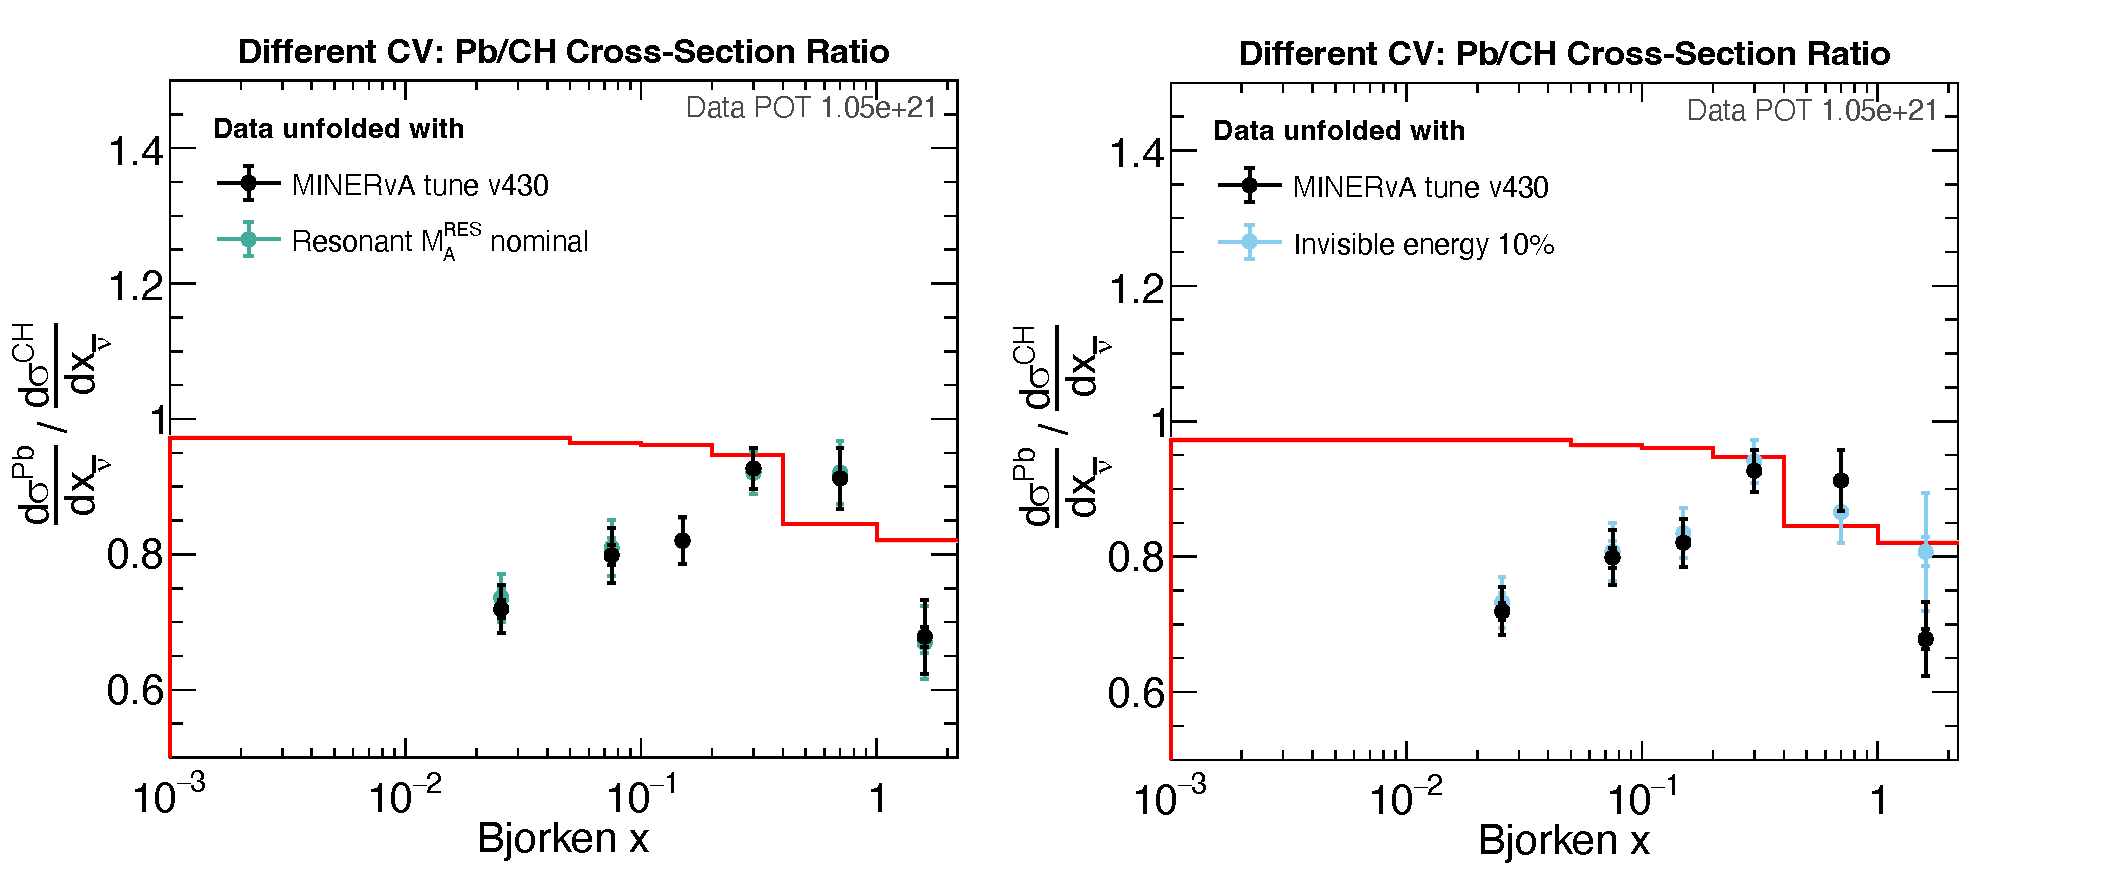
\includegraphics[width=1\textwidth]{07analysis1D/figures/maresCheck_invisECheck.pdf}}%
    \caption{Left: Comparison of the lead-to-scintillator data cross-section ratio extracted with the underlying simulation MINERvA tune v430 and the warped model `Resonant $M_{A}^{\text{RES}}$ nominal' as a function of Bjorken $x$. The central values of the data cross-section extracted using the warped model are encompassed by the total uncertainty (including the systematic, represented by the outer error bars) of the data cross-section extracted using the original simulation. This indicates that any potential model dependence is covered by the underlying uncertainty. Right: Comparison of the  lead-to-scintillator data cross-section ratio as a function of Bjorken $x$ extracted with the original simulation and `Invisible energy 10\%' central value to investigate model dependence arising from neutron modelling, revealing possible bias in the $x > 1$ bin.}
    %[short caption] {long caption}
    \label{fig:maresCheck_invisECheck}
\end{figure}

The `SuSA 2p2h' warping study for the same targets (target 5 lead and the scintillator tracker petal 7) in both $p_{\text{T}}$ and Bjorken $x$ is also shown in the Figure~\ref{fig:warpingSuSA_pulls} using the calculated mean of the pull distribution in each bin at various numbers of iterations. The pull of a kinematic distribution in each bin $i$ is defined as
\vspace{-10pt}
\begin{equation}
    \label{eq:pulls}
    \vspace{-10pt}
    \text{pull}_{i} = \frac{(\text{reco}-\text{true})_i}{\sigma_{i}^{\text{true}}},
\end{equation}
where `reco' is the reconstructed value, `true' is the unfolded value and $\sigma_{i}^{\text{true}}$ is the uncertainty on the unfolded value in the given bin $i$. This visualisation of the warping study also illustrates that the `SuSA 2p2h' warped model can be unfolded using the central value migration matrix for both $p_{\text{T}}$ and Bjorken $x$. The pull distributions nicely represent how with each iteration the unfolding gets less biased, i.e. the mean of the pull distribution in every bin gets closer to zero. The equivalent distribution to Figure~\ref{fig:warpingMaRes} for the `SuSA 2p2h' warped model and the pull distribution for the `Resonant $M_{A}^{\text{RES}}$ nominal' warp are included in the Appendix~\ref{ch:appendix_unfoldingStudies}.

\begin{figure}[b!] 
    \centering
    {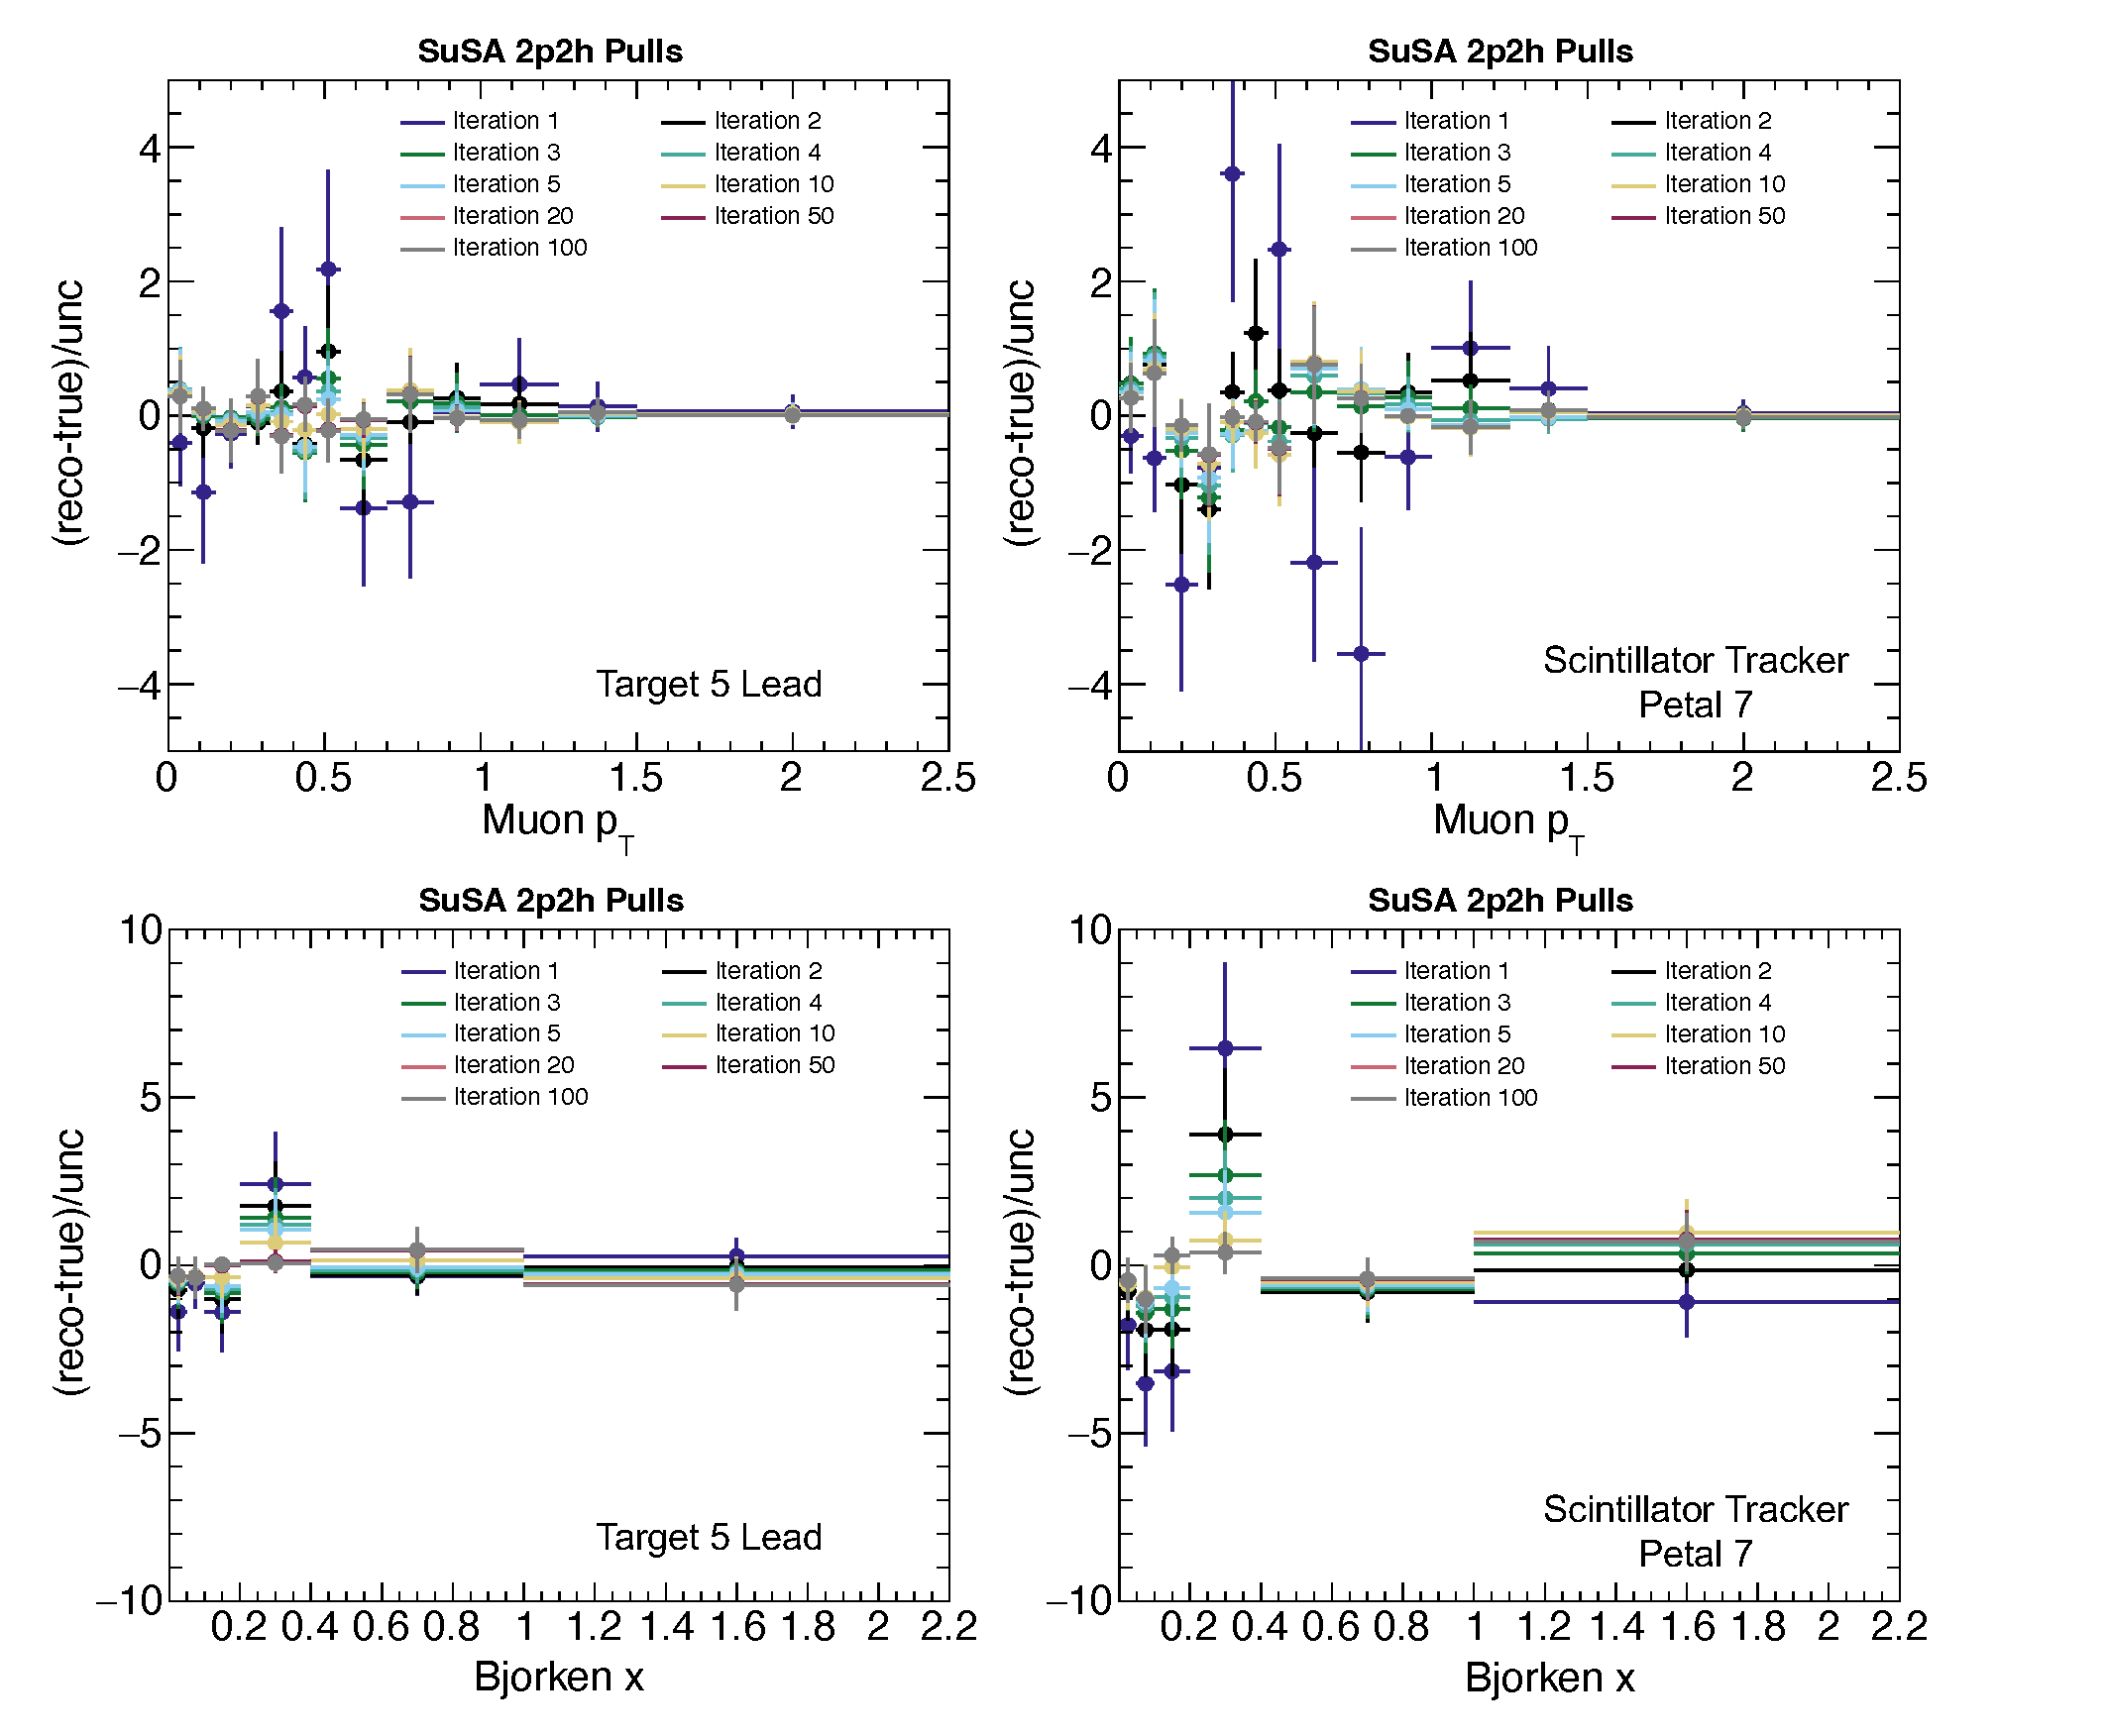
\includegraphics[width=1\textwidth]{07analysis1D/figures/susaWarp_lead5tracker7_pTx_pulls.pdf}}%
    \caption{Pull distributions for the 'SuSA 2p2h' warping study for target 5 lead (left panel) and the scintillator tracker petal 7 (right panel) in both antimuon $p_{\text{T}}$ (top) and Bjorken $x$ (bottom). Each pull distribution illustrates the reduction in bias with each iteration of the unfolding process.~In other words, the mean of the pull distribution in each bin converges toward zero.}
    %[short caption] {long caption}
    \label{fig:warpingSuSA_pulls}
\end{figure}

Apart from the warping studies detailed in Table~\ref{table:warpingList}, an additional simple study was conducted to evaluate the potential bias introduced by neutron production in antineutrino interactions in this analysis.~This is particularly relevant as antineutrino interaction generators are typically employed to correct for these effects, given that most of the energy deposited by neutrons in detectors is invisible. However, a recent MINERvA measurement of multi-neutron cross-sections showed disagreement with predictions from several leading models \cite{MINERvA:2023ikp}. Hence, the neutron modelling corrections introduced at the unfolding level could impact the Bjorken $x$ distribution, especially in the high $x$ region, where they are coupled with the already inherently challenging modelling of the $x > 1$ region mentioned earlier in this chapter.

Thus, the strategy was to examine how a change at the true level of the simulation (and not the reconstructed) impacts the analysis.~Naïvely, this was accommodated by introducing additional invisible energy into the system, achieved by increasing the true antineutrino energy by 10\% of the true invisible energy while keeping the muon system intact. Similar to the investigation of the bias in the case of the `check-mark' shaped warping study discussed above, the data cross-section was extracted with this new model using 9 iterations of unfolding for Bjorken $x$ and compared to the cross-section extracted using the original simulation. The lead-to-scintillator cross-section ratio in Figure~\ref{fig:maresCheck_invisECheck} shows that the central values of the alternative model are covered by the total uncertainty, except for the last $x > 1$ bin. This potential source of model bias requires further action, and the possibility of including an additional source of systematic uncertainty related to neutron modelling is discussed in Chapter~\ref{ch:systematics}. The individual cross-section comparisons and the other cross-section ratio comparisons can be found in Appendix~\ref{ch:appendix_unfoldingStudies}.

\begin{figure}[t!] 
    \centering
    {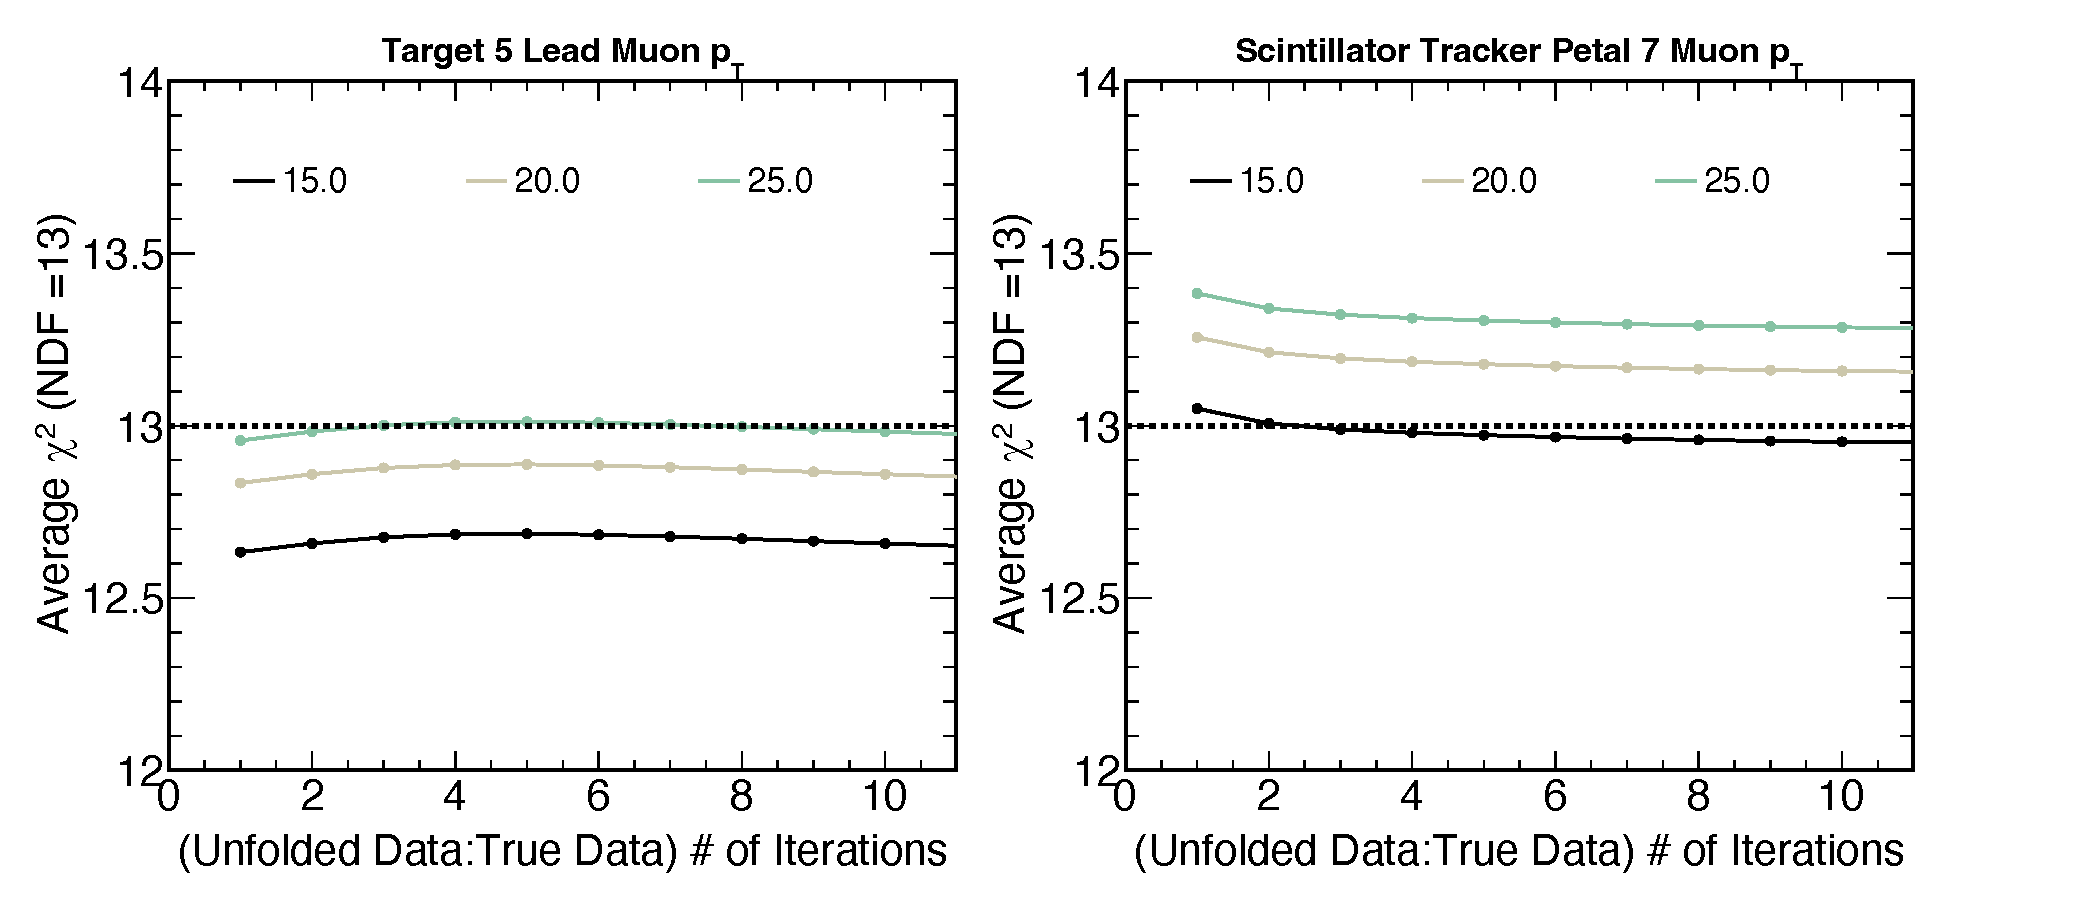
\includegraphics[width=1\textwidth]{07analysis1D/figures/additionalStatUnc_lead5tracker7_pT.pdf}}%
    \caption{Correction factor $F$ to the statistical uncertainty of the unfolded sample due to finite size of the simulation in the migration matrix for target 5 lead and the scintillator tracker petal 7 in antimuon $p_{\text{T}}$. The solid lines illustrate that at the selected number of iterations, i.e. 3 iterations, the calculated $\chi^2$ between the unfolded and true simulation converges to the number of degrees of freedom (dashed line) for the $F$ factor 25 and 15 for the target 5 lead and the scintillator tracker petal 7 respectively.  }
    %[short caption] {long caption}
    \label{fig:additionalStatUnc_pT}
\end{figure}

Finally, RooUnfold's implementation of the D'Agostini unfolding doesn't take into account uncertainties in the response matrix due to the finite statistics of the simulation sample~\cite{Adye:2011gm}. This leads to an underestimation of the statistical uncertainty of the unfolded sample and can be particularly significant for large sample analyses such as this one. To address this issue, a correction factor to the statistical uncertainty related to the relative simulation-to-data fraction, i.e.~about 4.43 for the antineutrino dataset used in this analysis, was implemented. 

% https://minerva-docdb.fnal.gov/cgi-bin/sso/RetrieveFile?docid=28899&filename=MINERvA_Unfolding_AMatterOfUncertainty.pdf&version=1
% https://minerva-docdb.fnal.gov/cgi-bin/sso/RetrieveFile?docid=28992&filename=MINERvA_Unfolding_AMatterOfUncertainty_FollowUp_Collaboration.pdf&version=2

In order to do so, a new migration matrix was constructed by Poisson throwing each bin of the original migration matrix as a fraction of data exposure. Then, the new reconstructed simulation coming from the projection of the new migration matrix was unfolded with this new migration matrix and compared to the original true \mbox{simulation~\cite{StatCorrFactor,StatCorrFactor2}}. The statistical covariance of the unfolded sample was multiplied by $\sqrt{(1+1/F)}$, where $F$ is the correction factor. 
A search over various $F$ factors for the given fraction of data exposure was performed such as the calculated $\chi^2$ between the unfolded sample with the corrected statistical covariance and the original true distribution corresponded to the number of degrees of freedom at the number of iterations selected. Figure~\ref{fig:additionalStatUnc_pT} illustrates the correction factors $F$ for the antimuon $p_{\text{T}}$ distributions in target 5 lead and the scintillator tracker petal 7, which are 25 and 15 respectively. The correction factors for the equivalent Bjorken $x$ distributions are included in Appendix~\ref{ch:appendix_unfoldingStudies}.

[unfolded distribution plots]


% Check-marked warps
%https://minerva-docdb.fnal.gov/cgi-bin/sso/RetrieveFile?docid=31954&filename=2023-08-24-update.pdf&version=1
% https://minerva-docdb.fnal.gov/cgi-bin/sso/RetrieveFile?docid=31960&filename=2023-09-01-update.pdf&version=1
% invisible enrrgy scale
% https://minerva-docdb.fnal.gov/cgi-bin/sso/RetrieveFile?docid=32074&filename=06-10-2023-collabMeeting.pdf&version=2


% Regularization is achieved by stopping iterations before reaching the ‘true’ (but wildly fluctuating) inverse. The regularization parameter is just the number of iterations. In principle, this has to be tuned according to the sample statistics and binning. In practice, the results are fairly insensitive to the precise setting used.
% RooUnf


% Dolan et al for SuSA https://journals.aps.org/prd/abstract/10.1103/PhysRevD.101.033003
% Ascencio et al for SuSA reweight R. Gran, A. B. & Ascencio, M. Implementation of SuSA 2p2h and QE weights for MINERvA tech. rep. 29414 (MINERvA Collaboration, July 2021).
% Gran, R. SuSA 2p2h and QE as weights to our MC tech. rep. 25386 (MINERvA Collaboration, Dec. 2019).

% Cowan, G. Statistical Data Analysis (Oxford University Press Distribution Services North Kettering Business Park Hipwell Road Kettering Northants NN14 1UA, 1998).
% https://indico.cern.ch/event/107747/contributions/32645/attachments/24317/35000/blobel.pdf


\iffalse
\fi
\newpage
\section{Efficiency correction}
\label{ch:efficiency}

Due to the limitations of the detector's acceptance and the imperfect reconstruction, it is impossible to detect and reconstruct every signal event that occurs in the detector. Both of these effects result in reducing the number of signal events in the final sample. As~such, they need to be accounted for in the cross-section calculation by applying an efficiency correction derived from the simulation. Specifically, the background-subtracted signal events, which were unfolded to the detector-independent quantities as detailed in the preceding section, are divided by the efficiency correction $E_{\alpha}$ as outlined in the Equation~\ref{eq:xsec1D}.

The efficiency correction $E_{\alpha}$ in each bin $\alpha$ for a given analysis variable distribution is defined as
\begin{equation}
    \label{eq:efficiency}
    E_{\alpha} = \frac{N_{\alpha}^{\text{Generated and reconstructed signal events}}}{N_{\alpha}^{\text{All generated signal events}}},
\end{equation}
relying on the simulation sample containing both the true generated and the reconstructed information about the simulated events. Due to differences in target geometries and positions, the efficiency has to be calculated separately for each of them. By definition, $E_{\alpha}$ is always less than one.

\begin{figure}[b!]
    \centering
    {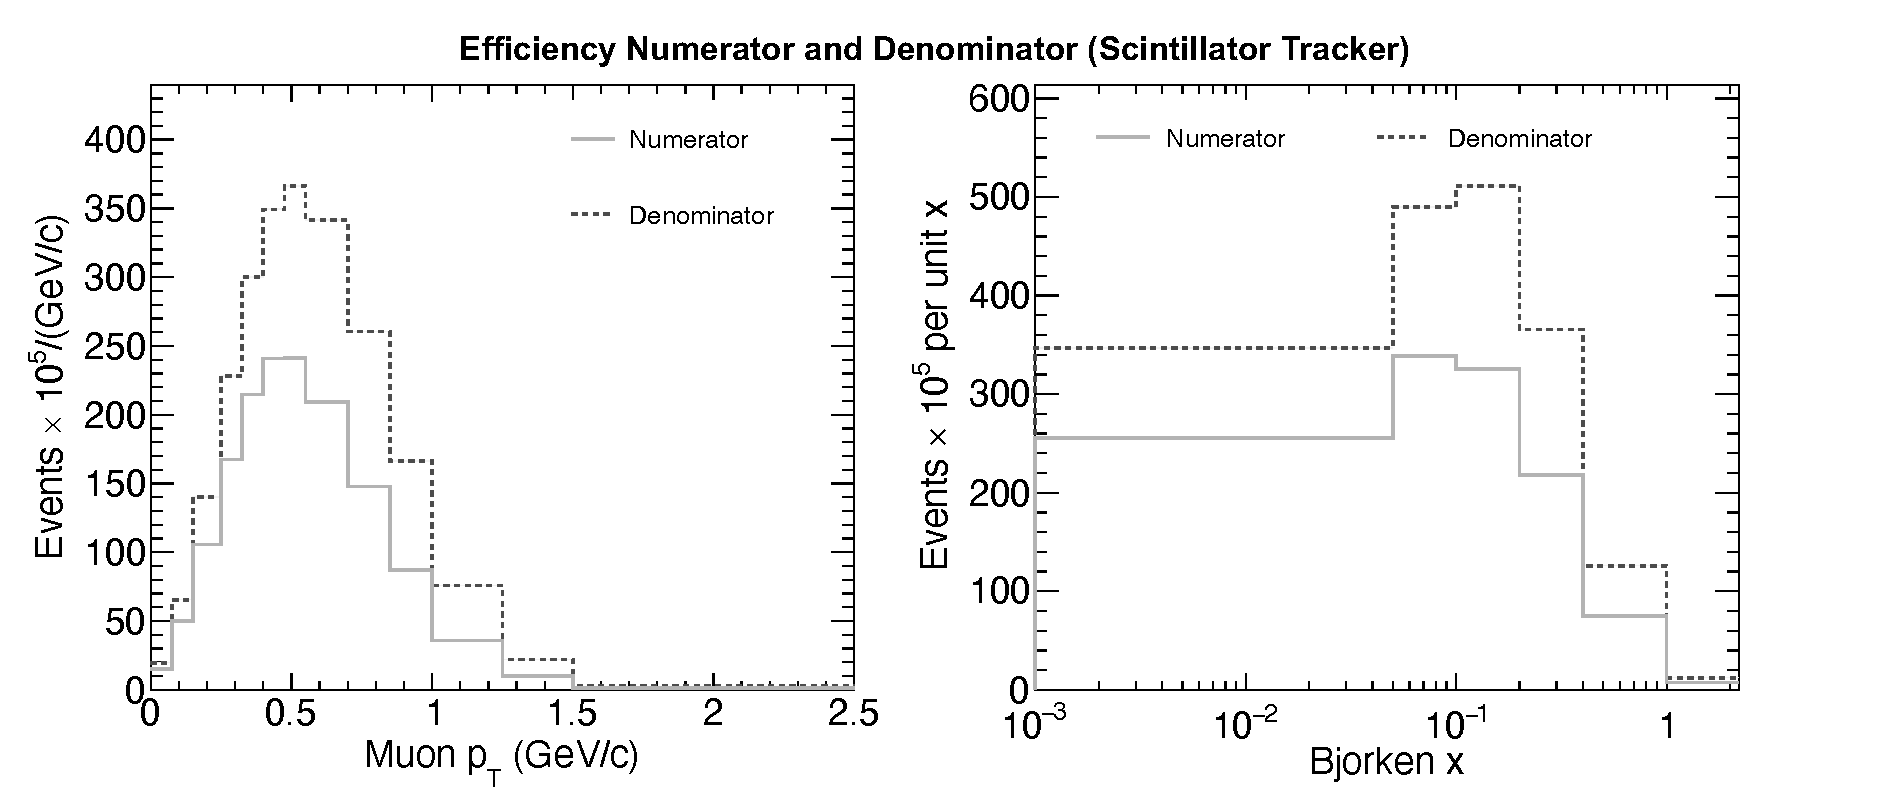
\includegraphics[width=1\textwidth]{07analysis1D/figures/efficiency_trackerNumDenom_pTx.pdf}}%
    \caption{Efficiency numerator and denominator distributions for the scintillator tracker in both $p_{\text{T}}$ (left) and Bjorken $x$ (right). The solid line for the numerator represents the generated and reconstructed signal events, while the dashed line for the denominator denotes the superset of all generated signal events.}
    %[short caption] {long caption}
    \label{fig:efficiencyNumDenom_scintillatorTracker_pTx}
\end{figure}

In practice, this means filling two histograms representing the numerator and the denominator in Equation~\ref{eq:efficiency} using the true information of the events and taking their ratio. An example of these two histograms used in the calculation of the scintillator tracker efficiency for both $p_{\text{T}}$ and Bjorken $x$ is shown in Figure \ref{fig:efficiencyNumDenom_scintillatorTracker_pTx}. While the numerator events are selected from the subsample of the reconstructed events and hence carry the systematic uncertainties associated with the detector's acceptance and event reconstruction, the denominator events are independent of them. This is demonstrated in Figure \ref{fig:efficiencyNumDenom_fracUnc} showing the systematic uncertainties of both the efficiency numerator and the denominator for the scintillator tracker as a function of $p_{\text{T}}$. 


\begin{figure}[b!]
    \centering
    {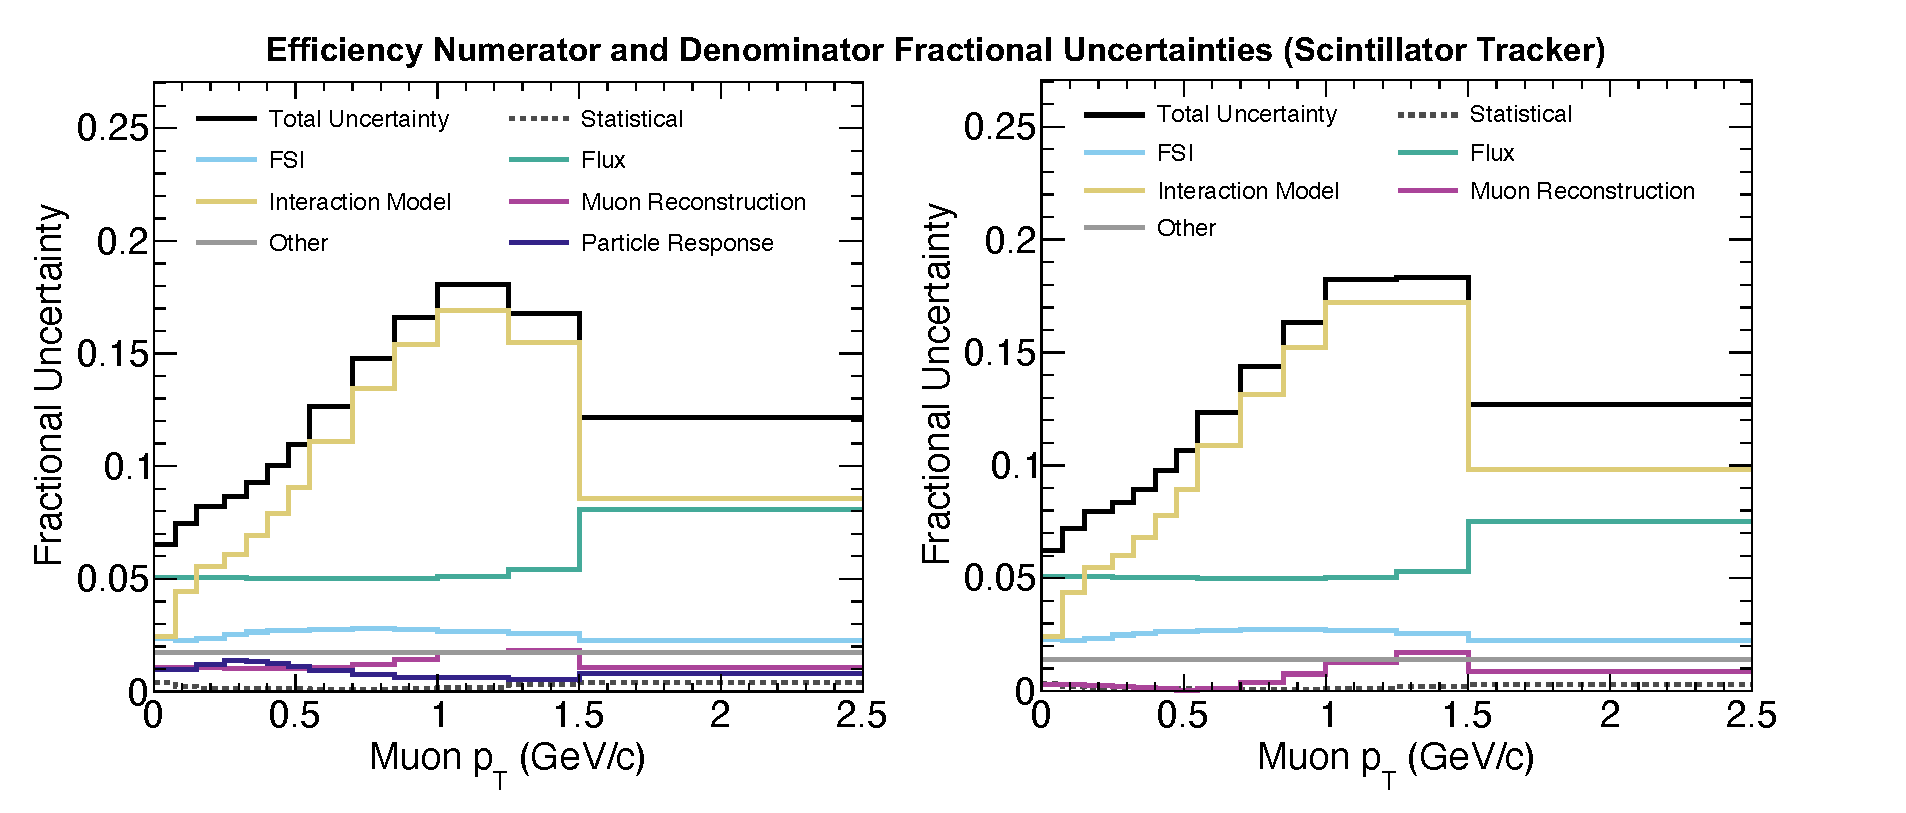
\includegraphics[width=1\textwidth]{07analysis1D/figures/efficiency_trackerNumDenomFracUnc_pT.pdf}}%
    \caption{Fractional uncertainty breakdown for the efficiency numerator (left) and the denominator (right) distributions of scintillator tracker as a function of $p_{\text{T}}$. Note the omitted `Particle Response' uncertainty band and the reduced `Muon Reconstruction' uncertainty band in the denominator uncertainty on the right.  }
    %[short caption] {long caption}
    \label{fig:efficiencyNumDenom_fracUnc}
\end{figure}

Specifically, Figure \ref{fig:efficiencyNumDenom_fracUnc} highlights that the denominator fractional uncertainty does not include the uncertainty linked to the calorimetric energy response of the detector and interaction cross-sections of particles traversing through the detector, represented by the `Particle Response' uncertainty band. The `Muon Reconstruction' uncertainty band omits all uncertainty sources except for those related to the MINOS antimuon momentum universes, which are directly correlated with flux. Finally, the `Other' uncertainty band is reduced by excluding the uncertainty associated with vertex reconstruction. A detailed description of the various systematic uncertainty bands can be found in Chapter~\ref{ch:systematics}.
%  The flux is different in the MINOS-muon-momentum-shifted universes, which means it should have an effect anywhere the Flux universes have an effect. 

\begin{figure}[b!]
    \centering
    {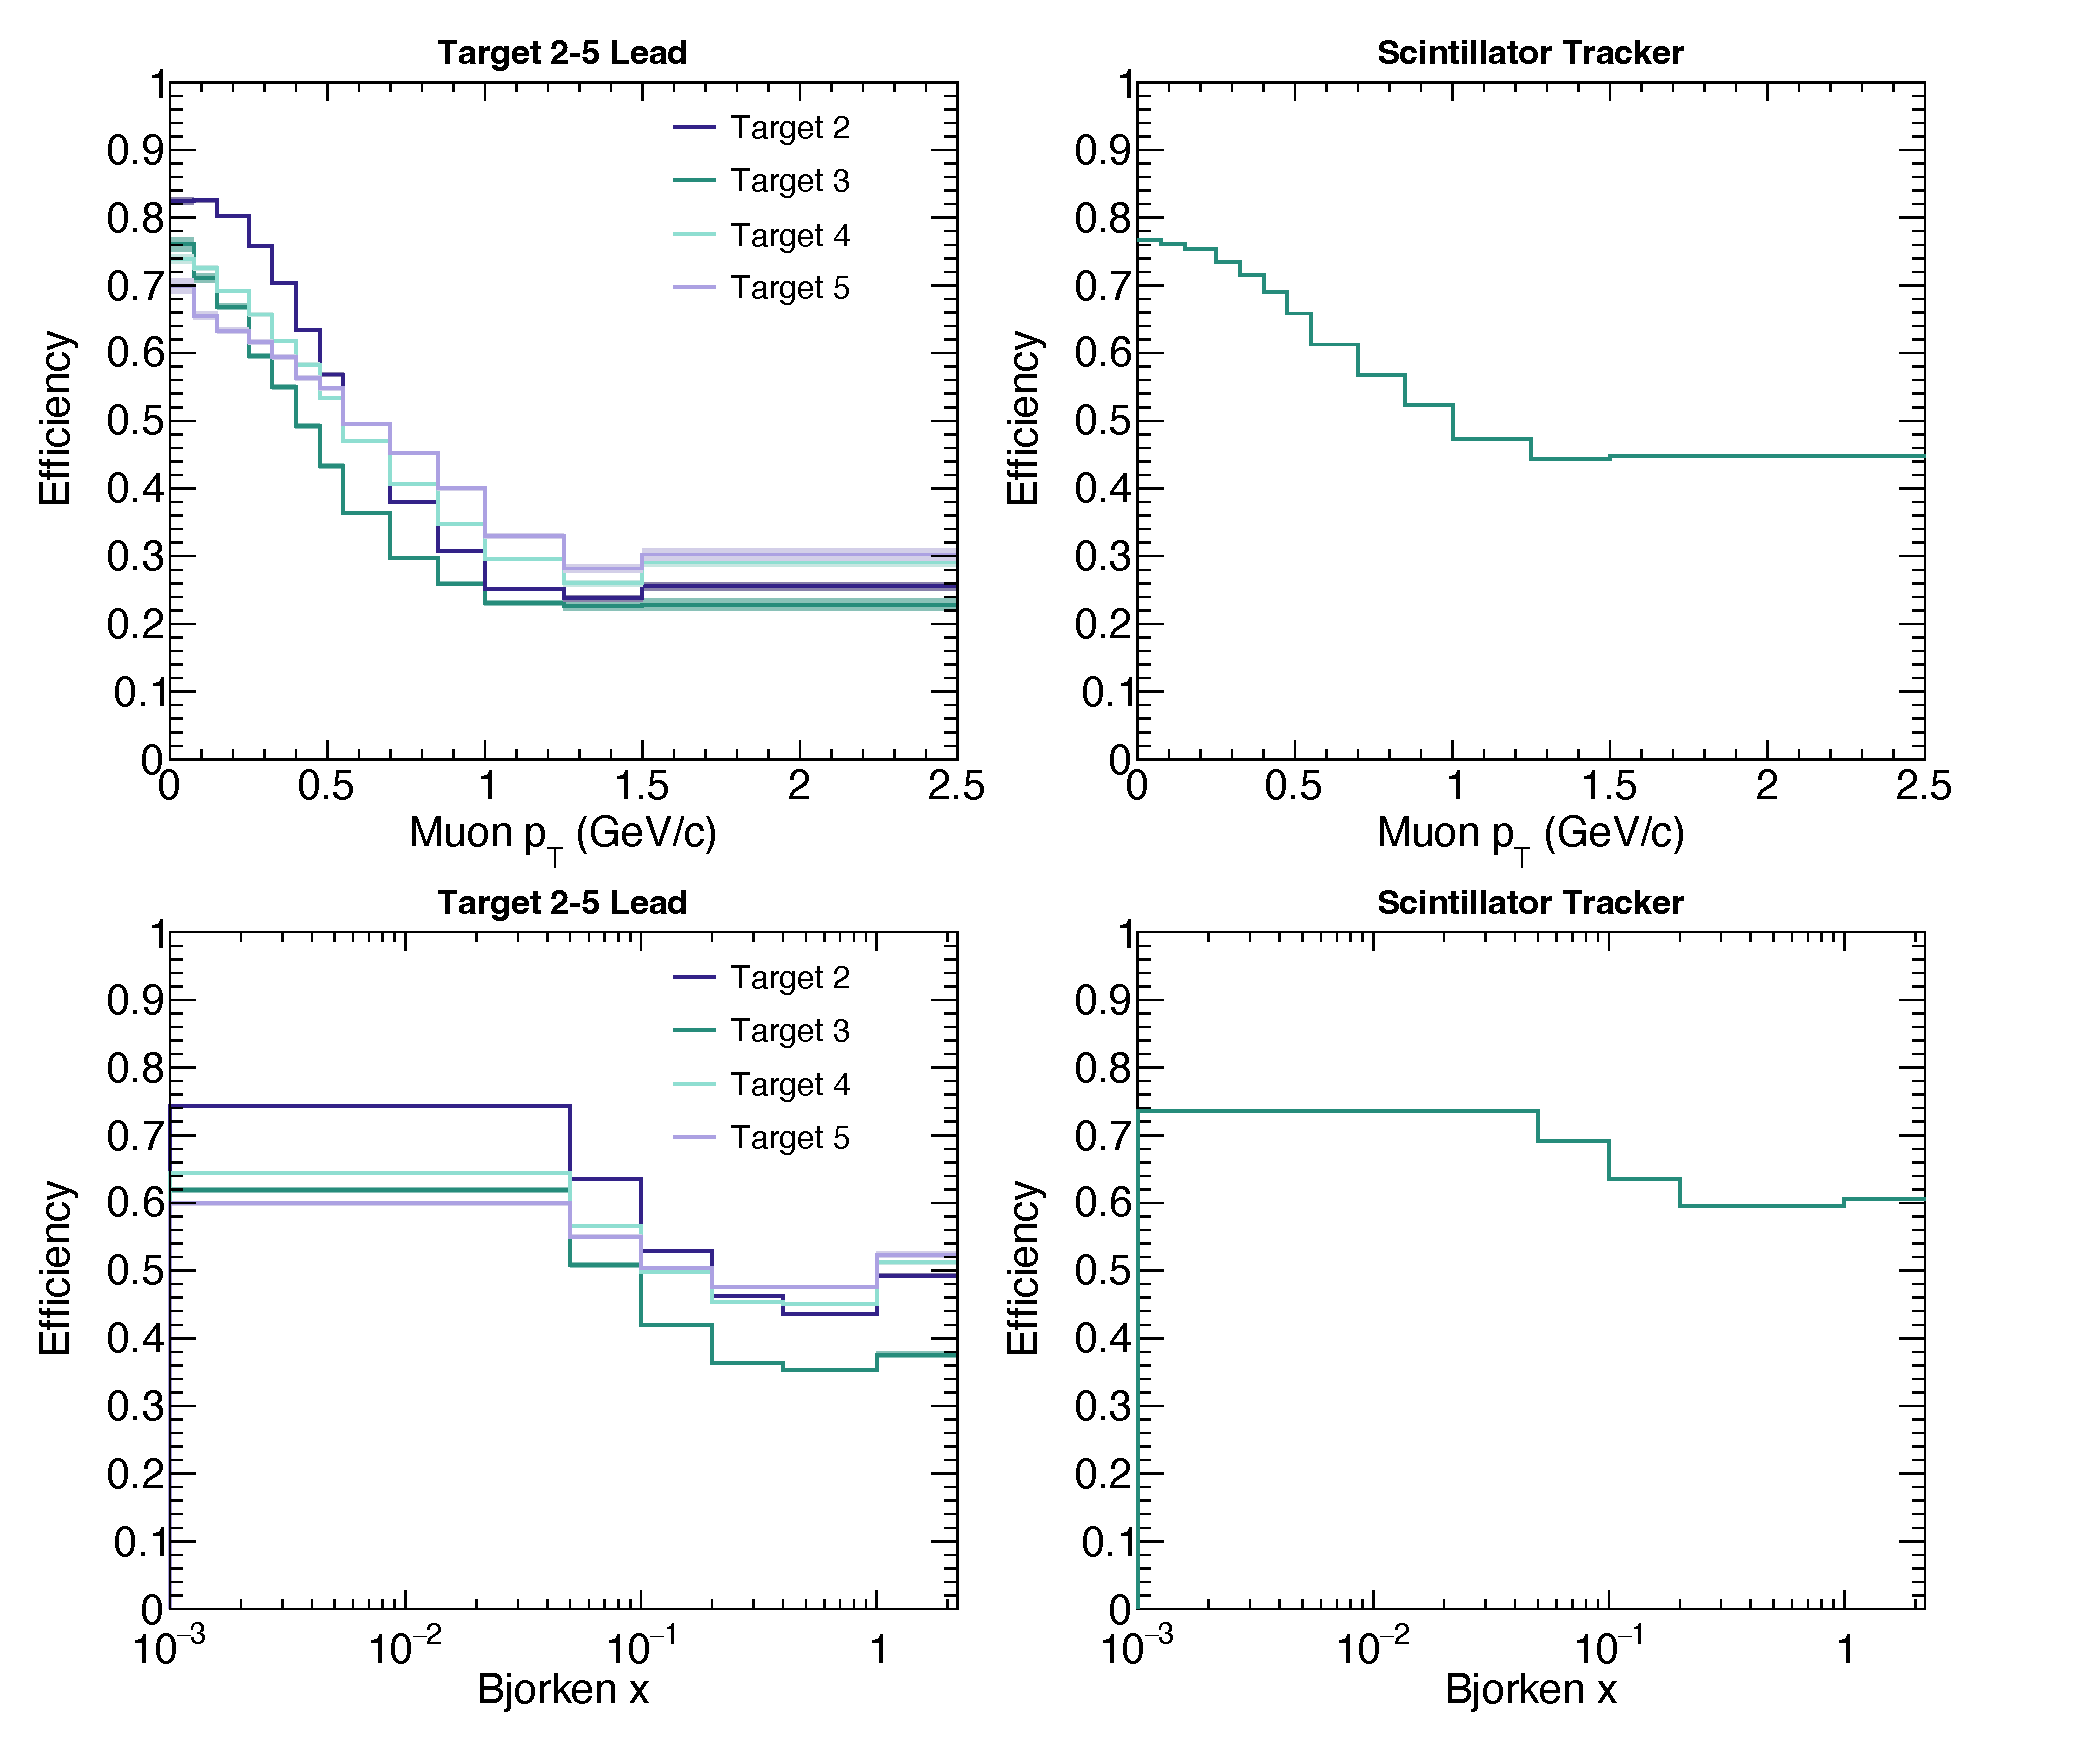
\includegraphics[width=1\textwidth]{07analysis1D/figures/efficiency_lead_tracker_pTx.pdf}}%
    \caption{Efficiency correction distributions for the various lead targets (left panel) and the scintillator tracker (right panel) as a function of $p_{\text{T}}$ (top) and Bjorken $x$ (bottom).}
    %[short caption] {long caption}
    \label{fig:efficiency_lead_tracker_pTx}
\end{figure}

Because the numerator distribution of the selected reconstructed events is a subsample of the denominator distribution of the selected generated events, the two distributions are correlated and so are their systematic uncertainties, as indicated by Figure \ref{fig:efficiencyNumDenom_fracUnc}. Consequently, when calculating the ratio, the correlations between the uncertainties are taken into account by using binomial error propagation. The efficiencies for different lead targets and the scintillator tracker both in $p_{\text{T}}$ and Bjorken $x$ are shown in Figure \ref {fig:efficiency_lead_tracker_pTx}. 

% Binomial error
% fSumw2.fArray[bin] = TMath::Abs( ( (1-2*w)*e1*e1 + w*w*e2*e2 )/(b2*b2) );  
% where w = b1/b2

Due to the inclusive nature of the analysis, the efficiency relies on detecting and reconstructing the antimuon both in the MINERvA detector and the MINOS spectrometer. The top panel of Figure \ref{fig:efficiency_lead_tracker_pTx} illustrates the fall-off in the $p_{\text{T}}$ efficiency at higher $p_{\text{T}}$. This is attributed to the fact that $p_{\text{T}}$ serves as a proxy for the antimuon angle, whose detection is constrained by the limited antimuon acceptance of the MINOS spectrometer at higher angles. Furthermore, the differences between the various lead target efficiencies in Figure~\ref{fig:efficiency_lead_tracker_pTx} can be explained due to their positions in the detector with respect to the MINOS spectrometer.

For example, target 2 lead is more upstream than target 5 lead. At lower $p_{\text{T}}$ (antimuon angle), the antimuon is likely to be more energetic than at higher $p_{\text{T}}$. This means that a~more energetic antimuon produced by an interaction in target 2 lead has to traverse more material before reaching the MINOS spectrometer and loses more energy compared to one produced in target 5 lead. Therefore, the antimuon from target 2 lead is more likely to be able to stop in the MINOS spectrometer and be reconstructed, resulting in target 2 lead having higher $p_{\text{T}}$ efficiency than target 5 lead. Conversely, an antimuon produced with a higher angle in a target more downstream and thus closer to the MINOS spectrometer is more likely to be reconstructed. This leads to target 5 lead having a~larger efficiency at higher $p_{\text{T}}$ compared to target 2 lead.

The Bjorken $x$ efficiency in the bottom panel of Figure~\ref{fig:efficiency_lead_tracker_pTx} exhibits similar behaviour as $p_{\text{T}}$. Nevertheless, the decline at higher Bjorken $x$ is less pronounced due to the weaker dependence on the antimuon angle. 

\begin{table}[b!]
    \centering

    \begin{tabular}{c c c}
    \hline \\ [-1.5 ex]
    Target & Material & Efficiency (\%) \\ [0.5ex] % inserts table %heading
    \hline
    \hline
    2 & Iron & 41.9 \\
      & Lead & 49.5 \\
    \hline
    3 & Carbon & 52.4 \\
      & Iron & 40.3 \\
      & Lead & 39.7 \\
    \hline
    4 & Lead & 47.8 \\
    \hline
    5 & Iron & 50.5\\
      & Lead & 48.8 \\
    \hline
    Tracker & Scintillator & 63.3 \\
    \hline
    \end{tabular}

    \caption{Integrated efficiency correction for all targets of different materials and the scintillator tracker.}
    \label{table:efficiency}
\end{table}


The integrated efficiency for all the targets of different materials and the scintillator tracker can be found in Table~\ref{table:efficiency}. For targets in particular, the efficiency depends on the ability to reconstruct the vertex in the nuclear target, as detailed in Chapter~\ref{ch:Reconstruction}. Furthermore, within a given target, the efficiency is lower for materials that shadow the MINOS coil described in Chapter~\ref{ch:minerva}, such as iron in the second target or lead in the fifth target.

\begin{figure}[b!] 
    \centering
    {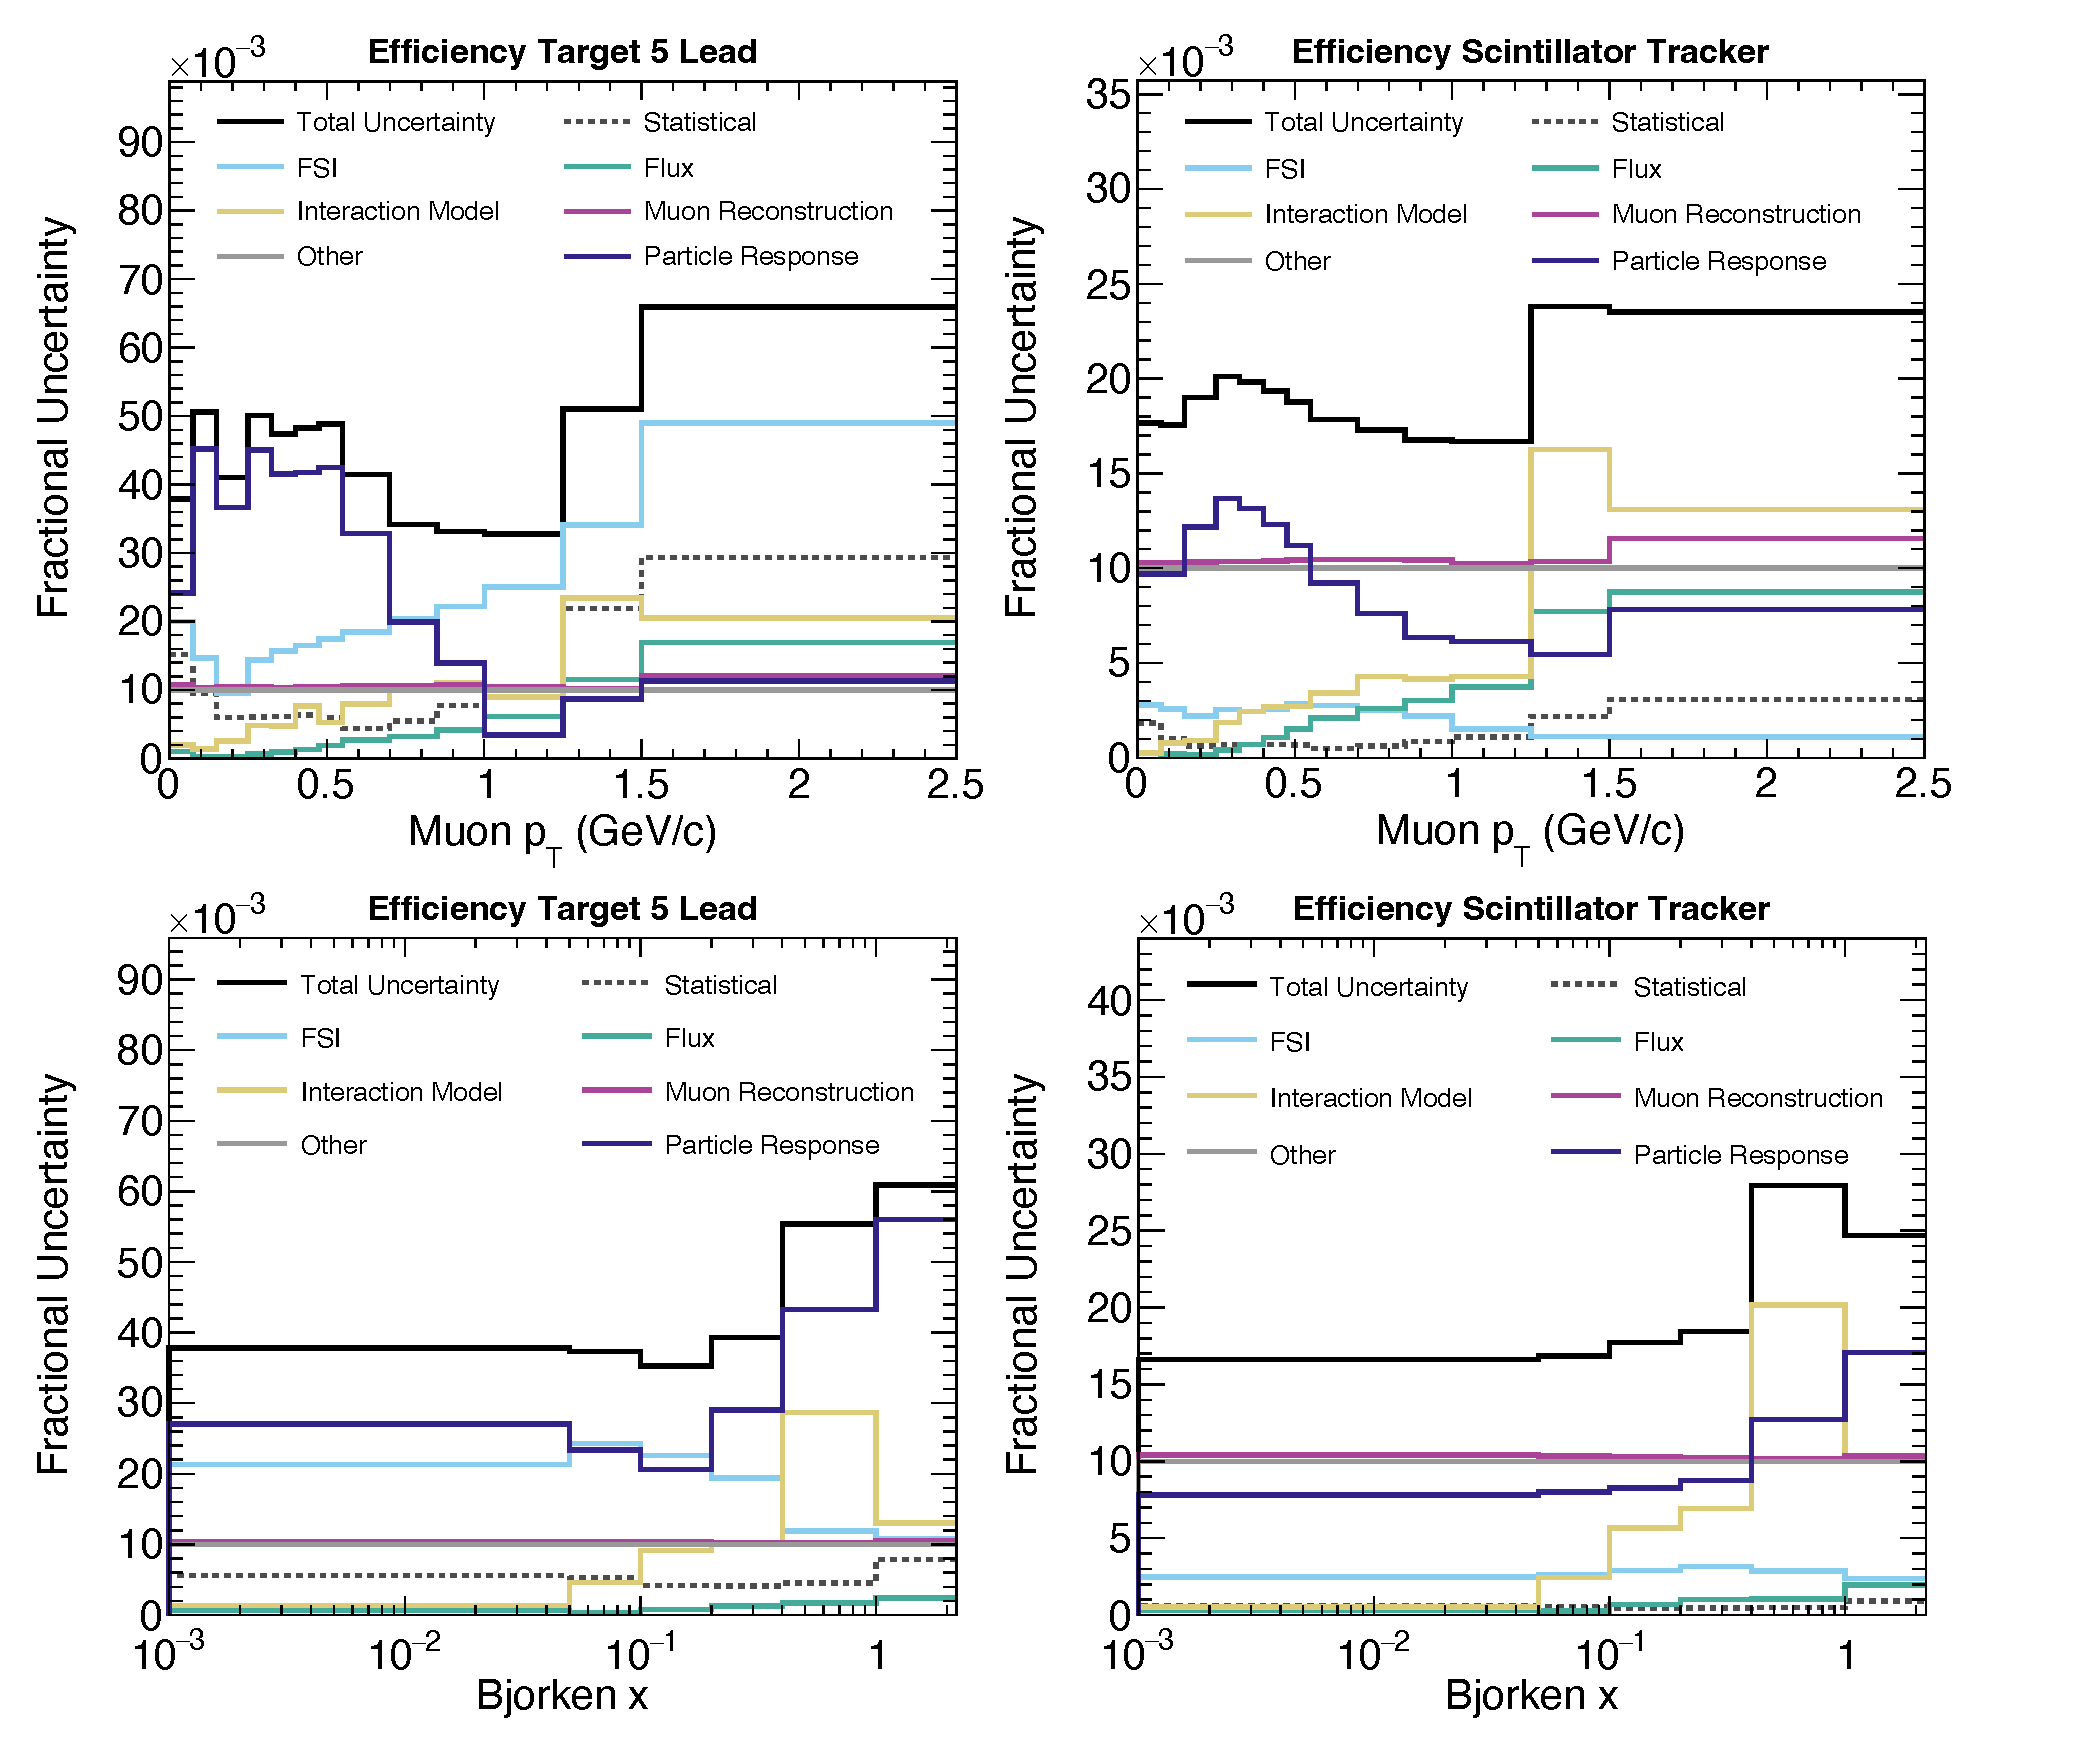
\includegraphics[width=1\textwidth]{07analysis1D/figures/efficiency_lead_tracker_pTx_fracErr.pdf}}%
    \caption{Fractional uncertainty breakdown for the efficiency of target 5 lead (left panel) and scintillator tracker (right panel) as a function of $p_{\text{T}}$ (top) and Bjorken $x$ (bottom). Note the increase in the `FSI' uncertainty band for lead compared to the scintillator. }
    %[short caption] {long caption}
    \label{fig:efficiency_lead_tracker_pTx_fracErr}
\end{figure}

% systematics
The fractional uncertainty on the target 5 lead and scintillator tracker efficiency in both $p_{\text{T}}$ and Bjorken $x$ is shown in Figure~\ref{fig:efficiency_lead_tracker_pTx_fracErr}. The region of low $p_{\text{T}}$ and high Bjorken~$x$, mainly associated with quasi-elastic events, is dominated by the `Particle Response' uncertainty coming from the efficiency numerator. Specifically, this uncertainty is mostly attributed to the uncertainty on the neutron cross-section. Additionally, both high $p_{\text{T}}$ and high Bjorken~$x$ have prominent `Interaction Model' uncertainty bands, primarily arising from the resonance production model. Figure~\ref{fig:efficiency_lead_tracker_pTx_fracErr} also illustrates that the `FSI' uncertainty band is more pronounced the heavier the nucleus is, i.e. heavy lead versus relatively light scintillator in comparison. The `FSI' band is overall governed by the pion absorption cross-section uncertainty. 


\begin{figure}[t!] 
    \centering
    {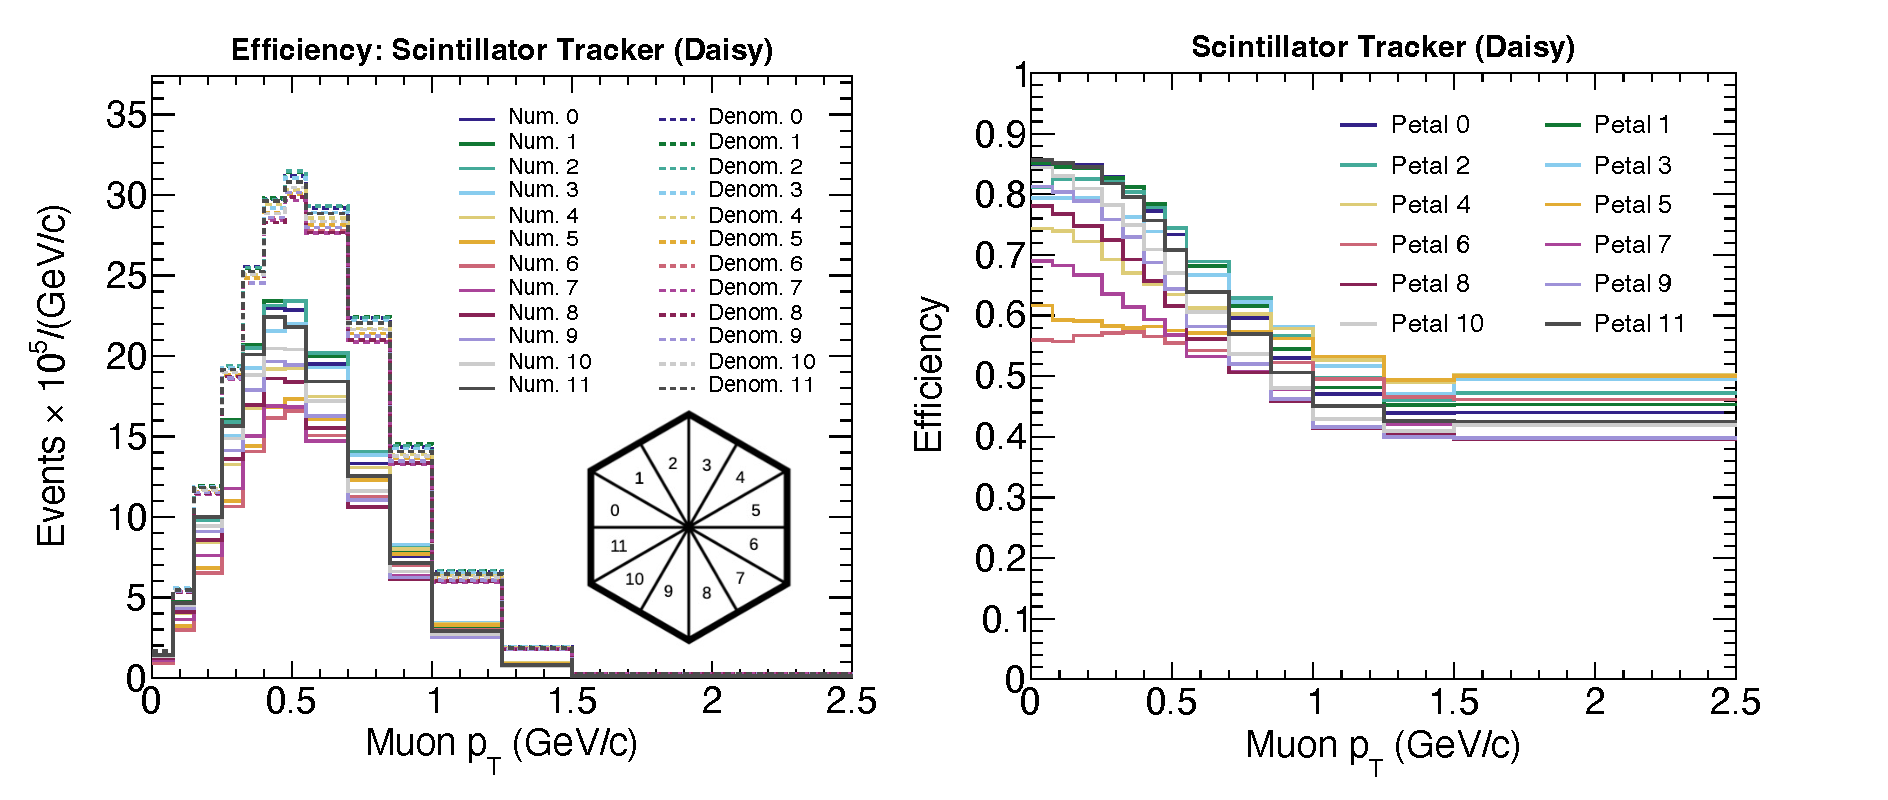
\includegraphics[width=1\textwidth]{07analysis1D/figures/efficiency_tracker_pT_daisy.pdf}}%
    \caption{Left:~Efficiency numerator and denominator for the scintillator tracker in `daisy petals' in antimuon $p_{\text{T}}$.~The hexagon insert illustrates petal positions looking downstream of the detector.~Right:~Efficiency distribution for the scintillator tracker in `daisy petals' in antimuon $p_{\text{T}}$. }
    %[short caption] {long caption}
    \label{fig:efficiency_tracker_pT_daisy}
\end{figure}


Finally, it is important to note that the scintillator tracker efficiency is also extracted in the `daisy petals', as illustrated in Figure~\ref{fig:efficiency_tracker_pT_daisy} for $p_{\text{T}}$. This extraction is essential for determining nuclear target-to-scintillator cross-section ratios using the matching flux technique discussed in Section~\ref{sec:nuclear_target_flux}. Similarly to the passive targets, the petals shadowing the MINOS coil have reduced efficiency at low $p_{\text{T}}$. All efficiency correction distributions for passive targets, scintillator tracker, and scintillator tracker divided in the `daisy petals' and their corresponding fractional uncertainties are included in Appendix~\ref{ch:appendix_efficiencyCorrection}.


\begin{comment}
After the efficiency correction, individual targets of the same material can be combined. In practice, this means adding up the efficiency-corrected histograms for targets 2,3 and 5 iron and 2-5 lead. Furthermore, the individual `daisy petals' of the scintillator tracker can be combined for cross-section ratios - a linear combination of the 

An example of the lead efficiency-corrected distribution, its fractional uncertainty and the scintillator tracker combined to match the individual targets is shown. The fractional error on the base scintillator tracker unfolded distributions is shown for comparison. 
\end{comment}

[Plots of efficiency-corrected distributions]

[For tracker cross-section used in cross-section ratios, this is where the individual distributions get combined]

\newpage
\section{Normalisation}

The final step in the calculation of the differential cross-section involves normalising the efficiency-corrected distribution according to the Equation~\ref{eq:xsec1D}.~First, each bin of the
efficiency-corrected distribution is divided by the number of scattering centres $T_{\text{nucleons}}$, i.e. the number of nucleons, within the fiducial volume available for an antineutrino to interact with in a given material.~Reporting the cross-section per nucleon ensures the result is independent of the detector's mass. The estimates of the number of nucleons in Table~\ref{table:normalisation} are derived from MINERvA's material assays~\cite{Aliaga_2014}. 

Furthermore, to report a differential cross-section, one must divide each bin $\alpha$ of the efficiency-corrected distribution by the integrated antineutrino flux prediction $\Phi$ and the corresponding bin width $\Delta x_{\alpha}$.~The antineutrino flux integral is calculated as a function of true antineutrino energy between 0--120~GeV using the flux simulation prediction outlined in Sections~\ref{sec:NuMI} and \ref{sec:fluxSimulation}.~The upper limit is determined by the 120~GeV/$c$ protons from which the NuMI antineutrino beam originates.~However, the contribution above 20~GeV is negligible as illustrated in Figure \ref{fig:antinu_fluxes} due to the muon energy cut discussed in Section~\ref{sec:eventSelection}. 

In line with the discussion in Section~\ref{sec:nuclear_target_flux}, Figure \ref{fig:antinu_fluxes} illustrates that antineutrino fluxes across different materials vary.~Consequently, the antineutrino flux integrals per protons on target (POT) are also shown to vary for different materials in Table~\ref{table:normalisation}. To eliminate the POT dependence, each flux integral in Table \ref{table:normalisation} is multiplied by the total data exposure of $1.12 \times 10^{21}$ POT in the cross-section extraction. A simple dimensional analysis shows that the differential cross-sections $\text{d}\sigma/\text{d}p_{T}$ and $\text{d}\sigma/\text{d}x$ can be reported in units of $10^{-39}/\text{cm}^{2}/\text{unit}/\text{nucleon}$, where `unit' represents the unit of the kinematic variable for which the differential cross-section was calculated.


%The flux normalisation also propagates the uncertainties associated with the flux, which are explained in Chapter~\ref{ch:systematics}.

%while accounting for the uncertainty associated with the target masses described in Chapter~\ref{ch:systematics}.
%N neutrons: mass * TargetProp::AtomsPerGram::C   * TargetProp::NeutronsPerAtom::C;

\begin{figure}[t!] 
    \centering
    {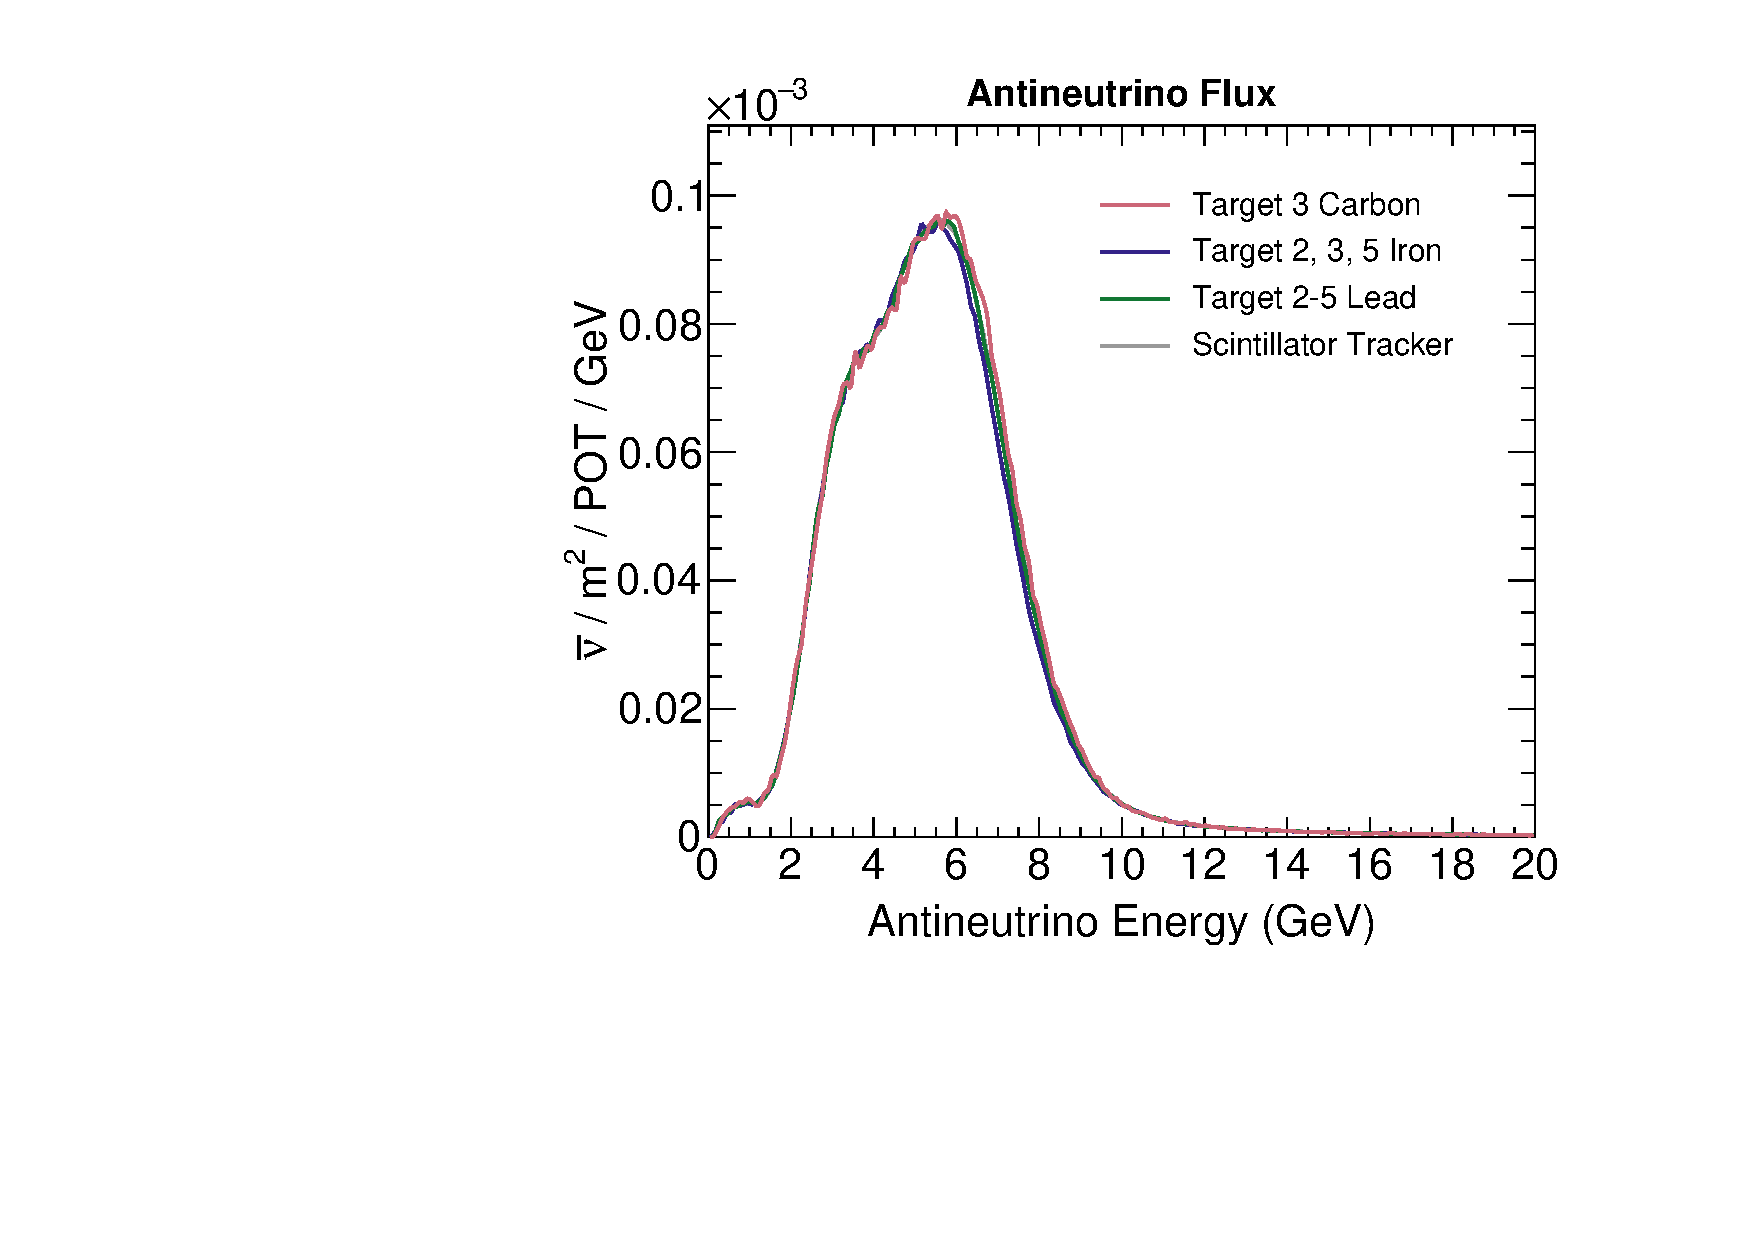
\includegraphics[width=1\textwidth]{07analysis1D/figures/antinu_flux.pdf}}%
    \caption{Antineutrino flux as a function of antineutrino energy between 0--20~GeV for carbon, iron, lead, and scintillator tracker. The contribution above 20~GeV is negligible.}
    %[short caption] {long caption}
    \label{fig:antinu_fluxes}
\end{figure}



\begin{table}[b!]
    \centering

    \begin{tabular}{c c c}
    \hline \\ [-1.5 ex]
    Material & $\Phi$ $(\bar{\nu}_{\mu} \times 10^{-8}/\text{cm}^{2}/\text{POT})$ & $T_{\text{nucleons}}$ $(\times 10^{28})$ \\ [0.5ex] % inserts table %heading
    \hline\hline
    Carbon & 4.853 & 9.598 \\ %9.59755e+28 \\
    %\hline
    Iron & 4.676 & 37.841 \\ % 3.78413e+29 \\
    %\hline
    Lead & 4.763 & 42.768 \\%4.27675e+29 \\
    %\hline
    Scintillator & 4.774 & 323.478 \\ %3.23478e+30 \\
    \hline
    \end{tabular}

    \caption{Cross-section normalisation factors for the passive target region and the scintillator tracker.}
    \label{table:normalisation}
\end{table}


\section{Cross-section distributions}
\section{Cross-section ratios}
\section{Validation}



\clearpage
\thispagestyle{empty}
\hfill
\clearpage
\chapter{Systematic uncertainties}

\label{ch:systematics}

Every cross-section measurement, such as the one presented here, inherently carries uncertainties crucial for understanding the reliability and precision of the reported result. These uncertainties can be divided into two categories: statistical and systematic.

The statistical uncertainty essentially accounts for the fact that a cross-section measurement is a counting experiment with a finite number of counts. Specifically, this work involves counting antineutrino interactions in bins of $p_{\text{T}}$ and Bjorken~$x$. Each count, i.e. the observed interaction, originates from an underlying Poisson probability distribution. Therefore, the statistical uncertainty of a given bin with $N$ events corresponds to $\sqrt{N}$. 
% p24: https://indico.cern.ch/category/6015/attachments/192/629/Statistics_introduction.pdf
%observed number of events will be Poisson distributed a the normal approximation to the Poisson distribution. 
%Note that the statistical uncertainty of the unfolded distribution is corrected to account for the finite statistics of the unfolding matrix as described in Section~\ref{sec:migration_unfolding}. 

In contrast, systematic uncertainties in this measurement describe the accuracy with which the cross-section can be measured, taking into account the limitations of the MINERvA and MINOS detectors and reconstruction, as well as the understanding of the incident antineutrino beam and its interactions with nuclei. MINERvA uses the underlying simulation to estimate systematic uncertainties in reported cross-section results via the multiverse method \cite{MAT_Messerly_2021}, which has already been mentioned in Chapters~\ref{ch:minerva} and \ref{ch:dataAsimulation} with respect to flux modelling. The simulation with nominal values for all parameters, as described in Chapter~\ref{ch:dataAsimulation}, is referred to as the central value~(CV). A~systematic universe is then a simulation sample in which one or more input parameters are varied within their associated uncertainties. 

As discussed, the antineutrino flux, due to its complex modelling, necessitates the multiverse approach to allow simultaneous variations of multiple parameters. However, most systematic uncertainties have relatively simple underlying models and are typically evaluated by considering two universes where a parameter is shifted by $\pm 1 \sigma$, with $\sigma$ representing the parameter's uncertainty. The magnitude of the uncertainty in each bin is then given by the spread of these two universes, i.e. the average difference between each universe and the CV in that bin. All systematic universes are propagated throughout the analysis.

\begin{figure}[t!]%
    \centering
    \vspace{-5pt}
   {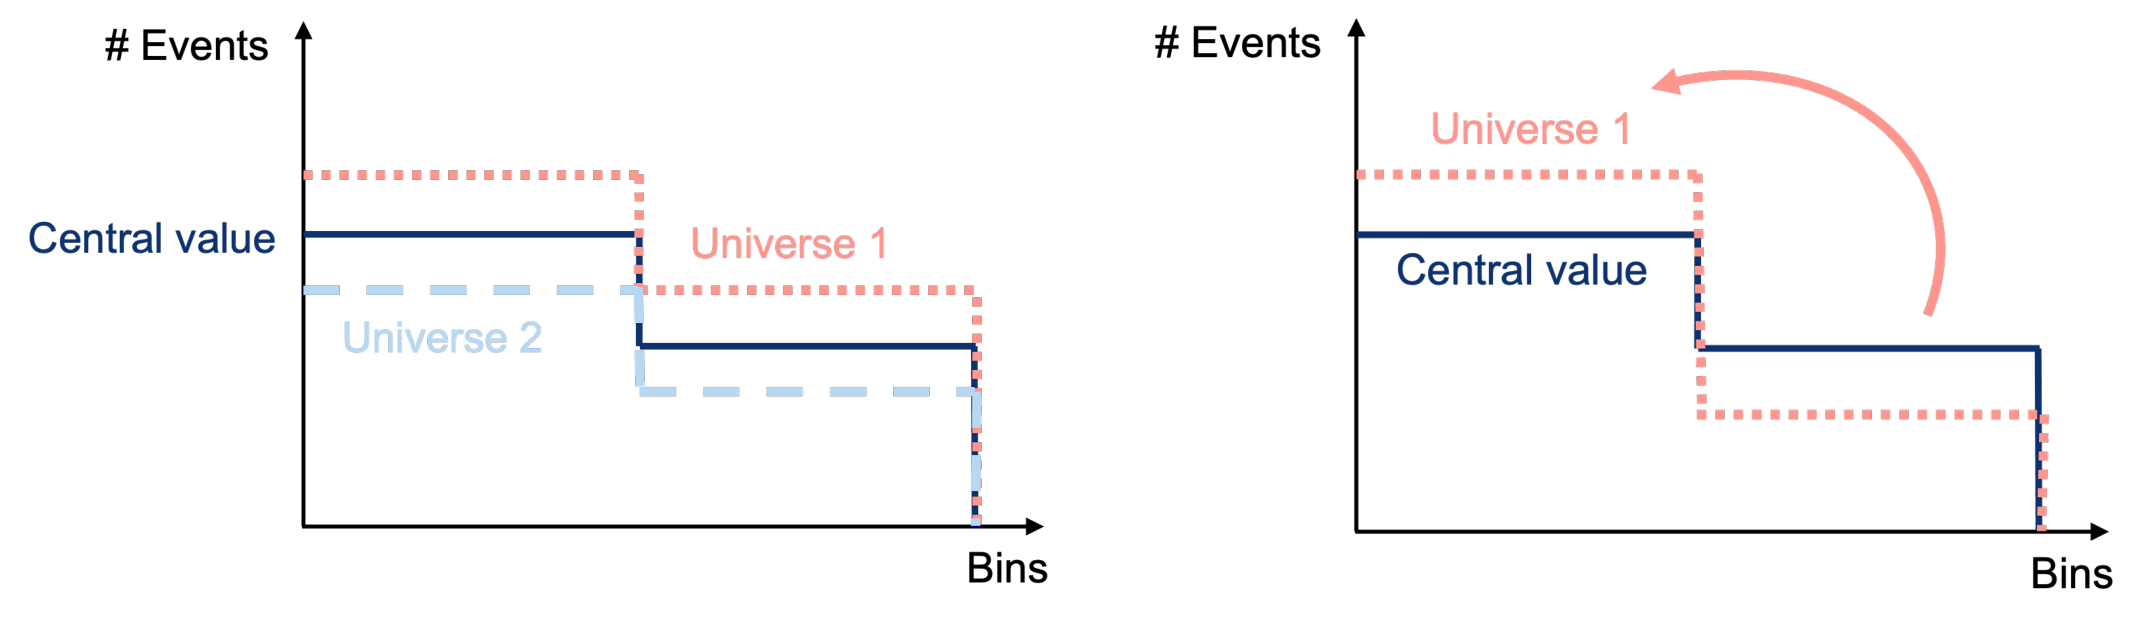
\includegraphics[width=0.9\textwidth]{08systematics/figures/systematicShifts.pdf} }%
    \caption{Illustration of two different effects a systematic universe can have on an event---a normalisation-like shift (left) and a bin-by-bin shift (right). }%
    \label{fig:sysShifts}
\end{figure}

Conceptually, there are two effects a systematic universe can have on an event: a~normalisation-like shift and a bin-by-bin shift, as illustrated in Figure~\ref{fig:sysShifts}. Normalisation-like shifts represent uncertainties that affect the weight of an event in a given bin, such as those from interaction models. In contrast, bin-by-bin uncertainties impact the kinematic variables, causing bin-to-bin migration, and represent most detector systematics. 

Figure~\ref{fig:mcSimulationFracUnc_t5lead_pTx} shows an example of the fractional uncertainty\footnote{Fractional uncertainty error band represents the uncertainties relative to the CV, i.e.~uncertainty/CV.} on the simulation for target~5 lead both in $p_{\text{T}}$ and Bjorken~$x$ at the event rate level. Appendix~\ref{ch:appendix_sysUncertainties} includes the corresponding breakdown of uncertainties for the scintillator tracker. Related sources of uncertainties are grouped together in one error band and will be discussed individually later with respect to the reported cross-section. The individual systematic errors within these groups are constructed by extracting the square root of diagonal entries (variances) of their corresponding covariance matrices. 

An element of the covariance matrix relating two bins $i$~and $j$ can be calculated as
\vspace{-7pt}
\begin{equation}
    \label{eq:covariance}
    %\vspace{-10pt}
    \text{cov}_{ij} = \frac{1}{N-1}\sum_{n=1}^{N}(x_{n, i} - \bar{x}_i)(x_{n, j} - \bar{x}_j)
    \hspace{3pt},
    \vspace{5pt}
    %\text{cov}_{ij} = \frac{\sum_{n=1}^{N} (x_{n, i} - \bar{x}_i)(x_{n, j} - \bar{x}_j)w_n}{\sum_{n=1}^{N} w_n}\hspace{3pt},
\end{equation}
where $N$ represents the total number of universes, $x_n$ is the bin content of a given bin in the universe $n$, and $\bar{x}$ is the mean of all the universes in that bin.  Note that the off-diagonal terms of the covariance matrix are retained and used in comparisons with various other antineutrino generators with different interaction models in Chapter~\ref{ch:results} to account for bin-to-bin correlations.~The error band grouping related sources of uncertainty in each bin is then calculated as the square root of the sum of the diagonal elements of all relevant individual covariance matrices. The total error band is calculated the same way but also includes the statistical uncertainty.

%In this way, the variance of each bin is added in quadrature as expected for uncorrelated uncertainties.

\begin{figure}[t!]%
    \vspace{-7pt}
    \centering
   {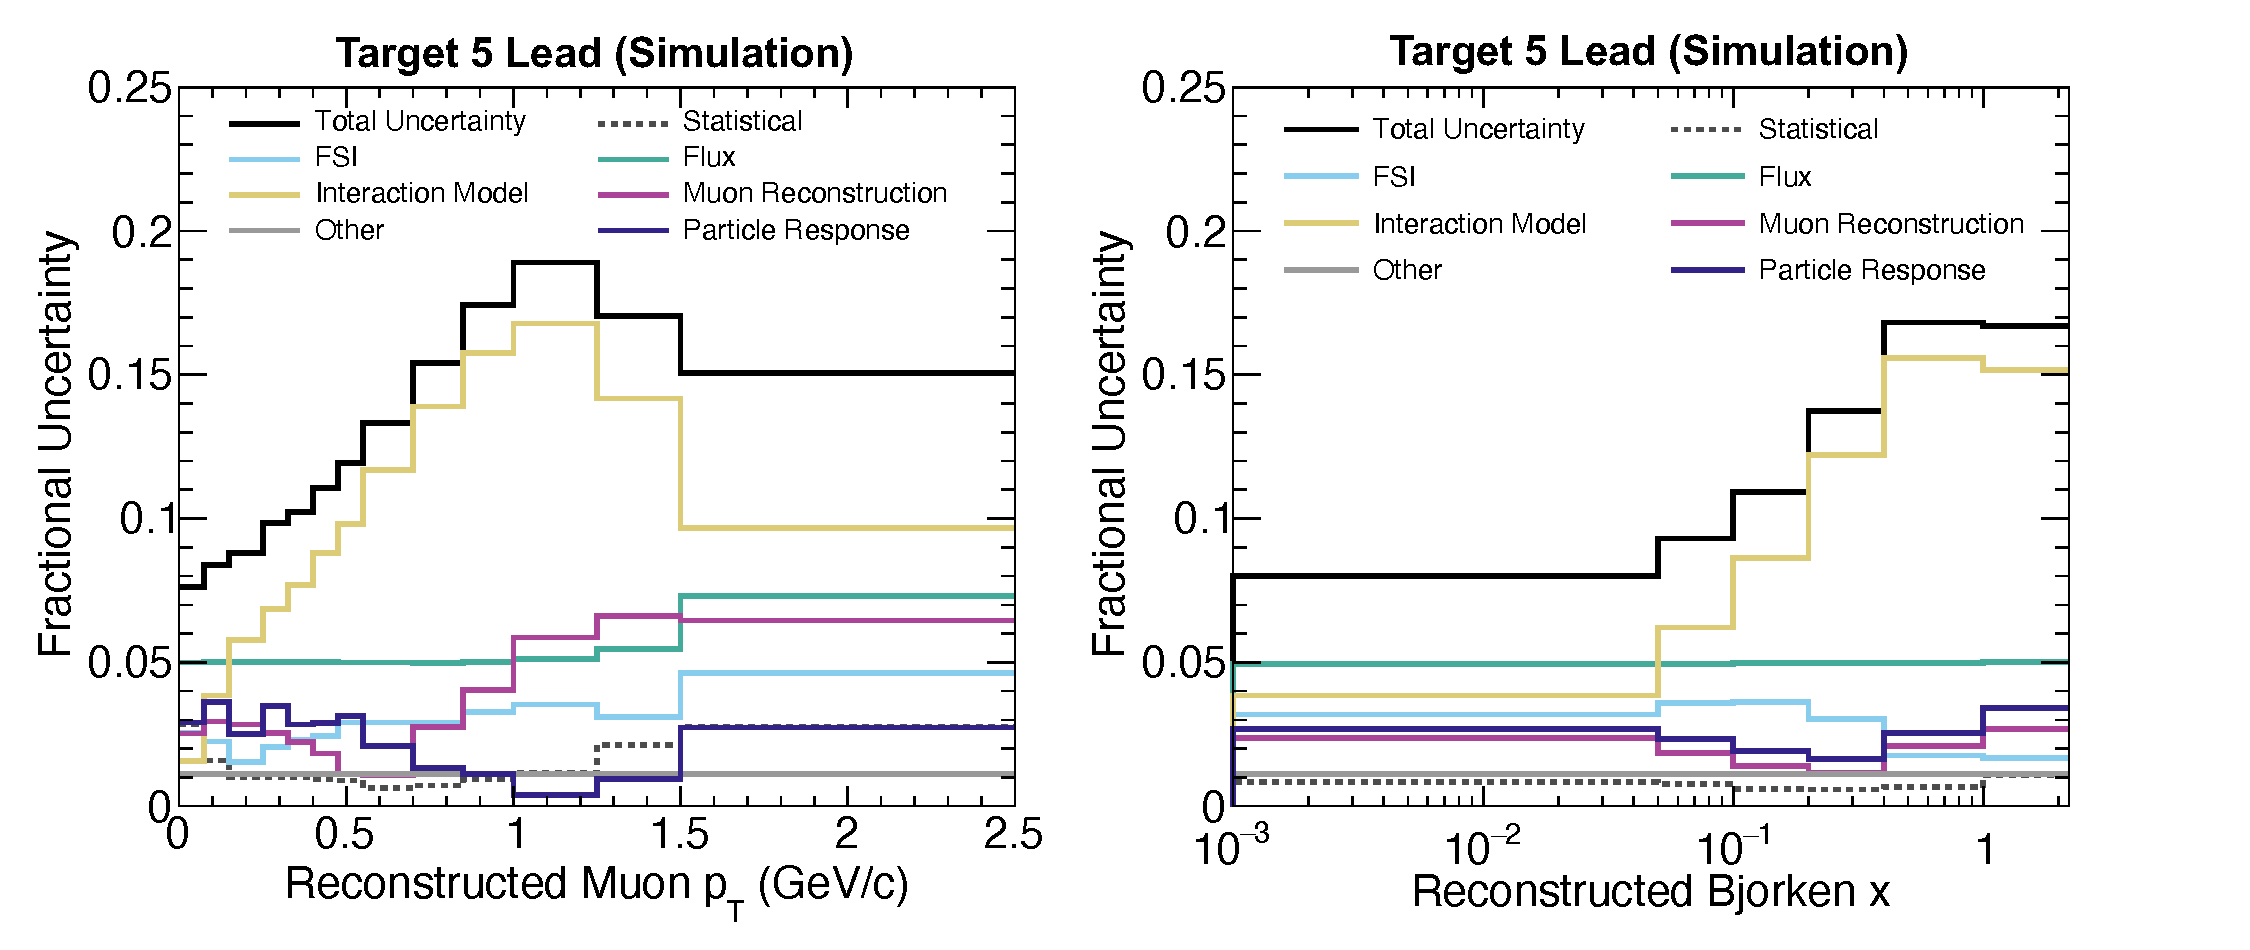
\includegraphics[width=1\textwidth]{08systematics/figures/mcSimulationFracUnc_t5lead_pTx.pdf} }%
    \caption{Fractional uncertainty breakdown for the simulated event rate in both $p_{\text{T}}$~(left) and Bjorken~$x$ (right) in target 5 lead.}%
    \label{fig:mcSimulationFracUnc_t5lead_pTx}
\end{figure}

The multiverse method enables independent cross-section analysis in each universe. While the systematic uncertainty is reported on the simulation at the event rate level, in the final cross-section result, MINERvA reports the systematic uncertainty on the data. This is due to the cross-section extraction steps outlined in Equation~\ref{eq:xsec1D}, i.e. background subtraction, unfolding, efficiency correction, and normalisation, where information from the simulation introduces systematic uncertainty to the data.

The (data) cross-section uncertainty for the differential cross-section on lead in $p_{\text{T}}$ and Bjorken~$x$ is presented in Figure~\ref{fig:crossSectionFracUnc_lead_pTx}. The individual error band categories are discussed in detail in the following sections.\enlargethispage{1\baselineskip} However, it is important to note that Figure~\ref{fig:crossSectionFracUnc_lead_pTx} illustrates a general trend observed across various materials for the last $p_{\text{T}}$ and Bjorken~$x$ bin. Specifically, the last $p_{\text{T}}$ bin, extending to the edge of the angular acceptance, leads to statistical fluctuations in the associated systematic uncertainty.~On the other hand, the last Bjorken~$x$ bin is significantly influenced by interaction model uncertainties since the simulation doesn't directly model this region at the nucleon level, as discussed previously. In the kinematic distributions (as opposed to fractional uncertainty plots), where the data carries the systematic uncertainty, the data points are represented with inner and outer error bars, corresponding to the statistical and total (statistical + systematic) uncertainty, respectively.



\begin{figure}[t!]%
    \centering
    \vspace{-7pt}
   {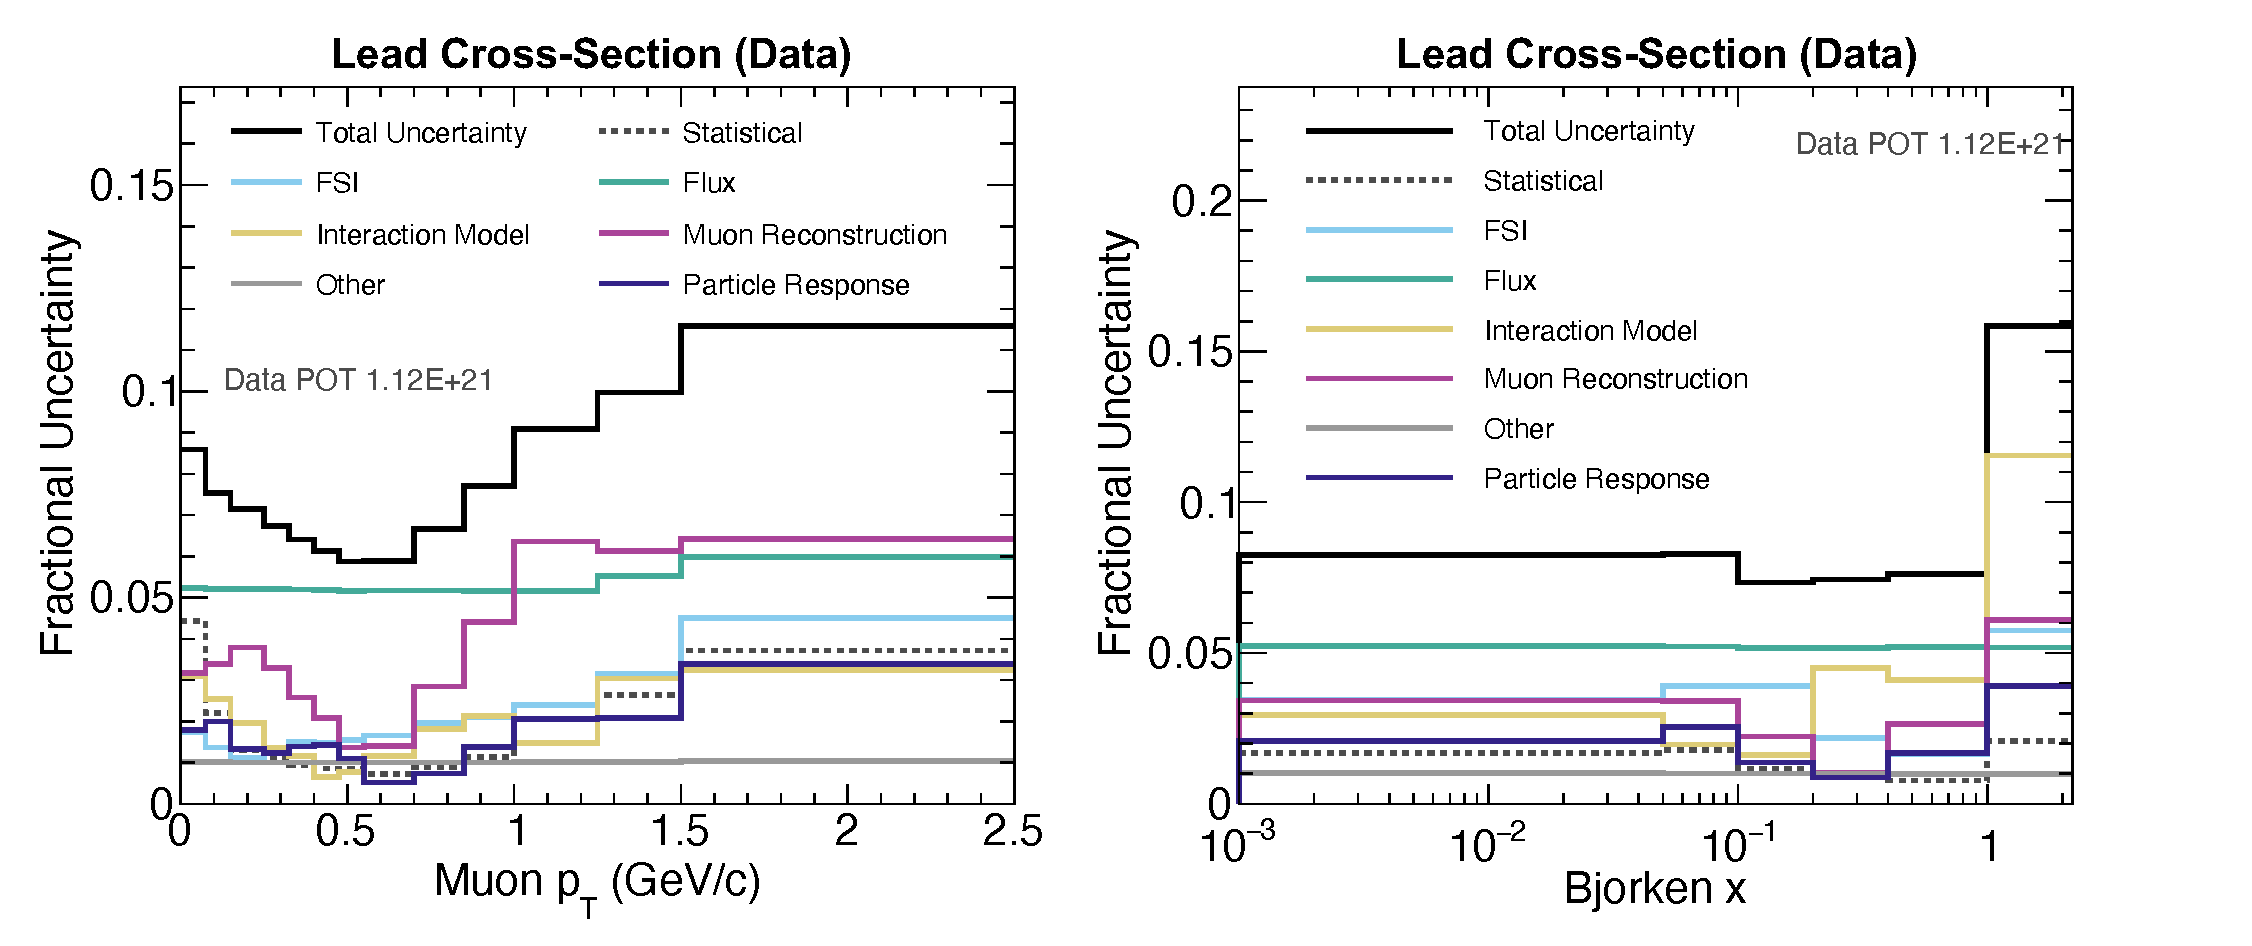
\includegraphics[width=1\textwidth]{08systematics/figures/crossSectionFracUnc_lead_pTx.pdf} }%
    \caption{Breakdown of the fractional uncertainties propagated to the lead differential cross-section in data in both $p_{\text{T}}$~(left) and Bjorken $x$ (right).}%
    \label{fig:crossSectionFracUnc_lead_pTx}
\end{figure}

\section{Flux}

Similarly to other cross-section analyses, the flux uncertainty represents the leading systematic uncertainty in this measurement as well\footnote{One of the primary reasons for reporting cross-section ratios is to cancel out the dominant flux uncertainty.}. The flux modelling and its associated uncertainties have been discussed in detail in Chapters~\ref{ch:minerva} and \ref{ch:dataAsimulation}. MINERvA's PPFX package \cite{AliagaSoplin:2016shs, Aliaga_2014} evaluates the flux uncertainty in 1000 systematic universes, where each universe represents an ensemble of systematic variations of underlying beam-focusing and hadron production parameters to account for their non-trivial correlations resulting from the fits described in Subsection~\ref{subsec:numiSim}.

In addition, MINERvA applies an \textit{in-situ} constraint combining measurements of (anti)neutrino-electron scattering and IMD \cite{Zazueta2023_PhysRevD.107.012001}, which significantly reduces the flux uncertainty in the antineutrino-dominated beam to about 5\% as evident from Figure~\ref{fig:crossSectionFracUnc_lead_pTx}. The \textit{in-situ} constraint assigns weights to the individual flux universes, with some being weighted much more than others, allowing for their ordering in terms of significance. Previous MINERvA studies have shown that, in most cases, the most significant 100 universes adequately sample the range of systematic variations \cite{fluxReorderingRobFine}. This allows for a reduction in computational power when evaluating the flux uncertainty at the cross-section measurement level, and is therefore used in this analysis. Note that the flux uncertainty in both $p_{\text{T}}$ and Bjorken~$x$, as shown in Figure~\ref{fig:crossSectionFracUnc_lead_pTx}, is flat since the cross-sections are differential.


\section{Antimuon reconstruction}

\begin{figure}[b!]%
    \centering
   {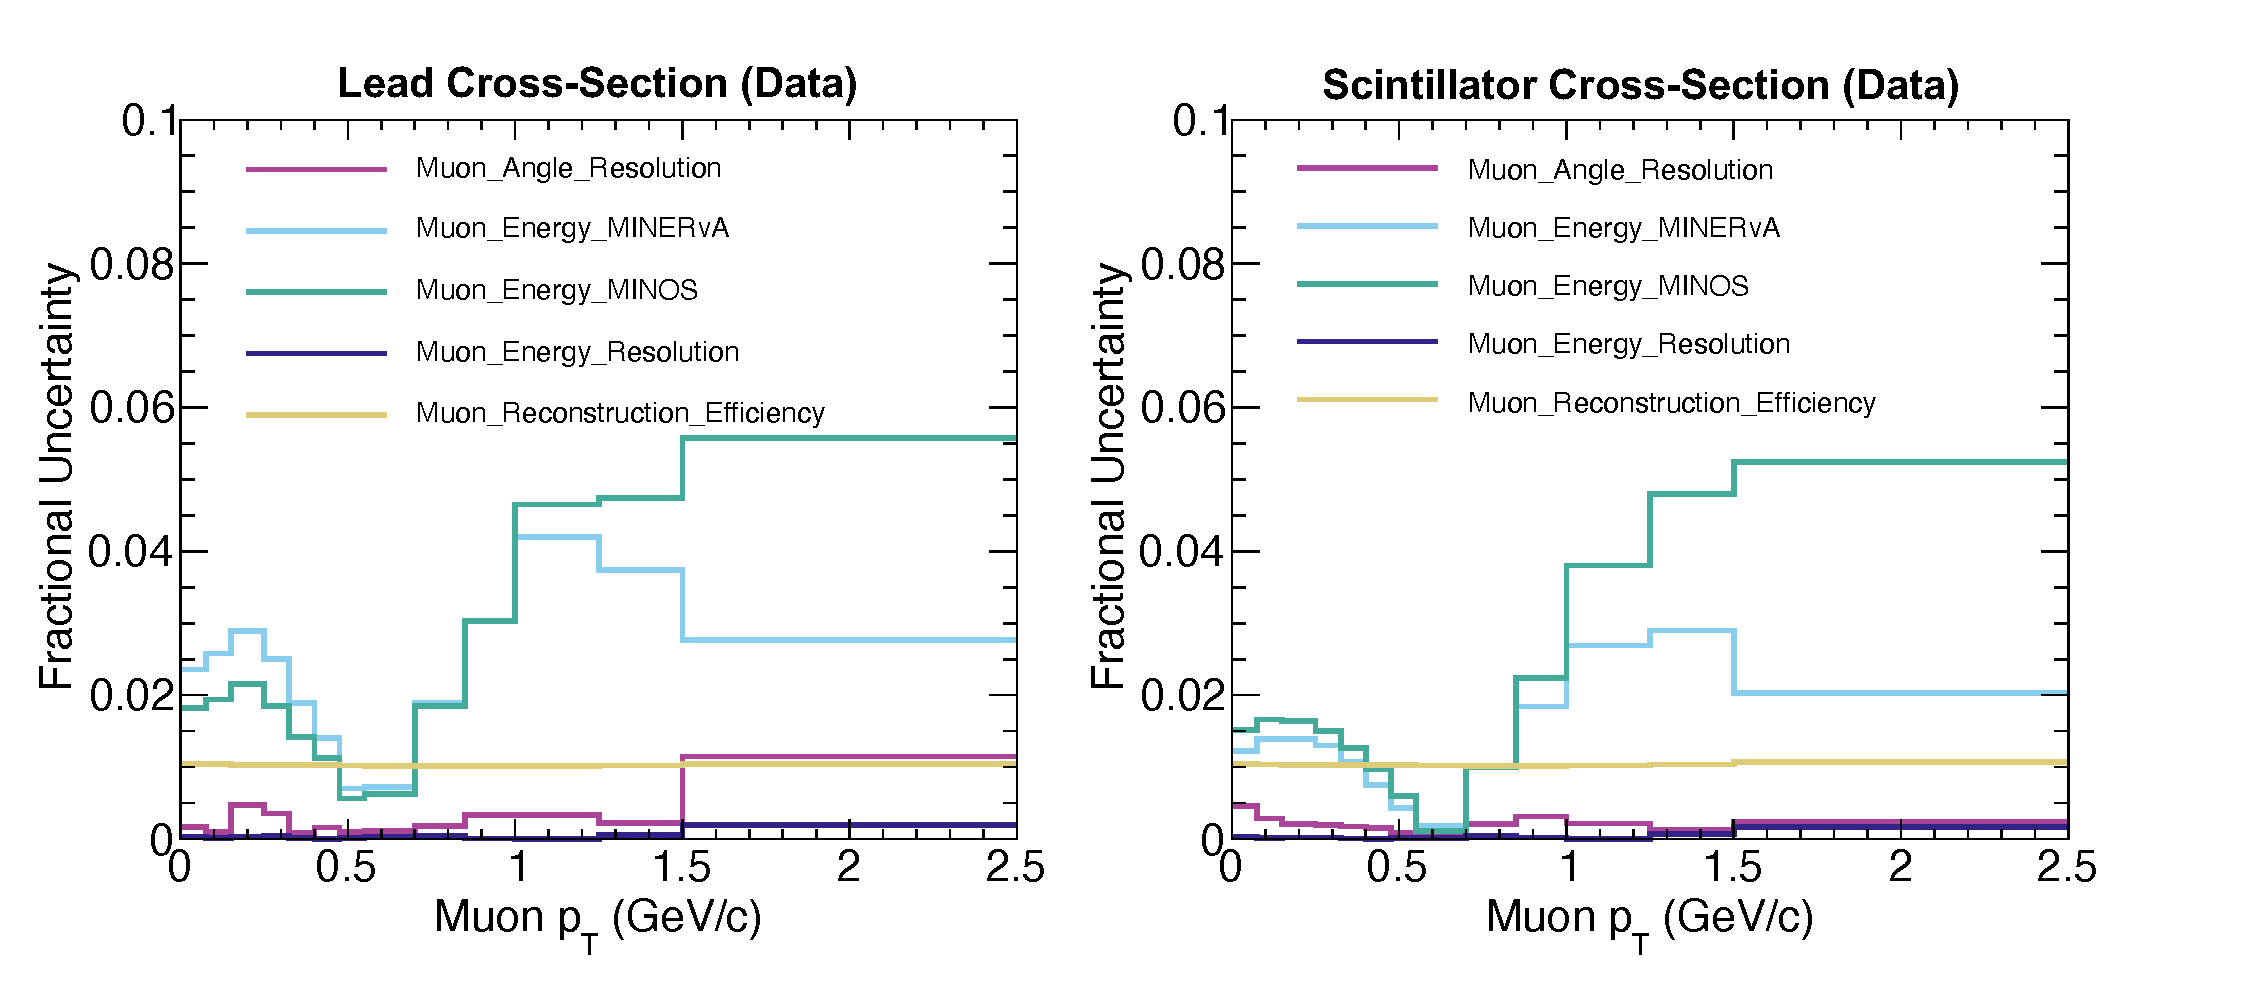
\includegraphics[width=1\textwidth]{08systematics/figures/muonReco_leadTracker_pT.pdf} }%
    \caption{Breakdown of various sources of uncertainty in the `Muon Reconstruction' error band in the lead (left) and scintillator (right) differential cross-section in data in $p_{\text{T}}$.}%
    \label{fig:muonReco_leadTracker_pT}
\end{figure}

The uncertainty related to antimuon reconstruction is the second-largest (third-largest) uncertainty in the  $p_{\text{T}}$ (Bjorken $x$) differential cross-section.\enlargethispage{1.5\baselineskip} Figure~\ref{fig:muonReco_leadTracker_pT} shows the error band broken down into the various sources of uncertainties for both lead and scintillator cross-sections in $p_{\text{T}}$, while the corresponding breakdown for Bjorken~$x$ is provided in Appendix~\ref{ch:appendix_sysUncertainties}. The $p_{\text{T}}$ breakdown is dominated by the uncertainty on the antimuon energy reconstruction in the MINERvA detector and MINOS spectrometer. The MINERvA uncertainty combines the 40~MeV (30~MeV) uncertainty on the energy deposits per unit length and the  17~MeV (11~MeV) material assay uncertainty for the passive target region (active tracker region)~\cite{Tice_PhysRevLett.112.231801}. The MINOS uncertainty comes from the~0.98\% uncertainty on antimuons reconstructed by range, and the~2.1\%~(3.2\%) uncertainty on antimuons with momenta above (below) 1~GeV reconstructed by curvature~\cite{Aliaga_2014}, as described in Chapter~\ref{ch:Reconstruction}.
% there is also material assay uncertainty 11 MeV shift vs 17 MeV

The flat reconstruction efficiency uncertainty band represents the uncertainty on the tracking efficiency of the MINOS spectrometer stemming from the antimuon energy- and beam intensity-dependent correction applied to the simulation to match the data, also discussed in Chapter~\ref{ch:Reconstruction}. The antimuon angle uncertainty encompasses the 2\% uncertainty on the reconstructed antimuon angle~\cite{Ziemer:2012ota}, and the 1~mrad antimuon angle bias coming from the uncertainty on the incoming antineutrino beam angle~\cite{Valencia-Rodriguez:2016vkf}. Finally, the uncertainty in antimuon energy resolution corresponds to 0.4\%~\cite{Bashyal:2021tzd} and quantifies any remaining antimuon energy resolution differences between the data and the simulation.


% muon track uncertainty https://lss.fnal.gov/archive/thesis/2000/fermilab-thesis-2012-62.pdf
% beam angle thing: https://www.osti.gov/biblio/1341804
% muon energy resoltion - I guess bercelie? or Bashyal?


\section{Interaction model}
% summary table for GENIE uncertainties:
% https://minerva-docdb.fnal.gov/cgi-bin/sso/RetrieveFile?docid=7451&filename=ReweightingSystematics.pdf&version=2

\begin{figure}[t!]%
    \centering
    \vspace{-7pt}
   {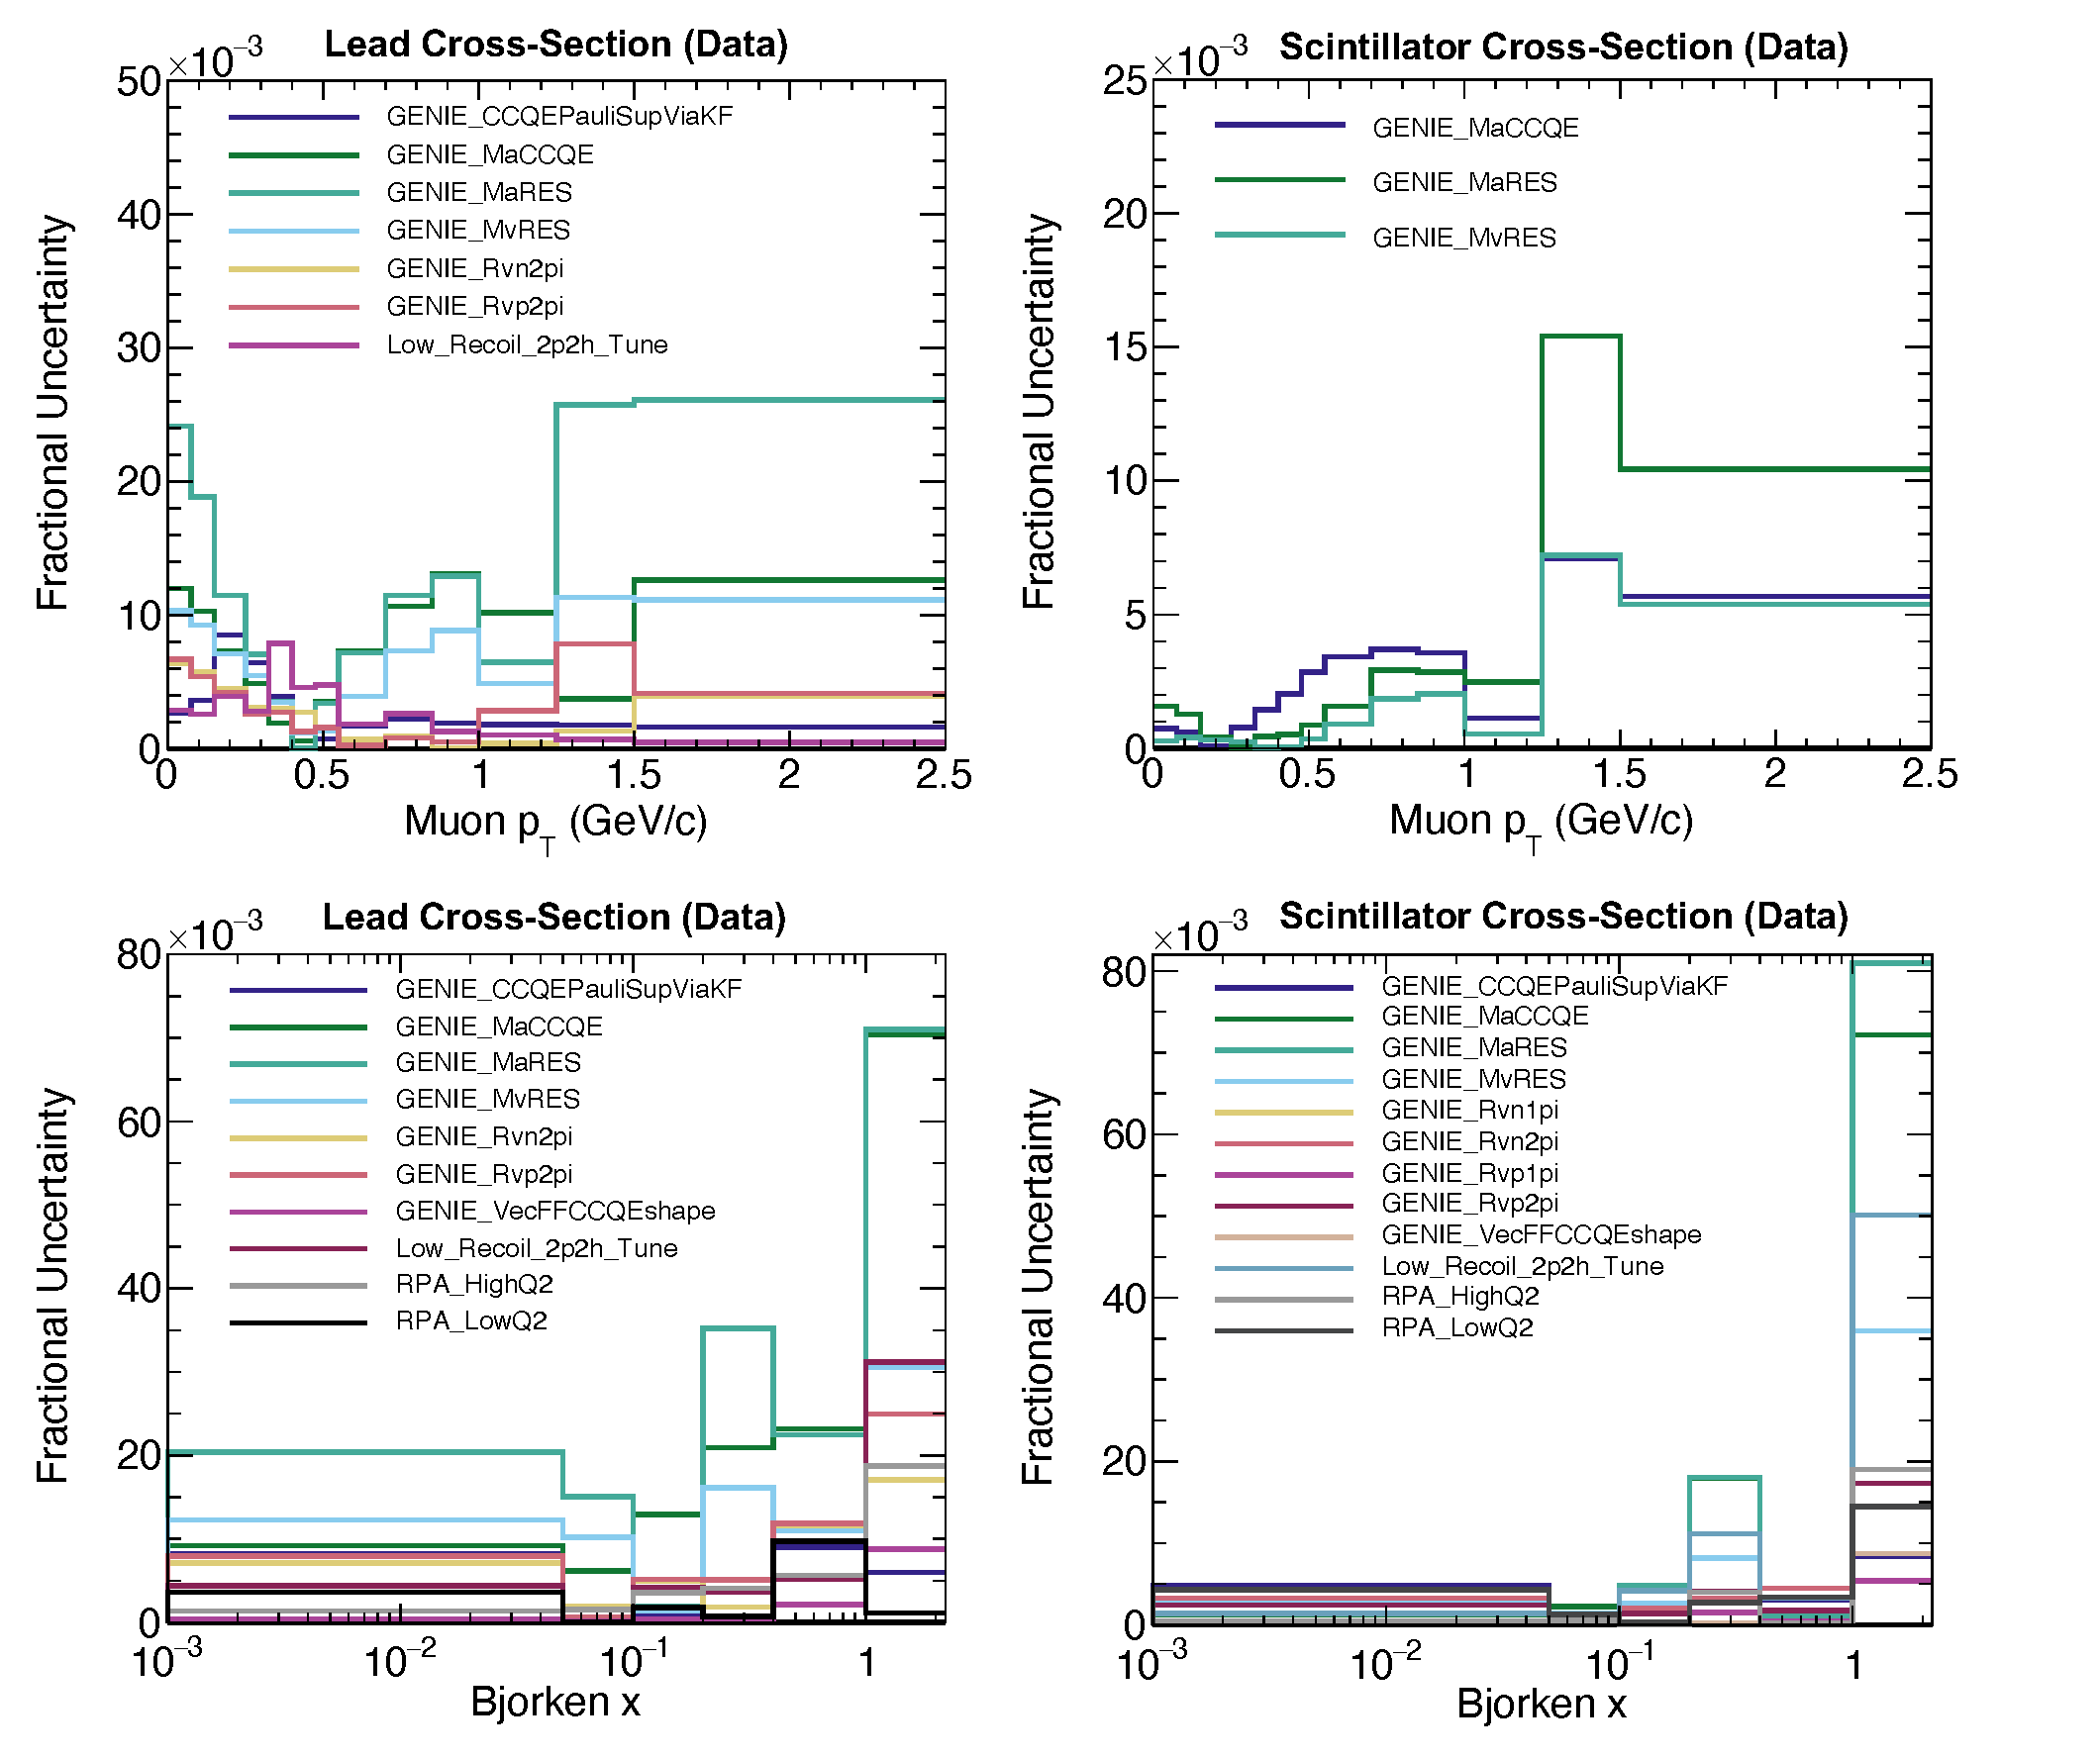
\includegraphics[width=1\textwidth]{08systematics/figures/intModel_t5Tracker_pTx.pdf} }%
    \caption{Breakdown of various sources of uncertainty in the `Interaction Model' error band of the differential cross-section in data, both in $p_{\text{T}}$ (top) and Bjorken $x$ (bottom) for lead (left panel) and scintillator (right panel), with contributions exceeding 0.5\%. Note the dominant contribution from the uncertainty on the resonant pion production axial mass.}%
    \label{fig:intModel_t5Tracker_pTx}
\end{figure}

The initial state and initial interaction models used in the simulation, described in detail in Chapter~\ref{ch:dataAsimulation}, have several parameters that adjust the probability of an interaction process occurring. The underlying uncertainties associated with these parameters in GENIE~\cite{genie_ANDREOPOULOS201087,genie_andreopoulos2015}, derived from previous experimental measurements, enable the construction of alternative universes to evaluate corresponding systematic uncertainties in the measurement. Some of these default uncertainties are constrained using MINERvA's measurements and re-analyses of other data. There are also additional uncertainties related to the previously discussed RPA and 2p2h implementations. All these uncertainties are combined in the `Interaction Model' error band, as shown in Figures~\ref{fig:mcSimulationFracUnc_t5lead_pTx} and~\ref{fig:crossSectionFracUnc_lead_pTx}.\enlargethispage{1\baselineskip}
% uncertainties on various parameters: GENIE source code
% https://github.com/GENIE-MC/Generator/blob/R-2_12_6/src/ReWeight
% https://indico.fnal.gov/event/11610/contributions/9102/

% info from: https://minerva-docdb.fnal.gov/cgi-bin/sso/RetrieveFile?docid=7451&filename=ReweightingSystematics.pdf&version=2
% https://github.com/MinervaExpt/MAT-MINERvA/blob/main/utilities/NSFDefaults.h
% Bercellie thesis and Rob Fine thesis
\begin{table}[t!]
    \centering
    \small
    \begin{tabularx}{1.0\textwidth}{c c L}
    \hline \\ [-1.5 ex]
    Error band & 1$\sigma$ & Description\\ [0.5ex] % inserts table %heading
    \hline
    \hline \\ [-2ex]
    CCQEPauliSupViaKF & $\pm30$\% & Modifies Pauli blocking at low $Q^2$ by adjusting momentum cutoff \\
    MaCCQE & +25\%/-15\% & CCQE axial mass (0.99 GeV/$c^2$) in the Llewellyn-Smith cross-section (shape and normalisation) \\
    MaRES & $\pm0.05$ GeV/$c^2$ & RES axial mass (0.94 GeV/$c^2$) in the Rein-Sehgal cross-section (shape and normalisation) \\
    MvRES & $\pm3$\% & RES vector mass (0.84 GeV/$c^2$) in Rein-Sehgal cross-section (shape and normalisation) \\
    Rvn1pi & $\pm4$\% & Strength of CC and NC 1$\pi$ production from non-resonant (Bodek-Yang) $\nu n$/$\bar{\nu}p$ interactions  \\
    Rvn2pi & $\pm50$\% & Strength of CC and NC 2$\pi$ production from non-resonant (Bodek-Yang) $\nu n$/$\bar{\nu}p$ interactions \\
    Rvp1pi & $\pm4$\% & Strength of CC and NC 1$\pi$ production from non-resonant (Bodek-Yang) $\nu p$/$\bar{\nu}n$ interactions \\
    Rvp2pi & $\pm50$\% & Strength of CC and NC 2$\pi$ production from non-resonant (Bodek-Yang) $\nu p$/$\bar{\nu}n$ interactions \\
    VecFFCCQEshape & BBBA~$\rightarrow$~dipole & CCQE vector form factor model change from BBBA to dipole (shape) \\
    \hline
    \end{tabularx}

    \caption{Description of various sources of uncertainty in the `Interaction Model' error band from Figure~\ref{fig:intModel_t5Tracker_pTx} with their corresponding 1$\sigma$ shifts.}
    \label{table:intModelUnc}
\end{table}

Figure~\ref{fig:intModel_t5Tracker_pTx} shows the uncertainties that contribute more than 0.5\% to the `Interaction Model' uncertainty band in the $p_{\text{T}}$ and Bjorken~$x$ differential cross-section in both lead and scintillator. A close-up of the scintillator breakdown in Bjorken~$x$ for the $x<1$ region is provided in Appendix~\ref{ch:appendix_sysUncertainties}. Overall, the error band is dominated by the resonant pion production axial mass uncertainty, which is expected given that resonant pion production is the dominant interaction channel in this analysis.~Additional notable contributions come from the uncertainty on the vector mass in resonant pion production and the axial mass in quasi-elastic scattering. All of these govern the cross-section shape and normalisation of their respective processes. Table~\ref{table:intModelUnc} lists and describes all GENIE parameter uncertainties contributing more than 0.5\%. Note that in comparison to the nominal uncertainties in GENIE, the uncertainty on $M_A^{\text{RES}}$ is constrained from the nominal 20\% to about~5\% by the reanalysis of the ANL/BNL deuterium bubble chamber measurements of single pion production~\cite{pion_Rodrigues_2016}, mentioned in Chapter~\ref{ch:dataAsimulation}. In addition, the uncertainties on the single-pion non-resonant production parameters are constrained from 50\% to 4\% using the same reanalysis. Fits~\cite{PhysRevD.74.014009} to pion production in electron-nucleon scattering~\cite{Tiator_2004} are also used to reduce the uncertainty on $M_V^{\text{RES}}$ from 10\% to 3\%.
% doc-db for vector mass uncertainty: https://minerva-docdb.fnal.gov/cgi-bin/sso/ShowDocument?docid=11567
% axial mass norminal uncertainty 20% of 

Furthermore, the uncertainty associated with the 2p2h model used in the MINERvA simulation, as described in Section~\ref{subsec:2p2h}, is assessed by varying the composition of correlated pairs of nucleons. This variation extends to the extremes of either exclusively proton-proton (neutron-neutron) pairs or exclusively neutron-proton pairs involved in the 2p2h process to construct the alternative universes~\cite{Gran2018_PhysRevLett.120.221805}. The RPA uncertainty is evaluated similarly by varying its implementation in the universes separately for the low-momentum and high-momentum transfer regions.\enlargethispage{1\baselineskip} The former comes from the comparisons against data for muon capture at low-momentum transfer, while the latter stems from the differences between the relativistic (implemented in the simulation CV) and the non-relativistic RPA calculation at high-momentum transfer~\cite{gran2017model}.

% 60% relativistic vs non-relativistic in high momentum - non-relativistic is higher
% data-driven  - 25\% normalisation difference

\section{FSI}
% FSI uncertainties description https://minerva-docdb.fnal.gov/cgi-bin/sso/ShowDocument?docid=7451
\begin{figure}[b!]%
    \vspace{-7pt}
    \centering
   {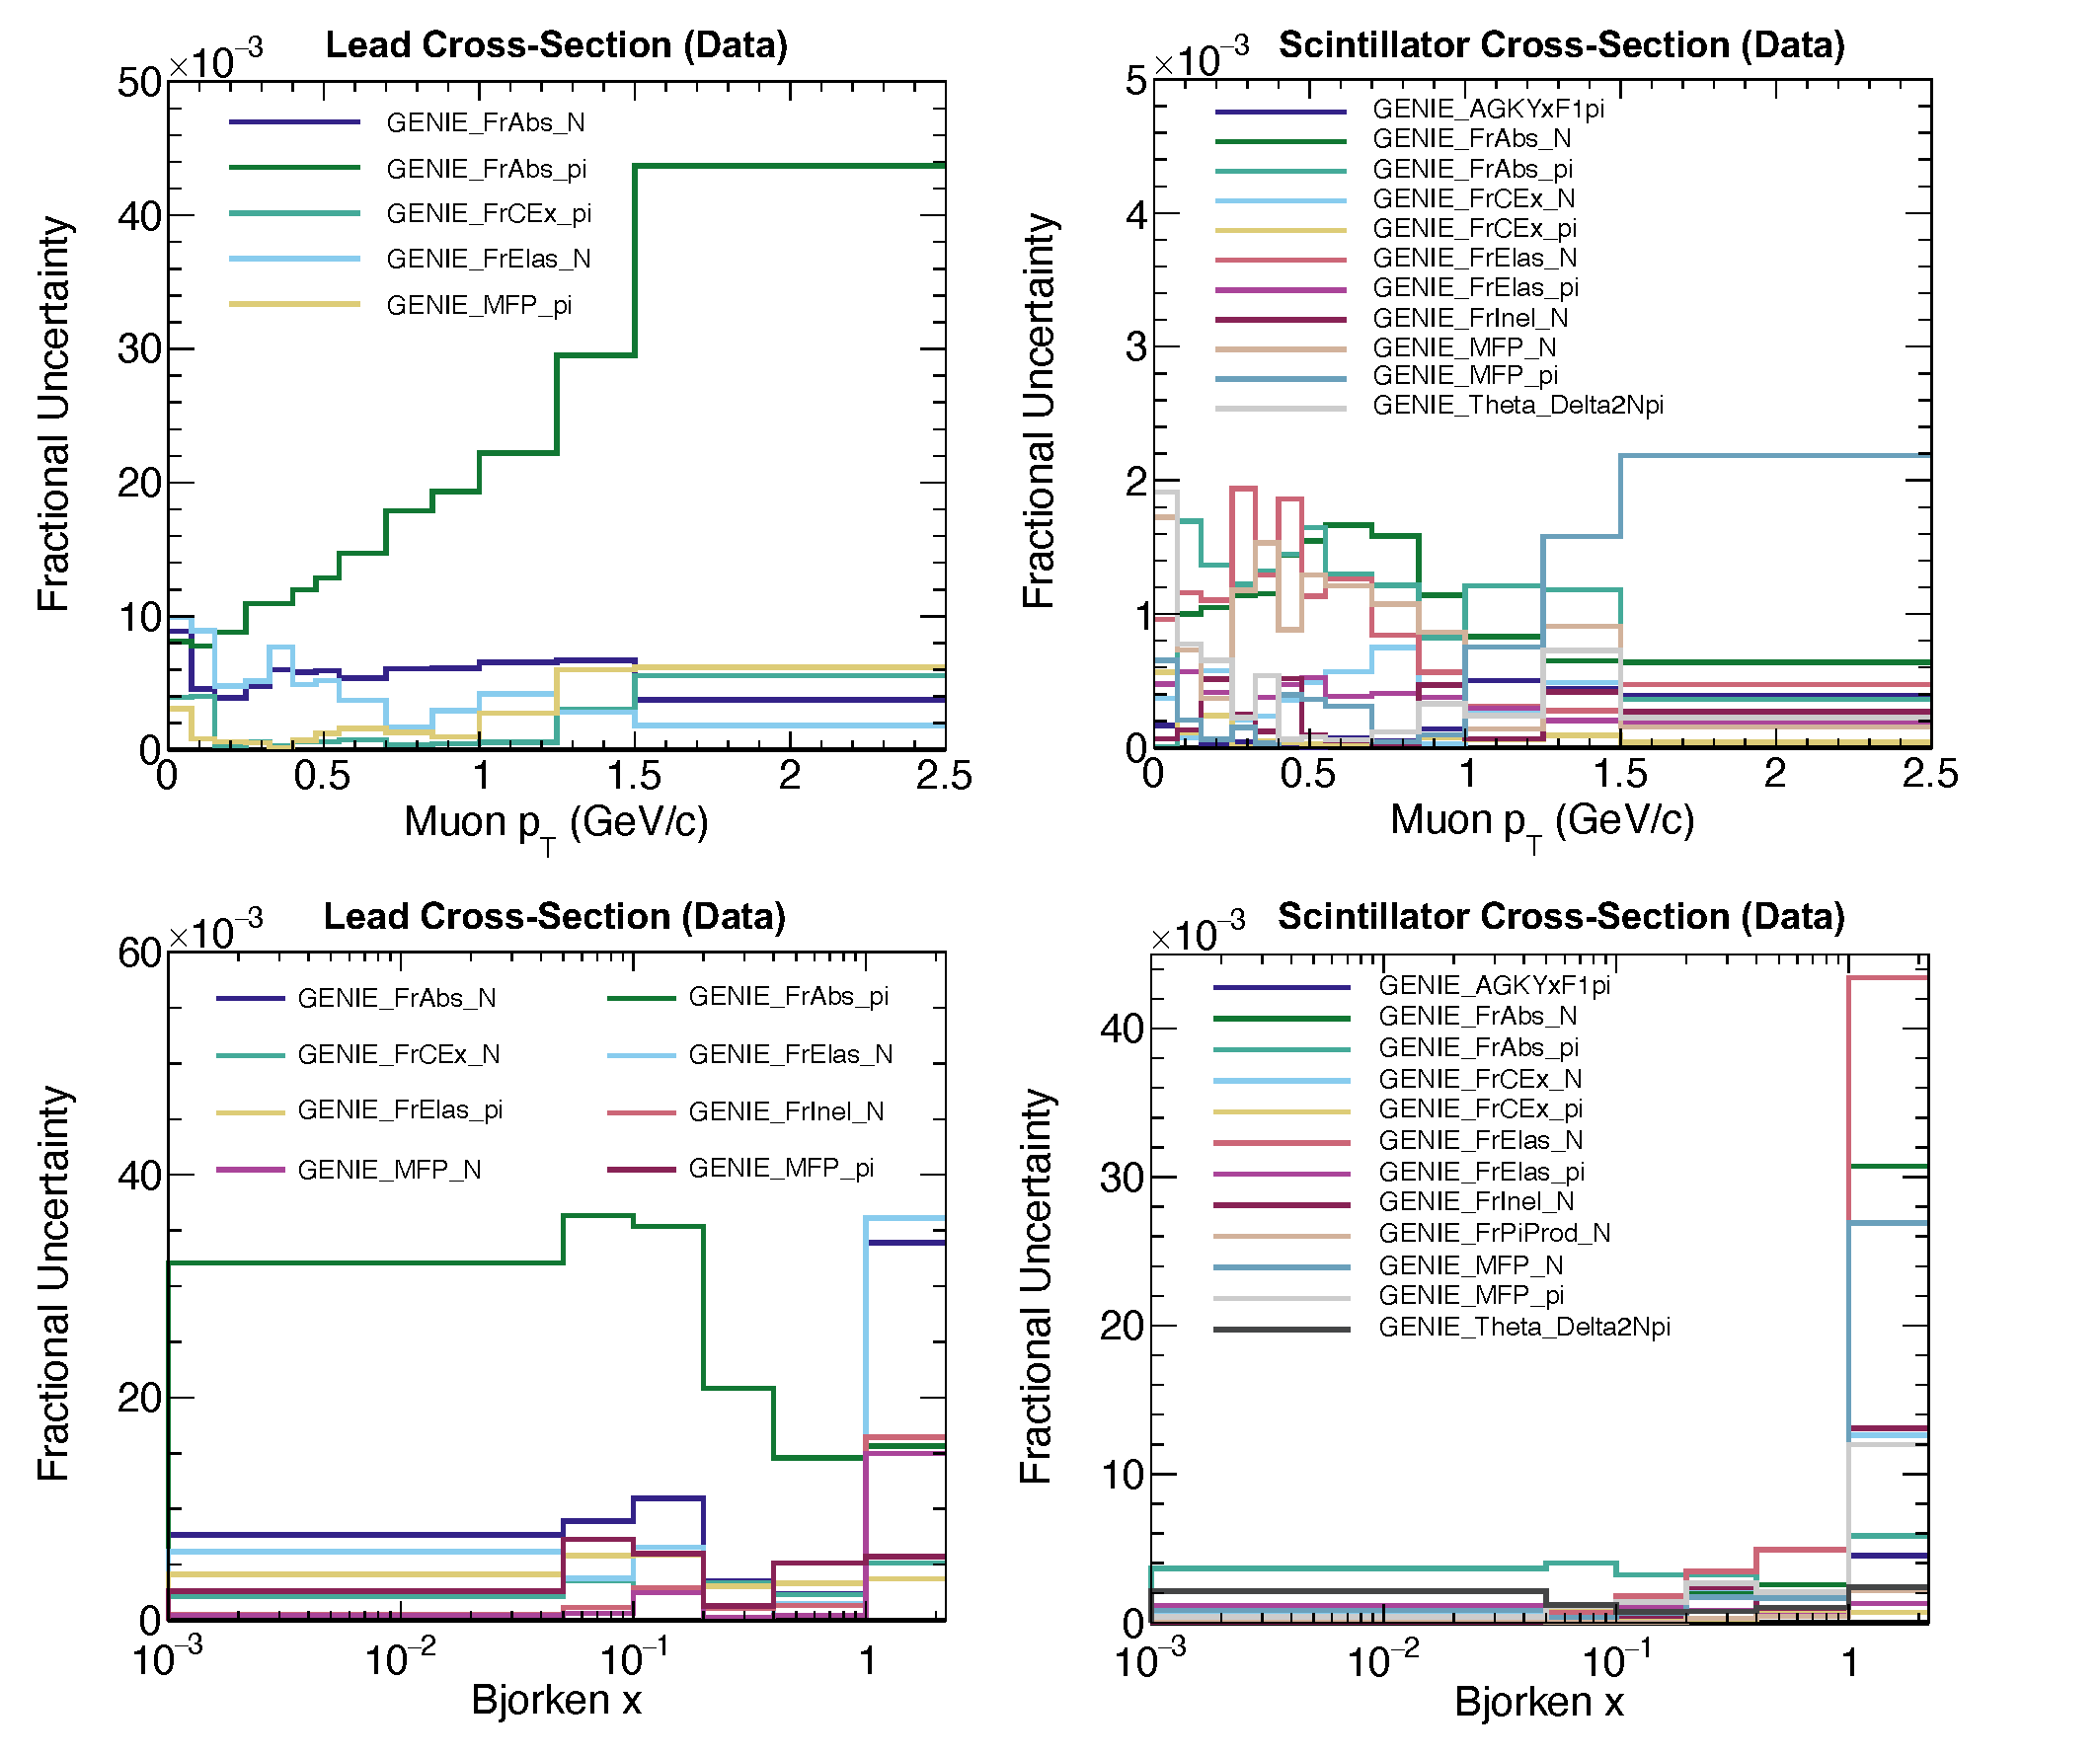
\includegraphics[width=1\textwidth]{08systematics/figures/fsi_t5leadTracker_pTx.pdf} }%
    \caption{Breakdown of various sources of uncertainty in the `FSI' error band of the differential cross-section in data, both in $p_{\text{T}}$ (top) and Bjorken $x$ (bottom) for lead (left panel) and scintillator (right panel). Note that only uncertainties that contribute more than 0.5\%  for lead and more than 0.05\% for scintillator are shown, illustrating the striking difference in the FSI uncertainty in heavier nuclei.}%
    \label{fig:fsi_t5leadTracker_pTx}
\end{figure}

The uncertainty on the final-state interactions (FSI) refers to the combination of uncertainties in GENIE parameters governing all interactions following the initial interaction. In this context, in addition to the uncertainties on the intranuclear cascade parameters, the `FSI' error band also includes uncertainties on hadronisation and delta resonance decay (which are technically not FSI). The uncertainties in these parameters implemented in GENIE were originally determined by the MINOS collaboration~\cite{dytman2008hadronic}.\enlargethispage{1\baselineskip} 

Figure~\ref{fig:fsi_t5leadTracker_pTx} displays uncertainties in the $p_{\text{T}}$ and Bjorken~$x$ differential cross-sections on lead and scintillator that contribute more than 0.5\% and more than 0.05\%, respectively, to the `FSI' uncertainty band. A close-up of the scintillator breakdown in Bjorken~$x$ in the $x<1$~region is included in Appendix~\ref{ch:appendix_sysUncertainties}. The comparison between the heavy lead and the light scintillator highlights the major difference in their respective `FSI' contributions. The larger `FSI' uncertainty in lead is associated with its complex nuclear environment, characterised by a significantly higher number of nucleons compared to the scintillator, which is primarily composed of carbon. In particular, the primary source of uncertainty contributing significantly to the `FSI' error band in lead is related to the uncertainty regarding the probability of a pion produced in the initial interaction being absorbed by the nuclear environment, resulting in it not exiting the nucleus. This is not unexpected as the pion production represents the dominant channel in this analysis. Table~\ref{table:FSIUnc} provides a list and description of all parameters associated with the uncertainties presented in Figure~\ref{fig:fsi_t5leadTracker_pTx}.

% What is xF https://www.phenix.bnl.gov/WWW/publish/seto/tutorials/notes%20on%20x_F%20and%20x_Bj%20for%20clarity.txt
% Note there was a bug in 2.12.6 in this (before this it was all isotropic) but not big impact at all on this analysis
% didn't fix it so it goes from anisotropic to more anisotropic
\begin{table}[b!]
    \centering
    \small
    \begin{tabularx}{1.0\textwidth}{c c L}
    \hline \\ [-1.5 ex]
    Error band & 1$\sigma$ & Description\\ [0.5ex] % inserts table %heading
    \hline
    \hline \\ [-2ex]
    AGKYxF1pi & $\pm20$\% & Modifies DIS hadronisation model for low multiplicity production of nucleons and pions \\
    FrAbs\_N & $\pm20$\% & Absorption probability for nucleons (for given total rescattering probability) \\
    FrAbs\_pi & $\pm30$\% & Absorption probability for pions (for given total rescattering probability) \\
    FrCEx\_N & $\pm50$\% & Charge exchange probability for nucleons (for given total rescattering probability)\\
    FrCEx\_pi & $\pm50$\% & Charge exchange probability for pions (for given total rescattering probability)\\
    FrElas\_N & $\pm30$\% & Elastic scattering probability for nucleons (for given total rescattering probability) \\
    FrElas\_N & $\pm10$\% & Elastic scattering probability for pions (for given total rescattering probability) \\
    FrInel\_N & $\pm40$\% & Inelastic scattering probability for nucleons (for given total rescattering probability) \\
    FrPiProd\_N & $\pm20$\% & Pion production probability for nucleons (for given total rescattering probability)\\
    MFP\_N &$\pm20$\%  & Modifies the mean free path for nucleons \\
    MFP\_pi & $\pm20$\% & Modifies the mean free path for pions \\
    Theta\_Delta2Npi & $\pm100$\% & Uncertainty on the anisotropy of the delta decay angular distribution \\
    \hline
    \end{tabularx}
    \caption{Description of various sources of uncertainty in the `FSI' error band from Figure~\ref{fig:fsi_t5leadTracker_pTx} with their corresponding 1$\sigma$ shifts.}
    \label{table:FSIUnc}
\end{table}

\section{Particle response}
%  no detector response uncertainty on muon variables (recoil reconstruction has no impact) in comparison to Bjorken x
% GEANT neutron modelling significant in both pT and Bjorken x - why?

\begin{figure}[b!]%
    \vspace{-7pt}
    \centering
   {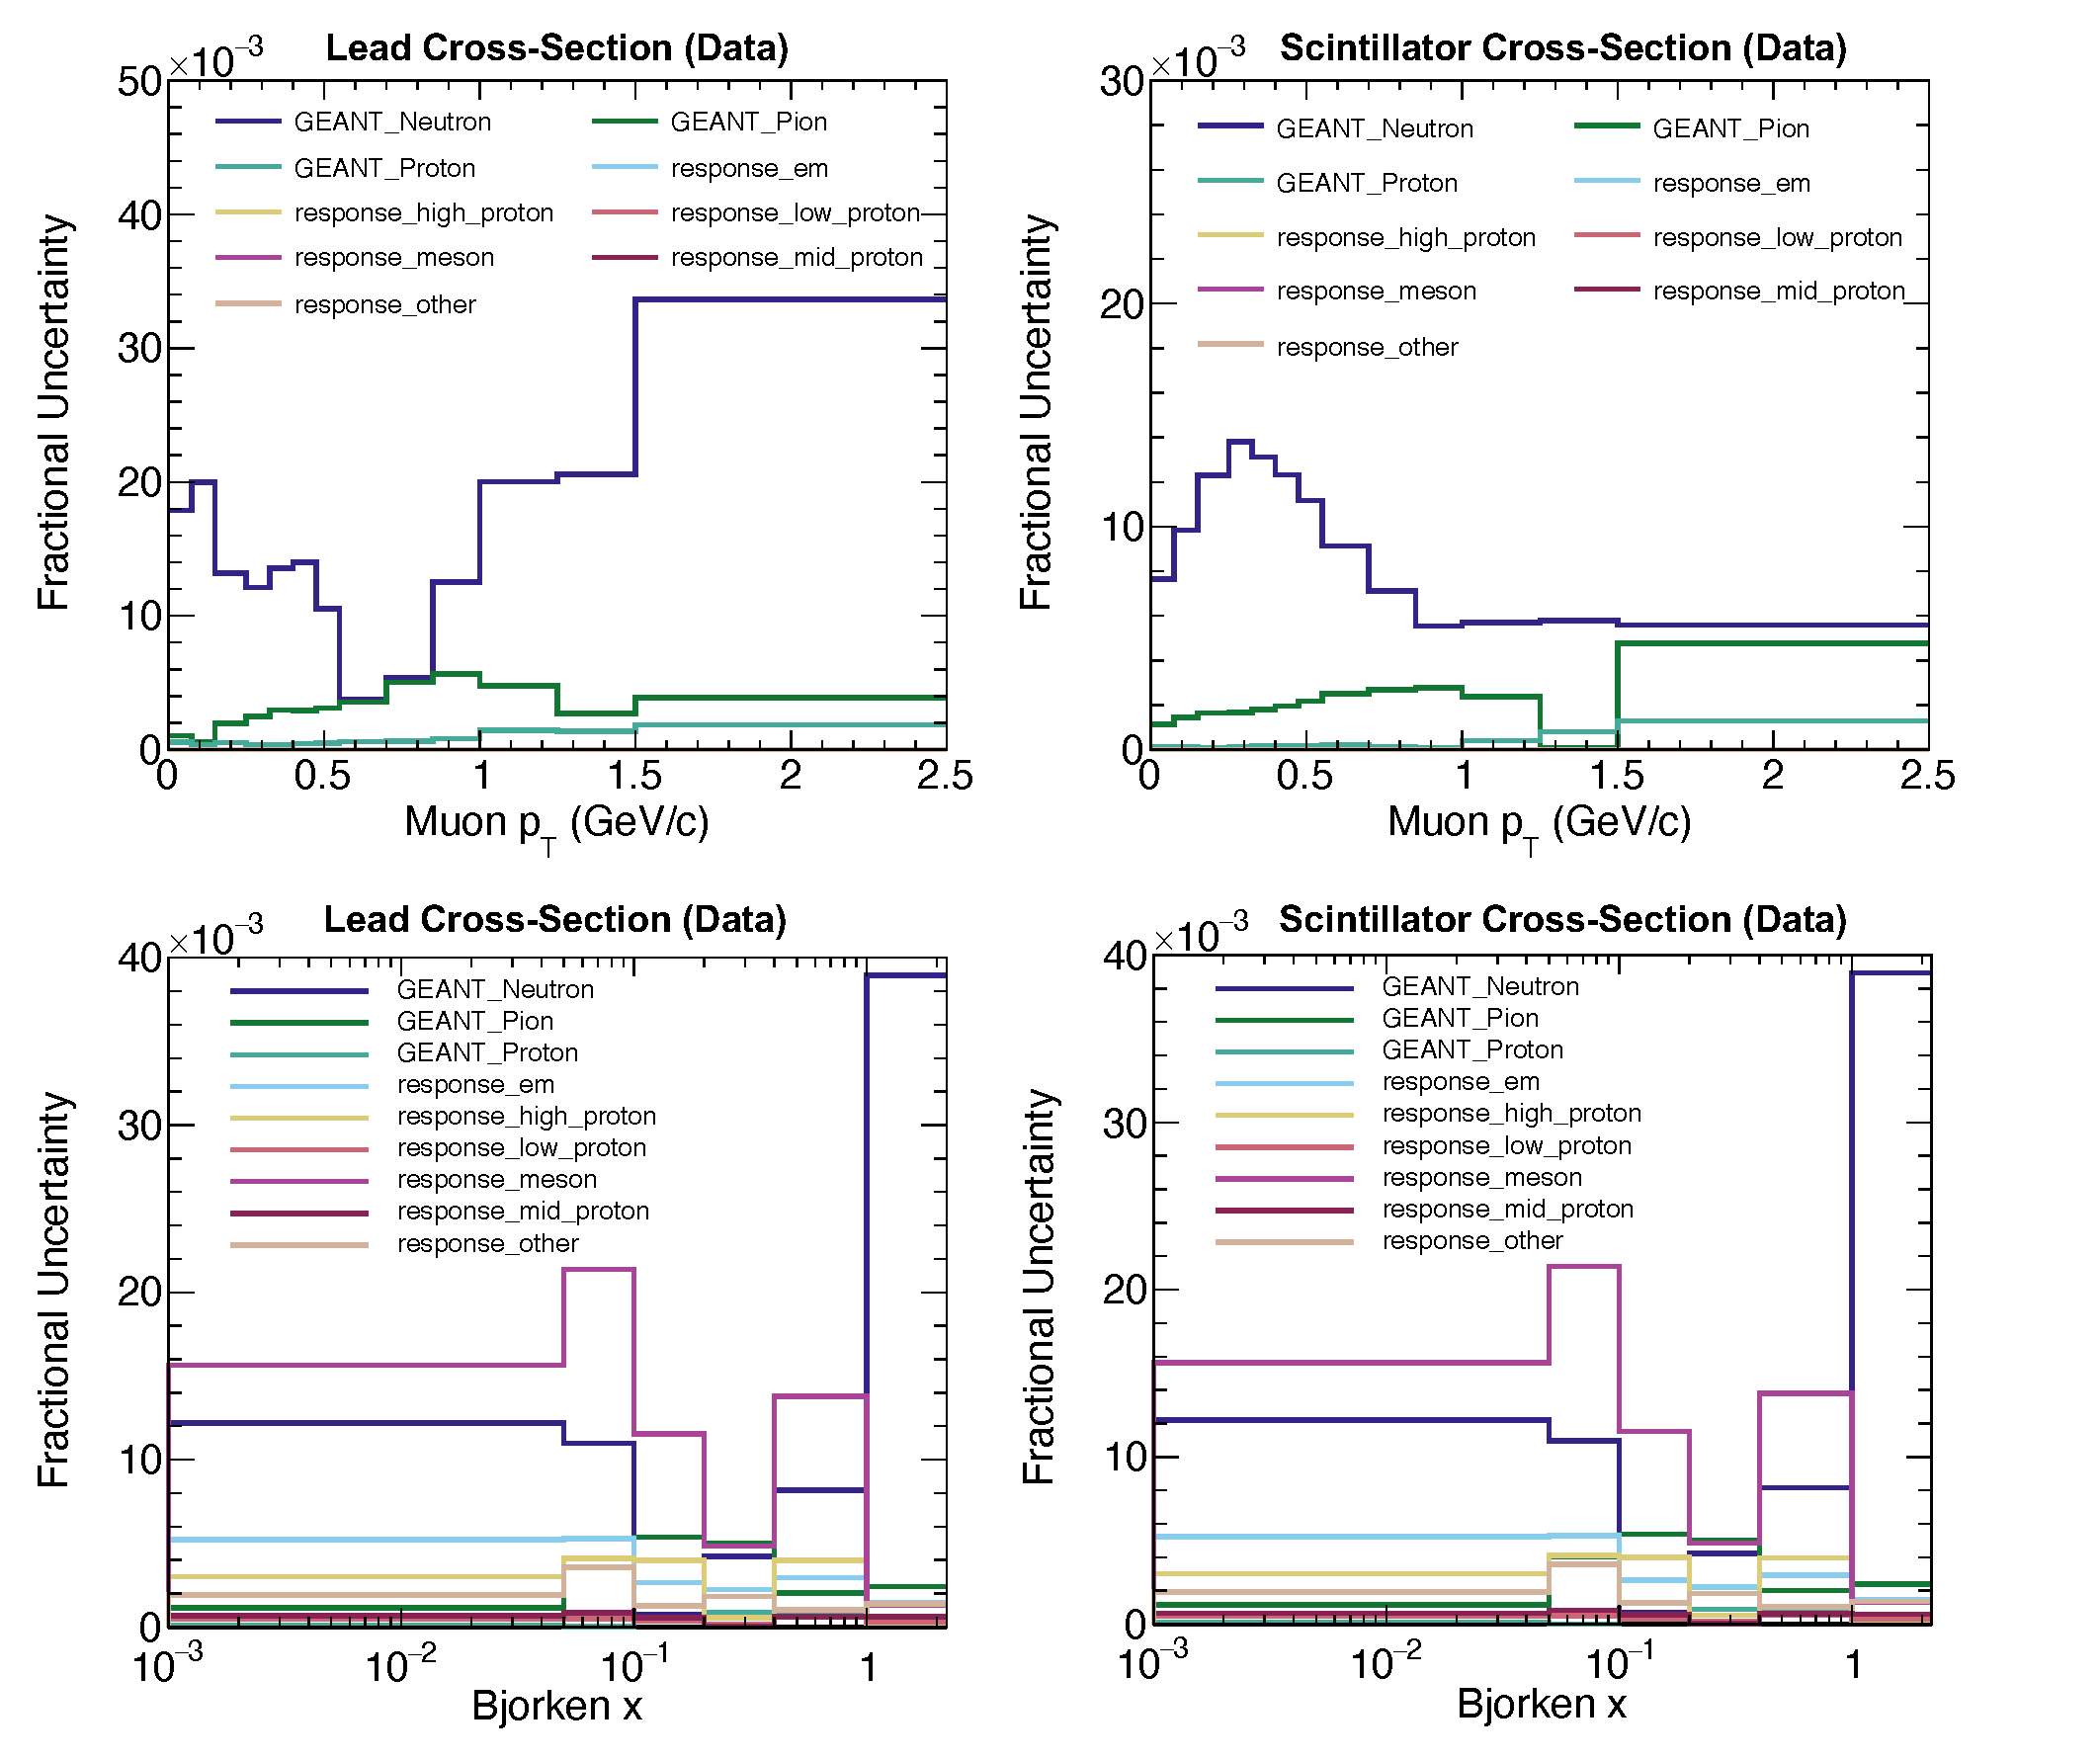
\includegraphics[width=1\textwidth]{08systematics/figures/response_t5leadTracker_pTx.pdf} }%
    \caption{Breakdown of various sources of uncertainty in the `Particle Response' error band of the differential cross-section in data, both in $p_{\text{T}}$ (top) and Bjorken $x$ (bottom) for lead (left panel) and scintillator (right panel). Note the additional contribution from uncertainties related to the calorimetric detector response relevant to recoil reconstruction in Bjorken $x$.}%
    \label{fig:response_t5leadTracker_pTx}
\end{figure}

The `Particle Response' error band in Figures~\ref{fig:mcSimulationFracUnc_t5lead_pTx} and~\ref{fig:crossSectionFracUnc_lead_pTx} includes uncertainties concerning both the interaction cross-sections used by GEANT4~\cite{Geant4_AGOSTINELLI2003250, Geant4_1610988} for simulating final-state particles as they traverse the MINERvA detector (discussed in Chapter~\ref{ch:dataAsimulation}) and the calorimetric detector response relevant to recoil reconstruction (described in Chapter~\ref{ch:Reconstruction}). Figure~\ref{fig:response_t5leadTracker_pTx} breaks down the sources of uncertainties contributing to this error band in the $p_{\text{T}}$ and Bjorken~$x$ differential cross-sections on lead and scintillator.\enlargethispage{1.\baselineskip} 

To evaluate the uncertainty associated with the GEANT4 simulation, MINERvA varies the hadronic inelastic cross-section of the final-state protons and pions based on the MINERvA test beam data~\cite{ALIAGA201528}~according to the procedure described in Subsection~\ref{sec:particleProp}. The uncertainty on the neutron inelastic cross-section reflects the reweight to the Abfalterer \textit{et al.}~data~\cite{Abfalterer_PhysRevC.63.044608} also outlined in Subsection~\ref{sec:particleProp}. The GEANT4 neutron uncertainty also accounts for the uncertainty on neutron energy deposits, as the neutron energy deposition is dependent on the neutron inelastic cross-section.
% https://minerva-docdb.fnal.gov/cgi-bin/sso/ShowDocument?docid=7532
% 10\% C carbon, 15\% iron, 20\% lead for protons and pions

% GEANT systematics: % Systematics!! For example, for total inelastic cross-section for protons and pions, the variation is 10\% in carbon and hydrocarbon, 15\% in iron and 20\% in lead. Similarly, the neutron interaction cross-section is reweighted 
%https://minerva-docdb.fnal.gov/cgi-bin/sso/RetrieveFile?docid=7532&filename=dytman-hadr-uncert-27apr12.pdf&version=2

The uncertainties on how the MINERvA detector responds to various calorimetric recoil energy deposits from protons~\cite{protonTestbeam} and pions~\cite{pionTestbeam} are also constrained by the test beam studies~\cite{ALIAGA201528}. The electromagnetic response uncertainty is derived from differences between data and simulation when observing Michel electrons (electrons from muon decay)~\cite{Aliaga_2014}. Other unconstrained contributions are assigned conservative uncertainties. All these uncertainties for various particle energy deposits are summarised in Table~\ref{table:responseUnc}.

The comparison between lead and scintillator in Figure~\ref{fig:response_t5leadTracker_pTx} highlights that uncertainties in the modelling of inelastic cross-sections are more pronounced for heavier targets. Overall, the uncertainty on neutron modelling is the largest, contributing significantly to both $p_{\text{T}}$ and Bjorken~$x$ distribution. In $p_{\text{T}}$ in particular, the effect is attributed to correlations between the outgoing particle kinematics, with $p_{\text{T}}$ serving as a proxy for the momentum transfer. Furthermore, as expected, uncertainties in the calorimetric response of the detector have a significant impact on the Bjorken~$x$ distribution, in contrast to the~$p_{\text{T}}$ distribution, which, by definition, does not depend on recoil reconstruction. Note that in Bjorken $x$, the dominant source of uncertainty corresponds to the detector's response to pions (mesons), consistent with pion production constituting the primary channel in this analysis. \enlargethispage{1.\baselineskip} 

\begin{table}[b!]
    \centering
    \small
    \begin{tabularx}{0.94\textwidth}{c c L}
    \hline \\ [-1.5 ex]
    Error band & 1$\sigma$ & Description\\ [0.5ex] % inserts table %heading
    \hline
    \hline \\ [-2.0ex]
    response\_low\_proton & $\pm4.0$\% & Proton kinetic energy $< 50$ MeV \\
    response\_mid\_proton & $\pm3.5$\%  & Proton kinetic energy between $50$ MeV and $100$ MeV\\
    response\_high\_proton & $\pm3.0$\%  & Proton kinetic energy $> 100$ MeV  \\
    response\_meson & $\pm5.0$\%  & Pion kinetic energy between $400$ MeV and $1.9$ GeV \\
    response\_em & $ \pm3.0$\%  & Electromagnetic shower  \\
    response\_other & $\pm20.0$\%  &  Other \\
    \hline
    \end{tabularx}
    \caption{Description of various sources of uncertainty related to the calorimetric detector response relevant to recoil reconstruction in the `Particle Response' error band from Figure~\ref{fig:response_t5leadTracker_pTx} with their corresponding 1$\sigma$ shifts.}
    \label{table:responseUnc}
\end{table}

\section{Other}
% - ML vertex and uncertainty on target mass

Other uncertainties considered in this analysis are related to the material mass and the machine-learning-based vertex reconstruction. Specifically, the estimated uncertainties on the fiducial masses due to density and thickness variations are represented by $\pm0.5$\% shifts for the carbon and lead mass, $\pm1.0$\% for the iron mass, and $\pm1.4$\% for the scintillator mass~\cite{Aliaga_2014}. The uncertainty associated with the ability to correctly resolve the vertex position using machine learning is set conservatively by $\pm1.0$\% shifts relative to the central value based on my studies of the differences between the data and the simulation in the plane prediction distributions for antineutrino interaction vertices~\cite{Klustova_MLsys}. The `Other' error band in Figures~\ref{fig:mcSimulationFracUnc_t5lead_pTx} and~\ref{fig:crossSectionFracUnc_lead_pTx} represents the combination of these two uncertainties above and contributes slightly over 1\% to the total uncertainty in the differential cross-section. 

\section{Additional sources of uncertainties}
%- uncertainty on the sideband fit scale factor - added in quadrature to the statistical + systematic uncertainty
%- neutron/missing energy uncertainty 

Two additional systematic uncertainties arising from two aspects of the analysis procedure described in Chapter~\ref{ch:analysis1D}~are under consideration for implementation. Specifically, an uncertainty is proposed to account for the disagreement between the data and simulation after the data-driven plastic sideband fit procedure, outlined in Section~\ref{sec:bkgSubtraction}. This proposed uncertainty is aimed at addressing discrepancies that are not, in some bins, fully covered by the current list of systematic uncertainties. Alternatively, the shape differences could be mitigated by introducing a bin-by-bin scale factor, potentially eliminating the need for this additional systematic uncertainty, which is further discussed in Chapter~\ref{ch:results}.

Additionally, another uncertainty could account for potential model bias in the Bjor\-ken~$x$ cross-section introduced by the neutron modelling corrections at the unfolding level suggested by the exploratory study in Section~\ref{sec:migration_unfolding}. This proposed uncertainty would address the differences observed in the $x > 1$ region when unfolding data using simulations with modified true invisible energy distributions, as shown in Figure~\ref{fig:maresCheck_invisECheck} in the relevant section.\enlargethispage{1.5\baselineskip} However, in order to do so, it is essential to examine and understand the magnitude of the variations in invisible energy first. 
\clearpage
\thispagestyle{empty}
\hfill
\clearpage
\chapter{Results and discussion}

\label{ch:results} 

% Aaron:  https://arxiv.org/pdf/2209.07852.pdf
% Jeffrey: https://minerva-docdb.fnal.gov/cgi-bin/sso/RetrieveFile?docid=31903&filename=MINERvA_Nucl_Target_PRD_based_on_JK_analysis%20%282%29.pdf&version=2

This chapter presents the results and the related discussion of the nuclear dependence measurement in antineutrino scattering using MINERvA, the analysis that I conducted and detailed in this work. Specifically, the cross-section results include differential cross-sections in antimuon $p_{\text{T}}$ and Bjorken $x$ for carbon, hydrocarbon (scintillator), iron, and lead, along with their associated uncertainty breakdowns.

Additionally, the chapter features ratios of carbon-, iron-, and lead-to-hydrocarbon in both variables of interest, each with corresponding uncertainty breakdowns. These comparisons effectively highlight (mostly) flux-independent differences between the different nuclei. While the chapter includes all cross-section and cross-section ratio results, the discussion focuses on and summarises observed general trends. The discussion also considers potential future improvements to the analysis.

Furthermore, the cross-section and cross-section ratio results are reviewed in the context of other (anti)neutrino event generators. In particular, the results are compared with a newer version of GENIE and with NEUT, which employ different interaction models than the underlying simulation.

[2D extension note]

\section{Antimuon~$p_{\text{T}}$ results}

% Say how many events, compare to the LE sample [ REF]

Figure~\ref{fig:xsec_pT} shows the extracted differential cross-sections in antimuon transverse momentum $p_{\text{T}}$ for inclusive antineutrino scattering on carbon, hydrocarbon (scintillator), iron, and lead, while Figure~\ref{fig:ratio_pT} illustrates the corresponding nuclear target-to-scintillator ratios. As explained in Chapter~\ref{ch:measurement}, $p_{\text{T}}$ serves as a convenient recoil energy independent proxy to the square of the four-momentum transferred, $Q^2$, in the course of the scattering process. Therefore, the peaks of the individual interaction type contribution in the simulation prediction breakdown in Figure~\ref{fig:xsec_pT} can be visibly seen to follow the low-transfer to high-transfer ordering from low-$p_{\text{T}}$ to high-$p_{\text{T}}$ region, indicating that quasi-elastic scattering and 2p2h mainly contribute at low $p_{\text{T}}$, whereas the deep inelastic scattering tends to dominate at high $p_{\text{T}}$. However, overall, the cross-section is predicted to be dominated by the resonant pion production (even at lowest $p_{\text{T}}$) followed by the deep inelastic scattering as this analysis utilises MINERvA's medium energy dataset with antineutrino flux peak near $6$~GeV.

\begin{figure}[t!] 
    \vspace{20pt}
    \centering
    {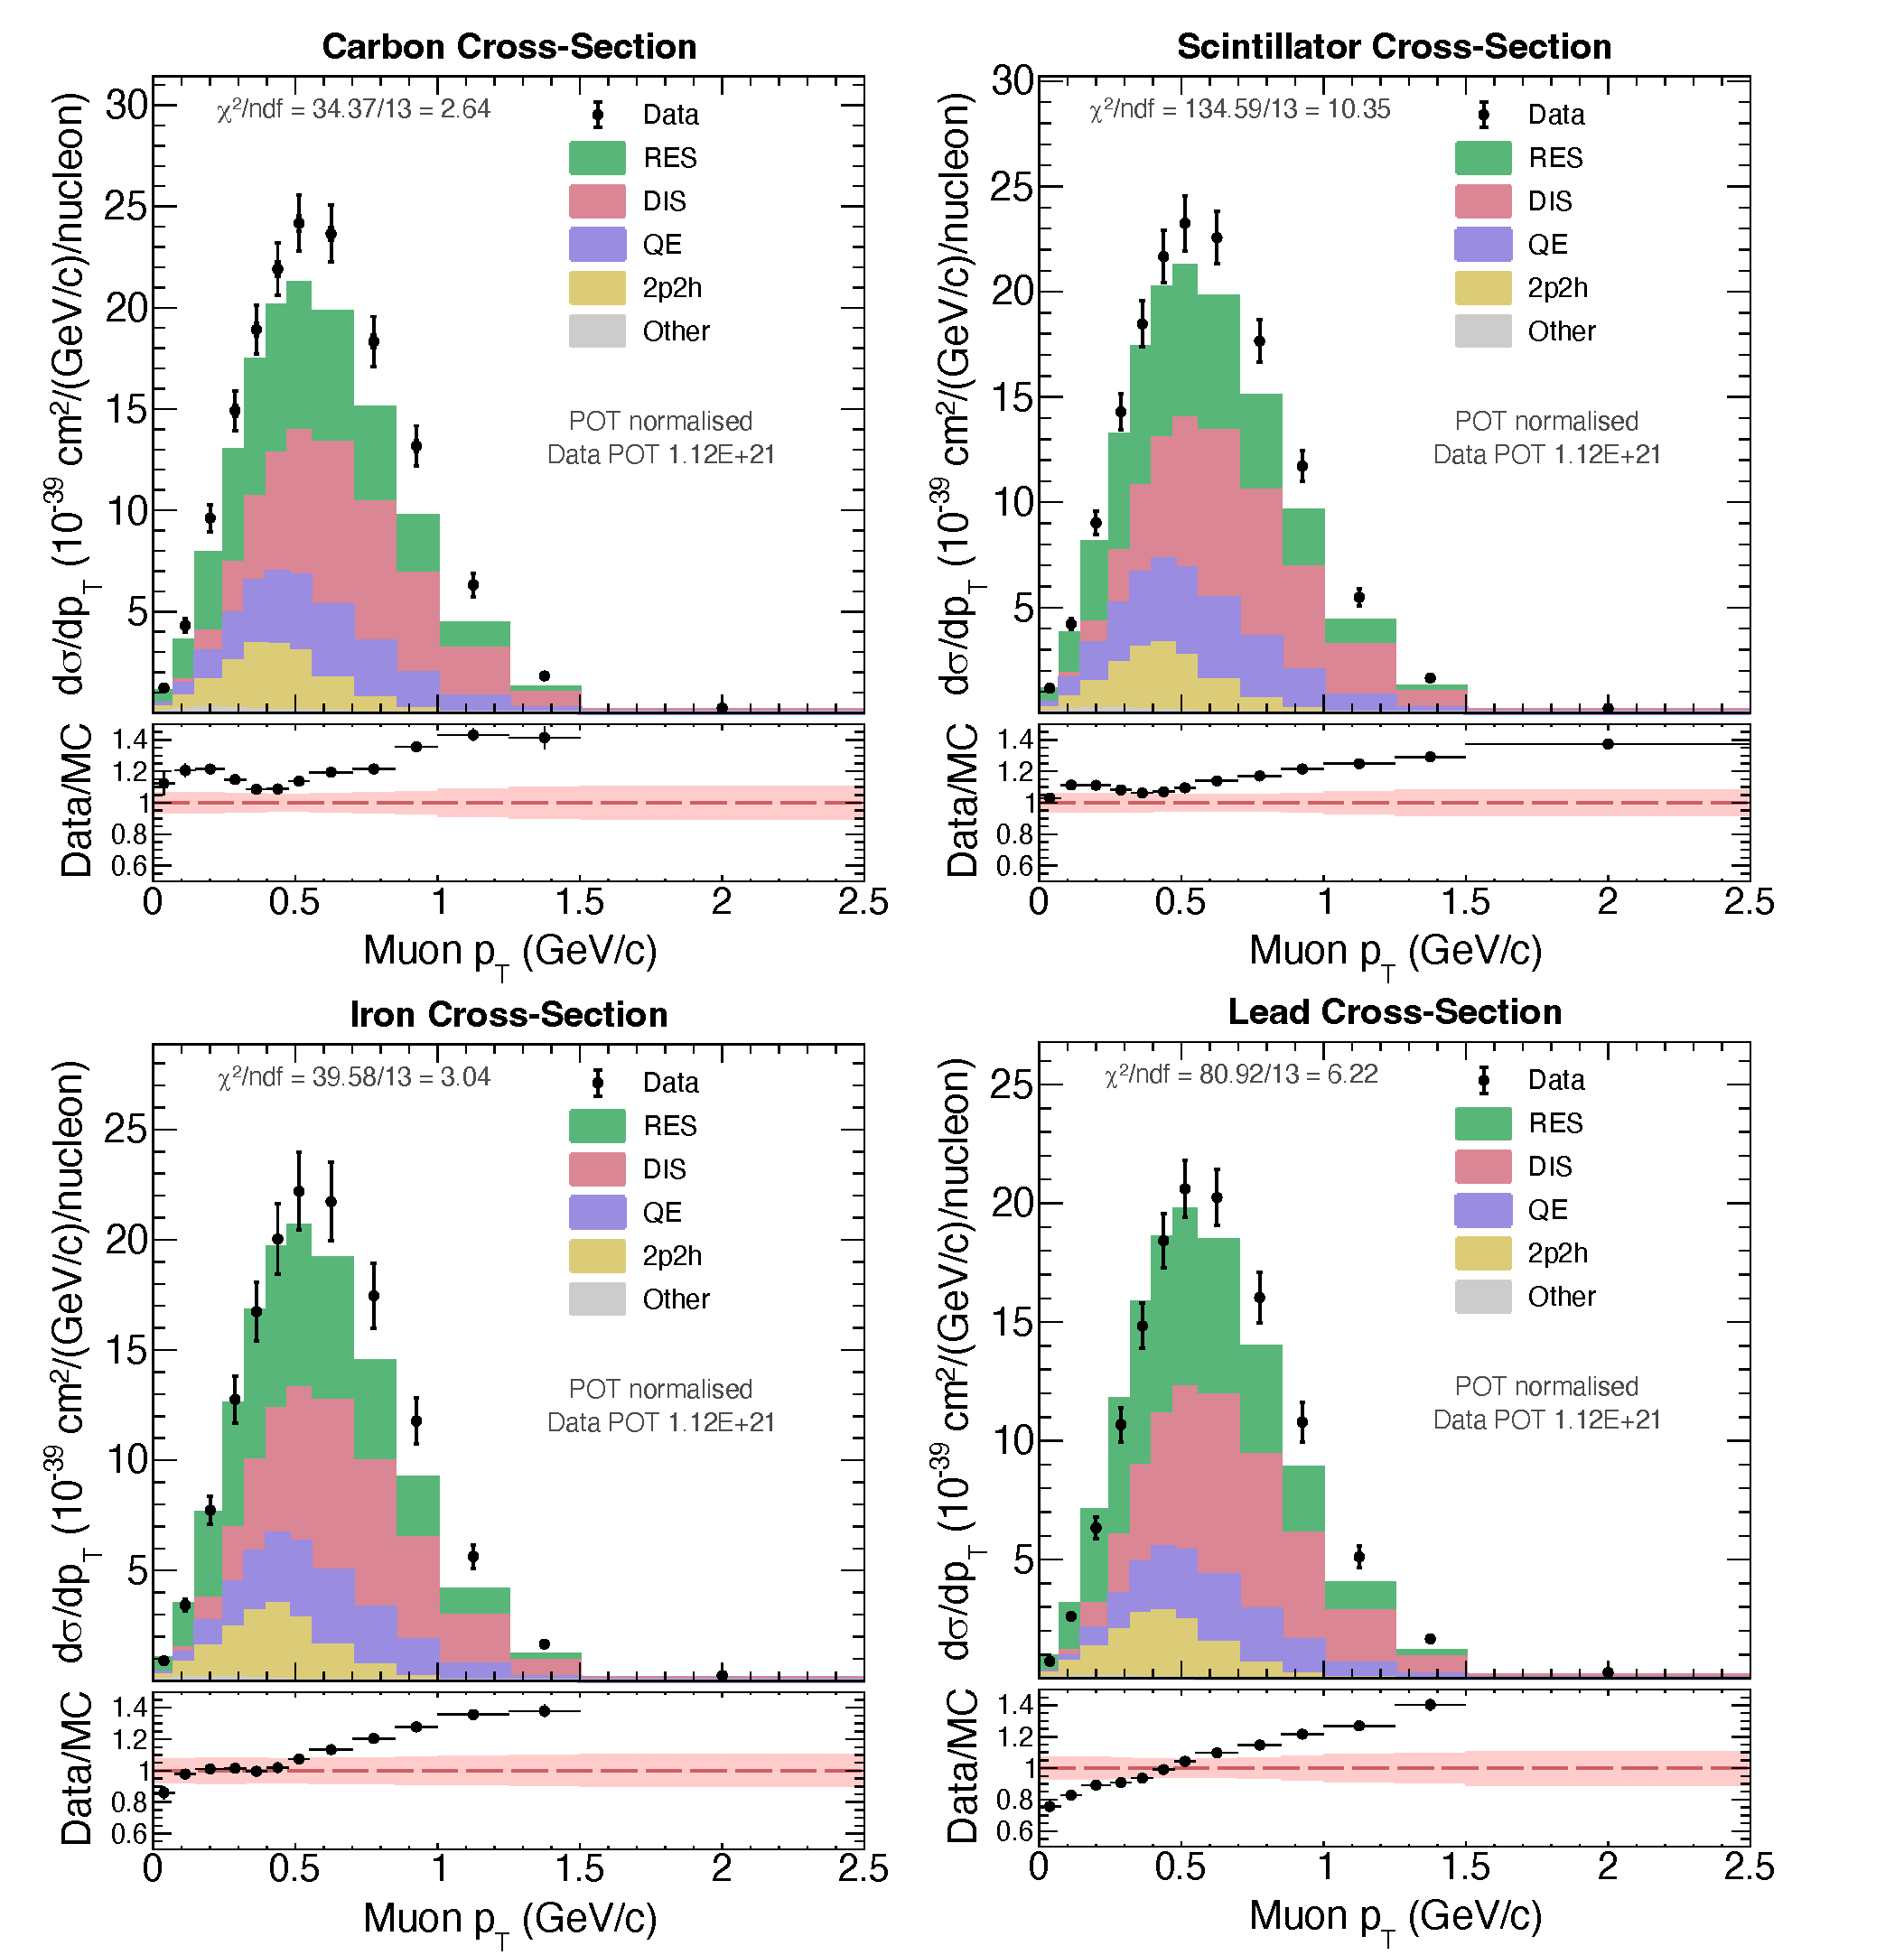
\includegraphics[width=1.\textwidth]{09results/figures/xsec_pT.pdf}}%
    \caption{Carbon, scintillator, iron, and lead (from left to right, top to bottom) cross-section as a function of $p_{\text{T}}$ with the simulation broken down into the various interaction channels stacked in the descending order of their contribution. In the top panel of each plot, the data points carry both statistical (inner error bar) and systematic (outer error bar, which is the sum of statistical and systematic errors) uncertainties. The bottom panel of each plot displays the data-to-simulation ratio, with the pink band around 1 representing systematic uncertainty on the data, while the black points reflect the statistical uncertainty on the data-to-simulation ratio.}
    \label{fig:xsec_pT}
\end{figure}


Importantly, the data-to-simulation ratios in Figure~\ref{fig:xsec_pT} reflect the trend observed throughout the analysis process. The region from the falling edge of the $p_{\text{T}}$ distribution to large $p_{\text{T}}$ is systematically underpredicted by the simulation for all nuclei. The data excess grows as $p_{\text{T}}$ increases. Interestingly, a similar excess was reported in MINERvA's measurement of antineutrino quasi-elastic-like scattering only~\cite{PhysRevD.108.032018}. This indicates that either quasi-elastic scattering or resonant pion production, or a combination thereof, is being mismodelled, i.e. underpredicted, by the underlying simulation. 


Furthermore, the low $p_{\text{T}}$ region presents an interesting insight into the nuclear dependence of the inclusive antineutrino scattering, which is mostly ascribed to the resonant pion production in the simulation. The simulation prediction ranges from underprediction of the data for relatively light nuclei, i.e. low-$A$ carbon and hydrocarbon, to significant overprediction of the data for high-$A$ lead. In other words, the discrepancy changes and grows as a function of the mass number $A$. Notably, this has been seen in MINERvA's medium-energy neutrino charged-current single $\pi^+$ production on various nuclear targets~\cite{Bercellie2023_PhysRevLett.131.011801}. The low $Q^2$ suppression was also featured in several other datasets including MINOS neutrino measurement on iron~\cite{PhysRevD.91.012005}, and MINERvA low-energy measurements of neutrino pion production on the scintillator~\cite{PhysRevD.92.092008, PhysRevD.94.052005, PhysRevD.96.072003, PhysRevD.100.072005} and one low-energy antineutrino pion induced production also on the scintillator~\cite{PhysRevD.94.052005}. This analysis' result is the first such observation in an antineutrino dataset in medium energy across various nuclei. 

% RATIOS
\begin{figure}[t!] 
    \centering
    {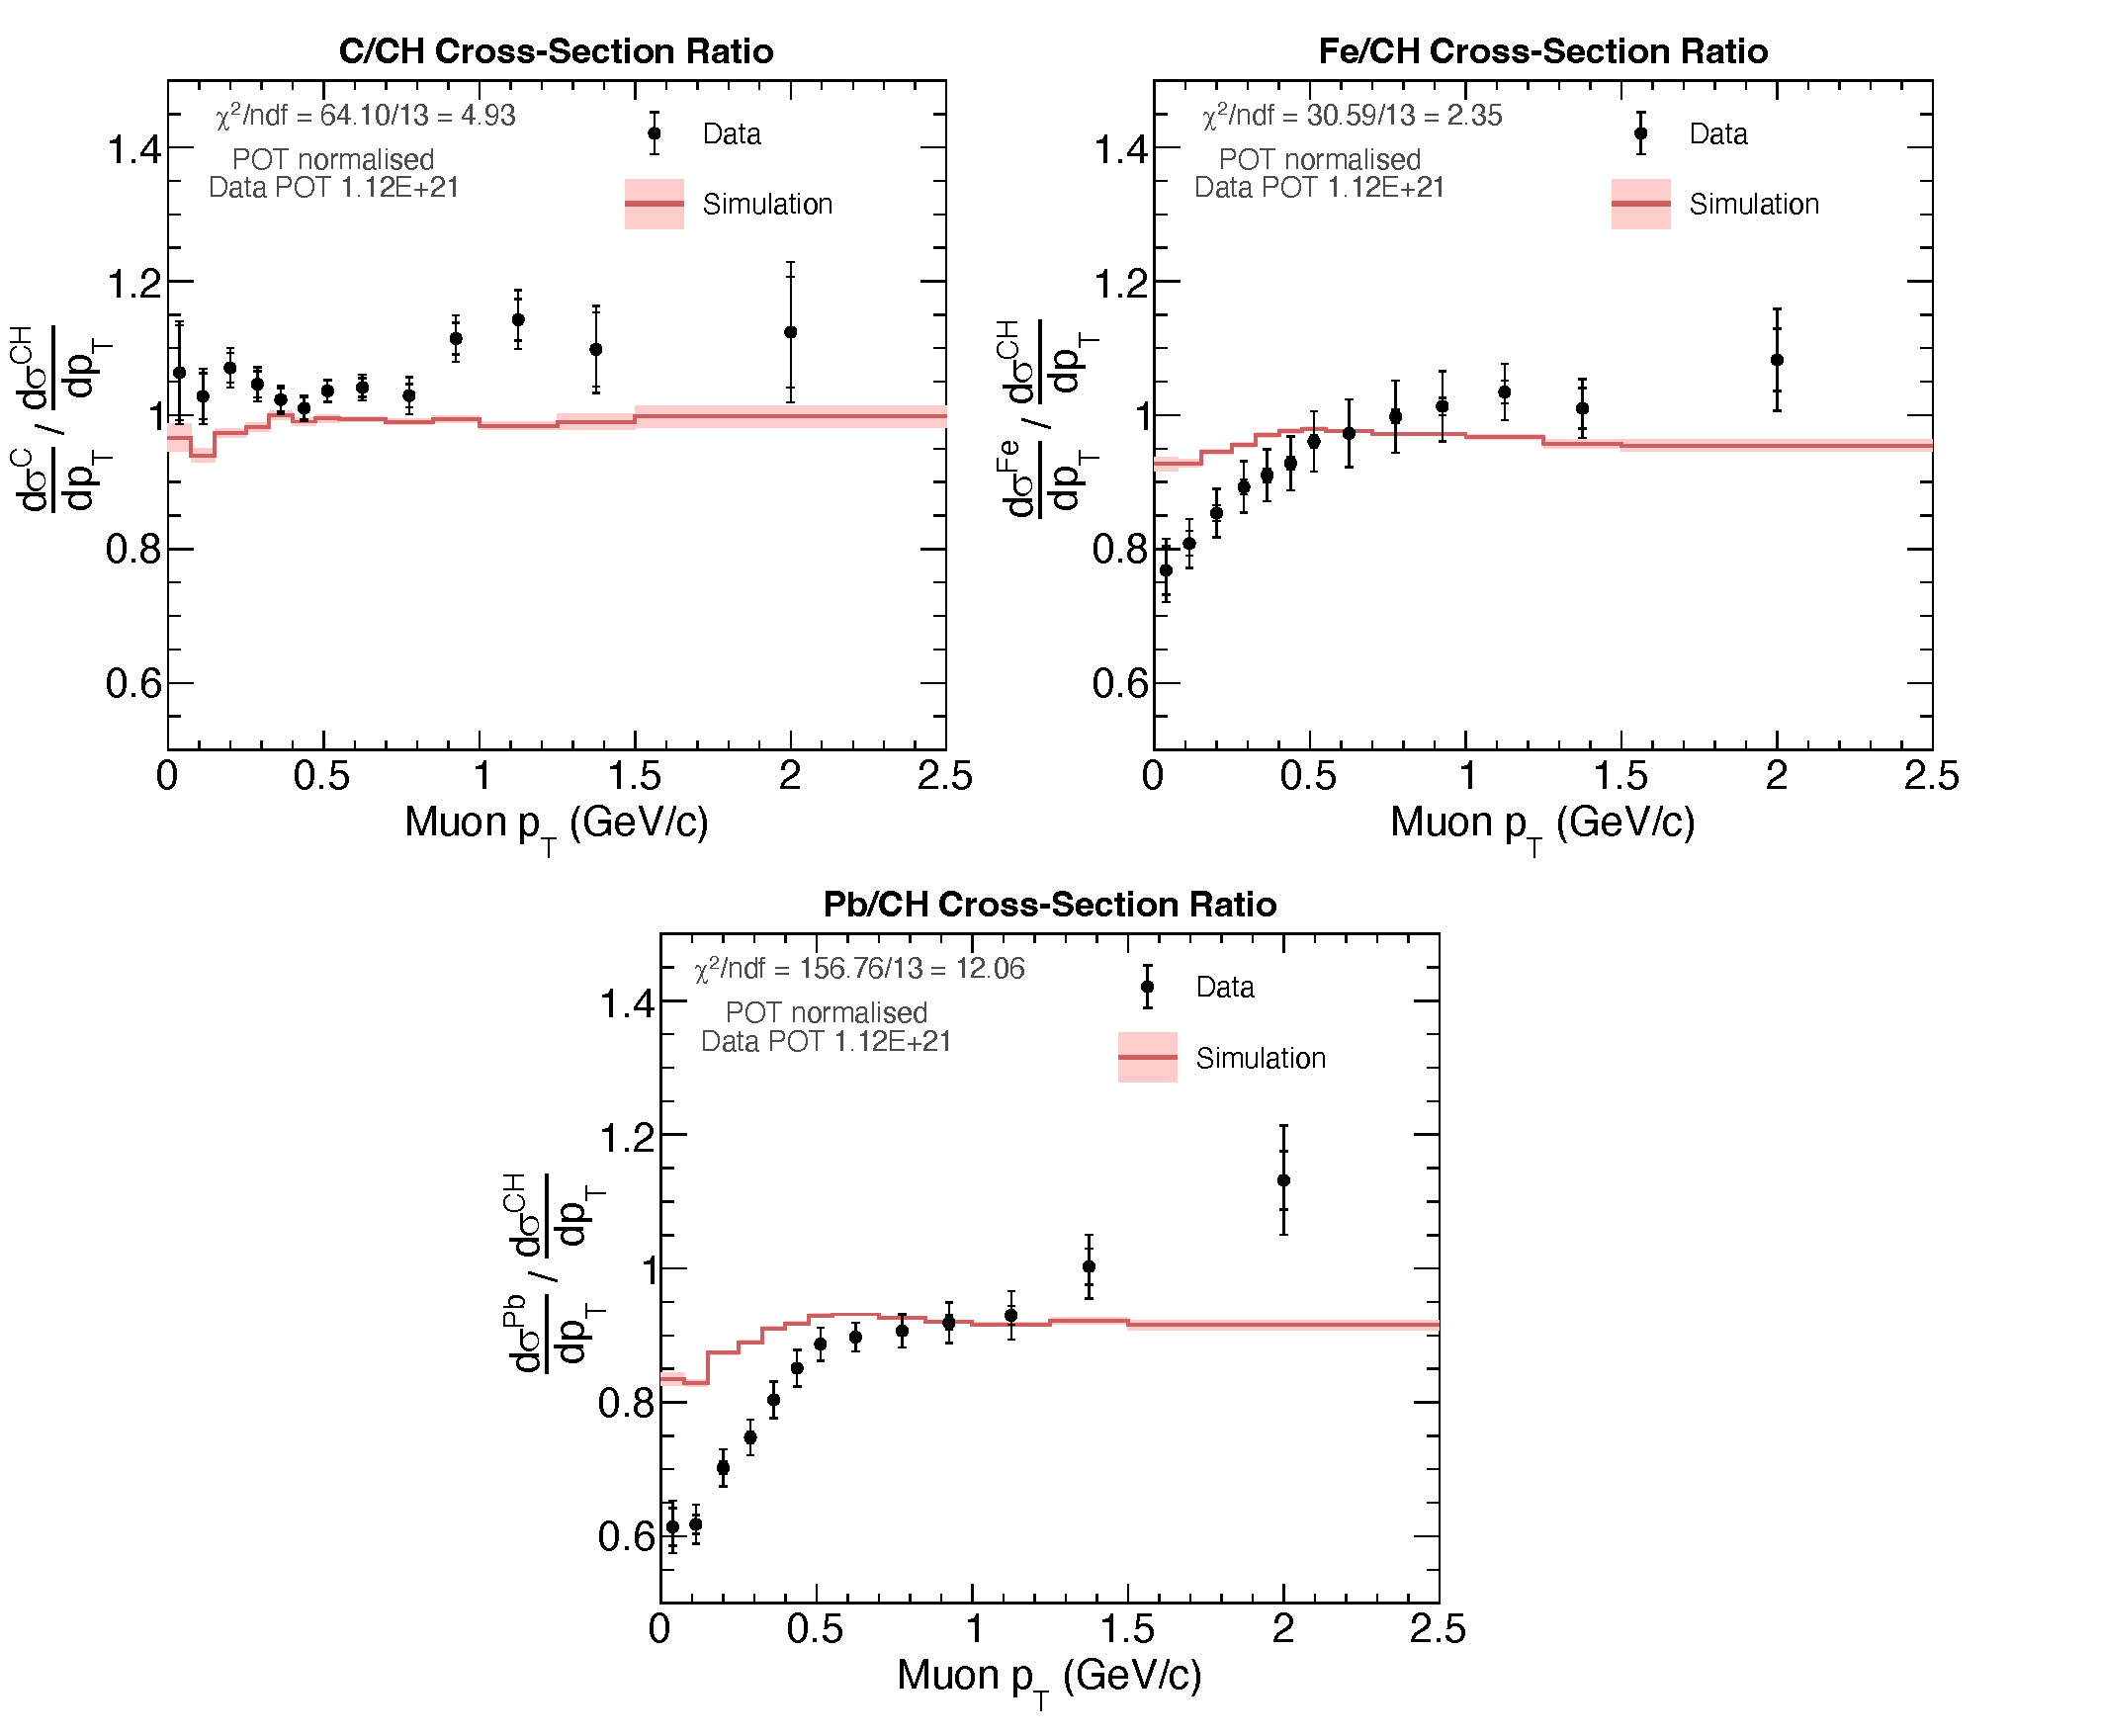
\includegraphics[width=1.\textwidth]{09results/figures/ratios_pT.pdf}}%
    \caption{Carbon-to-scintillator (top left), iron-to-scintillator (top right), and lead-to-scintillator (bottom) cross-section ratios in antimuon $p_{\text{T}}$. The data points carry both statistical (inner error bar) and systematic (outer error bar, which is the sum of statistical and systematic errors) uncertainties. The error band around the simulation predictions represents its statistical error. Note the significant $A$-dependence across the measured ratios, particularly in the low-$p_{\text{T}}$ region.}
    \label{fig:ratio_pT}
\end{figure}

As described in Chapter~\ref{ch:dataAsimulation}, this analysis tried to partially remedy the suppression by reweighting its single pion production, both resonant and non-resonant, with $\pi^-$ in final states, to match the low $Q^2$ (low $p_{\text{T}}$) suppression observed in the medium-energy single $\pi^+$ production on scintillator~\cite{Bercellie2023_PhysRevLett.131.011801}. While
the interpolation from neutrino to antineutrino mode was not necessarily expected to work, the suppression improved the simulation agreement with the data which is demonstrated in Appendix~\ref{ch:appendix_tuneComparisons}. The results show that this suppression seems to partially capture antineutrino interactions on iron, but it is not strong enough for lead. 

These observed trends are further amplified by looking at the carbon-, iron-, and lead-to-scintillator ratios in Figure~\ref{fig:ratio_pT}. While the carbon-to-scintillator ratio in antimuon $p_{\text{T}}$ is relatively flat as expected, the iron-to-scintillator and lead-to-scintillator ratios demonstrate dramatic $A$-scaling changes as a function of $p_{\text{T}}$, specifically at low and high $p_{\text{T}}$ as mentioned above. Overall these results suggest that both the total cross-section scaling versus $A$ and the low $Q^2$ suppression are larger than modelled and that the effect increases with increasing $p_{\text{T}}$ (square of the four-momentum transfer). Crucially, while the low $Q^2$ suppression is based on the pion production measurements, the inclusive antineutrino analysis spans other interaction channels that may contribute to the suppression observed in this region.

\begin{figure}[t!] 
    \centering
    {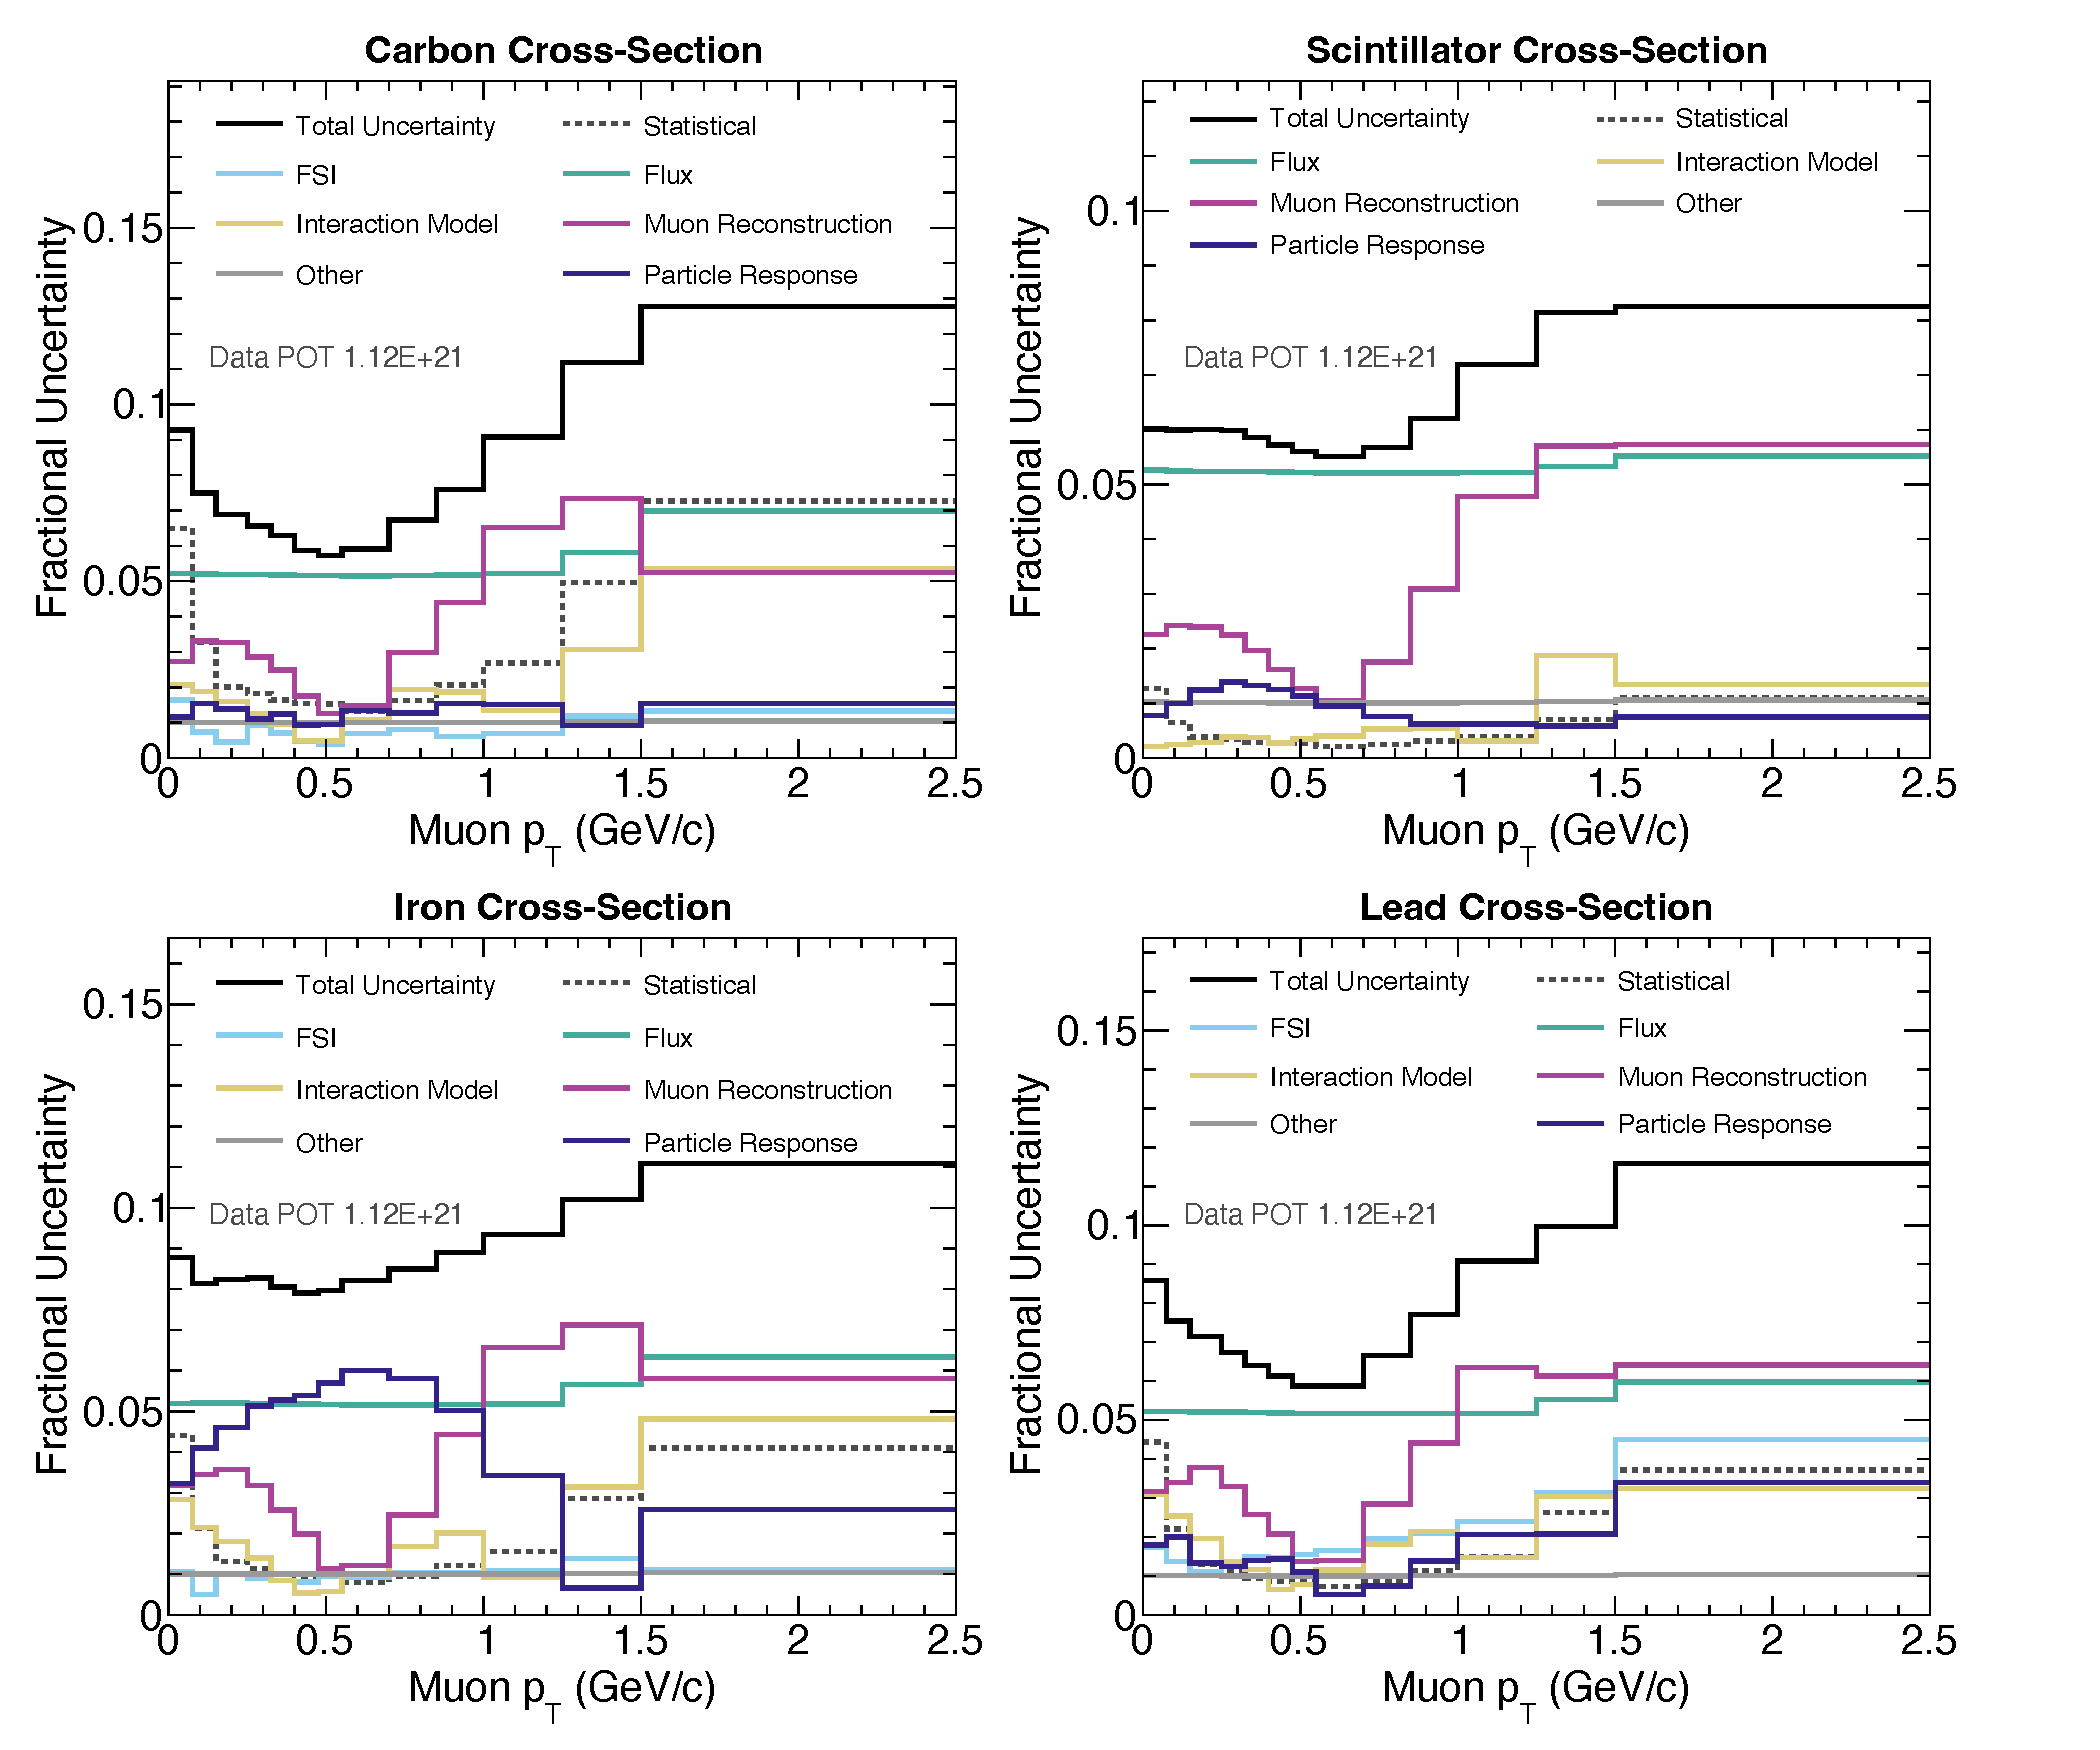
\includegraphics[width=1.\textwidth]{09results/figures/xsec_pT_fracErr.pdf}}%
    \caption{Breakdown of the fractional uncertainties on the data cross-section in $p_{\text{T}}$ for carbon, hydrocarbon, iron, and lead (from left to right, top to bottom). Note that the cross-sections are dominated by the uncertainties on flux and antimuon reconstruction.}
    \label{fig:xsec_pT_fracErr}
\end{figure}

An interesting observation is the flat carbon-to-scintillator ratio in Figure~\ref{fig:ratio_pT}, which does not completely agree with the simulation prediction at unity, contrary to expectations. However, it is important to note that the systematic uncertainties on the data are missing the uncertainty accounting for the discrepancy in the plastic sidebands after the normalisation tune discussed in Section~\ref{sec:bkgSubtraction} and Chapter~\ref{ch:systematics}. Given that the shape of the ratio somewhat mirrors the shape of the data-to-simulation ratio in the sideband, this is expected to account for the discrepancy between the data and the simulation prediction in the final carbon-to-scintillator cross-section ratio. Alternatively, this discrepancy is also expected to be mitigated if the plastic sideband procedure is improved, for example, by fitting in the three distinct regions of $p_{\text{T}}$ (low, peak, and high $p_{\text{T}}$) to remove the shape differences in the sideband rather than using a simple normalisation fit. 

\begin{figure}[t!] 
    \centering
    {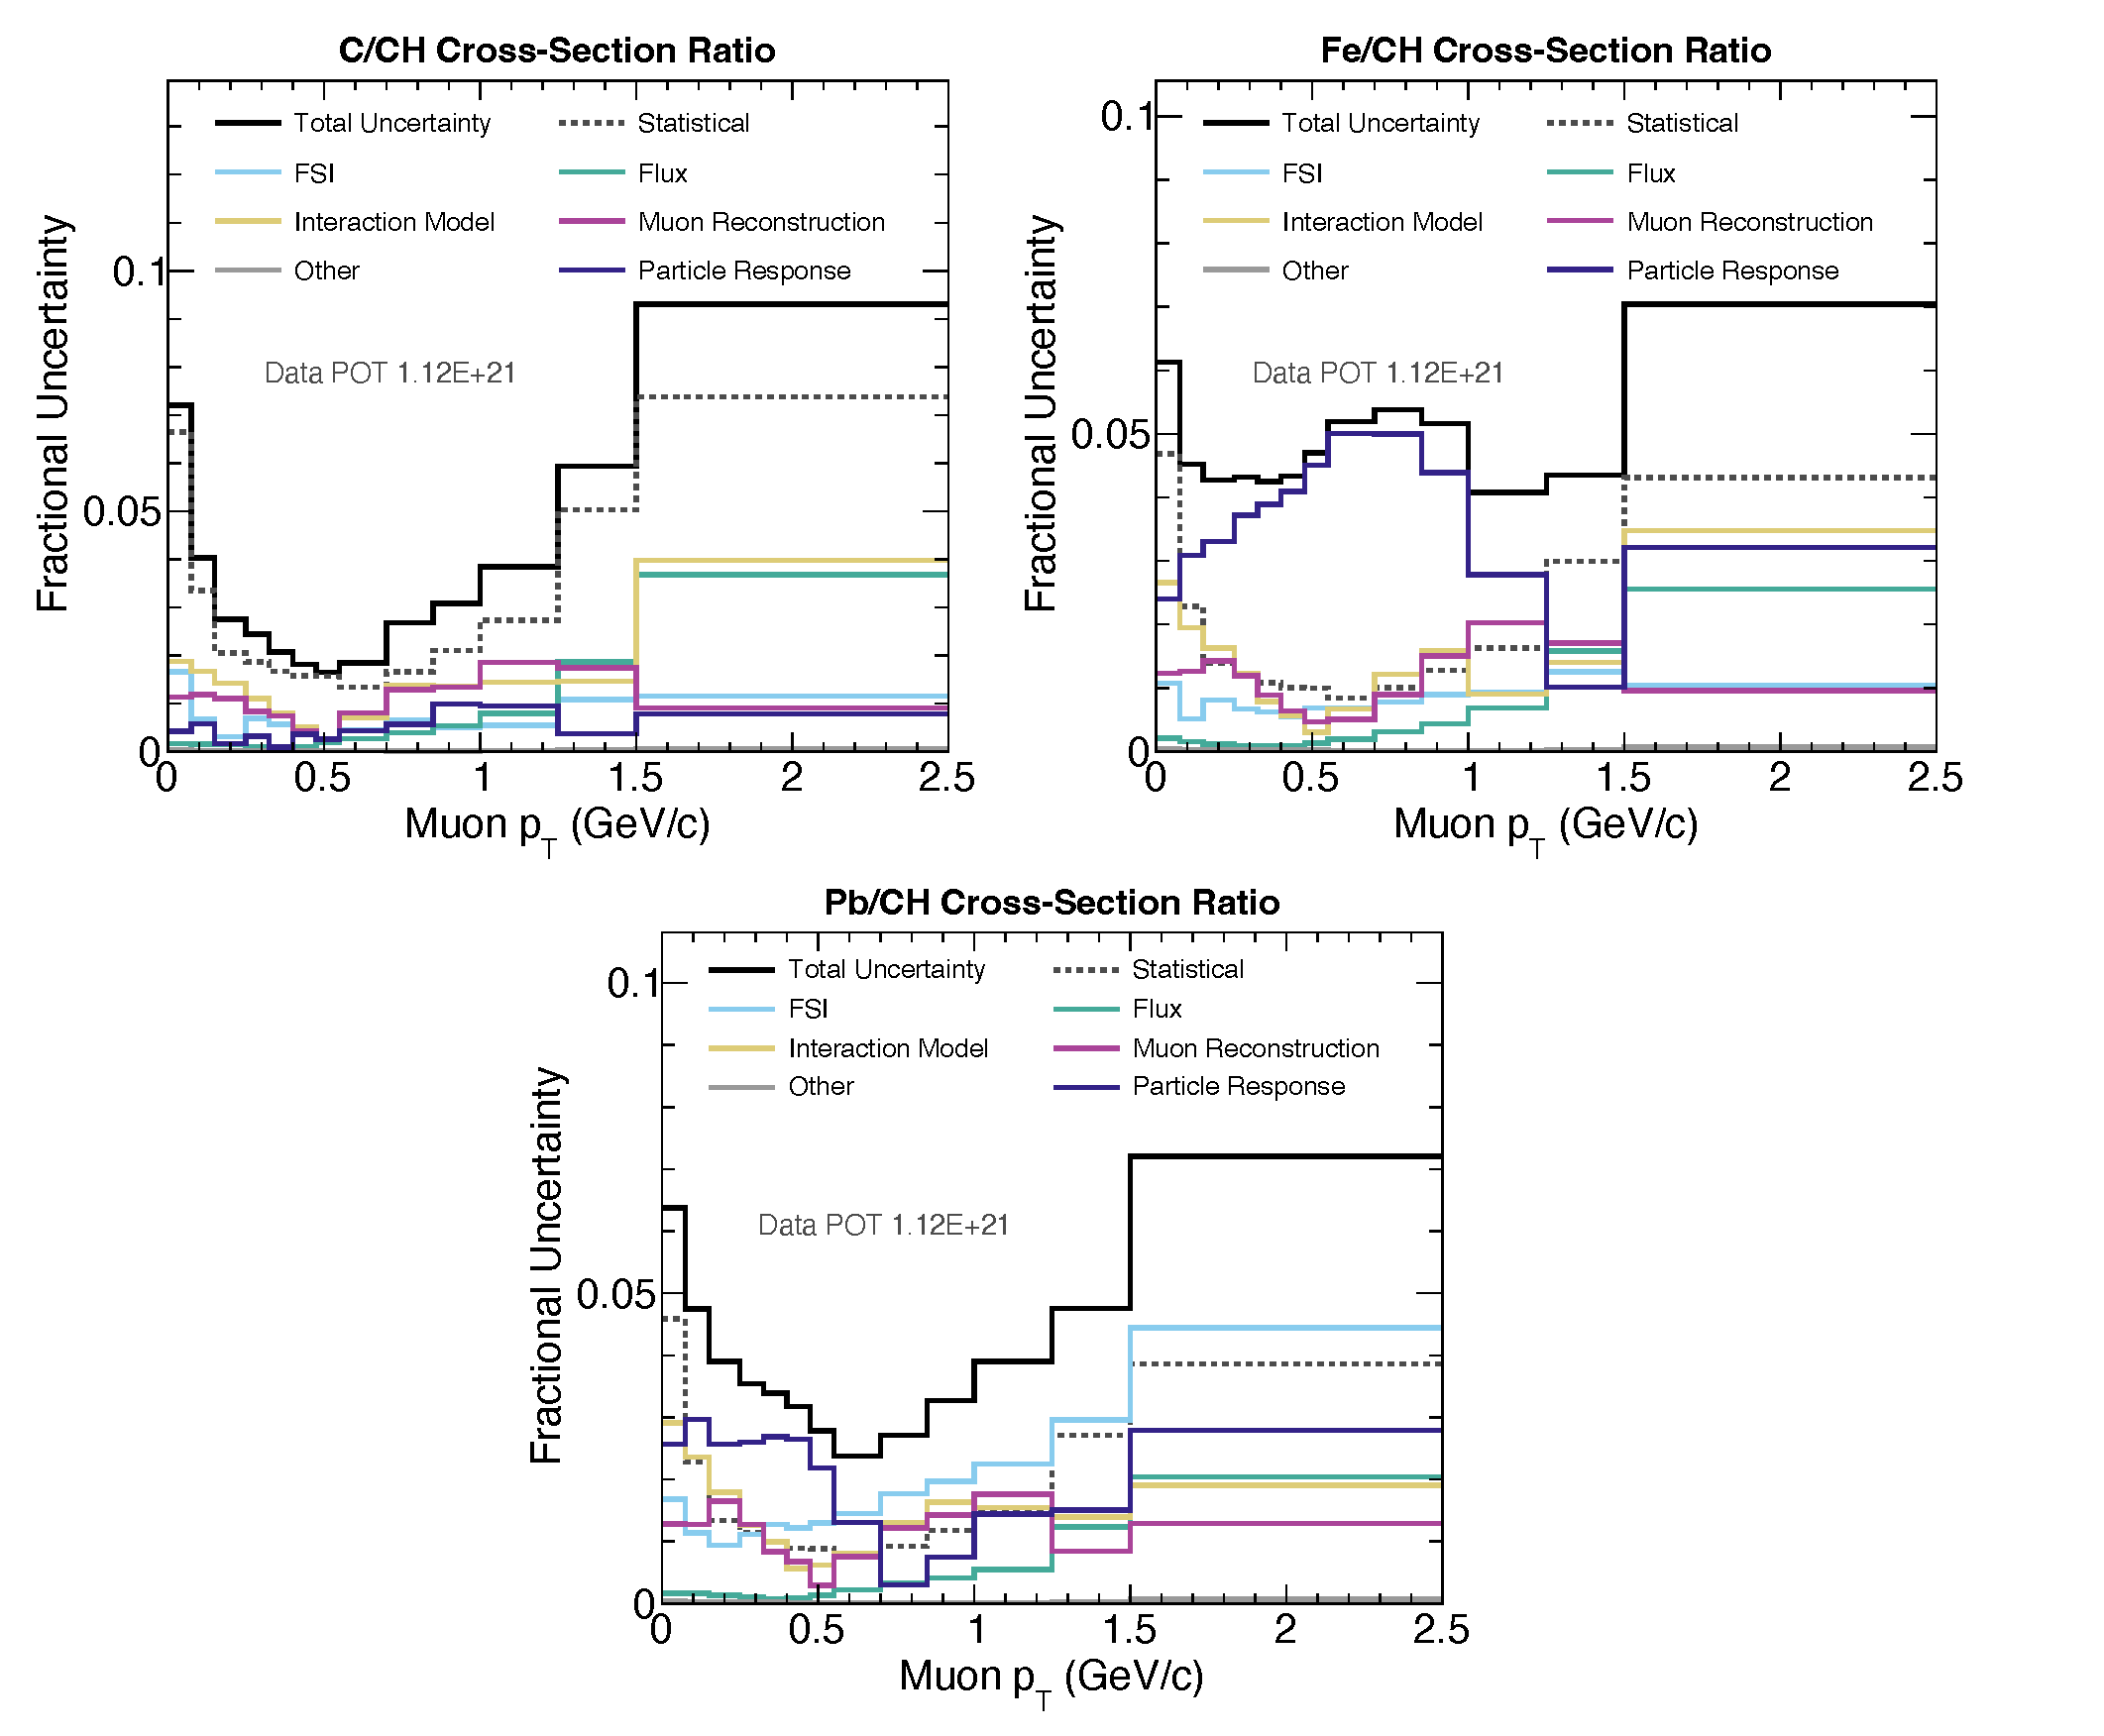
\includegraphics[width=1.\textwidth]{09results/figures/ratios_pT_fracErr.pdf}}%
    \caption{Breakdown of the fractional uncertainties on the data cross-section ratios to scintillator for carbon (top left), iron (top right), and lead (bottom) in antimuon $p_{\text{T}}$. Note that the flux and detector-related uncertainties are mostly cancelled out. A significant feature is the increase of the `FSI' error band going from light carbon to heavy lead. }
    \label{fig:ratio_pT_fracErr}
\end{figure}

Finally, the breakdowns of fractional uncertainties for both the cross-sections and cross-section ratios in $p_{\text{T}}$ are demonstrated in Figures~\ref{fig:xsec_pT_fracErr} and~\ref{fig:ratio_pT_fracErr}, respectively. The individual cross-sections are primarily influenced by systematic uncertainty rather than statistical uncertainty, specifically stemming from the flux and the antimuon reconstruction uncertainties. These two sources of uncertainty tend to cancel out to a large extent in the cross-section ratios, as evident in Figure~\ref{fig:ratio_pT_fracErr}. Consequently, the cross-section ratios become predominantly limited by statistical uncertainties.

When comparing C/CH, Fe/CH, and Pb/CH, a noticeable increase in the uncertainty on the final-state interaction~(`FSI') is observed as FSI becomes more significant and complex for heavier nuclei. It is important to note that the `Particle Response' uncertainty band is mainly driven by uncertainties in GEANT4 neutron interaction modelling, impacting the analysis due to correlations between outgoing particle kinematics (as $p_{\text{T}}$ serves as a proxy for the momentum transfer). A similar impact of the GEANT4 neutron modelling uncertainty in iron has been observed in other MINERvA analyses, such as in Ref.~\cite{Bercellie2023_PhysRevLett.131.011801}, and is currently under investigation, potentially arising from large weights in the neutron reweight described in Section~\ref{sec:particleProp}. %Note that the full covariance matrices for the measured antimuon $p_{\text{T}}$ cross-sections are included in Appendix~\ref{ch:appendix_covarianceMatrices}.
\clearpage
\section{Bjorken~$x$ results}


Figures~\ref{fig:xsec_x} and \ref{fig:ratio_x} show the results of the differential cross-sections and cross-section ratios for various nuclei as functions of the dimensionless scaling variable Bjorken $x$. As discussed in Chapter~\ref{ch:measurement}, Bjorken $x$ is used to describe nuclear modifications to a bound nucleon cross-section compared to a free nucleon. While this effect is primarily associated with deep inelastic scattering (DIS), the substantial DIS contribution in this analysis sample makes the investigation interesting. By definition, the DIS contribution is expected to be large at low $x$ (corresponding to large recoil energy), while the quasi-elastic contribution should dominate the high $x$ region. This is illustrated in the interaction breakdown of the simulation prediction cross-section in Figure~\ref{fig:xsec_x}.

\begin{figure}[t!] 
    \vspace{20pt}
    \centering
    {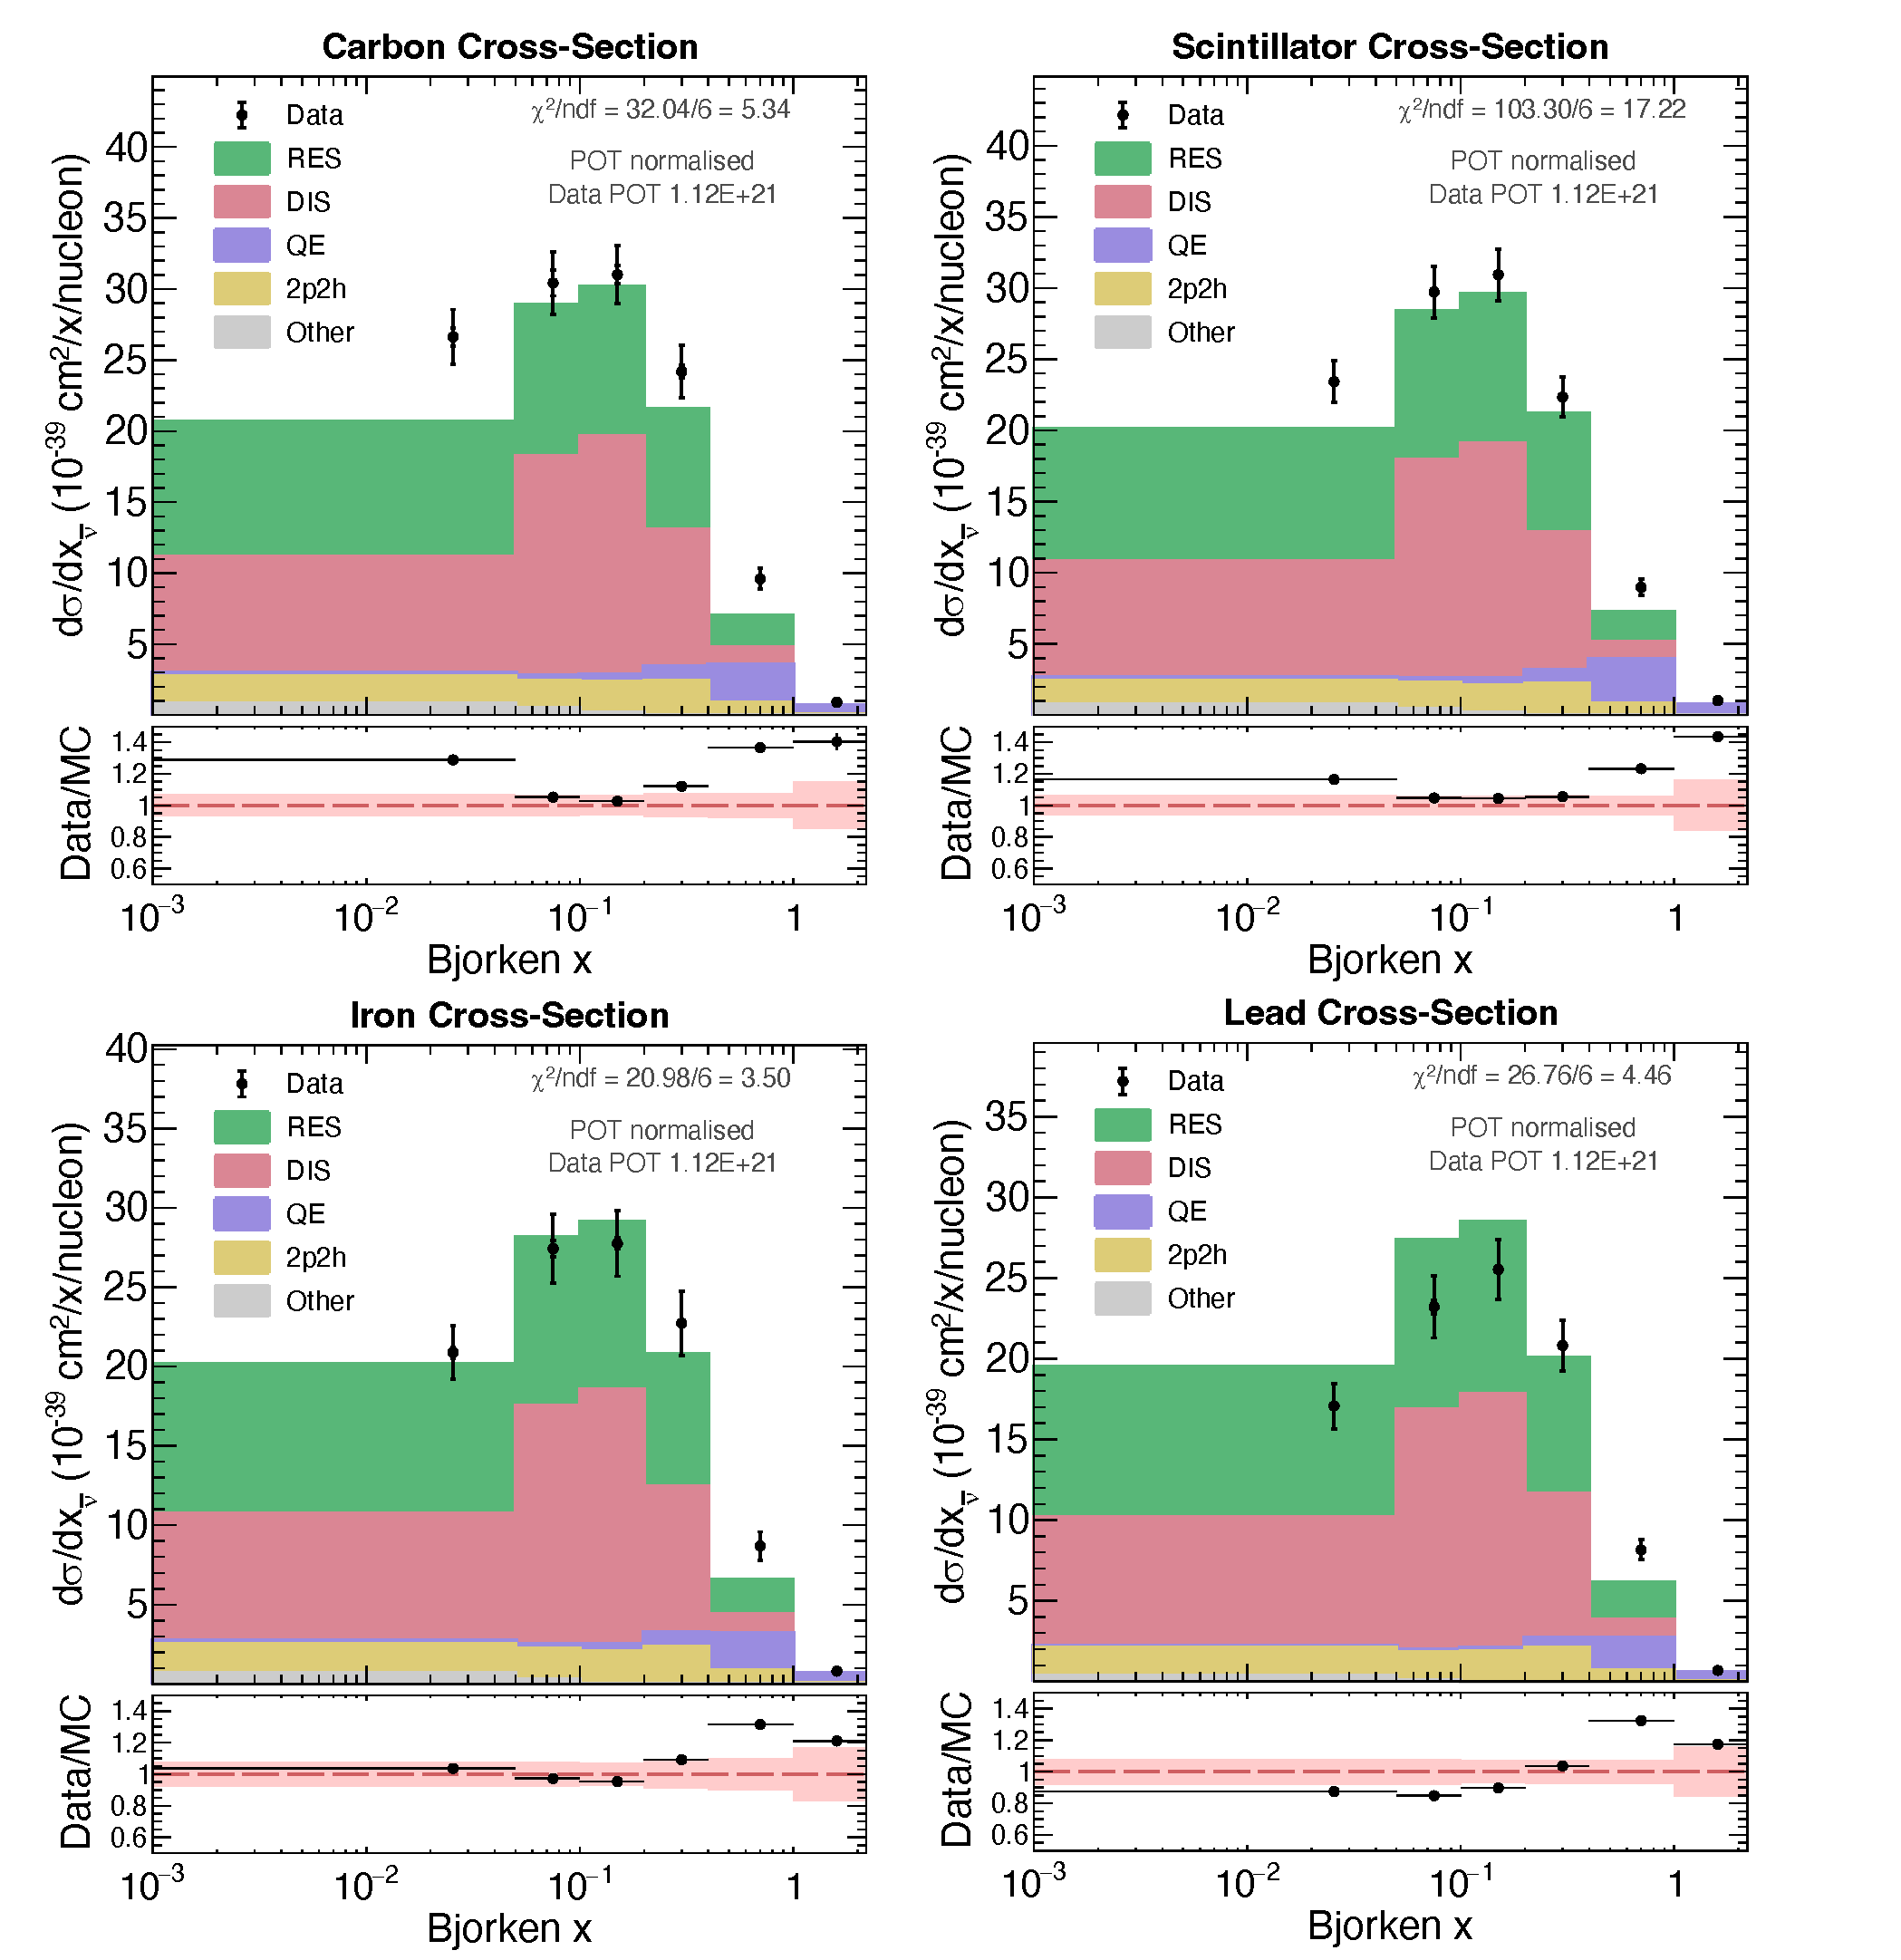
\includegraphics[width=1.\textwidth]{09results/figures/xsec_x.pdf}}%
    \caption{Carbon, scintillator, iron, and lead (from left to right, top to bottom) cross-section as a function of Bjorken $x$ with the simulation broken down into the various interaction channels stacked in the descending order of their contribution. In the top panel of each plot, the data points carry both statistical (inner error bar) and systematic (outer error bar, which is the sum of statistical and systematic errors) uncertainties. The bottom panel of each plot displays the data-to-simulation ratio, with the pink band around 1 representing systematic uncertainty on the data, while the black points reflect the statistical uncertainty on the data-to-simulation ratio.}
    \label{fig:xsec_x}
\end{figure}




\begin{figure}[t!] 
    \centering
    {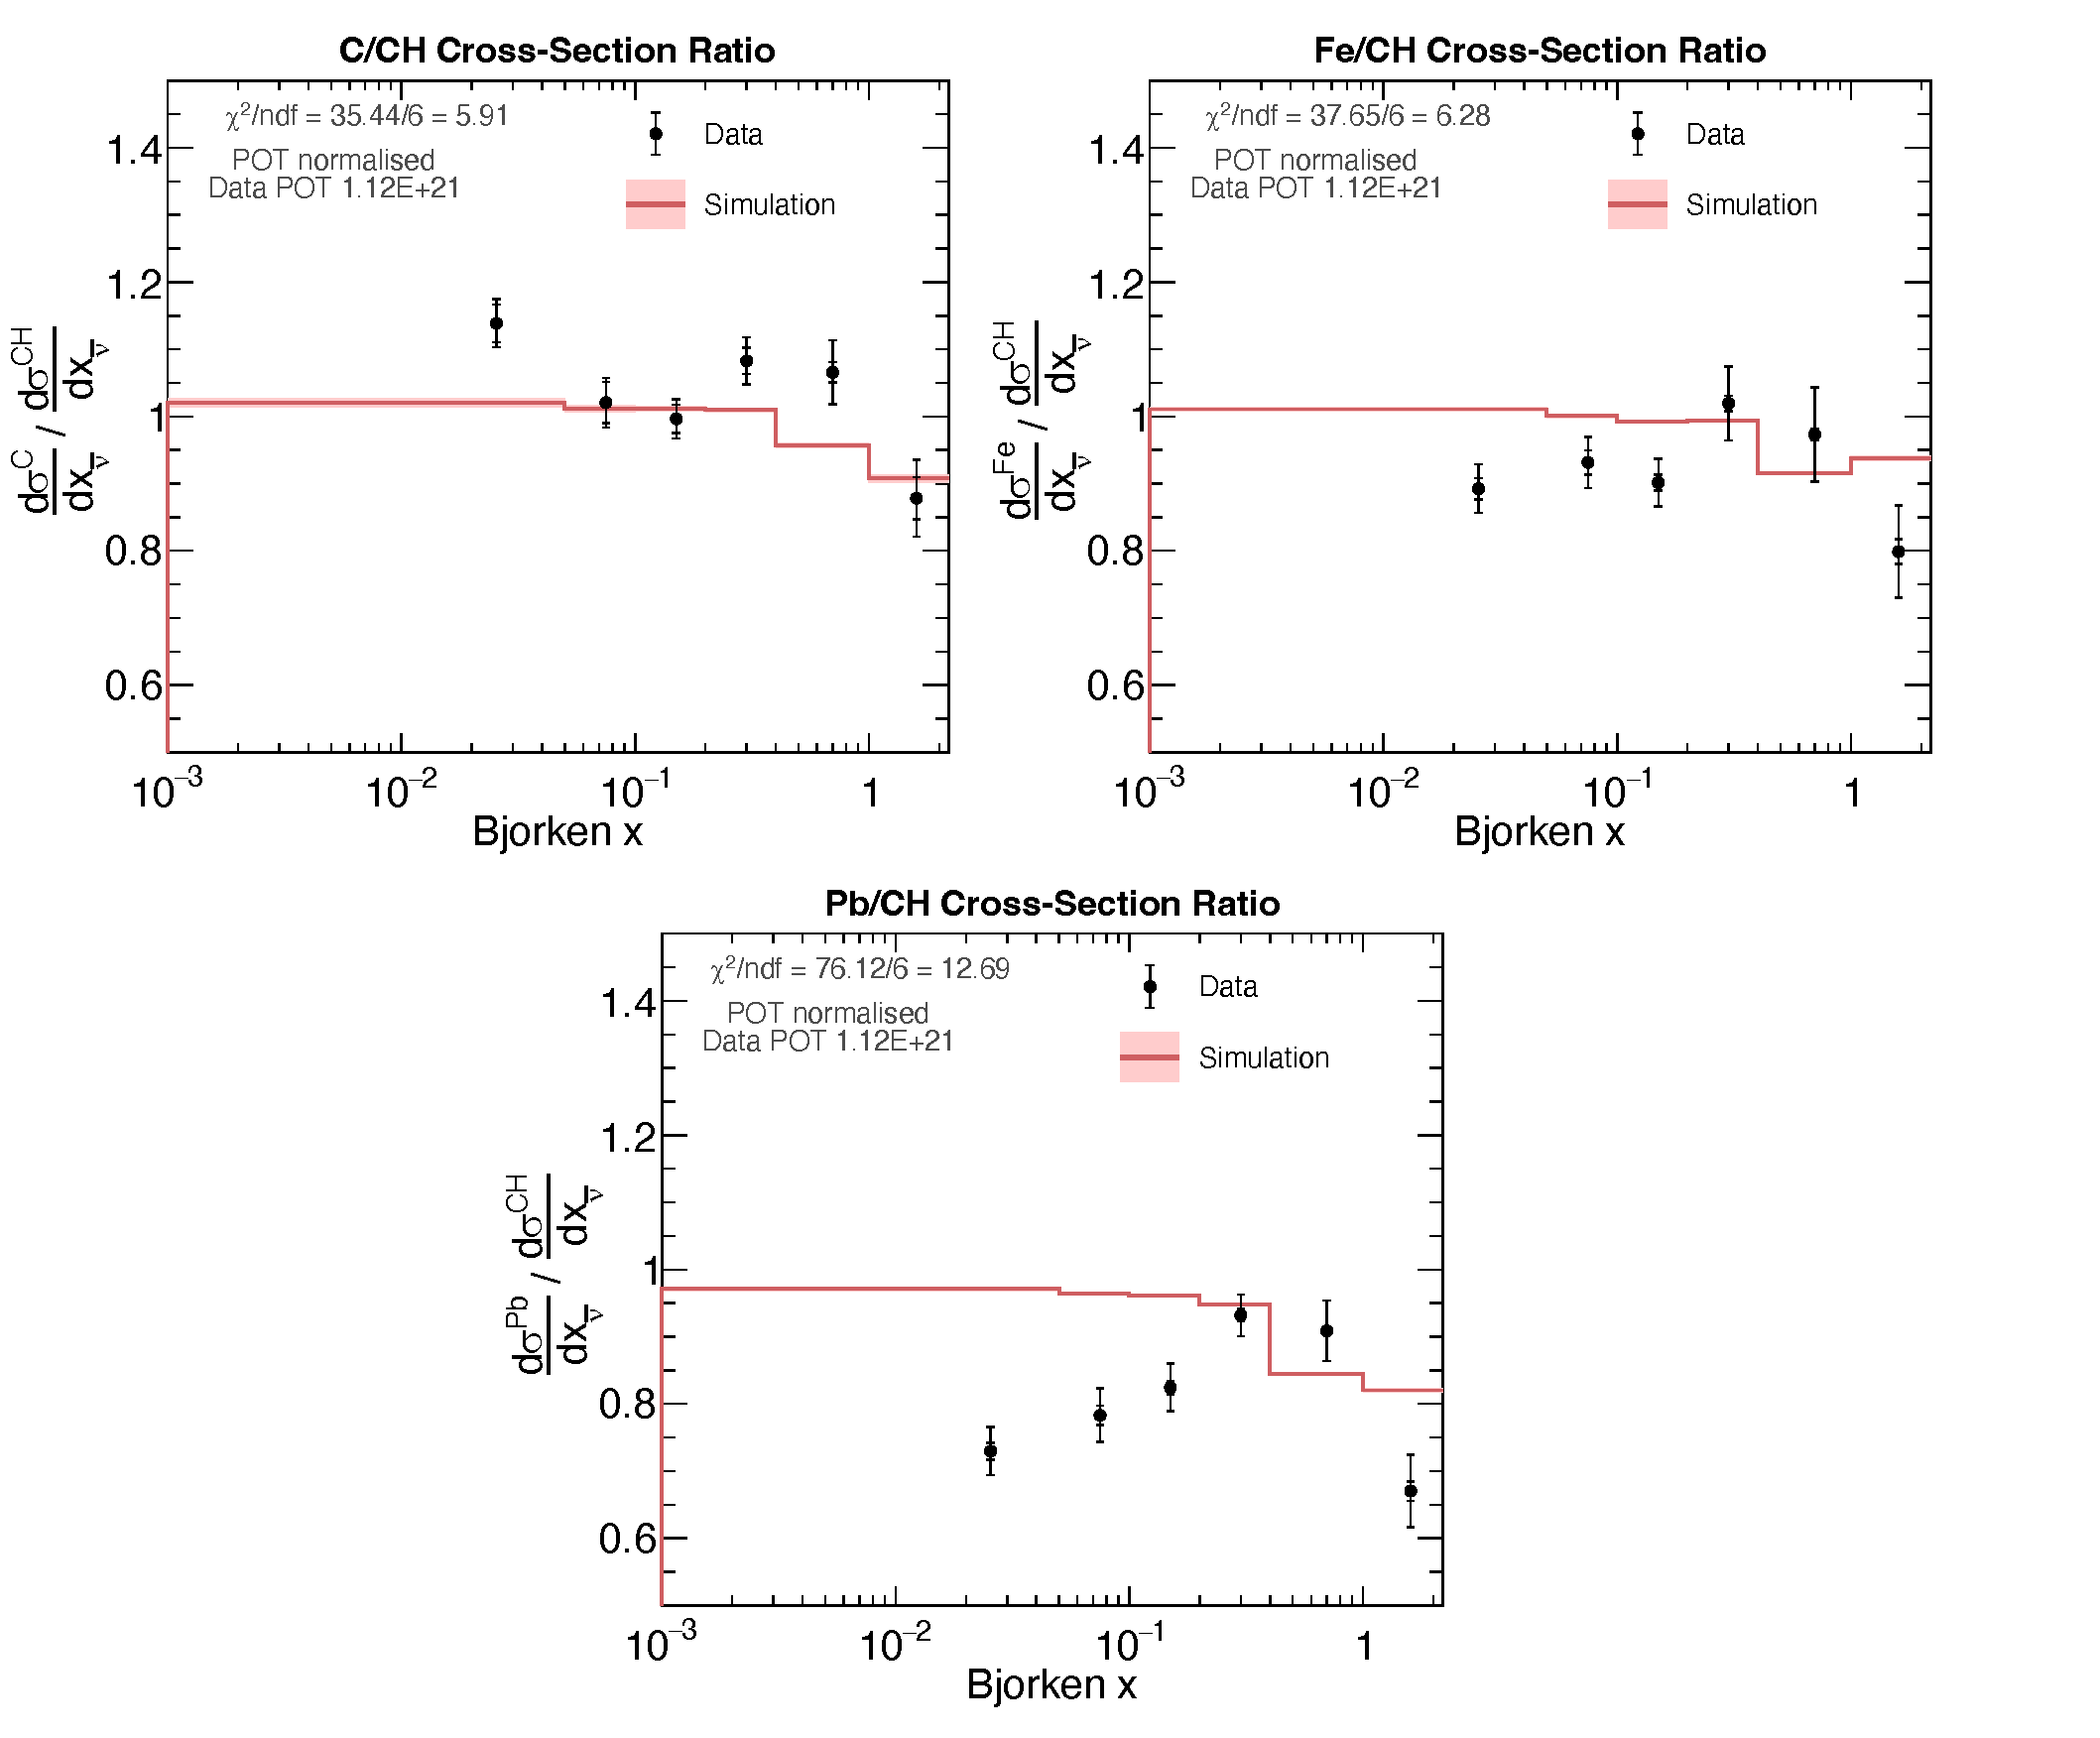
\includegraphics[width=1.\textwidth]{09results/figures/ratios_x.pdf}}%
    \caption{Carbon-to-scintillator (top left), iron-to-scintillator (top right), and lead-to-scintillator (bottom) cross-section ratios in Bjorken $x$. The data points carry both statistical (inner error bar) and systematic (outer error bar, which is the sum of statistical and systematic errors) uncertainties. The error band around the simulation predictions represents its statistical error. Note the $A$-dependent difference across the measured ratios, particularly in the low-Bjorken $x$ region.}
    \label{fig:ratio_x}
\end{figure}

The cross-section ratios for iron and lead in Bjorken $x$ in Figure~\ref{fig:ratio_x} exhibit significant disagreement with the underlying simulation in the low $x$ region. These ratios particularly demonstrate a notable suppression of the iron and lead cross-section in this region compared to the scintillator, and the suppression grows with the size of the nucleus. This is in agreement with MINERvA's first investigation of such effects in the low-energy inclusive neutrino scattering~\cite{Tice_PhysRevLett.112.231801}. Note that the results of this analysis represent the first comprehensive and statistically significant investigation of such effects across various nuclei in the medium-energy inclusive antineutrino sample. The low-energy equivalent was not possible due to limited statistics. Compared to the neutrino results in low energy in Ref.~\cite{Tice_PhysRevLett.112.231801}, this analysis was performed using roughly 10$\times$ more interactions in each nucleus.

The depletion in the cross-sections for heavy targets at low $x$, referred to as shadowing-like region, mainly due to the DIS contribution is generally expected, and it is attributed to the destructive interference of hadronic fluctuations of the intermediate boson that multiple-scatter off surface nucleons,~\cite{KOPELIOVICH2013314, BEBCWA59:1989nmi, Tice_PhysRevLett.112.231801}, as explained in Chapter~\ref{ch:measurement}. There are several reasons why the depletion may be larger in the data than predicted by the simulation. First, the shadowing corrections included in the simulation prediction are based on charged lepton data, which, unlike antineutrinos, do not have axial-vector contributions. Additionally, the same shadowing corrections based on iron data are also applied to carbon and lead \cite{BODEK2005113}, as mentioned in Chapter~\ref{ch:dataAsimulation}. Furthermore, more than 85\% of the data has $Q^2 < $ 1 (GeV/$c$)$^2$, whereas the underlying simulation is tuned to the perturbative region of higher $Q^2$ data.
%\enlargethispage{1\baselineskip}


Importantly, interpreting the observed suppression of heavy target cross-sections at low $x$ is challenging, as it is impossible to disentangle FSI and nuclear effects due to the inclusive nature of the analysis. FSI effects may distort the observed Bjorken $x$ distribution by increasing or decreasing the observed recoil energy, with such effects possibly more pronounced in heavier nuclei, introducing strong nuclear dependence effects. Additional complexity also arises due to the interplay between pion production and deep inelastic scattering in the low $x$ region, which may be resolved with MINERvA's incoming deep and shallow inelastic scattering results. 

The high-$x$ region, dominated by quasi-elastic scattering across various nuclei, is also overpredicted in the cross-section ratios for iron and lead. However, its interpretation is also somewhat complex. The corresponding migration matrices in Section~\ref{sec:migration_unfolding} showed large smearing in this region, and while the model dependence in unfolding was studied, the quasi-elastic scattering in antineutrino interactions results in neutrons, which are often invisible to the calorimetric recoil reconstruction. The correction to the recoil energy accounting for this is inherently model-dependent as described in Chapter~\ref{ch:Reconstruction}.

\begin{figure}[t!] 
    \centering
    {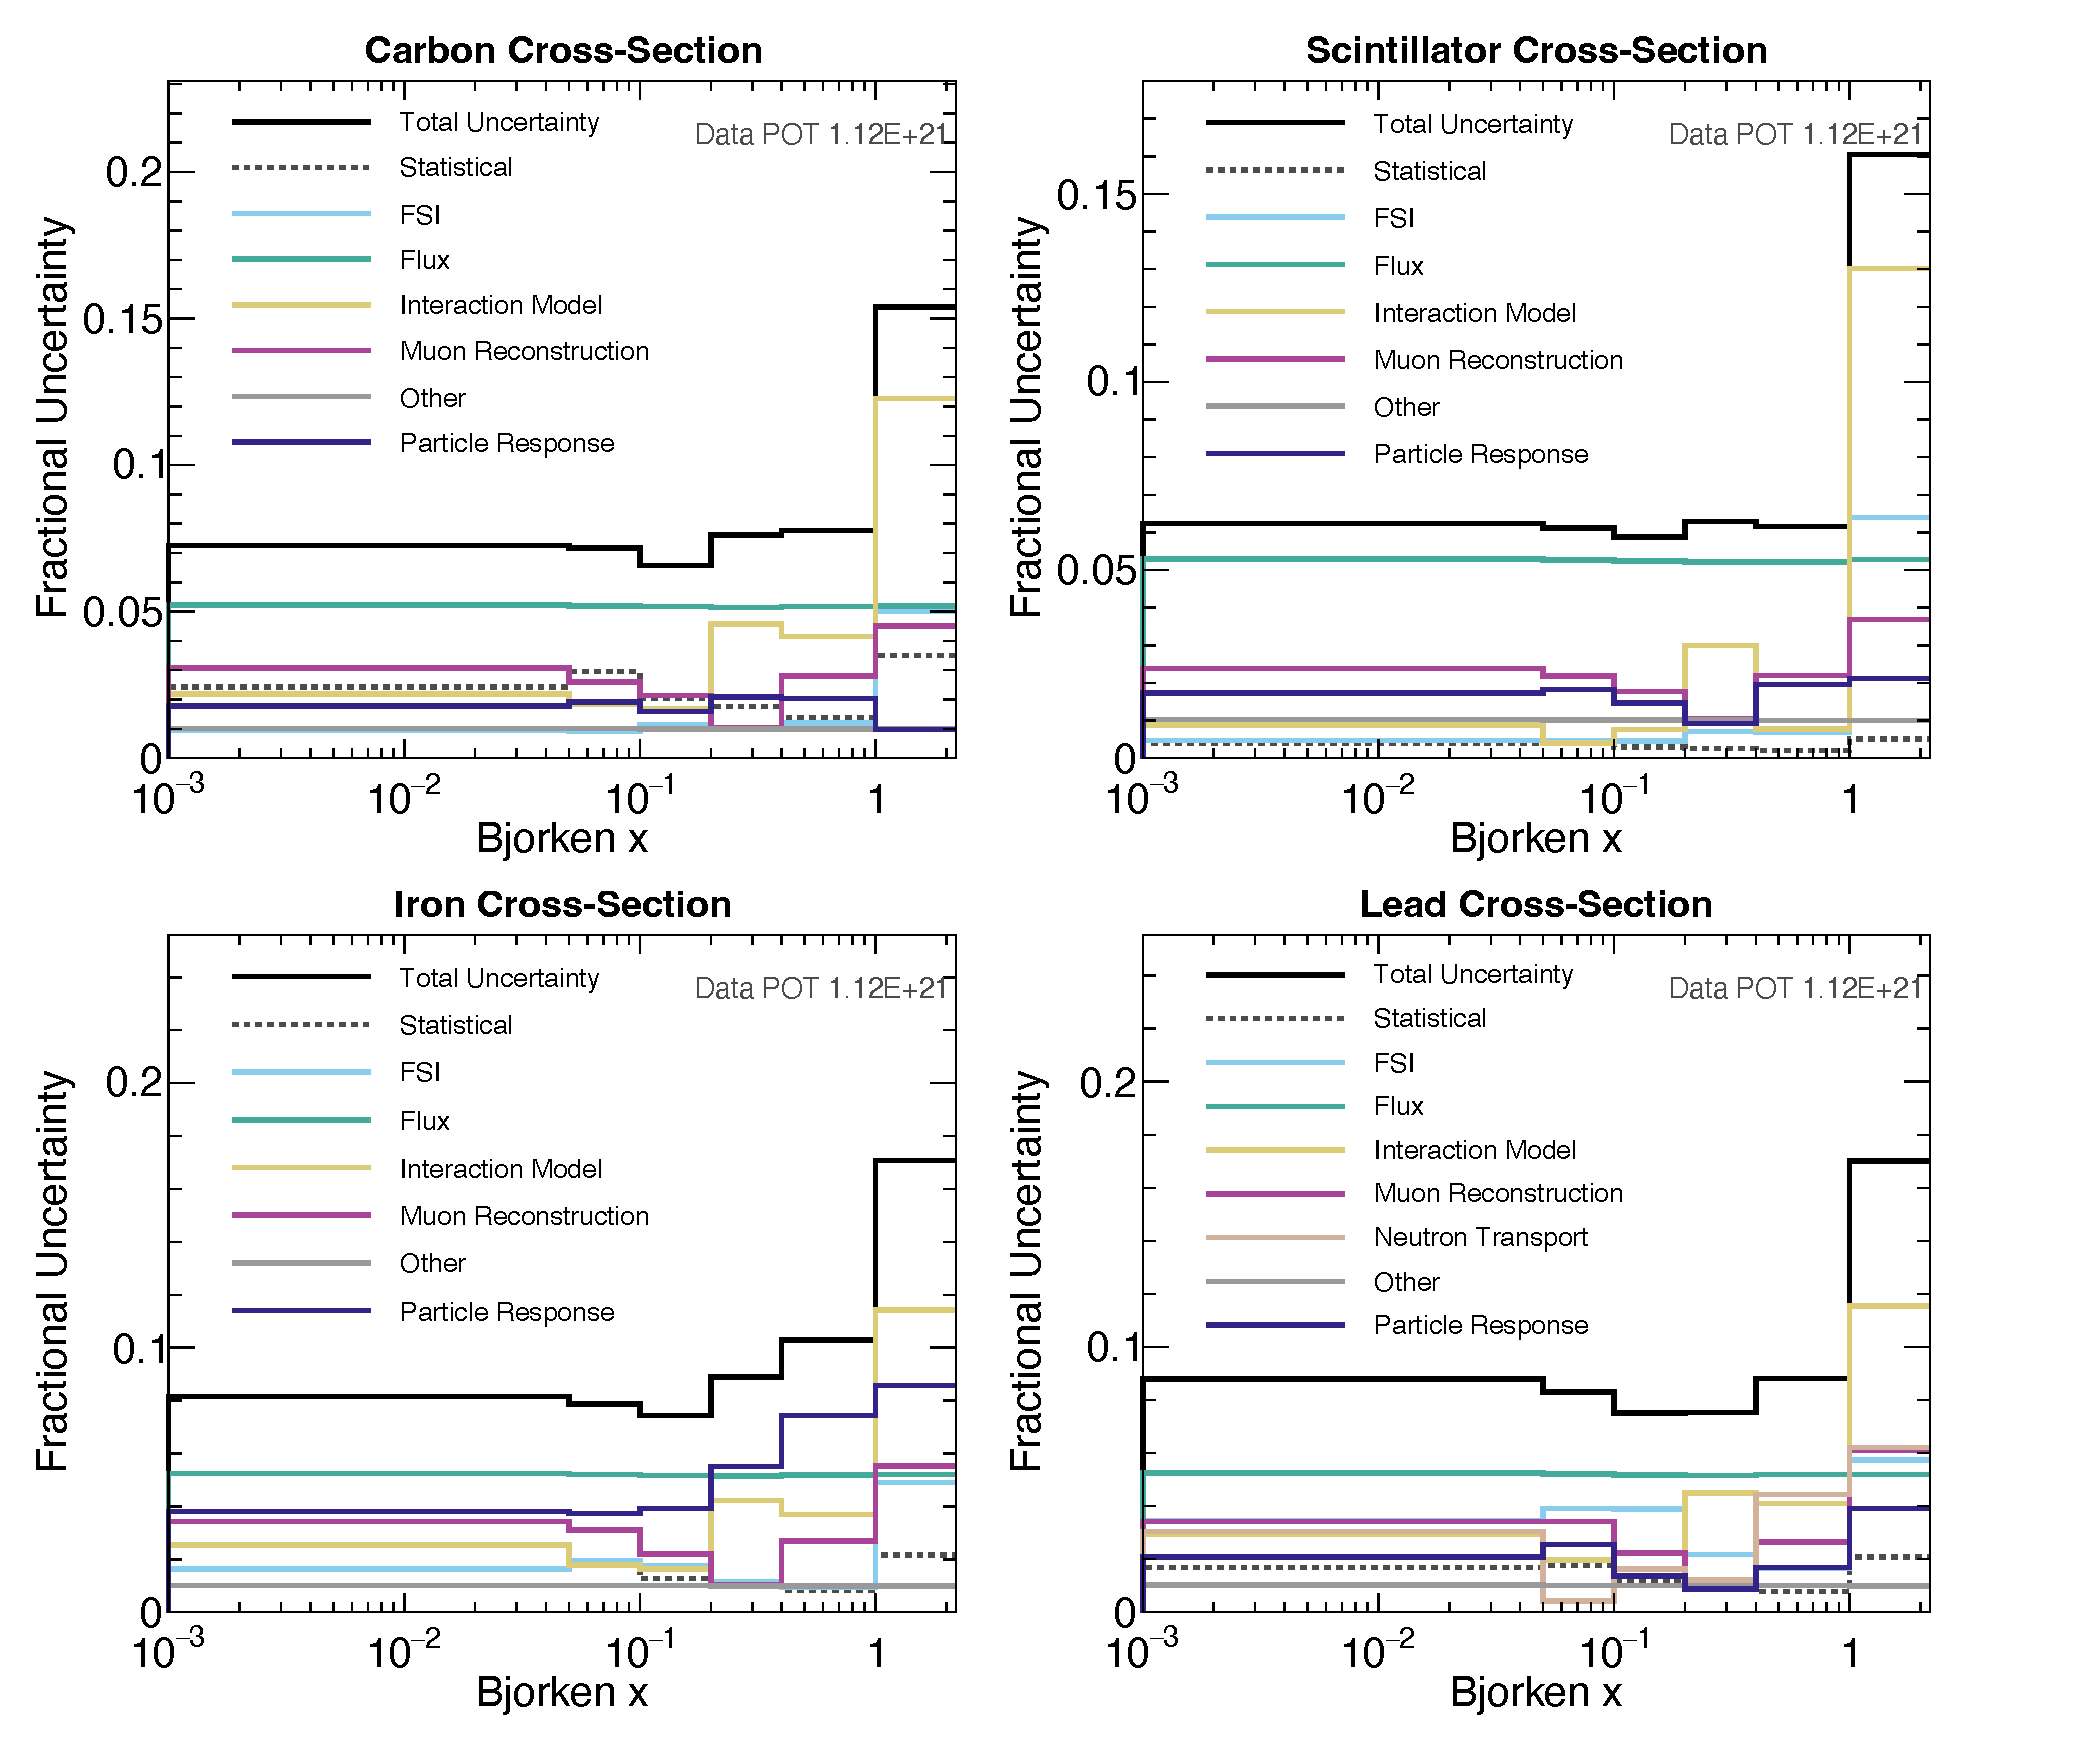
\includegraphics[width=1.\textwidth]{09results/figures/xsec_x_fracErr.pdf}}%
    \caption{Breakdown of the fractional uncertainties on the data cross-section in Bjorken~$x$ for carbon, hydrocarbon, iron, and lead (from left to right, top to bottom). Note that, in general, the cross-sections are dominated by uncertainties on flux, with the exception of the high-$x$ region, which is dominated by uncertainties on the underlying interaction model.}
    \label{fig:xsec_x_fracErr}
\end{figure}

Furthermore, the $x > 1$ region simulated by GENIE comes mostly from smearing from final-state interactions and does not include predictions of interactions from short-range correlated nucleons. These are expected to occur in this region based on electron-scattering data~\cite{CLAS:PhysRevLett.96.082501, SRC:annurev}. Also, the exploratory study of the potential bias due to neutron modelling corrections in Section~\ref{sec:migration_unfolding} suggested a need for additional uncertainty in this region, as discussed in Chapter~\ref{ch:systematics}. Nevertheless, this analysis presents the first attempt to measure this region in antineutrino scattering and the data seems to indicate the need for a larger suppression at high $x$ compared to carbon. However, the challenges described above preclude the analysis from making any definitive conclusions. 

\begin{figure}[t!] 
    \centering
    {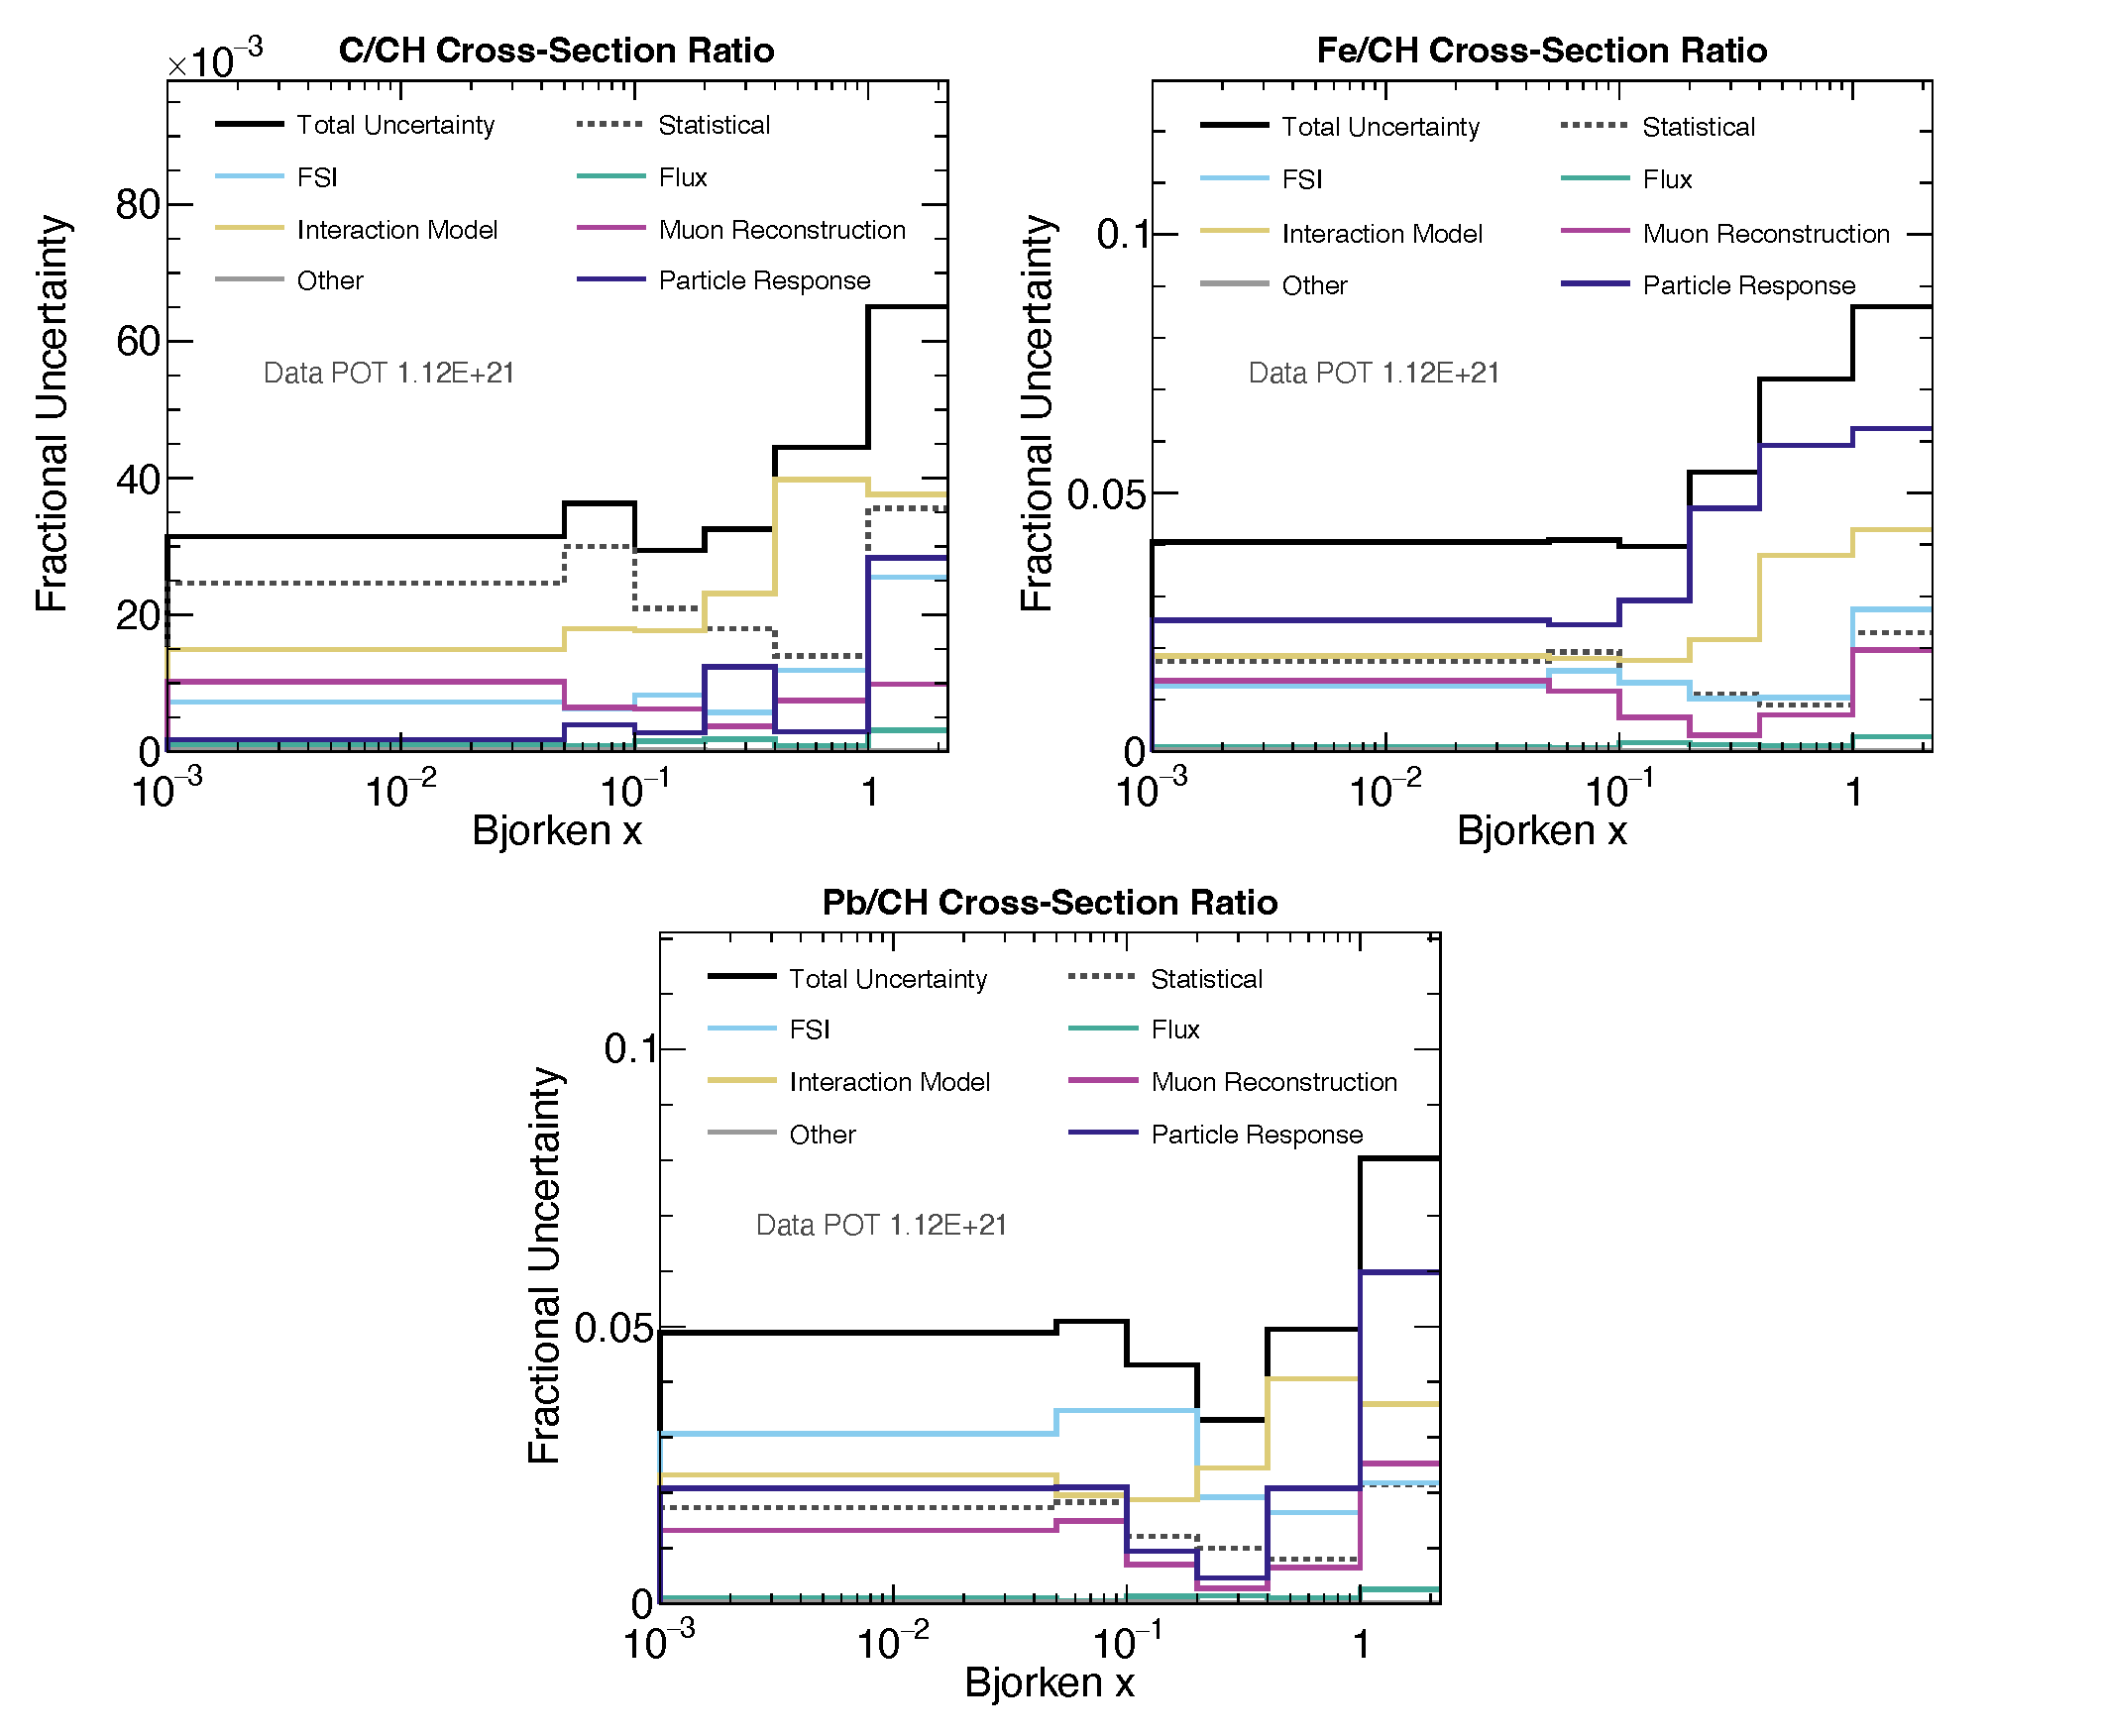
\includegraphics[width=1.\textwidth]{09results/figures/ratios_x_fracErr.pdf}}%
    \caption{Breakdown of the fractional uncertainties on the data cross-section ratios to scintillator for carbon (top left), iron (top right), and lead (bottom) in Bjorken~$x$. Note that the flux and detector-related uncertainties are mostly cancelled out.}
    \label{fig:ratio_x_fracErr}
\end{figure}

Similarly to $p_{\text{T}}$, the carbon-to-scintillator ratio is most consistent with the simulation and with unity. The sideband effects discussed above for $p_{\text{T}}$ could potentially explain the differences from the underlying prediction of the ratio. Moreover, the low-$x$ region is also sensitive to the recoil energy scale, prompting a potential investigation into whether the recoil scale differs between the nuclear target region and the scintillator tracker.


Figures~\ref{fig:xsec_x_fracErr} and \ref{fig:ratio_x_fracErr} summarise the breakdowns of the fractional uncertainties on the Bjorken $x$ cross-sections and the cross-section ratios for various nuclei. Similar to the~$p_{\text{T}}$ cross-section, the Bjorken $x$ cross-section is dominated by flux uncertainty. The $x > 1$ region is governed by the understanding of the underlying interactions, i.e. `Interaction Model' error band, for the reasons described above. The C/CH ratio is mostly limited by the underlying statistics (except at large $x$). 

Overall, in all ratios, the `Interaction Model' error band represents the leading source of systematic uncertainty. Akin to the $p_{\text{T}}$ results, the contribution in iron from the `Particle Response' uncertainty band, i.e. GEANT4 neutron modelling, is being investigated. However, the `Particle Response' in this case also includes the calorimetric detector response, as Bjorken $x$ depends on recoil reconstruction, making its contribution overall larger than in $p_{\text{T}}$. Finally, the `FSI' uncertainty becomes more prominent in the ratio as the nucleus in the numerator gets heavier. %Similar to the $p_{\text{T}}$ cross-section results, the full covariance matrices for the measured Bjorken $x$ cross-sections are included in Appendix~\ref{ch:appendix_covarianceMatrices}.


\section{Model comparisons}


It is important to review the measured results in the context of other (anti)neutrino event generators that implement different interaction models than the underlying simulation used in the analysis. The different generator-to-data comparisons might give some insight into various aspects of the models, especially when extended to larger $A$, inform the neutrino interaction community, and potentially lead to further developments. Both the cross-sections and cross-section ratios are compared with a newer version of \mbox{GENIE~\cite{genie_ANDREOPOULOS201087,genie_andreopoulos2015}}, and a different event generator called NEUT~\cite{Hayato:2009zz, HayatoPickering2021}, which is primarily used in (anti)neutrino oscillation analyses at the T2K experiment~\cite{t2k_ABE2011106}.

Various aspects of the different generators that are relevant to the analysis and in which they differ from the underlying simulation (outlined in Chapter~\ref{ch:dataAsimulation}) are briefly described below.

\vspace{5pt}
% https://genie-docdb.pp.rl.ac.uk/DocDB/0000/000002/003/man.pdf
\noindent \textbf{GENIE version 3.0.6} \cite{genie3}: The resonant pion production is simulated by the Berger-Sehgal model~\cite{PhysRevD.76.113004} instead of the Rein-Sehgal\cite{REIN198179}. The Berger-Sehgal update includes effects due to the muon mass in the cross-section calculation~\cite{kuzmin, coherentMass_REIN2007207,Adler_2006}, and new implementation \cite{Nowak_2009} of different axial and vector form factors~\cite{PhysRevD.77.053001}. The parameters of the vector form factor are determined from electron scattering data \cite{PhysRevD.74.014009}. Furthermore, the FSI model is improved by emphasizing medium correlations between nucleons which suppress multiple scattering and have a strong $A$-dependence~\cite{genie3, PhysRevD.104.053006}.~There are two FSI models available, effective cascade $hA$ and full intranuclear cascade model $hN$. In addition, the differences between the individual labels in the model comparisons are:
% pion pole term which reproduce the expected Adler-screening effect at low $Q^2$ (because of the muon mass)
% diffractive model Rein and hyperon production using the pais model
% coherent pion production simulated by berger-seghal too
% used new implementation of axial and vector form factors based on Rarita-Schwinger 
% GENIE3 narrative
% https://indico.cern.ch/event/1175720/attachments/2470263/4237838/Resonances-20220627.pdf

\begin{itemize}
    \item GENIE3 G18\_02a/b uses the empirical 2p2h model \cite{genie_ANDREOPOULOS201087,katori2013meson}. The `a/b' tag represents the $hA$ and $hN$ FSI model, respectively. The label is a shorthand for the official GENIE 3 release G18\_02a/b\_02\_11a. 
    \item GENIE3 G18\_10a/b employs the local Fermi gas nuclear model \cite{RPANieves2004_PhysRevC.70.055503} instead of the relativistic Fermi gas \cite{RFG_SMITH1972605, 1975547}, and the quasi-elastic and 2p2h interactions are based on the Valencia model \cite{2p2hNieves2011_PhysRevC.83.045501}. Again `a' refers to $hA$ and `b' to $hN$ FSI model. The label is a shorthand for the official GENIE 3 release G18\_10a/b\_02\_11a. 
\end{itemize}

\vspace{5pt}
\noindent 
\textbf{NEUT version 5.4.1} \cite{Hayato:2009zz, HayatoPickering2021}: The resonant pion production is
simulated by the Berger-Sehgal~\cite{PhysRevD.76.113004}. A custom multi-pion-production model is used for $W < 2$ GeV$/c^2$, while deep inelastic scattering with $W > 2$ GeV$/c^2$ is simulated using PYTHIA/JETSET~\cite{Pythia_Sjostrand_2001}. Both are based on the Bodek-Yang model\cite{BodekYang_2003,BODEK2005113} parton distribution functions. The 2p2h interaction is simulated using the Valencia model \cite{2p2hNieves2011_PhysRevC.83.045501}. FSI uses a custom intranuclear cascade model. The two different labels have further distinguishing features:
%- developed for (anti)neutrino interactions on carbon and water, mostly for measurements of lepton kinematics
%- coherent Berger-Sehgal
%- diffractive Rein model
\begin{itemize}
    \item NEUT LFG ma105 uses the local Fermi gas nuclear model \cite{RPANieves2004_PhysRevC.70.055503} and the quasi-elastic scattering is based on the Valencia model \cite{2p2hNieves2011_PhysRevC.83.045501, Bourguille_2021} with $M_{A} = 1.05$ GeV$/c^2$.
    \item NEUT SF ma103 utilises the spectral function for the nuclear ground state with the associated quasi-elastic scattering \cite{Benhar:1994hw, Juszczak_2006, Furmanski:2015knr} with $M_{A} = 1.03$ GeV$/c^2$.
\end{itemize}
% what does it do for lead?
\noindent Note that the general differences between the various theoretical models were addressed in Chapter~\ref{ch:theory}.

% chi-squared statistic with general covariance matrix
In addition to the visual comparison, the agreement between the measured data and the various models is calculated using $\chi^2$, which takes into account bin-to-bin correlations,
\begin{equation}
    \chi^2 = \sum_{ij} (x_i - \mu_i) \text{cov}_{ij}^{-1} (x_j - \mu_j) \hspace{2pt} .
    \label{eq:fullyCorrelatedChi2}
\end{equation}
The $\text{cov}_{ij}$ represents the element of the covariance matrix defined in Chapter~\ref{ch:systematics}, $x_i$ is the data in bin $i$, and $\mu_i$ is the corresponding model prediction. Note that the $\chi^2$ differences in the inclusive sample are often small as some model changes do not have large impact on the inclusive cross-section.

Figures~\ref{fig:xsec_pT_modelComparison} and \ref{fig:ratio_pT_modelComparison} show the $p_{\text{T}}$ cross-section and cross-section ratio model comparisons, respectively, across the different nuclei. The corresponding fully-correlated $\chi^2$s per degree of freedom (the number of bins) are summarised in Tables~\ref{table:xsec_modelComparison_pT} and~\ref{table:xsecRatio_modelComparison_pT}.
The Bjorken $x$ results are compared to other models in Figures \ref{fig:xsec_x_modelComparison} and \ref{fig:ratio_x_modelComparison} with the corresponding $\chi^2$s presented in Tables~\ref{table:xsec_modelComparison_x} and~\ref{table:xsecRatio_modelComparison_x}, respectively.

\begin{figure}[t!] 
    \vspace{30pt}
    \centering
    {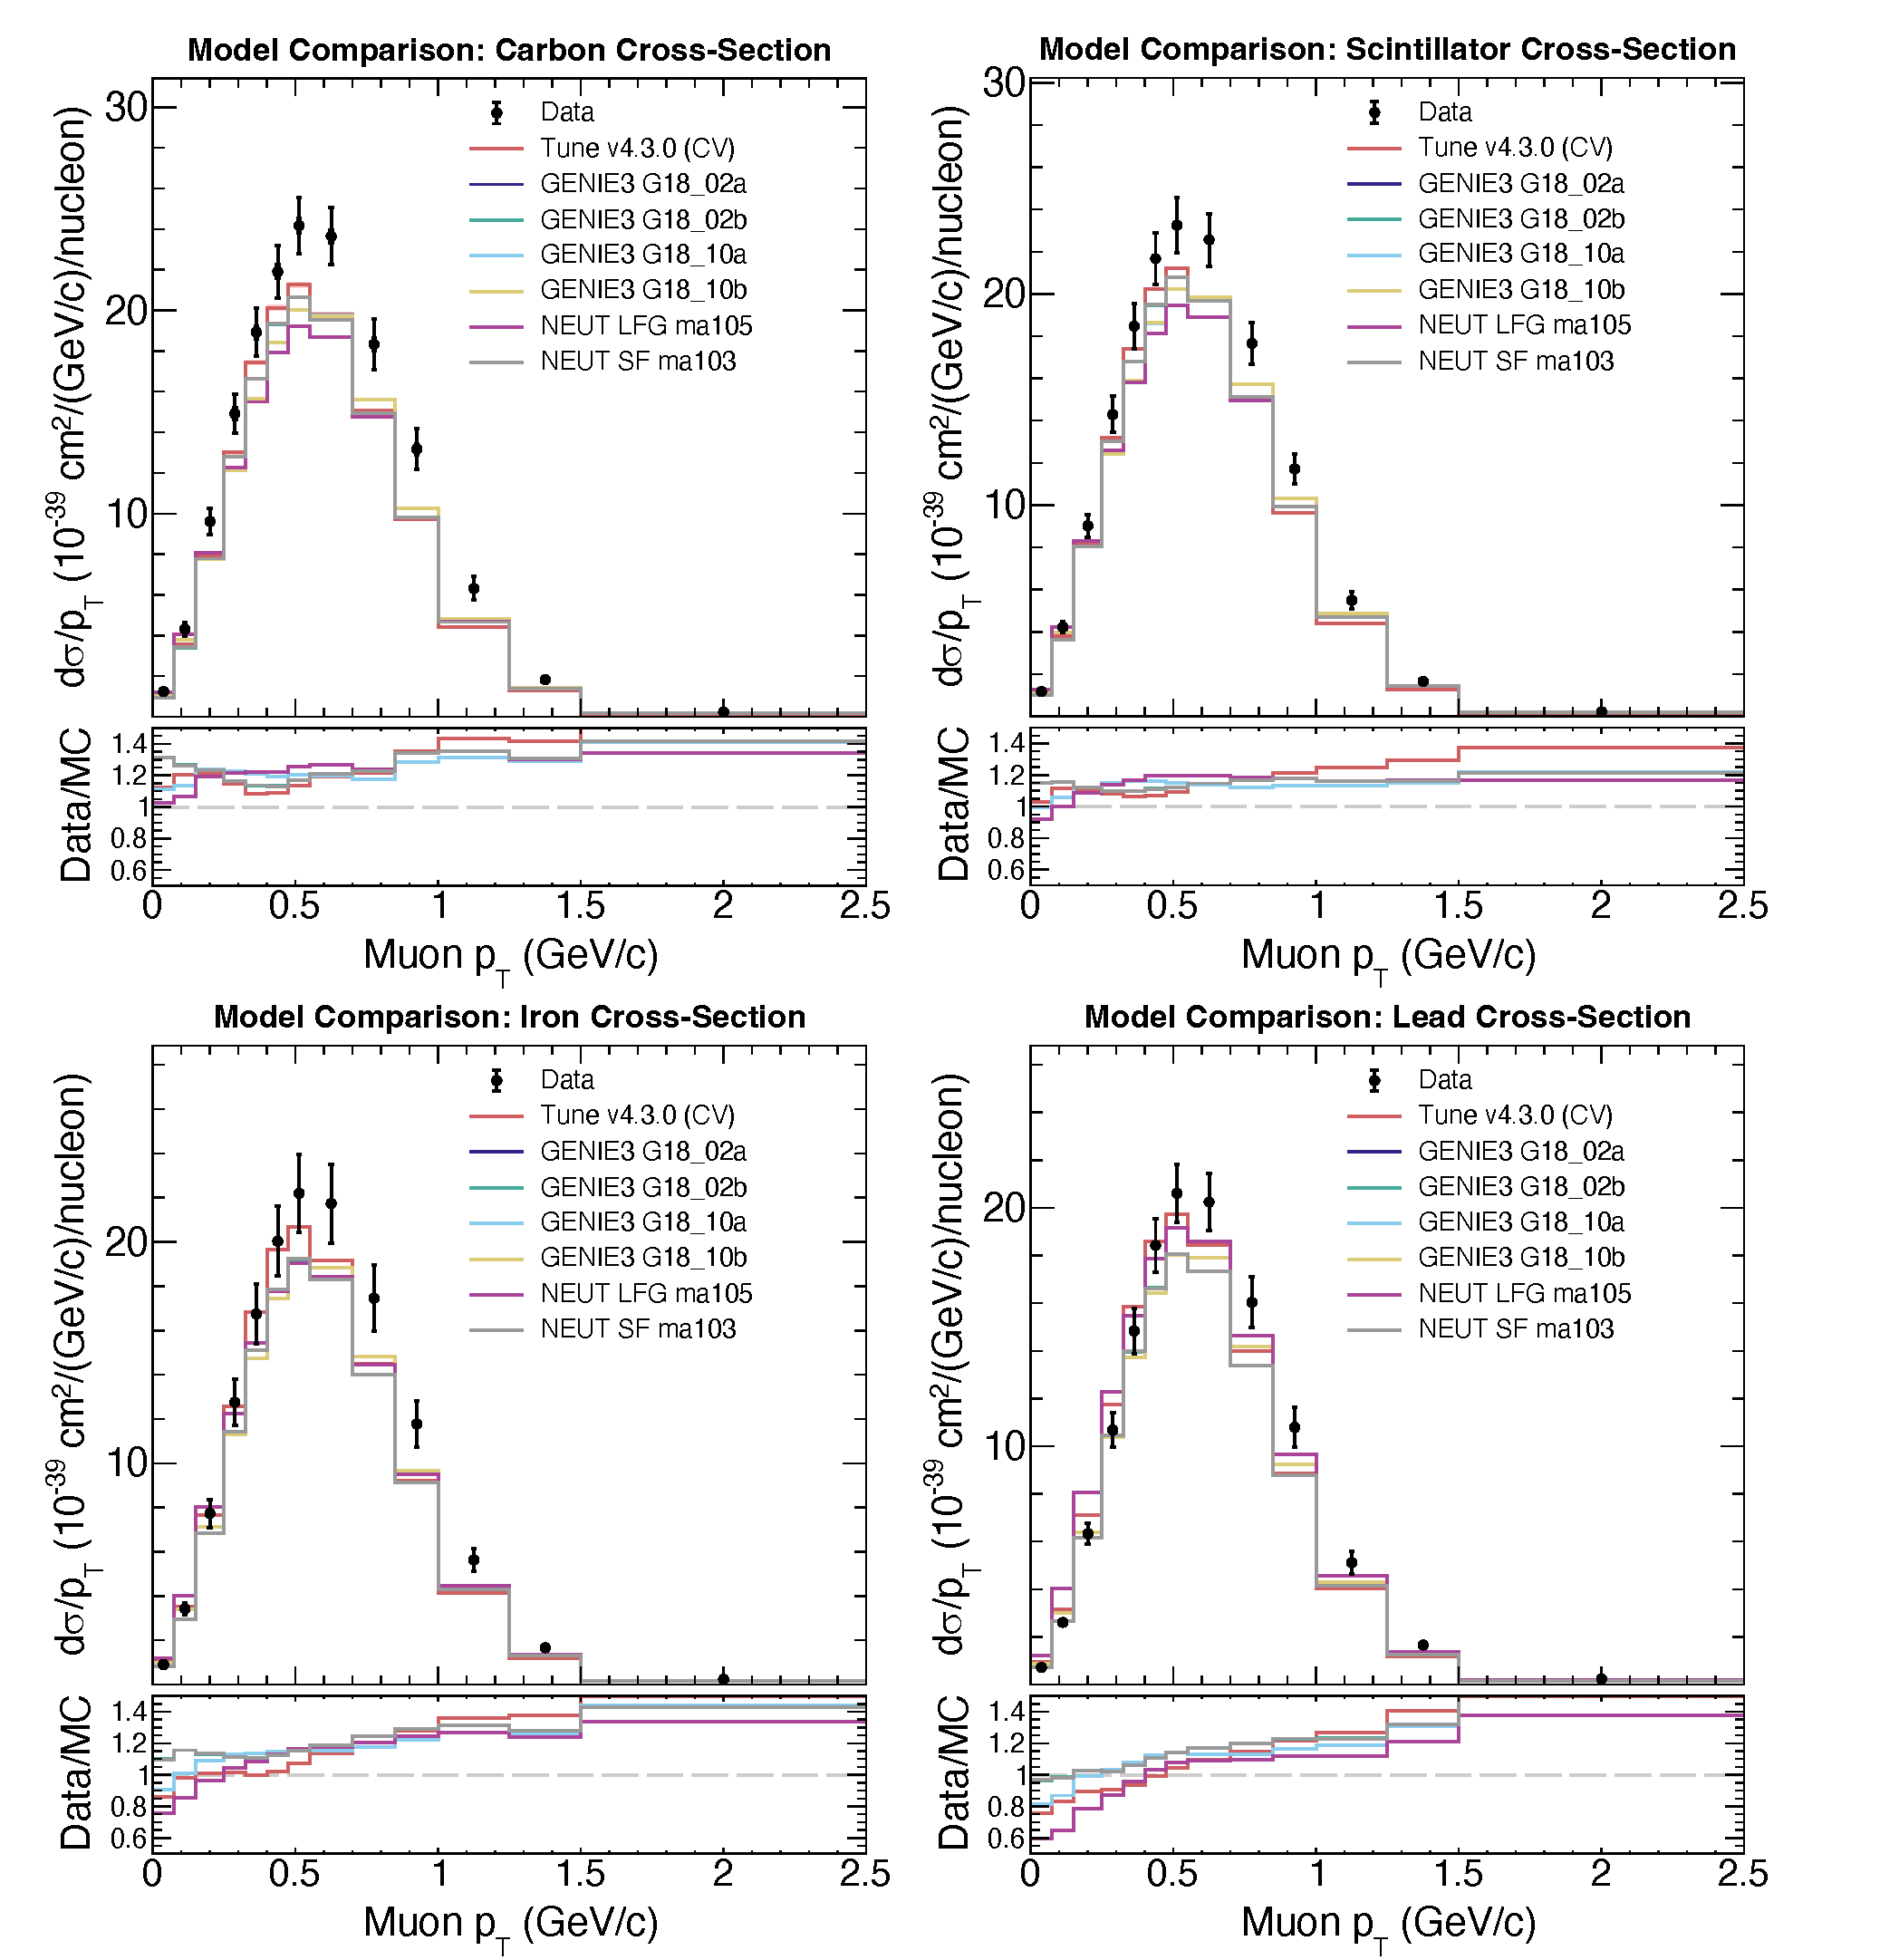
\includegraphics[width=1.\textwidth]{09results/figures/xsec_pT_modelComparison.pdf}}%
    \caption{Measured carbon, scintillator, iron, and lead (from left to right, top to bottom) cross-section as a function of antimuon $p_{\text{T}}$ compared to various antineutrino generator predictions. The inner error bar on the data indicates the statistical error while the outer error bar corresponds to the total, i.e. statistical + systematic, error. The statistical errors on the various model predictions are not shown for clarity (but they are also negligible). The bottom panel indicates the agreement between the data and various models through their respective data-to-model prediction ratios.}
    \label{fig:xsec_pT_modelComparison}
\end{figure}

\begin{figure}[t!] 
    \centering
    {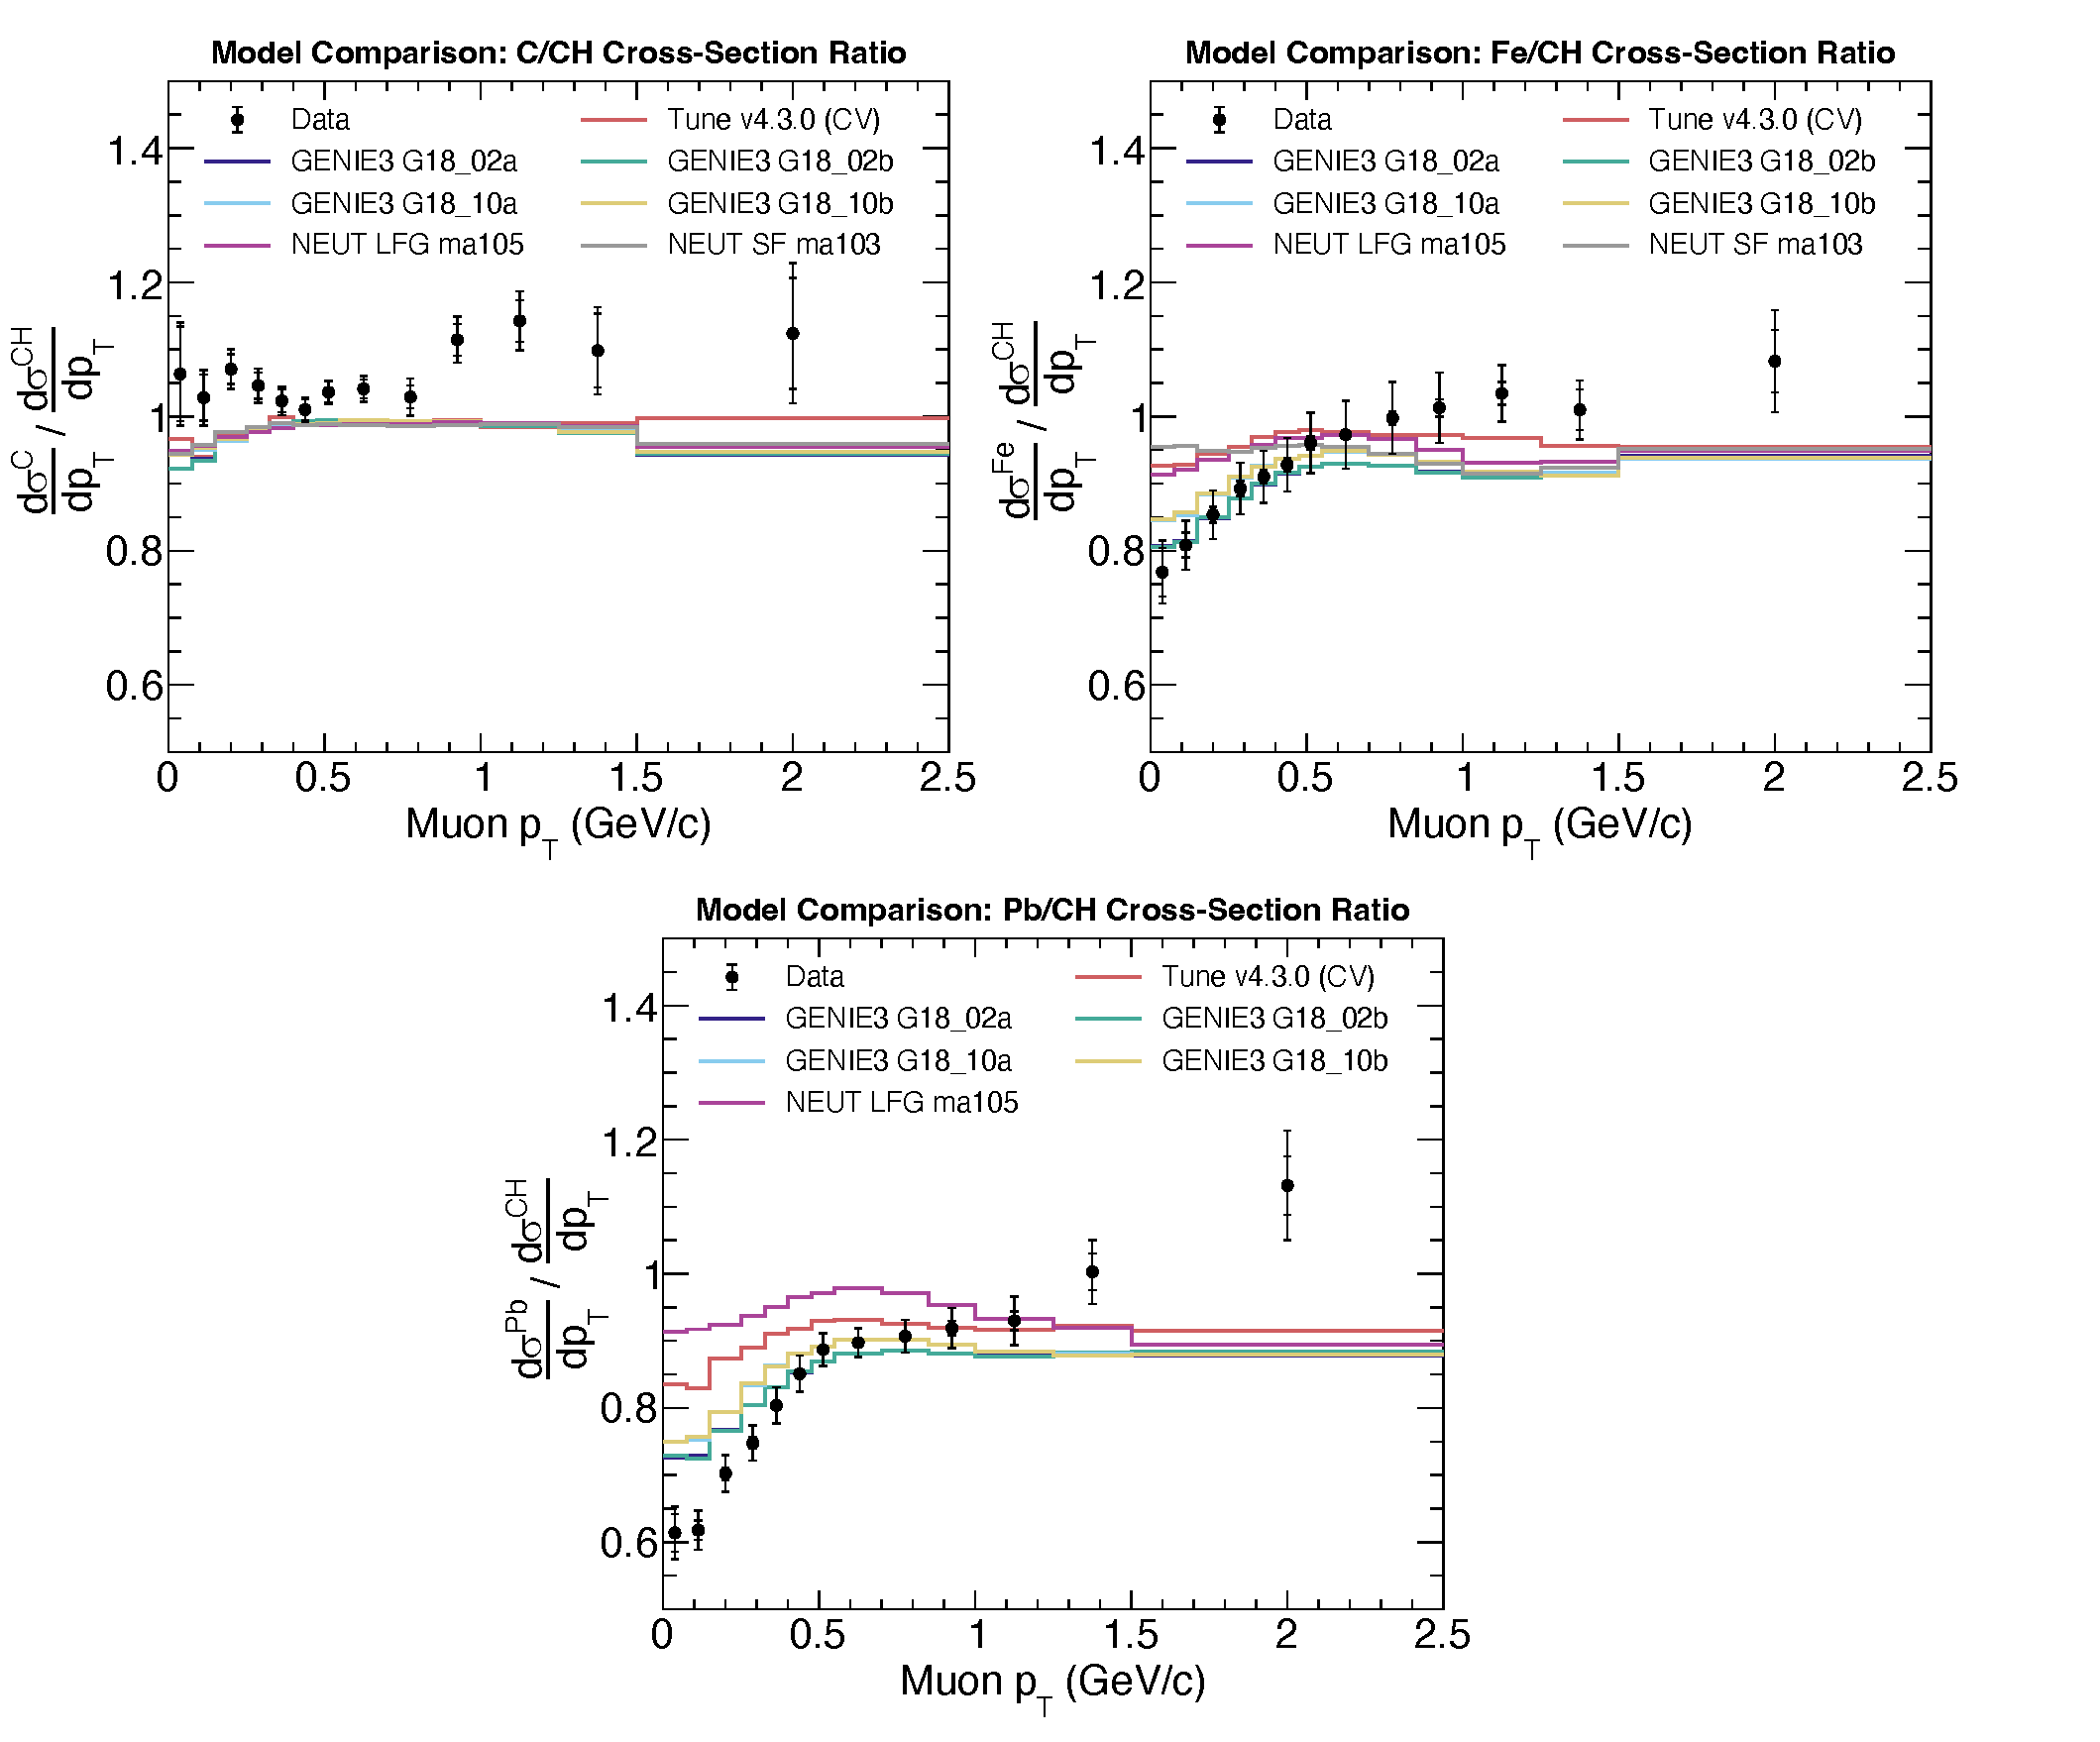
\includegraphics[width=1.\textwidth]{09results/figures/ratios_pT_modelComparison.pdf}}%
    \caption{Measured carbon-to-scintillator (top left), iron-to-scintillator (top right), and lead-to-scintillator (bottom) cross-section ratios in antimuon $p_{\text{T}}$ compared to various antineutrino generator predictions. The data is displayed with both the statistical (inner error bars) and the total (outer error bars) uncertainty. Note that the suppression predicted by the GENIE 3 models at low $p_{\text{T}}$ mostly follows the shape of the data.}
    \label{fig:ratio_pT_modelComparison}
\end{figure}


The $p_{\text{T}}$ cross-section data generally indicates a preference for the new version of GENIE 3, with a slight inclination towards G18\_02a/b. G18\_10a/b, on the other hand, tends to provide a slightly better prediction for the carbon data based on the calculated~$\chi^2$. The improvements over the underlying simulation are likely to stem mainly from better modelling of the low $p_{\text{T}}$ regions using updated axial and vector mass form factors. The NEUT model using the spectral function nuclear ground state performs similarly well for carbon, scintillator, and iron. Overall, the models tend to underpredict the data, except in the low $p_{\text{T}}$ region for heavier nuclei where the models overpredict. All models fail to reproduce the high $p_{T}$ behaviour.
% LFG versus RFG initial-state nucleon models is small because affects mostly CCQE in GENIE and not 2p2h or RES (and nos IDS)

\begin{table}[t!]
    \centering
    \begin{adjustbox}{width=1.01\textwidth,center=\textwidth}
    \begin{tabular}{c c c c c c c c}
    \hline \\ [-1.5 ex]
    \multirow[c]{2}{*}{Cross-section} & \multicolumn{7}{c}{Model $\chi^2$/ndf for $p_{\text{T}}$ (ndf = 13) } \\ [0.8ex]
    & CV & G18\_02a & G18\_02b & G18\_10a & G18\_10b & LFG\_ ma105 & SF\_ma103\\ [0.5ex] % inserts table %heading
    \hline
    \hline \\[-1.9ex]
    Carbon & 2.64 & 2.15 & 2.15 & 1.67 & 1.67 & 2.24 & 2.15 \\
    %\hline
    Scintillator & 10.35 & 4.37 & 4.47 & 12.77 & 12.22 & 40.75 & 4.37\\
    %\hline
    Iron & 3.04 & 1.63 & 1.67 & 3.12 & 3.13 & 9.60 &1.63 \\
    %\hline
    Lead & 6.22 & 3.20 & 3.11 & 9.07 & 9.24 & 39.59 & 3.20 \\

    \hline
    \end{tabular}
    \end{adjustbox}

    \caption{Fully correlated $\chi^2$/ndf calculated according to Equation~\ref{eq:fullyCorrelatedChi2} to assess the agreement between the measured data and the various models for carbon, scintillator, iron, and lead cross-section in antimuon $p_{\text{T}}$. Note that the relatively large $\chi^2$/ndf for the scintillator is attributed to the large statistics of the sample. The first numerical column indicates the agreement with the underlying simulation prediction.}
    \label{table:xsec_modelComparison_pT}
\end{table}


\begin{table}[t!]
    \vspace{20pt}
    \centering
    \begin{adjustbox}{width=1.01\textwidth,center=\textwidth}
    \begin{tabular}{c c c c c c c c}
    \hline \\ [-1.5 ex]
    \multirow[c]{2}{*}{Cross-section ratio} & \multicolumn{7}{c}{Model $\chi^2$/ndf for $p_{\text{T}}$ (ndf = 13) } \\ [0.8ex]
     & CV & G18\_02a & G18\_02b & G18\_10a & G18\_10b & LFG\_ ma105 & SF\_ma103\\ [0.5ex] % inserts table %heading
    \hline
    \hline \\[-1.9ex]
    C/CH & 4.93 & 5.72 & 5.75 & 5.80 & 5.74 & 5.90 & 5.60 \\
    %\hline
    Fe/CH & 2.35 & 1.63 & 1.68 & 1.71 & 1.73 & 3.00 & 3.23 \\
    %\hline
    Pb/CH & 12.06 & 5.06 & 4.80 & 6.11 & 6.41 & 28.79 & 29.40 \\
    \hline
    \end{tabular}    
    \end{adjustbox}
    \caption{Fully correlated $\chi^2$/ndf calculated according to Equation~\ref{eq:fullyCorrelatedChi2} to assess the agreement between the measured data and the various models in the cross-section ratios to scintillator for carbon, iron, and lead in antimuon $p_{\text{T}}$. The first numerical column indicates the agreement with the underlying simulation prediction.}
    \label{table:xsecRatio_modelComparison_pT}
\end{table}


% ratio
The comparisons of cross-section ratios in $p_{\text{T}}$ demonstrate the improved $A$-dependent features of GENIE 3 in the low $p_{\text{T}}$ region. Specifically, the shape of the measured iron-to-scintillator ratio is well-captured by G18\_02a/b. However, the lead-to-scintillator cross-section ratio suggests that additional suppression strength in G18\_02a/b may be necessary. The Pb/CH also indicates a slight preference for the full intranuclear cascade rather than the effective FSI model (which is very slightly preferred by iron).
% hA preferred by carbon and iron. hN preferred by lead, strong FSI

\begin{figure}[t!] 
    \vspace{30pt}
    \centering
    {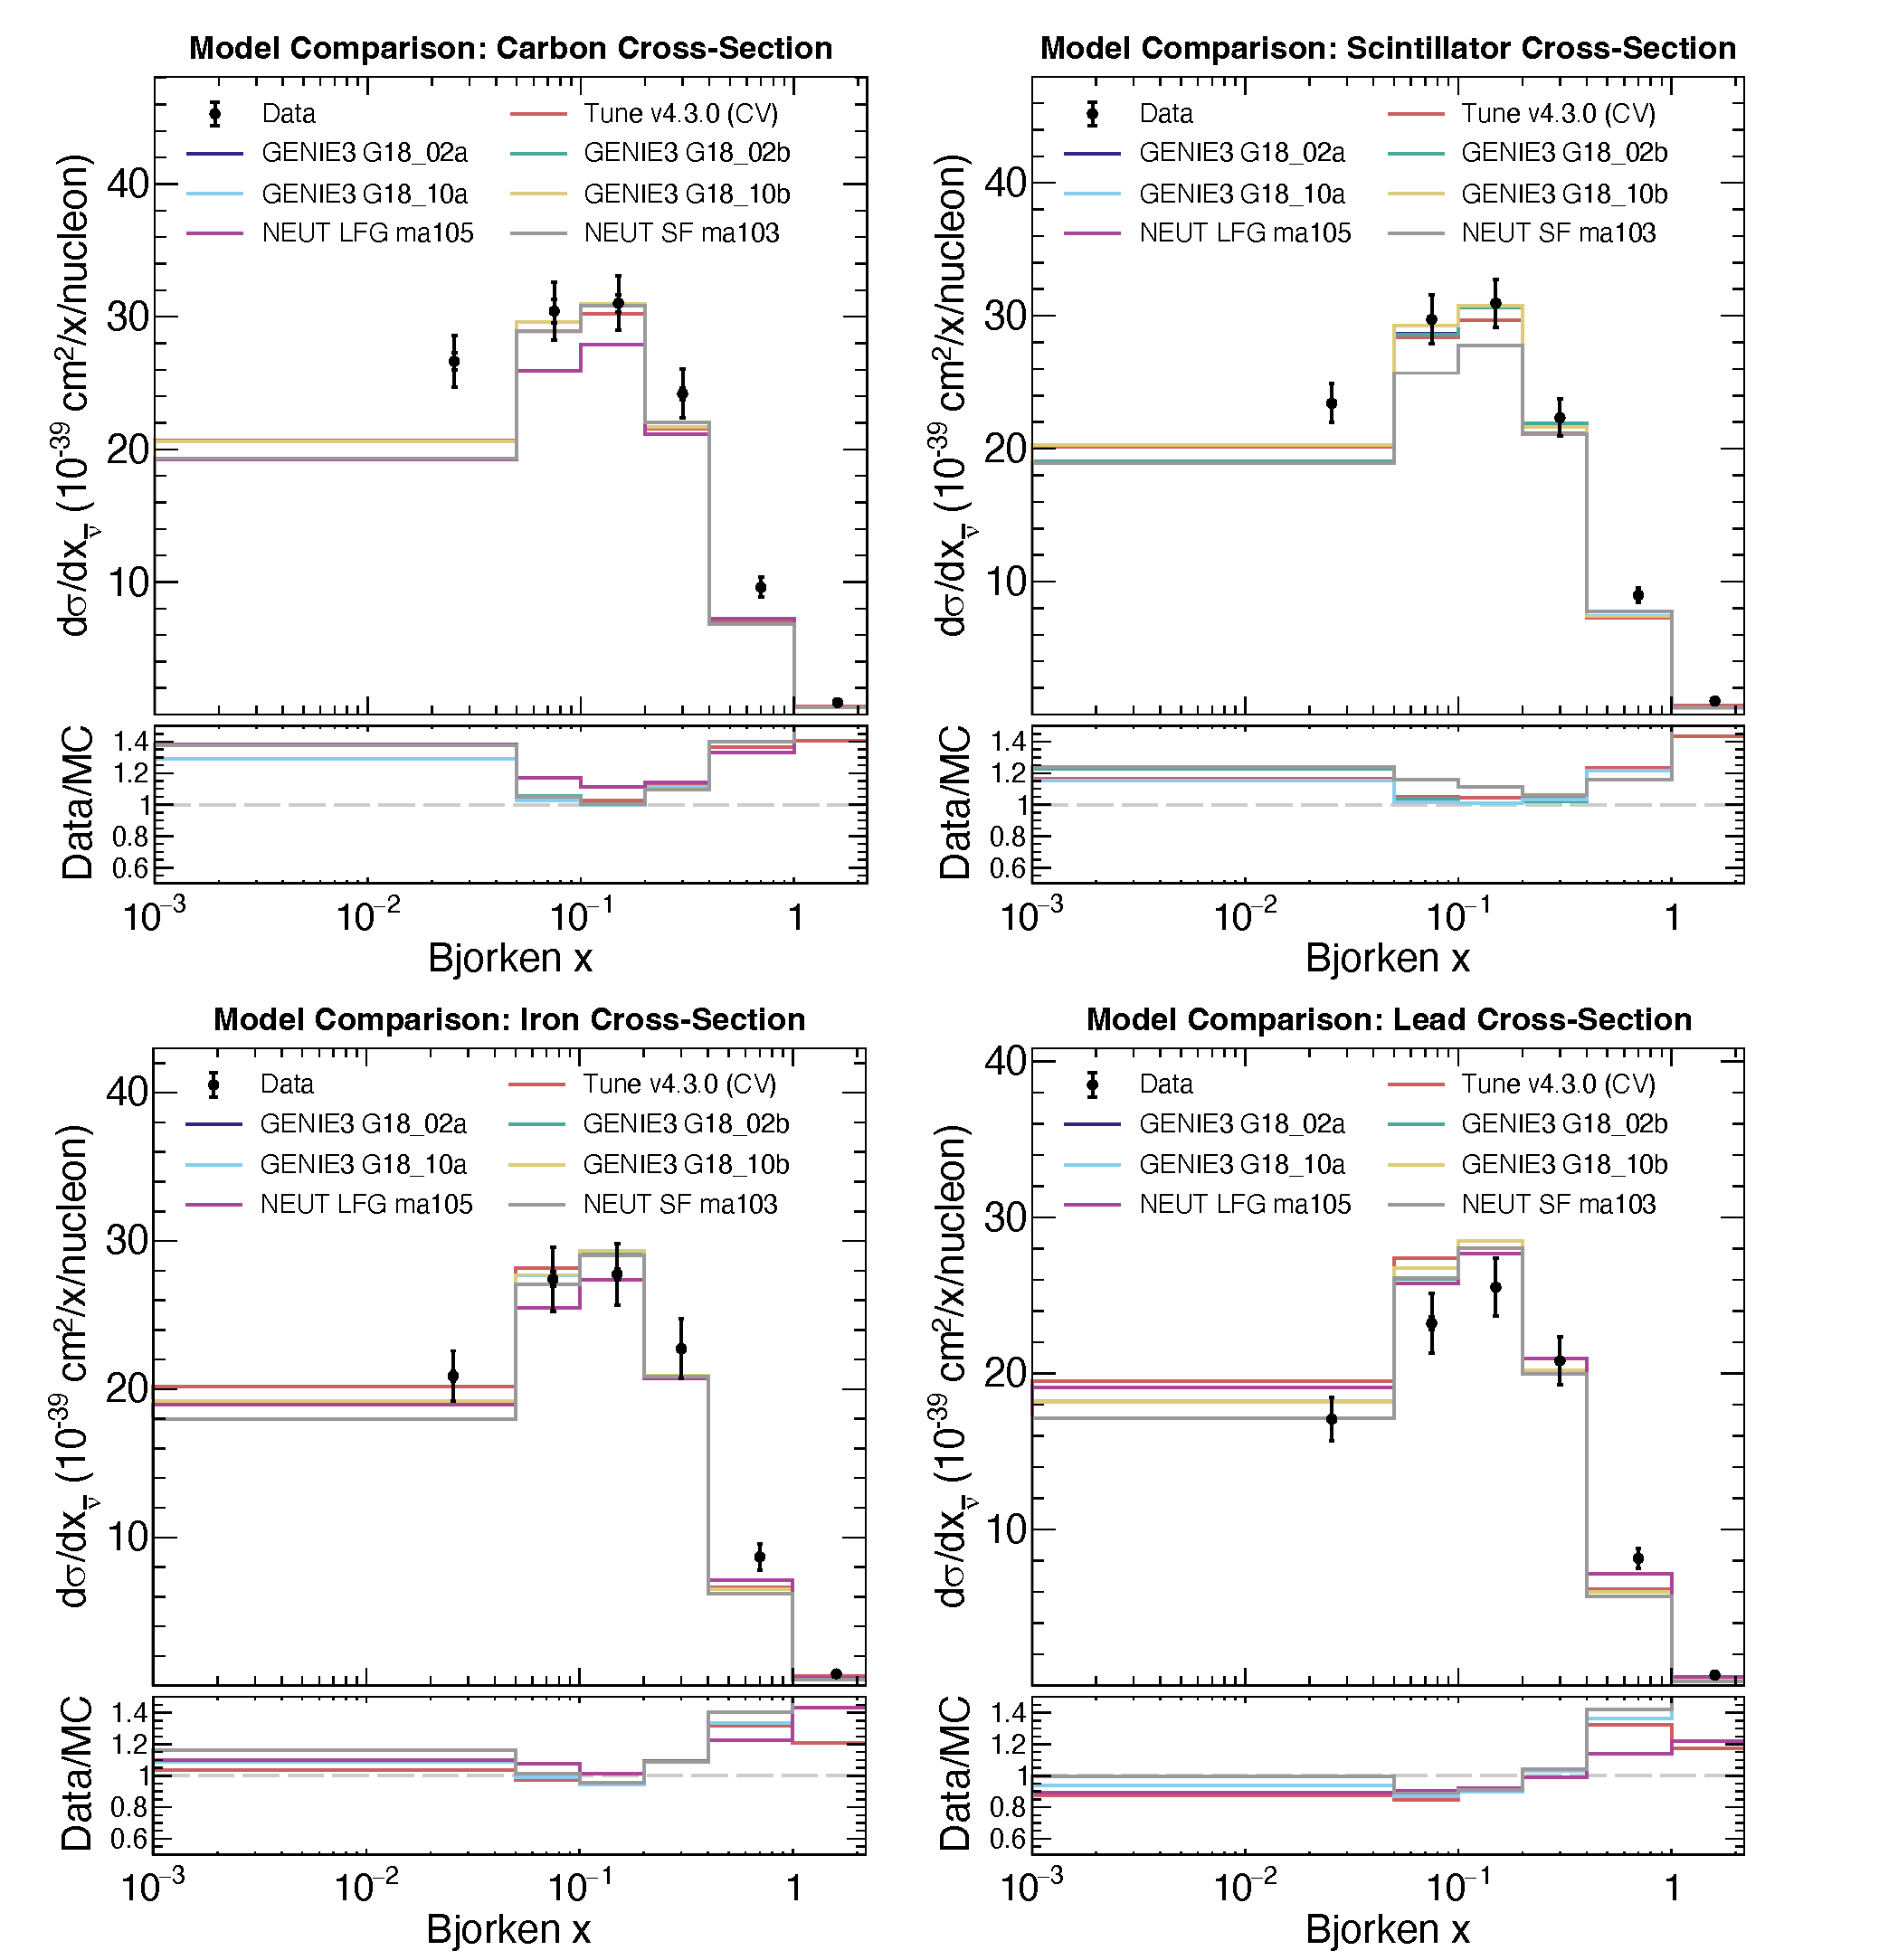
\includegraphics[width=1.\textwidth]{09results/figures/xsec_x_modelComparison.pdf}}%
    \caption{Measured carbon, scintillator, iron, and lead (from left to right, top to bottom) cross-section as a function of Bjorken $x$ compared to various antineutrino generator predictions. The inner error bar on the data indicates the statistical error while the outer error bar corresponds to the total, i.e. statistical + systematic, error. The statistical errors on the various model predictions are not shown for clarity (but they are also negligible). The bottom panel indicates the agreement between the data and various models through their respective data-to-model prediction ratios.}
    \label{fig:xsec_x_modelComparison}
\end{figure}

% bjorken x
The Bjorken $x$ cross-section results across the various nuclei prefer both NEUT implementations over GENIE 3. Specifically, the local Fermi gas model appears to perform quite well. This preference could potentially be attributed to differences in the treatment of the resonant pion production to deep inelastic scattering transition region compared to GENIE, or the distinct intranuclear cascade. However, further investigation would be required for a more detailed understanding.

% bjorken x ratio
In contrast, many of the differences between the data and the models cancel out in the Bjorken $x$ cross-section ratios to the scintillator. Consequently, GENIE 3 shows its strength in modeling the $A$-dependence of the overall cross-section again. Both G18\_02a/b and G18\_10a/b predict the suppression in the low-$x$ region relatively well, with the Pb/CH ratio requiring additional strength, similar to the $p_{\text{T}}$ ratios.

\begin{figure}[t!] 
    \centering
    {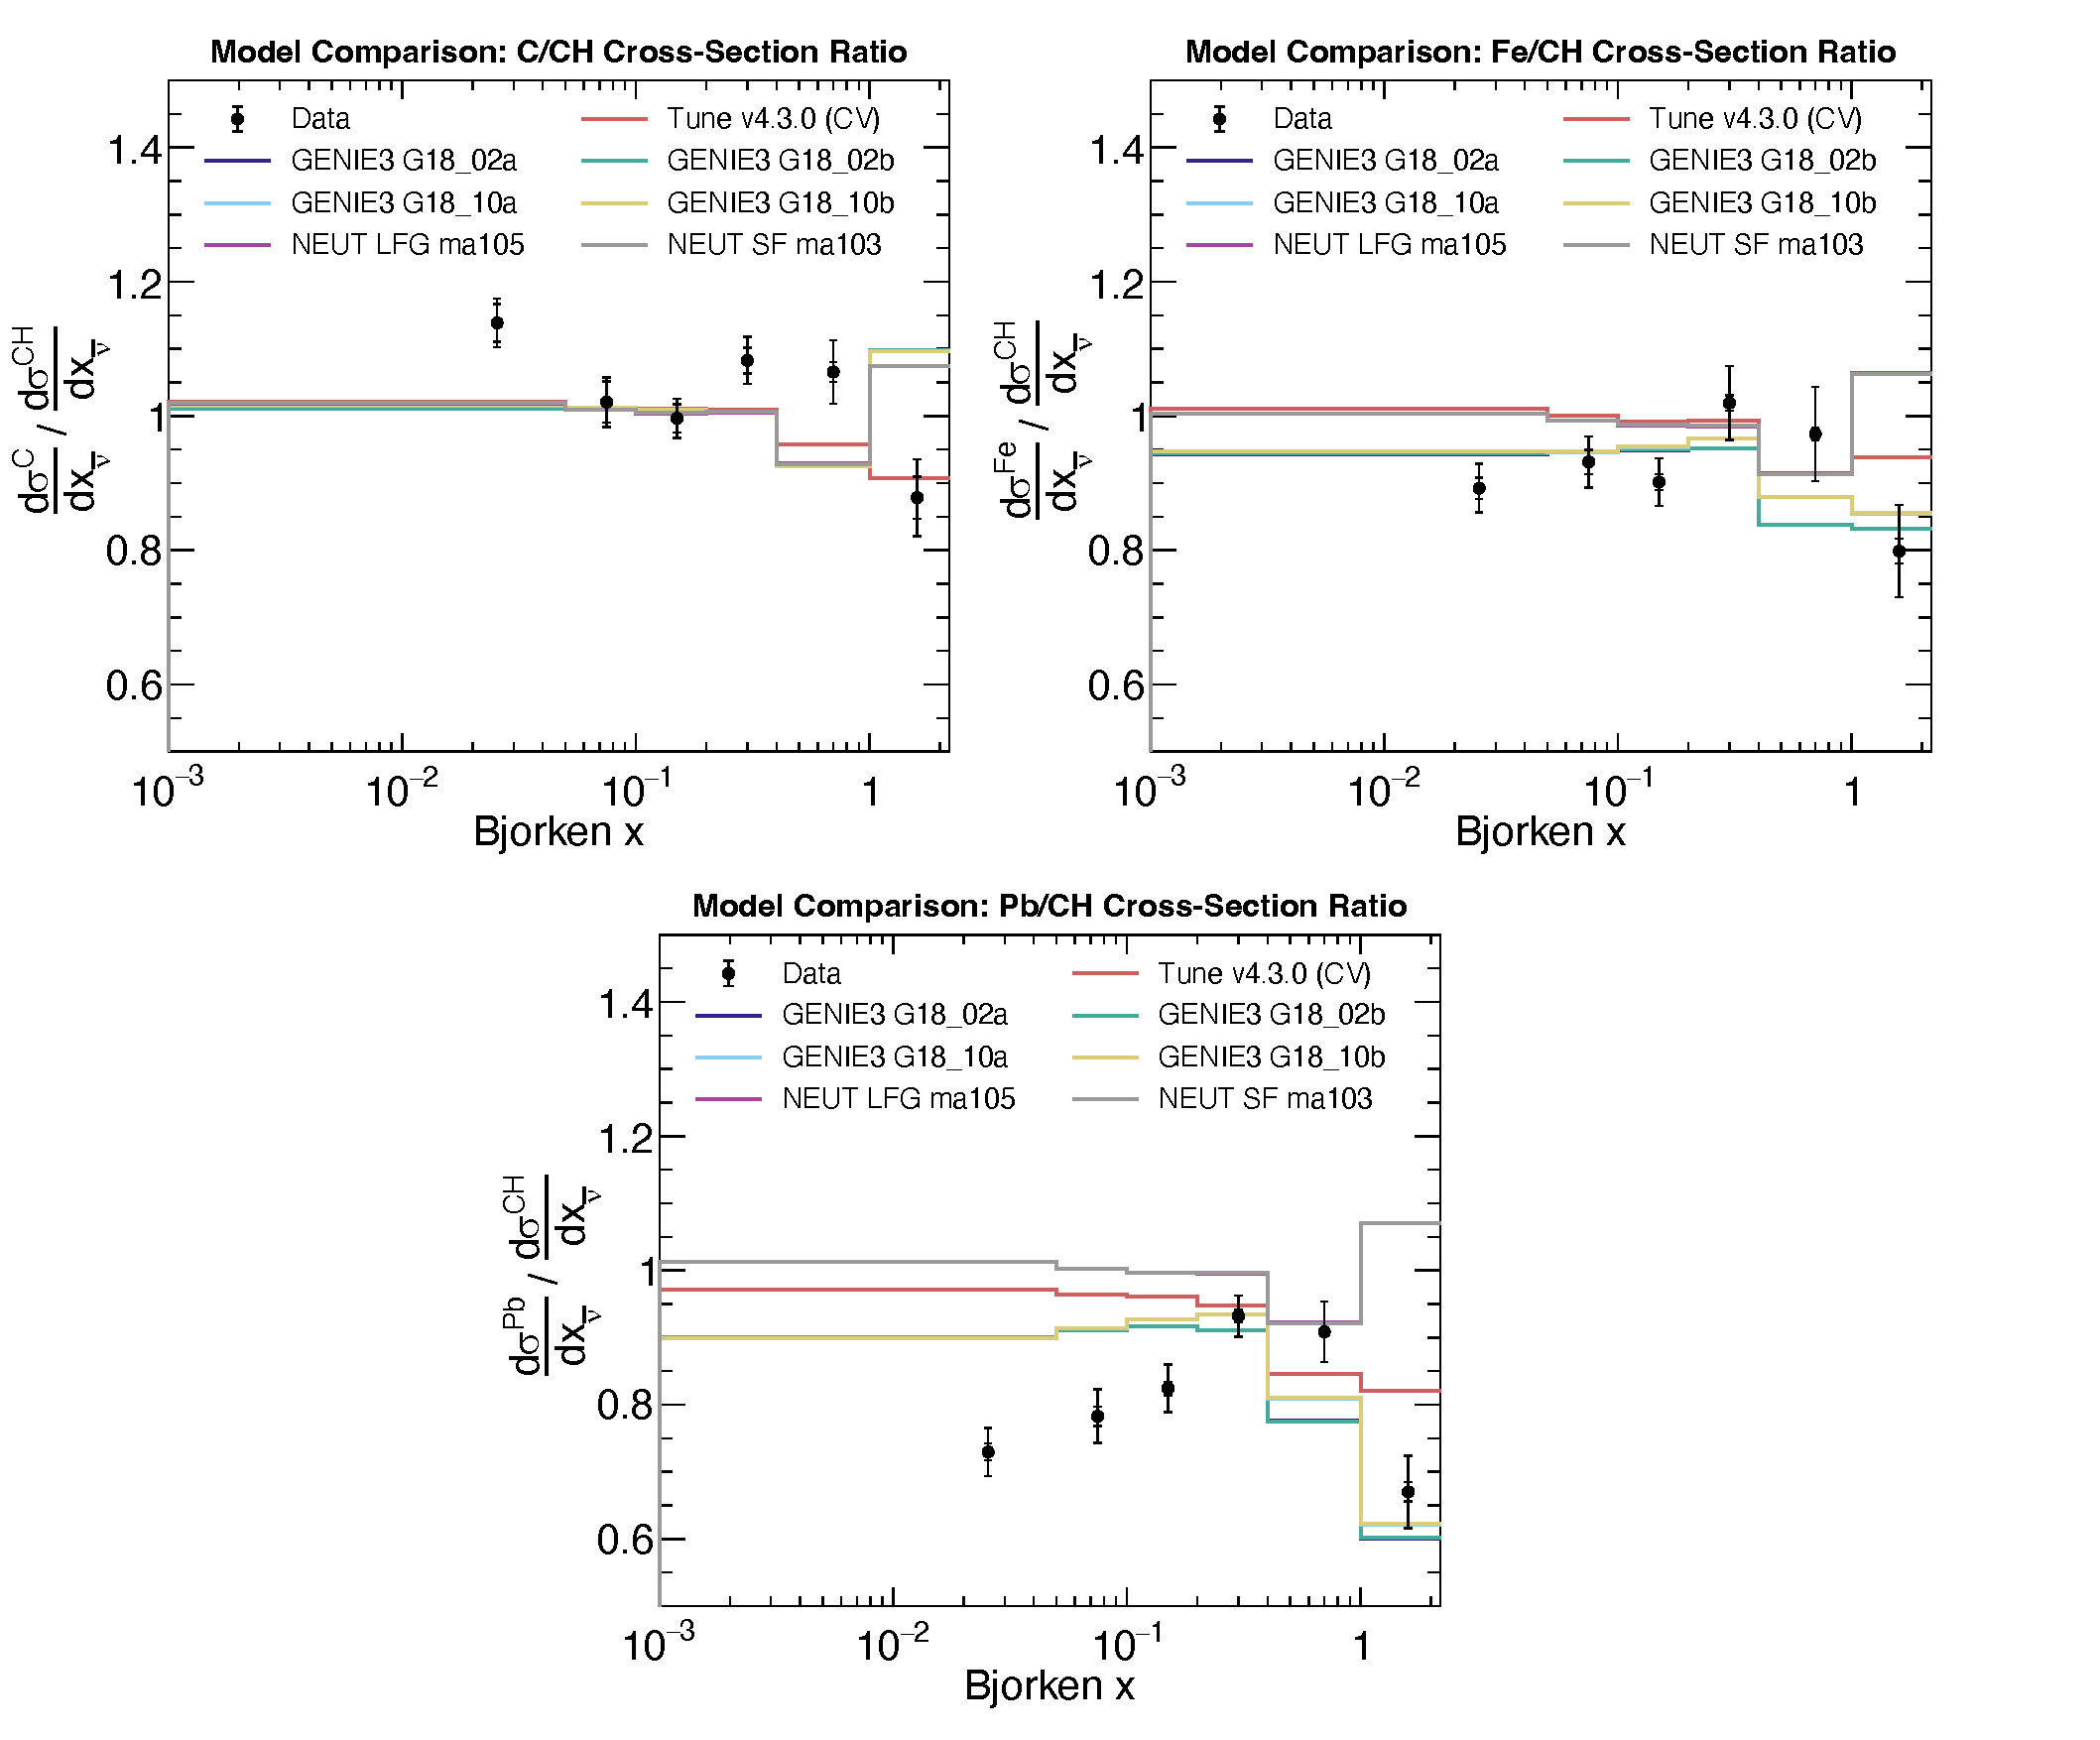
\includegraphics[width=1.\textwidth]{09results/figures/ratios_x_modelComparison.pdf}}%
    \caption{Measured carbon-to-scintillator (top left), iron-to-scintillator (top right), and lead-to-scintillator (bottom) cross-section ratios in Bjorken $x$ are compared to various antineutrino generator predictions. The data is displayed with both the statistical (inner error bars) and the total (outer error bars) uncertainty. The suppression predicted by the GENIE 3 models at low Bjorken $x$ attempts to follow the shape of the data.}
    \label{fig:ratio_x_modelComparison}
\end{figure}

\begin{table}[b!]
    \vspace{-18pt}
    \centering
    \begin{adjustbox}{width=1.01\textwidth,center=\textwidth}
    \begin{tabular}{c  c c c c c c c}
    \hline \\ [-1.5 ex]
    \multirow[c]{2}{*}{Cross-section} & \multicolumn{7}{c}{Model $\chi^2$/ndf for Bjorken $x$ cross-section (ndf = 6) } \\ [0.8ex]
    & CV & G18\_02a & G18\_02b & G18\_10a & G18\_10b & LFG\_ ma105 & SF\_ma103\\ [0.5ex] % inserts table %heading
    \hline
    \hline \\[-1.9ex]
    Carbon & 5.34 & 8.44 & 8.47 & 7.02 & 7.07 & 4.47 & 8.44\\
    %\hline
    Iron & 3.50 & 7.64 & 7.64 & 5.98 & 6.10 & 2.07 & 7.64 \\
    %\hline
    Lead & 4.46 & 5.94 & 5.92 & 5.19 & 5.23 & 1.27 & 5.94 \\
    %\hline
    Scintillator & 17.22 & 44.61 & 44.30 & 29.79 & 30.12 & 10.49 & 10.49 \\
    \hline
    \end{tabular}
    \end{adjustbox}
    \caption{Fully correlated $\chi^2$/ndf calculated according to Equation~\ref{eq:fullyCorrelatedChi2} to evaluate the agreement between the measured data and the various models for carbon, scintillator, iron, and lead cross-section in Bjorken $x$. Note that the relatively large $\chi^2$/ndf for the scintillator is attributed to the large statistics of the sample. The first numerical column indicates the agreement with the underlying simulation prediction.}
    \label{table:xsec_modelComparison_x}
\end{table}
\clearpage
\begin{table}[t!]
    \centering
    \begin{adjustbox}{width=1.01\textwidth,center=\textwidth}
    \begin{tabular}{c c c c c c c c}
    \hline \\ [-1.5 ex]
    \multirow[c]{2}{*}{Cross-section ratio} & \multicolumn{7}{c}{Model $\chi^2$/ndf for Bjorken $x$ (ndf = 6) } \\ [0.8ex]
     & CV & G18\_02a & G18\_02b & G18\_10a & G18\_10b & LFG\_ ma105 & SF\_ma103\\ [0.5ex] % inserts table %heading
    \hline
    \hline \\[-1.9ex]
    C/CH & 5.91 & 5.80 & 5.85 & 5.73 & 5.71 & 5.60 & 5.53 \\
    %\hline
    Fe/CH & 6.28 & 3.39 & 3.47 & 3.01 & 3.08 & 9.95 & 9.91 \\
    %\hline
    Pb/CH & 12.69 & 11.14 & 11.13 & 7.74 & 7.69 & 20.19 & 20.24 \\
    \hline
    \end{tabular}    
    \end{adjustbox}
    \caption{Fully correlated $\chi^2$/ndf calculated according to Equation~\ref{eq:fullyCorrelatedChi2} to assess the agreement between the measured data and the various models in the cross-section ratios to scintillator for carbon, iron, and lead in Bjorken $x$. The first numerical column indicates the agreement with the underlying simulation prediction.}
    \label{table:xsecRatio_modelComparison_x}
\end{table}

% tunes in the appendix
Finally, various MINERvA results are also reported with different MINERvA tunes applied to the base GENIE 2.12.6, i.e. tunes different from the underlying v4.3.0~used in this analysis. To enable further review of the results of this analysis in the context of other MINERvA results, the comparisons of the measured cross-sections and cross-section ratios are included in Appendix~\ref{ch:appendix_tuneComparisons}. 

\section{Extension to two dimensions}
\label{sec:analysis2D}

%\section{Differences compared to 1D}
%\section{2D Cross-section distributions}
%\section{2D Cross-section ratios}



% some other notes
%In summary, these data on single pion production on a wide variety of nuclei provide a new way to test nuclear models through their nuclear dependence. We observe a large modification to the predicted Q2 distribution of single pi+ events that it can be consistently seen in all nuclei. These results give guidance in how the wealth of data on scintillator targets can be applied to models for oxygen and argon for future neutrino experiments.
    
% Combined with other measurements from MINERvA
% These measurements combined provide key benchmarks for the field’s description of how the nucleus impacts neutrino interactions
    

%It has been experimentally demonstrated that the structure of the nucleon in the nuclear environment is indeed different than the free nucleon structure. Understanding this modified structure has played an important part in the experimental and theoretical exploration of nucleon structure by neutrinos and is one of the important goals of the on-going MINERvA experiment at Fermilab.
    
    

\clearpage
\thispagestyle{empty}
\hfill
\clearpage
\chapter{Conclusions and outlook}

\label{ch:conclusions}

% conclusions

Something reference \cite{NeutrinosBook}





- say what is the percentage uncertainty on the cross-section
\clearpage
\thispagestyle{empty}
\hfill
\clearpage

% Formatting of Bibligraphy
\addcontentsline{toc}{chapter}{Bibliography}
%\bibliographystyle{alpha}
\bibliographystyle{unsrturl2authabbrvpp}
\bibliography{bibliography/bibliography.bib}

%\chapter*{Glossary of terms, abbreviations, and acronyms}
\markboth{Glossary of terms, abbreviations, and acronyms}{Glossary of terms, abbreviations, and acronyms}

\begin{spacing}{1.5}
\begin{longtable}[l]{p{0.28\textwidth} p{0.68\textwidth}}
    \textbf{2p2h} & Two-particle-two-hole interaction resulting in two nucleons in the final state \\
        \textbf{$A$} & Mass number of a given nucleus referring to the number of nucleons (protons + neutrons) \\
        \textbf{$A$-dependence} & Nuclear dependence \\
        \textbf{ADC} & \textbf{A}nalog-to-\textbf{D}igital \textbf{C}onverter of the signal \\
        \textbf{AGKY} & \textbf{A}ndreopoulous-\textbf{G}allagher-\textbf{K}ehayias-\textbf{Y}ang model describing the hadronisation process in GENIE \\
        \textbf{Baffle} & Graphite-aluminum tube designed to partially degrade mis-steered beams to protect other components of the beamline \\
        \textbf{Calorimetric spline} & Piecewise calorimetric correction applied to reconstructed recoil energy to account for deposition in passive material, limited containment, and invisible energy deposits in the detector from particles such as neutrons    \\
        \textbf{CC} & \textbf{C}harged-\textbf{C}urrent interaction wherein (anti)neutrino exchanges a $W^{\pm}$ boson, converting into its coupled charged lepton \\
        \textbf{CP} & \textbf{C}harge-\textbf{P}arity symmetry  \\
        \textbf{DAQ} & \textbf{D}ata \textbf{A}c\textbf{Q}uisition, the system that receives raw data from the detector, digitises them, and stores them on disk \\
        \textbf{`Daisy petal'} & One of the 12 transverse bins in which the hexagonal cross-section of the scintillator tracker is divided for the flux and differential cross-section calculation \\
        \textbf{`Daisy reweight'} & Linear combination of the scintillator distributions extracted in 12 `daisy petals' to match the flux of the scintillator tracker to that of a given nuclear target in cross-section ratios  \\
        \textbf{DCNN} & \textbf{D}eep \textbf{C}onvolutional \textbf{N}eural \textbf{N}etwork used in this work to reconstruct the interaction vertex  \\
        \textbf{DIS} & \textbf{D}eep \textbf{I}nelastic \textbf{S}cattering interaction channel in which a high-energetic (anti)neutrino interacts with the constituents of nucleons, producing a hadronic shower  \\
        \textbf{Downstream} & Relative position with respect to the (anti)neutrino beam referring to a position \textit{in} the direction of the beam   \\
        \textbf{DUNE} & \textbf{D}eep \textbf{U}nderground \textbf{N}eutrino \textbf{E}xperiment, predominantly argon-based future neutrino oscillation experiment  \\
        \textbf{ECAL} & \textbf{E}lectromagnetic \textbf{CAL}orimeter designed to contain electromagnetic showers  \\
        \textbf{EMC effect} & \textbf{E}uropean \textbf{M}uon \textbf{C}ollaboration effect; one of the observed nuclear modifications to structure functions describing depletion in the bound nucleon cross-section ratio in the $0.3 \lesssim x \lesssim 0.7$   \\ 
        \textbf{FEB} & \textbf{F}ront-\textbf{E}nd \textbf{B}oard; electronics board attached on top of a PMT that digitises the output signal from the PMT \\
        \textbf{Fermi motion} & Isotropic initial state movement of nucleons inside the nuclear environment \\
        \textbf{FHC} & \textbf{F}orward \textbf{H}orn \textbf{C}urrent configuration of the magnetic horns in the beamline, resulting in neutrino-dominated beam  \\
        \textbf{FSI} & \textbf{F}inal \textbf{S}tate \textbf{I}nteractions that particles produced by (anti)neutrino interactions with nucleons inside the nucleus can undergo prior to exiting the nucleus \\
        \textbf{G4NuMI} & \textbf{G}EANT\textbf{4} package for simulation of the \textbf{NuMI} beamline  \\
        \textbf{Gate} & MINERvA's data-taking period of 16~$\mu$s   \\
        \textbf{GENIE} & \textbf{G}enerates \textbf{E}vents for \textbf{N}eutrino \textbf{I}nteraction \textbf{E}xperiments; (anti)neutrino-nucleus interaction simulation, also known as event generator, used to model (anti)neutrino interactions and make predictions  \\
        \textbf{GENIEXSecExtract} & MINERvA's cross-section validation tool, which is external to the analysis framework \\
        \textbf{GEANT4} & \textbf{GE}ometry \textbf{AN}d \textbf{T}racking software used for detector geometry and particle propagation through the detector modelling \\
        \textbf{HCAL} & \textbf{H}adronic \textbf{CAL}orimeter designed to contain hadronic showers   \\
        \textbf{Horn} & Parabolic focusing and charge-sign selecting magnet used in the (anti)neutrino beamline setup \\
        \textbf{ID} & \textbf{I}nner \textbf{D}etector  \\
        \textbf{Inclusive} & Considering all final states, i.e.~all (anti)neutrino interaction modes \\
        \textbf{INTRANUKE} & Intranuclear cascade simulation used in GENIE to model FSI  \\
        \textbf{KNO} & \textbf{K}oba-\textbf{N}ielsen-\textbf{O}lesen phenomenological model used in GENIE's AGKY hadronisation model to describe the hadronisation process for events with lower invariant mass \\
        \textbf{LE} & \textbf{L}ow \textbf{E}nergy regime of the NuMI beam and corresponding MINERvA data-taking period with (anti)neutrino flux with(anti)neutrino energy peak of $\sim$3~GeV  \\
        \textbf{LFG} & \textbf{L}ocal \textbf{F}ermi \textbf{G}as model for the initial state of the nucleons inside the nucleus taking into account the local density at the interaction vertex \\
        \textbf{MAT} & \textbf{M}INERvA \textbf{A}nalysis \textbf{T}oolkit used in MINERvA analyses mainly handling the propagation of systematic uncertainties \\
        \textbf{ME} & \textbf{M}edium \textbf{E}nergy regime of the NuMI beam and corresponding MINERvA data-taking period with (anti)neutrino flux with(anti)neutrino energy peak of $\sim$6~GeV\\
        \textbf{MEC} & \textbf{M}eson \textbf{E}xchange \textbf{C}urrent correlating nucleons inside the nuclear environment via an exchange of virtual mesons, often pions\\
        \textbf{MC} & \textbf{M}onte \textbf{C}arlo simulation refers to the (anti)neutrino interaction simulation  \\
        \textbf{Migration} & Process of smearing of the reconstructed kinematics of an event from its true kinematics due to finite detector resolution and imperfect reconstruction described by migration matrix  \\
        \textbf{MINERvA} & \textbf{M}ain \textbf{I}njector \textbf{N}eutrino \textbf{E}xpe\textbf{R}iment to study \textbf{$\nu$}--\textbf{A} interactions, a dedicated cross-section experiment  \\
        \textbf{MINOS} & \textbf{M}ain \textbf{I}njector \textbf{N}eutrino \textbf{O}scillation \textbf{S}earch, a neutrino oscillation experiment; in the context of this work often refers to its near detector only, which was positioned downstream of the MINERvA detector  \\
        \textbf{ML} & \textbf{M}achine \textbf{L}earning, refers to the technique used to reconstruct the interaction vertex \\
        \textbf{Module} & MINERvA's detector tracking unit which refers to two planes of scintillator strips  \\
        \textbf{MIP} & \textbf{M}inimum \textbf{I}onising \textbf{P}article such as (anti)muon   \\
        \textbf{NC} & \textbf{N}eutral-\textbf{C}urrent interaction wherein (anti)neutrino exchanges a $Z$ boson with no charge transfer and leaves the interaction without changing to its paired charged lepton \\
        \textbf{NEUT} & Another (anti)neutrino event generator predominantly used in Japanese experiments, such as the neutrino oscillation experiment T2K  \\
        \textbf{Nuclear target} & Passive material interlaid between the active scintillator planes in MINERvA consisting of combinations of carbon, iron, and lead in the context of this work (there is also a water and helium target)  \\
        \textbf{NuMI} & \textbf{N}eutrinos ({$\bm{\nu}$}) at the \textbf{Main} \textbf{I}njection; (anti)neutrino beam production setup at Fermilab   \\
        \textbf{OD} & \textbf{O}uter \textbf{D}etector   \\
        \textbf{PDFs} & \textbf{P}arton \textbf{D}istribution \textbf{F}unctions describing the distribution of partons within the nucleus  \\
        \textbf{PMNS matrix} & \textbf{P}ontecorvo-\textbf{M}aki-\textbf{N}akagawa-\textbf{S}akata mixing matrix relating the neutrino mass eigenstates and the neutrino flavour eigenstates, describing neutrino oscillation  \\
        \textbf{PMT} & \textbf{P}hoto\textbf{M}ultiplier \textbf{T}ube with 64 channels converting the collected light into charge \\
        \textbf{Plane} & MINERvA's detector tracking unit made of scintillator strips, with either $X$, $U$, or $V$ orientation of the scintillator strips (parallel to the $y$-axis, 60$^{\circ}$ clockwise and anticlockwise, respectively)   \\
        \textbf{Plastic} & Refers to the hydrocarbon scintillator used to make the active tracker region or the scintillator planes in between the nuclear targets  \\
        \textbf{Playlist} & Lists of MINERvA runs and subruns that correspond to a specific detector configuration during a data-taking period \\
        \textbf{POT} & \textbf{P}rotons \textbf{O}n \textbf{T}arget; a metric used to characterise the integrated luminosity of the (anti)neutrino beam \\
        \textbf{PPFX} & \textbf{P}ackage to \textbf{P}redict the \textbf{F}lu\textbf{X} used to constrain flux predictions by external data and evaluate systematic uncertainties  \\
        \textbf{PYTHIA/JETSET} & Standard tool for generation of high-energy collisions, spanning models for few-body hard processes to complex multihadronic final states used in GENIE's AGKY hadronisation model to describe the hadronisation process for events with higher invariant mass \\
        \textbf{Recoil} & Refers to either the total outgoing hadronic system in an interaction, or more specifically to its energy \\
        \textbf{RES} & \textbf{RES}onant pion production interaction channel in which the (anti)neutrino is energetic enough to excite a nucleon into a baryon resonance which then decays, most often to pions \\
        \textbf{RFG} & \textbf{R}elativistic \textbf{F}ermi \textbf{G}as model for initial state of the nucleons inside the nucleus, treating nucleons as a collection of non-interacting fermions in a constant nuclear potential \\
        \textbf{RHC} & \textbf{R}everse \textbf{H}orn \textbf{C}urrent configuration of the magnetic horns in the beamline, resulting in antineutrino-dominated beam   \\
        \textbf{RPA} & \textbf{R}andom \textbf{P}hase \textbf{A}pproximation accounting for long-range correlations in (anti)neutrino-nucleus scattering, arising from the polarisation of the nuclear medium by the electroweak propagator \\
        \textbf{SF} & \textbf{S}pectral \textbf{F}unction model for the initial state of the nucleons inside the nucleus, taking into account two- and three-body nucleon-nucleon interactions, thereby modifying the available nuclear quantum states \\
        \textbf{Shadowing} & Suppression of the cross-section of bound nucleons due to destructive interference of hadronic fluctuations of the intermediate boson that multiple-scatter off surface nucleons at $x \lesssim 0.1$ compared to a free nucleon  \\
        \textbf{SIS} & \textbf{S}hallow \textbf{I}nelastic \textbf{S}cattering referring to the transition region between RES and DIS interaction channels with non-resonant pion production and multi-pion final states, defined by \mbox{$(m_N + m_{\pi}) < W < 2$ GeV/$c^2$} and $Q^2$ around 1 (GeV/$c$)$^2$ \\
        \textbf{SM} & \textbf{S}tandard \textbf{M}odel of particle physics, categorising all elementary particles and describing three out of the four known fundamental forces (excluding gravity)  \\
        \textbf{Smearing} & Describes the process that results in a difference between the actual kinematics of the physics that occurred, and the kinematics of the physics measured (reconstructed) in the detector due to finite detector resolution and imperfect reconstruction    \\
        \textbf{SRC} & \textbf{S}hort-\textbf{R}ange \textbf{C}orrelations between nucleons arising from brief overlaps of their wavefunctions  \\
        \textbf{Strips} & Triangular scintillator bars which make up one scintillator plane, the basic MINERvA tracking unit  \\
        \textbf{SuSA} & Super-scaling model based on phenomenon shown by electron-nucleus scattering data, in the context of this wok refers to an alternative 2p2h model \\
        \textbf{TDC} & \textbf{T}ime-to-\textbf{D}igital \textbf{C}onverter of the signal timing  \\
        \textbf{Time slice} & Time window with a variable length within the gate in which reconstruction steps are performed  \\
        \textbf{true/truth} & Direct output of the simulated prediction of the (anti)neutrino event generator (no reconstruction) \\
        \textbf{Unfolding} & Process of reverting the smearing of reconstructed distribution and estimating the true distribution from the measured smeared spectrum in order to report detector-independent cross-section  \\
        \textbf{Upstream} &  Relative position with respect to the (anti)neutrino beam referring to a position \textit{against} the direction of the beam \\
        \textbf{Valencia model} & Refers to a model used to describe 2p2h and RPA \\
        \textbf{Warping study} & Unfolding study using simulations that have been reweighted to depict alternative physics models, exaggerate features of the underlying distributions, or capture differences in the shapes of distributions between the data and the original underlying simulation to evaluate model dependence in unfolding \\
        \textbf{WLS} & \textbf{W}ave\textbf{L}ength-\textbf{S}hifting; usually refers to a fibre that can change the wavelength of the collected light \\
\end{longtable}
\end{spacing}


% Appendices
\newpage
\clearpage
\thispagestyle{empty}
\hfill
\clearpage
\begin{appendices}
    \appendix
    \fancyhf{}
    \renewcommand\chaptername{Appendix}
    \renewcommand{\chaptermark}[1]{%
  \markboth{Appendix \thechapter{}: #1}{Appendix \thechapter{}: #1}}
    \pagestyle{fancy}
    \fancyhead[LE]{\thepage\hfill\nouppercase{\leftmark}}
    \fancyhead[RO]{\nouppercase{\leftmark}\hfill\thepage}
    %\fancyhead[L]{\leftmark}
    %\fancyhead[R]{\thepage}
\chapter{Nuclear target flux and ‘daisy' reweight procedure}

\label{ch:appendix_NuclearTargetFlux}

This appendix describes the calculation of the nuclear target flux and some details of the so-called ‘daisy' reweight of the scintillator tracker to enable flux-independent comparisons between nuclear targets as discussed in Section~\ref{sec:nuclear_target_flux}. The procedure first appeared in Refs.~\cite{KleykampThesis2021, KleykampCCQE_PhysRevLett.130.161801} and has been extended to the antineutrino flux with MINERvA's combined flux constraint of (anti)neutrino-electron scattering and IMD for this work.

The antineutrino flux for each nuclear target (or combined nuclear targets of the same material) can be determined using the true information from the simulation as
\begin{equation}
  \label{eq:nuclearFlux}
  \Phi(E_{\bar{\nu}_{\mu}}) = \frac{\text{Total } \bar{\nu}_{\mu} \text{ charged current events} (E_{\bar{\nu}_{\mu}})} {{\sigma_{\text{avg}}(E_{\bar{\nu}_{\mu}})N_{\text{atoms}} \text{POT}}} \hspace{2pt}.
\end{equation}
Here, the numerator represents the true charged-current antineutrino interactions in a given nuclear target, $\sigma_{\text{avg}}(E_{\bar{\nu}_{\mu}})$ is a GENIE~\cite{genie_ANDREOPOULOS201087,genie_andreopoulos2015} spline for the average cross-section on a given atom, and $N_{\text{atoms}}$ denotes the number of atoms per cm$^2$ in the nuclear target. The flux is also normalised by the number of protons on target (POT) corresponding to the simulation. Similarly, the flux can be extracted in the individual ‘daisy petals' of the scintillator tracker as shown in Figure~\ref{fig:daisyPetals_combined}.

\begin{figure}[t!]
    \centering
    {\includegraphics[width=1\textwidth]{thesisFigures/Flux/daisyFlux_combined.pdf}}%
    \caption{Left: Two-dimensional heatmap of the scintillator tracker flux in the individual ‘daisy petals' as a function of finely binned antineutrino energy. The color bar represents the flux intensity in a particular region. Right: One-dimensional projection of the scintillator tracker flux for each ‘daisy petal' as a function of antineutrino energy, using the binning employed in the fitting procedure. The hexagon insert illustrates petal positions when looking downstream of the detector.}
    %[short caption] {long caption}
    \label{fig:daisyPetals_combined}
\end{figure}

A regularised $\chi^2$ fit is used to find a weight for each petal so that the linear combination of the ‘daisy petals' fluxes matches the flux in the individual combinations of nuclear targets of the same material. This is defined as
\begin{equation}
    \label{eq:regularisedChi2}
    \chi^2_{\text{reg}} = \frac{(N_{\text{target}} - \sum_{i} p_{i}N_i)^2}{\sigma_{\text{target}}^2 + \sum_{i} p_i \sigma_i^2} + \lambda \sum_i \frac{N_i}{\sum_j N_j} (p_i-1)^2 \hspace{2pt},
\end{equation}
where the first term corresponds to the regular $\chi^2$ calculation and the second term represents the regularisation term. $N_{\text{target}}$ is the number of events (in a given bin of the nuclear target flux distribution), $N_i$ is the number of events in a ‘daisy petals' $i$, and $p_i$ is the ‘daisy petals' weight. 

The regularisation term ensures that a preference is given to a solution with a small difference from the nominal weight of 1 and also enforces smoothness in the variation of the individual ‘daisy petals' weights.\enlargethispage{1.5\baselineskip} A regularisation strength $\lambda = 100 $ was found to work well for all combinations of nuclear targets of the same material by looking at the ‘knee' of the L-curve of $\log \chi^2$ of the regularised solution versus $\lambda$ as demonstrated in Figure~\ref{fig:lcurve}. This maintains the balance between the perfect fit (zero regularisation) and the smoothness of the solution~(large regularisation).

\begin{figure}[t!]
    \centering
    \vspace{-5pt}
    {\includegraphics[width=0.7\textwidth]{thesisFigures/Flux/antineutriniLcurve_fixed.pdf}}%
    \caption{L-curve of $\log \chi^2$ of the regularised solution versus $\lambda$ for carbon, iron (combination of targets 2, 3, and 5), and lead (combination of targets 2--5). Note that different materials require different amounts of regularisation, but $\lambda$ in the range of 50--100 provides a good enough $\log \chi^2$.}
    %[short caption] {long caption}
    \label{fig:lcurve}
\end{figure}

Figures~\ref{fig:carbonDaisy}, \ref{fig:ironDaisy}, and \ref{fig:leadDaisy} illustrate the nuclear target-to-scintillator (antineutrino) flux ratios both before and after applying a linear combination of the ‘daisy petals' from the scintillator tracker to match the carbon, iron, and lead flux, respectively. The individual weights assigned to the ‘daisy petals' are also shown. As expected, the distribution of ‘daisy petal' weights reflects the transverse position of the individual target (or combined nuclear targets of the same material) within the detector. The statistical $\chi^2$ of the nuclear target-to-scintillator (antineutrino) flux ratios both before and after the reweight are shown in Table~\ref{table:chi2beforeAndAfterDaisy}.

Note that the statistical errors on the fit are relatively large due to the petal-to-petal correlations. Therefore, the uncertainty on the fit is evaluated by re-extracting the weights for 50 Poisson-thrown universes around the central value of the flux. The overall error on the scale factor is calculated so the $\chi^2$ of the flux ratio is equal to 1. However, the impact of the error from the ‘daisy petal' reweight on the cross-section error is negligible.

%I recorded this process of extending the ‘daisy' reweight to the antineutrino flux with MINERvA's combined flux constraint of (anti)neutrino-electron scattering and IMD, and simultaneously, the neutrino flux with this new flux constraint as well, in MINERvA's internal documentation in Refs.~\cite{klustovaDaisy1,klustovaDaisy2,klustovaDaisy3}.

\begin{figure}[t!]
    \vspace{-7pt}
    \centering
    {\includegraphics[width=1\textwidth]{thesisFigures/Flux/carbonDaisy.pdf}}%
    \caption{Carbon-to-scintillator tracker flux ratio before (left) and after (centre) the reweight, and the individual ‘daisy petal' weights to match the carbon flux (right). }
    %[short caption] {long caption}
    \label{fig:carbonDaisy}
\end{figure}

\begin{figure}[t!]
    \vspace{2pt}
    \centering
    {\includegraphics[width=1\textwidth]{thesisFigures/Flux/ironDaisy.pdf}}%
    \caption{Iron-to-scintillator tracker flux ratio before (left) and after (centre) the reweight, and the individual ‘daisy petal' weights to match the iron flux (right).}
    %[short caption] {long caption}
    % ACTUALLY PUT IN PARAMETERS for iron t1-5
    \label{fig:ironDaisy}
\end{figure}
\begin{figure}[t!]
    \vspace{2pt}
    \centering
    {\includegraphics[width=1\textwidth]{thesisFigures/Flux/leadDaisy.pdf}}%
    \caption{Lead-to-scintillator tracker flux ratio before (left) and after (centre) the reweight, and the individual ‘daisy petal' weights to match the lead flux (right). }
    %[short caption] {long caption}
    \label{fig:leadDaisy}
\end{figure}

\begin{table}[t!]
    \vspace{5pt}
    \centering
    \begin{tabularx}{0.72\textwidth}{c c c}
    \hline \\ [-1.5 ex]
    Material & $\chi^2$ before reweight & $\chi^2$ after reweight\\ [0.5ex] % inserts table %heading
    \hline
    \hline \\ [-2.0ex]
    Carbon & 101.11 & 2.30 \\
    Iron (Target 2, 3 and 5) & 332.40 & 2.12 \\
    Lead (Target 2--5) & 2.35 & 0.77 \\
    \hline
    \end{tabularx}
    \caption{Statistical $\chi^2$ of the nuclear target-to-scintillator flux ratios both before and after applying a linear combination of the ‘daisy petals' from the scintillator tracker to match the carbon, iron, and lead flux, respectively. }
    % chi2 from: https://minerva-docdb.fnal.gov/cgi-bin/sso/RetrieveFile?docid=30294&filename=04-03-2022_CollabMeeting.pdf&version=1
    \label{table:chi2beforeAndAfterDaisy}
\end{table}

\chapter{Selected event distributions}

\label{ch:appendix_eventSelection}
\vspace{-25pt}
\begin{table}[h]
    \centering
    \begin{adjustbox}{width=1.01\textwidth,center=\textwidth}
    \begin{tabular}{l c c c c}
    \hline \\ [-1.5 ex]
    & \multicolumn{2}{c}{Relative simulation sample left (\%) }  & \multicolumn{2}{c}{Relative data sample left (\%)}  \\ [0.5ex] % inserts 
    Cut & Target 5 lead & Scintillator tracker & Target 5 lead & Scintillator tracker \\ [0.5ex]
    \hline
    \hline
    1. Antimuon & \multicolumn{2}{c}{65.6} & \multicolumn{2}{c}{44.5}  \\
    2. 5$\sigma$ curvature & \multicolumn{2}{c}{94.6} & \multicolumn{2}{c}{95.5} \\
    3. MINOS fiducial & \multicolumn{2}{c}{68.1} & \multicolumn{2}{c}{53.0} \\
    4. MINERvA fiducial & \multicolumn{2}{c}{86.3} & \multicolumn{2}{c}{85.5}  \\
    5. Dead channels &  \multicolumn{2}{c}{98.9} & \multicolumn{2}{c}{98.5}\\
    6. ML vertex  & \multicolumn{2}{c}{99.9} & \multicolumn{2}{c}{97.8} \\
    7. Target + material / Tracker & 1.2 & 60.4 & 1.1 & 61.0  \\
    8. Antimuon energy & 98.0 & 97.1 & 97.5 & 97.9 \\
    9. Antimuon angle & 99.7 & 98.5 & 99.8 & 98.3 \\
    \hline
    \end{tabular}
    \end{adjustbox}
    \caption{Relative simulation and data sample left after each reconstruction cut for target 5 lead and the scintillator tracker in the order listed in Section~\ref{sec:eventSelection}. Overall the data and the simulation relative \% are similar except for the `Antimuon' and `MINOS fiducial' cuts. This is because the simulation does not model interactions in the ECAL and~HCAL as mentioned in Chapter~\ref{ch:dataAsimulation}, whereas the data sample contains such events. }
    \label{table:relativeSampleLeft}
\end{table}
%\end{sidewaystable}
% based on ME6A
% https://docs.google.com/spreadsheets/d/1mUAE0Ctez8XjeIprsnBmhrrfOGBEAsKTwwGVhZh_t0c/edit?usp=sharing
\vspace{-26pt}

\begin{figure}[h]%
    \centering
    \subfloat{{\includegraphics[width=0.51\textwidth]{thesisFigures/1Danalysis/EventSelection_thesis/EventSelection_IntType_t5_z82_pTmu1D_minervame5A6A6B6C6D6E6F6G6H6I6J.pdf} }}%
    \qquad
    \hspace{-50pt}
    \subfloat{{\includegraphics[width=0.51\textwidth]{thesisFigures/1Danalysis/EventSelection_thesis/EventSelection_IntType_t5_z82_x_minervame5A6A6B6C6D6E6F6G6H6I6J.pdf} }}%
    \caption{Selected event distributions in target 5 lead for both antimuon $p_{\text{T}}$ (left) and Bjorken $x$ (right) with the simulation  broken down into the various interaction channels stacked in the descending order of their contribution.}%
    \vspace{-100pt}
\end{figure}

\begin{figure}[hb]%
    \centering
    \subfloat{{\includegraphics[width=0.51\textwidth]{thesisFigures/1Danalysis/EventSelection_thesis/EventSelection_Bkg+ratio_t2_z26_pTmu1D_minervame5A6A6B6C6D6E6F6G6H6I6J.pdf} }}%
    \qquad
    \hspace{-50pt}
    \subfloat{{\includegraphics[width=0.51\textwidth]{thesisFigures/1Danalysis/EventSelection_thesis/EventSelection_Bkg+ratio_t2_z26_x_minervame5A6A6B6C6D6E6F6G6H6I6J.pdf} }}%
    \qquad
    \subfloat{{\includegraphics[width=0.51\textwidth]{thesisFigures/1Danalysis/EventSelection_thesis/EventSelection_Bkg+ratio_t2_z82_pTmu1D_minervame5A6A6B6C6D6E6F6G6H6I6J.pdf} }}%
    \qquad
    \hspace{-50pt}
    \subfloat{{\includegraphics[width=0.51\textwidth]{thesisFigures/1Danalysis/EventSelection_thesis/EventSelection_Bkg+ratio_t2_z82_x_minervame5A6A6B6C6D6E6F6G6H6I6J.pdf} }}%
    \caption{Selected event distributions in target 2 iron (top panel) and target 2 lead~(bottom panel) for both antimuon $p_{\text{T}}$ (left) and Bjorken $x$ (right). The top panel of each plot shows the black data points with their statistical uncertainty and the simulation broken down into the signal and various sources of background stacked in the descending order of their contribution. The bottom panel of each plot shows the data-to-simulation ratio with the statistical uncertainty on the black points and the systematic uncertainty represented by the solid band.
}%
\end{figure}


\begin{figure}[t]%
    \vspace{-20pt}
    \centering
    \subfloat{{\includegraphics[width=0.51\textwidth]{thesisFigures/1Danalysis/EventSelection_thesis/EventSelection_Bkg+ratio_t3_z06_pTmu1D_minervame5A6A6B6C6D6E6F6G6H6I6J.pdf} }}%
    \qquad
    \hspace{-50pt}
    \subfloat{{\includegraphics[width=0.51\textwidth]{thesisFigures/1Danalysis/EventSelection_thesis/EventSelection_Bkg+ratio_t3_z06_x_minervame5A6A6B6C6D6E6F6G6H6I6J.pdf} }}%
    \vspace{-10pt}
    \qquad
    \subfloat{{\includegraphics[width=0.51\textwidth]{thesisFigures/1Danalysis/EventSelection_thesis/EventSelection_Bkg+ratio_t3_z26_pTmu1D_minervame5A6A6B6C6D6E6F6G6H6I6J.pdf} }}%
    \qquad
    \hspace{-50pt}
    \subfloat{{\includegraphics[width=0.51\textwidth]{thesisFigures/1Danalysis/EventSelection_thesis/EventSelection_Bkg+ratio_t3_z26_x_minervame5A6A6B6C6D6E6F6G6H6I6J.pdf} }}%
    \vspace{-10pt}
    \qquad 
    \subfloat{{\includegraphics[width=0.51\textwidth]{thesisFigures/1Danalysis/EventSelection_thesis/EventSelection_Bkg+ratio_t3_z82_pTmu1D_minervame5A6A6B6C6D6E6F6G6H6I6J.pdf} }}%
    \qquad
    \hspace{-50pt}
    \subfloat{{\includegraphics[width=0.51\textwidth]{thesisFigures/1Danalysis/EventSelection_thesis/EventSelection_Bkg+ratio_t3_z82_x_minervame5A6A6B6C6D6E6F6G6H6I6J.pdf} }}%
    \qquad
    \caption{Selected event distributions in target 3 carbon (top), target 3 iron (middle), and target 3 lead~(bottom) for both antimuon $p_{\text{T}}$ (left) and Bjorken $x$ (right). }%
\end{figure}

\begin{figure}[t]%
    \centering
    \subfloat{{\includegraphics[width=0.51\textwidth]{thesisFigures/1Danalysis/EventSelection_thesis/EventSelection_Bkg+ratio_t4_z82_pTmu1D_minervame5A6A6B6C6D6E6F6G6H6I6J.pdf} }}%
    \qquad
    \hspace{-50pt}
    \subfloat{{\includegraphics[width=0.51\textwidth]{thesisFigures/1Danalysis/EventSelection_thesis/EventSelection_Bkg+ratio_t4_z82_x_minervame5A6A6B6C6D6E6F6G6H6I6J.pdf} }}
    \caption{Selected event distributions in target 4 lead for both antimuon $p_{\text{T}}$ (left) and Bjorken $x$ (right). }%
\end{figure}

\begin{figure}[t]%
    \vspace{-80pt}
    \centering
    \subfloat{{\includegraphics[width=0.51\textwidth]{thesisFigures/1Danalysis/EventSelection_thesis/EventSelection_Bkg+ratio_t5_z26_pTmu1D_minervame5A6A6B6C6D6E6F6G6H6I6J.pdf} }}%
    \qquad
    \hspace{-50pt}
    \subfloat{{\includegraphics[width=0.51\textwidth]{thesisFigures/1Danalysis/EventSelection_thesis/EventSelection_Bkg+ratio_t5_z26_x_minervame5A6A6B6C6D6E6F6G6H6I6J.pdf} }}%
    \caption{Selected event distributions in target 5 iron for both antimuon $p_{\text{T}}$ (left) and Bjorken $x$ (right). }%
\end{figure}

\iffalse
\begin{figure}[t]%
    \vspace{-20pt}
    \centering
    \subfloat{{\includegraphics[width=0.51\textwidth]{thesisFigures/1Danalysis/EventSelection_thesis/EventSelection_Bkg+ratio_t4_z82_pTmu1D_minervame5A6A6B6C6D6E6F6G6H6I6J.pdf} }}%
    \qquad
    \hspace{-50pt}
    \subfloat{{\includegraphics[width=0.51\textwidth]{thesisFigures/1Danalysis/EventSelection_thesis/EventSelection_Bkg+ratio_t4_z82_x_minervame5A6A6B6C6D6E6F6G6H6I6J.pdf} }}%
    \vspace{-10pt}
    \qquad
    \subfloat{{\includegraphics[width=0.51\textwidth]{thesisFigures/1Danalysis/EventSelection_thesis/EventSelection_Bkg+ratio_t5_z26_pTmu1D_minervame5A6A6B6C6D6E6F6G6H6I6J.pdf} }}%
    \qquad
    \hspace{-50pt}
    \subfloat{{\includegraphics[width=0.51\textwidth]{thesisFigures/1Danalysis/EventSelection_thesis/EventSelection_Bkg+ratio_t5_z26_x_minervame5A6A6B6C6D6E6F6G6H6I6J.pdf} }}%
    \vspace{-10pt}
    \qquad
    \subfloat{{\includegraphics[width=0.51\textwidth]{thesisFigures/1Danalysis/EventSelection_thesis/EventSelection_Bkg+ratio_t5_z82_pTmu1D_minervame5A6A6B6C6D6E6F6G6H6I6J.pdf} }}%
    \qquad
    \hspace{-50pt}
    \subfloat{{\includegraphics[width=0.51\textwidth]{thesisFigures/1Danalysis/EventSelection_thesis/EventSelection_Bkg+ratio_t5_z82_x_minervame5A6A6B6C6D6E6F6G6H6I6J.pdf} }}%
    \caption{Selected event distributions in target 4 lead (top), target 5 iron (middle), and target 5 lead~(bottom) for both antimuon $p_{\text{T}}$ (left) and Bjorken $x$ (right). }%
\end{figure}


\begin{figure}[h]%
    \centering
    \subfloat{{\includegraphics[width=0.51\textwidth]{thesisFigures/1Danalysis/EventSelection_thesis/EventSelection_Bkg+ratio_t99_z99_pTmu1D_minervame5A6A6B6C6D6E6F6G6H6I6J.pdf} }}%
    \qquad
    \hspace{-50pt}
    \subfloat{{\includegraphics[width=0.51\textwidth]{thesisFigures/1Danalysis/EventSelection_thesis/EventSelection_Bkg+ratio_t99_z99_x_minervame5A6A6B6C6D6E6F6G6H6I6J.pdf} }}%
    \caption{Describe.}%
\end{figure}
\fi






\chapter{Plastic sidebands}

\label{ch:appendix_plasticSidebands}
This appendix presents additional plots relevant to the plastic sideband fit procedure described in Section~\ref{sec:bkgSubtraction}. Specifically, it includes pre-fit and post-fit plots for the upstream lead target combination, as well as both upstream and downstream carbon and iron target combinations, in the reconstructed vertex plane, antimuon $p_{\text{T}}$, and Bjorken $x$.
\vspace{7pt}
\begin{figure}[h]%
    \centering
    \subfloat{{\includegraphics[width=0.49\textwidth]{thesisFigures/1Danalysis/PlasticSidebandsCombined/T5_z82_Upstream_Untuned_planeDNN_minervame5A6A6B6C6D6E6F6G6H6I6J.png} }}%
    \qquad
    \hspace{-50pt}
    \subfloat{{\includegraphics[width=0.49\textwidth]{thesisFigures/1Danalysis/PlasticSidebandsCombined/T5_z82_Upstream_Tuned_planeDNN_minervame5A6A6B6C6D6E6F6G6H6I6J.png} }}%
    \caption{Pre-fit (left) and post-fit distribution (right) of the plastic upstream of lead target combination in the fit variable, i.e. the vertex plane. The data points in the top panel carry the statistical uncertainty on the data. The bottom panel displays the data-to-simulation ratio, with the black points including the statistical uncertainty on the ratio and the pink band representing the systematic uncertainty on the simulation (as there are no systematic uncertainties present in the data).~Note the constrained systematic uncertainty in the post-fit data-to-simulation ratio. }%
\end{figure}

\begin{figure}[h]%
    \vspace{-30pt}
    \centering
    \subfloat{{\includegraphics[width=0.49\textwidth]{thesisFigures/1Danalysis/PlasticSidebandsCombined/T5_z82_Upstream_Untuned_pTmu1D_minervame5A6A6B6C6D6E6F6G6H6I6J.png} }}%
    \qquad
    \hspace{-50pt}
    \subfloat{{\includegraphics[width=0.49\textwidth]{thesisFigures/1Danalysis/PlasticSidebandsCombined/T5_z82_Upstream_Tuned_pTmu1D_minervame5A6A6B6C6D6E6F6G6H6I6J.png} }}
    \vspace{-10pt}
    \qquad
    \subfloat{{\includegraphics[width=0.49\textwidth]{thesisFigures/1Danalysis/PlasticSidebandsCombined/T5_z82_Upstream_Untuned_x_minervame5A6A6B6C6D6E6F6G6H6I6J.png} }}%
    \qquad
    \hspace{-50pt}
    \subfloat{{\includegraphics[width=0.49\textwidth]{thesisFigures/1Danalysis/PlasticSidebandsCombined/T5_z82_Upstream_Tuned_x_minervame5A6A6B6C6D6E6F6G6H6I6J.png} }}%
    \caption{Pre-fit distributions of plastic upstream of lead target combination in antimuon $p_{\text{T}}$~(top) and Bjorken~$x$~(bottom), along with the corresponding post-fit distributions~(right) with applied scale factor.}%
    \vspace{-10pt}
    \subfloat{{\includegraphics[width=0.49\textwidth]{thesisFigures/1Danalysis/PlasticSidebandsCombined/T3_z06_Downstream_Untuned_planeDNN_minervame5A6A6B6C6D6E6F6G6H6I6J.png} }}%
    \qquad
    \hspace{-50pt}
    \subfloat{{\includegraphics[width=0.49\textwidth]{thesisFigures/1Danalysis/PlasticSidebandsCombined/T3_z06_Downstream_Tuned_planeDNN_minervame5A6A6B6C6D6E6F6G6H6I6J.png} }}%
    \caption{Pre-fit~(left) and post-fit distribution~(right) of the plastic downstream of carbon target combination in the fit variable, i.e. the vertex plane.}
\end{figure}


\begin{figure}[hb]%
    \centering
    \vspace{-30pt}
    \subfloat{{\includegraphics[width=0.49\textwidth]{thesisFigures/1Danalysis/PlasticSidebandsCombined/T3_z06_Downstream_Untuned_pTmu1D_minervame5A6A6B6C6D6E6F6G6H6I6J.png} }}%
    \qquad
    \hspace{-50pt}
    \subfloat{{\includegraphics[width=0.49\textwidth]{thesisFigures/1Danalysis/PlasticSidebandsCombined/T3_z06_Downstream_Tuned_pTmu1D_minervame5A6A6B6C6D6E6F6G6H6I6J.png} }}%
    \vspace{-10pt}
    \qquad
    \subfloat{{\includegraphics[width=0.49\textwidth]{thesisFigures/1Danalysis/PlasticSidebandsCombined/T3_z06_Downstream_Untuned_x_minervame5A6A6B6C6D6E6F6G6H6I6J.png} }}%
    \qquad
    \hspace{-50pt}
    \subfloat{{\includegraphics[width=0.49\textwidth]{thesisFigures/1Danalysis/PlasticSidebandsCombined/T3_z06_Downstream_Tuned_x_minervame5A6A6B6C6D6E6F6G6H6I6J.png} }}%
    \caption{Pre-fit distributions of plastic downstream of carbon target combination in antimuon $p_{\text{T}}$~(top) and Bjorken~$x$~(bottom), along with the corresponding post-fit distributions~(right) with applied scale factor.}%
    \vspace{-10pt}
    \subfloat{{\includegraphics[width=0.49\textwidth]{thesisFigures/1Danalysis/PlasticSidebandsCombined/T3_z06_Upstream_Untuned_planeDNN_minervame5A6A6B6C6D6E6F6G6H6I6J.png} }}%
    \qquad
    \hspace{-50pt}
    \subfloat{{\includegraphics[width=0.49\textwidth]{thesisFigures/1Danalysis/PlasticSidebandsCombined/T3_z06_Upstream_Tuned_planeDNN_minervame5A6A6B6C6D6E6F6G6H6I6J.png} }}%
    \caption{Pre-fit~(left) and post-fit distribution~(right) of the plastic upstream of carbon target combination in the fit variable, i.e. the vertex plane.}%

\end{figure}

\begin{figure}[hb]%
    \vspace{-30pt}
    \centering
    \subfloat{{\includegraphics[width=0.49\textwidth]{thesisFigures/1Danalysis/PlasticSidebandsCombined/T3_z06_Upstream_Untuned_pTmu1D_minervame5A6A6B6C6D6E6F6G6H6I6J.png} }}%
    \qquad
    \hspace{-50pt}
    \subfloat{{\includegraphics[width=0.49\textwidth]{thesisFigures/1Danalysis/PlasticSidebandsCombined/T3_z06_Upstream_Tuned_pTmu1D_minervame5A6A6B6C6D6E6F6G6H6I6J.png} }}%
    \vspace{-10pt}
    \qquad
    \subfloat{{\includegraphics[width=0.49\textwidth]{thesisFigures/1Danalysis/PlasticSidebandsCombined/T3_z06_Upstream_Untuned_x_minervame5A6A6B6C6D6E6F6G6H6I6J.png} }}%
    \qquad
    \hspace{-50pt}
    \subfloat{{\includegraphics[width=0.49\textwidth]{thesisFigures/1Danalysis/PlasticSidebandsCombined/T3_z06_Upstream_Tuned_x_minervame5A6A6B6C6D6E6F6G6H6I6J.png} }}%
    \caption{Pre-fit distributions of plastic upstream of carbon target combination in antimuon $p_{\text{T}}$~(top) and Bjorken $x$~(bottom), along with the corresponding post-fit distributions~(right) with applied scale factor.}%
    \vspace{-10pt}
    \subfloat{{\includegraphics[width=0.49\textwidth]{thesisFigures/1Danalysis/PlasticSidebandsCombined/T2_z26_Downstream_Untuned_planeDNN_minervame5A6A6B6C6D6E6F6G6H6I6J.png} }}%
    \qquad
    \hspace{-50pt}
    \subfloat{{\includegraphics[width=0.49\textwidth]{thesisFigures/1Danalysis/PlasticSidebandsCombined/T2_z26_Downstream_Tuned_planeDNN_minervame5A6A6B6C6D6E6F6G6H6I6J.png} }}%
    \caption{Pre-fit~(left) and post-fit distribution~(right) of the plastic downstream of iron target combination in the fit variable, i.e. the vertex plane.}%

\end{figure}
% 

\begin{figure}[hb]%
    \centering
    \vspace{-30pt}
    \subfloat{{\includegraphics[width=0.49\textwidth]{thesisFigures/1Danalysis/PlasticSidebandsCombined/T2_z26_Downstream_Untuned_pTmu1D_minervame5A6A6B6C6D6E6F6G6H6I6J.png} }}%
    \qquad
    \hspace{-50pt}
    \subfloat{{\includegraphics[width=0.49\textwidth]{thesisFigures/1Danalysis/PlasticSidebandsCombined/T2_z26_Downstream_Tuned_pTmu1D_minervame5A6A6B6C6D6E6F6G6H6I6J.png} }}%
    \vspace{-10pt}
    \qquad
    \subfloat{{\includegraphics[width=0.49\textwidth]{thesisFigures/1Danalysis/PlasticSidebandsCombined/T2_z26_Downstream_Untuned_x_minervame5A6A6B6C6D6E6F6G6H6I6J.png} }}%
    \qquad
    \hspace{-50pt}
    \subfloat{{\includegraphics[width=0.49\textwidth]{thesisFigures/1Danalysis/PlasticSidebandsCombined/T2_z26_Downstream_Tuned_x_minervame5A6A6B6C6D6E6F6G6H6I6J.png} }}%
    \caption{Pre-fit distributions of plastic downstream of iron target combination in antimuon $p_{\text{T}}$~(top) and Bjorken~$x$~(bottom), along with the corresponding post-fit distributions~(right) with applied scale factor.}%
    \vspace{-10pt}
    \subfloat{{\includegraphics[width=0.49\textwidth]{thesisFigures/1Danalysis/PlasticSidebandsCombined/T2_z26_Upstream_Untuned_planeDNN_minervame5A6A6B6C6D6E6F6G6H6I6J.png} }}%
    \qquad
    \hspace{-50pt}
    \subfloat{{\includegraphics[width=0.49\textwidth]{thesisFigures/1Danalysis/PlasticSidebandsCombined/T2_z26_Upstream_Tuned_planeDNN_minervame5A6A6B6C6D6E6F6G6H6I6J.png} }}%
    \caption{Pre-fit~(left) and post-fit distribution~(right) of the plastic upstream of iron target combination in the fit variable, i.e. the vertex plane.}%
\end{figure}

\begin{figure}[ht]%
    \vspace{-250pt}
    \centering
    \subfloat{{\includegraphics[width=0.49\textwidth]{thesisFigures/1Danalysis/PlasticSidebandsCombined/T2_z26_Upstream_Untuned_pTmu1D_minervame5A6A6B6C6D6E6F6G6H6I6J.png} }}%
    \qquad
    \hspace{-50pt}
    \subfloat{{\includegraphics[width=0.49\textwidth]{thesisFigures/1Danalysis/PlasticSidebandsCombined/T2_z26_Upstream_Tuned_pTmu1D_minervame5A6A6B6C6D6E6F6G6H6I6J.png} }}%
    \vspace{-10pt}
    \qquad
    \subfloat{{\includegraphics[width=0.49\textwidth]{thesisFigures/1Danalysis/PlasticSidebandsCombined/T2_z26_Upstream_Untuned_x_minervame5A6A6B6C6D6E6F6G6H6I6J.png} }}%
    \qquad
    \hspace{-50pt}
    \subfloat{{\includegraphics[width=0.49\textwidth]{thesisFigures/1Danalysis/PlasticSidebandsCombined/T2_z26_Upstream_Tuned_x_minervame5A6A6B6C6D6E6F6G6H6I6J.png} }}%
    \caption{Pre-fit distributions of plastic upstream of iron target combination in antimuon $p_{\text{T}}$~(top) and Bjorken~$x$~(bottom), along with the corresponding post-fit distributions~(right) with applied scale factor.}%
\end{figure}










\chapter{Background-subtracted distributions}

\label{ch:appendix_bkgSubtracted}
\vspace{-15pt}
This appendix presents additional background-subtracted distributions not shown in Section~\ref{sec:bkgSubtraction}, along with their associated fractional uncertainty breakdowns on the data. Specifically, it includes the background-subtracted distribution plots for target 2 iron and lead, target 3 carbon, iron, and lead, target~4 lead, and target 5 iron in both antimuon~$p_{\text{T}}$ and Bjorken $x$.\enlargethispage{2\baselineskip}

\begin{figure}[h]%
    \vspace{-10pt}
    \centering
    \subfloat{{\includegraphics[width=0.49\textwidth]{thesisFigures/1Danalysis/BackgroundSubtracted/h_bkg_subtracted_t2_z26_pTmu1D_minervame5A6A6B6C6D6E6F6G6H6I6J.pdf} }}%
    \qquad
    \hspace{-50pt}
    \subfloat{{\includegraphics[width=0.49\textwidth]{thesisFigures/1Danalysis/BackgroundSubtracted/h_bkg_subtracted_t2_z26_x_minervame5A6A6B6C6D6E6F6G6H6I6J.pdf} }}%
    \caption{Background-subtracted distributions in antimuon $p_{\text{T}}$~(left) and Bjorken~$x$~(right) for target 2 iron. In the top panel, the pink band on the simulation represents both statistical and systematic uncertainties. The data points also carry both statistical (inner error bar) and systematic (outer error bar, which is the sum of statistical and systematic errors) uncertainties. The bottom panel of each plot displays the data-to-simulation ratio, with the pink band around 1 representing systematic uncertainties on both the data and the simulation, while the black points reflect the statistical uncertainty on the data-to-simulation ratio.}%
\end{figure}


\begin{figure}[h]%
    \vspace{-30pt}
    \centering
    \subfloat{{\includegraphics[width=0.49\textwidth]{thesisFigures/1Danalysis/BackgroundSubtracted/h_bkg_subtracted_t2_z82_pTmu1D_minervame5A6A6B6C6D6E6F6G6H6I6J.pdf} }}%
    \qquad
    \hspace{-50pt}
    \subfloat{{\includegraphics[width=0.49\textwidth]{thesisFigures/1Danalysis/BackgroundSubtracted/h_bkg_subtracted_t2_z82_x_minervame5A6A6B6C6D6E6F6G6H6I6J.pdf} }}%
    \caption{Background-subtracted distributions in antimuon $p_{\text{T}}$~(left) and Bjorken~$x$~(right) for target 2 lead. }%
    \vspace{-10pt}
    \subfloat{{\includegraphics[width=0.49\textwidth]{thesisFigures/1Danalysis/BackgroundSubtracted/h_bkg_subtracted_t3_z06_pTmu1D_minervame5A6A6B6C6D6E6F6G6H6I6J.pdf} }}%
    \qquad
    \hspace{-50pt}
    \subfloat{{\includegraphics[width=0.49\textwidth]{thesisFigures/1Danalysis/BackgroundSubtracted/h_bkg_subtracted_t3_z06_x_minervame5A6A6B6C6D6E6F6G6H6I6J.pdf} }}%
    \vspace{-10pt}
    \qquad
    \subfloat{{\includegraphics[width=0.49\textwidth]{thesisFigures/1Danalysis/BackgroundSubtracted/h_bkg_subtracted_t3_z26_pTmu1D_minervame5A6A6B6C6D6E6F6G6H6I6J.pdf} }}%
    \qquad
    \hspace{-50pt}
    \subfloat{{\includegraphics[width=0.49\textwidth]{thesisFigures/1Danalysis/BackgroundSubtracted/h_bkg_subtracted_t3_z26_x_minervame5A6A6B6C6D6E6F6G6H6I6J.pdf} }}%
    \caption{Background-subtracted distributions in antimuon $p_{\text{T}}$~(left panel) and Bjorken~$x$~(right panel) for target 3 carbon (top) and target 3 iron (bottom). }%
\end{figure}

\begin{figure}[t!]%
    \vspace{-30pt}
    \centering
    \subfloat{{\includegraphics[width=0.51\textwidth]{thesisFigures/1Danalysis/BackgroundSubtracted/h_bkg_subtracted_t3_z82_pTmu1D_minervame5A6A6B6C6D6E6F6G6H6I6J.pdf} }}%
    \qquad
    \hspace{-50pt}
    \subfloat{{\includegraphics[width=0.51\textwidth]{thesisFigures/1Danalysis/BackgroundSubtracted/h_bkg_subtracted_t3_z82_x_minervame5A6A6B6C6D6E6F6G6H6I6J.pdf} }}%
    \caption{Background-subtracted distributions in antimuon $p_{\text{T}}$~(left) and Bjorken~$x$~(right) for target 3 lead.}%
    \vspace{30pt}
    \subfloat{{\includegraphics[width=0.51\textwidth]{thesisFigures/1Danalysis/BackgroundSubtracted/h_bkg_subtracted_t4_z82_pTmu1D_minervame5A6A6B6C6D6E6F6G6H6I6J.pdf} }}%
    \qquad
    \hspace{-50pt}
    \subfloat{{\includegraphics[width=0.51\textwidth]{thesisFigures/1Danalysis/BackgroundSubtracted/h_bkg_subtracted_t4_z82_x_minervame5A6A6B6C6D6E6F6G6H6I6J.pdf} }}%
    \caption{Background-subtracted distributions in antimuon $p_{\text{T}}$~(left) and Bjorken~$x$~(right) for target 4 lead.}%
\end{figure}

\begin{figure}[h]%
    \vspace{-30pt}
    \subfloat{{\includegraphics[width=0.51\textwidth]{thesisFigures/1Danalysis/BackgroundSubtracted/h_bkg_subtracted_t5_z26_pTmu1D_minervame5A6A6B6C6D6E6F6G6H6I6J.pdf} }}%
    \qquad
    \hspace{-50pt}
    \subfloat{{\includegraphics[width=0.51\textwidth]{thesisFigures/1Danalysis/BackgroundSubtracted/h_bkg_subtracted_t5_z26_x_minervame5A6A6B6C6D6E6F6G6H6I6J.pdf} }}%
    \caption{Background-subtracted distributions in antimuon $p_{\text{T}}$~(left) and Bjorken~$x$~(right) for target 5 iron.}
    \subfloat{{\includegraphics[width=0.51\textwidth]{thesisFigures/1Danalysis/BackgroundSubtracted/BkgSubtracted_EventSelection_t2_z26_pTmu1D_minervame5A6A6B6C6D6E6F6G6H6I6J_FracErr_Data.pdf} }}%
    \qquad
    \hspace{-50pt}
    \subfloat{{\includegraphics[width=0.51\textwidth]{thesisFigures/1Danalysis/BackgroundSubtracted/BkgSubtracted_EventSelection_t2_z26_x_minervame5A6A6B6C6D6E6F6G6H6I6J_FracErr_Data.pdf} }}%
    \vspace{-10pt}
    \qquad
    \subfloat{{\includegraphics[width=0.51\textwidth]{thesisFigures/1Danalysis/BackgroundSubtracted/BkgSubtracted_EventSelection_t2_z82_pTmu1D_minervame5A6A6B6C6D6E6F6G6H6I6J_FracErr_Data.pdf} }}%
    \qquad
    \hspace{-50pt}
    \subfloat{{\includegraphics[width=0.51\textwidth]{thesisFigures/1Danalysis/BackgroundSubtracted/BkgSubtracted_EventSelection_t2_z82_x_minervame5A6A6B6C6D6E6F6G6H6I6J_FracErr_Data.pdf} }}
    \caption{Fractional uncertainty breakdowns on the background-subtracted data distributions in both $p_{\text{T}}$ (left panel) and Bjorken $x$ (right panel) for target 2 iron (top) and target 2 lead (bottom).  }%
\end{figure}

\begin{figure}[h]%
    \vspace{-20pt}
    \centering
    \subfloat{{\includegraphics[width=0.51\textwidth]{thesisFigures/1Danalysis/BackgroundSubtracted/BkgSubtracted_EventSelection_t3_z06_pTmu1D_minervame5A6A6B6C6D6E6F6G6H6I6J_FracErr_Data.pdf} }}%
    \qquad
    \hspace{-50pt}
    \subfloat{{\includegraphics[width=0.51\textwidth]{thesisFigures/1Danalysis/BackgroundSubtracted/BkgSubtracted_EventSelection_t3_z06_x_minervame5A6A6B6C6D6E6F6G6H6I6J_FracErr_Data.pdf} }}
    \qquad
    \subfloat{{\includegraphics[width=0.51\textwidth]{thesisFigures/1Danalysis/BackgroundSubtracted/BkgSubtracted_EventSelection_t3_z26_pTmu1D_minervame5A6A6B6C6D6E6F6G6H6I6J_FracErr_Data.pdf} }}%
    \qquad
    \hspace{-50pt}
    \subfloat{{\includegraphics[width=0.51\textwidth]{thesisFigures/1Danalysis/BackgroundSubtracted/BkgSubtracted_EventSelection_t3_z26_x_minervame5A6A6B6C6D6E6F6G6H6I6J_FracErr_Data.pdf} }}%
    \qquad 
    \subfloat{{\includegraphics[width=0.51\textwidth]{thesisFigures/1Danalysis/BackgroundSubtracted/BkgSubtracted_EventSelection_t3_z82_pTmu1D_minervame5A6A6B6C6D6E6F6G6H6I6J_FracErr_Data.pdf} }}%
    \qquad
    \hspace{-50pt}
    \subfloat{{\includegraphics[width=0.51\textwidth]{thesisFigures/1Danalysis/BackgroundSubtracted/BkgSubtracted_EventSelection_t3_z82_x_minervame5A6A6B6C6D6E6F6G6H6I6J_FracErr_Data.pdf} }}
    \caption{Fractional uncertainty breakdowns on the background-subtracted data distributions in both $p_{\text{T}}$ (left panel) and Bjorken $x$ (right panel) for target 3 carbon (top), target 3 iron (middle), and target 3 lead (bottom).}%
\end{figure}

\begin{figure}[h]%
    \vspace{-100pt}
    \centering
    \subfloat{{\includegraphics[width=0.51\textwidth]{thesisFigures/1Danalysis/BackgroundSubtracted/BkgSubtracted_EventSelection_t4_z82_pTmu1D_minervame5A6A6B6C6D6E6F6G6H6I6J_FracErr_Data.pdf} }}%
    \qquad
    \hspace{-50pt}
    \subfloat{{\includegraphics[width=0.51\textwidth]{thesisFigures/1Danalysis/BackgroundSubtracted/BkgSubtracted_EventSelection_t4_z82_x_minervame5A6A6B6C6D6E6F6G6H6I6J_FracErr_Data.pdf} }}
    \caption{Fractional uncertainty breakdowns on the background-subtracted data distributions in both $p_{\text{T}}$ (left panel) and Bjorken $x$ (right panel) for target 4 lead.}
    \vspace{30pt}
    \subfloat{{\includegraphics[width=0.51\textwidth]{thesisFigures/1Danalysis/BackgroundSubtracted/BkgSubtracted_EventSelection_t5_z26_pTmu1D_minervame5A6A6B6C6D6E6F6G6H6I6J_FracErr_Data.pdf} }}%
    \qquad
    \hspace{-50pt}
    \subfloat{{\includegraphics[width=0.51\textwidth]{thesisFigures/1Danalysis/BackgroundSubtracted/BkgSubtracted_EventSelection_t5_z26_x_minervame5A6A6B6C6D6E6F6G6H6I6J_FracErr_Data.pdf} }}
    \caption{Fractional uncertainty breakdowns on the background-subtracted data distributions in both $p_{\text{T}}$ (left panel) and Bjorken $x$ (right panel) for target 5 iron.}%
\end{figure}








\chapter{Row-normalised migration matrices}

\label{ch:appendix_migrationMatrices}
\vspace{-10pt}
\begin{figure}[hb]%
    \centering
    \subfloat{{\includegraphics[width=0.48\textwidth]{thesisFigures/1Danalysis/Migration/Migration_minervame5A6A6B6C6D6E6F6G6H6I6J_t2_z26_pTmu1D_RowNorm_Binned.pdf} }}%
    \qquad
    \hspace{-20pt}
    \subfloat{{\includegraphics[width=0.48\textwidth]{thesisFigures/1Danalysis/Migration/Migration_minervame5A6A6B6C6D6E6F6G6H6I6J_t2_z26_x_RowNorm_Binned.pdf} }}%
    \qquad
    \subfloat{{\includegraphics[width=0.48\textwidth]{thesisFigures/1Danalysis/Migration/Migration_minervame5A6A6B6C6D6E6F6G6H6I6J_t2_z82_pTmu1D_RowNorm_Binned.pdf} }}%
    \qquad
    \hspace{-20pt}
    \subfloat{{\includegraphics[width=0.48\textwidth]{thesisFigures/1Danalysis/Migration/Migration_minervame5A6A6B6C6D6E6F6G6H6I6J_t2_z82_x_RowNorm_Binned.pdf} }}%
    \qquad
    \caption{Row-normalised migration matrices for target 2 iron (top panel) and target~2 lead (bottom panel) in both $p_{\text{T}}$ (left) and Bjorken $x$ (right).}%
\end{figure}

\begin{figure}%
    \centering
    \subfloat{{\includegraphics[width=0.48\textwidth]{thesisFigures/1Danalysis/Migration/Migration_minervame5A6A6B6C6D6E6F6G6H6I6J_t3_z06_pTmu1D_RowNorm_Binned.pdf} }}%
    \qquad
    \hspace{-20pt}
    \subfloat{{\includegraphics[width=0.48\textwidth]{thesisFigures/1Danalysis/Migration/Migration_minervame5A6A6B6C6D6E6F6G6H6I6J_t3_z06_x_RowNorm_Binned.pdf} }}%
    \qquad
    \subfloat{{\includegraphics[width=0.48\textwidth]{thesisFigures/1Danalysis/Migration/Migration_minervame5A6A6B6C6D6E6F6G6H6I6J_t3_z26_pTmu1D_RowNorm_Binned.pdf} }}%
    \qquad
    \hspace{-20pt}
    \subfloat{{\includegraphics[width=0.48\textwidth]{thesisFigures/1Danalysis/Migration/Migration_minervame5A6A6B6C6D6E6F6G6H6I6J_t3_z26_x_RowNorm_Binned.pdf} }}%
    \qquad
    \subfloat{{\includegraphics[width=0.48\textwidth]{thesisFigures/1Danalysis/Migration/Migration_minervame5A6A6B6C6D6E6F6G6H6I6J_t3_z82_pTmu1D_RowNorm_Binned.pdf} }}%
    \qquad
    \hspace{-20pt}
    \subfloat{{\includegraphics[width=0.48\textwidth]{thesisFigures/1Danalysis/Migration/Migration_minervame5A6A6B6C6D6E6F6G6H6I6J_t3_z82_x_RowNorm_Binned.pdf} }}%
    \caption{Row-normalised migration matrices for target 3 carbon (top panel), target~3 iron (middle panel) and target 3 lead (bottom panel) in both $p_{\text{T}}$ (left) and Bjorken~$x$~(right).}%
\end{figure}
\begin{figure}%
    \centering
    \subfloat{{\includegraphics[width=0.48\textwidth]{thesisFigures/1Danalysis/Migration/Migration_minervame5A6A6B6C6D6E6F6G6H6I6J_t4_z82_pTmu1D_RowNorm_Binned.pdf} }}%
    \qquad
    \hspace{-20pt}
    \subfloat{{\includegraphics[width=0.48\textwidth]{thesisFigures/1Danalysis/Migration/Migration_minervame5A6A6B6C6D6E6F6G6H6I6J_t4_z82_x_RowNorm_Binned.pdf} }}%
    \caption{Row-normalised migration matrices for target 4 lead in both $p_{\text{T}}$ (left) and Bjorken $x$ (right).}%
\end{figure}
\begin{figure}%
    \vspace{-10pt}
    \centering
    \subfloat{{\includegraphics[width=0.48\textwidth]{thesisFigures/1Danalysis/Migration/Migration_minervame5A6A6B6C6D6E6F6G6H6I6J_t5_z26_pTmu1D_RowNorm_Binned.pdf} }}%
    \qquad
    \hspace{-20pt}
    \subfloat{{\includegraphics[width=0.48\textwidth]{thesisFigures/1Danalysis/Migration/Migration_minervame5A6A6B6C6D6E6F6G6H6I6J_t5_z26_x_RowNorm_Binned.pdf} }}%
    %\qquad
    %\subfloat{{\includegraphics[width=0.46\textwidth]{thesisFigures/1Danalysis/Migration/Migration_minervame5A6A6B6C6D6E6F6G6H6I6J_t5_z82_pTmu1D_RowNorm_Binned.pdf} }}%
    %\qquad
    %\subfloat{{\includegraphics[width=0.46\textwidth]{thesisFigures/1Danalysis/Migration/Migration_minervame5A6A6B6C6D6E6F6G6H6I6J_t5_z82_x_RowNorm_Binned.pdf} }}%
    \caption{Row-normalised migration matrices for target 5 iron in both $p_{\text{T}}$ (left) and Bjorken $x$~(right).}%
\end{figure}

\begin{figure}%
    \vspace{-10pt}
    \centering
    \subfloat{{\includegraphics[width=0.48\textwidth]{thesisFigures/1Danalysis/Migration/Migration_daisy_minervame5A6A6B6C6D6E6F6G6H6I6J_t99_z99_pTmu1D_p0_RowNorm_Binned.pdf} }}%
    \qquad
    \hspace{-20pt}
    \subfloat{{\includegraphics[width=0.48\textwidth]{thesisFigures/1Danalysis/Migration/Migration_daisy_minervame5A6A6B6C6D6E6F6G6H6I6J_t99_z99_x_p0_RowNorm_Binned.pdf} }}%
    \caption{Row-normalised migration matrices for the  `daisy petal' 0 of the scintillator tracker in both $p_{\text{T}}$ (left) and Bjorken $x$ (right).}%
\end{figure}

\begin{figure}%
    \vspace{-25pt}
    \centering
    \subfloat{{\includegraphics[width=0.48\textwidth]{thesisFigures/1Danalysis/Migration/Migration_daisy_minervame5A6A6B6C6D6E6F6G6H6I6J_t99_z99_pTmu1D_p1_RowNorm_Binned.pdf} }}%
    \qquad
    \hspace{-20pt}
    \subfloat{{\includegraphics[width=0.48\textwidth]{thesisFigures/1Danalysis/Migration/Migration_daisy_minervame5A6A6B6C6D6E6F6G6H6I6J_t99_z99_x_p1_RowNorm_Binned.pdf} }}%
    \vspace{-10pt}
    \qquad  
    \subfloat{{\includegraphics[width=0.48\textwidth]{thesisFigures/1Danalysis/Migration/Migration_daisy_minervame5A6A6B6C6D6E6F6G6H6I6J_t99_z99_pTmu1D_p2_RowNorm_Binned.pdf} }}%
    \qquad
    \hspace{-20pt}
    \subfloat{{\includegraphics[width=0.48\textwidth]{thesisFigures/1Danalysis/Migration/Migration_daisy_minervame5A6A6B6C6D6E6F6G6H6I6J_t99_z99_x_p2_RowNorm_Binned.pdf} }}%
    \vspace{-10pt}
    \qquad
    \subfloat{{\includegraphics[width=0.48\textwidth]{thesisFigures/1Danalysis/Migration/Migration_daisy_minervame5A6A6B6C6D6E6F6G6H6I6J_t99_z99_pTmu1D_p3_RowNorm_Binned.pdf} }}%
    \qquad
    \hspace{-20pt}
    \subfloat{{\includegraphics[width=0.48\textwidth]{thesisFigures/1Danalysis/Migration/Migration_daisy_minervame5A6A6B6C6D6E6F6G6H6I6J_t99_z99_x_p3_RowNorm_Binned.pdf} }}%
    \vspace{-10pt}
    \qquad
    \subfloat{{\includegraphics[width=0.48\textwidth]{thesisFigures/1Danalysis/Migration/Migration_daisy_minervame5A6A6B6C6D6E6F6G6H6I6J_t99_z99_pTmu1D_p4_RowNorm_Binned.pdf} }}%
    \qquad
    \hspace{-20pt}
    \subfloat{{\includegraphics[width=0.48\textwidth]{thesisFigures/1Danalysis/Migration/Migration_daisy_minervame5A6A6B6C6D6E6F6G6H6I6J_t99_z99_x_p4_RowNorm_Binned.pdf} }}%
    \caption{Row-normalised migration matrices for `daisy petals' 1--4 of the scintillator tracker in both $p_{\text{T}}$ (left) and Bjorken $x$ (right).}%
\end{figure}

\begin{figure}[t!]%
    \vspace{-25pt}
    \centering
    \subfloat{{\includegraphics[width=0.48\textwidth]{thesisFigures/1Danalysis/Migration/Migration_daisy_minervame5A6A6B6C6D6E6F6G6H6I6J_t99_z99_pTmu1D_p5_RowNorm_Binned.pdf} }}%
    \qquad
    \hspace{-20pt}
    \subfloat{{\includegraphics[width=0.48\textwidth]{thesisFigures/1Danalysis/Migration/Migration_daisy_minervame5A6A6B6C6D6E6F6G6H6I6J_t99_z99_x_p5_RowNorm_Binned.pdf} }}%
    \vspace{-10pt}
    \qquad
    \subfloat{{\includegraphics[width=0.48\textwidth]{thesisFigures/1Danalysis/Migration/Migration_daisy_minervame5A6A6B6C6D6E6F6G6H6I6J_t99_z99_pTmu1D_p6_RowNorm_Binned.pdf} }}%
    \qquad
    \hspace{-20pt}
    \subfloat{{\includegraphics[width=0.48\textwidth]{thesisFigures/1Danalysis/Migration/Migration_daisy_minervame5A6A6B6C6D6E6F6G6H6I6J_t99_z99_x_p6_RowNorm_Binned.pdf} }}%
    \vspace{-10pt}
    \qquad
    \subfloat{{\includegraphics[width=0.48\textwidth]{thesisFigures/1Danalysis/Migration/Migration_daisy_minervame5A6A6B6C6D6E6F6G6H6I6J_t99_z99_pTmu1D_p7_RowNorm_Binned.pdf} }}%
    \qquad
    \hspace{-20pt}
    \subfloat{{\includegraphics[width=0.48\textwidth]{thesisFigures/1Danalysis/Migration/Migration_daisy_minervame5A6A6B6C6D6E6F6G6H6I6J_t99_z99_x_p7_RowNorm_Binned.pdf} }}%
    \vspace{-10pt}
    \qquad
    \subfloat{{\includegraphics[width=0.46\textwidth]{thesisFigures/1Danalysis/Migration/Migration_daisy_minervame5A6A6B6C6D6E6F6G6H6I6J_t99_z99_pTmu1D_p8_RowNorm_Binned.pdf} }}%
    \qquad
    \hspace{-20pt}
    \subfloat{{\includegraphics[width=0.48\textwidth]{thesisFigures/1Danalysis/Migration/Migration_daisy_minervame5A6A6B6C6D6E6F6G6H6I6J_t99_z99_x_p8_RowNorm_Binned.pdf} }}%
    \caption{Row-normalised migration matrices for `daisy petals' 5--8 of the scintillator tracker in both $p_{\text{T}}$ (left) and Bjorken $x$ (right).}%
\end{figure}

\begin{figure}[t!]%
    \vspace{-20pt}
    \centering
    \subfloat{{\includegraphics[width=0.48\textwidth]{thesisFigures/1Danalysis/Migration/Migration_daisy_minervame5A6A6B6C6D6E6F6G6H6I6J_t99_z99_pTmu1D_p9_RowNorm_Binned.pdf} }}%
    \qquad
    \hspace{-20pt}
    \subfloat{{\includegraphics[width=0.48\textwidth]{thesisFigures/1Danalysis/Migration/Migration_daisy_minervame5A6A6B6C6D6E6F6G6H6I6J_t99_z99_x_p9_RowNorm_Binned.pdf} }}%
    \qquad
    \subfloat{{\includegraphics[width=0.48\textwidth]{thesisFigures/1Danalysis/Migration/Migration_daisy_minervame5A6A6B6C6D6E6F6G6H6I6J_t99_z99_pTmu1D_p10_RowNorm_Binned.pdf} }}%
    \qquad
    \hspace{-20pt}
    \subfloat{{\includegraphics[width=0.48\textwidth]{thesisFigures/1Danalysis/Migration/Migration_daisy_minervame5A6A6B6C6D6E6F6G6H6I6J_t99_z99_x_p10_RowNorm_Binned.pdf} }}%
    \qquad
    \subfloat{{\includegraphics[width=0.48\textwidth]{thesisFigures/1Danalysis/Migration/Migration_daisy_minervame5A6A6B6C6D6E6F6G6H6I6J_t99_z99_pTmu1D_p11_RowNorm_Binned.pdf} }}%
    \qquad
    \hspace{-20pt}
    \subfloat{{\includegraphics[width=0.48\textwidth]{thesisFigures/1Danalysis/Migration/Migration_daisy_minervame5A6A6B6C6D6E6F6G6H6I6J_t99_z99_x_p11_RowNorm_Binned.pdf} }}%
    \caption{Row-normalised migration matrices for `daisy petals' 9--11 of the scintillator tracker in both $p_{\text{T}}$ (left) and Bjorken $x$ (right).}%
\end{figure}

\chapter{Regularised D'Agostini iterative unfolding}

\label{ch:appendix_unfolding}

This appendix describes my understanding of the derivation and implementation of the regularised D'Agostini iterative unfolding algorithm, particularly the origin of the Equation~\ref{eq:unfolding}, based on References~\cite{DAgostini:1994fjx,DAgostini:2010hil,KuuselaThesis2016}. The reasons for the smearing of reconstructed distributions and the needs to reverse this process are discussed in Section~\ref{sec:migration_unfolding}.

The number of events of a reconstructed distribution $\boldsymbol{y}$ in a particular bin $j$ can be related to the number of events of a true distribution $\boldsymbol{\lambda}$ in the bin $\alpha$ via a migration matrix $U_{j\alpha}$ such as
\begin{equation}
    \label{eq:folding}
    y_{j} = \sum_{\alpha} U_{j\alpha}\lambda_{\alpha},
\end{equation}
where the migration matrix $U_{j\alpha}$ corresponds to
\begin{equation}
    \label{eq:migration}
    U_{j\alpha} = P(y \in \text{reco bin } j~|~\lambda \in \text{true bin}~\alpha).
\end{equation}
Here, $y$ and $\lambda$ are the events from the reconstructed distribution $\boldsymbol{y}$ and the true distribution $\boldsymbol{\lambda}$, respectively. Therefore, the Equation~\ref{eq:folding} can be also thought of as the probability that a $y$ event belongs to the bin $j$,
\begin{equation}
    \label{eq:yDistribution}
    P(y \in \text{reco bin } j) = \sum_{\alpha} P(y \in \text{reco bin } j~|~\lambda \in \text{true bin}~\alpha)  P(\lambda \in \text{true bin}~\alpha) .
\end{equation}

To reverse the smearing of the reconstructed distribution as described in Section~\ref{sec:migration_unfolding}, the unfolding matrix $\tilde{U}_{j\alpha}$ can be expressed as
\begin{equation}
    \label{eq:unfoldingMatrix}
    \tilde{U}_{j\alpha} = P(\lambda \in \text{true bin } \alpha~|~y \in \text{reco bin }j).
\end{equation}
Applying the Bayes' theorem, this becomes
\begin{equation}
    \label{eq:unfoldingMatrix2}
    \tilde{U}_{j\alpha} = \frac{P(y \in \text{reco bin } j~|~\lambda \in \text{true bin }\alpha) P(\lambda \in \text{true bin } \alpha)}{P(y \in \text{reco bin } j)}.
\end{equation}
Using the Equation~\ref{eq:yDistribution}, the denominator of the unfolding matrix can be rewritten as
\begin{equation}
    \label{eq:unfoldingMatrix3}
    \tilde{U}_{j\alpha} = \frac{P(y \in \text{reco bin } j~|~\lambda \in \text{true bin }\alpha) P(\lambda \in \text{true bin } \alpha)}{\sum_{\beta}
    P(y \in \text{reco bin } j~|~\lambda \in \text{true bin}~\beta) P(\lambda \in \text{true bin}~\beta)}.
\end{equation}

Taking into account that the conditional probability can be represented by the migration matrix from Equation~\ref{eq:migration}, the unfolding matrix is
\begin{equation}
    \label{eq:unfoldingMatrix4}
    \tilde{U}_{j\alpha} = \frac{U_{j\alpha} P(\lambda \in \text{true bin } \alpha)}{\sum_{\beta}
    U_{j\beta} P(\lambda \in \text{true bin}~\beta)}, 
\end{equation}
The zeroth order probability of the true event $\lambda$ in the bin $\alpha$ is the true event $\lambda_{\alpha}^0$ over the total of the observed events, i.e. 
\begin{equation}
    \label{eq:zerothOrder}
    P^0(\lambda \in \text{true bin}~\alpha) = \frac{\lambda_{\alpha}^0}{\sum_{j}y_{j}}, 
\end{equation}
and hence the unfolding migration matrix for the first iteration can be represented by
\begin{equation}
    \label{eq:unfoldingMatrix5}
    \tilde{U}_{j\alpha} = \frac{U_{j\alpha} \lambda_{\alpha}^0}{\sum_{\beta}
    U_{j\beta} \lambda_{\beta}^0}.
\end{equation}
As discussed in Section~\ref{sec:migration_unfolding}, the zeroth order true distribution comes from the simulation prediction of the true distribution.

The unfolded truth can be expressed as 
\begin{equation}
    \label{eq:unfolding1}
    \lambda_{\alpha} = \frac{\sum_{j} P(\lambda \in \text{true bin} ~\alpha~|~y \in \text{reco bin}~j)~y_{j}}{\sum_{i} P(y \in \text{reco bin}~i~|~\lambda \in \text{true bin}~\alpha)},
\end{equation}
where the denominator represents the overall unfolding efficiency $\epsilon_{\alpha}$, which is the sum over the reconstructed bins $i$ of the migration matrix in the Equation~\ref{eq:migration}, 
\begin{equation}
    \label{eq:efficiencyUnfolding}
    \epsilon_{\alpha} = \sum_{i} P(y \in \text{reco bin } i~|~\lambda \in \text{true bin}~\alpha) = \sum_{i} U_{i\alpha}.
\end{equation}
The estimate of the true distribution after the first iteration is then given by substituting the Equation~\ref{eq:unfoldingMatrix5} in the Equation~\ref{eq:unfolding1}, i.e. 
\begin{equation}
    \label{eq:unfolding2}
    \lambda_{\alpha} = \frac{\lambda_{\alpha}^0}{\sum_{i}U_{i\alpha}}\sum_{j} \frac{U_{j\alpha}y_j}{\sum_{\beta}U_{j\beta}\lambda_{\beta}^0}.
\end{equation}

This is valid for each iteration, as the true distribution $\boldsymbol{\lambda}$ is updated after each step with the new prediction. Finally, the $(k+1)$th iteration of the D'Agostini method can be determined by 
\begin{equation}
    \label{eq:unfolding3}
    \lambda_{\alpha}^{(k+1)} = \frac{\lambda_{\alpha}^{(k)}}{\sum_{i}U_{i\alpha}}\sum_{j} \frac{U_{j\alpha}y_j}{\sum_{\beta}U_{j\beta}\lambda_{\beta}^{(k)}}.
\end{equation}

It is also important to note that this method was shown to be equivalent to the expectation--maximisation (EM) iteration algorithm \cite{EM:477e7e2b-4ded-3369-981e-9b40850a2701} for finding the maximum likelihood estimator (MLE) of $\boldsymbol{\lambda}$ in the Poisson regression problem $\boldsymbol{y} \sim \text{Poission}(\boldsymbol{U\lambda})$, $\boldsymbol{\lambda} \geq 0$ as $k \rightarrow \infty$ \cite{McLachlan2004Algorithm, KuuselaThesis2016}.
\clearpage
\thispagestyle{empty}
\hfill
\clearpage
\chapter{Unfolding studies}

\label{ch:appendix_unfoldingStudies}

\vspace{-35pt}
\begin{figure}[hb] 
    \centering
    {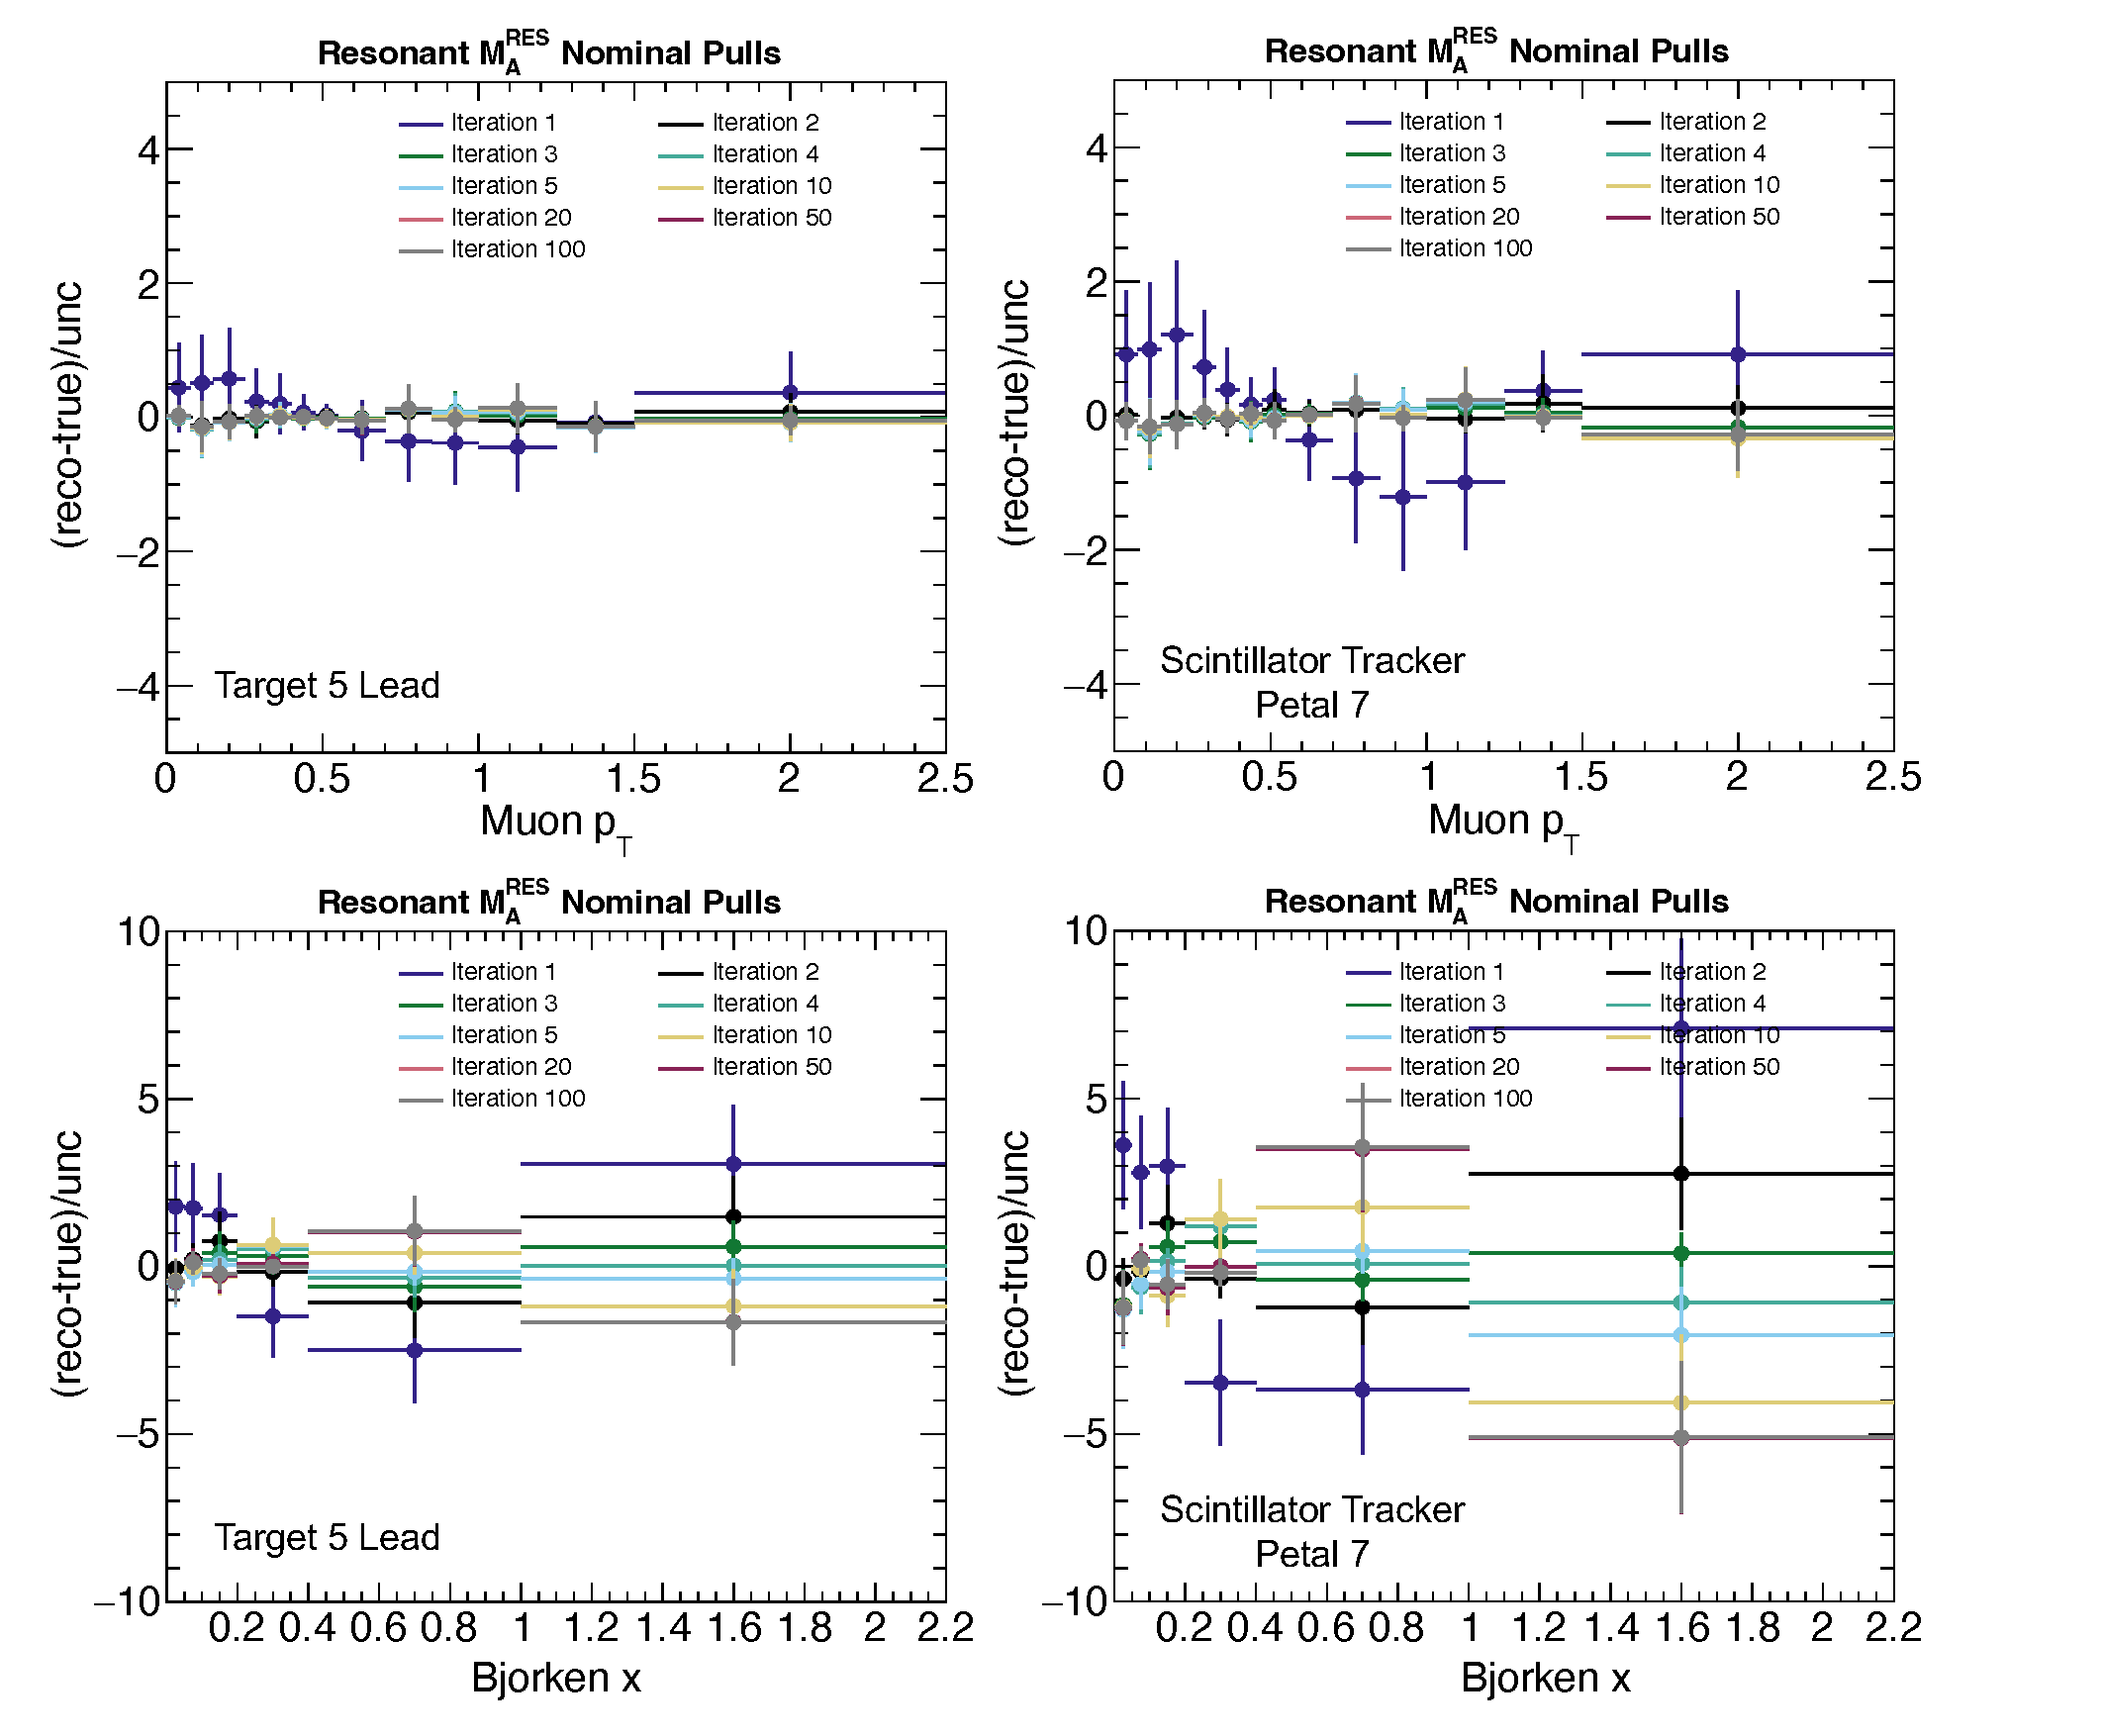
\includegraphics[width=0.95\textwidth]{07analysis1D/figures/maresWarp_lead5tracker7_pTx_pulls.pdf}}%
    \caption{Pull distributions for the 'Resonant $M_{A}^{\text{RES}}$ nominal' warping study are presented for target 5 lead (left panel) and the scintillator tracker petal 7 (right panel) in both antimuon $p_{\text{T}}$ (top) and Bjorken $x$ (bottom). In the case of $p_{\text{T}}$, both pull distributions illustrate a reduction in bias with each iteration of the unfolding process. However, for the Bjorken $x$ pull distribution, especially at high Bjorken $x$, there is an indication of some divergence, which prompted further investigation into potential model dependence.}
    %[short caption] {long caption}
    \label{fig:warpingMaRes_pulls}
\end{figure}

\begin{figure}[b!] 
    \centering
    {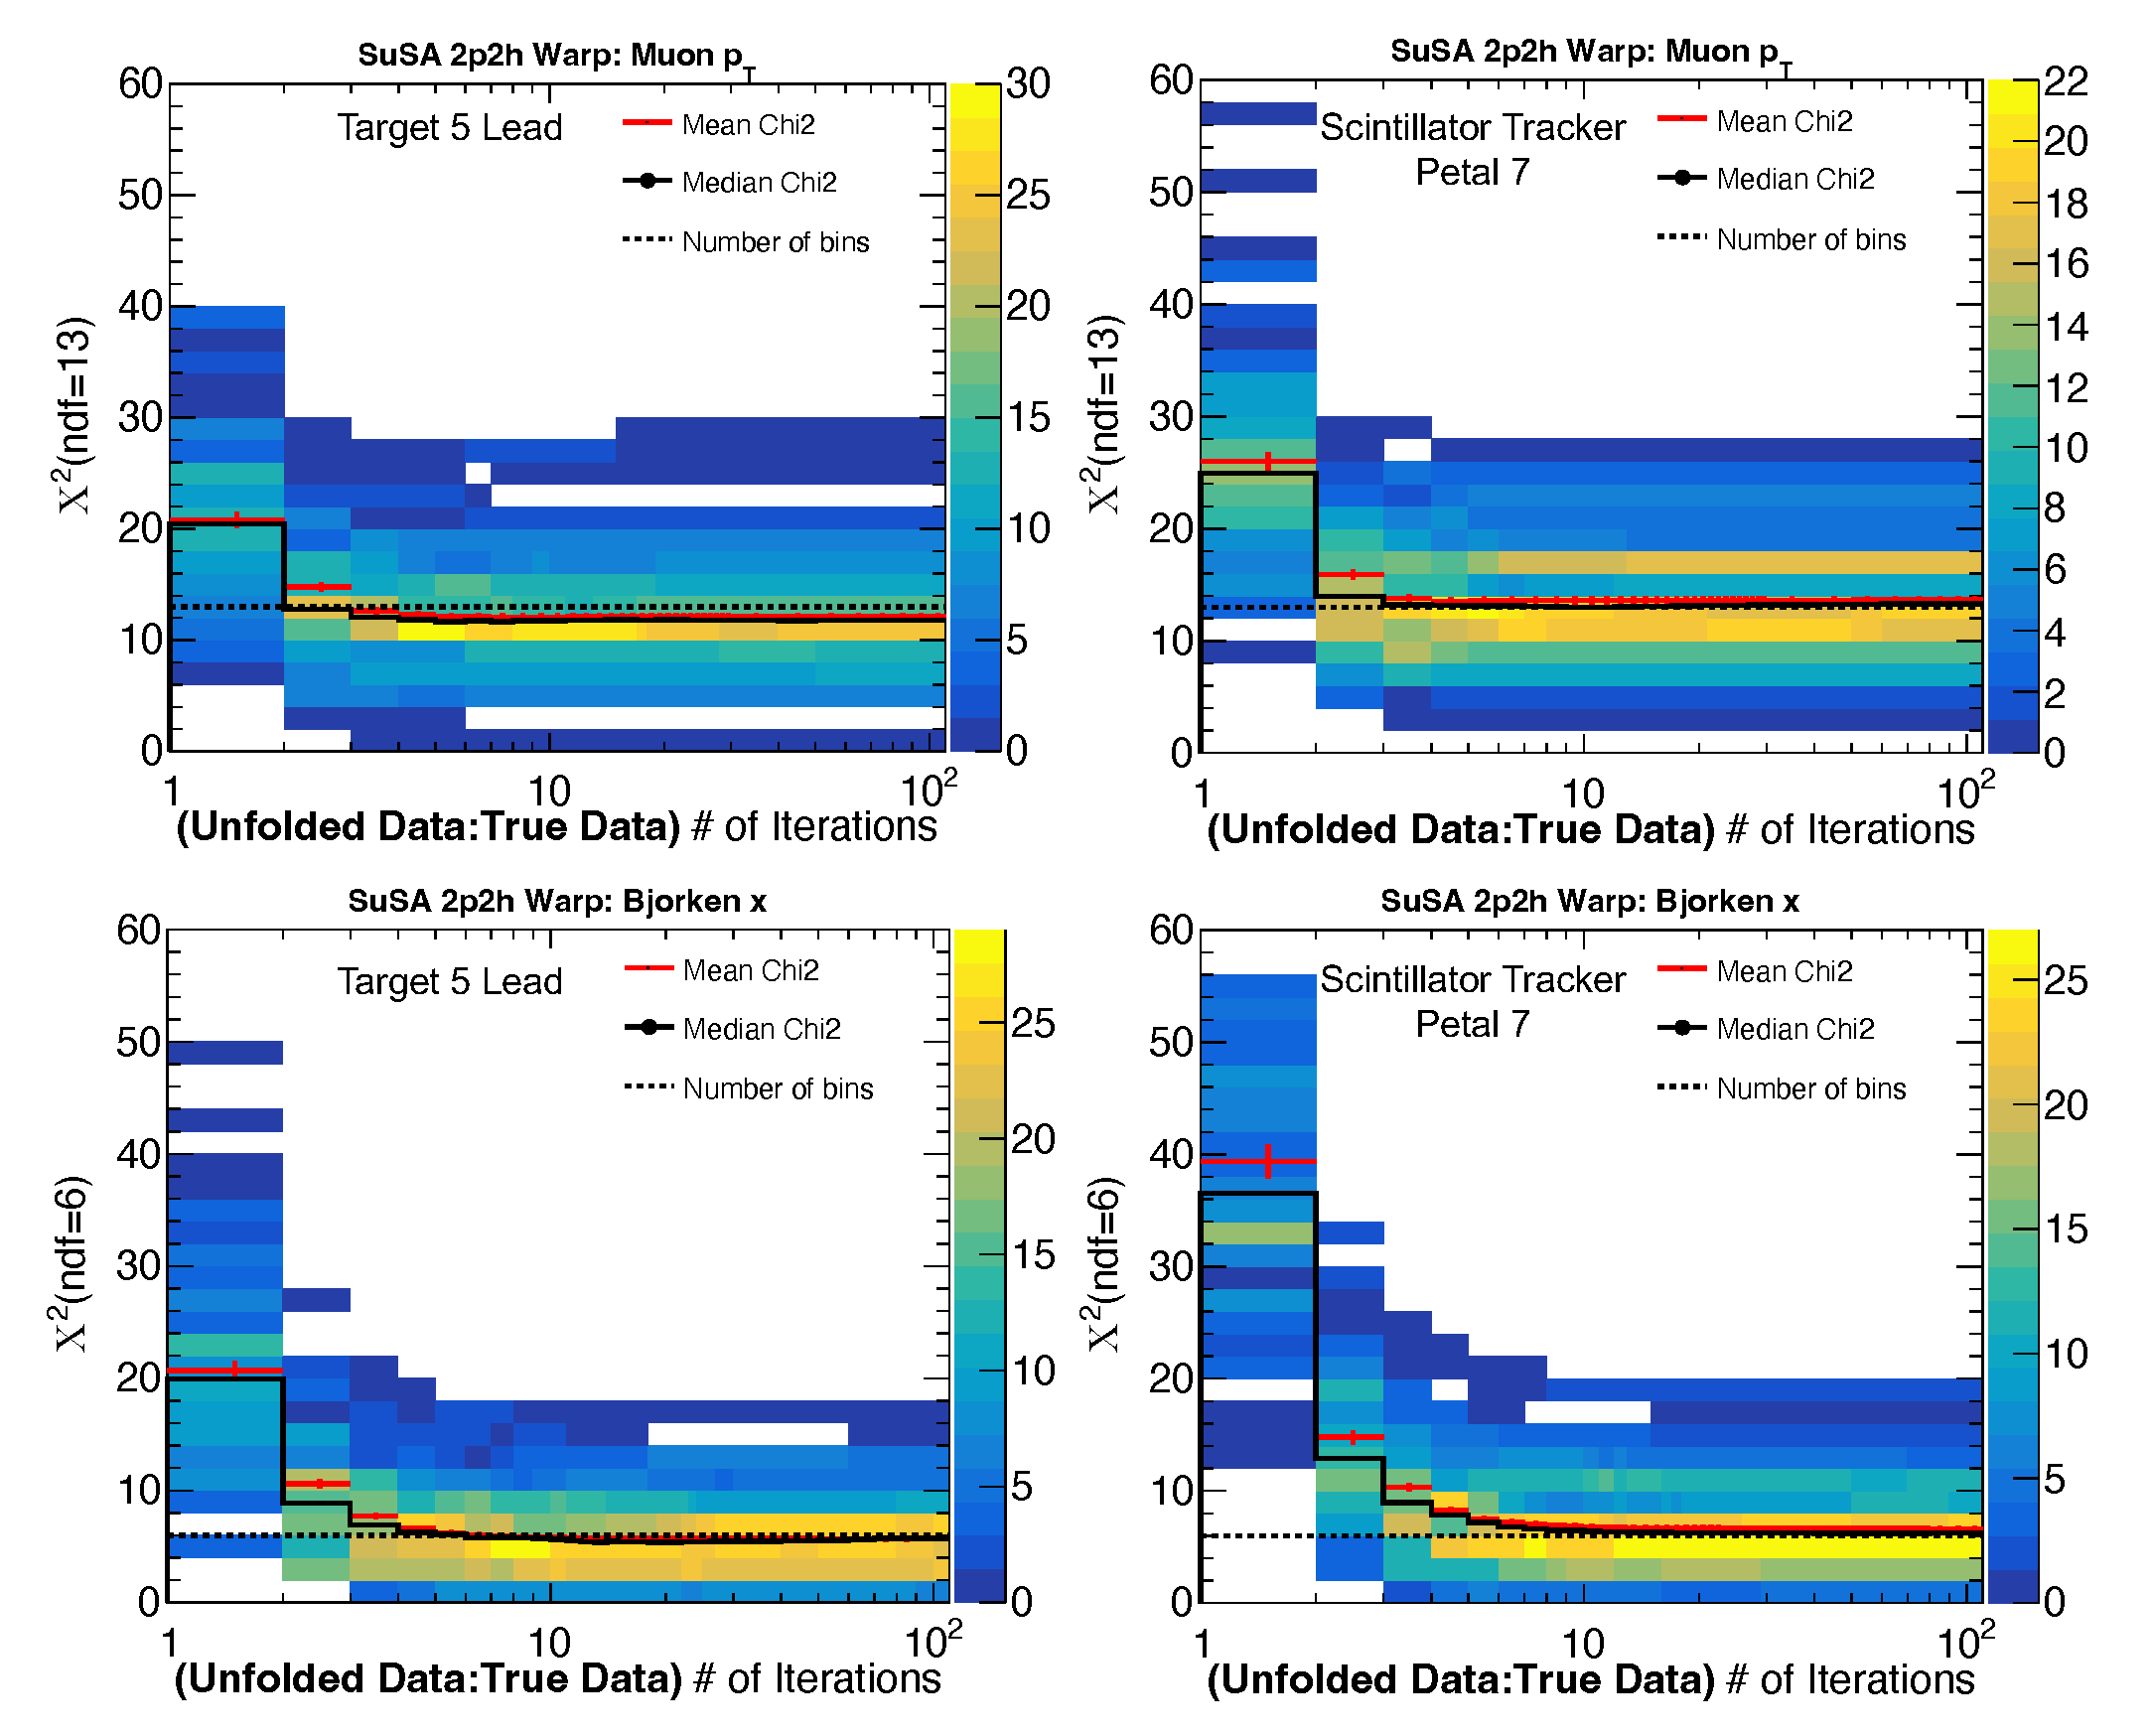
\includegraphics[width=1\textwidth]{07analysis1D/figures/susaWarp_lead5tracker7_pTx.pdf}}%
    \caption{The 'SuSA 2p2h' warping study conducted for target 5 lead (left panel) and the scintillator tracker petal 7 (right panel) in both antimuon $p_{\text{T}}$ (top) and Bjorken $x$ (bottom). Each heatmap displays the calculated $\chi^2$ between the unfolded and true distribution of the warped model as a function of the number of iterations for each of the 100 Poisson throws. The solid lines represent the median and mean $\chi^2$, while the dashed line indicates the number of bins or degrees of freedom (ndf). Both in $p_{\text{T}}$ and Bjorken $x$, the median $\chi^2$ stabilises at the ndf after several iterations indicating minimal bias.}
    %[short caption] {long caption}
    \label{fig:warpingSuSA}
\end{figure}

\begin{figure}%
    \vspace{-25pt}
    \centering
    \subfloat{{\includegraphics[width=0.5\textwidth]{thesisFigures/warpingStudies/MaRESwarp_xsec_check/crossSection_Daisy_t3_z06_x_minervame5A6A6B6C6D6E6F6G6H6I6J_DifferentCVComparison_Data.pdf} }}%
    \qquad
    \hspace{-40pt}
    \subfloat{{\includegraphics[width=0.5\textwidth]{thesisFigures/warpingStudies/MaRESwarp_xsec_check/crossSection_Daisy_t235_z26_x_minervame5A6A6B6C6D6E6F6G6H6I6J_DifferentCVComparison_Data.pdf} }}%
    \qquad
    \subfloat{{\includegraphics[width=0.5\textwidth]{thesisFigures/warpingStudies/MaRESwarp_xsec_check/crossSection_Daisy_t2345_z82_x_minervame5A6A6B6C6D6E6F6G6H6I6J_DifferentCVComparison_Data.pdf} }}%
    \qquad
    \hspace{-40pt}
    \subfloat{{\includegraphics[width=0.5\textwidth]{thesisFigures/warpingStudies/MaRESwarp_xsec_check/crossSection_t99_z99_x_minervame5A6A6B6C6D6E6F6G6H6I6J_DiffrentCVComparison_Data.pdf} }}%
    \caption{Comparison of the data cross-section for carbon (top left), iron (top right), lead (bottom left) and scintillator (bottom right) as a function of Bjorken $x$ extracted with the original simulation and `Resonant $M_{A}^{\text{RES}}$ nominal' central value to investigate potential model dependence.}
    %\vspace{0pt}}%
    \centering
    \subfloat{{\includegraphics[width=0.5\textwidth]{thesisFigures/warpingStudies/MaRESwarp_xsec_check/xSec_ratio_Daisy_t3_z06_x_minervame5A6A6B6C6D6E6F6G6H6I6J_DifferentCVComparison_Data.png} }}%
    \qquad
    \hspace{-40pt}
    \subfloat{{\includegraphics[width=0.5\textwidth]{thesisFigures/warpingStudies/MaRESwarp_xsec_check/xSec_ratio_Daisy_t235_z26_x_minervame5A6A6B6C6D6E6F6G6H6I6J_DifferentCVComparison_Data.pdf} }}%
    \caption{Comparison of the carbon-to-scintillator (left) and iron-to-scintillator (right) data cross-section ratio as a function of Bjorken $x$ extracted with the original simulation and `Resonant $M_{A}^{\text{RES}}$ nominal' central value. The central values of the data cross-section extracted using the warped model are encompassed by the total uncertainty (including the systematic, represented by the outer error bars) of the data cross-section extracted using the original simulation. This indicates that any potential model dependence is covered by the underlying uncertainty.}%
\end{figure}

\begin{figure}%
    \centering
    \subfloat{{\includegraphics[width=0.5\textwidth]{thesisFigures/warpingStudies/invisibleEnergyVariation/crossSection_Daisy_t3_z06_x_minervame5A6A6B6C6D6E6F6G6H6I6J_InvisibleEnergyVariation_Data.pdf} }}%
    \qquad
    \hspace{-40pt}
    \subfloat{{\includegraphics[width=0.5\textwidth]{thesisFigures/warpingStudies/invisibleEnergyVariation/crossSection_Daisy_t235_z26_x_minervame5A6A6B6C6D6E6F6G6H6I6J_InvisibleEnergyVariation_Data.pdf} }}%
    \qquad
    \subfloat{{\includegraphics[width=0.5\textwidth]{thesisFigures/warpingStudies/invisibleEnergyVariation/crossSection_Daisy_t2345_z82_x_minervame5A6A6B6C6D6E6F6G6H6I6J_InvisibleEnergyVariation_Data.pdf} }}%
    \qquad
    \hspace{-40pt}
    \subfloat{{\includegraphics[width=0.5\textwidth]{thesisFigures/warpingStudies/invisibleEnergyVariation/crossSection_t99_z99_x_minervame5A6A6B6C6D6E6F6G6H6I6J_InvisibleEnergyVariation_Data.pdf} }}%
    \caption{Comparison of the data cross-section for carbon (top left), iron (top right), lead (bottom left) and scintillator (bottom right) as a function of Bjorken $x$ extracted with the original simulation and `Invisible energy 10\%' central value to investigate model dependence arising from neutron modelling.}%
    \centering
    \subfloat{{\includegraphics[width=0.5\textwidth]{thesisFigures/warpingStudies/invisibleEnergyVariation/xSec_ratio_Daisy_t3_z06_x_minervame5A6A6B6C6D6E6F6G6H6I6J_InvisibleEnergyVariation_Data.pdf} }}%
    \qquad
    \hspace{-40pt}
    \subfloat{{\includegraphics[width=0.5\textwidth]{thesisFigures/warpingStudies/invisibleEnergyVariation/xSec_ratio_Daisy_t235_z26_x_minervame5A6A6B6C6D6E6F6G6H6I6J_InvisibleEnergyVariation_Data.pdf} }}%
    \caption{Comparison of the carbon-to-scintillator (left) and iron-to-scintillator (right) data cross-section ratio as a function of Bjorken $x$ extracted with the original simulation and `Invisible energy 10\%' central value to investigate model dependence arising from neutron modelling, revealing possible bias in the $x > 1$ bin.}%
\end{figure}
\vspace{-50pt}
\begin{figure}%
    \centering
    \subfloat{{\includegraphics[width=0.5\textwidth]{thesisFigures/warpingStudies/additionalStatUnc/Warping_t5_z82_minervame5A6A6B6C6D6E6F6G6H6I6J_cv_x_fStudy.pdf} }}%
    \qquad
    \hspace{-40pt}
    \subfloat{{\includegraphics[width=0.5\textwidth]{thesisFigures/warpingStudies/additionalStatUnc/Warping_t99_z99_minervame5A6A6B6C6D6E6F6G6H6I6J_cv_x_7_fStudy.pdf} }}%
    \caption{Correction factor $F$ to the statistical uncertainty of the unfolded sample due to finite size of the simulation in the migration matrix for target 5 lead and the scintillator tracker petal 7 in Bjorken $x$. The solid lines illustrate that at the selected number of iterations, i.e. 9 iterations, the calculated $\chi^2$ between the unfolded and true simulation converges to the number of degrees of freedom (dashed line) for the $F$ factor 4 and 4.5 for target 5 lead and the scintillator tracker petal 7 respectively.}%
\end{figure}


\clearpage
\thispagestyle{empty}
\hfill
\clearpage
\chapter{Unfolded distributions}

\label{ch:appendix_unfoldedDistributions}
\vspace{-10pt}
This appendix presents additional unfolded distributions not shown in Section~\ref{sec:migration_unfolding}, along with their associated fractional uncertainty breakdowns on the data. Specifically, it includes the unfolded distribution plots for target 2 iron and lead, target 3 carbon, iron, and lead, target 4 lead, and target 5 iron in both antimuon $p_{\text{T}}$ and Bjorken $x$.\enlargethispage{2\baselineskip}

\begin{figure}[h]%
    \centering
    \subfloat{{\includegraphics[width=0.49\textwidth]{thesisFigures/1Danalysis/Unfolded/unfolded_Daisy_t2_z26_pTmu1D_minervame5A6A6B6C6D6E6F6G6H6I6J.pdf} }}%
    \qquad
    \hspace{-50pt}
    \subfloat{{\includegraphics[width=0.49\textwidth]{thesisFigures/1Danalysis/Unfolded/unfolded_Daisy_t2_z26_x_minervame5A6A6B6C6D6E6F6G6H6I6J.pdf} }}%
    \caption{Unfolded distributions in antimuon $p_{\text{T}}$~(left) and Bjorken~$x$~(right) for target~2~iron. In the top panel, the pink band on the simulation represents the statistical uncertainty of the simulation. The data points carry both statistical (inner error bar) and systematic (outer error bar, which is the sum of statistical and systematic errors) uncertainties. The bottom panel of each plot displays the data-to-simulation ratio, with the pink band around 1 representing systematic uncertainty on the data, while the black points reflect the statistical uncertainty on the data-to-simulation ratio.}%
\end{figure}


\begin{figure}[h]%
    \vspace{-30pt}
    \centering
    \subfloat{{\includegraphics[width=0.49\textwidth]{thesisFigures/1Danalysis/Unfolded/unfolded_Daisy_t2_z82_pTmu1D_minervame5A6A6B6C6D6E6F6G6H6I6J.pdf} }}%
    \qquad
    \hspace{-50pt}
    \subfloat{{\includegraphics[width=0.49\textwidth]{thesisFigures/1Danalysis/Unfolded/unfolded_Daisy_t2_z82_x_minervame5A6A6B6C6D6E6F6G6H6I6J.pdf} }}%
    \caption{Unfolded distributions in antimuon $p_{\text{T}}$~(left) and Bjorken~$x$~(right) for target~2~lead. }%
    \vspace{-10pt}
    \subfloat{{\includegraphics[width=0.49\textwidth]{thesisFigures/1Danalysis/Unfolded/unfolded_Daisy_t3_z06_pTmu1D_minervame5A6A6B6C6D6E6F6G6H6I6J.pdf} }}%
    \qquad
    \hspace{-50pt}
    \subfloat{{\includegraphics[width=0.49\textwidth]{thesisFigures/1Danalysis/Unfolded/unfolded_Daisy_t3_z06_x_minervame5A6A6B6C6D6E6F6G6H6I6J.pdf} }}%
    \vspace{-10pt}
    \qquad
    \subfloat{{\includegraphics[width=0.49\textwidth]{thesisFigures/1Danalysis/Unfolded/unfolded_Daisy_t3_z26_pTmu1D_minervame5A6A6B6C6D6E6F6G6H6I6J.pdf} }}%
    \qquad
    \hspace{-50pt}
    \subfloat{{\includegraphics[width=0.49\textwidth]{thesisFigures/1Danalysis/Unfolded/unfolded_Daisy_t3_z26_x_minervame5A6A6B6C6D6E6F6G6H6I6J.pdf} }}%
    \caption{Unfolded distributions in antimuon $p_{\text{T}}$~(left panel) and Bjorken~$x$~(right panel) for target~3~carbon (top) and target~3~iron (bottom). }%
\end{figure}

\begin{figure}[t!]%
    \vspace{-30pt}
    \centering
    \subfloat{{\includegraphics[width=0.51\textwidth]{thesisFigures/1Danalysis/Unfolded/unfolded_Daisy_t3_z82_pTmu1D_minervame5A6A6B6C6D6E6F6G6H6I6J.pdf} }}%
    \qquad
    \hspace{-50pt}
    \subfloat{{\includegraphics[width=0.51\textwidth]{thesisFigures/1Danalysis/Unfolded/unfolded_Daisy_t3_z82_x_minervame5A6A6B6C6D6E6F6G6H6I6J.pdf} }}%
    \caption{Unfolded distributions in antimuon $p_{\text{T}}$~(left) and Bjorken~$x$~(right) for target~3~lead.}%
    \vspace{30pt}
    \subfloat{{\includegraphics[width=0.51\textwidth]{thesisFigures/1Danalysis/Unfolded/unfolded_Daisy_t4_z82_pTmu1D_minervame5A6A6B6C6D6E6F6G6H6I6J.pdf} }}%
    \qquad
    \hspace{-50pt}
    \subfloat{{\includegraphics[width=0.51\textwidth]{thesisFigures/1Danalysis/Unfolded/unfolded_Daisy_t4_z82_x_minervame5A6A6B6C6D6E6F6G6H6I6J.pdf} }}%
    \caption{Unfolded distributions in antimuon $p_{\text{T}}$~(left) and Bjorken~$x$~(right) for target~4~lead.}%
\end{figure}

\begin{figure}[h]%
    \vspace{-30pt}
    \subfloat{{\includegraphics[width=0.51\textwidth]{thesisFigures/1Danalysis/Unfolded/unfolded_Daisy_t5_z26_pTmu1D_minervame5A6A6B6C6D6E6F6G6H6I6J.pdf} }}%
    \qquad
    \hspace{-50pt}
    \subfloat{{\includegraphics[width=0.51\textwidth]{thesisFigures/1Danalysis/Unfolded/unfolded_Daisy_t5_z26_x_minervame5A6A6B6C6D6E6F6G6H6I6J.pdf} }}%
    \caption{Unfolded distributions in antimuon $p_{\text{T}}$~(left) and Bjorken~$x$~(right) for target~5~iron.}
    \subfloat{{\includegraphics[width=0.51\textwidth]{thesisFigures/1Danalysis/Unfolded/unfolded_FracErr_t2_z26_pTmu1D_minervame5A6A6B6C6D6E6F6G6H6I6J.pdf} }}%
    \qquad
    \hspace{-50pt}
    \subfloat{{\includegraphics[width=0.51\textwidth]{thesisFigures/1Danalysis/Unfolded/unfolded_FracErr_t2_z26_x_minervame5A6A6B6C6D6E6F6G6H6I6J.pdf} }}%
    \vspace{-10pt}
    \qquad
    \subfloat{{\includegraphics[width=0.51\textwidth]{thesisFigures/1Danalysis/Unfolded/unfolded_FracErr_t2_z82_pTmu1D_minervame5A6A6B6C6D6E6F6G6H6I6J.pdf} }}%
    \qquad
    \hspace{-50pt}
    \subfloat{{\includegraphics[width=0.51\textwidth]{thesisFigures/1Danalysis/Unfolded/unfolded_FracErr_t2_z82_x_minervame5A6A6B6C6D6E6F6G6H6I6J.pdf} }}
    \caption{Fractional uncertainty breakdowns on the unfolded data distributions in both~$p_{\text{T}}$ (left panel) and Bjorken $x$ (right panel) for target~2~iron~(top) and target~2~lead~(bottom).  }%
\end{figure}

\begin{figure}[h]%
    \vspace{-20pt}
    \centering
    \subfloat{{\includegraphics[width=0.51\textwidth]{thesisFigures/1Danalysis/Unfolded/unfolded_FracErr_t3_z06_pTmu1D_minervame5A6A6B6C6D6E6F6G6H6I6J.pdf} }}%
    \qquad
    \hspace{-50pt}
    \subfloat{{\includegraphics[width=0.51\textwidth]{thesisFigures/1Danalysis/Unfolded/unfolded_FracErr_t3_z06_x_minervame5A6A6B6C6D6E6F6G6H6I6J.pdf} }}
    \qquad
    \subfloat{{\includegraphics[width=0.51\textwidth]{thesisFigures/1Danalysis/Unfolded/unfolded_FracErr_t3_z26_pTmu1D_minervame5A6A6B6C6D6E6F6G6H6I6J.pdf} }}%
    \qquad
    \hspace{-50pt}
    \subfloat{{\includegraphics[width=0.51\textwidth]{thesisFigures/1Danalysis/Unfolded/unfolded_FracErr_t3_z26_x_minervame5A6A6B6C6D6E6F6G6H6I6J.pdf} }}%
    \qquad 
    \subfloat{{\includegraphics[width=0.51\textwidth]{thesisFigures/1Danalysis/Unfolded/unfolded_FracErr_t3_z82_pTmu1D_minervame5A6A6B6C6D6E6F6G6H6I6J.pdf} }}%
    \qquad
    \hspace{-50pt}
    \subfloat{{\includegraphics[width=0.51\textwidth]{thesisFigures/1Danalysis/Unfolded/unfolded_FracErr_t3_z82_x_minervame5A6A6B6C6D6E6F6G6H6I6J.pdf} }}
    \caption{Fractional uncertainty breakdowns on the unfolded data distributions in both~$p_{\text{T}}$ (left panel) and Bjorken $x$ (right panel) for target 3 carbon (top), target 3 iron~(middle), and target 3 lead (bottom).}%
\end{figure}

\begin{figure}[h]%
    \vspace{-100pt}
    \centering
    \subfloat{{\includegraphics[width=0.51\textwidth]{thesisFigures/1Danalysis/Unfolded/unfolded_FracErr_t4_z82_pTmu1D_minervame5A6A6B6C6D6E6F6G6H6I6J.pdf} }}%
    \qquad
    \hspace{-50pt}
    \subfloat{{\includegraphics[width=0.51\textwidth]{thesisFigures/1Danalysis/Unfolded/unfolded_FracErr_t4_z82_x_minervame5A6A6B6C6D6E6F6G6H6I6J.pdf} }}
    \caption{Fractional uncertainty breakdowns on the unfolded data distributions in both~$p_{\text{T}}$ (left panel) and Bjorken $x$ (right panel) for target 4 lead.}
    \vspace{30pt}
    \subfloat{{\includegraphics[width=0.51\textwidth]{thesisFigures/1Danalysis/Unfolded/unfolded_FracErr_t5_z26_pTmu1D_minervame5A6A6B6C6D6E6F6G6H6I6J.pdf} }}%
    \qquad
    \hspace{-50pt}
    \subfloat{{\includegraphics[width=0.51\textwidth]{thesisFigures/1Danalysis/Unfolded/unfolded_FracErr_t5_z26_x_minervame5A6A6B6C6D6E6F6G6H6I6J.pdf} }}
    \caption{Fractional uncertainty breakdowns on the unfolded data distributions in both $p_{\text{T}}$ (left panel) and Bjorken $x$ (right panel) for target 5 iron.}%
\end{figure}




\chapter{Efficiency distributions}

\label{ch:appendix_efficiencyCorrection}
\vspace{-20pt}
\begin{figure}[hb]%
    \centering
    \subfloat{{\includegraphics[width=0.5\textwidth]{thesisFigures/1Danalysis/Efficiency/Efficiency_t3_z06_pTmu1D_minervame5A6A6B6C6D6E6F6G6H6I6J.pdf} }}%
    \qquad
    \hspace{-40pt}
    \subfloat{{\includegraphics[width=0.5\textwidth]{thesisFigures/1Danalysis/Efficiency/Efficiency_t3_z06_x_minervame5A6A6B6C6D6E6F6G6H6I6J.pdf} }}%
    \caption{Efficiency correction distributions for target 3 carbon as a function of $p_{\text{T}}$ (left) and Bjorken $x$ (right).}%
\end{figure}
\vspace{-20pt}
\begin{figure}[hb]%
    \centering
    \subfloat{{\includegraphics[width=0.5\textwidth]{thesisFigures/1Danalysis/Efficiency/Efficiency_t3_z06_pTmu1D_minervame5A6A6B6C6D6E6F6G6H6I6J_FracErr.pdf} }}%
    \qquad
    \hspace{-40pt}
    \subfloat{{\includegraphics[width=0.5\textwidth]{thesisFigures/1Danalysis/Efficiency/Efficiency_t3_z06_x_minervame5A6A6B6C6D6E6F6G6H6I6J_FracErr.pdf} }}%
    \caption{Fractional uncertainty breakdown for the efficiency correction distributions for target 3 carbon as a function of $p_{\text{T}}$ (left) and Bjorken $x$ (right).}%
\end{figure}
\vspace{-20pt}
\begin{figure}[hb]
    \centering
    \subfloat{{\includegraphics[width=0.5\textwidth]{thesisFigures/1Danalysis/Efficiency/Efficiency_t235_z26_pTmu1D_minervame5A6A6B6C6D6E6F6G6H6I6J.pdf} }}%
    \qquad
    \hspace{-40pt}
    \subfloat{{\includegraphics[width=0.5\textwidth]{thesisFigures/1Danalysis/Efficiency/Efficiency_t235_z26_x_minervame5A6A6B6C6D6E6F6G6H6I6J.pdf} }}%
    \caption{Efficiency correction distributions for targets 2, 3, and 5 iron as a function of $p_{\text{T}}$ (left) and Bjorken $x$ (right).}%
\end{figure}
\vspace{-20pt}
\begin{figure}[hb]%
    \centering
    \subfloat{{\includegraphics[width=0.5\textwidth]{thesisFigures/1Danalysis/Efficiency/Efficiency_t2_z26_pTmu1D_minervame5A6A6B6C6D6E6F6G6H6I6J_FracErr.pdf} }}%
    \qquad
    \hspace{-40pt}
    \subfloat{{\includegraphics[width=0.5\textwidth]{thesisFigures/1Danalysis/Efficiency/Efficiency_t2_z26_x_minervame5A6A6B6C6D6E6F6G6H6I6J_FracErr.pdf} }}%
    \qquad
    \subfloat{{\includegraphics[width=0.5\textwidth]{thesisFigures/1Danalysis/Efficiency/Efficiency_t3_z26_pTmu1D_minervame5A6A6B6C6D6E6F6G6H6I6J_FracErr.pdf} }}%
    \qquad
    \hspace{-40pt}
    \subfloat{{\includegraphics[width=0.5\textwidth]{thesisFigures/1Danalysis/Efficiency/Efficiency_t3_z26_x_minervame5A6A6B6C6D6E6F6G6H6I6J_FracErr.pdf} }}%
    \caption{Fractional uncertainty breakdown for the efficiency correction distributions for targets 2 and 3 iron as a function of $p_{\text{T}}$ (left) and Bjorken $x$ (right).}%
\end{figure}
\vspace{-100pt}
\begin{figure}
    \centering
    \vspace{-10pt}
    \subfloat{{\includegraphics[width=0.5\textwidth]{thesisFigures/1Danalysis/Efficiency/Efficiency_t5_z26_pTmu1D_minervame5A6A6B6C6D6E6F6G6H6I6J_FracErr.pdf} }}%
    \qquad
    \hspace{-40pt}
    \subfloat{{\includegraphics[width=0.5\textwidth]{thesisFigures/1Danalysis/Efficiency/Efficiency_t5_z26_x_minervame5A6A6B6C6D6E6F6G6H6I6J_FracErr.pdf} }}%
    \caption{Fractional uncertainty breakdown for the efficiency correction distributions for target 5 iron as a function of $p_{\text{T}}$ (left) and Bjorken $x$ (right).}%
\end{figure}
\vspace{-40pt}
\begin{figure}
    \centering
    \vspace{-10pt}
    \subfloat{{\includegraphics[width=0.5\textwidth]{thesisFigures/1Danalysis/Efficiency/Efficiency_t2345_z82_pTmu1D_minervame5A6A6B6C6D6E6F6G6H6I6J.pdf} }}%
    \qquad
    \hspace{-40pt}
    \subfloat{{\includegraphics[width=0.5\textwidth]{thesisFigures/1Danalysis/Efficiency/Efficiency_t2345_z82_x_minervame5A6A6B6C6D6E6F6G6H6I6J.pdf} }}%
    \caption{Efficiency correction distributions for target 2--5 lead as a function of $p_{\text{T}}$ (left) and Bjorken $x$ (right).}%
\end{figure}
\vspace{-40pt}
\begin{figure}
    \centering
    \vspace{-10pt}
    \subfloat{{\includegraphics[width=0.5\textwidth]{thesisFigures/1Danalysis/Efficiency/Efficiency_t2_z82_pTmu1D_minervame5A6A6B6C6D6E6F6G6H6I6J_FracErr.pdf} }}%
    \qquad
    \hspace{-40pt}
    \subfloat{{\includegraphics[width=0.5\textwidth]{thesisFigures/1Danalysis/Efficiency/Efficiency_t2_z82_x_minervame5A6A6B6C6D6E6F6G6H6I6J_FracErr.pdf} }}%
    \caption{Fractional uncertainty breakdown for the efficiency correction distributions for target 2 lead as a function of $p_{\text{T}}$ (left) and Bjorken $x$ (right).}%
\end{figure}

\vspace{-20pt}
\begin{figure}[hb]%
    \centering
    \vspace{-40pt}
    \subfloat{{\includegraphics[width=0.5\textwidth]{thesisFigures/1Danalysis/Efficiency/Efficiency_t3_z82_pTmu1D_minervame5A6A6B6C6D6E6F6G6H6I6J_FracErr.pdf} }}%
    \qquad
    \hspace{-40pt}
    \subfloat{{\includegraphics[width=0.5\textwidth]{thesisFigures/1Danalysis/Efficiency/Efficiency_t3_z82_x_minervame5A6A6B6C6D6E6F6G6H6I6J_FracErr.pdf} }}%
    \qquad
    \subfloat{{\includegraphics[width=0.5\textwidth]{thesisFigures/1Danalysis/Efficiency/Efficiency_t4_z82_pTmu1D_minervame5A6A6B6C6D6E6F6G6H6I6J_FracErr.pdf} }}%
    \qquad
    \hspace{-40pt}
    \subfloat{{\includegraphics[width=0.5\textwidth]{thesisFigures/1Danalysis/Efficiency/Efficiency_t4_z82_x_minervame5A6A6B6C6D6E6F6G6H6I6J_FracErr.pdf} }}%
    \qquad
    \subfloat{{\includegraphics[width=0.5\textwidth]{thesisFigures/1Danalysis/Efficiency/Efficiency_t5_z82_pTmu1D_minervame5A6A6B6C6D6E6F6G6H6I6J_FracErr.pdf} }}%
    \qquad
    \hspace{-40pt}
    \subfloat{{\includegraphics[width=0.5\textwidth]{thesisFigures/1Danalysis/Efficiency/Efficiency_t5_z82_x_minervame5A6A6B6C6D6E6F6G6H6I6J_FracErr.pdf} }}%
    \caption{Fractional uncertainty breakdown for the efficiency correction distributions for targets 3--5 lead as a function of $p_{\text{T}}$ (left) and Bjorken $x$ (right).}%
\end{figure}
\vspace{-30pt}
\begin{figure}[ht]
    \centering
    \vspace{-10pt}
    \subfloat{{\includegraphics[width=0.5\textwidth]{thesisFigures/1Danalysis/Efficiency/Efficiency_t99_z99_pTmu1D_minervame5A6A6B6C6D6E6F6G6H6I6J.pdf} }}%
    \qquad
    \hspace{-40pt}
    \subfloat{{\includegraphics[width=0.5\textwidth]{thesisFigures/1Danalysis/Efficiency/Efficiency_t99_z99_x_minervame5A6A6B6C6D6E6F6G6H6I6J.pdf} }}%
    \caption{Efficiency correction distributions for the scintillator tracker as a function of $p_{\text{T}}$ (left) and Bjorken $x$ (right).}%
\end{figure}
\begin{figure}
    \centering
    \vspace{-10pt}
    \subfloat{{\includegraphics[width=0.5\textwidth]{thesisFigures/1Danalysis/Efficiency/Efficiency_t99_z99_pTmu1D_minervame5A6A6B6C6D6E6F6G6H6I6J_FracErr.pdf} }}%
    \qquad
    \hspace{-40pt}
    \subfloat{{\includegraphics[width=0.5\textwidth]{thesisFigures/1Danalysis/Efficiency/Efficiency_t99_z99_x_minervame5A6A6B6C6D6E6F6G6H6I6J_FracErr.pdf} }}%
    \caption{Fractional uncertainty breakdown for the efficiency correction distributions for the scintillator tracker as a function of $p_{\text{T}}$ (left) and Bjorken $x$ (right).}%
\end{figure}
\vspace{-30pt}
\begin{figure}
    \centering
    \vspace{-10pt}
    \subfloat{{\includegraphics[width=0.5\textwidth]{thesisFigures/1Danalysis/Efficiency/Efficiency_daisy_t99_z99_pTmu1D_minervame5A6A6B6C6D6E6F6G6H6I6J.pdf} }}%
    \qquad
    \hspace{-40pt}
    \subfloat{{\includegraphics[width=0.5\textwidth]{thesisFigures/1Danalysis/Efficiency/Efficiency_daisy_t99_z99_x_minervame5A6A6B6C6D6E6F6G6H6I6J.pdf} }}%
    \caption{Efficiency correction distributions for the scintillator tracker in ‘daisy petals' as a function of $p_{\text{T}}$ (left) and Bjorken $x$ (right).}%
\end{figure}




\clearpage
\thispagestyle{empty}
\hfill
\clearpage
\chapter{Efficiency-corrected distributions}

\label{ch:appendix_effCorrectedDistributions}


%%%%%%%%%%%%%%%%%%%%%%%%%%%%%%%%%%%%%%%%%%%%%%%
\vspace{-20pt}
This appendix presents the efficiency-corrected distributions per target and material combination not shown in Section~\ref{ch:efficiency}, along with their associated fractional uncertainty breakdowns on the data. Furthermore, the efficiency-corrected distributions in $p_{\text{T}}$ and Bjorken~$x$ combining targets 2, 3, and 5 iron are also included with their corresponding fractional uncertainties on the combined data distributions.\enlargethispage{2\baselineskip}

\begin{figure}[h]%
    \vspace{-13pt}
    \centering
    \subfloat{{\includegraphics[width=0.49\textwidth]{thesisFigures/1Danalysis/UnfoldedEffCorrected/unfolded_effCorrected_Daisy_t2_z26_pTmu1D_minervame5A6A6B6C6D6E6F6G6H6I6J.pdf} }}%
    \qquad
    \hspace{-50pt}
    \subfloat{{\includegraphics[width=0.49\textwidth]{thesisFigures/1Danalysis/UnfoldedEffCorrected/unfolded_effCorrected_Daisy_t2_z26_x_minervame5A6A6B6C6D6E6F6G6H6I6J.pdf} }}%
    \caption{Efficiency-corrected distributions in antimuon $p_{\text{T}}$~(left) and Bjorken~$x$~(right) for target~2~iron with the simulation broken down into the various interaction channels stacked in the descending order of their contribution. In the top panel, the pink band on the simulation represents the statistical uncertainty of the simulation. The data points carry both statistical (inner error bar) and systematic (outer error bar, which is the sum of statistical and systematic errors) uncertainties. The bottom panel of each plot displays the data-to-simulation ratio, with the pink band around 1 representing systematic uncertainty on the data, while the black points reflect the statistical uncertainty on the data-to-simulation ratio.}%
\end{figure}


\begin{figure}[h]%
    \vspace{-30pt}
    \centering
    \subfloat{{\includegraphics[width=0.49\textwidth]{thesisFigures/1Danalysis/UnfoldedEffCorrected/unfolded_effCorrected_Daisy_t2_z82_pTmu1D_minervame5A6A6B6C6D6E6F6G6H6I6J.pdf} }}%
    \qquad
    \hspace{-50pt}
    \subfloat{{\includegraphics[width=0.49\textwidth]{thesisFigures/1Danalysis/UnfoldedEffCorrected/unfolded_effCorrected_Daisy_t2_z82_x_minervame5A6A6B6C6D6E6F6G6H6I6J.pdf} }}%
    \caption{Efficiency-corrected distributions in antimuon $p_{\text{T}}$~(left) and Bjorken~$x$~(right) for target~2~lead. }%
    \vspace{-10pt}
    \subfloat{{\includegraphics[width=0.49\textwidth]{thesisFigures/1Danalysis/UnfoldedEffCorrected/unfolded_effCorrected_Daisy_t3_z06_pTmu1D_minervame5A6A6B6C6D6E6F6G6H6I6J.pdf} }}%
    \qquad
    \hspace{-50pt}
    \subfloat{{\includegraphics[width=0.49\textwidth]{thesisFigures/1Danalysis/UnfoldedEffCorrected/unfolded_effCorrected_Daisy_t3_z06_x_minervame5A6A6B6C6D6E6F6G6H6I6J.pdf} }}%
    \vspace{-10pt}
    \qquad
    \subfloat{{\includegraphics[width=0.49\textwidth]{thesisFigures/1Danalysis/UnfoldedEffCorrected/unfolded_effCorrected_Daisy_t3_z26_pTmu1D_minervame5A6A6B6C6D6E6F6G6H6I6J.pdf} }}%
    \qquad
    \hspace{-50pt}
    \subfloat{{\includegraphics[width=0.49\textwidth]{thesisFigures/1Danalysis/UnfoldedEffCorrected/unfolded_effCorrected_Daisy_t3_z26_x_minervame5A6A6B6C6D6E6F6G6H6I6J.pdf} }}%
    \caption{Efficiency-corrected distributions in antimuon $p_{\text{T}}$~(left panel) and Bjorken~$x$~(right panel) for target~3~carbon (top) and target~3~iron (bottom). }%
\end{figure}

\begin{figure}[t!]%
    \vspace{-30pt}
    \centering
    \subfloat{{\includegraphics[width=0.51\textwidth]{thesisFigures/1Danalysis/UnfoldedEffCorrected/unfolded_effCorrected_Daisy_t3_z82_pTmu1D_minervame5A6A6B6C6D6E6F6G6H6I6J.pdf} }}%
    \qquad
    \hspace{-50pt}
    \subfloat{{\includegraphics[width=0.51\textwidth]{thesisFigures/1Danalysis/UnfoldedEffCorrected/unfolded_effCorrected_Daisy_t3_z82_x_minervame5A6A6B6C6D6E6F6G6H6I6J.pdf} }}%
    \caption{Efficiency-corrected distributions in antimuon $p_{\text{T}}$~(left) and Bjorken~$x$~(right) for target~3~lead.}%
    \vspace{30pt}
    \subfloat{{\includegraphics[width=0.51\textwidth]{thesisFigures/1Danalysis/UnfoldedEffCorrected/unfolded_effCorrected_Daisy_t4_z82_pTmu1D_minervame5A6A6B6C6D6E6F6G6H6I6J.pdf} }}%
    \qquad
    \hspace{-50pt}
    \subfloat{{\includegraphics[width=0.51\textwidth]{thesisFigures/1Danalysis/UnfoldedEffCorrected/unfolded_effCorrected_Daisy_t4_z82_x_minervame5A6A6B6C6D6E6F6G6H6I6J.pdf} }}%
    \caption{Efficiency-corrected distributions in antimuon $p_{\text{T}}$~(left) and Bjorken~$x$~(right) for target~4~lead.}%
\end{figure}

\begin{figure}[h]%
    \vspace{-30pt}
    \subfloat{{\includegraphics[width=0.51\textwidth]{thesisFigures/1Danalysis/UnfoldedEffCorrected/unfolded_effCorrected_Daisy_t5_z26_pTmu1D_minervame5A6A6B6C6D6E6F6G6H6I6J.pdf} }}%
    \qquad
    \hspace{-50pt}
    \subfloat{{\includegraphics[width=0.51\textwidth]{thesisFigures/1Danalysis/UnfoldedEffCorrected/unfolded_effCorrected_Daisy_t5_z26_x_minervame5A6A6B6C6D6E6F6G6H6I6J.pdf} }}%
    \caption{Efficiency-corrected distributions in antimuon $p_{\text{T}}$~(left) and Bjorken~$x$~(right) for target~5~iron.}
    \subfloat{{\includegraphics[width=0.51\textwidth]{thesisFigures/1Danalysis/UnfoldedEffCorrected/unfolded_effCorrected_FracErr_t2_z26_pTmu1D_minervame5A6A6B6C6D6E6F6G6H6I6J.pdf} }}%
    \qquad
    \hspace{-50pt}
    \subfloat{{\includegraphics[width=0.51\textwidth]{thesisFigures/1Danalysis/UnfoldedEffCorrected/unfolded_effCorrected_FracErr_t2_z26_x_minervame5A6A6B6C6D6E6F6G6H6I6J.pdf} }}%
    \vspace{-10pt}
    \qquad
    \subfloat{{\includegraphics[width=0.51\textwidth]{thesisFigures/1Danalysis/UnfoldedEffCorrected/unfolded_effCorrected_FracErr_t2_z82_pTmu1D_minervame5A6A6B6C6D6E6F6G6H6I6J.pdf} }}%
    \qquad
    \hspace{-50pt}
    \subfloat{{\includegraphics[width=0.51\textwidth]{thesisFigures/1Danalysis/UnfoldedEffCorrected/unfolded_effCorrected_FracErr_t2_z82_x_minervame5A6A6B6C6D6E6F6G6H6I6J.pdf} }}
    \caption{Fractional uncertainty breakdowns on the efficiency-corrected data distributions in both~$p_{\text{T}}$ (left panel) and Bjorken $x$ (right panel) for target~2~iron~(top) and target~2~lead~(bottom).  }%
\end{figure}

\begin{figure}[h]%
    \vspace{-20pt}
    \centering
    \subfloat{{\includegraphics[width=0.51\textwidth]{thesisFigures/1Danalysis/UnfoldedEffCorrected/unfolded_effCorrected_FracErr_t3_z06_pTmu1D_minervame5A6A6B6C6D6E6F6G6H6I6J.pdf} }}%
    \qquad
    \hspace{-50pt}
    \subfloat{{\includegraphics[width=0.51\textwidth]{thesisFigures/1Danalysis/UnfoldedEffCorrected/unfolded_effCorrected_FracErr_t3_z06_x_minervame5A6A6B6C6D6E6F6G6H6I6J.pdf} }}
    \qquad
    \subfloat{{\includegraphics[width=0.51\textwidth]{thesisFigures/1Danalysis/UnfoldedEffCorrected/unfolded_effCorrected_FracErr_t3_z26_pTmu1D_minervame5A6A6B6C6D6E6F6G6H6I6J.pdf} }}%
    \qquad
    \hspace{-50pt}
    \subfloat{{\includegraphics[width=0.51\textwidth]{thesisFigures/1Danalysis/UnfoldedEffCorrected/unfolded_effCorrected_FracErr_t3_z26_x_minervame5A6A6B6C6D6E6F6G6H6I6J.pdf} }}%
    \qquad 
    \subfloat{{\includegraphics[width=0.51\textwidth]{thesisFigures/1Danalysis/UnfoldedEffCorrected/unfolded_effCorrected_FracErr_t3_z82_pTmu1D_minervame5A6A6B6C6D6E6F6G6H6I6J.pdf} }}%
    \qquad
    \hspace{-50pt}
    \subfloat{{\includegraphics[width=0.51\textwidth]{thesisFigures/1Danalysis/UnfoldedEffCorrected/unfolded_effCorrected_FracErr_t3_z82_x_minervame5A6A6B6C6D6E6F6G6H6I6J.pdf} }}
    \caption{Fractional uncertainty breakdowns on the efficiency-corrected data distributions in both~$p_{\text{T}}$ (left panel) and Bjorken $x$ (right panel) for target 3 carbon (top), target~3~iron~(middle), and target~3 lead (bottom).}%
\end{figure}

\begin{figure}[h]%
    \vspace{-100pt}
    \centering
    \subfloat{{\includegraphics[width=0.51\textwidth]{thesisFigures/1Danalysis/UnfoldedEffCorrected/unfolded_effCorrected_FracErr_t4_z82_pTmu1D_minervame5A6A6B6C6D6E6F6G6H6I6J.pdf} }}%
    \qquad
    \hspace{-50pt}
    \subfloat{{\includegraphics[width=0.51\textwidth]{thesisFigures/1Danalysis/UnfoldedEffCorrected/unfolded_effCorrected_FracErr_t4_z82_x_minervame5A6A6B6C6D6E6F6G6H6I6J.pdf} }}
    \caption{Fractional uncertainty breakdowns on the efficiency-corrected data distributions in both~$p_{\text{T}}$ (left panel) and Bjorken $x$ (right panel) for target 4 lead.}
    \vspace{30pt}
    \subfloat{{\includegraphics[width=0.51\textwidth]{thesisFigures/1Danalysis/UnfoldedEffCorrected/unfolded_effCorrected_FracErr_t5_z26_pTmu1D_minervame5A6A6B6C6D6E6F6G6H6I6J.pdf} }}%
    \qquad
    \hspace{-50pt}
    \subfloat{{\includegraphics[width=0.51\textwidth]{thesisFigures/1Danalysis/UnfoldedEffCorrected/unfolded_effCorrected_FracErr_t5_z26_x_minervame5A6A6B6C6D6E6F6G6H6I6J.pdf} }}
    \caption{Fractional uncertainty breakdowns on the efficiency-corrected data distributions in both $p_{\text{T}}$ (left panel) and Bjorken $x$ (right panel) for target 5 iron.}%
\end{figure}


\begin{figure}[h]%
    \vspace{-100pt}
    \centering
    \subfloat{{\includegraphics[width=0.51\textwidth]{thesisFigures/1Danalysis/UnfoldedEffCorrectedCombined/total_unfolded_effCorrected_Daisy_t235_z26_pTmu1D_minervame5A6A6B6C6D6E6F6G6H6I6J.pdf} }}%
    \qquad
    \hspace{-50pt}
    \subfloat{{\includegraphics[width=0.51\textwidth]{thesisFigures/1Danalysis/UnfoldedEffCorrectedCombined/total_unfolded_effCorrected_Daisy_t235_z26_x_minervame5A6A6B6C6D6E6F6G6H6I6J.pdf} }}
    \caption{Efficiency-corrected distributions in antimuon $p_{\text{T}}$~(left) and Bjorken~$x$~(right) for combined iron, i.e. combined target 2, 3, and 5 iron. }%
    \vspace{30pt}
    \subfloat{{\includegraphics[width=0.51\textwidth]{thesisFigures/1Danalysis/UnfoldedEffCorrectedCombined/total_unfolded_effCorrected_FracErr_t235_z26_pTmu1D_minervame5A6A6B6C6D6E6F6G6H6I6J.pdf} }}%
    \qquad
    \hspace{-50pt}
    \subfloat{{\includegraphics[width=0.51\textwidth]{thesisFigures/1Danalysis/UnfoldedEffCorrectedCombined/total_unfolded_effCorrected_FracErr_t235_z26_x_minervame5A6A6B6C6D6E6F6G6H6I6J.pdf} }}
    \caption{Fractional uncertainty breakdowns on the efficiency-corrected data distributions in both $p_{\text{T}}$ (left) and Bjorken $x$ (right) for combined iron, i.e. combined target 2, 3, and 5 iron.}%
\end{figure}

\clearpage
\thispagestyle{empty}
\hfill
\clearpage
\chapter{Fractional systematic uncertainties}

\label{ch:appendix_sysUncertainties}

\begin{figure}[hb]%
    \vspace{-45pt}
    \centering
    \subfloat{{\includegraphics[width=0.51\textwidth]{thesisFigures/1Danalysis/EventSelection_thesis/EventSelection_t99_z99_pTmu1D_minervame5A6A6B6C6D6E6F6G6H6I6J_FracErr_fixed.pdf} }}%
    \qquad
    \hspace{-47pt}
    \subfloat{{\includegraphics[width=0.51\textwidth]{thesisFigures/1Danalysis/EventSelection_thesis/EventSelection_t99_z99_x_minervame5A6A6B6C6D6E6F6G6H6I6J_FracErr_fixed.pdf} }}%
    \caption{Fractional uncertainty breakdown for the simulated event rate in both $p_{\text{T}}$~(left) and Bjorken~$x$ (right) in the scintillator tracker.}%
\end{figure}

\begin{figure}[hb]%
    \vspace{-17pt}
    \centering
    \subfloat{{\includegraphics[width=0.51\textwidth]{thesisFigures/systematics/crossSection_Daisy_FracErr_t2345_z82_x_minervame5A6A6B6C6D6E6F6G6H6I6J_muonReco.pdf} }}%
    \qquad
    \hspace{-50pt}
    \subfloat{{\includegraphics[width=0.51\textwidth]{thesisFigures/systematics/crossSection_FracErr_t99_z99_x_minervame5A6A6B6C6D6E6F6G6H6I6J_muonReco.pdf} }}%
    \caption{Breakdown of various sources of uncertainty in the `Muon Reconstruction' error band in the lead (left) and scintillator (right) differential cross-section in data in Bjorken $x$.}%
\end{figure}

\begin{figure}[t!]%
    \vspace{-480pt}
    \centering
    \subfloat{{\includegraphics[width=0.51\textwidth]{thesisFigures/systematics/crossSection_FracErr_t99_z99_x_minervame5A6A6B6C6D6E6F6G6H6I6J_intModel2.pdf} }}%
    \qquad
    \hspace{-50pt}
    \subfloat{{\includegraphics[width=0.51\textwidth]{thesisFigures/systematics/crossSection_FracErr_t99_z99_x_minervame5A6A6B6C6D6E6F6G6H6I6J_fsi2.pdf} }}%
    \caption{Close-up of the breakdowns of various sources of uncertainty in the `Interaction Model' (left) and the `FSI'  error band in the scintillator differential cross-section in data in Bjorken $x$.}%
\end{figure}
\chapter{MINERvA tune comparisons}

\label{ch:appendix_tuneComparisons}

This appendix presents the measured cross-section and cross-section ratio results compared to the various MINERvA tunes applied to the baseline GENIE 2.12.6 \cite{genie_ANDREOPOULOS201087,genie_andreopoulos2015}. These comparisons facilitate a broader understanding of this measurement in the context of other MINERvA results. The underlying simulation prediction corresponds to the MINERvA tune v4.3.0. In the comparisons, the baseline GENIE 2.12.6 is considered in addition to the so-called v1, v2 and v4 tunes based on different MINERvA results or reanalyses of other data. The characteristics of each tune are briefly reviewed below:
\begin{itemize}
    \item \textbf{GENIE 2.12.6}: baseline GENIE prediction
    \item \textbf{MINERvA tune v1}: GENIE 2.12.6 + Valencia RPA suppression of the quasi-elastic interactions~\cite{RPANieves2004_PhysRevC.70.055503, Rodrigues2016_PhysRevLett.116.071802, gran2017model}, enhanced 2p2h \cite{2p2hNieves2011_PhysRevC.83.045501,2p2hGran2013_PhysRevD.88.113007,2p2hschwehr2017genie,Rodrigues2016_PhysRevLett.116.071802, Gran2018_PhysRevLett.120.221805}, and reduced non-resonant pion production \cite{pion_Rodrigues_2016}
    \item \textbf{MINERvA tune v2}: v1 + low $Q^2$ suppression based on MINERvA's low-energy pion production data and older bubble chamber data \cite{PhysRevD.100.072005}
    \item \textbf{MINERvA tune v4}: v1 + full bubble chamber fit changing $M_{A}^{\text{RES}}$ and charged-current resonant normalisation parameter \cite{pion_Rodrigues_2016}
    \item \textbf{MINERvA tune v4.3.0}: v4 + low $Q^2$ suppression based on MINERvA's medium energy charged-current 1$\pi^+$ analysis \cite{Bercellie2023_PhysRevLett.131.011801}
\end{itemize}
Chapter~\ref{ch:dataAsimulation} provides a detailed description of the specific modifications made to the baseline GENIE predictions to create the MINERvA tune v4.3.0.

% pT xsec

\begin{figure}[t!]%
    \vspace{-20pt}
    \centering
    \subfloat{{\includegraphics[width=0.49\textwidth]{thesisFigures/tuneComparisons2024/crossSection_Daisy_t3_z06_pTmu1D_minervame5A6A6B6C6D6E6F6G6H6I6J_TuneComparison+ratio.pdf} }}%
    \qquad
    \hspace{-50pt}
    \subfloat{{\includegraphics[width=0.49\textwidth]{thesisFigures/tuneComparisons2024/crossSection_t99_z99_pTmu1D_minervame5A6A6B6C6D6E6F6G6H6I6J_TuneComparison+ratio.pdf} }}
    \vspace{-10pt}
    \qquad
    \subfloat{{\includegraphics[width=0.49\textwidth]{thesisFigures/tuneComparisons2024/crossSection_Daisy_t235_z26_pTmu1D_minervame5A6A6B6C6D6E6F6G6H6I6J_TuneComparison+ratio.pdf} }}%
    \qquad
    \hspace{-50pt}
    \subfloat{{\includegraphics[width=0.49\textwidth]{thesisFigures/tuneComparisons2024/crossSection_Daisy_t2345_z82_pTmu1D_minervame5A6A6B6C6D6E6F6G6H6I6J_TuneComparison+ratio.pdf} }}%
    \caption{Measured carbon, scintillator, iron, and lead (from left to right, top to bottom) cross-section as a function of antimuon $p_{\text{T}}$ compared to the predictions from different MINERvA tunes. The inner error bar on the data indicates the statistical error while the outer error bar corresponds to the total, i.e. statistical + systematic, error.}
\end{figure}

\begin{table}[b!]
    \vspace{-30pt}
    \centering
    \begin{tabular}{c c c c c c c }
    \hline \\ [-1.5 ex]
    \multirow[c]{2}{*}{Cross-section} & \multicolumn{5}{c}{MINERvA tune $\chi^2$/ndf for $p_{\text{T}}$ (ndf = 13) } \\ [0.8ex]
     & CV & GENIE 2.12.6 & v1 & v2 & v4   \\ [0.5ex] % inserts table %heading
    \hline
    \hline \\[-1.9ex]
    Carbon &  2.64 &	2.12 &	2.12 &	4.88 &	2.93  \\
    %\hline
    Iron & 3.04 &	9.30 &	7.06 &	4.81 &	11.48  \\
    %\hline
    Lead & 6.22	& 18.20	& 15.72 & 2.62 &	24.86  \\
    %\hline
    Scintillator & 10.35 & 42.07 &	24.89 &	39.29 &	51.82  \\
    \hline
    \end{tabular}

    \caption{Fully correlated $\chi^2$/ndf calculated according to Equation~\ref{eq:fullyCorrelatedChi2} to assess the agreement between the measured data and the various MINERvA tunes for carbon, scintillator, iron, and lead cross-section in antimuon $p_{\text{T}}$. }
    \label{table:xsec_tuneComparison_pT}
\end{table}

% pT ratio
\begin{figure}[t!]%
    \centering
    \subfloat{{\includegraphics[width=0.49\textwidth]{thesisFigures/tuneComparisons2024/xSec_ratio_Daisy_t3_z06_pTmu1D_minervame5A6A6B6C6D6E6F6G6H6I6J_TuneComparison.pdf} }}%
    \qquad
    \hspace{-50pt}
    \subfloat{{\includegraphics[width=0.49\textwidth]{thesisFigures/tuneComparisons2024/xSec_ratio_Daisy_t235_z26_pTmu1D_minervame5A6A6B6C6D6E6F6G6H6I6J_TuneComparison.pdf} }}
    \vspace{-10pt}
    \qquad
    \subfloat{{\includegraphics[width=0.49\textwidth]{thesisFigures/tuneComparisons2024/xSec_ratio_Daisy_t2345_z82_pTmu1D_minervame5A6A6B6C6D6E6F6G6H6I6J_TuneComparison.pdf} }}%
    \caption{Measured carbon-to-scintillator (top left), iron-to-scintillator (top right), and lead-to-scintillator (bottom) cross-section ratios in antimuon $p_{\text{T}}$ compared to the predictions from different MINERvA tunes. The data is displayed with both the statistical~(inner error bars) and the total (outer error bars) uncertainty.}
\end{figure}

\begin{table}[b!]
    \centering
    \begin{tabular}{c c c c c c c }
    \hline \\ [-1.5 ex]
    \multirow[c]{2}{*}{Cross-section ratio} & \multicolumn{5}{c}{MINERvA tune $\chi^2$/ndf for $p_{\text{T}}$ (ndf = 13) } \\ [0.8ex]
     & CV & GENIE 2.12.6 & v1 & v2 & v4   \\ [0.5ex] % inserts table %heading
    \hline
    \hline \\[-1.9ex]
    C/CH & 4.93 & 5.17 & 4.93 & 5.55 & 4.90 \\
    %\hline
    Fe/CH & 2.35 & 2.17 & 2.39 & 1.33 & 2.61  \\
    %\hline
    Pb/CH & 12.06 & 6.68 & 10.00 & 2.94 & 11.32  \\
    \hline
    \end{tabular}    
    \caption{Fully correlated $\chi^2$/ndf calculated according to Equation~\ref{eq:fullyCorrelatedChi2} to assess the agreement between the measured data and the various models in the cross-section ratios to scintillator for carbon, iron, and lead in antimuon $p_{\text{T}}$.}
    \label{table:xsecRatio_tuneComparison_pT}
\end{table}

% x sec

\begin{figure}[t!]%
    \vspace{-30pt}
    \centering
    \subfloat{{\includegraphics[width=0.49\textwidth]{thesisFigures/tuneComparisons2024/crossSection_Daisy_t3_z06_x_minervame5A6A6B6C6D6E6F6G6H6I6J_TuneComparison+ratio.pdf} }}%
    \qquad
    \hspace{-50pt}
    \subfloat{{\includegraphics[width=0.49\textwidth]{thesisFigures/tuneComparisons2024/crossSection_t99_z99_x_minervame5A6A6B6C6D6E6F6G6H6I6J_TuneComparison+ratio.pdf} }}
    \vspace{-10pt}
    \qquad
    \subfloat{{\includegraphics[width=0.49\textwidth]{thesisFigures/tuneComparisons2024/crossSection_Daisy_t235_z26_x_minervame5A6A6B6C6D6E6F6G6H6I6J_TuneComparison+ratio.pdf} }}%
    \qquad
    \hspace{-50pt}
    \subfloat{{\includegraphics[width=0.49\textwidth]{thesisFigures/tuneComparisons2024/crossSection_Daisy_t2345_z82_x_minervame5A6A6B6C6D6E6F6G6H6I6J_TuneComparison+ratio.pdf} }}%
    \caption{Measured carbon, scintillator, iron, and lead (from left to right, top to bottom) cross-section as a function of Bjorken $x$ compared to the predictions from different MINERvA tunes. The inner error bar on the data indicates the statistical error while the outer error bar corresponds to the total, i.e. statistical + systematic, error. }
\end{figure}

\begin{table}[b!]
    \vspace{-10pt}
    \centering
    \begin{tabular}{c  c c c c c }
    \hline \\ [-1.5 ex]
    \multirow[c]{2}{*}{Cross-section} & \multicolumn{5}{c}{MINERvA tune $\chi^2$/ndf for Bjorken $x$ (ndf = 6) } \\ [0.8ex]
    & CV & GENIE 2.12.6 & v1 & v2 & v4  \\ [0.5ex] % inserts 
    \hline
    \hline \\[-1.9ex]
    Carbon & 5.34 &	4.87 &	4.56 &	7.50 &	5.08  \\
    %\hline
    Iron & 3.50 &	4.34 &	3.80 &	4.92 &	5.47 \\
    %\hline
    Lead & 4.46 & 	6.57 &	7.77 &	4.93 &	11.90 \\
    %\hline
    Scintillator & 17.22 & 10.19 &	6.47 &	30.38 &	6.09  \\
    \hline
    \end{tabular}
    \caption{Fully correlated $\chi^2$/ndf calculated according to Equation~\ref{eq:fullyCorrelatedChi2} to assess the agreement between the measured data and the various MINERvA tunes for carbon, scintillator, iron, and lead cross-section in Bjorken $x$. }
    \label{table:xsec_tuneComparison_x}
\end{table}

% x ratio

\begin{figure}[t!]%
    \centering
    \subfloat{{\includegraphics[width=0.49\textwidth]{thesisFigures/tuneComparisons2024/xSec_ratio_Daisy_t3_z06_x_minervame5A6A6B6C6D6E6F6G6H6I6J_TuneComparison.pdf} }}%
    \qquad
    \hspace{-50pt}
    \subfloat{{\includegraphics[width=0.49\textwidth]{thesisFigures/tuneComparisons2024/xSec_ratio_Daisy_t235_z26_x_minervame5A6A6B6C6D6E6F6G6H6I6J_TuneComparison.pdf} }}
    \vspace{-10pt}
    \qquad
    \subfloat{{\includegraphics[width=0.49\textwidth]{thesisFigures/tuneComparisons2024/xSec_ratio_Daisy_t2345_z82_x_minervame5A6A6B6C6D6E6F6G6H6I6J_TuneComparison.pdf} }}%
    \caption{Measured carbon-to-scintillator (top left), iron-to-scintillator (top right), and lead-to-scintillator (bottom) cross-section ratios in Bjorken $x$ compared to the predictions from different MINERvA tunes. The data is displayed with both the statistical (inner error bars) and the total (outer error bars) uncertainty.}
\end{figure}


\begin{table}[b!]
    \centering
    \begin{tabular}{c c c c c c c }
    \hline \\ [-1.5 ex]
    \multirow[c]{2}{*}{Cross-section ratio} & \multicolumn{5}{c}{MINERvA tune $\chi^2$/ndf for Bjorken $x$ (ndf = 6) } \\ [0.8ex]
     & CV & GENIE 2.12.6 & v1 & v2 & v4   \\ [0.5ex] % inserts table %heading
    \hline
    \hline \\[-1.9ex]
    C/CH & 5.91 & 6.58 & 6.31 & 6.24 & 6.40  \\
    %\hline
    Fe/CH & 6.28 & 6.08 & 5.72 & 5.45 & 5.80  \\
    %\hline
    Pb/CH & 12.69 & 11.52 & 10.83 & 8.97 & 11.61  \\
    \hline
    \end{tabular}    
    \caption{Fully correlated $\chi^2$/ndf calculated according to Equation~\ref{eq:fullyCorrelatedChi2} to assess the agreement between the measured data and the various models in the cross-section ratios to scintillator for carbon, iron, and lead in Bjorken $x$.}
    \label{table:xsecRatio_tuneComparison_x}
\end{table}

\begin{comment}

\begin{table}[h]
    \centering
    \begin{tabular}{c c c c c c c }
    \hline \\ [-1.5 ex]
    \multirow[c]{2}{*}{Cross-section} & \multicolumn{6}{c}{MINERvA tune $\chi^2$/ndf for $p_{\text{T}}$ (ndf = 13) } \\ [0.8ex]
     & CV & GENIE 2.12.6 & v1 & v2 & v4 & v431  \\ [0.5ex] % inserts table %heading
    \hline
    \hline \\[-1.9ex]
    Carbon &  2.64 &	2.12 &	2.12 &	4.88 &	2.93 &	3.33 \\
    %\hline
    Iron & 3.04 &	9.30 &	7.06 &	4.81 &	11.48 &	2.20 \\
    %\hline
    Lead & 6.22	& 18.20	& 15.72 & 2.62 &	24.86 &	3.70 \\
    %\hline
    Scintillator & 10.35 & 42.07 &	24.89 &	39.29 &	51.82 &	19.30 \\
    \hline
    \end{tabular}

    \caption{MINERvA tune $\chi^2$/ndf for $p_{\text{T}}$ cross-section (ndf = 13)}
    \label{table:xsec_tuneComparison_pT}
\end{table}


\begin{table}[h]
    \centering
    \begin{tabular}{c  c c c c c c }
    \hline \\ [-1.5 ex]
    \multirow[c]{2}{*}{Cross-section} & \multicolumn{6}{c}{MINERvA tune $\chi^2$/ndf for Bjorken $x$ (ndf = 6) } \\ [0.8ex]
    & CV & GENIE 2.12.6 & v1 & v2 & v4 & v431  \\ [0.5ex] % inserts 
    \hline
    \hline \\[-1.9ex]
    Carbon & 5.34 &	4.87 &	4.56 &	7.50 &	5.08 &	8.54 \\
    %\hline
    Iron & 3.50 &	4.34 &	3.80 &	4.92 &	5.47 &	3.75 \\
    %\hline
    Lead & 4.46 & 	6.57 &	7.77 &	4.93 &	11.90 &	5.48 \\
    %\hline
    Scintillator & 17.22 & 10.19 &	6.47 &	30.38 &	6.09 &	42.11 \\
    \hline
    \end{tabular}
    \caption{MINERvA tune $\chi^2$/ndf for Bjorken $x$ cross-section (ndf = 6)}
    \label{table:xsec_tuneComparison_x}
\end{table}

\begin{table}[h]
    \centering
    \begin{tabular}{c c c c c c c }
    \hline \\ [-1.5 ex]
    \multirow[c]{2}{*}{Cross-section ratio} & \multicolumn{6}{c}{MINERvA tune $\chi^2$/ndf for $p_{\text{T}}$ (ndf = 13) } \\ [0.8ex]
     & CV & GENIE 2.12.6 & v1 & v2 & v4 & v431  \\ [0.5ex] % inserts table %heading
    \hline
    \hline \\[-1.9ex]
    C/CH & 4.93 & 5.17 & 4.93 & 5.55 & 4.90 & 3.52 \\
    %\hline
    Fe/CH & 2.35 & 2.17 & 2.39 & 1.33 & 2.61 & 4.10 \\
    %\hline
    Pb/CH & 12.06 & 6.68 & 10.00 & 2.94 & 11.32 & 9.71 \\
    \hline
    \end{tabular}    
    \caption{MINERvA tune $\chi^2$/ndf for $p_{\text{T}}$ cross-section ratio (ndf = 13)}
    \label{table:xsecRatio_tuneComparison_pT}
\end{table}

\begin{table}[h]
    \centering
    \begin{tabular}{c c c c c c c }
    \hline \\ [-1.5 ex]
    \multirow[c]{2}{*}{Cross-section ratio} & \multicolumn{6}{c}{MINERvA tune $\chi^2$/ndf for Bjorken $x$ (ndf = 6) } \\ [0.8ex]
     & CV & GENIE 2.12.6 & v1 & v2 & v4 & v431  \\ [0.5ex] % inserts table %heading
    \hline
    \hline \\[-1.9ex]
    C/CH & 5.91 & 6.58 & 6.31 & 6.24 & 6.40 & 4.35 \\
    %\hline
    Fe/CH & 6.28 & 6.08 & 5.72 & 5.45 & 5.80 & 8.62 \\
    %\hline
    Pb/CH & 12.69 & 11.52 & 10.83 & 8.97 & 11.61 & 32.11 \\
    \hline
    \end{tabular}    
    \caption{MINERvA tune $\chi^2$/ndf forBjorken $x$ cross-section ratio (ndf = 6)}
    \label{table:xsecRatio_tuneComparison_x}
\end{table}


\end{comment}
\end{appendices}
\end{document}

\begin{comment}
    \chapter{Measured cross-section covariance matrices}

\label{ch:appendix_covarianceMatrices}


\end{comment}